\documentclass[12pt,a4paper, twoside]{book}
\title{Approximating fluid queues}
\author{Angus Lewis}
\date{\today}
\def\degree{Doctor of Philosophy}
\def\discipline{Applied Mathematics}


% Any packages should go here
\usepackage{graphicx,natbib,thesis} 
\usepackage[twoside,left=2cm,right=2cm,bindingoffset=1cm]{geometry}
\usepackage{amssymb,amsmath,bm}
\usepackage{mathrsfs}
\usepackage{color}
\usepackage{tikz}
\usepackage{pgfplots}
\pgfplotsset{compat=1.16}
\usepackage{amsthm}
\usepackage{mathtools}
\usepackage{multirow}
\usepackage{placeins}
\allowdisplaybreaks
\usepackage[shortlabels]{enumitem}
\usepackage[bbgreekl]{mathbbol}
\usepackage{amsfonts}
\usepackage{blkarray}
\usepackage[symbol]{footmisc}

\newtheorem{defn}{Definition}[chapter] 
\newtheorem{lem}[defn]{Lemma}
\newtheorem{prop}[defn]{Proposition}
\newtheorem{theo}[defn]{Theorem}
\newtheorem{thm}[defn]{Theorem}
\newtheorem{cor}[defn]{Corollary}
\newtheorem{rem}[defn]{Remark}
\newtheorem{model}[defn]{Model}
% \newtheorem{ass}[defn]{Assumption}

\newcounter{asu}[defn]
\newtheorem{asu}[defn]{Assumptions}
\newcounter{subassumption}[asu]
\renewcommand{\thesubassumption}{(\textit{\roman{subassumption}})}
\makeatletter
\renewcommand{\p@subassumption}{\theasu}% Counter prefix.
\makeatother
\newcommand{\subasu}{% Just like \item in a list, but for an asu
  \refstepcounter{subassumption}%
  \thesubassumption~\ignorespaces}

\newcounter{property}[defn]
\newtheorem{property}[defn]{Properties}
\newcounter{subproperty}[property]
\renewcommand{\thesubproperty}{(\textit{\roman{subproperty}})}
\makeatletter
\renewcommand{\p@subproperty}{\theproperty}% Counter prefix.
\makeatother
\newcommand{\subproperty}{% Just like \item in a list, but for a property
  \refstepcounter{subproperty}%
  \thesubproperty~\ignorespaces}

\usepackage{thmtools,thm-restate}

\theoremstyle{definition}
\newtheorem{example}[defn]{Example}

\newcommand{\exampleFloatBarrier}{}

\newcommand{\Mod}[1]{\ (\mathrm{mod}\ #1)}
\newcommand{\wrt}{\, \mathrm{d}} 
\newcommand{\diag}{\mathrm{diag}} 
\newcommand{\var}{\mathrm{Var}} 
\newcommand{\calD}{\mathcal{D}}
\newcommand{\calF}{\mathcal{F}}
\newcommand{\calS}{\mathcal{S}}
\newcommand{\bs}{\boldsymbol}
\newcommand{\bb}{\mathbb}
\newcommand{\wt}{\widetilde}
\newcommand{\vligne}[1]{\begin{bmatrix} #1 \end{bmatrix}}
\newcommand{\Ydp}{\bm{Y}_{\bm{\alpha}}^{(p)}}
\newcommand{\Yd}{\bm{Y}_{\bm{\alpha}}}
\newcommand{\tr}{'}%{^{\mbox{\tiny T}}}


\begin{document}
\frontmatter

\maketitle

% Make the following tables
\tableofcontents
\listoftables
\listoffigures

% Import the various things
%!TEX root = ../thesis.tex
\chapter{Signed Statement}
{\parindent=0pt\parskip=4ex

%
%  Check the University website for the current statements.  The ones below are from 
%    http://calendar.adelaide.edu.au/aprhdr/2016/specifications-thesis
%  and valid for 2016
%
%  The second one is for when you are using material that is already published.  
%


%4.1	For a thesis that does not contain work already in the public domain.

% I certify that this work contains no material which has been accepted for the award of any other degree or diploma in my name in any university or other tertiary institution and, to the best of my knowledge and belief, contains no material previously published or written by another person, except where due reference has been made in the text. In addition, I certify that no part of this work will, in the future, be used in a submission in my name for any other degree or diploma in any university or other tertiary institution without the prior approval of the University of Adelaide and where applicable, any partner institution responsible for the joint award of this degree.

% I give consent to this copy of my thesis, when deposited in the University Library, being made available for loan and photocopying, subject to the provisions of the Copyright Act 1968.

% I also give permission for the digital version of my thesis to be made available on the web, via the University's digital research repository, the Library Search and also through web search engines, unless permission has been granted by the University to restrict access for a period of time.

%
%%4.2	For a thesis that contains publications.
%
% 	I certify that this work contains no material which has been accepted for the award of any other degree or diploma in my name in any university or other tertiary institution and, to the best of my knowledge and belief, contains no material previously published or written by another person, except where due reference has been made in the text. In addition, I certify that no part of this work will, in the future, be used in a submission in my name for any other degree or diploma in any university or other tertiary institution without the prior approval of the University of Adelaide and where applicable, any partner institution responsible for the joint award of this degree.
%
%I give consent to this copy of my thesis when deposited in the University Library, being made available for loan and photocopying, subject to the provisions of the Copyright Act 1968.

%The author acknowledges that copyright of published works contained within this thesis resides with the copyright holder(s) of those works.
%
%I also give permission for the digital version of my thesis to be made available on the web, via the University's digital research repository, the Library %Search and also through web search engines, unless permission has been granted by the University to restrict access for a period of time.
%
I certify that this work contains no material which has been accepted for the award of any other degree or diploma in my name, in any university or other tertiary institution and, to the best of my knowledge and belief, contains no material previously published or written by another person, except where due reference has been made in the text. In addition, I certify that no part of this work will, in the future, be used in a submission in my name, for any other degree or diploma in any university or other tertiary institution without the prior approval of the University of Adelaide and where applicable, any partner institution responsible for the joint award of this degree.

The author acknowledges that copyright of published works contained within the thesis resides with the copyright holder(s) of those works.

I give permission for the digital version of my thesis to be made available on the web, via the University's digital research repository, the Library Search and also through web search engines, unless permission has been granted by the University to restrict access for a period of time.

I acknowledge the support I have received for my research through the provision of an Australian Government Research Training Program Scholarship. 

Signed: \dotfill\quad 
Date: \dotfill

}
%!TEX root = ../thesis.tex
\chapter{Declaration}
\label{ch:declaration}

This thesis contains work taken from the publication \cite{blnos2022} which approximates the operator analytic expressions of \cite{bo2014} via the DG method. I am a co-author on this paper. The main conceptualisation and initial writing of the manuscript was done by Vikram Sunkara, Giang Nguyen and Nigel Bean. I extended the manuscript in the following ways.
\begin{itemize}
    \item Significant additions to Section~2 to introduce the partition induced by the approximation scheme to the theoretical operators of \cite{bo2014} to help elucidate the connection between the theoretical operators and the approximation counterparts. 
    \item The addition of Section~4.4 which introduces exact boundary dynamics. Prior to this boundary conditions were approximated by a small interval in the DG scheme (in this thesis, I generalised the boundary conditions further).
    \item The addition and proof of Corollary~4.1.
    \item The formal definition and derivation of the approximation to the operator \(\mathbb R\) in Section~5.1. 
    \item Introduction of the concept of operator kernels to the paper (used throughout Section~5.5).
    \item The final version of the code (Vikram did the initial version).
    \item Extension of the numerical experiments to consider higher-order bases, smaller cell-widths, elucidating issues around truncation errors, and computing confidence intervals. 
    \item Addition of Appendix~A on the properties of the DG approximation to the generator of the fluid queue.
    \item Additional details in Appendix~B. 
    \item I also made significant contributions to the writing (and rewriting) the manuscript, submission, and responding to reviewers' comments. 
\end{itemize}
To clarify which parts of this thesis are related to the paper \cite{blnos2022}, the following sections were taken, almost verbatim except for minor editing, notational changes so that the notation matches that of the thesis, and the addition more general boundary conditions,
\begin{itemize}
    \item Section~\ref{sec: ffq intro},
    \item Chapter~\ref{ch:galerkin}, except for Section~\ref{sec: other applications},
    \item Appendix~\ref{appendix:example},
    \item Appendix~\ref{sec:properties}.
\end{itemize}
%!TEX root = ../thesis.tex
\chapter{Acknowledgements}
\label{ch:acknowledgements}

First and foremost, to my principle supervisor, Nigel Bean. Thanks for all the support, the interest you have taken in this work, and the faith you have shown in me allowing me to essentially do whatever I want for this thesis. The effort you have put in to supervising me has been much appreciated. 

To Peter Taylor, my co-supervisor, thanks for joining me on this quest. Thanks for the insightful discussions on maths, cricket and all the other important happenings of the world during our meetings. You've provided an invaluable perspective on my work and on mathematics as a science. 

To Giang Nguyen. You were the one who initially inspired me to take up mathematics research which led me to where I am now. You gave me so much of your time and went well above and beyond to support me. Thank you. 

To my friend Caitlin, thanks for all the support, coffee, and company, over the last five years. It has been so enjoyable. I will miss it.

To my friends Dennis, Phil and Andrew. I can't understate the value of this group (and Caitlin too). I've been lucky to be able to share ideas, get advice, and receive mentorship and support from all of you. 

To my wife, Alice. Thank you for your support over the last five years. I've learnt so much about life from you. 
%!TEX root = ../thesis.tex
\chapter{Dedication}
\label{ch:dedication}

To Alice.
%!TEX root = ../thesis.tex
\chapter{Abstract}
\label{ch:abstract}
A Fluid queue is a piecewise-linear stochastic process where the driving process is a continuous-time Markov chain. Fluid queues provide a model for a single continuous performance measure of a system in the presence of a random environment. Fluid queues have found a wide variety of applications including risk processes, telecommunications, and environmental modelling, among others. A \emph{fluid-fluid queue} is a stochastic fluid queue, where the driving process is a fluid queue itself. Given the success of fluid queues it is plausible that the extension to fluid-fluid queues, which enable us to track two continuous performance measures of a system, will also find success. \cite{bo2014} provide an analysis of fluid-fluid queues and derive operator-analytic expressions for the first-return operator, and stationary distribution of a fluid-fluid queue.

This thesis provides approximations to fluid queues so that we can approximate the operators in \cite{bo2014}. It investigates three main approximation schemes; the DG scheme (Chapter~\ref{ch:galerkin}) which is a popular finite-element scheme, the uniformisation scheme of \cite{bo2013} which approximates a fluid queue by a continuous-time Markov chain (specifically, a quasi-birth-and-death-process (QBD)), and the QBD-RAP scheme which is a generalisation of a QBD to allow matrix exponential inter-event times. The QBD-RAP scheme is novel; we describe the construction of the scheme in Chapter~\ref{sec: construction and modelling}, and provide an analysis to show that it is convergent in Chapters~\ref{sec: conv} and \ref{ch: global results}. We demonstrate the effectiveness of the approximation schemes in Chapter~\ref{sec: numerics}, focussing on problems with discontinuous solutions. In general, we find that the DG scheme performs remarkably well for smooth problems, but can produce oscillations solutions and negative probability estimates in the presence of discontinuities, the QBD-RAP approximation performs well in the presence of discontinuities, but does not perform as well as the DG scheme for smooth problems, the uniformisation scheme produces reliable approximations in the presence of discontinuities, but its numerical convergence is slowest. 




\mainmatter

% Import the chapter files
%!TEX root = ../thesis.tex
\chapter{Introduction \label{ch:intro}} 
% intro to intro
% contextual background
	% Fluid queues 
		% definition
		% applications 
		% existing results 
	% Fluid-fluid queues
		% definition 
		% basic analysis in terms of generators
		% the need for approximation and how the old work doesn't fit here
	% The DG method
		% pertition into cells
		% project on to a basis
		% problems: oscillations
		% soutions and why they dont fit
		% observation about constant-basis methods
		% this thesis asks the question: motivated by the constant basis being a probability model, can we dream up a more accurate probability model to approximate a fluid queue?
	% On the structure of the constant basis/uniformisation method (QBD)
	% least variable is PH, so what about MEs?
% structure of the thesis
	% rest of chapter 1 gives mathematical preliminaries
	% chapter 2 explains the DG method, problems/oscillations, slope limiting, and appllication to SFFMs
	% inspired by the structure of the order-1 scheme, and to solve the negativity problem, chapter 3 introduces a new approximation method; The QBD-RAP. In this chapter we derive the intuitively of the model and explain it's dynamics.
	% we then move to convergence, with chapter 4 proving a convergence of the QBD-RAP up to the first hitting time of the fluid queue on the edges of an interval. technical results and extensions are left to the appendix: certain properties of closing vectors, convergence without ephemeral phases, and certain matrix algebraic manipulations. 
	% chapter 5 stitches together the results of chapter 4 to prove a global result about convergence
	% chapter 6 investigate, numerically, the performance of the DG, DG with limiter, uniformisation and QBD-RAP schemes. 
	% chapter 7  makes concluding remarks.
% mathematical preliminaries 
	% CTMCs
	% fluid queues
	% fluid-fluid queues and operator-analytic expressions (all of them)
		% the equations of bo2014
		% meets the partition of the DG/QBD-RAP, and reconstructing the Fil sets 
    % why we cant solve the equations, what we need to approximate to solve it, i.e. B, R, then D, Psi
	% projections
	% phase-type distributions 
		% definition
		% least variable property
	% matrix exponentials
		% definition 
		% properties 
		% verification that parameters give an ME
		% CMEs
	% QBD-RAPs, then QBDs as a special case
		% orbit processes, their interpretation for PH and how they differ for MEs
	% convergence theorems 
		% DCT 
		% Continuity of Laplace transforms

		
% THE ROUGH IDEA & CONTEXT
% 	THE CONTEXT: FLUID-FLUID QUEUES
%	PDEs 
%	NON-NEGATIVITY & CONSERVATION 
% MATHEMATICAL PRELIMINARIES

An fluid queue is a two-dimensional stochastic process \(\{{\bs X}(t)\} = \{( X(t),\varphi(t))\}_{t\geq0}\). The phase process, also known as the driving process, \(\{\varphi(t)\}_{t\geq0}\), is a continuous-time Markov chain (CTMC) and determines the rate at which \(\{ X(t)\}\) moves. The level process, \(\{ X(t)\}_{t\geq0}\), is real-valued, continuous, piecewise linear and deterministic given \(\{\varphi(t)\}\). 
 
Stochastic fluid queues have found a variety of applications such as telecommunications (see \cite{anick1982}, a canonical application in this area), power systems \citep{hydro}, risk processes \citep{betal2005} and environmental modelling \citep{wurm2020}. Fluid queues are relatively well studied. Largely, the analysis of fluid queues falls into two categories, matrix-analytic methods e.g.~\cite{ajr2005,ar2003,ar2004,bean2005b,bean2005,bot08,bean2009,dasilva2005,latouche2018}, and differential equation-based methods \cite{anick1982,kk1995,blnos2022}. %For example, Ramaswami CITE, analysed fluid queues by mapping them to a quasi-birth-and-death process (QBD), after which they applied known matrix-analytic methods for QBDs to compute quantities of interest. Anick Mitra Sondhi CITE, analysed fluid queues using a more direct differential equation-based method. Since Ramaswami's CITE initial work, there has been significant developments in the analysis of fluid queues CITE and related algorithms CITE. 

More recently, \cite{bo2014} extended fluid queues to so-called \emph{stochastic fluid-fluid queues}. In a fluid-fluid queue there is a second level process, \(\{Y(t)\}_{t\geq0}\) which is itself driven by a fluid queue, \(\{(X(t),\varphi(t))\}_{t\geq0}\), so \((X(t),\varphi(t))\) determines the rate at which \(\{Y(t)\}\) moves. The analysis of \cite{bo2014}, is in principle similar to the matrix-analytic methods of \cite{bean2005}, and derives results about the second level process \(\{Y(t)\}_{t\geq0}\) in terms of the infinitesimal generator (a differential operator) of the fluid queue, \(\{(X(t),\varphi(t))\}_{t\geq0}\). For practical computation of the results of \cite{bo2014}, a discretisation of the infinitesimal generator of the fluid queue can be used. To this end, to date, two possible discretisation have been suggested. Taking a differential equations-based approach, \cite{blnos2022} use the discontinuous Galerkin (DG) method to discretise this operator, while \cite{bo2013} take a stochastic modelling and matrix-analytic methods approach to approximate the fluid-queue by a quasi-birth-and-death (QBD) process. The QBD approximation of \cite{bo2013} is derived via a uniformisation argument, so we refer to it as the uniformisation approximation scheme throughout this thesis. Both approaches are insightful and offer different tools and perspectives with which to analyse the resulting approximations. It turns out that the uniformisation scheme of \cite{bo2013} is a subclass of the former; the uniformisation scheme can be viewed as the simplest DG scheme where the operator is projected onto a basis of piecewise constant functions with an upwind flux.

%A QBD can be viewed as a two-dimensional CTMC, \(\{(L(t),\varphi(t))\}_{t\geq0}\), where \(\{L(t)\}\) is the discrete level process, and \(\{\varphi(t)\}_{t\geq0}\) is the phase process. The level process \(\{L(t)\}\) is skip free, meaning that, given the process is at level \(L(t)=\ell\), is may only jump to \(\ell+1\) or \(\ell-1\) at jump epochs. The sojourn time of \(\{L(t)\}\) in a given level follows a phase-type distribution 

In the context of approximating fluid queues, one advantage of the uniformisation scheme and, equivalently, a DG scheme with constant basis functions, is that is guarantees probabilities computed from the approximation are positive \citep[Section~3.3]{koltai2011}. One justification for the positivity preserving property of the uniformisation scheme is from its interpretation as a stochastic process. For higher order DG schemes there is no such interpretation and positivity is not guaranteed \citep[Section~3.3]{koltai2011}. Moreover, higher-order DG approximation schemes may produce negative and oscillatory solutions, particularly when discontinuities or steep gradients are present. Methods to navigate the problem of negative and oscillatory solutions have been developed, such as filtering and slope limiting (see \cite{c99}, or \cite{nodalDGBook},~Section~5.6 and references therein). Slope limiting alters the discretised operator in regions where oscillations are detected and reduces the order of the approximation to linear in these regions. Filtering is a post-hoc method which looks to recover an accurate solution, given an oscillatory approximation. 

Depending on the context, filtering of the approximate solution to remove oscillations may not necessarily guarantee a strictly non-negative approximation, or may result in severe smearing of the solution at discontinuities or regions with steep gradients \citep[Section~5.6.1]{nodalDGBook}. Moreover, filtering requires us to make a trade-off between filtering enough of the oscillations away while maintaining sufficient accuracy -- a choice which may not be obvious \emph{a priori}. Slope limiting does guarantee positivity but reduces the approximation to linear where oscillations in the approximate solution are detected \citep[Section~5.6.1]{nodalDGBook}. Furthermore, limiting and filtering do not distinguish between natural oscillations which are a fundamental feature of the solution and spurious oscillations which are caused by the approximation scheme, and they may remove both from the approximation. This can lead to an unnecessary loss of accuracy in the approximation (see \citep{nodalDGBook},~Example~5.8). 

In the context of approximating the first return operator of a fluid-fluid queue the application of a slope limiter would amount to post-processing the solution, reducing the order of the approximation in areas where oscillations are detected to linear. Otherwise, perhaps another approach would be to re-compute the solution with lower-order basis if a higher-order approximation happens to be oscillatory, but this is a post-hoc solution which would essentially require computing two solutions. Post-hoc filtering of the solution is also possible, but we would still need to tune the filter appropriately. Both filtering and slope limiting are also dependent on the initial condition. 

In approximating the first return operator of a fluid-fluid queue we first approximate an operator-Riccati equation by a matrix-Riccati equation by substituting in matrix approximations to the infinitesimal generator of the fluid queue which are constructed via the DG scheme \cite{blnos2022}. We then solve the matrix-Riccati equation via an iterative procedure \citep{bean2005b,blnos2022}. For the DG method there is a limited theoretical backing as to why we may approximate the operator-Riccati equation with the matrix-Riccati equation other than it is a sensible thing to do, and it seems to work in practice. In the case of the QBD approximation of \cite{bo2013} this is more justifiable as in this case the resulting matrix-Riccati equation can be derived by considering the first-return probabilities for a fluid queue driven by the QBD \citep{bean2005} where the rates of the fluid are determined by a piecewise constant approximation to \(r_i(x)\). 

Motivated by this, this thesis derives a new approximation to a fluid queue. The approximation is inspired by the observation that the Markov chain approximation of \cite{bo2013} effectively uses Erlang distributions to model the sojourn time in a given interval on the event that the phase of the fluid is constant. The sojourn time in a given interval on the event that the phase of the fluid is constant is a deterministic event, and it is known that the Erlang distribution is the least-variable Phase-type distribution so, in this sense, the best approximation to this deterministic sojourn time. Thus, it appears that the approximation of \cite{bo2013} is the best-possible Markov chain approximation. Recently, there has been much work on a class of concentrated matrix exponential distributions \cite{hhat2020} which are postulated to be the least-variable matrix exponential distribution. Matrix exponential distributions generalise Phase-type distributions; they have the same functional form, without the restriction that the distribution has an interpretation in terms of the absorption time of a continuous-time Markov chain. A class of stochastic processes, known as quasi-birth-and-death-processes with rational-arrival-process components (QBD-RAPs) \cite{bn2010}, extend QBDs, which have Phase-type inter-event times, to allow matrix-exponentially distributed inter-event times. Thus, by using matrix exponential distributions, we attempt to construct a QBD-RAP which better captures the dynamics of the fluid queue than the QBD approximation in \cite{bo2013}, while retaining a stochastic interpretation. 

As the QBD-RAP has a stochastic interpretation then the approximations it produces are guaranteed to have non-negative density functions. Moreover, the matrix-Riccati equation we solve to approximate the first-return distribution of a fluid-fluid queue can be derived by considering the first-return probabilities for a RAP-modulated fluid queue driven by the QBD-RAP \citep{p2019,bgnp2021}. Another attractive property is that the QBD-RAP (and uniformisation) method are guaranteed to produce non-negative estimates of probabilities for any initial condition without any further computation or post-processing, which also means that the approximations to operators we get from the QBD-RAP (and uniformisation) scheme are linear; a desirable mathematical property.

The structure of this thesis is as follows. The rest of this chapter is dedicated to mathematical preliminaries and introduces the main mathematical objects and tools which we will need. In particular, we go into detail describing operators arising in the analysis of fluid-fluid queues and introducing them in such a way to make clear how the approximations we develop correspond to the theoretical operators. 

Chapter~\ref{ch:galerkin} demonstrates a way that we can use the discontinuous Galerkin (DG) method to approximate certain operators and distributions of fluid and fluid-fluid queues. Due to issues with oscillations in the approximations produced by the DG scheme, at the end of Chapter~\ref{ch:galerkin} we also describe \emph{slope limiting} -- a method which can be used to prevent oscillations and non-monotonic CDFs. However, one of the problems we are interested in solving is how to approximate the first-return operator of a fluid-fluid queue, which is a non-standard problem for the DG method. It is not clear how to use the concept of \emph{slope limiting} in the context of approximating the first-return operator of a fluid-fluid queue. 

In the following chapter, Chapter~\ref{sec: construction and modelling}, we develop a new approximation scheme which, due to its interpretation as a stochastic process (a QBD-RAP), ensures all approximations to CDFs are non-decreasing. The chapter takes a stochastic modelling approach to developing the approximation scheme. Once we have established the new approximation scheme, we then attempt to prove convergence of the approximation scheme in Chapters~\ref{sec: conv}~and~\ref{ch: global results} via certain Laplace transforms with respect to time. Chapter~\ref{sec: conv} utilises methods and ideas relating specifically to QBD-RAPs and matrix-exponential distributions. Ultimately, Chapter~\ref{sec: conv} proves that, on the event that the QBD-RAP has not-yet seen an \emph{orbit restart epoch} (which is much like a change of level, but not always), certain Laplace transforms with respect to time of the QBD-RAP scheme converge to corresponding Laplace transforms with respect to time of the fluid queue on the event that the level of the fluid queue remains in a given interval. In this sense, this is a local convergence result as it relates only to convergence to the fluid queue in an interval. 

Chapter~\ref{ch: global results} then looks to extend the local convergence result to a global convergence results on the whole domain of approximation. Chapter~\ref{ch: global results} uses more traditional Markov process arguments which rely on properties such as the strong Markov property, time-homogeneity and the Law of total probability. In Chapter~\ref{ch: global results} we first consider the discrete-time process which the process embedded in the QBD-RAP at times when the QBD-RAP sees an orbit restart epoch and prove that the embedded process converges in distribution to a corresponding embedded process in the fluid queue. The rest of Chapter~\ref{ch: global results} then attempt to prove a global converge result. The main result being Theorem~\ref{thm: big thm} which states that the QBD-RAP approximation scheme converges weakly (weakly with respect to the spatial and temporal variable) to the distribution of the fluid queue. 

Once we have established a few methods for approximating fluid queues, Chapter~\ref{sec: numerics} then numerically explores some properties of the approximations numerically. Given that the QBD-RAP scheme was developed so that it guarantees positivity of the approximation, we largely focus on problems with discontinuities. 

Finally, Chapter~\ref{ch: conclusion} makes concluding remarks. 

To help the reader understand the notations used in the DG scheme, we provide a small toy model example in Appendix~\ref{appendix:example}. The rest of the appendices contain technical results relating to proving the convergence of the QBD-RAP approximation scheme. Appendix~\ref{appendix: sec: 2} proves that the \emph{closing operator} introduced as part of the QBD-RAP scheme have the properties we claim they do to prove convergence in Chapter~\ref{sec: conv}. Appendix~\ref{app:extend conv} extends some results from Chapter~\ref{sec: conv} to a setting which requires slightly less computation. Lastly, Appendix~\ref{appendix: kronecker} provides some algebraic results which help us to manipulate certain Laplace transforms from Chapter~\ref{sec: conv}.

%!TEX root = ../thesis.tex
\chapter{The existing literature \& mathematical preliminaries\label{ch:math}} 
% intro to intro
% contextual background
	% Fluid queues 
		% definition
		% applications 
		% existing results 
	% Fluid-fluid queues
		% definition 
		% basic analysis in terms of generators
		% the need for approximation and how the old work doesn't fit here
	% The DG method
		% pertition into cells
		% project on to a basis
		% problems: oscillations
		% soutions and why they dont fit
		% observation about constant-basis methods
		% this thesis asks the question: motivated by the constant basis being a probability model, can we dream up a more accurate probability model to approximate a fluid queue?
	% On the structure of the constant basis/uniformisation method (QBD)
	% least variable is PH, so what about MEs?
% structure of the thesis
	% rest of chapter 1 gives mathematical preliminaries
	% chapter 2 explains the DG method, problems/oscillations, slope limiting, and appllication to SFFMs
	% inspired by the structure of the order-1 scheme, and to solve the negativity problem, chapter 3 introduces a new approximation method; The QBD-RAP. In this chapter we derive the intuitively of the model and explain it's dynamics.
	% we then move to convergence, with chapter 4 proving a convergence of the QBD-RAP up to the first hitting time of the fluid queue on the edges of an interval. technical results and extensions are left to the appendix: certain properties of closing vectors, convergence without ephemeral phases, and certain matrix algebraic manipulations. 
	% chapter 5 stitches together the results of chapter 4 to prove a global result about convergence
	% chapter 6 investigate, numerically, the performance of the DG, DG with limiter, uniformisation and QBD-RAP schemes. 
	% chapter 7  makes concluding remarks.
% mathematical preliminaries 
	% CTMCs
	% fluid queues
	% fluid-fluid queues and operator-analytic expressions (all of them)
		% the equations of bo2014
		% meets the partition of the DG/QBD-RAP, and reconstructing the Fil sets 
    % why we cant solve the equations, what we need to approximate to solve it, i.e. B, R, then D, Psi
	% projections
	% phase-type distributions 
		% definition
		% least variable property
	% matrix exponentials
		% definition 
		% properties 
		% verification that parameters give an ME
		% CMEs
	% QBD-RAPs, then QBDs as a special case
		% orbit processes, their interpretation for PH and how they differ for MEs
	% convergence theorems 
		% DCT 
		% Continuity of Laplace transforms

		
% THE ROUGH IDEA & CONTEXT
% 	THE CONTEXT: FLUID-FLUID QUEUES
%	PDEs 
%	NON-NEGATIVITY & CONSERVATION 
% MATHEMATICAL PRELIMINARIES
\section{Stochastic processes}
% \subsubsection{Random variables}
% Let \(\mathcal S\) be a set. 

% Roughly following \cite{billingsleyconvergence}, a random variable \(Z\), is a mapping between a \emph{sample space}, \(\mathcal S\), say, to the real numbers. 


% An \emph{event} is a set \(\{\omega \in \mathcal S \mid Z(\omega)\in E\}\equiv \{\omega\in Z^{-1}(E)\}\) where \(E\subseteq \mathcal S\) and \(Z^{-1}\) is the inverse image of the mapping \(Z\). Associated with a \(Z\) is a \emph{probability measure}, \(P\), which maps events to \([0,1]\) and has the properties \(P(\emptyset)=0\), \(P(S)=1\) and if . The notation \(P(\{\omega\in Z^{-1}(E)\})\) is cumbersome, so we write \(\mathbb P(Z\in E)\) in its place. 

% The sample space, \(\mathcal S\), is the set of all possible outcomes. Associated with the random variable \(Z\) is a \emph{probability measure} which assigns 


Following \cite{rossBook}, a stochastic process is a sequence, \(\{X(t)\}_{t\in\mathcal T}\), of random variables (or random vectors) indexed by some index set \(\mathcal T\). In this thesis, in the case that the index set is \(\mathcal T=\{0,1,2,...\}\) we say that the process \(\{X(n)\}_{n\in \mathcal T}\) is a discrete-time process, and we will typically use the dummy variable \(n\) for the `time' index. When the index set is \(\mathcal T=[0,\infty)\) we say \(\{X(t)\}_{t\in\mathcal T}\) is a continuous-time process, and we will typically use the dummy variable \(t\) for the `time' index. We may omit the index set and write \(\{X(t)\}\) in place of \(\{X(t)\}_{t\in\mathcal T}\) when it is not explicitly needed, or we may write \(\{X(t)\}_{t\geq t_0}\) to mean \(\{X(t)\}_{t\in[t_0,\infty)}\). The \emph{state space}, \(\mathcal S\), of \(X(t)\) is the set of possible values that \(X(t)\) can take at any time \(t\in\mathcal T\).

The \emph{initial distribution}, \(\mu\), of a stochastic process is the distribution of \(X(0)\). More generally, for a random variable, \(Z\), we write \(Z\sim \nu\) when \(Z\) has the distribution given by the probability measure \(\nu\). For the probability that \(X(t)\) lies in some measurable set \(E\subset \mathcal S\) given \(X(0)\sim \mu\), we write \(\mathbb P(X(t)\in E \mid X(0)\sim \mu)\). When \(\mu\) assigns probability 1 to a single point, \(x\in\calS\), say, we write \(\mathbb P(X(t)\in E \mid X(0)=x).\) 

A stochastic process is \emph{stationary} if, for any \(n\), \(t_0<t_1<...<t_n\) and any \(t\), then \(X(t_n),X(t_{n-1}),...,X(t_0)\) and \(X(t_n+t),X(t_{n-1}+t),...,X(t_0+t)\) have the same distribution. That is, 
\begin{align}\label{eqn: stationary}
	&\nonumber\mathbb P(X(t_n)\in E_n,X(t_{n-1})\in E_{n-1},...,X(t_0)\in E_0) 
	\\&= \mathbb P(X(t_n+t)\in E_n,X(t_{n-1}+t)\in E_{n-1},...,X(t_0+t)\in E_0),
\end{align}
for any \(t,t_0,...,t_n\in\mathcal T\) with \(t_0+t,...,t_n+t\in\mathcal T\) and any \(E_0,...,E_n\subseteq \mathcal S\). A random variable, \(\tau\), is a \emph{stopping time} for the stochastic process \(\{X(t)\}_{t\in\mathcal T}\) if \(\tau\in\sigma(X(s), s\leq t),\) for all \(t\in T\), where \(\sigma(X(s), s\leq t)\) denotes the \(\sigma\)-algebra generated by \(\{X(s)\}_{s\leq t}\).

As in \cite[Chapter~1.2]{MEinAP}, we call \(\{X(n)\}_{n\in\{0,1,2,\dots\}}\) a \emph{discrete-time Markov chain} if \(\calS\) is countable and
\begin{align}\label{eqn: Markov property}
	\nonumber &\mathbb P(X(n+1)=j \mid X(n)=i,X(n-1)=i_{n-1},...,X(0)=i_0) 
	\\&= \mathbb P(X(n+1)=j \mid X(n)=i) 
\end{align}
for all \(n\in\{0,1,2,...\}\) and \(i,i_0,...,i_{n-1},j\in\calS,\) and referred to (\ref{eqn: Markov property}) as the \emph{Markov property}. The process \(\{X(n)\}_{n\in\{0,1,2,...\}}\) is said to be time-homogeneous if 
\(\mathbb P(X(n+1)=j \mid X(n)=i)\) does not depend on \(n\). The probabilities \(\mathbb P(X(n+1)=j \mid X(n)=i)=:p_{ij}\) are the \emph{transition probabilities}, and \(\bs P=[p_{ij}]_{i,j\in\calS}\) is the \emph{transition matrix}, of the Markov chain. The \emph{strong Markov property} states that for each stopping time \(\tau\) of the Markov chain \(\{X(n)\}_{n\in\{0,1,2,...\}}\), on the event that \(\{\tau<\infty\}\), then 
\begin{align}\label{eqn: strong Markov property}
	\mathbb P(X(\tau+1)=j \mid \sigma(X(0),X(1),...,X(\tau))) = \mathbb P(X(\tau+1)=j \mid X(\tau)).
\end{align}

Also, as in \cite[Section~1.3]{MEinAP}, we call \(\{X(t)\}_{t\geq 0}\) a \emph{continuous-time Markov chain} (CTMC) if \(\calS\) is countable and for all \(t_{n+1} > t_n > t_{n-1} > ... > t_0 \geq 0\) and \(i,i_0,...,i_{n-1},j\in\calS,\)
\begin{align}\label{eqn: Markov property cmtc}
	\mathbb P(X(t_{n+1})=j \mid X(t_n)=i, X(t_{n-1})=i_{n-1},...,X(t_0)=i_0) = \mathbb P(X(t_{n+1})=j \mid X(t_n)=i),
\end{align}
and refer to (\ref{eqn: Markov property cmtc}) as the \emph{Markov property}. The process \(\{X(t)\}_{t\geq 0}\) is said to be time-homogeneous if 
\(\mathbb P(X(t+s)=j \mid X(s)=i)\) does not depend on \(s\). For a time-homogeneous CTMC, the \emph{transition function} is the matrix function 
\[\bs P(t) = [\mathbb P(X(t)=j \mid X(t)=i)]_{i,j\in\calS}.\]
The Chapman-Kolmogorov equations state that 
\begin{align} 
	&\nonumber \bs P(t+s)=\bs P(t)\bs P(s).
\end{align}
The \emph{infinitesimal generator} matrix of a CTMC is 
\begin{align} 
	&\nonumber \bs T = [T_{ij}]_{i,j\in\calS} = \cfrac{\wrt}{\wrt t}P(t),
\end{align}
and the elements \(T_{ij}\) are the \emph{transition rates}. A CTMC is said to be \emph{honest} if \(\bs P(t)\bs 1=\bs 1\) for all \(t\geq 0\) where \(\bs 1\) is a column vector of ones. 

The \emph{strong Markov property} states that for each stopping time \(\tau\) of the Markov chain \(\{X(t)\}_{t\geq 0}\), on the event that \(\{\tau<\infty\}\), then 
\begin{align}\label{eqn: strong Markov property ctmc}
	\mathbb P(X(\tau + t)=j \mid \sigma(X(s),s\leq \tau)) = \mathbb P(X(\tau+t)=j \mid X(\tau)).
\end{align}

Most generally, we call \(\{X(t)\}_{t\geq 0}\) a \emph{Markov process} if for all \(t_n > t_{n-1} > ... > t_0 \geq 0,\, t_k\in\mathcal T,\, k=0,...,n,\) and \(E_0,...,E_n\subseteq \mathcal S\)
\begin{align}\label{eqn: Markov process}
	\mathbb P(X(t_n)\in E_n,\mid X(t_{n-1})\in E_{n-1},...,X(t_0)\in E_0) 
	= \mathbb P(X(t_n)\in E_n\mid X(t_{n-1})),
\end{align}
and we say that it is time homogeneous if \(\mathbb P(X(t+s)\in E_n\mid X(s))\) does not depend on \(s\). 

The Chapman-Kolmogorov equations state that 
\begin{align}\label{eqn: CK}
	&\nonumber \mathbb P(X(t+s)\in E\mid X(0)\sim \mu) 
	\\&= \int_{x\in\calS}\mathbb P(X(t+s)\in E\mid X(t)=x)\mathbb P(X(t)\in \wrt x\mid X(0)\sim \mu).
\end{align}
% Markov processes, time-homogeneity, strong Markov prperty, partitioning and LOTP

\section{Some semigroup theory}
The evolution of Markov processes can be described by an \emph{operator semigroup}. Semigroups also arise in other contexts related to the analysis of fluid queues and fluid-fluid queues (see, for example, Sections~\ref{sec: ffq intro} and~\ref{sec: transient ffq intro}). Semigroups (and therefore Markov processes) can be characterised by their \emph{infinitesimal generator}, or generator for short. One of the aims of this thesis is to approximate the generator of a fluid queue. Here we very briefly introduce semigroups and their \emph{infinitesimal generators}. We refer to the reader to \cite{ethierkurtz} for more details (see also \cite{kallenberg}, or the more approachable course notes of \cite{shalizi}). 

\subsubsection{Operators}
Let \(L\) be a \emph{Banach space}. A Banach space is a \emph{complete, normed} vector space. Complete means that every Cauchy sequence of points in \(L\) has a limit which also lies in \(L\). Normed means that a norm is defined on \(L\). Intuitively, a norm is a function which tells us the size of a vector in \(L\), hence we can use a norm to compute a distance between two points \(f,g\in L\) by computing the norm of \(f-g\). 

An \emph{operator} is a mapping which takes elements of a vector space and sends them to elements of a vector space (not necessarily the same space). That is, let \(V\) and \(W\) be normed vector spaces, then \(\mathbb B:\mathcal D(\mathbb B)\to W\) is an operator. The set \(\mathcal D(\mathbb B)\subseteq V\) is the domain of the operator, and is not necessarily all of \(V\). When specification of the domain is unnecessary we sometimes write \(\mathbb B:V\to W\). 

Let \(c\in \mathbb R\) (\(\mathbb R\) is the reals), \(v\in V\) and \(w\in W\). Then \(\mathbb B\) is a \emph{linear} operator if \(\mathbb B(cv) = c(\mathbb Bv)\) and \(\mathbb B(v+w)=\mathbb Bv+\mathbb Bw\). We define the norm of an operator as \(||\mathbb B||=\sup_{v\in V}\cfrac{||\mathbb Bv||_W}{||v||_V}\), where \(||\cdot||_V\) and \(||\cdot||_W\) are the norms defined on \(V\) and \(W\), respectively.  An operator is said to be bounded if \(||\mathbb B||<M\) for some \(M<\infty\). 

% For example, let \(L\) be the space of real, smooth functions for which \(f(x)\to 0\) as \(x\to \infty\), and consider the sup norm, \(||f||=\sup\limits_{x\in\mathbb R}f(x)\). Then differentiation is an operator which maps \(L\) to it self. That is \(B=\cfrac{\wrt}{\wrt x}:L\to L\). In addition \(B\) is linear since for any \(f,g\in L\), \(B(f+g) = \cfrac{\wrt}{\wrt x}(f(x)+g(x)) =  \cfrac{\wrt}{\wrt x}f(x) +  \cfrac{\wrt}{\wrt x}g(x)\) and \(B(cf)= \cfrac{\wrt}{\wrt x}cf(x)=c \cfrac{\wrt}{\wrt x}f(x)\). The operator \(B\) is, however, not bounded.

% The \emph{graph} of \(\mathbb B\) is defined as the linear subspace of \(L\times L\), \(\mathcal G(B)=\{(f,Bf):f\in \mathcal D(B)\}\subset V\times W\}\). The operator \(B\) is said to be closed if \(\mathcal G(B)\) is a closed subset of \(V\times W\). That is, for every sequence \(\{f_n\}\) in \(\mathcal D(B)\) such that \(f_n\to f\) and \(Bf_n=g_n\to g \), then \(f\in\mathcal D(B)\) and \(Bf = g\). Note that we must have both \(\{f_n\}\) and \(\{g_n\}\) converge. 

% For example, let \(B=\cfrac{\wrt}{\wrt x}:C^1[0,1]\subset C^0[0,1]\to C^0[0,1]\), where \(C^n[0,1]\) is the set of all \(n\)-times continuously differentiable functions on the interval \([0,1]\). The graph of \(B\) is the set \(G(B)=\{(f,Bf); f\in C^1[0,1]\}\). The operator \(B\) is closed since for any \(f_n\in C^1[0,1]\) with \(f_n\to f\) and \(Bf_n = \cfrac{\wrt f_n}{\wrt x}=g_n\to g\), then \(f\in C^1[0,1]=\mathcal D(B)\) and \(Bf=g\). Notice that we can construct \(\{f_n\}\) such that \(f_n\to f\notin \mathcal D(B)\) (e.g.~from the Weierstrass Approximation Theorem there is a sequence of polynomials in \(C^1[0,1]\) converging to \(f(x)=|x-1/2|\notin C^1[0,1]\)) but in these cases \(Bf_n = \cfrac{\wrt f_n}{\wrt x}=g_n\) must not converge. 

\subsubsection{Semigroups}  A family of linear operators is a collection of indexed linear operators \(\{\mathbb B(i)\}_{i\in I}\) where \(I\) is some index set. For each \(i\in I\), \(\mathbb B(i)\) is a linear operator. A family of operators \(\{\mathbb T(t)\}_{t\geq 0}\), \(\mathbb T(t):L\to L\), is said to have the \emph{semigroup} property if \(\mathbb T(t+s)=\mathbb T(t)\mathbb T(s)\). If \(\mathbb T(0)=I\), the identity operator, then the family \(\{\mathbb T(t)_{t\geq 0}\}\) is known as an operator semigroup. If, for all \(f\in L,\, \mathbb T(t)f\to f\) as \(t\to 0^+\), then \(\{\mathbb T(t)\}_{t\geq 0}\) is said to be strongly continuous. If \(||\mathbb T(t)||\leq 1\) for all \(t\geq 0\) then \(\{\mathbb T(t)\}_{t\geq 0}\) is known as a contraction semigroup.

For a bounded linear operator \(\mathbb B:\mathcal D(\mathbb B)\to \mathcal D(\mathbb B)\), define the operator exponential as \(e^{\mathbb Bt}:=\sum_{k=0}^\infty\cfrac{1}{k!}t^k\mathbb B^k\) where, for \(f\in \mathcal D(\mathbb B)\), \(\mathbb B^kf\) is defined recursively by \(\mathbb B^k f = \mathbb B^{k-1} (\mathbb B f)\). It can be shown that \(e^{\mathbb B(t+s)}=e^{\mathbb Bt}e^{\mathbb Bs}\), and from the definition \(e^{\mathbb B0}=I\), which implies that \(\{e^{\mathbb Bt}:t\geq 0\}\) is a semigroup. As another example, let \(\mathbb B=\cfrac{d}{dx}:C^\omega(\mathbb R) \to C^\omega(\mathbb R)\), where \(C^\omega(\mathbb R)\) is the class of analytic functions on the whole of \(\mathbb R\). Then \(\mathbb T(t)f(x)=\sum_{k=0}^\infty \cfrac{1}{k!}t^k\cfrac{\wrt^k}{\wrt x^k}f(x)=f(x-t)\), and the sum converges since \(f\in C^\omega(\mathbb R)\); the series representation is the Taylor series of \(f\) about the point \(x\), and we see that the operator \(\mathbb T(t)f(x)=f(x-t)\) is the shift operator. The semigroup property follows since 
\[\mathbb T(t)\mathbb T(s)f(x)=\mathbb T(t)f(x-s)=f(x-s-t)=\mathbb T(t+s)f(x).\]

\subsubsection{Infinitesimal generators} The \emph{infinitesimal generator} (or just \emph{generator} for short) of a semigroup \(\{\mathbb T(t)\}\) is the linear operator defined by 
\[\mathbb Bf = \lim\limits_{t\to 0^+}\frac{1}{t}(\mathbb T(t)f-f),\]
and the domain, \(\mathcal D(\mathbb B)\), is the subspace of \(L\) for which this limit exists. Note that an essential part of the definition of the generator is its domain. For this reason it is common to denote the generator as the pair \((\mathbb B,\mathcal D(\mathbb B))\). 

To determine the generator \(\mathbb B\) we can proceed by either differentiation of the semigroup, 
\[\mathbb Bf = \lim\limits_{t\to 0^+}\frac{1}{t}(\mathbb T(t)f-f),\]
or integration;
\[\int_{t=0}^\infty e^{-st}\mathbb T(t)\wrt t = (sI-\mathbb B)^{-1}=:R_s.\]
The operator \(R_s\) is known as the resolvent. 

One of the fundamental results of semigroup theory is the Hille-Yosida Theorem which essentially states that a semigroup is entirely characterised by its generator. This is not immediately obvious as the generator is defined on a subset of \(L\) only, whereas \(\{\mathbb T(t)\}\) is defined on all of \(L\).

\subsubsection{Markov processes and semigroups}
Semigroups arise naturally in Markov processes. Let \(\{X(t):t\geq 0\}\) be a Markov process with state space \(\mathcal S\). The Markov property states that, given \(X(t)\), then for \(s,t\geq 0\), \(X(t+s)\) is independent of \(X(u),\, 0\leq u<t\). That is, \[P(X(t+s)\in\mathcal{E} \mid X(t), X(u), 0\leq u<t)=P(X(t+s)\in\mathcal{E} \mid X(t)).\] 
If \(P(X(t+s)\in\mathcal{E} \mid X(t))=P(X(s)\in\mathcal{E} \mid X(0))\), are invariant under translation by \(t\), then \(X(t)\) is said to be time-homogeneous.

% Markov processes can be characterised by \emph{probability kernels}. Let \((U,\mathcal U)\) and \((V,\mathcal V)\) be two measure spaces, then a probability kernel \(\nu\), is a mapping \(\nu:U\times \mathcal V\to \mathbb R_+\) such that \(\nu(u,\mathcal{E})\) is \(\mathcal U\)-measurable in \(u\in U\) for fixed \(\mathcal{E}\in \mathcal V\), and a probability measure in \(\mathcal{E}\in \mathcal V\) for fixed \(u\in U\). We say that \(\nu\) is a probability kernel from \(U\) to \(V\). 

% With a probability kernel comes associated integral operators. For a measure \(\mu\) on \((U,\mathcal U)\), then 
% \[\mu \nu (\mathcal{E})=\int_{U} \mu(\wrt x) \nu(x,\mathcal{E})\]
% is also a measure on \((U,\mathcal U)\). For a function \(f:V\to \mathbb R\) then 
% \[\nu f (x)=\int_{V}  \nu(x,\wrt y)f(y).\] 
% We can also compose two transition kernels. Let \(\nu\) be a transition kernel from \(U\) to \(V\) and \(\eta\) be a transition kernel from \(V\) to \(W\). Then \(\nu\eta\) is also a probability kernel from \(U\) to \(W\);
% \[\nu\eta(x,\mathcal{E}) = \int_{V}\nu(x,\wrt y)\eta(y,\mathcal{E}).\]
 
Consider the expectation
\[\mathbb E[f(X(t))\mid X(0)=x]=\int_{y\in\calS} f(y) P(X(t)\in\wrt y\mid X(0)=x),\]
where \(f\) is some bounded function, \(|f|<F\). We can think of expectation as an operator which is acting on the function \(f\). The expectation depends on \(t\) and \(x\) as these define the distribution with which we are taking the expectation, hence, let us write 
\[\mathbb T(t)f(x) = \mathbb E[f(X(t))\mid X(0)=x].\]
The result of the operator acting on \(f\), \(\mathbb T(t)f\), is another function (a function of the initial point \(x\)).

By the Markov property, for any \(s\in[0,t]\), 
\begin{align*}
	\mathbb T(t)f(x)&=\int_{y\in\calS} f(y) P(X(t)\in\wrt y \mid X(0)=x)
	\\&=\int_{y\in\calS}\int_{z\in\mathcal S}f(y) P(X(t)\in\wrt y\mid X(s)=z) P(X(s)\in\wrt z\mid X(0)=x)
	\\&=\int_{z\in\mathcal S}\mathbb E[f(X(t))\mid X(s)=z] P(X(s)\in\wrt z\mid X(0)=x)
	\\&=\int_{z\in\mathcal S} \mathbb E[f(X(t-s))\mid X(0)=z]P(X(s)\in\wrt z\mid X(0)=x)
	\\&=\int_{z\in\mathcal S} (\mathbb T(t-s)f(z))P(X(s)\in\wrt z\mid X(0)=x)
	\\&=\mathbb T(s) (\mathbb T(t-s)f)(x),
\end{align*}
where the third equality holds by time-homogeneity. Hence, \(\{\mathbb T(t)(\cdot)\}_{t\geq 0}\) is an operator semigroup. Moreover, since \(f\) is bounded, then \(\mathbb T(t)f(x) = \mathbb E[f(X(t))\mid X(0)=x] \leq F\), which means that \(\{\mathbb T(t)\}\) is a contraction semigroup.

% Let \(\nu_{t}(x,\cdot)=P(X(t)\in\cdot \mid X(0)=x)\) for \(t\geq 0\) be a one-parameter family of probability kernels from \(\mathcal S\) to \(\mathcal S\). Then \(\mu_t\) and \(\nu_{t}\) characterise the time-homogeneous Markov process \(X(t)\). The probability kernel \(\nu_t\) is referred to as a transition kernel. The kernels \(\nu_t\) form a semigroup since, using the law of total probability and time-homogeneity, 
% \begin{align*}
% \nu_{t+s}(x,\mathcal{E})&=P(X(t+s)\in\mathcal{E}\mid X(0)=x)
% \\&=\int_{y\in\mathcal S}P(X(t)\in\wrt y\mid X(0)=x)P(X(t+s)\in\mathcal{E}\mid X(t)=y)
% \\&=\int_{y\in\mathcal S}P(X(t)\in\wrt y\mid X(0)=x)P(X(s)\in\mathcal{E}\mid X(0)=y)
% \\&=\int_{y\in\mathcal S}\nu_t(x,\wrt y)\nu_s(y,\mathcal{E})=\nu_t\nu_s(x,\mathcal{E}).
% \end{align*}

% We can also construct other semigroups from \(\nu_t\). First we need dome more definitions. Let \((\mathcal S,\mathcal F)\) be a measure space. A \emph{Markov operator on measures} is an operator \(M\) which takes finite measures on \((\mathcal S,\mathcal F)\) to finite measures on \((\mathcal S,\mathcal F)\) such that \(M\) is linear and for a finite measure \(\mu\), \(\mu M(\mathcal S)=\mu (\mathcal S)\). We also have the following. Let \((\mathcal S,\mathcal F, \mu)\) be a measure space and let \(L_1\) be the class of all \(\mu\)-integrable generalised functions on \(\mathcal S\). A linear operator \(P:L_1\to L_1\) is a \emph{Markov operator on densities} when; if \(f\geq 0\) almost everywhere with respect to \(\mu\), then \(fP \geq 0\) almost everywhere with respect to \(\mu\); and if \(f\geq 0\) almost everywhere with respect to \(\mu\), then \(||fP|| = ||f||\). 
% \begin{lem}
% For a Markov operator \(M\) and measure \(\mu <<\lambda\) (absolutely continuous with respect to Lebesgue measure), if \(\mu M <<\lambda\), then \(M\) induces an almost-unique Markov operator on densities \(P\) with respect to \(\mu\). 
% \end{lem}
% Let \((\mathcal S,\mathcal F)\) be a measure space and let \(B(\mathcal S)\) be the class of bounded measurable functions. An operator \(K:B(\mathcal S)\to B(\mathcal S)\) is a \emph{transition operator} when \(K\) is linear and for \(f\), \(\{f_n\}\in B(\mathcal S)\), if \(f\geq 0\) almost everywhere with respect to a measure \(\mu\), \(Kf\geq 0\) almost everywhere with respect to \(\mu\), \(K1(\mathcal S)=1(\mathcal S)\) and if \(f_n\to 0^+\), then \(Kf_n\to 0^+\). 
% \begin{lem}
% Every transition probability kernel \(\nu\) induces a Markov operator on measures, \(\mu M(\mathcal{E}) = \mu \nu(\mathcal{E})\), and a transition operator on functions, \(Kf(x)=\nu f(x)\). In the other direction, every Markov operator induces a probability kernel \(\delta(x)M(\mathcal{E})=\nu(x,\mathcal{E})\), and every transition operator induces a transition kernel \(\nu(x,\mathcal{E})=K1(\mathcal{E})(x)\).
% \end{lem}

% We can now use Markov operators and transition operators to construct semigroups from the transition kernel semigroup. A transition semigroup is the semigroup \(K(t)f(x) = \nu_tf(x)\). Similarly we can construct the Markov semigroup, \(\mu M(t)(\mathcal{E}) = \mu \nu_t (\mathcal{E})\) for measures and \(fM(t)(\wrt y) = f\nu_t (\wrt y)\) for densities. 

% \subsubsection{Feller processes}
% Feller processes are Markov processes with particularly nice transition semigroups. A continuous-time homogeneous Markov process \(\{X(t):t\geq 0\}\) is a Feller process when, for all \(x\in\mathcal S\) 
% \begin{align}
% y\to x&\implies X_y(t)\xrightarrow[]{d} X_x(t),\, \forall t\geq 0,
% \\t \to 0 &\implies X_x(t)\xrightarrow[]{P}x, 
% \end{align}
% where \(\xrightarrow[]{d}\) denotes convergence in distribution and \(\xrightarrow[]{P}\) denotes convergence in probability. It can be shown that these probabilistic properties are equivalent to conditions on the transition semigroup. A semigroup of linear, positive (maps positive functions to positive functions), conservative (\(K(t)1(\mathcal S) = 1(\mathcal S)\)), contractions, is a Feller semigroup if for every \(f\in C_0\) (continuous function for which \(|x|\to \infty  \implies f(x)\to 0\)), and every \(x\in \mathcal S\), 
% \begin{align*}
% K(t)f&\in C_0,\\
% \lim_{t\to 0^+}K(t)f(x) &= f(x).
% \end{align*}
% \begin{thm}
% A Markov process is a Feller process if and only if its evolution operators form a Feller semigroup. 
% \end{thm}

% It is a fact that transition operators and Markov operators on densities are \emph{adjoint} operators. Therefore in many cases we can work with transition operators and carry the results over to Markov operators on densities, or \emph{vice-versa}.

% \subsubsection{A long story short}
% A time homogeneous Markov processes can be defined by a transition kernel, \(\nu_t(x,\mathcal{E})=P(X(t)\in\mathcal{E}\mid X(0)=x)\) and an initial distribution \(\mu(\mathcal{E})=P(X(0)\in\mathcal{E})\). The operators \(\nu_t\) form a semigroup due to the Markov property and time homogeneity. We can construct other semigroups from \(\nu_t\) by either integrating measures on the left, \(\mu\nu_t(\mathcal{E})=:\mu M(t)(\mathcal{E})\) (which we will call Markov semigroups), or by integrating functions on the right, \(\nu_tf(x) =: K(t)f(x)\). The latter is sometimes known as the transition semigroup, \(K(t):L\to L\) where \(L\) is a Banach space. These semigroup operators are adjoint, so results from transition semigroups may be able to be translated to results for Markov semigroups. 

% Feller processes are Markov processes with nice properties. It can be shown that a process is a Feller process if and only if its transition semigroup is a Feller semigroup. A Feller semigroup is a semigroup which maps continuous functions to continuous functions and is strongly continuous, \(\lim\limits_{t\to 0^+}K(t)f(x)=f(x)\).

% Under certain conditions, a semigroup, (and hence also a Feller process), can be characterised by its generator, \(B\) defined by;
% \[Bf:=\lim_{t\to 0^+} \frac{1}{t}(K(t)-I)f,\]
% on the set of functions \(f\) for which this limit exists. This set is known as the domain of the generator \(\mathcal D(B)\), which is not necessarily all of \(L\). The domain of \(B\) is a very important part of its definition, and some authors highlight this by writing the generator as the pair \((B,\mathcal D(B))\). 

% On \(\mathcal D\left(\bigcup\limits_{n=0}^\infty B^n\right)\) the semigroup with generator \(B\) is given by the operator exponential 
% \[e^{Bt}=\sum_{k=0}^\infty \frac{t^kB^k}{k!} \mbox{ for }t\geq 0.\]

% It may be surprising that the semigroup \(K(t)\), which is defined on all of \(L\), can be characterised entirely in term of its generator \(B\), which is only defined on \(\mathcal D(B)\) and furthermore, only defines \(K(t)\) in terms of an operator exponential on \(\mathcal D\left(\bigcup\limits_{n=0}^\infty B^n\right)\). A step in the direction of characterisation of \(K(t)\) in terms of its generator is the fact that, when \(\{K(t)\}\) is strongly continuous, \(\mathcal D(B)\) is dense in \(L\).

% The Hille-Yosida Theorem gives necessary and sufficient conditions for \((B,\mathcal D(B))\) to be the generator of a strongly continuous semigroup. A key element in the proof of the Hille-Yosida Theorem is the Yosida approximation given by 
% \[B_\lambda = \lambda B(\lambda - B)^{-1},\]
% where \((\lambda - B)^{-1}\) is the resolvent of \(B\). It can be shown that the domain of \((\lambda - B)^{-1}=L\) for every \(\lambda >0\), that \(\{e^{tB_\lambda}\}\) is a strongly continuous semigroup of \(L\), and that \(B_\lambda \to B\) as \(\lambda \to \infty\). Hille and Yosida were able to use these facts to determine necessary and sufficient conditions in term of \(B\), for \((B,\mathcal D(B))\) to generate a strongly continuous semigroup. Furthermore, since \(R_\lambda\) is one-to-one with domain \(L\) and range \(\mathcal D(B)\), then there is a correspondence between elements in \(\mathcal D(B)\) and \(L\). That is, we can represent any element of \(\mathcal D(B)\) as \(R_\lambda f\) for some \(f\in L\). This can be useful to characterise the domain, \(\mathcal D(B)\).

\section{Laplace Transforms}
The Laplace transform is an important tool in many areas of mathematics, and is particularly useful in the analysis of fluid queues and fluid-fluid queues. Furthermore, in Chapters~\ref{sec: conv} and~\ref{ch: global results} we work with {Laplace transforms} to prove convergence of the QBD-RAP scheme. 

For a measure \( \mu\), defined on the Borel sets of \([0,\infty)\), we define the Laplace transform of \(\mu\) to be
\[\widehat \mu(\lambda) = \mathcal L(\mu)(\lambda) = \int_{t=0}^\infty e^{-\lambda t}\wrt \mu,\]
where the \emph{region of convergence} is the set of values of \(\lambda\in\mathbb R\) such that the integral is finite. When \(\mu\) has a density, \(v\), then the Laplace transform is 
\[\widehat \mu(\lambda) = \widehat v(\lambda) = \mathcal L(v)(\lambda) = \int_{t=0}^\infty e^{-\lambda t}v(x)\wrt x.\]
When \(\mu\) is the probability measure associated with a random variable, \(Z\), say, then we may write 
\[\widehat \mu(\lambda)=\mathbb E[e^{-\lambda Z}],\]
and the region of convergence is at least \([0,\infty)\). 
Further, letting \(E^\lambda\) be an exponentially distributed random variable with rate \(\lambda\) and noting that \(\mathbb P(E^\lambda >t ) = e^{-\lambda t}\), then 
\[\widehat \mu(\lambda)=\mathbb P(Z<E^\lambda),\]
which gives a probabilistic interpretation of the Laplace transform. That is, the Laplace transform with parameter \(\lambda >0\) is the probability that \(Z\) occurs before \(E^\lambda\), an independent random exponential time with rate \(\lambda\), occurs. 

A convenient property of the Laplace transform which we utilise is the Convolution Theorem. 
\begin{thm}[Convolution Theorem]
	Let \(f,g: [0,\infty) \to \mathbb R\) be integrable functions, then 
	\[\mathcal L\left(\int_{u=0}^tf(u)g(t-u)\wrt u\right)(\lambda) = \mathcal L\left(f\right)\cdot \mathcal L\left(g\right).\]
\end{thm}
The Convolution Theorem states that the Laplace transform of the convolution, given by \(\displaystyle \int_{u=0}^tf(u)g(t-u)\wrt u\), is equal to the product of the Laplace transform of \(f\) and \(g\). 

The Laplace transform is unique in the sense that, if \(\mu\) and \(\nu\) are two measures on the Borel sets of \([0,\infty)\) and 
\[\widehat \mu(\lambda) = \widehat \nu(\lambda)\] 
for all \(\lambda > a\) with \(a<\infty\), then \(\mu\) and \(\nu\) are the same. In terms of functions, \(f,g: [0,\infty) \to \mathbb R\), if 
\[\mathcal L(f)(\lambda) = \mathcal L(g)(\lambda),\]
for all \(\lambda > a\) with \(a<\infty\), and \(f\) and \(g\) are continuous, then \(f(t)=g(t)\) for all \(t\geq 0\). Without knowing \(f\) and \(g\) are continuous, then we can only claim that 
\(f(t)=g(t)\) for all \(t\geq 0, t\notin \mathcal N,\) where \(\mathcal N\) is a \emph{null set} with respect to Lebesgue measure. 

\section{Fluid queues}\label{sec: fqs}
An unbounded fluid queue is a two-dimensional stochastic process which we denote by \(\{\ddot{\bs X}(t)\} = \{(\ddot X(t),\varphi(t))\}_{t\geq0}\) where \(\{\varphi(t)\}_{t\geq0}\) is known as the phase or driving process, and \(\{\ddot X(t)\}_{t\geq0}\) is known as the level process or buffer. The phase process \(\{\varphi(t)\}_{t\geq0}\), is an irreducible continuous-time Markov chain (CTMC) with finite state space, which we assume to be \(\mathcal S=\{1,2,\dots,N\}\), and infinitesimal generator \(\bs T= [T_{ij}]_{i,j\in\mathcal S}\). We assume that \(\bs T\) is {conservative} and time-homogeneous. Associated with states \(i\in\mathcal S\) are real-valued \emph{rates} \(c_i\in\mathbb R\) which determine the rate at which \(\{X(t)\}\) moves. 

Partition the state space \(\calS\) into \(\calS_+ = \{i\in\calS\mid c_i>0\}\), \(\calS_- = \{i\in\calS\mid c_i<0\}\), \(\calS_0 = \{i\in\calS\mid c_i=0\}\), \(\mathcal S_{-1}=\{i\in\calS\mid c_i\leq0\},\, \mathcal S_{K+1}=\{i\in\calS\mid c_i\geq0\}\)\footnote{The notation \(\mathcal S_{-1}\) and \(\mathcal S_{K+1}\) will make sense later when we introduce the partition into cells for the approximation schemes into \(K\) cells, plus a lower and upper boundary which we represent with indices \(-1\) and \(K+1\) respectively.}. We assume, without loss of generality, that the generator \(\bs T\) is partitioned into sub-matrices
\[\bs T = \left[\begin{array}{ccc}\bs T_{++} & \bs T_{+-} & \bs T_{+0} \\ \bs T_{-+} & \bs T_{--} & \bs T_{-0} \\ \bs T_{0+} & \bs T_{0-} & \bs T_{00}  \end{array}\right],\]
where \(\bs T_{mn} = [T_{ij}]_{i\in\mathcal S_m, j\in\mathcal S_n}\), \(m,n\in\{+,-,0\}\).

{Let's clarify some notation. We use the notation \(\bs u = (u_h)_{h\in \mathcal H}\) to denote a row-vector, \(\bs u\), defined by its elements, \(u_h\), indexed by \(h\in\mathcal H\), where \(\mathcal H\) is some index set. Similarly, \(\bs u = (\bs u_h)_{h\in\mathcal H}\), is a row-vector defined by a collection of row-vectors \(\bs u_h\). The notation \(\bs u_m=(u_h)_{h\in\mathcal H_m}\) refers to the vector containing the subset of elements corresponding to \(\mathcal H_m\subseteq \mathcal H\). When the index set is empty, the resulting vector \(\bs u_m\) is a vector of dimension 0. In cases when there are two indices, we order the elements of the vector according to the first index, then the second; i.e.~\(\bs u = (u_{g}^h)_{g\in\mathcal G,h\in\mathcal H} = ((u_g^h)_{g\in\mathcal G})_{h\in\mathcal H}\). Here we use the convention that for a vector \(\bs u=(u)_{h\in \mathcal H}\) where the elements \(u\) do not depend on the index \(h\) and \(H\) is some index set, then we repeat \(u\) \(h\)-times; i.e.~\(\bs u = (u)_{h\in \mathcal H} =\underbrace{(u,\dots,u)}_{h-\mbox{times}}\). The notation \(\bs U = [u_{gh}]_{g\in\mathcal G, h\in\mathcal H}\) (square brackets) is used to denote a matrix defined by its elements, or sub-blocks, \(u_{gh}\).} 

Also define the diagonal matrices 
\begin{align*}
	\bs C &= \left[\begin{array}{ccc} \bs C_+ && \\ &\bs C_-& \\ && \bs 0\end{array}\right], && \bs C_+ = \mathrm{diag}(c_i,i\in\calS_+), && \bs C_- = \mathrm{diag}(|c_i|,i\in\calS_-),
\end{align*}
and 
\(
	\widehat{\bs C} = \mathrm{diag}(c_i,i\in\calS),
\)
where \(\mathrm{diag}(a_i,i\in\mathcal I)\) denotes a diagonal matrix with entries \(a_i\) down the diagonal. 

Now, back to fluid queues. The level process is given by 
\[\ddot X(t) = \ddot X(0) + \int_{s=0}^t c_{\varphi(s)}\wrt s.\]
Sample paths of \(\{\ddot X (t)\}\) are continuous and piecewise linear, with \(\cfrac{\wrt }{\wrt t} \ddot X(t) = c_\varphi(t)\), when \(\ddot X(t)\) is differentiable. Given sample paths of \(\{\varphi(t)\}\), then \(\{\ddot X(t)\}\) is deterministic, and in this sense, \(\{\varphi(t)\}\) is the only stochastic element of the fluid queue. 

Often, boundary conditions are imposed. We denote a fluid queue bounded below at \(0\) and unbounded above by \(\{\dot{\bs X}(t)\} = \{(\dot X(t),\varphi(t))\}_{t\geq0}\), and a fluid queue bounded below at \(0\) and above at \(b<\infty\) by \(\{{\bs X}(t)\} = \{( X(t),\varphi(t))\}_{t\geq0}\). Here, we consider a mixture of \emph{regulated} and \emph{reflecting} boundary conditions. Upon hitting a boundary we suppose that, with probability \(p_{ij},\,i,j\in\mathcal S\), the phase process instantaneously transitions from phase \(i\) to phase \(j\) (note that we might have \(i=j\) i.e.~no transition) and if \(\mathrm{sign}(c_i)=\mathrm{sign}(c_j)\) or \(\mathrm{sign}(c_j)=0\) then the process is absorbed in the boundary, otherwise it immediately leaves the boundary. At a lower boundary, if \(j\in\calS_0\cup\calS_-\), then \(\cfrac{\wrt}{\wrt t} X(t) = 0\), and the phase process continues to evolve according to the sub-generator 
\[\left[\begin{array}{cc} \bs T_{--} & \bs T_{-0} \\ \bs T_{0-} & \bs T_{00}  \end{array}\right],\]
until such a time that \(\{\varphi(t)\}\) transitions to a phase \(k\in\calS_+\), at which time \(\{X(t)\}\) leaves the boundary. Similarly, at an upper boundary if \(j\in\calS_0\cup\calS_+\), then \(\cfrac{\wrt}{\wrt t} X(t) = 0\) and the phase process continues to evolve according to the sub-generator 
\[\left[\begin{array}{cc} \bs T_{++} & \bs T_{+0} \\ \bs T_{0+} & \bs T_{00}  \end{array}\right],\]
until such a time that \(\{\varphi(t)\}\) transitions to a phase \(k\in\calS_-\) at which time \(\{X(t)\}\) leaves the boundary. It is without loss of generality that we assume the lower and upper boundaries (when present) are at \(x=0\) and \(x=b>0\), respectively.

In summary, the evolution of the level can be expressed as 
\[\cfrac{\wrt}{\wrt t} X(t) = \begin{cases} c_{\varphi(t)}, & \mbox{ if } X(t)>0, \\ \max\{0,c_{\varphi(t)}\}, & \mbox{ if } X(t)=0, \\ \min\{0,c_{\varphi(t)}\}, & \mbox{ if } X(t)=b.  \end{cases}\]

Let \(\bs f(x,t) = (f_i(x,t))_{i\in\calS}\) be a row-vector function where \(f_i(x,t)\) is the density of \(\mathbb P(X(t)\leq x, \varphi(t) = i\mid \bs X(0)\sim \bs \mu )\), assuming it exists. When a differentiable density exists, the system of partial differential equations which describes the evolution of the densities \(\bs f(x,t)\) is 
\begin{align}
	\cfrac{\partial}{\partial t} \bs f(x,t) = \bs f(x,t)\bs T - \cfrac{\partial}{\partial x}\bs f(x,t)\widehat{\bs C},\label{eqn: pde}
\end{align}
on the interior \(x\in(0,b)\), with appropriate boundary conditions (see Section~\ref{subsec: boundary DG}). The initial condition is the initial distribution of the fluid queue which, when it has a density, we write as \(f_i(x,0)\). Often a differentiable density function does not exist and therefore the partial differential equation~(\ref{eqn: pde}) is not well-defined. For example, for a fluid queue with no upper boundary, if the initial distribution of the fluid queue is a point mass at any point \(x_0\geq 0\) and in phase \(i\in\calS_+\cup\calS_0\), then a density function \(f_i(x,t)\) will not exist for any finite \(t\). Specifically, a point mass will persist along the ray \(x_0+c_it\), \(t\geq 0\). In such situations, it is the \emph{weak solution} to (\ref{eqn: pde}) that we seek. A weak solution (ignoring boundary conditions) satisfies
\begin{align}
	-\int_{x=0}^b\int_{t=0}^\infty \bs f(x,t)\cfrac{\partial}{\partial t} \bs \psi(x,t)\wrt t \wrt x= &\int_{x=0}^b\int_{t=0}^\infty\bs f(x,t)\bs T\bs \psi(x,t)\wrt t \wrt x \nonumber 
	\\&{} + \int_{x=0}^b \int_{t=0}^\infty\bs f(x,t)\widehat{\bs C} \cfrac{\partial}{\partial x} \bs \psi(x,t)\wrt t \wrt x,\label{eqn: weak pde}
\end{align}
for every row-vector of test functions, \(\bs \psi(x,t) = ( \psi_i(x,t))_{i\in\calS}\), which are smooth, have compact support and \(\bs \psi(x,0)=\bs \psi(0,t) = \bs \psi(b,t)=\bs 0\) \cite[Chapter~10]{borthwickBook}. 

\subsection{Transient analysis of fluid queues}\label{sec: transient ffq intro}
The transient analysis of fluid queues has been relatively well studied (see, for example, \cite{ar2004,bean2005,dasilva2005,bean2009} which are matrix-analytics-methods-based, and also \cite{rs2003} which is differential-equations-based and treats a slightly more complex model than the ones considered here, but is none-the-less relevant). Given the interest in discontinuous and point-mass initial conditions, transient analysis of fluid queues rarely relies on solving governing differential equations numerically, although it is quite possible to do so\footnote{We have already alluded to some difficulties with differential-equation-based approaches to problems with discontinuous solutions such as ill-defined PDEs, the need for weak solutions, and oscillatory approximations with possibly infeasible approximate solutions, for example negative probability approximations.}. Instead, expressions for transient distributions of fluid queues are derived in terms of Laplace transforms with respect to time, and/or moments of the transient distributions are derived \citep{ar2004,bean2005,bean2009}. Moreover, these techniques often lead to quantities which have direct probabilistic interpretations which further aids in their analysis and also applications to other problems \citep{ar2003,dasilva2005,bnp2018} (we also leverage these stochastic interpretations in Chapter~\ref{sec: conv} to derive expressions for certain the Laplace transforms of the fluid queue). In some contexts, the actual transient distributions are not required, and Laplace transforms or moments, which can be obtained relatively straightforwardly from the Laplace transforms, are all that are required. In other cases, the Laplace transforms may be inverted using known methods (\cite{aw2006}, or in the case of the discontinuities we might prefer \cite{hhat2020}, which uses the same concentrated matrix exponential distribution that we do).

One such analysis of fluid queues derives the Laplace transform of the time taken for the level of an unbounded fluid queue to return to its initial level in a certain phase, given it started in a phase with positive rate \citep{bean2005}. The principles underlying the derivation of this first return operator are the same as those applied in \cite{bo2014} to derive the first return operator for fluid-fluid queues. Moreover, certain matrices appearing in the analysis have a stochastic interpretation which we leverage to write down certain Laplace transforms in Chapter~\ref{sec: conv} in terms of these matrices. Given its relevance we briefly recount the analysis of \cite{bean2005} here. 

Consider an unbounded fluid queue \(\{(\ddot X(t), \varphi(t))\}\). Let \(\zeta_X(E)\) be the random variable which is the first hitting time of \(\{\ddot X(t)\}\) on the set \(E\) and define the matrix \(\bs \Psi_X(\lambda)\) with elements \(\left[\bs \Psi_X(\lambda)\right]_{ij}\), \(i\in\calS_+\), \(j\in\calS_-\), given by
\begin{align}
	\left[\bs \Psi_X(\lambda)\right]_{ij} = \mathbb E\left[ e^{-\zeta_X(z)\lambda} 1(\zeta_X(z)<\infty, \varphi(\zeta_X(z)=j)\mid \ddot X(0)=z, \varphi(0)=i\right].
\end{align}
\(\left[\bs \Psi_X(\lambda)\right]_{ij}\) is the Laplace-Stieltjes transform of the time taken for the fluid queue to first return to level \(z\) and do so in phase \(j\in\calS_-\), given it started at level \(z\) in phase \(i\in\calS_+\). Define the in-out fluid level by $\beta_X(t) := \int_0^t \left| c_{\varphi(z)} \right|  \wrt z$, which is the total amount of fluid to flow in to or out of the buffer \(\{\ddot X(t)\}\) by time \(t\), and also define $\eta_X(y) := \inf \{t > 0: \beta_X(t) = y\}$ as the first hitting time of the in-out process \(\{\beta_X(t)\}\) on level \(y\geq 0\). Further, let \(\bs H(\lambda,y)\) be the matrix with elements \(h_{ij}(\lambda,y)\), \(i,j\in\calS_+\cup\calS_-\), given by
\begin{align}
	\mathbb E\left[e^{-\lambda \eta_X(y)}1(\eta_X(y)<\infty,\varphi(\eta_X(y))=j)\mid \ddot X(0)=0, \varphi(0)=i\right],
\end{align}
which is the Laplace-Stieltjes transform of the time taken for \(y\) amount of fluid to flow in or out of the fluid queue and to be in phase \(j\) at this time, given the initial level of the fluid queue was \(0\) and the initial phase was \(i\). 

It turns out that, for fixed \(\lambda \geq 0\), \(\bs H (\lambda,y)\) is a semigroup (with variable \(y\)) \citep{bean2005}. \cite{bean2005} find the infinitesimal generator, \(\bs Q(\lambda)\) of \(\bs H(\lambda,y)\) and, since the generator is bounded, we can write \(\bs H(\lambda,y)=e^{\bs Q(\lambda)y}\). The derivation of the generator \(\bs Q(\lambda)=[Q_{ij}(\lambda)]_{ij\in\calS_+\cup\calS_-}\) is based on a direct analysis of sample paths of the fluid queue over an infinitesimal time, \(u\) say, and by leveraging the fact that complex sample paths occur with probability \(\mathcal O(u^2)\). As a result, there are only three types of sample paths to consider. Further, \cite{bean2005} argue that the generator \(\bs Q(\lambda)\) can be partitioned into blocks \(\bs Q_{mn}(\lambda) = \left[Q_{ij}(\lambda)\right]_{i\in\calS_m,j\in\calS_n}\), \(m\in\{+,-\},\,n\in\{+,-,0\}\) where 
\begin{align*}
	\bs Q_{+0}(\lambda) &= \bs C_+^{-1}\bs T_{+0}\left[\lambda \bs I - \bs T_{00}\right]^{-1},
	%
	\\\bs Q_{-0}(\lambda) &= \bs C_-^{-1}\bs T_{-0}\left[\lambda \bs I - \bs T_{00}\right]^{-1},
	%
	\\\bs Q_{++}(\lambda) &= \bs C_+^{-1} \left(\bs T_{++} - \lambda \bs I + \bs T_{+0}\left[\lambda \bs I - \bs T_{00}\right]^{-1}\bs T_{0+}\right),
	%
	\\\bs Q_{+-}(\lambda) &= \bs C_+^{-1} \left(\bs T_{+-} + \bs T_{+0}\left[\lambda \bs I - \bs T_{00}\right]^{-1}\bs T_{0-} \right) ,
	%
	\\\bs Q_{--}(\lambda) &= \bs C_-^{-1} \left(\bs T_{--}  - \lambda \bs I + \bs T_{-0}\left[\lambda \bs I - \bs T_{00}\right]^{-1}\bs T_{0-}\right),
	%
	\\\bs Q_{-+}(\lambda) &=\bs C_-^{-1} \left(\bs T_{-+}+ \bs T_{-0}\left[\lambda \bs I - \bs T_{00}\right]^{-1}\bs T_{0+}\right).
\end{align*}
\cite{bean2005} also define the functions 
\begin{align}
	\bs H^{++}(\lambda,y)&= \left[h_{ij}^{++}(\lambda,y)\right]_{i\in \mathcal S_+,j\in\mathcal S_{+}\cup\calS_{+0}} := e^{\bs{Q}_{++}(\lambda)y}\vligne{\bs C_+^{-1} & \bs Q_{+0}(\lambda)},  \label{eqn: lst 1a}
	\\\bs H^{--}(\lambda,y) &= \left[h_{ij}^{--}(\lambda,y)\right]_{i\in\mathcal S_-,j\in\mathcal S_{-}\cup\calS_{-0}}:= e^{\bs{Q}_{--}(\lambda)y}\vligne{\bs C_-^{-1} & \bs Q_{-0}(\lambda)},
	\\\bs H^{+-}(\lambda,y)  &= \left[h_{ij}^{+-}(\lambda,y)\right]_{i\in\mathcal S_+,\,j\in\mathcal S_-}:= e^{\bs{Q}_{++}(\lambda)y}\bs{Q}_{+-}(\lambda), 
	\\\bs H^{-+}(\lambda,y)&= \left[h_{ij}^{-+}(\lambda,y)\right]_{i\in\mathcal S_-,\, j\in\mathcal S_+} := e^{\bs{Q}_{--}(\lambda)y}\bs{Q}_{-+}(\lambda), \label{eqn: lst 4a}
\end{align}
for \(y,\lambda\geq 0,\) which have the following stochastic interpretations. The function \(h_{ij}^{++}(\lambda,y)\) (\(h_{ij}^{--}(\lambda,y)\)) is the Laplace transform (with respect to time) of the time taken for the fluid level to shift by an amount \(y\) whilst remaining in phases in \(\mathcal S_+\cup\calS_{+0}\) (\(\mathcal S_-\cup\calS_{-0}\)), given the phase was initially \(i\in\mathcal S_+\) (\(i\in\mathcal S_-\)). The function \(h_{ij}^{+-}(\lambda,y)\) (\(h_{ij}^{-+}(\lambda,y)\)) is the Laplace transform (with respect to time) of the time taken for the fluid level, \(\{Y(t)\}\) to shift by an amount \(y\) whilst remaining in phases in \(\mathcal S_+\cup\calS_{+0}\) (\(\mathcal S_-\cup\calS_{-0}\)), after which time the phase instantaneously changes to \(j\in\mathcal S_-\) (\(\mathcal S_+\)), given the phase was initially \(i\in\mathcal S_+\) (\(\mathcal S_-\)) \citep{bean2005}.

Thus, \cite{bean2005} are able to characterise, by the above matrix expressions, segments of sample paths of the fluid queue where the fluid level is non-decreasing and non-increasing. \cite{bean2005} then partition the sample paths which contribute to \(\bs \Psi_X\) as those which either, (a) have a single transition from \(\calS_+\) to \(\calS_-\) (perhaps via \(\calS_0\)), and, (b) those which have more than one transition from \(\calS_+\) to \(\calS_-\) (perhaps via \(\calS_0\)). An expression for Laplace-Stieltjes transform of (a) is 
\[\int_{y=0}^\infty e^{\bs Q_{++}(\lambda)y}\bs Q_{+-}(\lambda)e^{\bs Q_{--}y}\wrt y.\]
For the sample paths (b), there must be at least one point at which the phase process transitions from \(\calS_-\) to \(\calS_+\) (perhaps via \(\calS_0\)) before the first return time. Further, one of the transitions from \(\calS_-\) to \(\calS_+\) (perhaps via \(\calS_0\)) must occur lower than all others. By considering the lowest level, \(y\), at which a phase transitions from \(\calS_-\) to \(\calS_+\) (perhaps via \(\calS_0\)) occurs, \cite{bean2005} characterise the Laplace transform of the paths (b) by the expression 
\begin{align}
	\int_{y=0}^\infty e^{\bs Q_{++}(\lambda)y} \bs \Psi_X(\lambda)\bs Q_{-+}(\lambda)\bs \Psi_X(\lambda) e^{\bs Q_{--}(\lambda)y}\wrt y.
\end{align}

Adding the expressions for (a) and (b) together, \cite{bean2005} state 
\begin{align}
	\bs \Psi_X(\lambda) = \int_{y=0}^\infty e^{\bs Q_{++}(\lambda)y}\bs Q_{+-}(\lambda)e^{\bs Q_{--}y} + e^{\bs Q_{++}(\lambda)y} \bs \Psi_x(\lambda)\bs Q_{-+}(\lambda)\bs \Psi_X(\lambda) e^{\bs Q_{--}(\lambda)y}\wrt y,
\end{align}
which can be shown to be equivalent to \citep[Lemma~3 and Theorem~9.2]{br1997}
\begin{align}
	\bs Q_{++}(\lambda)\bs \Psi_X(\lambda) + \bs \Psi_X(\lambda)\bs Q_{--}(\lambda)\bs \Psi_X(\lambda) + \bs Q_{+-}(\lambda) + \bs \Psi_X(\lambda)\bs Q_{-+}(\lambda)\bs \Psi_X(\lambda) = \bs 0.
\end{align}

The key concepts of this argument are; (1) to partition the state space of the driving process into sets on which the fluid level is increasing, decreasing, or constant; (2) to characterise the sections of sample paths of the fluid level which are non-decreasing and non-increasing as semigroups and derive their generators; (3) to partition the sample paths which comprise \(\bs \Psi_X(\lambda)\) such that we can write down an expression for \(\bs \Psi_X(\lambda)\) in terms of the expressions derived in (2) and \(\bs \Psi_X(\lambda)\) itself and then to solve the resulting expression. 


% DO THE \(\bs Q(s)\) equation for \(\Psi(s)\); this is all possible because we have \(\bs T\) and the process can be partitioned in to up down sections. For FFQs the same can be done. The first step towards this is finding the generator of the fluid queue and partitioning it appropriately, which is what we do next. 


% fluid queues (with or without boundaries) are Feller processes, hence their associated semigroups are Feller semigroups. Let \(\boldsymbol f(x,t)\) be the density of a fluid queue at time \(t\). Denote the Markov semigroup associated with the fluid queue as \(V(t)\). Therefore, \(\boldsymbol f(x,t)\wrt x=\boldsymbol \mu V(t)(\wrt x)\), where \(\boldsymbol \mu(\wrt x)=\boldsymbol f(x,0)\wrt x\) is the initial probability density.

% Let \(L=C(\{1,2,...,N\}\times[-\infty,\infty])\) be the space of bounded continuous functions on \(\{1,2,...,N\}\times[-\infty,\infty]\) equipped with the sup norm, \(||\boldsymbol f||_\infty = \sup\limits_{x\in[-\infty,\infty],i\in\mathcal S}|f_i(x)|\). Continuity at \(\infty\) means that \(\lim\limits_{x\to \infty} f(x)=\lim\limits_{x\to -\infty} f(x)\) and the limit exists and is finite. That is, for \(\boldsymbol f\in L\), \(\boldsymbol f(x)=(f_1(x),\dots,f_N(x))\), where each \(f_i(x)\) is a bounded continuous function on the extended reals. Denote by \(V^*(t):L\to L\) the transition semigroup of a SFM: \(V^*(t)\boldsymbol f(x) = \int_{y}P(X(t)\in\wrt y, \varphi(t)=k\mid X(0)=x,\varphi(0)=i)f_j(y)\). The superscript \(^*\) alludes to the fact that \(V^*(t)\) is the adjoint of \(V(t)\). 
% \begin{lem}\label{lem: adjoint generator}
% For an unbounded SFM the generator of the semigroup \(V^*(t)\) is 
% \[A = T+\cfrac{\wrt}{\wrt x}C.\]
% \end{lem}
%The weak form, (\ref{eqn: weak pde}) is derived by multiplying (\ref{eqn: pde}) by \(\bs \psi(x,t)\), then integrating the last term by parts and assuming \( \psi(x,t)

%%
%%
% On the analysis fluid queues, MAM and why the methods dont apply here. 

\section{Fluid-fluid Queues}\label{sec: ffq intro}
	\label{sec:prelim}
	\begin{center}
		\begin{minipage}{0.8\textwidth}
			\textit{This subsection was largely taken from Sections~2 and 3 of \cite{blnos2022} with changes, such as notation, so that this chapter is consistent with the rest of the thesis. I am a co-author of the paper \cite{blnos2022}. %The conceptualisation of \cite{blnos2022} was originally by Vikram Sunkara, Nigel Bean and Giang Nguyen, and the original coding was done by Vikram Sunkara. I made significant contributions to Section~3 of the paper, expressing the operator-theoretic expressions to use the same partition as the approximation scheme. I contributed Sections~4.4 and 5.1. I extended the numerical experiments in Section~6 to higher orders and made all the plots in Section~6. Appendix~A is also my original work. I did a significant proportion of the writing of the manuscript and addressed the reviewers comments and also developed code for the numerical experiments.
			}
		\end{minipage}
		\end{center}

A stochastic fluid-fluid queue \citep{bo2013} is a Markov process with three elements, $\{( \ddot{Y}(t),{X}(t), \varphi(t))\}_{t \geq 0},$ where $\{(X(t),\varphi(t))\}_{t\geq 0}$ is a classical fluid queue\footnote{We assume \(X(t)\) is doubly-bounded as this results in a finite-dimensional approximation, but this is not necessary} and $\ddot{Y}(t)$ is the second fluid, which varies at rate $r_{\varphi(t)}(\dot{X}(t))$:
% 
\begin{align*} 
	\ddot{Y}(t) := \ddot Y(0) + \int_0^t r_{\varphi(s)}({X}(s)) \wrt s.
\end{align*} 
% 
Regulated boundaries may also be included for the second fluid level. In this thesis we consider the second fluid to have a regulated boundary at \(y=0\) and unbounded above. To distinguish between unbounded and bounded processes, we use the notation \(\ddot Y(t)\) to denote the unbounded process and \(\dot Y(t)\) to denote the second fluid level process with a regulated lower boundary at 0.

% As classic fluid processes, $\{(\widehat X(t), \varphi(t)),t \geq 0\}$, or unbounded analogues, are used extensively in many areas, such as insurance and environmental modelling, it is clear that stochastic fluid-fluid queues have an even wider range of applicability. 

In the following, we assume that $\dot Y(t) \in [0,\infty)$ and that there is a boundary at level $0$ for both the first and second fluid levels and the first fluid level is also bounded above at \(b\). Thus, the rates of change of the fluid levels can be summarised as:
% 
	\begin{align*} 
		\frac{\wrt}{\wrt t}  X(t) & := \max\{0, c_i\} \quad \mbox{if }  X(t) = 0 \mbox{ and } \varphi(t) = i, \\
		\frac{\wrt}{\wrt t}  X(t) & := \min\{0, c_i\} \quad \mbox{if }  X(t) = b \mbox{ and } \varphi(t) = i, \\
          	\frac{\wrt}{\wrt t} \dot Y(t) & := \max\{0, r_i(x)\} \quad \mbox{if } \dot Y(t) = 0,\, X(t) = x \mbox{ and } \varphi(t) = i, 	
	\end{align*} 
	% 
for $i \in \mathcal{S} = \{1,...,N\}$. Let $\bs R(x) := (r_i(x))_{i \in \mathcal{S}}$ be the diagonal fluid-rate matrix of functions for $\{\dot Y(t)\}$. 

For the remainder of this section, we summarise the findings of~\cite{bo2014} on the joint limiting distribution of $\{( \dot Y(t), X(t), \varphi(t))\}_{t \geq 0}$. The derivation of the limiting distribution relies on obtaining the operator \(\mathbb \Psi\) which gives the distribution of the process \(\{(X(t),\varphi(t))\}\) at the time when \(\{\dot Y(t)\}\) first returns to the level 0, given \(\dot Y(0)=0\).

The concepts leading to the derivation of \( {\mathbb \Psi}\) for the fluid-fluid queue are much the same as the derivation of the analogous quantity, \(\bs\Psi_X\), for a classical fluid queue. First, we need the infinitesimal generator of the driving process, \(\{(X(t),\varphi(t))\}\), which we denote by \(\mathbb B\). Then we need to partition \(\mathbb B\) on sets for which \(\{\dot Y(t)\}\) is increasing, decreasing or constant -- these are the sets \(\mathcal F_i^m,\, i\in\calS,\,m\in\{+,-,0\}\), below. We can then derive an operator-Riccati equation for the first return operator for the fluid-fluid queue, \(\mathbb \Psi\), in terms of the partitioned generator and the rates \(r_i(x)\). The solution to the operator-Riccati equation is an operator which can be used to obtain the distribution of the driving process \(\{(X(t),\varphi(t))\}\) at the time when \(\{\dot Y(t)\}\) first returns to \(0\). 

The problem we have is to solve the operator-Riccati equation -- something which is only possible in the very simplest of cases. This is where the methods in this thesis come in. Here, we approximate \(\mathbb B\) by a finite-dimensional matrix which we then partition according to the sets \(\mathcal F_i^m,\, i\in\calS,\,m\in\{+,-,0\}\). We then substitute the resulting matrices into the operator-Riccati equation and this gives us a matrix-Riccati equation which we can then solve using known methods \citep{bot08}. 

A key element of the cell-based approximation schemes is the partition of the state space of \(\{(X(t),\varphi(t))\}\) into sets of the form \((\calD_{k,i},i)\), where \(\calD_{k,i}\) are intervals are known as cells. We must choose the cells wisely so that the partition into the sets \(\mathcal F_i^m,\, i\in\calS,\,m\in\{+,-,0\}\) can be recovered from the partition into cells. This is not terribly difficult to do, but does require some notation and explanation. We now proceed to introduce the work of \cite{bo2014} and explain how we can recover the partition into the sets \(\mathcal F_i^m,\, i\in\calS,\,m\in\{+,-,0\}\) from the cells as determined by the cell-based approximations.

For each Markovian state $i \in \mathcal{S}$, we partition the state space of \( X(t)\), \([0,b]\), according to the rates of change $r_i(\cdot)$ for the second fluid $\{\dot Y(t)\}$: $[0,b] := \mathcal{F}^{+}_i \cup \mathcal{F}^{-}_i \cup \mathcal{F}^{0}_i,$  
where 
% 
		\begin{align} 
%				\label{eqn:Fi1}
			\mathcal{F}^{+}_i & := \{u \in [0,b] : r_i(u) > 0\},  \; \nonumber
%				\label{eqn:Fi2}
			\\\mathcal{F}^{-}_i &:=  \{u \in [0,b]:  r_i(u) < 0\}, \; \nonumber
%				\label{eqn:Fi3}
			\\\mathcal{F}^{0}_i &:= \{u \in [0,b]: r_i(u) = 0\}.\label{eqn:fil}
		\end{align} 
% 
For all $i \in \mathcal{S}$, the functions $r_i(\cdot)$ are assumed to be sufficiently well-behaved so that $\mathcal{F}^{m}_i$, $m \in \{+, -, 0\}$, is a finite union of intervals and isolated points. 

We assume that the process $\{(\dot Y(t), X(t), \varphi(t))\}_{t\geq 0}$ is positive recurrent, in order to guarantee the existence of the joint limiting distribution. Define limiting operators 
\begin{align} 
		\label{eqn:jointpi} 
		\bbpi_i(y)(\mathcal{E}) & := \lim_{t \rightarrow \infty} \frac{\partial}{\partial y} \mathbb{P}\left( \dot Y(t) \leq y,  X(t) \in \mathcal{E}, \varphi(t) = i\right), \quad y>0,\\
% 
		\label{eqn:jointmass}
		{\mathbb p}_i(\mathcal{E}) & := \lim_{t \rightarrow \infty}  \mathbb{P}( \dot Y(t) = 0,  X(t) \in \mathcal{E}, \varphi(t) = i]),
\end{align} 
where $\mathcal{E} \subset [0,b]$. The keen observer will notice that (\ref{eqn:jointpi}) assumes a certain differentiability condition on the limiting distribution. Indeed, it is not always the case that (\ref{eqn:jointpi}) will be differentiable with respect to \(y\) (trivially, consider \(\dot Y(t)=y_0\) for all \(t\)). Conditions on fluid-fluid queues to ensure that (\ref{eqn:jointpi}) will be differentiable with respect to \(y\) are not known, in here we just assume that it is. 

Now, let ${{\bbpi}}(y) = ( \bbpi_i(y))_{i \in \mathcal{S}}$ be a vector containing the joint limiting density operators and ${\mathbb{p}} = ( {\mathbb p}_i)_{i \in \mathcal{S}}$ be a vector containing the joint limiting mass operators. The determination of ${{\bbpi}}(y)$ involves two important matrices of operators, $ {\mathbb D}$ and $ {\mathbb \Psi}$ which we now introduce. %The operator \( {\mathbb B}\) is the \textit{infinitesimal generator} of the process \(\{(X(t),\varphi(t))\}\). %Intuitively, for a set $\mathcal{E} \subset \mathcal{F}$ and a measure vector $\boldsymbol{\mu} = (\mu_i)_{i \in \mathcal{S}}$, $\bs{\mu}V(t)(\mathcal{E})$, where \(V(t)\) is a semigroup with infinitesimal generator \(B\), gives the conditional probability of $X(t) \in \mathcal{E}$, 
% The operator \( {\mathbb \Psi}\) is such that ${\boldsymbol{\mu}}^{+} {\mathbb \Psi} (\mathcal{E})$ gives the conditional probability of $\{\dot Y(t)\}$ returning to level zero and doing so when $X(t) \in \mathcal{E}$, given that the initial distribution of \((X(0),\varphi(0))\) in the set \(\bigcup_{i\in\calS}(\mathcal F_i^+,i)\), is ${\boldsymbol{\mu}}^{+}$. 

\subsection{The infinitesimal generator, \(\mathbb B\), of the driving process}
Given the discussion above, if we are to replicate the arguments of \cite{bean2005} to derive the Laplace-Stieltjes transform of the first return operator of a fluid-fluid queue, we first need an expression for the generator of the driving process. We also need to partition it according to whether the second fluid is increasing, decreasing or constant. 

The generator of a fluid queue is a differential operator and to enable computation of the first-return operator, approximation methods are needed. The approximation schemes which we discuss in this thesis are all cell-based methods which discretise the level of the fluid queue into intervals called cells. Thus, one complexity in approximation is to reconcile the partition according to whether the second fluid is increasing, decreasing or constant, and the partition which the approximation method uses. %As long as the rates of the fluid-fluid queue are not `too-badly' behaved, this is not terribly difficult to do, but it does require some discussion and notation. 

\label{subsec:B_operators}
\subsubsection{The transition semigroup of a fluid queue}
Since \(\{( X(t),\varphi(t))\}_{t\geq 0}\) is a Markov process, the evolution of probability can be described by a semigroup. Let $\mathcal{M}(\mathcal{S} \times [0,b])$ be the set of integrable complex-valued Borel measures on the Borel $\sigma$-algebra $\mathcal{B}_{\mathcal{S} \times [0,b]}$. For $\overline{\bs{\mu}} \in \mathcal{M}(\mathcal{S} \times [0,b])$, we can write \(\overline{\bs{\mu}} = (\overline{\mu_i})_{i \in \mathcal{S}}\). The measures \(\overline{\mu_i}(\cdot)\) represent an initial distribution, \(\overline{\mu_i}(\cdot) = \mathbb P(X(0)\in\cdot, \varphi(0) = i)\). 
Let \(\{\overline{\mathbb V}(t)\}_{t\geq 0},\, \overline{\mathbb V}(t):\mathcal{M}(\mathcal{S} \times [0,b])\mapsto \mathcal{M}(\mathcal{S} \times [0,b])\) be the semigroup describing the evolution of probability for \(\{(X(t),\varphi(t))\}_{t\geq 0}\) structured as a matrix of operators, \(\left[ \overline{\mathbb V}(t)\right]_{ij}= \overline{\mathbb V}_{ij}(t)\) where, 
\[\overline\mu_i \overline{ \mathbb V}_{ij}(t)(\mathcal{E}) = \int_{x\in[0,b]} \wrt \overline\mu_i(x)\mathbb P (X(t) \in\mathcal{E},\varphi(t) = j \mid X(0) = x, \varphi(0) = i).\]
Intuitively, the operator \( \overline{\mathbb V}(t)\) maps an initial measure \(\overline{\boldsymbol \mu}\) on \((X(0),\varphi(0))\) to the measure \(\mathbb P(X(t)\in \mathcal{E}, \varphi(t)=j)=:\overline\mu_j(t)(\mathcal{E})\). 
The matrix of operators \( \overline{\mathbb B}:=[\overline{\mathbb B}_{ij}]_{i,j\in\mathcal S}\) is the \textit{infinitesimal generator} of the semigroup \(\{ \overline{\mathbb V}(t)\}\) defined by 
\[ \overline{\mathbb B} =\left.\cfrac{\wrt}{\wrt t} \overline{\mathbb V}(t)\right|_{t=0},\]
with domain the set of measures for which this limit exists. Specifically, the domain of \(\overline{\mathbb B}\) is the set of measures, \(\overline{\bs \mu} = (\overline\mu_i)_{i\in\calS}\), for which each \(\overline\mu_i\) admits an absolutely continuous density on \((0,b)\), and can have a point mass at \(0\) if \(i\in\mathcal S_{-1}\) or a point mass at \(b\) if \(i\in\mathcal S_{K+1}\); call this set of measures \(\mathcal M_{0,b}\). The measures \(\overline\mu_i\) cannot have a point mass at 0 if \(i\notin \mathcal S_{-1}\), nor can they have a point mass at \(b\) if \(i\notin\calS_{{K+1}}\), nor can they have point masses in \((0,b)\) for any \(i\in\calS\). In the sequel we write \(\overline v_i(x)\) as the density of \(\overline\mu_i\), and \(q_{{-1},i}\) and \(q_{{K+1},i}\) as the point masses of \(\overline\mu_i\) at \(0\) and \(b\), respectively (if such point masses exist). 

\subsubsection{A partition with respect to rates of the second fluid}
To use the operators \(\{ \overline{\mathbb  V}(t)\}\) and \( \overline{\mathbb  B}\) to analyse the fluid-fluid queue, \cite{bo2014} explicitly track when \((X(t),\varphi(t))\in(\mathcal F_i^m,i)\) for \(i\in\mathcal S,\, m \in \{+,-,0\}\) by partitioning the operators \( \overline{\mathbb  V}(t)\) and \( \overline{\mathbb  B}\) into \( \overline{\mathbb  V}_{ij}^{m n}\) and \( \overline{\mathbb  B}_{ij}^{m n}\), for \(i,j\in\mathcal S,\, m,n\in \{+,-,0\}\), where
\[\left.\overline\mu_i\right|_{\calF_i^m}  \overline{\mathbb  V}_{ij}^{m n}(t)(\mathcal{E}) := \int_{x\in[0,b]} \left. \wrt \overline\mu_i\right|_{\calF_i^m}(x)\mathbb P (X(t) \in\mathcal{E}\cap \calF_j^n,\varphi(t) = j \mid X(0) = x, \varphi(0) = i),\]
and \(\left.\overline\mu_i\right|_{E}\) is the restriction of \(\overline\mu_i\) to \(E\), \(\left.\overline\mu_i\right|_{E}(\mathcal E)=\overline\mu_i(\mathcal E\cap E)\). Similarly, for \( \overline{\mathbb  B}_{ij}^{m n},\) \(i,j\in\mathcal S,\, m,n\in \{+,-,0\}\).

\subsubsection{A partition as dictated by the approximation schemes}
We claim that numerical schemes are needed to approximate the analytic operator equations introduced in \cite{bo2014}. The schemes we choose to use here work by first partitioning the state space of the fluid level, \(\{X(t)\}\), into a collection of intervals, \({\calD_{k,i}}\) then constructing an approximation to \(\overline{\mathbb B}\) on each interval. To help elucidate the connection between the operators \(\{ \overline{\mathbb  V}(t)\}\), \( \overline{\mathbb  B}\) and their approximate counterparts we take a slightly different approach to partitioning these operators than that taken in \cite{bo2014}. Rather than partition according to the sets \(\calF_i^m,\,i\in\calS,\,m\in\{+,-,0\}\), we use the same partition as that in the construction of the approximation schemes. By doing so, we can directly correspond elements of the partitioned operators to their approximation counterparts. Since the partition used to construct the approximation schemes is finer, then we can reconstruct the partition in terms of the sets \(\calF_i^m,\,i\in\calS,\,m\in\{+,-,0\}\). 

Let us first partition the space \([0,b]\) into \(\calD_{-1,i}=\calD_{-1} = \{0\}\), \(i\in\calS_{-1}\), \(\calD_{{K+1},i}=\calD_{{K+1}}=\{b\}\), \(i\in\calS_{K+1}\), and non-trivial intervals \(\calD_{k,i}=[y_k,y_{k+1})\setminus \{0\},\) \(i\in\calS_+\cup\calS_0\) and \(\calD_{k,i}=(y_k,y_{k+1}]\setminus \{b\}\), \(i\in\calS_-\), with \(y_0=0,\,y_{K+1}=b,\, y_k<y_{k+1},\,k\in\mathcal K^\circ:=\{0,1,2,...,K\}\) and define \(\mathcal K = \{-1,K+1\}\cup\mathcal K^\circ\). For $\bs{\mu} \in \mathcal{M}_{0,b}(\mathcal{S} \times [0,b])$ we write \(\bs{\mu} = (\mu_{k,i})_{i \in \mathcal{S},k\in\mathcal K},\) where $\mu_{k,i}(\cdot) = \mu_i(\cdot \cap \calD_{k,i}),\,k\in\mathcal K.$ We denote by \(v_{k,i}(x),\,x>0\), the density associated with the measure, \(\mu_{k,i},\,k\in \mathcal K^\circ\). For \( i,j\in\calS,\,k,\ell\in\mathcal K\) define the operators 
\[\mu_{k,i} \mathbb V_{ij}^{k \ell}(t)(\mathcal{E}) := \int_{x\in\calD_{k,i}} \wrt \mu_{k,i}(x)\mathbb P (X(t) \in\mathcal{E}\cap \calD_{\ell,i},\varphi(t) = j \mid X(0) = x, \varphi(0) = i),\]
and the matrices of operators \(\mathbb V^{k\ell}(t) := \vligne{\mathbb V_{ij}^{k\ell}(t)}_{i,j\in\mathcal S},\,k,\ell\in\mathcal K\) and write 
\[\mathbb V(t) = \left[
	\begin{array}{ccccc}
		\mathbb V^{{-1},{-1}}(t)&\mathbb V^{{-1},0}(t)& \mathbb V^{{-1},1}(t) &\hdots & \mathbb V^{{-1},{K+1}}(t)\\
		\mathbb V^{0,{-1}}(t)&\mathbb V^{0,0}(t)&\mathbb V^{0,1}(t)&\hdots&\mathbb V^{0,{K+1}}(t)\\
		\mathbb V^{1,{-1}}(t)&\mathbb V^{1,0}(t)&\mathbb V^{1,1}(t)&\hdots&\mathbb V^{1,{K+1}}(t)\\
		\vdots & \vdots & \vdots & \ddots & \vdots \\
		\mathbb V^{{K+1},{-1}}(t) &\mathbb V^{{K+1},0}(t) &\mathbb V^{{K+1},1}(t) & \hdots & \mathbb V^{{K+1},{K+1}}(t) 
%		&\ddots &&&&\reflectbox{\(\ddots\)}\\
%		&&\mathbb V^{k-1,k-1}(t) & \mathbb V^{k-1,k}(t) & \mathbb V^{k-1,k+1}(t)& \\
%		&&\mathbb V^{k,k-1}(t) & \mathbb V^{k,k}(t) & \mathbb V^{k,k+1}(t)& \\
%		&&\mathbb V^{k+1,k-1}(t) & \mathbb V^{k+1,k}(t) & \mathbb V^{k+1,k+1}(t)& \\
%		&\reflectbox{\(\ddots\)}&&&&\ddots
	\end{array}\right].\]
Now define \(\mathbb B=\left.\cfrac{\wrt}{\wrt t}\mathbb V(t)\right|_{t=0}\) as the infinitesimal generator of \(\{\mathbb V(t)\}\), resulting in the tridiagonal matrix of operators 
\[\mathbb B(t) = \left[
	\begin{array}{ccccc}
		\mathbb B^{{-1},{-1}}(t)&\mathbb B^{{-1},0}(t)& & & \\
		\mathbb B^{0,{-1}}(t)&\mathbb B^{0,0}(t)&\mathbb B^{0,1}(t)&& \\
		&\mathbb B^{1,0}(t)&\mathbb B^{1,1}(t)&\ddots& \\
		& & \ddots & \ddots & \mathbb B^{K,{K+1}}\\
		& & & \mathbb B^{{K+1},K} & \mathbb B^{{K+1},{K+1}}
	\end{array}\right],\]
%\begin{align*}
%\mathbb B &= \left[\begin{array}{lllll}
%		\ddots &&&&\\
%		\mathbb B^{k-2,k-1} &\mathbb B^{k-1,k-1} & \mathbb B^{k-1,k} & & \\
%		&\mathbb B^{k,k-1} & \mathbb B^{k,k} & \mathbb B^{k,k+1}& \\
%		& & \mathbb B^{k+1,k} & \mathbb B^{k+1,k+1}&\mathbb B^{k+1,k+2} \\
%		&&&&\ddots
%	\end{array}\right],
%\end{align*}
where the blocks \(\mathbb B^{k\ell}:= \vligne{\mathbb B_{ij}^{k\ell}(t)}_{i,j\in\mathcal S},\,k,\ell\in\mathcal K\).\footnote{We use a blackboard bold font with an overline above the character (e.g.~\(\overline{\mathbb B}\) and \(\overline{\mathbb V}(t)\)) to represent theoretical operators derived in \citep{bo2014} which are constructed using the partition in (\ref{eqn:fil}). The operators denoted with an overline play a minor role in the introductory sections of this thesis, but do not appear again. We use a blackboard font sans overline (e.g.~\(\mathbb V(t)\) and \(\mathbb B\)) to represent the same operators but which are constructed with the finer partition defined by \(\mathcal D_k,\,k\in\mathcal K\). We use the letters \(i,j\in\mathcal S\) to represent states of the phase process, letters \(m,n,\in\mathcal \{+,-,0\}\) to refer to the partition in terms of the sets in Equations (\ref{eqn:fil}), and the letters \(k,\ell\in\mathcal K\) to refer to the finer partition into sets \(\{\calD_k\}_k\). With a slight abuse of notation, whenever we use the dummy variables \(k,\ell\) without qualification we imply \(k,\ell\in\mathcal K\), the dummy variables without qualification \(m,n\) imply \(m,n\in\{+,-,0\}\) and the dummy variables \(i,j\) without qualification imply \(i,j\in\calS\). E.g.~\(\mathbb B_{ij}^{k\ell}\) means \(\mathbb B_{ij}^{k\ell},\, i,j\in\calS, k,\ell\in\mathcal K\) and \(\mathbb B_{ij}^{mn}\) means \(\mathbb B_{ij}^{mn},\, i,j\in\calS, m,n\in\{+,-,0\}\).
} The tridiagonal structure arises since, for \(|k-\ell|\geq2\) it is impossible for \(\{X(t)\}\) to move from \(\mathcal D_{k,i}\) to \(\mathcal D_{\ell,j}\) in an infinitesimal amount of time.

By an appropriate choice of the intervals \(\{\mathcal D_{k,i}\}\), the partition used in \cite{bo2014} can be recovered. Intuitively, we must ensure that each of the boundaries of \(\calF_i^m,\, i\in\calS,\,m\in\{+,-,0\}\), align with a boundary of a cell \(\mathcal D_{k,i}\). Then, each set \(\calF_i^m,\, i\in\calS,\,m\in\{+,-,0\}\), can be written as a union of cells, \(\mathcal D_{k,i},\,k\in\mathcal K\), sans a collection of points which have measure zero for all measures in \(\mathcal M_{0,b}\), and this collection of points is inconsequential for the purposes of the approximations presented here. 

Formally, to recover the partition used in \citep{bo2014} we choose the intervals \(\calD_{k,i}\) such that \(   l (\calD_{k,i}\cap\calF_i^m) \in \{   l (\calD_{k,i}), 0\}\) for all \(i\in\calS,\,m\in\{+,-,0\},\,k\in\mathcal K\), for all \( l \in\mathcal M_{0,b}\). That is, we choose \(\calD_{k,i}\) such that it is contained, up to sets of measure 0 with respect to measures in \(\mathcal M_{0,b}\), within one of the sets \(\calF_i^m\) for \(m\in\{+,-,0\}\) and \(i\in\calS\). We assume such a partition for the rest of the thesis. For \(i\in\calS,\,m\in\{+,-,0\}\), let \(\mathcal K^m_i = \{k\in\mathcal K\mid  l (\calD_{k,i}\cap\calF_i^m) =   l (\calD_{k,i}),\,l\in\mathcal M_0 \}\), so that \(\bigcup\limits_{k\in\mathcal K_i^m} \calD_{k,i}\) and \(\mathcal F_i^m\) are equal up to a set of \(\mathcal M_{0,b}\)-measure 0. Define \(\mathcal K^m = \bigcup\limits_{i\in\calS}\mathcal K_i^m\), \(m\in\{+,-,0\}\). 
%Then for \(m\in\{+,-,0\}\), \(\mu_i^m(\cdot) = \sum\limits_{k\in\mathcal K_i^m} \mu_i^k(\cdot)\). 

To recover the partition defined by (\ref{eqn:fil}) we bundle together the elements of \(\mathbb V(t)\) which correspond to \(\calF_i^m\) and \(\calF_j^n\). That is, for \(m,n\in\{+,-,0\}\), define \(\mathbb V_{ij}^{m n}(t)\) as the matrix of operators 
\[\mathbb V_{ij}^{m n}(t) = \left[\mathbb V_{ij}^{k \ell}(t)\right]_{k\in\mathcal K_i^m,\ell\in\mathcal K_j^n}.\] 
%Then, for \(i,j\in\calS,\,m,n\in\{+,-,0\}\), we can write \(\overline{\mathbb  V}_{ij}^{mn}(t) = \boldsymbol 1_{|\mathcal K_i^m|} \mathbb V_{ij}^{m n}(t) \boldsymbol 1_{|\mathcal K_j^n|}\tr{}\) where \(\boldsymbol 1_{|\mathcal K_i^m|}\) and \(\bs 1_{|\mathcal K_j^n|}\) are row-vectors of 1's of length \(|\mathcal K_i^m|\) and \(|\mathcal K_j^n|\), respectively, and \({}\tr{}\) denotes the transpose. 
The same construction can be achieved with \(\mathbb B\). 

Let \(\calS_k^+=\{i\in\calS\mid r_i(x)>0,\,\forall x \in\calD_{k,i}\}\), \(\calS_k^0=\{i\in\calS\mid r_i(x)=0,\,\forall x \in\calD_{k,i}\}\), \(\calS_k^-=\{i\in\calS\mid r_i(x)<0,\,\forall x \in\calD_{k,i}\}\), \(\calS_k^\bullet=\{i\in\calS\mid r_i(x)\neq0,\,\forall x \in\calD_{k,i}\}\) for \(k\in\mathcal K^\circ\) and \(\calS_{k}^+=\{i\in\calS_{k}\mid r_i(y_{k})>0\}\), \(\calS_{k}^-=\{i\in\calS_{k}\mid r_i(y_{k})<0\}\), \(\calS_{k}^0=\{i\in\calS_{k}\mid r_i(y_{k})=0\}\), \(\calS_{k}^\bullet=\{i\in\calS_{k}\mid r_i(y_{k})\neq 0\}\) for \(k\in\{-1,K+1\}\). For later reference, we need the following constructions. For \(k,\ell\in\mathcal K\) let
\begin{align}
	\mathbb B^{k\ell} & = \left[\mathbb B_{ij}^{k\ell}\right]_{i,j\in\mathcal S},\label{eqn:ref1here}
\end{align}
for \(i,j\in\calS\) let 
\begin{align}
	\mathbb B_{ij} & = \left[\mathbb B_{ij}^{k\ell}\right]_{k,\ell \in \mathcal K},
\end{align}
%for \(i,j\in\calS, \, m,n\in\{+,-,0\}\) 
%\begin{align}
%	\mathbb B_{ij}^{m n} &= \left[\mathbb B_{ij}^{k \ell}\right]_{k\in\mathcal K_i^m,\ell\in\mathcal K_j^n},\label{eqn: Bmn etc}
%	\\ \mathbb B_{ij}^{k n} &= \left[\mathbb B_{ij}^{k \ell}\right]_{\ell\in\mathcal K_j^n} \mbox{ for }k\in\{{-1},1,2,...\},
%	\\ \mathbb B_{ij}^{m \ell} &= \left[\mathbb B_{ij}^{k \ell}\right]_{k\in\mathcal K_i^m} \mbox{ for } \ell\in\{{-1},1,2,...\},
%	\label{eqn: Bl0 etc}
%\end{align}
and for \(m,n\in\{+,-,0\}\) let
\begin{align}
	\mathbb B^{m n} &= \left[\left[\mathbb B_{ij}^{k\ell}\right]_{i\in\calS_k^m,j\in\calS_\ell^n}\right]_{k\in\mathcal K^m,\ell\in\mathcal K^n},\label{eqn: Bmn2 etc}
	\\ \mathbb B^{k n} &= \left[\left[\mathbb B_{ij}^{k\ell}\right]_{i\in\calS_k^m,j\in\calS_\ell^n}\right]_{\ell\in\mathcal K^n} \mbox{ for }k\in\mathcal K,
	\\ \mathbb B^{m \ell} &= \left[\left[\mathbb B_{ij}^{k\ell}\right]_{i\in\calS_k^m,j\in\calS_\ell^n}\right]_{k\in\mathcal K^m} \mbox{ for } \ell\in\mathcal K.
	\label{eqn:ref2here}
\end{align}
We persist with the partition \(\calD_{k,i},\,k\in\mathcal K\) throughout as this is consistent with the partition used in the approximation schemes considered in this thesis. Note that for all the operators defined with this partition, the partitioning used in \citep{bo2014} can always be recovered by the above construction. 

\subsubsection{Definition of \(\mathbb B\)}
When \(v_k\) is differentiable we can write \(\mu_{k,i}\mathbb B_{ij}^{k\ell}(\mathcal{E})\) in kernel form as \[\displaystyle\int_{x\in\calD_{k,i},y\in\mathcal{E}}\wrt \mu_{k,i}(x)\mathbb B_{ij}^{k\ell}(x,dy).\] It is known that
\begin{align}\label{eqn: lfj22}\mu_{k,i}\mathbb B_{ij}^{kk}(\wrt y):=\int_{x\in\calD_{k,i}}\wrt\mu_{k,i}(x)\mathbb B_{ij}^{kk}(x,\wrt y)=\begin{cases}
v_{k,i}(y)T_{ij}\wrt y, & i\neq j,\\
v_{k,i}(y)T_{ii}\wrt y - c_i\cfrac{\wrt}{\wrt y}v_{k,i}(y)\wrt y, & i=j, 
\end{cases}\end{align}
on the interior of \(\calD_{k,i}\), \(k\in\mathcal K^\circ\), \citep{kk1995}. Intuitively, \(v_{k,i}(y)T_{ij}\wrt y\) represents the instantaneous rate of transition from phase \(i\) to \(j\) in the infinitesimal interval \(\wrt y\), \(v_{k,i}(y)T_{ii}\wrt y\) represents no such transition occurring, and \(- c_i\cfrac{\wrt}{\wrt y}v_{k,i}(y)\wrt y\) represents the drift across the interval \(\wrt y\) when the phase is \(i\). 

Translating the results of \cite{bo2014} to use the partition \(\{\calD_{k,i}\}\) we may state that, for all \(i,j\in\calS\), \(i\neq j\), \(k\in\{1,\dots,K-1\}\),
\begin{align*}
	\mu_{k,i}\mathbb B_{ij}^{kk}(\calD_{k,i})&=\int_{x\in\calD_{k,i}}v_{k,i}(x)T_{ij}\wrt x,\\
	\mu_{k,i}\mathbb B_{ii}^{kk}(\calD_{k,i})&=\int_{x\in\calD_{k,i}}v_{k,i}(x)T_{ii}\wrt x - c_iv_{k,i}(y_{k+1}^-) 1{(c_i>0)} + c_iv_{k,i}(y_{k}^+) 1{(c_i<0)},
\end{align*}
where \( 1(\cdot)\) is the indicator function and \(x^+\) and \(x^-\) denote the right and left limits at \(x\). 
Intuitively, the first expression represents the instantaneous rate of the stochastic transitions of the phase process \(\{\varphi(t)\}\) from \(i\) to \(j\) while \(\{X(t)\}\) remains in \(\calD_{k,i}\). The first term in the second expression represents the net rate of transition out of phase \(i\) while \(\{X(t)\}\) remains in \(\calD_{k,i}\), while the second and third terms in the second expression represent the flux out of the right-hand edge of \(\calD_{k,i}\) when \(c_i>0\) and the flux out of the left-hand edge of \(\calD_{k,i}\) when \(c_i<0\), respectively. Essentially, this is just a rewriting of (\ref{eqn: lfj22}) as an integral equation and including the boundary conditions.

The results of \cite{bo2014} also imply that, 
\begin{align*}
\mu_{k,i}\mathbb B_{ii}^{k,k+1}(\calD_{k+1,i})&= c_iv_{k,i}(y_{k+1}^-) 1{(c_i>0)},\mbox{ for all \(i\in\calS\), \(k\in\{0,1,2,...,K-1\}\),}
\\\mu_{k,i}\mathbb B_{ii}^{k,k-1}(\calD_{k-1,i})&= -c_iv_{k,i}(y_{k}^+) 1{(c_i<0)}, \mbox{  for all \(i\in\calS\), \(k\in\{1,2,3,...,K\}\)}.
\end{align*}
Intuitively, the first equation represents the flux from \(\calD_{k,i}\) to \(\calD_{k+1,i}\) across the shared boundary at \(y_{k+1}\) which occurs when \(c_i>0\) only. The second expression represents the flux from \(\calD_{k,i}\) to \(\calD_{k-1,i}\) across the shared boundary at \(y_{k}\) which occurs when \(c_i<0\) only. 

At the boundary \(x=0\), the rate at which point masses move between phases is 
\begin{align*}
	\mu_{-1,i}\mathbb B_{ii}^{{-1},{-1}} &= \mu_{-1,i}(\{0\})T_{ii},\mbox{ if } c_i\leq 0,\,\\
	\mu_{-1,i}\mathbb B_{ij}^{{-1},{-1}} &= \mu_{-1,i}(\{0\})T_{ij},\mbox{ if }c_i\leq 0,\,c_j\leq 0. 
	\end{align*}
	The rate at which point mass leaves the boundary is
	\begin{align*}
	\mu_{-1,i}\mathbb B_{ij}^{{-1},0} &= \mu_{-1,i}(\{0\})T_{ij},\mbox{ if }c_i\leq 0,\,c_j> 0. 
	\end{align*}
	The rate at which point masses accumulate at the boundary is 
	\begin{align*}
	\mu_{0,i}\mathbb B_{ij}^{0,{-1}} &= -c_ip^{{-1}}_{ij}v_{0,i}(0^+),\mbox{ if }c_i< 0,\,c_j\leq 0.
	\end{align*}
	In \(\calD_{0,i}\), if \(c_i<0\) and \(c_j>0\) the phase changes from \(i\) to \(j\) either from a stochastic jump at rate \(T_{ij}\), or from \(\{X(t)\}\) hitting the boundary in phase \(i\) and transitioning with probability \(p_{ij}^{-1}\) to phase \(j\), hence
	\begin{align*}
	\mu_{0,i}\mathbb B_{ij}^{0,0}(\calD_{0,i})&=\int_{x\in\calD_{0,i}}v_{0,i}(x)T_{ij}\wrt x - c_iv_{0,i}(0^+)p^{-1}_{ij}.
	\end{align*}
	Also in \(\calD_{0,i}\), if \(i\neq j\) and \(c_i\geq 0\) or \(i\neq j\), \(c_i< 0\) and \(c_j\leq 0\), the phase changes from \(i\) to \(j\) while \(\{X(t)\}\) remains in \(\calD_{0,i}\) at rate
	\begin{align*}
	\mu_{0,i}\mathbb B_{ij}^{0,0}(\calD_{0,i})&=\int_{x\in\calD_{0,i}}v_{0,i}(x)T_{ij}\wrt x,
	\end{align*}
	else, \(\{(X(t),\varphi(t))\}\) leaves \((\calD_{0,i})\) at rate
	\begin{align*}
	\mu_{0,i}\mathbb B_{ii}^{0,0}(\calD_{0,i})&=\int_{x\in\calD_{0,i}}v_{0,i}(x)T_{ii}\wrt x - c_iv_{0,i}(y_1^-) 1{(c_i> 0)} + c_iv_{0,i}(0^+)1{(c_i< 0)}.
\end{align*}

Similarly, at the boundary \(x=b\), the rate at which point masses move between phases is 
\begin{align*}
	\mu_{K+1,i}\mathbb B_{ii}^{{K+1},{K+1}} &= \mu_{K+1,i}(\{0\})T_{ii}, \mbox{ if }c_i\geq 0,\,\\
	\mu_{K+1,i}\mathbb B_{ij}^{{K+1},{K+1}} &= \mu_{K+1,i}(\{0\})T_{ij},\mbox{ if }c_i\geq 0,\,c_j\geq 0.
	\end{align*}
	The rate at which point mass leaves the boundary is
	\begin{align*}
	\mu_{K+1,i}\mathbb B_{ij}^{{K+1},K} &= \mu_{K+1,i}(\{0\})T_{ij},\mbox{ if }c_i\geq 0,\,c_j<0.
	\end{align*}
	The rate at which point masses accumulate at the boundary is 
	\begin{align*}
	\mu_{K,i}\mathbb B_{ij}^{K,{K+1}} &= c_ip^{{K+1}}_{ij}v_{K,i}(0^+),\mbox{ if }c_i> 0,\,c_j\geq 0.
	\end{align*}
	In \(\calD_{K,i}\), if \(c_i>0\) and \(c_j<0\) the phase changes from \(i\) to \(j\) either from a stochastic jump at rate \(T_{ij}\), or from \(\{X(t)\}\) hitting the boundary in phase \(i\) and transitioning with probability \(p_{ij}^{K+1}\) to phase \(j\),
	\begin{align*}
	\mu_{K,i}\mathbb B_{ij}^{K,K}(\calD_{K,i})&=\int_{x\in\calD_{K,i}}v_{K,i}(x)T_{ij}\wrt x + c_iv_{K,i}(b^-)p^{K+1}_{ij},\,c_i>0,\,c_j<0.
	\end{align*}
	If \(i\neq j\) and \(c_i\leq 0\) or \(i\neq j\), \(c_i>0\) and \(c_j\geq 0\), the phase changes from \(i\) to \(j\) within \(\calD_{K,i}\) at rate
	\begin{align*}
	\mu_{K,i}\mathbb B_{ij}^{K,K}(\calD_{K,i})&=\int_{x\in\calD_{K,i}}v_{K,i}(x)T_{ij}\wrt x,
	\end{align*}
	else, \(\{(X(t),\varphi(t))\}\) leaves \((\calD_{K,i},i)\) at rate
	\begin{align*}
	\mu_{K,i}\mathbb B_{ii}^{K,K}(\calD_{K,i})&=\int_{x\in\calD_{K,i}}v_{K,i}(x)T_{ii}\wrt x + c_iv_{K,i}(y_K^+)1{(c_i< 0)} - c_iv_{K,i}(b^-)1{(c_i> 0)}.
\end{align*}
Otherwise, \(\mu_{k,i}\mathbb B_{ij}^{k\ell}=0\).

Note that we have not presented \(\mathbb B\) in its full detail here and refer the reader to \citep{bo2014} for the details. The main goal here is to show how \(\mathbb B\) is used to construct the limiting distribution of the fluid-fluid queue and to illustrate the link between the operator \(\mathbb B\) and the approximations of the same object. As we shall see later, these expressions closely resemble the approximations to the same quantities. 

\subsection{The infinitesimal generator, \(\mathbb D\), of an in-out process}
Let $\beta(t) := \int_0^t \left| r_{\varphi(z)}(X(z)) \right|  \wrt z$ be the total unregulated amount of fluid that has flowed into or out of the second buffer during $[0,t]$, and let $\eta(y) := \inf \{t > 0: \beta(t) = y\}$ be the first time this accumulated in-out amount hits level $y$. Note that at the stopping time \(\eta(y)\) it must be that \((X({\eta(y)}),\varphi({\eta(y)}))\in(\calF_i^m,i)\) for some \(i\in\calS\) and \(m\in\{+,-\}\), i.e.~\(m\neq0\). We define the operators $\mathbb{U}_{ij}^{k\ell}(y,s): \mathcal{M}_{0,b}(\mathcal{D}_{k,i}\cap\calF_i^m) \mapsto \mathcal{M}_{0,b} (\calD_{\ell,j}\cap\mathcal{F}_j^n)$, for $k\in\mathcal K_i^+\cup\mathcal K_i^-$,  $\ell\in\mathcal K_j^+\cup\mathcal K_j^-$, and $i \in \mathcal{S}_k^\bullet,\,j \in \mathcal{S}_k^\bullet$, by 
% 
	\begin{align*} 
		&\mu_{k,i}\mathbb{U}_{ij}^{k\ell} (y,s) (\mathcal{E}) 
		\\&:= \int_{x \in \calD_{k,i}} \wrt  \mu_{k,i}(x) \mathbb{E}\left[e^{-s\eta(y)}{1}\left\{X({\eta(y)}) \in \mathcal{E}\cap\calD_{\ell,j},\;\varphi({\eta(y)}) = j\right\} \mid \varphi(0) = i, X(0) = x\right].
	\end{align*} 
Then, construct the matrix of operators 
\begin{align*}
%\mathbb{U}^{k \ell}(y,s)&:=[\mathbb U_{ij}^{k\ell}(y,s)]_{i\in\calS_k^\bullet,j\in\calS_\ell^\bullet}, \, k,\ell\in \mathcal K^+\cup\mathcal K^-,
\mathbb U(y,s) &:= \left[[\mathbb U_{ij}^{k\ell}(y,s)]_{i\in\calS_k^\bullet,j\in\calS_\ell^\bullet}\right]_{k,\ell\in\mathcal K^+\cup\mathcal K^-}.\end{align*}
%\[\mathbb U(t) = \left[
%	\begin{array}{llll}
%		\mathbb U^{{-1},{-1}}(t)&\mathbb U^{{-1},1}(t)& \mathbb U^{{-1},2}(t) &\hdots \\
%		\mathbb U^{1,{-1}}(t)&\mathbb U^{1,1}(t)&\mathbb U^{1,2}(t)&\hdots\\
%		\mathbb U^{2,{-1}}(t)&\mathbb U^{2,1}(t)&\mathbb U^{2,2}(t)&\hdots\\
%		\vdots & \vdots & \vdots & \ddots 
%	\end{array}\right].\]
%	\begin{align*} 
%		\mathbb{U}(y,s) = \left[\begin{array}{llllll} 
%		\ddots & & & &~\reflectbox{$\ddots$}\\
%            		& \mathbb{U}^{k-1,k-1}(y,s) & \mathbb{U}^{k-1,k}(y,s) & \mathbb{U}^{k-1,k+1}(y,s) \\
%			& \mathbb{U}^{k,k-1}(y,s) & \mathbb{U}^{k,k}(y,s) & \mathbb{U}^{k,k+1}(y,s) \\
%			& \mathbb{U}^{k+1,k-1}(y,s) & \mathbb{U}^{k+1,k}(y,s) & \mathbb{U}^{k+1,k+1}(y,s) \\	
%			\reflectbox{$\ddots$}& & & & \ddots		
%		\end{array}\right], 
%	\end{align*} 
	% 
%	where $\mathbb{U}^{k \ell}:=\mathbb U_{ij}^{k\ell}$ is an $|\mathcal{S}| \times |\mathcal{S}|$ matrix of operators for $y > 0$, $s \in \mathbb{C}$, and Re$(s) \geq 0$. 
The matrix of operators \(\mathbb D(s)\) is the infinitesimal generator of the semigroup \(\{\mathbb U(y,s)\}_{y\geq 0}\) defined by 
\[\mathbb D(s) = \cfrac{\wrt}{\wrt y}\mathbb U(y,s)|_{y=0},\]
whenever this limit exists.
			
	Recalling the constructions in Equations (\ref{eqn:ref1here})-(\ref{eqn:ref2here}) and using Lemma~$4$ of \cite{bo2014} gives the following expression for $\mathbb{D}(s)$. 
\begin{lem}\label{lemma: D(s)}
	For $y \geq 0$, $s \in \mathbb{C}$ with \textit{Re}$(s) \geq 0$, $i,j \in \mathcal{S}$, $k\in \mathcal K_i^+\cup\mathcal K_i^-$, $\ell\in \mathcal K_j^+\cup\mathcal K_j^-$,
	% 
	\begin{align*}
		\mathbb{D}_{ij}^{k\ell}(s) = [\mathbb{R}^{k}(
		\mathbb{B}^{k\ell } - s\mathbb{I} + \mathbb{B}^{k0 }(s \mathbb{I} - \mathbb{B}^{00})^{-1}\mathbb{B}^{0\ell})]_{ij}, 
	\end{align*} 
	% 
	where $\mathbb I$ is the identity operator, and $\mathbb{R}^{k} := \mathrm{diag}(\mathbb{R}_i^{k},\,i \in \mathcal{S})$ is a diagonal matrix of operators $\mathbb{R}_i^{k}$ given by 
	\begin{align*} 
		{\mu}_{k,i}\mathbb{R}_{k,i}(\mathcal{E}) := \int_{x \in \mathcal{E} \cap \mathcal{D}_{k,i}} \frac{1}{|r_i(x)|}\wrt  \mu_{k,i}(x),\quad k\in \mathcal K_i^+\cup\mathcal K_i^-.
	\end{align*} 
\end{lem}

	Also, construct the matrices of operators 
	\begin{align*}
            	%\mathbb D^{k \ell} &:= \left[\mathbb D_{ij}^{k \ell}\right]_{i,j\in\mathcal S},\quad k,\ell\in\{{-1},1,2,...\},
		\mathbb D^{m n} &:= \left[\left[\mathbb D_{ij}^{k \ell}\right]_{i\in\calS_k^m,j\in\calS_k^n}\right]_{k\in\mathcal K^m,\ell\in\mathcal K^n}.
		%\\ \mathbb D_{ij}^{m n} &:= \left[\mathbb D_{ij}^{k \ell}\right]_{k\in\mathcal K_i^m,\ell\in\mathcal K_j^n},\quad i,j\in\calS,\,m,n\in\{+,-,0\}.
        \end{align*}

\subsection{The first-return operator, $\mathbb\Psi(s)$}\label{sec: intro Psi}
We denote by $\mathbb \Psi(s)$ the matrix of operators with the same dimensions as \(\mathbb D^{+-}\), recording the Laplace-Stieltjes transforms of the time for $\{\dot Y(t)\}$ to return, for the first time, to the initial level of zero as introduced in \cite{bo2014} but constructed with respect to the finer partition \(\{\calD_{k,i}\}\). Define the stopping time $\zeta_Y(E):= \inf \{t > 0: \dot Y(t) \in E\}$ to be the first time $\{\dot Y(t)\}$ hits the set $E$, then each component $\mathbb \Psi_{ij}^{k\ell}(s): \mathcal{M}_{0,b}(\mathcal D_{k,i}) \mapsto \mathcal{M}_{0,b}(\mathcal D_{\ell,j}), i,j \in \mathcal{S},\,k\in\mathcal K_i^+$ and $\ell \in \mathcal K_j^-$, is given by  
% 
\begin{align*} 
    % 
	&\mu_{k,i}\mathbb\Psi_{ij}^{k\ell}(s) (\mathcal{E}) 
	\\& := \int_{x \in \calD_{k,i}} \wrt \mu_{k,i}(x)
	% 
	 \mathbb{E}\big[e^{-s\zeta_Y(\{0\})}1\left(X({\zeta_Y(\{0\})}) \in \mathcal{E}\cap\calD_{\ell,j},\; \varphi({\zeta_Y(\{0\})}) = j \right) \mid X(0) = x, 
	 \\&\qquad{} \dot Y(0) = 0, \varphi(0) = i\big].
	 % 
\end{align*} 
\cite{bo2014}~Theorem~1 provides the following result which characterises \(\mathbb\Psi(s)\).
\begin{theo} 
	\label{theo:Psi} 
	For \textit{Re}$(s) \geq 0$, $\mathbb\Psi(s)$ satisfies the  equation: 
	% 
	\begin{align*} 
		\mathbb{D}^{+-}(s) + \mathbb\Psi(s)\mathbb{D}^{-+}(s)\mathbb\Psi(s) + \mathbb{D}^{++}(s)\mathbb\Psi(s) + \mathbb\Psi(s)\mathbb{D}^{--}(s) = 0. 
	\end{align*} 
	% 
	Furthermore, if $s$ is real then $\mathbb\Psi(s)$ is the minimal non-negative solution. 
\end{theo} 

\subsection{Limiting Distribution} 

Let $\mathbb\Psi := \mathbb\Psi(0)$. We define $\zeta_Y^n(\{0\}) := \inf\{t \geq \zeta_Y^{n - 1}(\{0\}): \dot Y(t) = 0\}$, for $n \geq  2$, to be the sequence of hitting times to level $0$ of $\dot Y(t)$, with $\zeta_Y^1(\{0\}): = \zeta_Y(\{0\})$. Consider the discrete-time Markov process $\{X({\zeta_Y^n(\{0\})}), \varphi(\zeta_Y^n(\{0\}))\}_{n \geq 1}$, and for $i \in \mathcal{S},\,k\in\mathcal K_i^-$ define the measures $\bbxi_{k,i}$ given by 
	%
	\begin{align*}
		\bbxi_{k,i}(\mathcal{E}) := \lim_{n \rightarrow \infty} \mathbb{P}\left(X(\zeta_Y^n(\{0\})) \in \mathcal{E}\cap\calD_{k,i}, \varphi(\zeta_Y^n(\{0\})) = i\right).
	\end{align*} 
	By \cite{bo2014}, the vector of measures $\boldsymbol{\bbxi} := (\bbxi_{k,i})_{i \in \mathcal{S}_k^-,k\in\mathcal K^-}$ satisfies the set of equations 
 % 
 	\begin{align}
		\vligne{\boldsymbol{\bbxi}  & \boldsymbol{0}}\left(-\left[\begin{array}{ll} 
			\mathbb{B}^{--} & \mathbb{B}^{-0} \\
			\mathbb{B}^{0-} & \mathbb{B}^{00} 
		\end{array} \right]\right)^{-1}\left[\begin{array}{l} 
			\mathbb{B}^{-+} \\ 
			\mathbb{B}^{0+}
		\end{array} \right]\mathbb\Psi & = \boldsymbol{\bbxi}, \label{eqn:xi1}\\ 
		\sum_{k\in\mathcal K^-}\sum_{i \in \mathcal{S}_k^-}\bbxi_{k,i}(\mathcal{F}^-_i) & = 1. \label{eqn:xi2}
	\end{align} 

We reproduce Theorem 2 of \cite{bo2014} below, which gives the joint limiting distribution of $\{(\dot Y(t),X(t),  \varphi(t))\}$. Recall that the joint limiting density operator ${\bbpi}(y) = (\bbpi_i(y))_{i \in \mathcal{S}}$ for $\{(\dot Y(t), X(t), \varphi(t))\}$ and the joint limiting mass operator ${\mathbb p} = (\mathbb p_i)_{i \in \mathcal{S}}$ are defined by~\eqref{eqn:jointpi} and \eqref{eqn:jointmass}, respectively. %Following out notational convention, define an equivalent joint limiting density operator $\boldsymbol{\bbpi}(y) = (\bbpi_i(y))_{i \in \mathcal{S}}$ for $\{X(t), Y(t), \varphi(t)\}$ and an equivalent joint limiting mass operator $\boldsymbol{\mathbb p} = (\mathbb p_i)_{i \in \mathcal{S}}$, but partitioned accprsing . 
We can partition \(\bbpi\) so that 
% 
	\begin{align*} 
		\bbpi(y) &= \vligne{\bbpi^{+}(y) & \bbpi^{-}(y) & \bbpi^{0}(y)} 
		\\&= \vligne{\left(\bbpi_{k,i}(y)\right)_{i \in \mathcal{S}_k^+,k\in\mathcal K^+} & \left(\bbpi_{k,i}(y)\right)_{i \in \mathcal{S}_k^-,k\in\mathcal K^-} & \left(\bbpi_{k,i}(y)\right)_{i \in \mathcal{S}_k^0,k\in\mathcal K^0}},
	\end{align*} 
	%
	where  
% 
	\begin{align*} 
		\bbpi_{k,i}(y)(\mathcal{E}) = \bbpi_i(y)(\mathcal{E}\cap \mathcal D_{k,i}).
	\end{align*} 
%
Similarly, we can write 
	\begin{align*} 
		\mathbb{p} &= \vligne{\mathbb{p}^{-} & \mathbb{p}^{0}} 
		= \vligne{\left(\mathbb p_{k,i}\right)_{i \in \mathcal{S}_k^-,k\in\mathcal K^-}  & \left(\mathbb p_{k,i}\right)_{i \in \mathcal{S}_k^0,k\in\mathcal K^0} },
	\end{align*} 
	%
	where  
% 
	\( 
		\mathbb p_{k,i}(\mathcal{E}) = \mathbb p_i(\mathcal{E}\cap \mathcal D_{k,i}).
	\) 
%
\begin{theo} 
	\label{theo:density} 
The operator ${\bbpi}^{m}(y)$, for $m \in \{+,-,0\}$ and $y > 0$, and the probability mass $\mathbb{p}^{m}$, for $m \in \{-,0\}$, satisfy the set of equations:
% 	 
	\begin{align} 
	&\label{11} \; \bbpi^{0}(y) = \vligne{\bbpi^{+}(y) & \bbpi^{-}(y)}\left[\begin{array}{l} \mathbb{B}^{+0} \\ \mathbb{B}^{-0} \end{array} \right]\left(-\mathbb{B}^{00}\right)^{-1}, \\
	% 
	&  \vligne{\bbpi^{+}(y) & \bbpi^{-}(y)} = \vligne{\mathbb{p}^{-} & \mathbb{p}^{0}}\left[\begin{array}{l} \mathbb{B}^{-+} \\ \mathbb{B}^{0+} \end{array} \right]\vligne{e^{\mathbb{K}y} & e^{\mathbb{K}y}\mathbb\Psi}\left[\begin{array}{cc} \mathbb{R}^{+} & 0 \\ 0 & \mathbb{R}^{-}\end{array}\right], \\
	% 
	&  \vligne{\mathbb{p}^{-}  & \mathbb{p}^{0}} = z \vligne{{\bbxi} & \bs{0}} 
	\left(-\left[\begin{array}{ll} 
		\mathbb{B}^{--} & \mathbb{B}^{-0} \\
		\mathbb{B}^{0-} & \mathbb{B}^{00} 
		\end{array} \right] \right)^{-1},  \label{eqn:mass}\\
	%  
	& \sum_{m \in \{+,-,0\}}\sum_{i \in \mathcal{S}} \int_{y = 0}^{\infty} \bbpi_i^{m}(y)(\mathcal{F}^{m}_i)\wrt y + \sum_{m \in \{-,0\}} \sum_{i \in \mathcal{S}}\mathbb p^{m}_i(\mathcal{F}^{m}_i) = 1, \label{14}
	\end{align}
	% 
	where $\mathbb{K} := \mathbb{D}^{++}(0) + \mathbb\Psi\mathbb{D}^{(-+)}(0)$ and $z$ is a normalising constant. 
\end{theo} 

At this point we reiterate that Equations~(\ref{11})-(\ref{14}) are operator equations and are only amenable to numerical evaluation in the simplest of cases. Sources of this intractability come from, for example, the need to find the inverse operator \(( - \mathbb B^{00})^{-1}\), and the need to find the solution, \(\mathbb \Psi(s)\), of the operator equation in Theorem~\ref{theo:Psi}. There is also the complexity of the partition of the operators defined by the sets \(\mathcal F_{i}^m,\, i\in\calS,\,m\in\{+,-,0\}\). Therefore, there is the need for approximation schemes such as those presented in this thesis. 


\section{Discontinuous Galerkin}
The discontinuous Galerkin (DG) method is a general methodology for numerically approximating solutions to differential equations. The discontinuous Galerkin method is a finite-element method which approximates differential operators by finite dimensional matrices. In this thesis we use the discontinuous Galerkin method to approximate the infinitesimal generator of a fluid queue. Here, we give a very brief introduction to discontinuous Galerkin methods in general and refer the reader to Chapter~\ref{ch:galerkin} for details on the application to fluid queues, and to \cite{nodalDGBook} for more details on the method in general. 

Intuitively, the DG method works by first partitioning the spatial domain into cells, on each cell a basis of (typically polynomial) functions is defined, then the differential equation is projected onto the basis of polynomials. Thus, the differential equation is discretised it two ways, by the partition of the state space into cells, then by the projection onto a finite dimensional basis. Linking the cells together essentially amounts to defining boundary conditions for each cell. To form the boundary condition for cells adjacent to the boundary we take the boundary condition defined by the problem we are solving and discretise it by projecting it onto a set of basis functions. For cells in the interior the boundary condition is defined by the solutions on adjacent cells. In the context of conservation laws (which is what we solve in this thesis), the boundary conditions on each cell are known as the \emph{flux}, as they describe the rate, with respect to time, that the conserved quantity flows across the boundaries of the cells. The flux is discretised and is known as the \emph{numerical flux}.

Typically, polynomial functions are used as the basis for the DG method. The main choices to make in defining the scheme are the grid which defines the cells, the order of the polynomial basis, and the choice of numerical flux. 

\cite{nodalDGBook} claim that the first discontinuous Galerkin finite element scheme was developed in \cite{reed1973} where they use the method to solve the first order differential equation
\[\sigma u + \nabla \cdot (a u) = f,\]
in a 2-dimensional spatial domain, where \(\sigma\) is a constant, \(a\) is a piecewise constant function, and \(u\) is the unknown. The literature has since expanded and includes (but is not limited to) theory on the convergence rate of the scheme, the choice of \emph{numerical flux} used (we will define this later), the choice of spatial discretisation used, and applications to a range of other problems including higher-order differential equations and to partial differential equations (PDEs) such as non-linear conservation law. The PDE which describes the evolution of the distribution of a fluid queue is a conservation law as probability must be conserved. 

In one dimension, linear conservation laws take the form 
\begin{align}
	&\cfrac{\partial u( x, t)}{\partial t} - \cfrac{\partial}{\partial x} ( c(t) u( x, t)) = 0,\,  x \in \Omega, \label{eqn: cons law}
	\\& u( x,t)= g( x,t),\, x \in \partial \Omega\tag{boundary condition}
	\\& u( x,0)=f( x).\tag{initial condition}
\end{align}
where \(\Omega\) is the region of interest and \(\partial \Omega\) its boundary. Here \(u\) is the conserved quantity, which we will refer to as \emph{mass}, but it could be any conserved quantity. 

To solve conservation laws with the DG method the spatial domain \(\Omega\) is partitioned into cells (intervals) \(\mathcal D_k = [y_k,y_{k+1}]\), \(k=0,...,K-1\). For each cell \(\calD_k\) we choose \(p_k\) linearly independent functions \(\{\phi^r_k\}_{r=1}^{p_k}\), compactly supported on \(\calD_{k}\) (i.e.~\(\phi^r_k(x)=0\) for \(x\notin\calD_{k}\)). Typically, we take \(\phi_k^r(x)\) to be a basis of polynomial functions. The functions \(\{\phi^r_k\}_{r=1}^{p_k}\) span some function space, \(W_k\) say, and further form a basis for this space. It is convenient in this work to take \(\{\phi^r_k\}_{r=1}^{p_k}\) as a basis of \emph{Lagrange interpolating polynomials} defined by the \emph{Gauss-Lobatto quadrature points} \citep{nodalDGBook} (see also Section~\ref{eqn: la}). For the sake of illustration, the reader may think of \(\{\phi^r_k\}_{r=1}^{p_k}\) as the Lagrange polynomials. On each cell \(\mathcal D_{k}\) we approximate 
\[u(x,t)\approx u_{k}(x,t)=\sum\limits_{r=1}^{p_k}a_{k}^r(t)\phi^r_k(x),\, x \in\calD_k,\] 
where \(a_{k}^r(t)\) are yet-to-be-determined time-dependent coefficients. The approximation \(u_{k}\) is referred to as the \textit{local} approximation on cell \(k\), while the \textit{global} approximation is given by \(\sum\limits_{k=0}^{K-1} u_{k}\) on the whole domain \(\Omega\). The whole approximation space is \(\bigoplus\limits_{k\in\mathbb Z} W_k\), the direct sum of the spaces \(W_k\), \(k\in\{0,...,K-1\}\).

Now, consider multiplying (\ref{eqn: cons law}) by the row vector \(\bs \phi_k(x)=(\phi_k^1(x),...,\phi_k^{p_k}(x))\) and integrating by parts over \(\calD_k\),
\begin{align}
	&\int_{x\in \calD_k}\cfrac{\partial u(x,t)}{\partial t}\bs\phi_k(x)\wrt x + \int_{x\in \calD_k} c(t) u(x,t)\cfrac{\partial}{\partial x} \bs \phi_k( x)\wrt x - c(t)[u(x,t)\bs \phi_k(x)]_{x=y_k}^{y_{k+1}} = 0.\label{eqn: hadndjj}
\end{align}
The term \(- c(t)[u(x,t)\bs \phi_k(x)]_{x=y_k}^{y_{k+1}}\) is known as the \emph{flux}, and it describes the rate at which mass flows into and out of the cell \(\calD_k\). The flux is essentially a boundary condition on the cell \(\calD_k\) and is specified by the value of the solution on the adjoining cells. When \(c(t)\) is positive (negative) then mass flows into (out of) cell \(\calD_k\) at the left-hand boundary, and out of (into) cell \(\calD_k\) at the right-hand boundary. Suppose that \(c(t)\) is positive. When \(u\) is continuous, then \(u(y_{k}^-,t)=u(y_k,t),\) where \(y^-\) is the left limit at \(y\), hence the flux into cell \(\calD_k\) in Equation (\ref{eqn: cons law}) is \(c(t)u(y_k^-,t)\bs \phi_k(y_k)\). The flux out of cell \(\calD_k\) is \(c(t)u(y_{k+1}^-,t)\bs \phi_k(y_{k+1})\). Using this, rewrite (\ref{eqn: hadndjj})
\begin{align}
	&\int_{x\in \calD_k}\cfrac{\partial u(x,t)}{\partial t}\bs\phi_k(x)\wrt x + \int_{x\in \calD_k} c(t) u(x,t)\cfrac{\partial}{\partial x} \bs \phi_k( x)\wrt x \nonumber
	\\&\qquad\qquad{}- c(t)[u(y_{k+1}^-,t)\bs \phi_k(y_{k+1}) - u(y_{k}^-,t)\bs \phi_k(y_{k})] = 0.\label{eqn: hadndjjj}
\end{align}
We can proceed analogously when \(c(t)\) is negative. 

Upon substituting the approximations \(u_k\) and \(u_{k-1}\) into (\ref{eqn: hadndjjj}) 
\begin{align}
	&\int_{x\in \calD_k}\cfrac{\partial\bs a_k(t)}{\partial t}\bs \phi_k(x)\tr{}\bs\phi_k(x)\wrt x + \int_{x\in \calD_k} c(t) \bs a_k(t)\bs\phi_k(x)\tr{}\cfrac{\partial}{\partial x} \bs \phi_k( x)\wrt x \nonumber
	\\&\qquad\qquad{}- c(t)[\bs a_k(t)\bs\phi_k(y_{k+1}^-)\tr{}\bs \phi_k(y_{k+1}) - \bs a_{k-1}(t)\bs\phi_{k-1}(y_{k}^-)\tr{}\bs \phi_k(y_{k})].\nonumber
	\\&=\cfrac{\wrt \bs a_k(t)}{\wrt t}\bs M_k + c(t) \bs a_k(t)\bs G_k - c(t)[\bs a_k(t)\bs F_{k,k} - \bs a_{k-1}(t)\bs F_{k-1,k}]\nonumber
	\\&= 0,\label{eqn: hadndj}
\end{align}
where 
\[\bs M_k := \int_{x\in\calD_k}\boldsymbol \phi_k(x)\tr{}\boldsymbol \phi_k(x)\wrt x,\quad \bs G_k := \int_{x\in\calD_k}\boldsymbol \phi_k(x)\tr{}\cfrac{\wrt}{\wrt x} \boldsymbol \phi_k(x)\wrt x,\]
\[\bs F_{k,k} := \bs\phi_k(y_{k+1}^-)\tr{}\bs \phi_k(y_{k+1}),\quad \bs F_{k-1,k} := \bs\phi_{k-1}(y_{k}^-)\tr{}\bs \phi_k(y_{k}),\]
and are known as the \emph{mass}, \emph{stiffness} and \emph{flux} matrices. Thus, the approximation has reduced the problem to a system of ordinary differential equations. One can determine the coefficients \(\bs a_k(t)\), \(k=0,...,K-1\), from the initial condition \(\bs a_k(0)\), \(k=0,...,K-1\), and integrating over time, perhaps numerically. The initial coefficients \(\bs a_k(0)\), \(k=0,...,K-1\), can be found by projecting the initial condition onto the basis of polynomial functions, \(\{\phi_k^r\}_{k,r}\). 

One subtlety is the choice of numerical flux. We arrived at the numerical flux above using a continuity argument. However, the approximate solution \(\sum_{k=0}^{K-1}u_k(x,t)\) is discontinuous at the points \({y_{k}}\). It turns out that the choice of numerical flux is not unique and there are range of values we may choose from. The numerical flux above is known as the \emph{upwind} flux -- we use it throughout this thesis and do not explore others. 

Other choices we have made to define our discontinuous Galerkin scheme are the basis functions used and the cell geometries. We refer the reader to \citep{nodalDGBook} and reference therein for more details. 

Typically, DG schemes are used to solve physical problems in 2 or 3 dimensions. The cell geometries become more complex in higher dimensions and this complicates matters somewhat, but the underlying principles and intuition is the same. In this thesis we solve problems with one spatial dimension only.

Two properties which make the DG scheme a natural choice to solve the problem present in this thesis are: high-order accuracy enabled by the use of basis functions to model the solution on each cell, and the cell-based structure of the method with cells related to each other at cell edges only and only to neighbouring cells. Finite difference methods can achieve high-order accuracy, however they are not cell-based, which makes them not a natural choice to solve the fluid-fluid queue problems in this thesis. Finite volume methods are cell-based, but do not have the same high-order accuracy as the DG method. Further, approximating flux terms with greater accuracy in the finite volume method can introduce dependencies between cells which are not neighbours and this creates difficulties when partitioning the approximate operator which we need to do for our application to fluid-fluid queues. 

\subsection{Time-integration schemes}\label{sec: time integration}
In this thesis we numerically integrate ODEs of the form
\begin{align}\label{eqn: DG ODE w BCs 3}
	\cfrac{\wrt}{\wrt t} \boldsymbol a(t)
	% 
	= \boldsymbol a(t) \bs Q
\end{align}
where \(\bs a(t)\) is a vector of coefficients and \(\bs Q\) a matrix, given an initial condition \(\bs a(0)\). To do so, we employ the strong stability preserving Runge-Kutta (SSPRK) scheme of order 4 with 5 stages \citep{sr2002}. SSPRK methods are a family of Runge-Kutta methods which, to quote Section~5.7 of \cite{nodalDGBook}, ``...can be used with advantage for problems with strong shocks and discontinuities, as they guarantee that no additional oscillations are introduced as part of the time-integration process.'' 

In our context, the SSPRK method with \(s\) stages has the form 
\begin{align*}
	&\bs v^{(0)} = \bs a(t),\\
	%
	&\bs v^{(\ell)} = \sum_{k=0}^{\ell-1} \alpha_{\ell k}\bs v^{(k)} + h\beta_{\ell k}  \bs v^{(k)}\bs Q,\, \ell = 1,\dots,s,\\
	%
	&\bs a(t+h) =\bs v^{(s)},
\end{align*}
where \(\alpha_{\ell k}\) and \(\beta_{\ell k}\) are coefficients which define the scheme and \(h\) is the \(t\)-step size. To ensure the stability-preserving property the coefficients \(\alpha_{\ell k}\) and \(\beta_{\ell k}\) are chosen to be positive so that \(\bs v^{(s)}\) is a convex combination of forward-Euler steps. Moreover, the coefficients \(\alpha_{\ell k}\) and \(\beta_{\ell k}\) are optimised so that the allowable \(t\)-step size is as large as possible. The maximum allowable \(t\)-step size is \(h_{RK}\), and we require 
\[h_{RK} \leq \min_{\ell k}\cfrac{\alpha_{\ell k}}{\beta_{\ell k}}h_E,\]
where \(h_E\) is the maximum allowable \(t\)-step size for the forward-Euler scheme. 

The \(t\)-step size needs to be chosen to be sufficiently small so that the time integration is stable. Here, for an order \(p\) DG scheme we choose the time step to be less than 
\[\max_{i\in\calS}|c_i|\min_{r\in{2,...,p+1}}\left(z_{r}-z_{r-1}\right) \cfrac{\min_{k}{\Delta}_k}{2}\]
where \(z_{r-1}\leq z_r\), \(z_1=-1\), \(z_{p+1}=1\) and \(z_r, r=2,...,p,\) are the \(p-1\) zeros of the first derivative of \(P_{p}(x)\), the order \(p\) Legendre polynomial. This follows advice from \cite{nodalDGBook}. 

\subsection{Slope limiters}\label{sec: slope limiting}
A well-know problem with DG schemes is that, in the presence of steep gradients or discontinuities, spurious oscillations in the approximate solution can occur and positivity is not guaranteed (see \cite{nodalDGBook}~Section~5.6, and \cite{koltai2011}~Section~3.3, for example). To rectify this, in some contexts, slope limiting can be used (see \cite{c99}, or \cite{nodalDGBook},~Section~5.6.2 and references therein). Slope limiting alters the DG approximation in regions where oscillations are detected to ensure the approximate solution is non-oscillatory. It does so by reducing the order of the approximation to linear and then limiting the gradient of the approximation in these regions. However, limiting does not distinguish between natural oscillations, which are a fundamental feature of the solution, and spurious oscillations, which are caused by the approximation scheme. As a result, the limiter may unnecessarily reduce the accuracy of the scheme in the presence of natural oscillations (see \citep{nodalDGBook},~Example~5.8). Furthermore, slope limiting adds an extra computational cost on top of the approximation scheme and means that the resultant approximation to certain operators are no longer linear. This is of consequence in our application to fluid-fluid queues where we approximate an operator-Riccati equation by a matrix-Riccati equation, which is only possible when the approximate operators are matrices. 

We now describe a simple slope limiter known as the \emph{Generalised MUSCL} scheme \citep{c99} (see also \citep{nodalDGBook},~Section~5.6.1). Define the \emph{minmod} function 
\begin{align*}
	m(a_1,a_2,a_3)=\begin{cases}
		s\min_{i\in\{1,2,3\}}|a_i|, & |s|=1, \\
		0, &\mbox{otherwise},
	\end{cases}
\end{align*}
where \(s=\cfrac{1}{3}\sum\limits_{i=1}^{3}\mathrm{sign}(a_i)\). When all three arguments, \(a_1,\,a_2\) and \(a_3\) have the same sign, the minmod function returns the smallest of the three arguments with the correct sign, otherwise the signs of the three arguments differ and the minmod function returns zero. In the context of DG the three arguments \(a_1,\,a_2\) and \(a_3\) are the estimates of the average gradient of the approximate solution near a given cell. When the signs of \(a_1,\,a_2\) and \(a_3\) differ, this suggests an oscillation in the approximate solution. 

Now, define \(\overline u_{k}\) as the average value of the approximate solution on cell \(k\), then the slope limited solution on cell \(k\) is the linear approximant 
\begin{align*}
	\Pi_{k}^{lim}(u_k)=\overline u_{k} + (x-\overline y_k)m\left(\Pi^1_{\partial x}u_k,\cfrac{\overline u_{k+1}-\overline u_{k}}{\Delta_k},\cfrac{\overline u_{k}-\overline u_{k-1}}{\Delta_k}\right),
\end{align*}
where \(\Pi^1_{\partial x}u_k\) is the slope of the linear projection of \(u_k\) on cell \(k\) and \(\overline y_k=(y_k+y_{k+1})/2\) is the centre of the \(k\)th cell. 

In non-oscillatory regions of the solution the slope limiter is unnecessary and reduces accuracy, so we only apply the limiter to cells \(k\) where oscillations are detected. To determine which cells need limiting we compute 
\begin{align*}
	v_k^L &:= \overline{u}_{k} - m(\overline{u}_{k} - {u}_{k}^L,\overline{u}_{k}-\overline{u}_{k-1},\overline{u}_{k+1}-\overline{u}_{k}),
	\\v_k^R &:= \overline{u}_{k} + m(\overline{u}_{k} - {u}_{k}^R,\overline{u}_{k}-\overline{u}_{k-1},\overline{u}_{k+1}-\overline{u}_{k}),
\end{align*}
where \({u}_{k}^L\) and \({u}_{k}^R\) are the values of the approximate solution on cell \(k\) evaluated at the left-hand and right-hand edges of the cell. We apply the slope limiter to cell \(k\) if \(v_k^L\neq u_k^L\) or \(v_k^R\neq u_k^R\), otherwise the approximation on cell \(k\) is left unaltered. 

% Notice that the process of limiting is essentially a post-processing of the approximate solution after applying 

% In the context of approximating the first return operator of a fluid-fluid queue there is no direct equivalent of slope limiting, other than, perhaps, to re-compute the solution with constant basis function if a higher-order approximation happens to be oscillatory, but this is a post-hoc solution which would essentially require computing two solutions. 

\subsection{Slope limiters and time integration}\label{subsec: slope lim and int}
To use slope limiters within the SSPRK scheme we first project the initial condition on to \(W\), the set of polynomial basis functions, and apply the slope limiter to the projection to determine the initial coefficients \(\bs a(0)\). To find the coefficients for the approximate solution to the transient distribution at time \(t_0\) we take the (limited) initial condition \(\bs a(0)\) and evolve it forward in time until \(t_0\) via numerical integration of the differential equation~(\ref{eqn: DG ODE w BCs 3}). At each stage of the time-integration we apply the slope limiter, i.e.~the scheme above with a slope limiter is 
\begin{align*}
	&\bs v^{(0)} = \bs a(t),\\
	%
	&\bs v^{(\ell)} = \Pi^{lim}\left(\sum_{k=0}^{\ell-1} \alpha_{\ell k}\bs v^{(k)} + h\beta_{\ell k}  \bs v^{(k)}\bs Q\right),\, \ell = 1,\dots,s,\\
	%
	&\bs a(t+h) =\bs v^{(s)},
\end{align*} 
where \(\Pi^{lim}\) is the slope limiter function which determines on which cells the solution needs limiting, and if so, applies the limiter \(\Pi_k^{lim}\). 

We refer to this (vanilla) application of a limiter to the DG scheme as the DG-lim scheme. 

\paragraph{Consequences of slope limiting} We have already mentioned that the Generalised MUSCL slope limiter reduces the order to linear in regions where oscillatory solutions are detected. When slope limiting is used in conjunction with a time-integration scheme the reduction in order may not be local in time and may persist past the time when the limiter first detected oscillations. For example, consider a problem with an initial condition which introduces oscillations into the numerical approximation. If the slope limiter is applied to the initial condition then, in the region around the oscillations, the approximation to the initial condition will be linear. Even if the slope limiter is not applied (or not needed) after this point, the initial condition has still been altered, perhaps significantly, from the original approximation and this can affect the accuracy of transient approximations. This is not to say that the slope-limited-regions of the approximation will \emph{always} remain linear. When no oscillations are detected, the DG scheme can use the full power of the high-order polynomial basis to approximate the solution, and this is one of the advantages of generalised slope limiter described. Instead, we want to point out that once the limiter is applied at one time point, the approximation becomes linear which will affect the accuracy at subsequent time points. 

\subsection{Another slope limiting scheme}\label{sec: anoth pos pres}
The advantage of the approach above is that, in areas of the approximation where the solution is smooth, then the high-order accuracy of the method can be retained, while maintaining positivity where necessary. However, if the problem at hand is dominated by discontinuities and/or if there are no regions of the solution of interest which are smooth, then there is no real advantage in the approach above as the limiter will reduce the approximate solution to linear in all regions of interest. Hence, we may as well just use a linear scheme and save on some computation. 

Perhaps a better approach would be to use a linear scheme with a smaller cell width such that the computational work remains approximately the same. For example, for a DG scheme with \(2p\) basis functions on a cell, \(\mathcal D_k\), of width \(\Delta\), say, we construct block matrices of dimension \(2p\times 2p\) (i.e.~the mass, stiffness and flux matrices, \(\bs M_k\), \(\bs G_k\), and \(\bs F^{k\ell}\), respectively) and compute the approximate solution using these matrices. Alternatively, consider breaking the cell, \(\mathcal D_k\), up into \(p\) sub-cells of width \(\Delta/p\) and using a DG scheme with \(2\) basis functions on each sub-cell (i.e.~a linear basis on each cell). On each of the \(p\) sub-cells we construct block matrices of size \(2\times 2\). To approximate the solution on the original interval \(\mathcal D_k\) we form the \(p\) approximations on each sub-cell into larger matrices which are of dimension \(2p\times 2p\), and then use in the same way as before. Thus, the scheme with \(2p\) basis functions on the cell \(\calD_k\), and the scheme with a 2 basis functions on each of the \(p\) sub-cell have approximately the same computational cost (the latter scheme results in a sparser matrix). 

If we know \emph{a priori} that we will apply the slope limiter to cell \(\calD_k\), then intuitively we suspect that the latter scheme may be far more accurate; it will approximate the solution on \(\calD_k\) by a piecewise linear function with \(p\) pieces, whereas the DG scheme with \(2p\) basis functions on cell \(\calD_k\) will, after limiting, represent the solution as a single linear function on \(\calD_k\). 

We refer to this scheme as the DG-lin-lim scheme, as it is a linear DG scheme with a limiter.

\subsection{Briefly, on accuracy}
As a rough guide on accuracy we now paraphrase some known results on the accuracy of the DG method from \cite[Sections~5.5,~5.8]{nodalDGBook} for a similar kind of problem to the one under study here. For certain scalar conservation-law problems, under certain regularity conditions on the continuity and boundedness of the solution and its derivatives, on the grid used, on the flux function, and on the numerical flux, then one can expect accuracy proportional to \(\Delta^{p}\) for the DG approximation of the solution, provided the DG scheme uses a polynomial basis with \(p\) functions on each cell, a regular grid of \(\Delta = \max \Delta_k\) is used and a second-order SSPRK method is used to integrate over time \citep[Sections~5.5,~5.8, and references therein]{nodalDGBook}. Applying this result to the DG-lin-lim scheme in Section~\ref{sec: anoth pos pres}, we might expect accuracy of order \((\Delta/p)^2\) under the same regularity conditions.

% To quote Section~5.7 of \cite{nodalDGBook} SSPRK methods ``can be used with advantage for problems with strong shocks and discontinuities, as they guarantee that no additional oscillations are introduced as part of the time-integration process.''

% why the MUSCL limiter?
%   it requires no tuning and guarentees non-negativity
%   some other positivity-preserving methods require tuning and can still produce negative results if not tuned properly
%   ^ same goes for filtering

% Consider the partial differential equation 
% \[\cfrac{\partial f}{\partial t}+\cfrac{\partial c(f)}{\partial x}=0,\, x\in[a,b],\]
% where \(c\) is some function, and subject to appropriate initial, \(f(x,0)=f_0(x)\), and boundary conditions, \(f(a,t)=g(t),\) assuming \(c\geq 0\). The method first supposes that the solution is of the form \(f(x,t)\) translates the above differential equation, which is in \emph{strong form}, into a \emph{weak form} by multiplying by a test function \(\psi\), integrating with respect to \(x\) and applying integration by parts; 
% \begin{align*}
% 	% &\int_{x=a}^b\cfrac{\partial f(x)}{\partial t}\psi(x)\wrt x+\int_{x=a}^b\cfrac{\partial c(f)}{\partial x}\psi(x)\wrt x
% 	\int_{x=a}^b\cfrac{\partial f(x)}{\partial t}\psi(x)\wrt x+\int_{x=a}^b c(f)\cfrac{\wrt\psi(x)}{\wrt x}\wrt x - [c(f(x,t))]_{x=a}^b = 0. 
% \end{align*}
% The weak form 

\section{Quasi-birth-and-death processes with rational arrival process components}\label{qbd-rap intro}
One of the approximation schemes we develop in this thesis is based on a suitably defined quasi-birth-and-death process with rational-arrival-process components (QBD-RAP). QBD-RAP processes are built from matrix-exponentially distributed inter-event times. We now introduce the class of matrix exponential distributions and recount some important properties before introducing the QBD-RAP. 

\subsection{Matrix exponential distributions}
Here we recount some facts about matrix exponential distributions. See \cite{MEinAP} for a more detailed exposition. A random variable, \(Z\), is said to have a matrix exponential distribution if it has a distribution function of the form \(1-\bs \alpha e^{\bs Sx}(-\bs S)^{-1}\bs s\), where \(\bs \alpha\) is a \(1\times p\) \emph{initial vector}, \(\bs S\) a \(p\times p\) matrix, and \(\bs s\) a \(p\times 1\) \emph{closing vector}, and \(\displaystyle e^{\bs S x} := \sum_{n=0}^\infty \cfrac{\left(\bs Sx\right)^n}{n!}\) is the matrix exponential. The density function of \(Z\) is given by \(f_Z(x) = \bs\alpha e^{\bs S x}\bs s\). The only restrictions on the parameters \((\bs \alpha, \bs S, \bs s)\) are that \(\bs \alpha e^{\bs S x} \bs s\) be a valid density function, i.e.~\(\bs \alpha e^{\bs S x} \bs s\geq 0,\) for all \(x\geq 0\) and \(\lim_{x\to\infty} 1-\bs \alpha e^{\bs Sx}(-\bs S)^{-1}\bs s = 1.\) In general, in \cite{MEinAP}, there is the possibility of an \emph{atom} (a point mass) at 0, but here we do not consider this possibility. 

The class of matrix exponential distributions is characterised as the class of probability distributions which have a rational Laplace transform. That is, \(\displaystyle \int_{x=0}^\infty e^{-\lambda x}\bs \alpha e^{\bs S x}\bs s \wrt x\) is a ratio of two polynomial functions in \(\lambda\). Matrix exponential distributions are an extension of Phase-type distributions, where for the latter, \(\bs S\) must be a sub-generator matrix of a CTMC, \(\bs s = -\bs S\bs e\) where \(\bs e\) is a \(1\times p\) vector of ones, and \(\bs \alpha\) is a discrete probability distribution.  

A \emph{representation} of a matrix exponential distribution is a triplet \((\bs \alpha, \bs S, \bs s)\), and we write \(Z\sim ME(\bs \alpha, \bs S, \bs s)\) to denote that \(Z\) has a matrix exponential distribution with this representation. The order of the representation is the dimension of the square matrix \(\bs S\), i.e.~if \(\bs S\) is \(p\times p\), then the matrix exponential distribution is said to be of order \(p\). Representations of matrix-exponential distributions are not unique \citep{MEinAP}. A representation is called \emph{minimal} when \(\bs S\) has the smallest possible dimension. Throughout this work, we assume that the representation of any matrix exponential distribution is minimal. Let \(\bs e_i\) be a vector with a 1 in the \(i\)th position and zeros elsewhere. We assume that \(\bs s = -\bs S\bs e\), and that \((\bs e_i,\bs S,\bs s)\) for \(i=1,\dots,p\) are representations of matrix exponential distributions. It is always possible to find such a representation \cite[Theorem 4.5.17, Corollary 4.5.18]{MEinAP}. As such, we abbreviate our notation \(Z\sim ME(\bs \alpha, \bs S, \bs s)\) to \(Z\sim ME(\bs \alpha, \bs S)\). Further, given \(\bs s=-\bs S\bs e\) then observe that  \(\displaystyle \int_{x=0}^\infty e^{\bs S x} \bs s\wrt x = (-\bs S)^{-1}\bs s= \bs e\). 

For a given \(p\times p\) matrix \(\bs S\), denote by \(\mathcal{A}\subset \mathbb R^p\) the space of all possible vectors \(\bs a\) such that \((\bs a, \bs S)\) is a valid representation of a (possibly defective) matrix exponential distribution.

The condition that \(\bs \alpha e^{\bs Sx}\bs s\) be a valid density imposes some properties on representations \((\bs \alpha, \bs S, \bs s)\). However, in general there is no way to determine whether, a given triplet \((\bs \alpha, \bs S, \bs s)\) is a representation of a matrix exponential distribution, or not. Nonetheless, some properties of a triplet \((\bs \alpha, \bs S, \bs s)\) are known, such as the following, which is used in the characterisation of QBD-RAPs. 
\begin{thm}[Theorem 4.1.3, \cite{MEinAP}]
	The density function of a matrix exponential distribution with representation \((\bs\alpha, \bs S, \bs s)\) can be expressed in terms of real-valued constants as 
	\begin{align}
		\psi(x)&=\sum_{j=1}^{m_1} \sum_{k=1}^{p_j} c_{jk} \cfrac{x^{k-1}}{(k-1)!} e^{\mu_jx} + \sum_{j=1}^{m_2}\sum_{k=1}^{q_j} d_{jk}\cfrac{x^{k-1}}{(k-1)!}e^{\eta_jx}\cos(\sigma_jx) \nonumber 
		\\&\quad{}+ \sum_{j=1}^{m_2}\sum_{k=1}^{q_j}e_{jk}\cfrac{x^{k-1}}{(k-1)!}e^{\eta_jx}\sin(\sigma_jx), \label{eqn: spec}
	\end{align}
	for integers \(m_1,\,m_2,\,p_j,\) and \(q_j\) and some real constants \(c_{jk},\,d_{jk},\,e_{jk},\,\mu_j,\,\eta_j,\) and \(\sigma_j\). Here \(\mu_j,\, j=1,\dots,m_1\) are the real eigenvalues of \(\bs S\), while \(\eta_j+i\sigma_j, \, \eta_j-i\sigma_j,\, j=1,\dots,m_2\) denote its complex eigenvalues, which come in conjugate pairs. Thus, \(m_1+2m_2\) is the total number of eigenvalues, while the dimension of the representation is given by \(\displaystyle p=\sum_{j=1}^{m_1}p_j + 2\sum_{j=1}^{m_2}q_j\). 
\end{thm}
\begin{thm}[Theorem 4.1.4, \cite{MEinAP}]\label{thm: 4.1.4}
	Consider the non-vanishing terms of the matrix exponential density (\ref{eqn: spec}), \emph{i.e.}, the terms for which \(c_{jk}\neq 0,\,d_{jk}\neq 0,\) or \(e_{jk}\neq 0\). Among the corresponding eigenvalues \(\lambda_j\), there is a real dominating eigenvalue \(\kappa\), say. That is, \(\kappa\) is real, \(\kappa \geq Re(\lambda_j)\) for all \(j\), and the multiplicity of \(\kappa\) is at least the multiplicity of every other eigenvalue with real part \(\kappa\).
\end{thm}
\begin{cor}[Corollary 4.1.5, \cite{MEinAP}]
If \((\bs \alpha, \bs S, \bs s)\) is a representation for a matrix exponential distribution, then \(\bs S\) has a real dominating eigenvalues.
\end{cor}
\begin{thm}[Theorem 4.1.6, \cite{MEinAP}]
	Let \(Z\) be a matrix-exponentially distributed random variable with density (\ref{eqn: spec}). Then the dominant real eigenvalue \(\kappa\) of Theorem~\ref{thm: 4.1.4} is strictly negative. 
\end{thm}
We define \(dev(\bs S)\) to be the real dominating eigenvalue of \(\bs S\), that is \(dev(\bs S)=\kappa\) in Theorem~\ref{thm: 4.1.4}.
%By CITE it is known that \(\mathcal{E}\) is a closed, bounded, convex, affine subspace of \(\mathbb R^p\). 

\subsubsection*{Concentrated matrix exponential distributions}
Recently, the class of \emph{concentrated matrix exponential distributions} (CMEs) has been investigated \citep{ert2006,hstz2016,ert2006,hht2020,mt2021}. As the name suggests, concentrated matrix exponential distributions are matrix exponential distributions with a very low coefficient of variation (variance relative to the mean). As the order, \(p\), of the representation increases, the variance of concentrated matrix exponential distributions decreases at rate approximately \(\mathcal O(1/p^2)\). For comparison, the variance of an Erlang distribution, the most concentrated Phase-type distribution, decreases at rate \(\mathcal O(1/p)\) as the order \(p\) increases \citep{as1987}. In this thesis we use CMEs to approximate the distribution of deterministic events. For a given order, concentrated matrix exponential distributions have a much lower coefficient of variation than any Phase-type of the same order, and therefore a better ability to model determinism. 

The class of concentrated matrix exponential distributions (CMEs) is found numerically in \citep{hht2020} and computationally efficient expressions for the density and moments of CMEs are provided therein. 

CMEs exist for all orders, however, in our computations we only use CMEs with odd order. The justification for considering representations of odd orders only is that the variance of CME distributions of orders \(2p\) and \(2p-1\) are relatively similar and therefore have similar abilities to represent the delta function \citep{hht2020}. Hence, if we construct an approximation with a representation of order \(2p\) we expect it to perform only marginally better than an approximation constructed with representations of order \(2p-1\). However, the computational cost of the latter is lower, so we opt for the order \(2p-1\) representation. 

From the definition of the class of CME distributions, for a given CME with odd order, \(p\), and representation \((\bs\alpha,\bs S)\), the matrix \(\bs S\) has one real eigenvalue, and \(p-1\) complex eigenvalues and all eigenvalues have the same real part \citep{hht2020}. 

For CMEs the vector function \(\bs k(t)=\cfrac{\bs \alpha e^{St}}{\bs \alpha e^{St}\bs e}\) is periodic with period \(\rho = 2\pi/\omega\) where \(\omega=min_i(|\Im(\lambda_i)|)\), \(\lambda_i\) are the eigenvalues of \(\bs{S}\) and \(\Im(z)\) is the imaginary component of a complex number \(z\). We leverage this fact to simplify some numerical integration in Chapter~\ref{sec: construction and modelling}. 


%\subsection{Rational arrival processes}
%Let \(N\) be a simple point process, with event time \(Y_0=0<Y_1<Y_2<\cdot\). Let \(\{N(t)\}_{t\geq0}\) be the right-continuous counting process associated with \(N\); \(N(t)\) returns the number of events by time \(t\). Denote by \(f_{N,n}(y_1,\dots,y_n)\) the joint density of \(Y_1, Y_2-Y_1, \dots,Y_n-Y_{n-1}\), the first \(n\) inter-arrival times. For a matrix \(\bs B\) let \(dev(\bs B)\) denote the dominant eigenvalue of \(\bs B\) (the one with maximal real part). Theorem 1.1 of Asmussen and Bladt CITE states that the point process \(N\) is a RAP if there exists matrices \(\bs S\), \(\bs D\), a row vector \(\bs\alpha\), and a column vector \(\bs s\) such that \(dev(\bs S)<1\), \(dev(\bs S+\bs D)=0\), \((\bs S+\bs D)\bs e=0,\) and 
%\[f_{N,n}(y_1,\dots,y_n) = \bs \alpha e^{\bs Sy_1} \bs D e^{\bs Sy_1} \bs D \dots e^{\bs Sy_n} \bs s.\]
%Here \(\bs s\) can be taken to be \(\bs D e\). The \(n\)th inter-arrival, \(T_n-T_{n-1}\), has a matrix exponential distribution with density \(\bs \alpha(-\bs S\bs D )^{n-1}e^{\bs S y_n}\bs s\). Denote such a process \(N \sim RAP(\bs \alpha, \bs S, \bs D)\). 
%
%Asmussen and Bladt CITE, Corollary 2.2, show that associated with the RAP is a row-vector-valued \emph{orbit} process, \(\{\bs A(t)\}_{t\geq0},\), 
%\[\bs A(t) = \cfrac{\bs \alpha\left( \prod_{i=1}^{N(t)} e^{\bs S(Y_{i}-Y_{i-1})}\bs S\right)e^{\bs S t-Y_{N(t)}}}{\bs \alpha\left( \prod_{i=1}^{N(t)} e^{\bs S(Y_{i}-Y_{i-1})}\bs S\right)e^{\bs S( t-Y_{N(t)})}\bs e}.\]
%Thus, \(\{\bs A(t)\}\) is a piecewise-deterministic Markov process where, in between jumps \(\{\bs A(t)\}\) according to 
%\[\bs A(t) = \cfrac{\bs A(Y_{N(t)}^-)e^{\bs S(t-Y_{N(t)})}}{\bs A(Y_{N(t)}^-)e^{\bs S(t-Y_{N(t)})}\bs e},\]
%where \(\bs A(Y_{N(t)}^-) = \lim_{u\to 0^+}\bs A(Y_{N(t)}-u)\). The process \(\{\bs A(t)\}\) jumps at event times of \(N\). At time \(t\) the intensity with which \(\{\bs A(t)\}\) has a jump is \(\bs A(t) \bs D\bs e\), and upon a jump at time \(t\), the new position of the orbit is \(\bs A(t) = \bs A(t^-) \bs D/\bs A(t^-) \bs D\bs e\). 
%
%RAPs are an extension of Markovian arrival processes (MAPs) to include matrix-exponential inter-arrival times. For MAPs, the vector \(\bs A(t)\) is a vector of posterior probabilities of a continuous-time Markov chain. 
%
%Intuitively, \(\bs A(t)\) encodes all of the information about the jump times of the RAP up to time \(t\). Let \(\mathcal F_{t}\) be the \(\sigma\)-algebra generated by \(N(u), u\in[0,t]\). Then \(N\mid \mathcal F_t \equiv N\mid \bs A(t) \sim ME(\bs A(t), \bs S, \bs S)\). In words, the future of the point process after time \(t\) given all of the information about the process up to and including time \(t\), is distributed as a RAP with initial vector \(\bs A(t)\). 

\subsection{QBD-RAPs}\label{sec: qbd-rap}
% As RAPs are an extension of Markovian arrival processes to include matrix-exponential inter-arrival times, QBD-RAPs are extensions of QBDs to include matrix-exponential times between level changes. 

To define a QBD-RAP we first need a Batch (Marked) rational-arrival-process (RAP). Let \(\mathscr K\subset \mathbb Z\) be a set of \emph{marks}. Let \(N\) be a point process, and \(Y_0=0<Y_1<Y_2\cdots\) be event times of \(N\). Let \(\{N(t)\}\) be the counting process associated with \(N\) such that \(N(t)\) returns the number of events by time \(t\). Associated with the \(n\)th event is a mark \(M_n\). For \(i\in\mathscr K\), let \(N_i\) be simple point processes associated with events with marks of type \(i\) only, and let \(\{N_i(t)\}_{t\geq 0}\) be the associated counting processes of events of mark \(i\). Denote by \(f_{N,n}(y_1,m_1,y_2,m_2,\dots,y_n,m_n)\) the joint density, probability mass function of the first \(n\) inter-arrival times, \(Y_1,Y_2-Y_1,\dots,Y_n-Y_{n-1}\), and the associated marks \(M_n\). From Bean and Nielsen \cite[Theorem 1]{bn2010} we have the following. 
\begin{thm}
A process \(N\) is a Marked RAP if there exist matrices \(\bs S\), \(\bs D_i,\,i\in\mathscr K\), and a row vector \(\bs \alpha\) such that \(dev(\bs S)<0\), \(dev(\bs S+\bs D)=0\), \((\bs S+\bs D)\bs e = 0\), \(\bs D = \sum_{i\in\mathscr K} \bs D_i\), and 
\begin{align}f_{N,n}(y_1,m_1,y_2,m_2,\dots,y_n,m_n) = \bs \alpha e^{\bs S y_1}\bs D_{m_1} e^{\bs S y_2} \bs D_{m_2}\dots e^{\bs S y_n} \bs D_{m_n}\bs e.\label{eqn: brap}\end{align}
Conversely, if a point process has the property (\ref{eqn: brap}) then it is a Marked RAP.
\end{thm}

Denote such a process \(N\sim BRAP(\bs \alpha, \bs S, \bs D_i,\,i\in\mathscr K).\)

Also, from \cite{bn2010}, associated with a Marked RAP is a row-vector-valued \emph{orbit} process, \(\{\bs A(t)\}_{t\geq0},\)
\[\bs A(t) = \cfrac{\bs \alpha\left( \prod\limits_{i=1}^{N(t)} e^{\bs S(Y_{i}-Y_{i-1})}\bs D_{M_i}\right)e^{\bs S (t-Y_{N(t)})}}{\bs \alpha\left( \prod\limits_{i=1}^{N(t)} e^{\bs S(Y_{i}-Y_{i-1})}\bs D_{M_i}\right)e^{\bs S( t-Y_{N(t)})}\bs e}.\]
Thus, \(\{\bs A(t)\}\) is a piecewise-deterministic Markov process where, in between events \(\{\bs A(t)\}\) evolves deterministically according to 
\[\bs A(t) = \cfrac{\bs A(Y_{N(t)}^-)e^{\bs S(t-Y_{N(t)})}}{\bs A(Y_{N(t)}^-)e^{\bs S(t-Y_{N(t)})}\bs e},\]
where \(\bs A(Y_{N(t)}^-) = \lim_{u\to 0^+}\bs A(Y_{N(t)}-u)\). The process \(\{\bs A(t)\}\) can jump at event times of \(N\) (the process does not necessarily jump at these times, but we may still refer to it a `jump' and typically the dynamics change at this point). At time \(t\) the intensity with which \(\{\bs A(t)\}\) has a jump is \(\bs A(t) \bs D\bs e\), i.e.~\(\mathbb P(N(t)=n,N(t+dt)=n+1)=\bs A(t) \bs D\bs e\wrt t\). Upon an event the event is associated with mark \(i\) with probability \(\bs A(t) \bs D_i\bs e/\bs A(t) \bs D\bs e\). Upon on an event at time \(t\) with mark \(i\), the new position of the orbit is \(\bs A(t) = \bs A(t^-) \bs D_i/\bs A(t^-) \bs D_i\bs e\). It is important to note that the jumps of the orbit process are \emph{linear} transformations of the orbit process immediately before the time of the jump. 

Marked RAPs are an extension of Marked Markovian arrival processes to include matrix-exponential inter-arrival times. For Marked MAPs, the vector \(\bs A(t)\) is a vector of posterior probabilities of a continuous-time Markov chain. 

Intuitively, \(\bs A(t)\) encodes all the information about the event times of the Marked RAP and associated marks up to time \(t\) that is needed to determine the future behaviour of the point process. Let \(\mathcal F_{t}\) be the \(\sigma\)-algebra generated by \(N(u), u\in[0,t]\). Then \(N\mid \mathcal F_t \equiv N\mid \bs A(t) \sim BRAP(\bs A(t), \bs S, \bs D_i,i\in\mathscr K)\). In words, the future of the point process after time \(t\) given all the information about the process up to and including time \(t\), is distributed as a Marked RAP with initial vector \(\bs A(t)\). 

Now consider a Marked RAP, \(N\sim BRAP(\bs \alpha, \bs S, \bs D_i,\,i\in\{-1,0,+1\}).\) The process \(\{(L(t),\bs A(t))\}_{t\geq0}\) formed by letting \(L(t) = N_{+1}(t) - N_{-1}(t)\) is a QBD-RAP. QBDs are QBD-RAPs where the inter-event times are of Phase-type.


\section{Kronecker products and related results}
Here we describe Kronecker products and sums and some of their properties (see \cite{MEinAP}, and also Appendix A.4, for further details). We use the results in this section to manipulate certain matrix expressions in Chapter~\ref{sec: conv}.

Let 
\[\bs A = \left[\begin{array}{ccc}a_{11} & \dots & a_{1m}\\\hdots & & \hdots \\ a_{n1}&\dots & a_{nm}\end{array}\right]
\qquad
\bs{B} = \left[\begin{array}{ccc}b_{11} & \dots & b_{1m'}\\\hdots & & \hdots \\ b_{n'1}&\dots & b_{n'm'}\end{array}\right]\]
be matrices with dimensions \(n\times m\) and \(n'\times m'\), respectively. The operator \(\otimes\) is the Kronecker product of two matrices; 
\[\bs A\otimes \bs{B} = \left[\begin{array}{ccc}a_{11}\bs{B} & \dots & a_{1m}\bs{B}\\\hdots & & \hdots \\ a_{n1}\bs{B}&\dots & a_{nm}\bs{B}\end{array}\right],\]
which is an \(nn'\times mm'\) matrix. 

Let \(\bs{C},\bs{D}\)  be matrices with dimensions \(m\times k\) and \(m'\times k'\). A property of the Kronecker Product is 
\begin{align}
	\left(\bs A\otimes \bs{B}\right)\left(\bs{C}\otimes \bs{D}\right) &= \bs A\bs{C}\otimes \bs{B}\bs{D}.\label{eqn:mpr}\tag{Mixed Product Rule}
\end{align}
\begin{proof}
	The proof follows from 
	\begin{align*}
		\left[\begin{array}{cccc}a_{i1}\bs{B} & a_{i2}\bs{B}&\dots&a_{in}\bs{B}\end{array}\right]\left[\begin{array}{c}c_{1j}\bs{D}\\c_{2j}\\\vdots\\c_{nj}\bs{D} \end{array}\right] 
		%
		&= \left(\sum_\ell a_{i\ell}c_{\ell j}\right) \bs{B}\bs{D}
		\\&= \left(\bs A\bs{C}\right)_{ij}\bs{B}\bs{D}.
	\end{align*}
\end{proof}

If \(\bs A\) and \(\bs{B}\) are invertible matrices, then 
\begin{align}\label{eqn:kron inverse}
	\left(\bs A\otimes \bs{B}\right)^{-1} = \bs A^{-1}\otimes \bs{B}^{-1}.
\end{align}

Let \(\bs A\) and \(\bs{B}\) be \(n\times n\) and \(m\times m\) matrices, respectively. The Kronecker sum of \(\bs A\) and \(\bs{B}\) is denoted by \(\oplus\) and defined as 
\[\bs A\oplus \bs{B} := \bs A\otimes \bs{I}_{m} + \bs{I}_{n}\otimes \bs{B}.\]

The exponential of a square matrix \(\bs B\) is \[e^{\bs B} := \sum_{n=0}^\infty \cfrac{1}{n!}\bs B^n.\]

A property of the Kronecker sum is 
\begin{align}\label{eqn:kron exp}
	e^{\bs A\oplus \bs{B}}= e^{\bs A}\otimes e^{\bs{B}}.
\end{align}
\begin{proof}
	First, the matrices \(\bs A\otimes \bs{I}_m\) and \(\bs{I}_n\otimes \bs{B}\) commute; from the mixed product rule their product is \(\bs A\otimes \bs{B}\). Hence, 
	\[e^{\bs A\oplus \bs{B}} = e^{\bs A\otimes \bs{I}_m}e^{\bs{I}_n\otimes \bs{B}}.\]
	We now show that \(e^{\bs A\otimes \bs{I}_m} = e^{\bs A}\otimes \bs{I}_m\) and \(e^{\bs{I}_n\otimes \bs{B}}=\bs{I}_n\otimes e^{\bs{B}}\). The latter follows from the fact that \(\bs{I}_n\otimes \bs{B}\) is a block diagonal matrix with blocks \(\bs{B}\), hence its exponential is also block diagonal with blocks equal to the exponential of \(\bs{B}\). The former follows from 
	\begin{align}
	e^{\bs A\otimes \bs{I}_m} &= \sum_{n=0}^\infty \cfrac{1}{n!}\left(\bs A\otimes \bs{I}_m\right)^n \nonumber
	\\&= \sum_{n=0}^\infty \cfrac{1}{n!}\left(\bs A^n\otimes \bs{I}_m\right) \nonumber
	\\&=\left(\sum_{n=0}^\infty \cfrac{1}{n!}\bs A^n\otimes \bs{I}_m\right) \nonumber
	\\&=e^{\bs A}\otimes \bs{I}_m.\label{eqn:09ksdjgah}
	\end{align}
	
	Therefore 
	\[e^{\bs A\oplus \bs{B}} = \left(e^{\bs A}\otimes \bs{I}_m\right)\left(\bs{I}_n\otimes e^{\bs{B}}\right),\]
	and the result follows by the mixed product rule. 
\end{proof}

\begin{lem}\label{lem: lst mpr}
	Let \(\bs{T}\) and \(\bs{C}\) be \(n\times n\), square matrices with \(\bs{C}\) diagonal and invertible; let \(\bs{S}\) be a \(p\times p\) matrix. Further, suppose \(\left[\bs{T}\otimes \bs{I} + \bs{C}\otimes \bs{S} - \lambda \bs{I}\right]\) is invertible for \(\lambda>0\). Then
\begin{align}
	&\int_{t=0}^\infty e^{-\lambda t}  e^{{\left(\bs{T}\otimes \bs{I} + \bs{C}\otimes \bs{S}\right)t}} \wrt t 
	%
	=   \int_{x=0}^\infty e^{{\bs{C}^{-1}\left(\bs{T}-\lambda \bs{I}\right)x}}\otimes e^{\bs{S}x} \wrt x \left(\bs{C}\otimes \bs{I}\right)^{-1}.  \label{eqn:lstsimplify}\end{align}
\end{lem}
\begin{proof}
	Computing the integral on the left-hand side and then factorising the result and using the~\ref{eqn:mpr} multiple times gives
	\begin{align}
            	\int_{t=0}^\infty e^{-\lambda t} e^{\left(\bs{T}\otimes \bs{I} + \bs{C}\otimes \bs{S}\right)t} \wrt t\nonumber 
            	%
            	&= - \left[\bs{T}\otimes \bs{I} + \bs{C}\otimes \bs{S} - \lambda \bs{I}\right]^{-1}
		%
		\\&= -  \left[\bs{T}\otimes \bs{I} + \left(\bs{C}\otimes \bs{I}\right)\left(\bs{I}\otimes \bs{S}\right) - \lambda \bs{I}\right]^{-1}\nonumber
		%
		\\&= -  \left[\left(\bs{C}\otimes \bs{I}\right)\left(\left(\bs{C}\otimes \bs{I}\right)^{-1}\left(\bs{T}\otimes \bs{I} \right)+ \bs{I}\otimes \bs{S} - \left(\bs{C}\otimes \bs{I}\right)^{-1}\lambda \bs{I}\right)\right]^{-1}. \label{eqn: ref this one 12}
		%
	\end{align}
	By Equation~(\ref{eqn:kron inverse}) and since \(\bs{C}\) is invertible, (\ref{eqn: ref this one 12}) is equal to
	\begin{align}
		& - \left[\left(\bs{C}\otimes \bs{I}\right)\left(\left(\bs{C}^{-1}\otimes \bs{I}\right)\left(\bs{T}\otimes \bs{I} \right)+ \bs{I}\otimes \bs{S} - \left(\bs{C}^{-1}\otimes \bs{I}\right)\lambda \bs{I}\right)\right]^{-1}. \label{eqn: ref this one 13}
		%
	\end{align}
	{Using the~\ref{eqn:mpr} and algebraic manipulation, (\ref{eqn: ref this one 13}) is equal to }
	\begin{align}
		&- \left[\left(\bs{C}\otimes \bs{I}\right)\left(\left(\bs{C}^{-1}\bs{T}\right)\otimes \bs{I} + \bs{I}\otimes \bs{S} - \left(\bs{C}^{-1}\lambda \bs{I}\right)\otimes \bs{I}\right)\right]^{-1} \nonumber
		%
		\\&= - \left[\left(\bs{C}\otimes \bs{I}\right)\left(\left(\bs{C}^{-1}\left(\bs{T}-\lambda \bs{I}\right)\right)\otimes \bs{I} + \bs{I}\otimes \bs{S}\right)\right]^{-1} \nonumber
		%
		\\&= - \left[\left(\bs{C}^{-1}\left(\bs{T}-\lambda \bs{I}\right)\right)\otimes \bs{I} + \bs{I}\otimes \bs{S}\right]^{-1}\left(\bs{C}\otimes \bs{I}\right)^{-1} \nonumber
		\\&= - \left[\left(\bs{C}^{-1}\left(\bs{T}-\lambda \bs{I}\right)\right)\oplus \bs{S}\right]^{-1}\left(\bs{C}\otimes \bs{I}\right)^{-1},\label{eqn: is an integral}
	\end{align}
	by definition of the Kronecker sum.
	
	Now, for an invertible matrix \(\bs A\) we can write \(-\bs A^{-1} = \displaystyle\int_{x=0}^\infty e^{\bs Ax}\wrt x\). Therefore, (\ref{eqn: is an integral}) is 
	\begin{align*}
		-\left[\left(\bs{C}^{-1}\left(\bs{T}-\lambda \bs{I}\right)\right)\oplus \bs{S}\right]^{-1}\left(\bs{C}\otimes \bs{I}\right)^{-1}
		&= \int_{x=0}^\infty e^{\left(\bs{C}^{-1}\left(\bs{T}-\lambda \bs{I}\right)x\right)\oplus \bs{S}x}\wrt x\left(\bs{C}\otimes \bs{I}\right)^{-1}.
	\end{align*}
	{Using the rule in Equation~(\ref{eqn:kron exp}) gives }
	\begin{align*}
		&\int_{x=0}^\infty e^{\left(\bs{C}^{-1}\left(\bs{T}-\lambda \bs{I}\right)\right)x}\otimes e^{ \bs{S}x}\wrt x\left(\bs{C}\otimes \bs{I}\right)^{-1},
	\end{align*}
	which is the result.
\end{proof}

% vector space? Polynomial basis?
% me basis? semigroup? generator? 

%Laplace transforms of probability measures with non-negative support and where the Laplace transform variable, \(\lambda\), is real and non-negative can be given a stochastic interpretation. Let \(W\) be a random variable with distribution function \(F_W(w)= \mathbb P(W<w)\), then \(\displaystyle\int_{w=0}^\infty e^{-\lambda w} \wrt F_W(w) = \mathbb P(W < E^{\lambda})\). That is, the Laplace transform with parameter \(\lambda >0\) is the probability that \(W\) occurs before \(E^\lambda\), an independent random exponential time with rate \(\lambda\), occurs. 

\section{Convergence theorems}
We use the following convergence theorems to help us prove that the QBD-RAP scheme converges weakly to the distribution of the fluid queue. The first result we state, the Portmanteau Theorem, is a sweeping statement about convergence of measures. First, let's define the notion of weak convergence. We follow \cite{billingsleyconvergence}.

Let \(S\) be a metric space and let \(\mathcal S\) be the Borel \(\sigma\)-algebra generated by the open sub-sets of \(S\). A probability measure, \(P\), is a function which maps elements of \(\mathcal S\) (elements of \(\mathcal S\) are sets) to real numbers in the interval \([0,1]\), with \(P(S)=1\). Further, \(P\) is \emph{countably-additive}, which means that for any countable collection of \emph{disjoint} sets \(A_1, A_2,...\in\mathcal S\), then 
\[P\left(\bigcup\limits_{n=1}^\infty A_n\right) = \sum\limits_{n=1}^\infty P\left(A_n\right).\]
Define the notation \(Pf = \int_S f \wrt P\) where \(f:S\to \mathbb R\) is a function. Let \(P_1,P_2,...\), be a sequence of probability measures. For a given function \(f\), the sequence \(P_1f,P_2f,...\), is simply a sequence of real numbers. The sequence of probability measures \(P_1,P_2,....\), is said to \emph{converge weakly} to \(P\) if \(P_nf\to Pf\) for every bounded continuous real function \(f\). \cite{billingsleyconvergence} uses the notation \(P_n\Rightarrow P\) to denote this weak convergence. 

We need a few more definitions before stating The Portmanteau Theorem. A set \(A\in\mathcal S\) is said to be a \(P\)-\emph{continuity set} if \(\partial A\) (the boundary of the set \(A\)) satisfies \(P(\partial A)=0\). Define the \emph{limit inferior} and \emph{limit superior} of a sequence of real numbers \(x_1,x_2,...,\) as
\begin{align*}
	\liminf_{n\to\infty} x_n &:= \lim_{n\to \infty}	\left(\inf_{m\geq n}x_m\right)
	\intertext{and}
	\\\limsup_{n\to\infty} x_n &:= \lim_{n\to \infty}	\left(\sup_{m\geq n}x_m\right),
\end{align*}
respectively. 

\begin{thm}[Portmanteau Theorem I, Theorem~2.1 of \cite{billingsleyconvergence}]
	These five conditions are equivalent.
	\begin{enumerate}
		\item[(i)] \(P_n\Rightarrow P\). 
		\item[(ii)] \(P_nf\to Pf\) for all bounded, uniformly continuous \(f\).
		\item[(iii)] \(\limsup_n P_n F \leq P F\) for all closed [sets] \(F\).
		\item[(iv)] \(\liminf_n P_n G \leq P G\) for all open [sets] \(G\).
		\item[(v)] \(P_n A \to P A\) for all \(P\)-continuity sets \(F\).
	\end{enumerate}
\end{thm}
Some authors, such as \cite{portmanteaubook}, also include the following equivalent condition in the Portmanteau Theorem. 
\begin{thm}[Portmanteau Theorem II, Theorem~13.16 of \cite{portmanteaubook}]\label{thm: Portmanteau}
	\(\,\)
	\begin{enumerate}
		\item[(vi)] \(P_nf \to P f\) for all bounded, Lipschitz continuous \(f\).
	\end{enumerate}
\end{thm}

Recall that a stochastic process is a sequence of random variables \(\{X(t)\}_{t\in\mathcal T}\). The \emph{finite-dimensional distributions} of \(\{X(t)\}_{t\in\mathcal T}\) are the joint distributions of the random vector \((X(t_1),X(t_2),...,X(t_n))\), where \(t_1,t_2,...,t_n\in \mathcal T\) is a finite collection of times. 

Key concepts in establishing weak convergence of stochastic processes are the notions \emph{tight} and \emph{relatively compact}. Again, we follow \cite{billingsleyconvergence}. A probability measure \(P\) is said to be \emph{tight} if for each \(\varepsilon\) there exists a compact set \(K\) such that \(P(K)>1-\varepsilon\). A family of probability measures, \(\Pi\), is said to be tight if for every \(\varepsilon\) there exists a compact set \(K\) such that \(P(K)>1-\varepsilon\) for every probability measure \(P\) in \(\Pi\). The family \(\Pi\) is \emph{relatively compact} if every sequence of elements of \(\Pi\) contains a subsequence which converges weakly. 

Let \(P_1,P_2,...,\) and \(P\) be probability measures of stochastic processes. \cite{billingsleyconvergence} provides the following result.
\begin{thm}\label{thm: aofaa}
	If \(\{P_n\}\) is relatively compact and the finite-dimensional distributions of \(P_n\) converge weakly to those of \(P\), then \(P_n\Rightarrow_n P\). 
\end{thm}
Further, the condition that \(\{P_n\}\) is relatively compact can be replaced by tightness due Prohorov's Theorem \citep{billingsleyconvergence}. 
\begin{thm}
	If \(\Pi\) is tight, then it is relatively compact.
\end{thm}


% Denote by \(\mathcal M_f(E)\) the set of all finite measures on \((E,\mathcal E)\), where \(E\) is a non-empty set and \(\mathcal E\) is a \(\sigma\)-algebra. Further, denote by \(C_b(E)\) the set of continuous bounded functions on \(E\). Let \(\mu,\,\mu_1,\,\mu_2,...\in \mathcal M_f(E)\). We say that \(\{\mu_n\}_{n\in\mathbb N}\) converges weakly to \(\mu\), formally \(\mu_n\to \mu\) weakly as \(n\to\infty\), if 
% \[\int f \wrt \mu_n \to \int f\wrt \mu,\mbox{ for all }f \in C_b(E).\]
% We use part of The Portmanteau Theorem in Chapter~\ref{ch: global results}. Let \(\mathcal M_{\leq 1}(E):=\{\mu \in \mathcal M_f(E)\mid \mu(E)\leq 1\},\) the set of all sub-probability measures on \((E,\mathcal E)\). 
% \begin{thm}[(Part of) The Portmanteau Theorem, Theorem~13.16 of \cite{portmanteaubook}]
% 	Let \(E\) be a metric space and let \(\mu,\, \mu_1,\,\mu_2,... \in \mathcal M_{\leq 1}(E)\). The following are equivalent.
% 	\begin{enumerate}
% 		\item[(i)] \(\mu_n\to \mu\) weakly as \(n\to \infty\). 
% 		\item[(ii)] \(\int f\wrt \mu_n \to \int f\wrt \mu\) for all bounded, Lipschitz continuous \(f\).
% 		\\ \(\vdots\) 
% 	\end{enumerate}
% \end{thm}
% There are 8 parts to The Portmanteau Theorem in \cite{portmanteaubook}, Theorem~13.16. Here we only quote to relevant parts; the other 6 parts require us to define other concepts which are not relevant to this thesis, so they are omitted. See \cite{portmanteaubook}, Theorem~13.16 for details. 

Another tool we can use to show convergence of measures is to show that the Laplace transforms converge, as stated in the following theorem.
\begin{thm}[Extended Continuity Theorem, \cite{feller1957}, Theorem 2a]\label{thm: ext cont thm}
	For \(p=1,2,...,\) let \(U_p\) be a measure with Laplace transform \(\zeta_p\). If \(\zeta_p(\lambda)\to\zeta(\lambda)\) for \(\lambda > a\geq 0\), then \(\zeta\) is the Laplace transform of a measure \(U\) and \(U_p\to U\) [weakly].
	
	Conversely, if \(U_p\to U\)[weakly] and the sequence \(\{\zeta_p(a)\}\) is bounded, then \(\zeta_p(\lambda)\to\zeta(\lambda)\) for \(\lambda >a\). 
\end{thm}

In Chapters~\ref{sec: conv} and~\ref{ch: global results} we use the Dominated Convergence Theorem to aid our convergence arguments. In applied probability we often want to prove convergence of certain expressions. An approach which can simplify matters is to partition the expression on certain events where we have a simpler characterisation, thereby enabling us to prove convergence on each element in the partition. The original expression can be written as an integral over the partition. To establish the convergence result we initially desired, we can use the convergence of each element of the partition and the Dominated Convergence Theorem. I have taken the following from Theorem~1.13~\cite{steinreal}. \cite{steinreal} use the notation 
\[\int f = \int f \wrt x = \int f \wrt m(x),\]
where \(m\) denotes Lebesgue measure, to denote the Lebesgue integral. 
\begin{thm}[Dominated Convergence Theorem]
	Suppose \(\{f_n\}\) is a sequence of measurable functions such that \(f_n(x)\to f(x)\) almost everywhere with respect to \(x\), as \(n\) tends to infinity. If \(|f_n(x)|\leq g(x)\), where \(g\) is integrable, then 
	\[\int|f_n-f|\to 0 \mbox{ as } n \to \infty,\]
	and consequently 
	\[\int f_n\to\int f \mbox{ as } n\to \infty.\]
\end{thm}

Also in Chapters~\ref{sec: conv} and~\ref{ch: global results} we want to manipulate infinite sums or integrals and rearrange the order of summation or integration. However, things can go awry when we swap the order of integration/summation if we are not careful. The next few results give some conditions under which we have equality under before and after swapping the order of summation/integration. Once again, we follow \cite{steinreal} quoting their Theorem~2.13. If \(f\) is a function in \(\mathbb R^{d}=\mathbb R^{d_1}\times \mathbb R^{d_2}\), the \emph{slice} of \(f\) corresponding to \(y\in\mathbb R^{d_2}\) is the function \(f^y\) of the \(x\in\mathbb R^{d_1}\) variable, given by 
\[f^y(x)=f(x,y).\]
Similarly, the slice of \(f\) for a fixed \(x\in\mathbb R^{d_1}\) is \(f_x(y)=f(x,y)\). 
\begin{thm}[Fubini's Theorem]\label{Fubini}
	Suppose \(f(x,y)\) is integrable on \(\mathbb R^{d_1}\times \mathbb R^{d_2}\). Then for almost every \(y\in\mathbb R^{d_2}\):
	\begin{itemize}
		\item The slice \(f^y\) is integrable on \(\mathbb R^{d_1}\).
		\item The function defined by \(\int_{R^{d_1}} f^y(x)\wrt x\) is integrable on \(\mathbb R^{d_2}\). 
	\end{itemize}
	Moreover:
	\begin{itemize}
		\item[(iii)] \(\displaystyle\int_{R^{d_2}}\left(\int_{R^{d_1}}f(x,y)\wrt x\right)\wrt y = \int_{\mathbb R^d}f.\)
	\end{itemize}
\end{thm}
\cite{steinreal} then state \begin{quotation}``Clearly, the [Fubini] theorem is symmetric in \(x\) and \(y\) so that we also may conclude that the slice \(f_x\) is integrable on \(\mathbb R^{d_2}\) for almost every \(x\). Moreover, \(\int_{\mathbb R^{d_2}}f_x(y)\wrt y\) is integrable and 
\[\displaystyle\int_{R^{d_1}}\left(\int_{R^{d_2}}f(x,y)\wrt y\right)\wrt x = \int_{\mathbb R^d}f.\]
In particular, Fubini's theorem states that the integral of \(f\) on \(\mathbb R^d\) can be computed by iterating lower-dimensional integrals, and that the iterations can be taken in any order
\[\int_{R^{d_2}}\left(\int_{R^{d_1}}f(x,y)\wrt x\right)\wrt y=\displaystyle\int_{R^{d_1}}\left(\int_{R^{d_2}}f(x,y)\wrt y\right)\wrt x = \int_{\mathbb R^d}f.\mbox{''}\]
\end{quotation}
It is this last statement which is most powerful. Effectively, if either
\[\int_{R^{d_2}}\left(\int_{R^{d_1}}|f(x,y)|\wrt x\right)\wrt y<\infty,\]
or
\[\int_{R^{d_1}}\left(\int_{R^{d_2}}|f(x,y)|\wrt y\right)\wrt x<\infty,\]
then we can swap the order of integration. 

A closely related theorem which is often used alongside Fubini's Theorem is Tonelli's Theorem. Define the \emph{extended Lebesgue integral} of an extended valued (it can take the value \(+\infty\)) non-negative function \(f\) by 
\[\int f(x)\wrt x = \sup_{g}\int g(x)\wrt x.\]
\begin{thm}[Tonelli's Theorem]\label{Tonelli}
	Suppose \(f(x,y)\) is a non-negative measurable function on \(\mathbb R^{d_1}\times \mathbb R^{d_2}\). Then for almost every \(y\in\mathbb R^{d_2}\):
	\begin{itemize}
		\item The slice \(f^y\) is integrable on \(\mathbb R^{d_1}\).
		\item The function defined by \(\int_{R^{d_1}} f^y(x)\wrt x\) is integrable on \(\mathbb R^{d_2}\). 
	\end{itemize}
	Moreover:
	\begin{itemize}
		\item[(iii)] \(\displaystyle\int_{R^{d_2}}\left(\int_{R^{d_1}}f(x,y)\wrt x\right)\wrt y = \int_{\mathbb R^d}f(x,y)\wrt x\wrt y \mbox{ in the extended sense}.\)
	\end{itemize}
\end{thm}

Once again, we note that the theorem is symmetric in \(x\) and \(y\), so we can establish that we may swap the order of integration provided that \(f\) is non-negative. Tonelli's Theorem allows us to exchange the order of integration for any non-negative extended real-valued function, and includes the case where the value of the integral is infinite. In contrast, Fubini's Theorem allows us to exchange the order of integration for any real-valued function, provided that the integral is finite. 

Collectively, we refer to Theorems~\ref{Fubini} and~\ref{Tonelli} together as the Fubini-Tonelli Theorem, but they are otherwise known collectively as just Fubini's Theorem. Often, they are used in conjunction. Since \(|f|\) is a non-negative function, then we may use Tonelli's Theorem and compute (or bound) the integral \(\int |f|\) via computing an iterated integral. If this is found to be finite, then Fubini's Theorem applies so \(f\) is integrable, and we may evaluate \(\int f\) via an iterated integral. 

In the context of probability, the function \(f\) which we are integrating is often positive, so Tonelli's Theorem is all that is required to justify a swap of iterated integrals. 

\section{Sundry mathematical concepts}\label{eqn: la}
\subsection*{Polynomials}
The discontinuous Galerkin method involves projecting the operator equation onto a basis of functions, typically polynomials. A convenient basis with which to work is the interpolating Lagrange polynomials. The order \(p-1\) Lagrange polynomials are defined by a set of points, \(\xi_i, i=1,...,p\), (the \(\xi_i\)'s must be distinct), and are given by 
\[\ell_i(r)=\prod_{\substack{j=1\\j\neq i}}^p \cfrac{r-\xi_j}{\xi_i-\xi_j},\, i=1,...,p.\]
A convenient property of the Lagrange polynomials is 
\[l_i(\xi_j)=\begin{cases}1 & \mbox{ if } i=j, \\ 0 & \mbox{ otherwise.} \end{cases}\]

Sometimes it is more convenient to work with \emph{orthogonal} polynomials. For example, the Legendre polynomials, which can be defined recursively by 
\begin{align*}
	P_0(x)&=1,
	\\P_1(x)&=x, 
	\\(n+1)P_{n+1}(x)&=(2n+1)xP_n(x)-nP_{n-1}(x),
\end{align*}
and are orthogonal on \([-1,1]\). 

The zeros of \((1-x^2)P_n'(x)\) define the \emph{Legendre-Gauss-Lobatto} points, which are used, among other things, for numerically approximating integrals via quadrature.

\subsection*{Numerical integration}
To numerically approximate integrals in the discontinuous Galerkin schemes in this thesis we can use Gauss-Lobatto quadrature. Consider the integral of some function \(f\) over the interval \([-1,1]\). Quadrature approximates the integral by evaluating the function on a set of points, \(x_i,\, i=1,...,p\), and computing the weighted sum
\[\int_{-1}^1f(x)\wrt x \approx \sum_{i=1}^p f(x_i)w_i,\]
where \(w_i\) are weights. There are various quadrature schemes which one can use. 

For the discontinuous Galerkin method, Gauss-Lobatto quadrature is convenient as in both we evaluate the function at the end points of the interval. For Gauss-Lobatto quadrature, the nodes, \(x_i, i=1,...,p\) is the zero of \((1-x^2)P_n'(x)\) where \(P_n\) is the \(n\)th Legendre polynomial, the weights are given by 
\begin{align*}
	w_1&=1,
	\\w_i&=\cfrac{2}{n(n-1)[P_{n-1}(x_i)]^2}, \, i\neq 1, p,
	\\w_p&=1.
\end{align*}
Gauss-Lobatto quadrature is accurate for polynomials up to degree \(2p-3\). An integral over the interval \([a,b]\) can be approximated by 
\[\int_{a}^bf(x)\wrt x \approx \cfrac{b-a}{2}\sum_{i=1}^p f\left(\cfrac{b-a}{2}x_i+\cfrac{a+b}{2}\right)w_i.\]

We also use a trapezoidal integration rule at times. Consider the integral \(\int_{a}^bf(x)\wrt x\). A trapezoidal rule with \(p\) evenly spaced grid-points approximates the integral via 
\[\int_{a}^bf(x)\wrt x \approx \sum_{i=2}^p \cfrac{f(x_{i-1}+f(x_i))}{2}\Delta,\]
where \(x_i=a+(i-1)\Delta\), \(i=1,...,p\), and \(\Delta = \cfrac{b-a}{p-1}.\) 

\subsection*{Measuring the difference between distributions}
In the numerical investigations in this thesis we evaluate approximation schemes by comparing the resulting approximations they produce with a ground truth. For comparing distributions we use \(L^p\) \emph{norms} and the Kolmogorov-Smirnov distance. The \(L^p\) norm of a function \(f\) is given by 
\[\left(\int |f(x)|^p\wrt x\right)^{1/p}.\]
The Kolmogorov-Smirnov distance between two distribution functions, \(F_1\), \(F_2\) is 
\[\sup_{x}|F_1(x)-F_2(x)|.\]

\section{More on relevant literature \& the context of the thesis} 
In the process of introducing the technical concepts we have already covered some the relevant literature. Here, we provide some more context for the contributions of this thesis. The focus of this thesis is on developing numerical approximations of fluid queues such that we may approximate the operator-analytic analysis of fluid-fluid queues form \cite{bo2014}. %The analysis of fluid-fluid queues in \cite{bo2014} relies on a certain transient analysis of the driving process, which is a fluid queue.

\paragraph{Fluid-fluid queues and related models} Related to the analysis of fluid-fluid queues are the works of \cite{mz2012,lnp13,bo2013b} and \cite{bop2020}. \cite{mz2012} analyse related discrete-time multidimensional Markov additive processes and derive operator-analytic expressions for the limiting distribution. Although markedly different in their approach \cite{mz2012}, like  \cite{bo2014}, is inspired by a matrix-analytic approach. The work of \cite{lnp13} considers a fluid-fluid queue where the driving process \(\{(X(t),\varphi(t))\}\) is level-dependent, and derives computable expressions for the marginal probability distribution of the first level, and bounds for that of the second level. Their analysis is somewhat specific to the data handling model considered and only arrives at bounds for the marginal limiting distribution of the second fluid level. In contrast, the work of \cite{bo2014} treats more general models and derives operator-analytic expressions for the joint limiting distribution. Therefore, compared to \cite{lnp13}, the methods of this thesis apply to a more general class of models and enable to approximation of the joint limiting distribution. However, unlike \cite{lnp13}, the analysis of \cite{bo2014} does not consider a level-dependent driving process. %but I believe that it would be relatively straightforward to extend their results (and the results of this thesis) to the level-dependent case where the rates \(c_i\) depend on \(X(t)\) in a piecewise-constant way. 
\cite{bo2013b} analyse a model which is simple special case of the fluid-fluid queue. They consider a model where the second level process \(\{\dot Y(t)\}\) has constant rates which do not depend on \(\ddot X(t)\) (but do depend on \(\varphi(t)\)), while \(\{(\ddot X(t),\varphi(t))\}\) is an \emph{unbounded} fluid queue. They derive matrix-analytic expressions for certain Laplace transforms, with respect to the position of the first fluid \(\{X(t)\}\) relative to its starting position \(X(0)\), of the probability of certain transient events (such as first return and draining/filling times) of \(\{Y(t)\}\). %In contrast, \cite{bo2014} treats a more general model. 
The work of \cite{bop2020} treats a similar model to that of \cite{bo2013b}, except that the driving process has a regulated lower boundary at \(0\); this significantly complicates the analysis. They derive matrix-analytic expressions for the first return operator of the second fluid given a specific exponential form of the initial distribution and a certain boundary condition is met. %Once again, \cite{bo2013b} together with this thesis, treat a more general model and together, give computational methods for various performance measures of fluid-fluid queues.

Returning now to \cite{bo2014} which treats the most general form of the fluid-fluid queue. Their analysis is inspired by the analysis of classical fluid queues in \cite{bean2005} whereby matrix-analytic expressions for the fluid level are derived in terms of the generator of the driving process. The driving process of a fluid-fluid queue is a fluid queue. The analysis of \cite{bo2014} requires specific expressions about the transient distribution of the fluid queue which cannot, in general, be obtained from the existing literature.

\paragraph{Transient analysis of fluid queues} The analysis of fluid queues can be classified broadly into three approaches, matrix-analytic methods (for example, \cite{ajr2005,ar2003,ar2004,bean2005b,bean2005,bot08,bean2009,dasilva2005,latouche2018}), differential equations based approaches (such as \cite{anick1982,kk1995,blnos2022}) and analyses based on recurrence relations (for example, \cite{sericola1998,sericola1999,sericola2001}). Often, it is the limiting distribution of the fluid queue which is of interest. In the context of the analysis of fluid-fluid queues as in \cite{bo2014}, however, we require information about the transient distribution of the fluid queue. Specifically, on the event that the second fluid is non-decreasing (non-increasing), we need to know the amount of fluid to have flowed into or out of the second level process, the time (or Laplace transform of time) taken to do so, and the position of the first fluid and phase at the time when the in-out process of the second fluid reaches a given height. Moreover, we want the resulting expressions to be readily computable. None of the existing literature gives exact expressions which have all the aforementioned properties. Even if we consider a simpler model where the rates \(r_i(x)\) are constant on intervals \(\calD_{k}\), then the existing results are not satisfactory. Perhaps the closest is the work of \cite{bean2009} who compute expressions for the Laplace transform with respect to the time take for the fluid to exit an interval, \(\calD_{k}\), say, on the even that fluid exits in some phase \(j\), given it started within the interval at some point \(x_0\) and in some phase \(i\). These expressions could perhaps be used to analyse a fluid-fluid queue where the rates \(r_i(x)=r_k\) for all \(i\in\calS\), and \(x\in\calD_{k,i}\). Even with this simplified fluid-fluid queue, it is unclear how we could use these expressions to compute the position of the second fluid. 

Approximation methods which are appropriate for the application to fluid-fluid queues have been proposed. The uniformisation method of \cite{bo2013} approximates a fluid queue by a discrete-time Markov chain. \cite{bo2013} approximate the fluid queue \(\{(\dot X(t),\varphi(t))\}\) by the quasi-birth-and-death-process \(\{(L(t),\varphi(t))\}\). In both processes, \(\{\varphi(t)\}\) is the same so there is no approximation in the phase process. The level process \(\{L(t)\}\) approximates the level process \(\{\dot X(t)\}\). Specifically, \cite{bo2013} derive the level process such that the event that \(L(t)=k\) and \(\varphi(t)=i\) approximates the event \(\dot X(t)\in \calD_{k,i}\) and \(\varphi(t)=i\), where all the levels \(\{\calD_{k,i}\}_{k}\) have the same width, \(\Delta=y_{k+1}-y_k\). By considering arbitrarily small \(\Delta\), they prove that the distribution of the quasi-birth-and-death-process \(\{(L(t),\varphi(t))\}\) can be made arbitrarily close to the distribution of the fluid queue \(\{(\dot X(t),\varphi(t))\}\). Replacing the driving process of the fluid-fluid queue, \(\{(\dot X(t),\varphi(t))\}\), by the approximation \(\{(L(t),\varphi(t))\}\) and approximating the rate functions \(r_i(x)\) by constants on each interval \(\calD_k\) yields a classical fluid queue which, intuitively, approximates the fluid-fluid queue. \cite{bo2013} numerically investigate the ability of their approximation to approximate \(\bs \Psi_X\). To date, the uniformisation approximation has not been applied in the context of fluid-fluid queues, and its ability to approximate transient quantities of fluid queues (other than the aforementioned investigation of \(\bs\Psi_X\)) has not been well studied. In Chapter~\ref{sec: numerics} we investigate the numerical performance of the uniformisation approximation and show that it is effective. Of the methods considered in Chapter~\ref{sec: numerics}, the performance of the uniformisation approximation is the poorest and its rate of convergence is the slowest for the numerical experiments we conduct. %However, due to the stochastic interpretation of the uniformisation approximation as a QBD, approximations to probabilities are guaranteed to be non-negative, and we can employ probabilistic techniques to analyse the approximation (as \cite{bo2013} did). Moreover, the simplicity of the uniformisation scheme lends itself more easily to mathematical analysis. For example, when the uniformisation scheme is used in the context of approximating a fluid-fluid queue the resultant approximation is itself a fluid queue, and this stochastic interpretation could aid in the analysis of this approximation. 

As mentioned earlier, the uniformisation approximation of \cite{bo2013} is equivalent to a certain application of the {discontinuous Galerkin (DG) method}. DG approximation schemes have found great success for approximating solutions of partial differential equations, however, to my knowledge, they have not been applied to fluid queues, or fluid-fluid queue to date (except for our paper \cite{blnos2022}, of which I am a co-author and the relevant parts of that work are included in this thesis). %The DG scheme has the advantage that its rate of convergence is rapid for smooth problems, however, it can produce oscillatory approximations and result in negative probabilities.

%In Chapter~\ref{sec: construction and modelling} we attempt to derive a new approximation scheme which converges faster than the uniformisation scheme and still has a stochastic interpretation so that estimates of probability are guaranteed to be positive.


% Even if we assume \(r_i(x)\) is piecewise constant on intervals \(\calD_k\), say, then we still need expressions for the amount of time spent in each phase while the fluid level remains in \(\calD_k\). Analyses, such as \cite{bean2009}, derive expressions for the time spent in the intervals \(\calD_k\), but do not track how much time is spent in each phase. Moreover, 



% For example, Ramaswami CITE, analysed fluid queues by mapping them to a quasi-birth-and-death process (QBD), after which they applied known matrix-analytic methods for QBDs to compute quantities of interest. Anick Mitra Sondhi CITE, analysed fluid queues using a more direct differential equation-based method. Since Ramaswami's CITE initial work, there has been significant developments in the analysis of fluid queues CITE and related algorithms CITE. 

% The analysis of fluid-fluid queues of \cite{bo2014} is inspired by the matrix-analytic approach to fluid queues. In particular, the approach taken by Bean CITE THEIR FIRST HITTING TIME PAPER AND LATOUCHE AND DA SILVA SOARES. The approach requires 

% ...
%!TEX root = ../thesis.tex
\chapter{A stochastic modelling approach to approximation\label{sec: construction and modelling}}
In this work we develop a new discretisation of a fluid queue using a \emph{quasi-birth-and-death process with rational arrival process components} (QBD-RAP), to be described in more detail later, and prove convergence of the approximation scheme. To improve upon the discretisation of Bean and O'Reilly \cite{bo2013}, we argue that the shift from QBD to QBD-RAP is necessary. The approximation can be made arbitrarily accurate. Due to its stochastic interpretation, the QBD-RAP discretisation ensures solutions are positive, even when discontinuities are present. Unlike slope limiters and post-hoc filtering, for the QBD-RAP the positivity preserving nature is a property of the discretised operator. 

This paper details the construction of the approximation and proves its convergence. The QBD-RAP is constructed using \emph{matrix-exponential distributions}. The main result shows the convergence of the approximation scheme under the assumption that the variance of the matrix-exponential distribution(s) used in the construction tends to 0. Given that there is no known simple closed form for the transient distributions of a fluid queue, and that we make minimal assumptions about the matrix-exponential distributions used in the construction of the approximation, it is somewhat remarkable that we are able to establish a convergence result. The generality of the result with respect to the assumptions on the matrix-exponential distributions used in the construction of the approximation is necessitated by the fact that we use a class of \emph{concentrated matrix-exponential distributions} found numerically in \cite{hhat2020}, and for which there is relatively little known about their properties.

The structure of this paper is as follows. In Section~\ref{sec: prelim} we provide a brief background on matrix exponential random variables and the stochastic processes appearing in this work, namely fluid queues, quasi-birth-and-death (QBD) processes, rational arrival processes (RAPs), and quasi-birth-and-death processes with rational arrival process components (QBD-RAPs). Section~\ref{sec: construction and modelling} describes the modelling approach taken to develop the approximation. Section~\ref{sec: inspiration} motivates the idea using the QBD approximation of \cite{bo2014}. Sections \ref{sec: modelling} and \ref{sec: zero states} describe the modelling of certain events of the fluid queue with matrix exponential distributions to ultimately construct the behaviour of the QBD-RAP. Section~\ref{sec: dynamics} describes the dynamics of the resulting construction and constructs the level process of the QBD-RAP. Section~\ref{sec: boundary conditions} deals with modelling boundary behaviour. Section~\ref{sec: initial conditions} describes how to model initial conditions of the fluid queue. Section~\ref{sec: closing} introduces the concept of a \emph{closing operator} which maps states of the QBD-RAP to estimates of the distribution of the fluid queue. We then proceed to show convergence of the approximation scheme in Section~\ref{sec: conv}. First, in Section~\ref{sec: no change}, we derive expressions for certain Laplace transforms with respect to time of the QBD-RAP and fluid queue on the event that there is no change of level. Section~\ref{sec: no change convergence} provides error bounds between the Laplace transforms of the QBD-RAP and the fluid queue and also some domination conditions used so that we may apply the Dominated Convergence Theorem. Section~\ref{sec: local to global} uses the results of the preceding section to prove convergence Laplace transform with respect to time of the expected local time of the QBD-RAP to the Laplace transform with respect to time of the expected local time of the fluid queue. Technical proofs which do not offer a great deal of insight are reserved for appendices.


\section{Preliminaries}\label{sec: prelim}
This work approximates fluid queues using other stochastic processes, specifically quasi-birth-and-death processes with rational arrival process components (QBD-RAPs). The building blocks of QBD-RAPs are rational arrival processes (RAPs) and the building blocks of RAPs are matrix-exponential distributions. In this section, we introduce these concepts. 

\subsection{Matrix-exponential distributions}
Here we recount some facts about matrix exponential distributions. See \cite{MEinAP} for a more detailed exposition. A random variable, \(Z\), is said to have a matrix-exponential distribution if it has a distribution function of the form \(1-\bs \alpha e^{\bs Sx}(-\bs S)^{-1}\bs s\), where \(\bs \alpha\) is a \(1\times p\) \emph{initial vector}, \(\bs S\) a \(p\times p\) matrix, and \(\bs s\) a \(p\times 1\) \emph{closing vector}, and \(\displaystyle e^{\bs S x} := \sum_{n=0}^\infty \cfrac{\left(\bs Sx\right)^n}{n!}\) is the matrix exponential. The density function of \(Z\) is given by \(f_Z(x) = \bs\alpha e^{\bs S x}\bs s\). The only restrictions on the parameters \((\bs \alpha, \bs S, \bs s)\) are that \(\bs \alpha e^{\bs S x} \bs s\) be a valid density function, i.e.~\(\bs \alpha e^{\bs S x} \bs s\geq 0,\) for all \(x\geq 0\) and \(\lim_{x\to\infty} 1-\bs \alpha e^{\bs Sx}(-\bs S)^{-1}\bs s = 1.\) There is the possibility of an \emph{atom} (a point mass) at 0, but here we do not consider this possibility. These condition that \(\bs \alpha e^{\bs Sx}\bs s\) be a valid density imposes some properties on representations \((\bs \alpha, \bs S, \bs s)\). However, in general there is no way to determine whether, given a triplet \((\bs \alpha, \bs S, \bs s)\) whether it is a representation of a matrix-exponential distribution, or not. Nonetheless, some properties of a triplet \((\bs \alpha, \bs S, \bs s)\) are known, such as the following, which is used in the characterisation of QBD-RAPs. 
\begin{thm}[Theorem 4.1.3, \cite{MEinAP}]
	The density function of a matrix-exponential distribution with representation \((\bs\alpha, \bs S, \bs s)\) can be expressed in terms of real-valued constants as 
	\begin{align}
		\psi(x)&=\sum_{j=1}^{m_1} \sum_{k=1}^{p_j} c_{jk} \cfrac{x^{k-1}}{(k-1)!} e^{\mu_jx} + \sum_{j=1}^{m+2}\sum_{k=1}^{q_j} d_{jk}\cfrac{x^{k-1}}{(k-1)!}e^{\eta_jx}\cos(\sigma_jx) + \sum_{j=1}^{m_2}\sum_{k=1}^{q_j}e_{jk}\cfrac{x^{k-1}}{(k-1)!}e^{\eta_jx}\sin(\sigma_jx), \label{eqn: spec}
	\end{align}
	for integers \(m_1,\,m_2,\,p_j,\) and \(q_j\) and some real constants \(c_{jk},\,d_{jk},\,e_{jk},\,\mu_j,\,\eta_j,\) and \(\sigma_j\). Here \(\mu_j,\, j=1,\dots,m_1\) are the real eigenvalues of \(\bs S\), while \(\eta_j+i\sigma_j, \, \eta_j-i\sigma_j,\, j=1,\dots,m_2\) denote its complex eigenvalues, which come in conjugate pairs. Thus \(m_1+2m_2\) is the total number of eigenvalues, while the dimension of the representation is given by \(\displaystyle p=\sum_{j=1}^{m+1}p_j + 2\sum_{j=1}^{m_2}q_j\). 
\end{thm}
\begin{thm}[Theorem 4.1.4, \cite{MEinAP}]\label{thm: 4.1.4}
	Consider the nonvanishing terms of the matrix exponential density (\ref{eqn: spec}), \emph{i.e.}, the terms for which \(c_{jk}=0,\,d_{jk} =0,\) or \(e_{jk}=0\). Among the corresponding eigenvalues \(\lambda_j\), there is a real dominating eigenvalue \(\kappa\), say. That is, \(\kappa\) is real, \(\kappa \geq Re(\lambda_j)\) for all \(j\), and the multiplicity of \(\kappa\) is at least the multiplicity of every other eigenvalue with real part \(\kappa\).
\end{thm}
\begin{cor}[Corollary 4.1.5, \cite{MEinAP}]
If \((\bs \alpha, \bs S, \bs s)\) is a representation for a matrix-exponential distribution, then \(\bs S\) has a real dominating eigenvalues.
\end{cor}
\begin{thm}[Theorem 4.1.6, \cite{MEinAP}]
	Let \(Z\) be a matrix-exponentially distributed random variable with density (\ref{eqn: spec}). Then the dominant real eigenvalue \(\kappa\) of Theorem~\ref{thm: 4.1.4} is strictly negative. 
\end{thm}
We define \(dev(\bs S)\) to be the real dominating eigenvalue of \(\bs S\), that is \(dev(\bs S)=\kappa\) in Theorem~\ref{thm: 4.1.4}.

The class of matrix-exponential distribution is characterised as the class of probability distributions which have a rational Laplace transform. That is, \(\displaystyle \int_{x=0}^\infty e^{-\lambda x}\bs \alpha e^{\bs S x}\bs s \wrt x\) is a ratio of two polynomial functions in \(\lambda\). Matrix exponential distributions are an extension of Phase-type distributions, where for the latter, \(\bs S\) must be a sub-generator matrix of a CTMC, \(\bs s = -\bs S\bs e\) where \(\bs e\) is a \(1\times p\) vector of ones, and \(\bs \alpha\) is a discrete probability distribution.  

A \emph{representation} of a matrix exponential distribution is a triplet \((\bs \alpha, \bs S, \bs s)\), and we write \(Z\sim ME(\bs \alpha, \bs S, \bs s)\) to denote that \(Z\) has a matrix-exponential distribution with this representation. The order of the representation is the dimension of the square matrix \(\bs S\), i.e.~if \(\bs S\) is \(p\times p\), then the matrix exponential distribution is said to be of order \(p\). Representations of matrix-exponential distributions are not unique \cite{MEinAP}. A representation is called \emph{minimal} when \(\bs S\) has the smallest possible dimension. Throughout this work, we assume that the representation of any matrix exponential distribution is minimal. Let \(\bs e_i\) be a vector with a 1 in the \(i\)th position and zeros elsewhere. We assume that \(\bs s = -\bs S\bs e\), and that \((\bs e_i,\bs S,\bs s)\) for \(i=1,\dots,p\) are representations of matrix exponential distributions. It is always possible to find such a representation \cite[Theorem 4.5.17, Corollary 4.5.18]{MEinAP}. As such, we abbreviate our notation \(Z\sim ME(\bs \alpha, \bs S, \bs s)\) to \(Z\sim ME(\bs \alpha, \bs S)\). Further, given \(\bs s=-\bs S\bs e\) then observe that  \(\displaystyle \int_{x=0}^\infty e^{\bs S x} \bs s\wrt x = (-\bs S)^{-1}\bs s= \bs e\). 

For a given \(p\times p\) matrix \(\bs S\), denote by \(\mathcal A\subset \mathbb R^p\) the space of all possible vectors \(\bs a\) such that \((\bs a, \bs S)\) is a valid representation of a matrix exponential distribution. %By CITE it is known that \(\mathcal A\) is a closed, bounded, convex, affine subspace of \(\mathbb R^p\). 



%\subsection{Rational arrival processes}
%Let \(N\) be a simple point process, with event time \(Y_0=0<Y_1<Y_2<\cdot\). Let \(\{N(t)\}_{t\geq0}\) be the right-continuous counting process associated with \(N\); \(N(t)\) returns the number of events by time \(t\). Denote by \(f_{N,n}(y_1,\dots,y_n)\) the joint density of \(Y_1, Y_2-Y_1, \dots,Y_n-Y_{n-1}\), the first \(n\) inter-arrival times. For a matrix \(\bs B\) let \(dev(\bs B)\) denote the dominant eigenvalue of \(\bs B\) (the one with maximal real part). Theorem 1.1 of Asmussen and Bladt CITE states that the point process \(N\) is a RAP if there exists matrices \(\bs S\), \(\bs D\), a row vector \(\bs\alpha\), and a column vector \(\bs s\) such that \(dev(\bs S)<1\), \(dev(\bs S+\bs D)=0\), \((\bs S+\bs D)\bs e=0,\) and 
%\[f_{N,n}(y_1,\dots,y_n) = \bs \alpha e^{\bs Sy_1} \bs D e^{\bs Sy_1} \bs D \dots e^{\bs Sy_n} \bs s.\]
%Here \(\bs s\) can be taken to be \(\bs D e\). The \(n\)th inter-arrival, \(T_n-T_{n-1}\), has a matrix exponential distribution with density \(\bs \alpha(-\bs S\bs D )^{n-1}e^{\bs S x_n}\bs s\). Denote such a process \(N \sim RAP(\bs \alpha, \bs S, \bs D)\). 
%
%Asmussen and Bladt CITE, Corollary 2.2, show that associated with the RAP is a row-vector-valued \emph{orbit} process, \(\{\bs A(t)\}_{t\geq0},\), 
%\[\bs A(t) = \cfrac{\bs \alpha\left( \prod_{i=1}^{N(t)} e^{\bs S(Y_{i}-Y_{i-1})}\bs S\right)e^{\bs S t-Y_{N(t)}}}{\bs \alpha\left( \prod_{i=1}^{N(t)} e^{\bs S(Y_{i}-Y_{i-1})}\bs S\right)e^{\bs S( t-Y_{N(t)})}\bs e}.\]
%Thus, \(\{\bs A(t)\}\) is a piecewise-deterministic Markov process where, in between jumps \(\{\bs A(t)\}\) according to 
%\[\bs A(t) = \cfrac{\bs A(Y_{N(t)}^-)e^{\bs S(t-Y_{N(t)})}}{\bs A(Y_{N(t)}^-)e^{\bs S(t-Y_{N(t)})}\bs e},\]
%where \(\bs A(Y_{N(t)}^-) = \lim_{u\to 0^+}\bs A(Y_{N(t)}-u)\). The process \(\{\bs A(t)\}\) jumps at event times of \(N\). At time \(t\) the intensity with which \(\{\bs A(t)\}\) has a jump is \(\bs A(t) \bs D\bs e\), and upon a jump at time \(t\), the new position of the orbit is \(\bs A(t) = \bs A(t^-) \bs D/\bs A(t^-) \bs D\bs e\). 
%
%RAPs are an extension of Markovian arrival processes (MAPs) to include matrix-exponential inter-arrival times. For MAPs, the vector \(\bs A(t)\) is a vector of posterior probabilities of a continuous-time Markov chain. 
%
%Intuitively, \(\bs A(t)\) encodes all of the information about the jump times of the RAP up to time \(t\). Let \(\mathcal F_{t}\) be the \(\sigma\)-algebra generated by \(N(u), u\in[0,t]\). Then \(N\mid \mathcal F_t \equiv N\mid \bs A(t) \sim ME(\bs A(t), \bs S, \bs S)\). In words, the future of the point process after time \(t\) given all of the information about the process up to and including time \(t\), is distributed as a RAP with initial vector \(\bs A(t)\). 

\subsection{QBD-RAPs}
As RAPs are an extension of Markovian arrival processes to include matrix-exponential inter-arrival times, QBD-RAPs are extensions of QBDs to include matrix-exponential times between level changes. To define a QBD-RAP we first need a Batch (Marked) RAP. 

Let \(\mathscr K\subset \mathbb Z\) be a set of \emph{marks}. Let \(N\) be a point process, and \(Y_0=0<Y_1<Y_2\cdots\) be event times of \(N\). Let \(\{N(t)\}\) be the counting process associated with \(N\) such that \(N(t)\) returns the number of events by time \(t\). Associated with the \(n\)th event is a mark \(M_n\). For \(i\in\mathscr K\), let \(N_i\) be simple point processes associated with events with marks of type \(i\) only, and let \(\{N_i(t)\}_{t\geq 0}\) be the associated counting processes of events of mark \(i\). For a matrix \(\bs B\) let \(dev(\bs B)\) denote the real part of the dominant eigenvalue of \(\bs B\) (the one with maximal real part). Denote by \(f_{N,n}(y_1,m_1,y_2,m_2,\dots,y_n,m_n)\) the joint density, probability mass function of the first \(n\) inter-arrival times, \(Y_1,Y_2-Y_1,\dots,Y_n-Y_{n-1}\), and the associated marks \(M_n\). From Bean and Nielsen \cite[Theorem 1]{bn2010} we have the following. 
\begin{thm}
A process \(N\) is a Marked RAP if there exist matrices \(\bs S\), \(\bs D_i,\,i\in\mathscr K\), and a row vector \(\bs \alpha\) such that \(dev(\bs S)<0\), \(dev(\bs S+\bs D)=0\), \((\bs S+\bs D)\bs e = 0\), \(\bs D = \sum_{i\in\mathscr K} \bs D_i\), and 
\begin{align}f_{N,n}(y_1,m_1,y_2,m_2,\dots,y_n,m_n) = \bs \alpha e^{\bs S y_1}\bs D_{m_1} e^{\bs S y_2} \bs D_{m_2}\dots e^{\bs S y_n} \bs D_{m_n}\bs e.\label{eqn: brap}\end{align}
Conversely, if a point process has the property (\ref{eqn: brap}) then it is a Marked RAP.
\end{thm}

Denote such a process \(N\sim BRAP(\bs \alpha, \bs S, \bs D_i,\,i\in\mathscr K).\)

Also from Bean and Nielsen \cite{bn2010}, associated with a Marked RAP is a row-vector-valued \emph{orbit} process, \(\{\bs A(t)\}_{t\geq0},\)
\[\bs A(t) = \cfrac{\bs \alpha\left( \prod\limits_{i=1}^{N(t)} e^{\bs S(Y_{i}-Y_{i-1})}\bs D_{M_i}\right)e^{\bs S (t-Y_{N(t)})}}{\bs \alpha\left( \prod\limits_{i=1}^{N(t)} e^{\bs S(Y_{i}-Y_{i-1})}\bs D_{M_i}\right)e^{\bs S( t-Y_{N(t)})}\bs e}.\]
Thus, \(\{\bs A(t)\}\) is a piecewise-deterministic Markov process where, in between events \(\{\bs A(t)\}\) evolves deterministically according to 
\[\bs A(t) = \cfrac{\bs A(Y_{N(t)}^-)e^{\bs S(t-Y_{N(t)})}}{\bs A(Y_{N(t)}^-)e^{\bs S(t-Y_{N(t)})}\bs e},\]
where \(\bs A(Y_{N(t)}^-) = \lim_{u\to 0^+}\bs A(Y_{N(t)}-u)\). The process \(\{\bs A(t)\}\) "jumps" at event times of \(N\) (the process may not always jump at these times, but typically the dynamics change discontinuously at this point). At time \(t\) the intensity with which \(\{\bs A(t)\}\) has a jump is \(\bs A(t) \bs D\bs e\). Upon an event the event is associated with mark \(i\) with probability \(\bs A(t) \bs D_i\bs e/\bs A(t) \bs D\bs e\). Upon on an event at time \(t\) with mark \(i\), the new position of the orbit is \(\bs A(t) = \bs A(t^-) \bs D_i/\bs A(t^-) \bs D_i\bs e\). 

Marked RAPs are an extension of Marked Markovian arrival processes to include matrix-exponential inter-arrival times. For Marked MAPs, the vector \(\bs A(t)\) is a vector of posterior probabilities of a continuous-time Markov chain. 

Intuitively, \(\bs A(t)\) encodes all of the information about the event times of the Marked RAP and associated marks up to time \(t\) that is needed to determine the future behaviour of the point process. Let \(\mathcal F_{t}\) be the \(\sigma\)-algebra generated by \(N(u), u\in[0,t]\). Then \(N\mid \mathcal F_t \equiv N\mid \bs A(t) \sim BRAP(\bs A(t), \bs S, \bs D_i,i\in\mathscr K)\). In words, the future of the point process after time \(t\) given all of the information about the process up to and including time \(t\), is distributed as a Marked RAP with initial vector \(\bs A(t)\). 

Now consider a Marked RAP, \(N\sim BRAP(\bs \alpha, \bs S, \bs D_i,\,i\in\{-1,0,+1\}).\) The process \(\{(L(t),\bs A(t))\}_{t\geq0}\) formed by letting \(L(t) = N_{+1}(t) - N_{-1}(t)\) is a QBD-RAP. 

\section{Inspiration and motivation}\label{sec: inspiration}
The inspiration for our approach stems from the QBD-based discretisation of Bean and O'Reilly \cite{bo2013}. A QBD can be seen as a two dimensional CTMC, \(\{(L(t),\phi(t))\}_{t\geq 0}\), where \(\{L(t)\}\) is the discrete level, and \(\{\phi(t)\}\) is the phase. Bean and O'Reilly \cite{bo2013} discretise the state space of the fluid into small intervals of width \(\Delta\); denote these by \(\mathcal D_k=[k\Delta,(k+1)\Delta]\). Their approximation captures the dynamics of the phase process exactly, but discretises the level process of the fluid queue. Their approximation supposes that when \(L(t)=k,\,\phi(t)=i\), then \(X(t)\approx k\Delta,\,\phi(t)=i\). 

When in level \(k\) and phase \(i\), the approximation sees events at rate \(|T_{ii}| + |c_i|\Delta\). Upon an event, with probability \(T_{ij}/(|T_{ii}| + |c_i|\Delta)\) a change of phase from \(i\) to \(j\) is observed and the approximation remains in level \(k\); with probability \(|c_i|\Delta/(|T_{ii}| + |c_i|\Delta)\) a change of level occurs, to \(k+1\) if \(c_i>0\) and \(k-1\) if \(c_i<0\). The generator of their QBD approximation (for an unbounded fluid queue) is 
\[\bs B = \left[ \begin{array}{cccc} \ddots & \ddots & \ddots & \\ \bs B_{-1}(\Delta) & \bs B_0(\Delta) & \bs B_{+1}(\Delta) & \\  & \bs B_{-1}(\Delta) & \bs B_0(\Delta) & \bs B_{+1}(\Delta) \\ & \ddots & \ddots & \ddots \end{array} \right]\]
\begin{align}
\bs B_0 &= \bs T- \bs C\Delta, && \bs B_{-1} = \left[\begin{array}{ccc} \bs 0 & & \\ & \bs C_-\Delta & \\ & & \bs 0 \end{array}\right], && \bs B_{+1} = \left[\begin{array}{ccc} \bs C_+\Delta & & \\ & \bs 0 & \\ & & \bs 0\end{array}\right].
\end{align}
Bean and O'Reilly then take \(\Delta \to 0\) and show that the approximation converges weakly to the fluid queue. It seems that this is the best we can do if we want to keep the interpretation of the approximation as a QBD. We now elaborate on this point.

For a given \(\Delta\), the discretisation of Bean and O'Reilly supposes that, when the phase is \(i\) and on the event of no change of phase, the sojourn time in a given level has an exponential distribution with rate \(|c_i|\Delta\). However, the corresponding sojourn time of the fluid queue is deterministic: given \(X(t) = x \in\calD_k\), then \(\{X(t)\}\) will leave \(\calD_k\) in exactly \(((k+1)\Delta - x)/|c_i|\) units of time if \(c_i>0\), and \((x-k\Delta)/|c_i|\) units of time if \(c_i<0\), on the event that the phase does not change before this time. We can extend the QBD model of Bean and O'Reilly to model this determinism more accurately by supposing that the sojourn times in each interval have Erlang distributions (rather than exponential). However, we effectively realise the same QBD approximation as the original, but on a finer discretisation. For example, using Erlang distributions of order 2 we would get a generator of the QBD approximation
\[\bs B = \left[ \begin{array}{cccc} \ddots & \ddots & \ddots & \\ \bs B_{-1}(\Delta) & \bs B_0(\Delta) & \bs B_{+1}(\Delta) & \\  & \bs B_{-1}(\Delta) & \bs B_0(\Delta) & \bs B_{+1}(\Delta) \\ & \ddots & \ddots & \ddots \end{array} \right]\]
\begin{align}
\bs B_0 &= \bs T\otimes I_2 - \left[ \begin{array}{ccc} \left[\begin{array}{cc} -\Delta/2 & \Delta/2 \\ 0 & -\Delta/2 \end{array}\right] \otimes \bs C_+ & & \\ & \left[\begin{array}{cc} -\Delta/2 & 0 \\ \Delta/2 & -\Delta/2 \end{array}\right] \otimes C_- & \\ & & \bs 0 \end{array}\right], 
\end{align}
\begin{align}
\bs B_{-1} &= \left[\begin{array}{ccc} \bs 0 & & \\ & \bs C_-\otimes \left[\begin{array}{cc} 0 & \Delta/2 \\ 0 & 0 \end{array}\right] & \\ & & \bs 0 \end{array}\right],
&&\bs B_{+1} = \left[\begin{array}{ccc} \bs C_+\otimes \left[\begin{array}{cc} 0 & 0 \\ \Delta/2 & 0 \end{array}\right] & & \\ & \bs 0 & \\ & & \bs 0\end{array}\right].
\end{align}
But this is the same discretisation we would get if we were to use intervals of width \(\Delta/2\) in the QBD approximation of Bean and O'Reilly \cite{bo2013}, with the rows/columns reordered. Indeed, this appears to be the best we can do with a QBD-MAP approximation as the Erlang distribution is known to be the least variable Phase-type distribution for a given order \cite{as1987} and therefore gives the closest approximation to the deterministic behaviour we are trying to approximate. This necessitates the extension to QBD-RAPs, whereby we can find more concentrated distributions than any Phase-type, but retain (some of) the stochastic interpretation and matrix-analytic tools. 

Here, the construction of the approximating QBD-RAP is developed intuitively, from a stochastic modelling perspective. The key observation is that, given \(\{\varphi(t)\}\) is constant, then \(\{X(t)\}\) moves deterministically. Upon discretising the state space of the level process into intervals of width \(\Delta\), then, given \(X(t)\), the distribution of time it takes for \(\{X(t)\}\) to leave a given interval on the event that \(\{\varphi(t)\}\) remains in the same phase, is deterministic. We model this deterministic behaviour approximately by concentrated matrix exponential distributions (matrix exponential distributions with low-variance). As in Bean and O'Reilly \cite{bo2013}, the discretisation of the state space of \(\{X(t)\}\) corresponds to the level process of a QBD-RAP. Unlike Bean and O'Reilly \cite{bo2013}, however, here we do not take \(\Delta \to 0\). Rather, we suppose that the variance of the concentrated matrix exponential distributions we use to approximate deterministic events gets small. This necessarily means that the order of the matrix exponential increases. 

It turns out that the corresponding orbit process \(\{\bs A(t)\}\) can be seen to ``track", approximately, how far \(X(t)\) is from the left of a given interval when the phase is in \(\mathcal S_+\), or how far from the right of the interval \(X(t)\) is when the phase is in \(\mathcal S_-\). This leaves us with two problems. 1) on a transition from \(\mathcal S_+\) to \(\mathcal S_-\) or \(\mathcal S_-\) to \(\mathcal S_+\) how must \(\bs A(t)\) jump to retain this information about where \(X(t)\) is within a given interval. 2) how to use the orbit position at time \(t\), \(\bs A(t)\), to obtain an approximation for the density of \(X(t)\). Answers to both problems can be derived from the \emph{residual time} of a matrix exponential distribution. Let us now formalise these concepts some more. 

\section{Time to exit an interval}\label{sec: modelling}
Consider partition of the state space of the level of a fluid queue, \([0,M]\) into \(K\) intervals of width \(\Delta = M/(K+1)\), specifically \(\mathcal D_{k,i} = [k\Delta,(k+1)\Delta)\) if \(i\in\mathcal S_+\) and \(\mathcal D_{k,i} = (k\Delta,(k+1)\Delta]\) if \(i\in\mathcal S_-\), \(k=0,\dots,K+1\). The distinction between \(\mathcal D_{k,i}\) for \(i\in\mathcal S_+\) and \(\calS_-\) is a technical one and will be discussed later. For now, one reason we might want to specify the discretisation in this way, is that it ensures the stochastic process 
\begin{align}
	\displaystyle \left\{\sum_{k\in\mathcal K}\sum_{i\in\calS} k1(X(t)\in\calD_{k,i})\right\}_{t\geq 0} \label{eqn: kfj}
\end{align}
is c\'adl\'ag. The expression (\ref{eqn: kfj}) is the discrete process of the fluid-queue which the level process of the QBD-RAP will approximate. Let \(y_k = k\Delta\), \(k=0,\dots,K+1\) and \(\calD_k = [y_k,y_{k+1}]\). We now look to model the behaviour of \(\{X(t)\}\) on an interval \(\calD_k\) over the time \([t,t+u]\) given information about the phase process over this time. 

\paragraph{Modelling the residual time to exit on no change of phase} 
We first consider no change of phase in \([t,t+u]\). Suppose that \(\varphi(t)=i\in\mathcal S_+\) and \(X(t) = x\in\mathcal D_{k,i}\). Observe that on no change of phase, \(\varphi(t+s) = i\), \(s\in[0,u]\), and at time \(t+s\) the level of the fluid queue is given by \(X(t+s) = x+c_i s\), \(s\in[0,u]\). Further, for \(u>(y_{k+1}-x)/c_i\) the level process \(\{X(t)\}\) leaves the interval \(\mathcal D_{k,i}\) at exactly time \(t+(y_{k+1} - x)/c_i\). Similarly, for \(i\in\mathcal S_-\), \(\{X(t)\}\) leaves the interval \(\mathcal D_{k,i}\) at exactly time \(t+(x-y_k)/|c_i|\) on the event that there is no change of phase on \([t,t+u]\) for \(u>(x-y_k)/|c_i|\). 

To approximate the deterministic behaviour observed above, consider a matrix-exponential distribution \(Z\sim ME(\bs \alpha, \bs S, \bs s)\) with mean \(\Delta\) and low variance. As we shall see later, the assumption that \(Z\) has low variance will allow us to claim that \(Z\) can be used to approximate deterministic behaviour. Let \(Z_i\sim ME(\bs \alpha, \bs S_i, \bs s_i)\) where \(\bs S_i = |c_i|\bs S\), \(\bs s_i=-\bs S_i\bs e\), \(i\in\calS\). The random variable \(Z_i\) has mean \(\Delta/|c_i|\). Further, let \(R_i(u)\) be the residual time, \(R_i(u) = Z_i-u\mid \{Z_i-u>0\}\), \(i\in\calS\). Suppose first that \(X(t)=y_k\) and \(\varphi(t)=i\in\mathcal S_+\), so that \(X(t)\) will leave \(\mathcal D_{k,i}\) in exactly \(\Delta/|c_i|\) units of time on the event that the phase process remains in \(i\) for at least this amount of time. 

After \(u\in[0,\Delta/|c_i|)\) amount of time has elapsed, on the event that \(\varphi(t+s)=i\), for all \(s\in[0,u)\), then \(X(t+u) = y_k + c_i u\). If the phase remains \(i\) for a further \(\Delta/|c_i|-u\) amount of time, then \(\{X(t)\}\) will leave \(\calD_{k,i}\) at exactly this time. Also at time \(t+u\), given \(Z_i>u\), the distribution of the residual time, \(R_i(u)\), has density 
\[f_{R_i(u)}(r) = \cfrac{\bs\alpha e^{\bs S_i(u+ r) } \bs s_i}{\bs\alpha e^{\bs S_iu } \bs e} = \bs A(t+u) e^{\bs S_i r}  \bs s_i.\]
Here, the event \(Z_i>u\) approximates the event \(X(t)\in\calD_{k,i}\) and we want the residual time, \(R_i(u)\), to approximate the time until \(\{X(t)\}\) leaves \(\calD_{k,i}\). That is, we want \(R_i(u)\) to approximate a deterministic random variable at \(\Delta/|c_i| - u\). To this end, we observe that, if the variance of \(Z_i\) is sufficiently low, then for \(\varepsilon>0\) and \(u<\Delta/|c_i|-\varepsilon\), then
\begin{align}
	\mathbb P(R_i(u) \in (\Delta/|c_i|-u-\varepsilon, \Delta/|c_i|-u + \varepsilon)) 
	&= \mathbb P(Z_i\in (\Delta/|c_i|-\varepsilon, \Delta/|c_i| + \varepsilon)\mid Z_i > u) 
	\\&= \cfrac{\mathbb P(Z_i\in (\Delta/|c_i|-\varepsilon, \Delta/|c_i| + \varepsilon))}{\mathbb P(Z_i > u)} 
	\\&= \cfrac{\mathbb P(Z\in (\Delta-\varepsilon, \Delta + \varepsilon))}{\mathbb P(Z_i > u)} 
%	\\&= \cfrac{\mathbb P(Z_i-u\in (\Delta/|c_i|-u-\varepsilon, \Delta/|c_i|-u + \varepsilon))}{\mathbb P(Z_i-u > 0)} 
%	\\&\geq \mathbb P(Z-u\in (\Delta-u-\varepsilon, \Delta-u + \varepsilon))
	\\&\geq \cfrac{1-\cfrac{\var(Z)}{\varepsilon^2}}{1} 
\end{align}
since, by Chebyshev's inequality, \(\mathbb P(Z_i\in (\Delta/|c_i|-\varepsilon, \Delta/|c_i| + \varepsilon)) \geq 1- \cfrac{\var(Z_i)}{\varepsilon^2}\). Choosing \(\varepsilon = \var(X)^{1/3}\), then 
\[\mathbb P(R_i(u) \in (\Delta/|c_i|-u-\varepsilon, \Delta/|c_i|-u + \varepsilon))\geq 1-\var(Z)^{1/3} \approx 1. \]
That is, when the variance of \(Z_i\) is low, the residual time \(R_i(u)\) will be concentrated around \(\Delta/|c_i| - u\), as required. Figure \ref{fig:residual distributions} gives an example of a density function for a \(Z_i\) with mean \(\Delta=1\) and \(c_i=1\), as well as the density function of \(R_i(0.3)\) and \(R_i(0.5)\) for comparison. Observe that the density of the residual life \(R_i(0.3)\) is concentrated around \(\Delta-0.3 = 0.7\) and, similarly the density of the residual life \(R_i(0.6)\) is concentrated around \(\Delta-0.6 = 0.4\).

\begin{figure}
\centering
\includegraphics[width=\textwidth]{chapter2/figs/ME_residual_life_density.pdf}
\caption{The density function for a \emph{concentrated matrix exponential of order 21} from \cite{hhat2020} (blue) and corresponding density functions of the residual lives, \(R_{0.3}\) (red), \(R_{0.5}\) (blue). Observe how the density function of the \(Z_i\) (blue) to approximate a point mass at \(\Delta=1\), while the density functions of \(R_{0.3}\) (red) and \(R_{0.5}\) (blue) approximate point masses at \(0.7\) and \(0.4\), respectively. }
\label{fig:residual distributions}
\end{figure}

We can interpret the position of the orbit \(\bs A(t+u) = \cfrac{\bs\alpha e^{\bs S_iu } }{\bs\alpha e^{\bs S_iu } \bs e}\) as corresponding to the fact that \(X(t+u)\) is \(|c_i|u\) units from the left-hand boundary of the interval \(\calD_{k,i}\). This gives a heuristic argument as to how we can model the sojourn times in a given interval \(\mathcal D_{k,i}\) on the event that the phase does not change. 

We can apply analogous arguments to heuristically develop a model for the sojourn time of the fluid queue in an interval, \(\calD_{k,i}\), \(i\in\calS_-\), on the event that the phase does not change, given the fluid is \(X(t)=y_{k+1}\). In this case \(\bs A(t+u) = \cfrac{\bs\alpha e^{\bs S_iu } }{\bs\alpha e^{\bs S_iu } \bs e}\) is interpreted as corresponding to \(X(t)\) being \(|c_i|u\) units from the right-hand boundary of the interval \(\calD_{k,i}\), \(y_{k+1}\). 

\paragraph{On a change of phase from \(i\in\calS_+\) to \(j\in\calS_+\)} 
%Let \(Z_j\sim ME(\bs\alpha,\bs S_j)\) be a matrix exponential random variable with mean \(\Delta/|c_j|\) and let \(R_j(u)\) be the residual time \(R_j(u) = Z_j-u \mid\{Z_j-u>0\}\). %At time \(t+u\) the value of the orbit is \(\bs A(t+u) =  \cfrac{\bs\alpha e^{\bs S_iu } }{\bs\alpha e^{\bs S_iu } \bs e}\), which can be equivalently written as \(\bs A(t+u) =  \cfrac{\bs\alpha e^{\bs S_ju/|c_i| } }{\bs\alpha e^{\bs S_ju/|c_i| } \bs e}\).
Consider the residual time \(R_j(|c_i|u/|c_j|)\), which is the distribution of time until \(Z_j\) occurs, given \(Z_j>|c_i|u/|c_j|\). The initial vector associated with the residual time \(R_j(|c_i|u/|c_j|)\) is \(\cfrac{\bs \alpha e^{\bs S_j |c_i|u/|c_j| } }{\bs \alpha e^{\bs S_j |c_i|u/|c_j|} \bs e }\). This is the initial vector which is obtained if at time \(t\) the phase is \(\varphi(t)=j\) and the orbit is \(\bs A(t)=\alpha,\) so that the QBD-RAP has just entered level \(k\), and there is no change of phase by time \(|c_i|u/|c_j|\). Above, we argued that the vector \(\cfrac{\bs \alpha e^{\bs S_j |c_i|u/|c_j| } }{\bs \alpha e^{\bs S_j |c_i|u/|c_j|} \bs e }\) can be seen to correspond to the event that \(X(t+u)\) is \(|c_j|\left(|c_i|u/|c_j|\right) = |c_i|u\) units greater than \(y_k\). 
%We argued earlier that the vector \(\cfrac{\bs \alpha e^{\bs S_j |c_i|u/|c_j| } }{\bs \alpha e^{\bs S_j |c_i|u/|c_j|} \bs e }\) is the position of the orbit on the event that at time \(t\) there is a change of level so that \(\bs A(t)=\bs \alpha\), and the phase is \(\varphi(t)=j\), followed by no change of phase by time \(t+|c_i|u/|c_j|\). The analogous event of the fluid queue is that at time \(t\) the phase is \(\varphi(t)=j\), the fluid level is \(X(t)=y_k\), so that the fluid level has just entered an interval \(\calD_k\) at time \(t\), and there is no change of phase by time \(t+|c_i|u/|c_j|\), in which case the fluid level will be \(X(t+|c_i|u/|c_j|)=y_\ell + |c_j|\left(|c_i|u/|c_j|\right)=y_\ell + |c_i|u\). Therefore, we claim that the vector \(\cfrac{\bs \alpha e^{\bs S_j |c_i|u/|c_j| } }{\bs \alpha e^{\bs S_j |c_i|u/|c_j|} \bs e }\) is the correct position of the orbit to approximate the fact that \(\{X(t)\}\) is \(|c_i|u\) units to the right of the point \(y_k\).

Notice that we can re-write the vector 
\(\cfrac{\bs \alpha e^{\bs S_j |c_i|u/|c_j| } }{\bs \alpha e^{\bs S_j |c_i|u/|c_j|} \bs e }\) as \(\cfrac{\bs \alpha e^{\bs S_iu } }{\bs \alpha e^{\bs S_iu} \bs e }\). This is the orbit position on the event that at time \(t\) there is a change of level, so that \(\bs A(t)=\bs \alpha\), and the phase is \(\varphi(t)=i\), followed by no change of phase by time \(t+u\). We have argued that this is the orbit position which approximates the fact that \(\{X(t)\}\) is \(|c_i|u\) units greater than \(y_k\). 

Therefore, at time \(t+u\), if there is a change of phase from \(i\in\calS_+\) to \(j\in\calS_+\) then the orbit position should not change as in both cases the orbit position \(\cfrac{\bs \alpha e^{\bs S_j |c_i|u/|c_j| } }{\bs \alpha e^{\bs S_j |c_i|u/|c_j|} \bs e }\) corresponds to an approximation to \(X(t)\) being \(|c_i|u\) units greater than \(y_k\). 

%Therefore, suppose that at time \(t\), \(X(t)=y_k\), and that at time \(t+u\), \(u\in[0,\Delta/|c_i|)\), before \(\{X(t)\}\) exits the band \(\calD_{k}\), there is a change of phase from \(i\in\calS_+\) to \(j\in\calS_+\). At time \(t+u\) the position of the fluid level is \(X(t+u) = y_k+c_iu\), which is \(|c_i|u\) units to the right of \(y_k\) and \(\Delta-c_iu\) to the left of \(y_{k+1}\), the right-hand boundary of \(\calD_{k,i}\). The residual time until the level of the fluid queue leaves \(\calD_{k,j}\), on the event that it remains in phase \(j\) until this time, is \((\Delta - |c_i|u)/|c_j|\). 

Further to this argument, observe that the residual time \(R_j(|c_i|u/|c_j|)\) has density 
\[f_{R_j(|c_i|u/|c_j|)}(r) = \cfrac{\bs\alpha e^{\bs S_iu } }{\bs\alpha e^{\bs S_iu } \bs e}e^{\bs S_j r}\bs s_j,\]
%and corresponds to an orbit position of \(\bs A(t+u) = \cfrac{\bs\alpha e^{\bs S_iu } }{\bs\alpha e^{\bs S_iu } \bs e}\). 
and 
\begin{align}
	&\mathbb P(R_j(|c_i|u/|c_j|) \in ((\Delta-|c_i|u)/|c_j|-\varepsilon, (\Delta-|c_i|u)/|c_j| + \varepsilon)) 
	\\&=\mathbb P(Z_j\in (\Delta/|c_j|-\varepsilon, \Delta/|c_j| + \varepsilon)\mid Z_j > |c_i|u/|c_j|) 
	\\&= \cfrac{\mathbb P(Z_j\in (\Delta/|c_j|-\varepsilon, \Delta/|c_j| + \varepsilon))}{\mathbb P(Z_j > |c_i|u/|c_j|)} 
%	\\&= \cfrac{\mathbb P(Z_i-u\in (\Delta/|c_i|-u-\varepsilon, \Delta/|c_i|-u + \varepsilon))}{\mathbb P(Z_i-u > 0)} 
%	\\&\geq \mathbb P(Z-u\in (\Delta-u-\varepsilon, \Delta-u + \varepsilon))
%	\\&\geq \cfrac{1-\cfrac{\var(Z_j)}{\varepsilon^2}}{1} 
	\\&\geq 1-\var(Z)^{1/3} \approx 1.
\end{align}
Hence, when the variance of \(Z\) is low, the residual time, \(R_j(|c_i|u/|c_j|)\), is concentrated around \((\Delta - |c_i|u)/|c_j|\) as required. 

Therefore, in our model, upon the event of a change from \(i\in\calS_+\) to \(j\in\calS_+\) at time \(t+u\) the orbit should be \(\bs A(t+u) = \cfrac{\bs\alpha e^{\bs S_iu } }{\bs\alpha e^{\bs S_iu } \bs e}\). That is, the initial condition for the next segment of the orbit process is just the current orbit position and the orbit should start to evolve according to the matrix \(\bs S_j\).

Analogous arguments suggest that the same applies for changes of phase from \(i\in\calS_-\) to \(j\in\calS_-\). 

\paragraph{On a change of phase from \(i\in\calS_+\) to \(j\in\calS_-\)} Now suppose \(X(t)=y_k\), \(\varphi(t)=i\in\calS_+\), and the phase remains in state \(i\) until there is a change of phase phase from \(i\in\calS_+\) to \(j\in\calS_-\) at time \(t+u\), \(u\in[0,\Delta/|c_i|)\). We have reasoned, intuitively, that, for \(i\in\calS_+\) and for \(x=|c_i|u\in[0,\Delta)\), the orbit position \(\cfrac{\bs\alpha e^{\bs Sx} }{\bs\alpha e^{\bs Sx } \bs e}\) corresponds to the fluid level position \(X(t) = y_k+x\), that is \(x\) units greater than \(y_k\). Meanwhile, the residual time \(R_i(u)\) \emph{approximates} the fact that \(X(t)\) is \(\Delta-x\) units to the left of \(y_{k+1}\). We have also reasoned that for \(i\in\calS_-\) the orbit position \(\cfrac{\bs\alpha e^{\bs Sx} }{\bs\alpha e^{\bs Sx } \bs e}\) corresponds to the fluid level position \(X(t) = y_{k+1}-x\), \(x\) units less than \(y_{k+1}\), and the residual time \(R_i(u)\) \emph{approximates} the fact that \(X(t)\) is \(\Delta-x\) units greater than \(y_k\). Notice that in positive phases the orbit position describes the exact position of \(X(t)\) from the left of the interval but only approximates the position of \(X(t)\) from the right of the interval, and vice-versa for negative phases. 

To construct the QBD-RAP we need to find a matrix \(\bs D\), say, to take the information about the position of \(X(t)\) contained in the orbit when in positive phases, and map it to information about the position of \(X(t)\) in negative phases. Then, when there is a change of phase at time \(t+u\) from \(i\in\calS_+\) to \(j\in\calS_-\), the orbit position will jump from \(\bs A(t+u^-)\) to \(\bs A(t+u)=\bs A(t+u^-)\bs D\). The matrix \(\bs D\) must have the property that, for any \(\bs a\in\mathcal A\), \((\bs a\bs D, \bs S)\) is a representation of a matrix exponential distribution. The matrix \(\bs D\) should also have the property that \(\bs D \bs e = \bs e\) as this will mean that we can model the phase process of the fluid exactly. 

To construct such a matrix \(\bs D\). If we were given \(R_i(u)=r\), then the appropriate orbit position upon a jump from phase \(i\in\calS_+\) to \(j\in\calS_-\) would be \(\cfrac{\bs\alpha e^{ \bs S_ir } }{\bs\alpha e^{\bs S_ir } \bs e}\) as this corresponds to the fluid level position \(y_{k+1}-|c_i|r\). However, at time \(t+u\), \(R_i(u)\) is a random variable about the future of the process and therefore not known, so instead, we take the expected initial vector 
\[\mathbb E \left[ \cfrac{\bs\alpha e^{ \bs S_iR_i(u) } }{\bs\alpha e^{\bs S_iR_i(u) } \bs e} \right] = \int_{r=0}^\infty \cfrac{\bs\alpha e^{\bs S_i u } }{\bs\alpha e^{\bs S_iu } \bs e} e^{\bs S_ir } \bs s_i \cfrac{\bs\alpha e^{ \bs S_ir } }{\bs\alpha e^{ \bs S_ir } \bs e}\wrt r = \cfrac{\bs\alpha e^{\bs S_i u } }{\bs\alpha e^{\bs S_iu } \bs e} \int_{r=0}^\infty e^{\bs S_ir } \bs s_i\cfrac{\bs\alpha e^{ \bs S_ir } }{\bs\alpha e^{ \bs S_ir } \bs e}\wrt r.\]
After a change of variables \(x=|c_i|r\) and defining \(\bs D = \displaystyle \int_{x=0}^\infty e^{\bs S x }\bs s \cfrac{\bs\alpha e^{ \bs Sx } }{\bs\alpha e^{ \bs Sx } \bs e}\wrt x\), we get 
\[\cfrac{\bs\alpha e^{\bs S_i u } }{\bs\alpha e^{\bs S_iu } \bs e} \int_{x=0}^\infty e^{\bs S x }|c_i| \bs s \cfrac{\bs\alpha e^{ \bs Sx } }{\bs\alpha e^{ \bs Sx } \bs e}\wrt x/|c_i| = \bs A(t+u)\int_{x=0}^\infty e^{\bs S x }\bs s \cfrac{\bs\alpha e^{ \bs Sx } }{\bs\alpha e^{ \bs Sx } \bs e}\wrt x = \bs A(t+u) \bs D,\]
since at time \(t+u\), the orbit position is \(\bs A(t+u) = \cfrac{\bs\alpha e^{\bs S_i u } }{\bs\alpha e^{\bs S_iu } \bs e}\). This suggests that upon a jump from \(i\in\calS_+\) to \(j\in\calS_-\), the orbit position jumps according to the matrix \(\bs D\). 

Observe that \(\bs D\bs e = \displaystyle \int_{x=0}^\infty e^{\bs S x }\bs s \cfrac{\bs\alpha e^{ \bs Sx } }{\bs\alpha e^{ \bs Sx } \bs e}\wrt x\bs e =\displaystyle \int_{x=0}^\infty e^{\bs S x }\bs s \wrt x=\bs e.\) This is an important observation as it implies that events corresponding to jumps from \(i\in\calS_+\) to \(j\in\calS_-\) occur with intensity \(\bs A(t)T_{ij}\bs D\bs e = T_{ij}\) which is constant with respect to orbit position and time and this implies they are exponential. Further, since \(\mathcal A\) is closed and convex \cite{MEinAP}, then \((\bs a \bs D,\bs S,\bs s)\) is a representation of a matrix exponential distribution for any \(\bs a\in\mathcal A\). 

Note that the matrix \(\bs D\) is a modelling choice and other choices are possible. For example, \(\displaystyle \bs D = \int_{x=0}^{\Delta-\varepsilon}e^{\bs S x }\bs s \cfrac{\bs\alpha e^{ \bs Sx } }{\bs\alpha e^{ \bs Sx } \bs e}\wrt x\). It may also be possible to construct other matrices \(\bs D\), perhaps via geometric arguments. 

\paragraph{The Phase-type case}
If \(Z\sim ME(\bs \alpha, \bs S)\) is chosen to be a Phase-type distribution then there is another possibility for the matrix \(\bs D\). A Phase-type distribution is the distribution of time until absorption of a finite state absorbing Markov chain with transient states \(\{1,\dots,p\}.\) The sub-generator matrix describing the dynamics of the Markov chain on transient states is \(\bs S\), and \(\bs \alpha\) is an initial probability distribution over the transient states. Let \(\{J(t)\}_{t\in (-\infty,\infty)}\) be the Markov chain to which the Phase-type distribution corresponds. 

Let \(\bs \Pi = diag\left(\bs \pi \right)\), where \(\vligne{\pi_k}_{k\in\{1,\dots,p\}}=:\bs \pi=\bs \alpha (-\bs{S})^{-1}/m\) and \(m=\bs \alpha (-\bs{S})^{-1}\bs e\). There is a time-reverse representation of a Phase-type distribution given by \((\widetilde{\bs \alpha}, \widetilde{\bs S}, \widetilde{\bs s})\), where \(\widetilde{\bs \alpha} = m\bs s' \bs \Pi \), \(\widetilde{\bs S} = \bs\Pi^{-1}\bs S'\bs \Pi\) and \(\widetilde{\bs s} = \bs \Pi^{-1}\bs \alpha'/m\) \cite[Page 91]{a2008}.

Rather than use the residual time \(R_i(u)\) to estimate how far \(X(t)\) is from the edge of an interval, we can use the information contained in \(J(t+u)\). Suppose there is a change of phase of the fluid queue from \(i\in\calS_+\) to \(j\in\calS_-\) at time \(t+u\) at which time \(J(t+u)=k\). At a random time before \(t+u\) the Phase-type random variable was initialised. Let \(C_{t+u}\) be the \emph{age} of the Phase-type distribution at time \(t+u\), that is, the time since the Phase-type random variable was initialised. Suppose that \(\varphi(v)=i\), \(v\in [t+u-C_{t+u}, t+u)\), that is, there has been no change of phase of the fluid queue during the current life of the Phase-type random variable. Given \(J(t+u)=k\), we wish to construct an approximation to the distribution of \(C_{t+u}\). 

According to Hautphenne \emph{et al.}~\cite{hmp2017}, the distribution of \(C_{t+u}\) depends on the method of observation. Here, the Phase-type distribution is observed after an exponential time with rate \(-T_{ii}\). Proposition 4.1, Hautphenne \emph{et al.}~\cite{hmp2017} states that the cumulative distribution function (CDF) of \(C_{t+u}\), given \(J(t+u)=k\) and the process is observed after an exponential time with rate \(-T_{ii}\) is 
\[\mathbb P(C_{t+u}\leq a )=1-\cfrac{\bs \alpha e^{(\bs S_i + T_{ii}\bs I)a}(-(\bs S_i+ T_{ii}\bs I))^{-1}\bs e_k}{\bs \alpha (-(\bs S_i+ T_{ii}\bs I))^{-1}\bs e_k}.\]
Let \(\widehat{ \bs S}_i(T_{ii}) = diag(\bs \nu)^{-1}\bs S_i'diag(\bs \nu)\), where \(\bs \nu = \bs\alpha(-(\bs S_i+ T_{ii}\bs I))^{-1}/(\bs\alpha(-(\bs S_i+ T_{ii}\bs I))^{-1}\bs e)\). Algebraic manipulations show
\begin{align}
	1-\cfrac{\bs \alpha e^{(\bs S_i + T_{ii}\bs I)a}(-(\bs S_i+ T_{ii}\bs I))^{-1}\bs e_k}{\bs \alpha (-(\bs S_i+ T_{ii}\bs I))^{-1}\bs e_k}
	= 1-\bs e_k' e^{(\widehat{\bs S}_i(T_{ii}) + T_{ii}\bs I)a} \bs e,\label{eqn: skgj}
\end{align}
which is of Phase-type. The conversion between the intensity at which events occurs when the fluid queue is in phase \(i\) compared to phase \(j\) is \(|c_j|/|c_i|\). %Taking the derivative of (\ref{eqn: skgj}) with respect to \(v\), and applying the chain rule, gives 
%\[\cfrac{\wrt }{\wrt u}\bs e_k' e^{(\widehat{\bs S}_i(T_{ii}) + T_{ii}\bs I)u} \bs e \cfrac{|c_j|}{|c_i|} = \bs e_k' e^{(\widehat{\bs S}_i(T_{ii}) + T_{ii}\bs I)|c_j|v} \widehat{\bs s}_{ij}, \]
%where \(\widehat{\bs s}_{ij} = (\widehat{\bs S}_i(T_{ii}) + T_{ii}\bs I)\cfrac{|c_j|}{|c_i|} \bs e\). 
Therefore, when there is a change of phase from \(i\in\calS_+\) to \(j\in\calS_-\) at time \(t+u\), if the Phase-type process which approximates the fluid level starts in phase \(k\) and evolves according to the generator \(|c_j|/|c_i|(\widehat{\bs S}_i(T_{ii}) + T_{ii}\bs I)\). The distribution of time until the next event in the QBD-RAP after time \(t+u\) is 
\[1-\bs e_k e^{(|c_j|/|c_i|(\widehat{\bs S}_i(T_{ii}) + T_{ii}\bs I) + T_{jj}\bs I)a}\bs e.\]
While this does approximate the desired quantity, it is not quite satisfactory for the purpose of our approximation scheme due to dependence on the sample path of \(\{\varphi(t)\}\). Specifically, the evolution of the QBD-RAP from time \(t+u\) until the next event depends on the phase immediately before the change of phase at time \(t+u\), \(\varphi(t+u^-)=i\). This increases the size of the approximating QBD-RAP as we need a separate model for each \(\varphi(t+u^-)\in\calS_+\). Furthermore, we have not yet considered how to model further changes from \(\calS_-\) to \(\calS_+\) or beyond, which further complicates matters. 

A solution is to suppose that, rather than observing \(C_{t+u}\) at an exponential time with rate \(-T_{ii}\), we instead observe \(\{J(t+u)\}\) uniformly randomly on the lifetime of length \(Z_i\). In this case, the cumulative distribution function (CDF) of \(C_{t+u}\), given \(J(t+u)=k\) is (Hautphenne \emph{et al.}~\cite[Lemma 3.1]{hmp2017})
\begin{align}\mathbb P(C_{t+u}\leq a) = 1-\cfrac{\bs \alpha e^{\bs S_iu}(-\bs S_i)^{-1}\bs e_k}{\bs \alpha (-\bs S_i)^{-1}\bs e_k} = 1- \bs e_k e^{\widetilde{ \bs S}_iu}\bs e.\label{eqn:ksda}\end{align}
Once again, noting that the conversion between the intensity at which events occurs when the fluid queue is in phase \(i\) compared to phase \(j\) is \(|c_j|/|c_i|\)%, and taking the derivative with respect to \(v\) of (\ref{eqn:ksda}) by applying the chain rule, gives 
%\begin{align}%
%	\cfrac{\wrt }{\wrt u} \bs e_k e^{\widetilde{ \bs S}_iu}\bs e|c_j|/|c_i|=\bs e_k e^{\widetilde{ \bs S}_iv|c_j|/|c_i|}\widetilde{ \bs S}_i\bs e|c_j|/|c_i| = \bs e_k e^{\widetilde{ \bs S}_jv}\widetilde{ \bs s}_j.\label{eqn:ksdadsva}
%\end{align}
then, upon a change of phase from \(i\in\calS_+\) to \(j\in\calS_-\) at time \(t+u\), the Phase-type process which approximates the fluid level starts in phase \(k\) and evolves according to the reverse-time generator \(\widetilde{ \bs S}_j\). The distribution of time until the next event in the QBD-RAP after time \(t+u\) is 
\[1-\bs e_k e^{(\widetilde{\bs S}_j + T_{jj}\bs I)a}\bs e.\] 
This suggests that, at a jump from \(\calS_+\) to \(\calS_-\) or from \(\calS_-\) to \(\calS_+\), the state of \(\{J(t+u)\}\) does not change, and begins to evolve according to the time-reverse generator at an appropriate speed. 

With this construction, and choosing \(Z\sim Erlang(p,\Delta/p)\), we recover the discretisation of Bean and O'Reilly \cite{bo2014} with discretisation parameter \(\Delta/p\).

\paragraph{Upon exiting \(\calD_{k,i}\)} Suppose that upon exiting \(\calD_{k,i}\) at time \(t\) the phase is \(\varphi(t)=i\in\calS_+\). At this time \(X(t)=y_{k+1}\) which is the left-hand endpoint of \(\calD_{k+1,i}\). Hence, we restart the model of the sojourn time with the initial condition \(\bs A(t)=\bs \alpha\). Similarly, upon exiting \(\calD_{k,i}\) at time \(t\) in phase \(\varphi(t)=i\in\calS_-\), then \(X(t)=y_k\), which is the right-hand endpoint of \(\calD_{k,i}\), and so we restart the model of the sojourn time with the initial condition \(\bs A(t)=\bs \alpha\).

\section{Computing \(\bs D\)}
In practice we use the class of concentrated matrix exponential distributions (CMEs) found numerically in \cite{hhat2020}. For this class of CMEs, we take the index \(p\) to be the order of the representation. Since the variance of \(Z^{(2p)}\) and \(Z^{(2p-1)}\) are relatively similar \cite{hhat2020}, we take \(p\) to be odd. For a given CME, with representation \((\bs\alpha,\bs S)\), the matrix \(\bs S\) has one real eigenvalue, and \(p-1\) complex eigenvalues and all eigenvalues have the same real part. 

We numerically evaluate \(\bs{D}\) where
\begin{align*}
	\bs{D} = \displaystyle \int_{t=0}^\infty e^{\bs{S}t}\bs s\cdot\cfrac{\bs \alpha e^{\bs{S}t}}{\bs \alpha e^{\bs{S}t} \bs e}\wrt t
\end{align*}
using a trapezoidal rule as follows.

For CMEs, the vector function \(\bs a(t) := \cfrac{\bs \alpha e^{\bs St}}{\bs \alpha e^{\bs S t} \bs e}\) is periodic with period \(\rho = 2\pi/\omega\) where \(\omega=min_i(|\Im(\lambda_i)|)\), \(\lambda_i\) are the eigenvalues of \(\bs{S}\) and \(\Im(z)\) is the imaginary component of a complex number \(z\). Let \(\bs f(t) = e^{\bs S t}\bs s\). Then \(\bs f(t)e^{-\lambda t}\) where \(\lambda = \Re(\lambda_i)\) is the real part of the eigenvalues of \(\bs{S}\) (the all share the same real part), is also periodic with the same period. Hence we can simplify the integral to a finite one;
\begin{align}
	\nonumber\bs{D} &= \displaystyle \int_{t=0}^\infty \bs f(t)\cdot\bs a(t)\wrt t  %\displaystyle \int_{t=0}^\infty e^{\bs{S}t}\bs s\cdot\cfrac{\bs \alpha e^{\bs{S}t}}{\bs \alpha e^{\bs{S}t} \bs e}\wrt t 
	\\\nonumber&= \sum_{k=0}^\infty \int_{k\rho }^{(k+1)\rho } e^{\lambda t} e^{-\lambda t} \bs f(t)\cdot\bs a(t)\wrt t
	\\&= \sum_{k=0}^\infty \int_{0}^{\rho }  e^{\lambda(k\rho +t)}e^{ -\lambda(k\rho  + t)} \bs f(k\rho +t)\cdot\bs a(k\rho +t)\wrt t. \label{eqn: sc6789gGHJ}
	\intertext{By periodicity, then \(e^{ -\lambda(k\rho  + t)} \bs f(k\rho +t)\cdot\bs a(k\rho +t)=e^{ -\lambda t} \bs f(t)\cdot\bs a(t)\), hence (\ref{eqn: sc6789gGHJ}) is equal to}
	&\sum_{k=0}^\infty (e^{\lambda \rho })^k\int_{0}^{\rho } e^{\lambda t}e^{-\lambda t}\bs f(t)\cdot\bs a(t)\wrt t \nonumber 
	\\&= \cfrac{1}{1 - e^{\lambda \rho }}\int_{0}^{\rho } \bs f(t)\cdot\bs a(t)\wrt t,\label{eqn: hdsv45KJ}
\end{align}
where the sum converges as it is a geometric series and \(\lambda <0\), \(\rho >0\). 

To approximate (\ref{eqn: hdsv45KJ}) numerically, we first partition \(\left[0,\rho \right]\) into \(N\) equal-width intervals \(\left[t_n,t_{n+1}\right)\), where \(t_n = (n-1)\rho /N\), \(n=1,2,...,N+1\). On \(\left[t_n,t_{n+1}\right)\) we approximate the orbit \(\bs a(t)\) by a constant \(\bs a(t) \approx \bs a_n := \cfrac{1}{2}\left( \bs a(t_n) + \bs a(t_{n+1}) \right), \, t \in \left[t_n,t_{n+1}\right)\). Substituting this approximation into the expression for \(\bs{D}\) gives 
\begin{align*}
	\bs{D} &\approx \cfrac{1}{1 - e^{\lambda \rho }}\sum_{n=1}^N\int_{t_n}^{t_{n+1}} \bs f(t)\cdot\bs a_n\wrt t
	\\&=\cfrac{1}{1 - e^{\lambda \rho }}\sum_{n=1}^N\left[e^{\bs{S}t_{n+1}}-e^{\bs{S}t_{n}}\right]\bs e \cdot\bs a_n.
\end{align*}
This approximation preserves the property that \(\bs{D}\bs e = \bs e\). 

Computationally efficient expressions for \(e^{\bs{S}t}\bs e\) and \(\bs a(t)\) are provided in \cite{hhat2020}. 

\section{The association of \(j\in\calS_0\) with \(\calS_+\) or \(\calS_-\)}\label{sec: zero states}
Let \(X(0)=y_\ell\) and consider the event where \(\left\{\varphi(t)\right\}\) transitions from \(j_0\to j_1\to j_2\) where \(j_0\in\calS_+\), \(j_1\in\calS_0\) and \(j_2\in\calS_-\), before there is a change of level, i.e.~
\[\varphi(t) = \begin{cases}
	j_0 & t\in\left[0,t_1\right), \\
	j_1 & t\in\left[t_1,t_2\right), \\
	j_2 & t\in\left[t_2,t_3\right),
\end{cases}\]
and \(X(t)\in\mathcal D_\ell\), \(t\in[0,t_3)\). 
On approximating this event, the initial orbit position is \(\bs A(0)=\bs \alpha\), and the condition \(X(t)\in\calD_\ell,\, t\in [0,t_3)\) is modelled by \(L(t)=\ell,\, t\in[0,t_3)\). The corresponding sample path of the orbit process on \(t\in[0,t_3)\), is 
\begin{align*}
\bs A(t) &= \begin{cases} 
	\cfrac{\bs \alpha e^{(\bs{S}_{j_0}+T_{{j_0}{j_0}}\bs{I})t}}{\bs \alpha e^{(\bs{S}_{j_0}+T_{{j_0}{j_0}}\bs{I})t}\bs e} & t\in\left[0,t_1\right), \\[10pt]
	\cfrac{\bs \alpha e^{(\bs{S}_{j_0}+T_{{j_0}{j_0}}\bs{I})t_1}\bs{D}({j_0},{j_1})e^{T_{{j_1}{j_1}}(t-t_1)}}{\bs \alpha e^{(\bs{S}_{j_0}+T_{{j_0}{j_0}}\bs{I})t_1}\bs{D}({j_0},{j_1})e^{T_{{j_1}{j_1}}(t-t_1)}\bs e} & t\in\left[t_1,t_2\right), \\[10pt]
	\cfrac{\bs \alpha e^{(\bs{S}_{j_0}+T_{{j_0}{j_0}}\bs{I})t_1}\bs{D}({j_0},{j_1})e^{T_{{j_1}{j_1}}(t_2-t_1)}\bs{D}({j_1},{j_2})e^{(\bs{S}_{j_2}+T_{{j_2}{j_2}}\bs{I})(t-t_2)}}{\bs \alpha e^{(\bs{S}_{j_0}+T_{{j_0}{j_0}}\bs{I})t_1}\bs{D}({j_0},{j_1})e^{T_{{j_1}{j_1}}(t_2-t_1)}\bs{D}({j_1},{j_2})e^{(\bs{S}_{j_2}+T_{{j_2}{j_2}}\bs{I})(t-t_2)}\bs e} & t\in\left[t_2,t_3\right),
\end{cases}
%
\\&= \begin{cases} 
	\cfrac{\bs \alpha e^{\bs{S}_{j_0}t}}{\bs \alpha e^{\bs{S}_{{j_0}}t}\bs e} & t\in\left[0,t_1\right), \\[10pt]
	\cfrac{\bs \alpha e^{\bs{S}_{j_0}t_1}\bs{D}({j_0},{j_1})}{\bs \alpha e^{\bs{S}_{j_0}t_1}\bs{D}({j_0},{j_1})\bs e} & t\in\left[t_1,t_2\right), \\[10pt] 
	\cfrac{\bs \alpha e^{\bs{S}_{j_0}t_1}\bs{D}({j_0},{j_1})\bs{D}({j_1},{j_2})e^{\bs{S}_{j_2}(t-t_2)}}{\bs \alpha e^{\bs{S}_{j_0}t_1}\bs{D}({j_0},{j_1})\bs{D}({j_1},{j_2})e^{\bs{S}_{j_2}(t-t_2)}\bs e} & t\in\left[t_2,t_3\right),
\end{cases}
\end{align*}
for some matrices \(\bs{D}({j_0},{j_1})\) and \(\bs{D}({j_2},{j_1})\). Notice that \(\left\{\bs A(t)\right\}\) is constant on \(t\in\left[t_1,t_2\right)\), and ultimately, \(\left\{\varphi(t)\right\}\) transitions from a positive phase to a negative phase. The matrix product \(\bs{D}({j_0},{j_1})\bs{D}({j_1},{j_2})\) must capture that there is ultimately a change of phase from \(\calS_+\) to \(\calS_-\). Hence \(\bs{D}({j_0},{j_1})\bs{D}({j_1},{j_2})\) should be equal to \(\bs{D}\). These types of sample paths are the reason we need to associate states \({j_1}\in\calS_0\) with either \(\calS_+\) or \(\calS_-\).

\subsubsection{Augmented state-space schemes}\label{subsec: augmented }
One way to approach this problem is to augment the state space of the phase process by duplicating \(\calS_0\) and associating one copy of \(\calS_0\) with \(\calS_+\) and one copy of \(\calS_0\) with \(\calS_-\). Let \(\left\{\varphi^*(t)\right\}\) be the augmented CTMC with state space \(\calS^*\) and generator \(\bs{T}^*\). Let \(\calS_+\) and \(\calS_-\) be as before and \(\calS_{m0} = \left\{(m,i)\mid i\in\calS_m\right\}\), \(m\in\left\{+,-\right\}\), then \(\calS^* = \calS_+\cup\calS_-\cup\calS_{+0}\cup\calS_{-0}\). 
The generator of \(\varphi^*(t)\) is
\[\bs{T}^* = \left[\begin{array}{cccc} \bs{T}_{++} & \bs{T}_{+-} & \bs{T}_{+0} & 0 \\ \bs{T}_{-+} & \bs{T}_{--} & 0 & \bs{T}_{-0} \\ \bs{T}_{0+} & \bs{T}_{0-} & \bs{T}_{00} & 0 \\  \bs{T}_{0+} & \bs{T}_{0-} & 0 & \bs{T}_{00} \end{array}\right]. \]
Also define a fluid level \(\left\{X^*(t)\right\}\) using \(\left\{\varphi^*(t)\right\}\), with rates \(c_i^*=c_i\) for \(i\in\calS_+\cup\calS_-\) and \(c_{(m,i)}^* = 0\) for \((m,i)\in\calS_{0+}\cup\calS_{0-}\). The process \(\left\{\varphi(t)\right\}\) is imbedded within \(\left\{\varphi^*(t)\right\}\) and is recovered by marginalising over \(\calS_{0+}\) and \(\calS_{0-}\). Given \(X^*(0)=X(0)\), the fluid levels \(X^*(t)\) and \(X(t)\) match exactly. Hence, if we approximate \(\left\{(X^*(t),\varphi^*(t))\right\}\), then we can recover an approximation to \(\left\{(X(t),\varphi(t))\right\}\). This construction removes the problem of having to choose how to associate states \(j\in\calS_0\) with either \(\calS_+\) or \(\calS_-\)

The generator for the QBD-RAP approximation to the augmented fluid process is 
\begin{align*}
\bs B &= \left[\begin{array}{cccccc}
 \ddots & \ddots & \ddots & & & \\
 & \bs{B}_{-1} & \bs{B}_0 & \bs{B}_{+1} & & \\ 
 & &  \bs{B}_{-1} & \bs{B}_0 & \bs{B}_{+1} & \\
 & & & \ddots & \ddots & \ddots 
\end{array}\right],
\intertext{where,}
\bs{B}_{0} &= \left[\begin{array}{cccc}
	\bs{C}_+\otimes \bs{S} + \bs{T}_{++}\otimes \bs{I} & \bs{T}_{+-}\otimes \bs{D} & \bs{T}_{+0}\otimes \bs{I} & 0 \\
	\bs{T}_{-+}\otimes \bs{D} & \bs{C}_-\otimes \bs{S} + \bs{T}_{--}\otimes \bs{I} & 0 & \bs{T}_{-0}\otimes \bs{I} \\
	\bs{T}_{0+}\otimes \bs{I} & \bs{T}_{0-}\otimes \bs{D} & \bs{T}_{00}\otimes \bs{I} & 0 \\
	\bs{T}_{0+}\otimes \bs{D} & \bs{T}_{0-}\otimes \bs{I} & 0 & \bs{T}_{00}\otimes \bs{I} 
	\end{array}\right],
\end{align*}
\begin{align*}
\bs{B}_{-1} &= \left[\begin{array}{cccc}
	\bs 0 & & & \\
	& \bs{C}_-\otimes (\bs s\bs\alpha) & & \\
	& & \bs 0 & \\
	& & & \bs 0
	\end{array}\right],
%
&& \bs{B}_{+1} = \left[\begin{array}{cccc}
	\bs{C}_+\otimes (\bs s\bs\alpha) & & & \\
	& \bs 0 & & \\
	& & \bs 0 & \\
	& & & \bs 0
	\end{array}\right].
\end{align*}
With this construction, jumps according to the matrix \(\bs D\) occur only on transitions from \(\calS_m\to\calS_n\), or \(\calS_m\to\calS_{0m}\to\calS_{n}\), \(m,n\in\{+.-\}\), \(m\neq n\). 

\subsubsection{Other approaches}
There are other possible approaches to model this behaviour which do not require duplicating states and may achieve a small computational saving, however they are less amenable to analysis and possibly lead to less accurate schemes. Instead of duplicating states in \(\calS_0\), we can choose to associate \(j_1\in\calS_0\) with either \(\calS_+\) or \(\calS_-\). If we associate \({j_1}\) with \(\calS_+\), this amounts to choosing \(\bs{D}({j_0},{j_1})=\bs{I}\) and \(\bs{D}({j_1},{j_2})=\bs{D}\); if we associate \({j_1}\) with \(\calS_-\), this amounts to choosing \(\bs{D}({j_0},{j_1})=\bs{D}\) and \(\bs{D}({j_1},{j_2})=\bs{I}\). 

There are some consequences to this choice. Let \(k_2\in \calS_+\). Consider an event where the phase process of the fluid queue transitions from \({j_0}\to {j_1}\to k_2\) and there is no change of level. If \({j_1}\) is associated with \(\calS_+\), then \(\bs{D}({j_0},{j_1})=\bs{D}({j_1},k_2)=\bs{I}\) and the corresponding orbit process, given \(\bs A(0) = \bs \alpha\), is 
\begin{align*}
\bs A(t) &= \begin{cases} 
	\cfrac{\bs \alpha e^{\bs{S}_{j_0}t}}{\bs \alpha e^{\bs{S}_{{j_0}}t}\bs e} & t\in\left[0,t_1\right), \\[10pt]
	\cfrac{\bs \alpha e^{\bs{S}_{j_0}t_1}}{\bs \alpha e^{\bs{S}_{j_0}t_1}\bs e} & t\in\left[t_1,t_2\right), \\[10pt] 
	\cfrac{\bs \alpha e^{\bs{S}_{j_0}t_1}e^{\bs{S}_{k_2}(t-t_2)}}{\bs \alpha e^{\bs{S}_{j_0}t_1}e^{\bs{S}_{k_2}(t-t_2)}\bs e} & t\in\left[t_2,t_3\right).
\end{cases}
\end{align*}
%This sample path of the orbit process captures the fact that the process initially spent \(t_1-t_0\) amount of time in \({j_0}\in\calS_+\), exactly. Hence, at time \(t_2\), the orbit process knows that it has spent exactly \(t_1-t_0\) amount of time moving at rate \(c_{j_0}\). 
Notice that there is no matrix \(\bs D\) in this expression. 

Compare this to if \({j_1}\) is associated with \(\calS_-\). In this case \(\bs{D}({j_0},{j_1})=\bs{D}({j_1},k_2)=\bs{D}\) and the corresponding orbit process of the approximation, given \(\bs A(0) = \bs \alpha\) and there are no change of level in \(\left[t_1,t_3\right)\), is 
\begin{align*}
\bs A(t) &= \begin{cases} 
	\cfrac{\bs \alpha e^{\bs{S}_{j_0}t}}{\bs \alpha e^{\bs{S}_{{j_0}}t}\bs e} & t\in\left[0,t_1\right), \\[10pt]
	\cfrac{\bs \alpha e^{\bs{S}_{j_0}t_1}\bs{D}}{\bs \alpha e^{\bs{S}_{j_0}t_1}\bs{D}\bs e} & t\in\left[t_1,t_2\right), \\[10pt] 
	\cfrac{\bs \alpha e^{\bs{S}_{j_0}t_1}\bs{D}\bs{D}e^{\bs{S}_{k_2}(t-t_2)}}{\bs \alpha e^{\bs{S}_{j_0}t_1}\bs{D}\bs{D}e^{\bs{S}_{k_2}(t-t_2)}\bs e} & t\in\left[t_2,t_3\right).
\end{cases}
\end{align*}
Ideally \(\bs D^2=\bs I\), however this is not the case here. Recall that a jump according to \(\bs{D}\) corresponds to approximating the residual life by an expectation. With this interpretation as an approximation, it suggests that we might want to minimise the number of jumps according to \(\bs D\) which occur. Therefore, for \(j_1\in \calS_0\), if transitions \(\calS_+\to j_1\to \calS_+\) occur with high probability compared to transition \(\calS_-\to j_1\to \calS_-\), then this suggests we might want to associate \(j_1\) with \(\calS_+\). Which association is chosen will depend on the parameters of the fluid queue and on which aspects of the model we wish to approximate. Although this advice is based on intuition only, numerical results in Section TBC suggest that it is reasonable. %Hence, at time \(t_2\) the process no longer knows that it has spent exactly \(t_1-t_0\) amount of time moving at rate \(c_{j_0}\); rather, it knows some approximation of this information in the form of an expectation. 

%\section{Motivation and construction of approximations}
%
%We can approximate the generator of a fluid queue as a QBD, either by considering a uniformisation of the underlying phase process (as in \cite{bo2013}), or using a finite-volume scheme (see the DG paper, to be submitted). Let \(\boldsymbol M(t) = (X(t),\varphi(t))_{t\geq 0}\) be a fluid queue, with finite state space \(\mathcal S = \left\{1,2,...,N\right\}\), \(N\times N\) generator matrix \(\bs{T}\), and rates \(c_i\) (stored in the \(N\times N\) diagonal matrix \(\bs{C}\)). Also define the \(N\times N\) diagonal matrices \(\bs{C}_+ = \diag( c_i1(c_i>0),\,i\in\mathcal S)\), \(\bs{C}_- = \diag( c_i1(c_i<0),\,i\in\mathcal S)\), and define \(\calD_k = \left[k \Delta, (k+1)\Delta\right]\). 
%
%We approximate the fluid model by the QBD process \(\boldsymbol J(t) = (L(t),\varphi(t))\) with state space \(\mathbb Z\times \mathcal S\) and generator defined by the block matrices \(A_0 = \bs{T}- |\bs{C}|/\Delta\), \(A_1 = |\bs{C}_+|/\Delta\), \(A_{-1} = |\bs{C}_-|\Delta\), where \(|\cdot|\) takes the absolute values of the elements of the matrix. The phase variable of \(\bs J(t)\) and \(\bs M(t)\) match exactly. The process, \(L(t)\Delta\), approximates the fluid height \(X(t)\), and converges as \(\Delta \to 0\) \cite{bo2013}. We also have the approximations 
%\[\bb P(X(t)\in\calD_\ell,\varphi(t)=j\mid X(0)\in\calD_k,\varphi(0)=i)\approx \bb P(L(t) = \ell, \varphi(t) = i \mid L(0) = k, \varphi(0) = i).\] 
%
%These approximations are particularly nice as the ensure positivity and preservation of probability due to their stochastic interpretation. However, they are low order methods compared to more sophisticated numerical schemes such as DG. We wish to develop a numerical approximation method which is high order and has a probabilistic interpretation. 
%
%As motivation, consider again the QBD approximation, \(\bs J(t)\), to a fluid queue, \(\bs M(t)\), as described above. When the state is \((L(t),\varphi(t)) = (\ell, i)\), the process spends an exponentially distributed amount of time in this phase, with rate \(q_{i} = T_{ii}-|c_i|/\Delta\), after which there is a change of phase from phase \(i\) to phase \(j\) with probability \(T_{ij}/|q_i|\) while the level remains the same, otherwise there is a change of level: either \(L(t)\) increases from \(\ell\) to \(\ell +1\) if \(c_i>0\), or decreases from \(\ell\) to \(\ell-1\) if \(c_i<0\). 
%
%Rather than approximate the sojourn time of \((X(t),\varphi(t)) \in(\calD_k, i)\) by an exponential distribution, we could instead approximate this sojourn time by a phase-type distribution denoted \(\tau_i \sim PH(\bs \alpha, T_{ii}\bs{I}+\bs{S}_i)\) where \(-\bs\alpha \bs{S}^{-1}\bs 1 = \Delta\). That is, the mean of the Phase-type \(PH(\bs \alpha,\bs{S})\) is equal to the cell width, \(\Delta\). The distribution \(PH(\bs \alpha, T_{ii}\bs{I}+\bs{S}_i)\) can be viewed as \(min(U,V)\) where \(U\sim exp(T_{ii})\) and \( V\sim PH(\bs\alpha, \bs{S})\). Thus, expiry of the distribution \(\tau_i\) corresponds to either a change in phase if \(U\) is the minimum, or change in level if \(V\) is the minimum. The latter case we map to a change in level: \(L(t)\) moves from \(\ell\) to \(\ell+1\) if \(c_i>0\), and from \(\ell\) to \(\ell-1\) if \(c_i<0\).
%
%Now, we know that, given \(\varphi(t)=i\), and given that \(X(0)=y_k\), then \(X(t)\) has a degenerate distribution which is a point mass at \(t=\Delta\). Thus, we wan to choose \(PH(\bs\alpha, \bs{S})\) such that it approximates the \(\delta\) function as closely as possible. This suggests we choose \(PH(\bs\alpha, \bs{S})\) as an Erlang distribution with mean \(\Delta\) as the Erlang distribution has the lowest coefficient of variation of all PH distributions.
%
%Let \(\calS_+=\left\{i\in\calS\mid c_i>0\right\}\), \(\calS_-=\left\{i\in\calS\mid c_i<0\right\}\). Rather than have exactly the same representation \(PH(\bs\alpha, \bs{S})\) for each \(i\in\calS\), consider instead letting \(PH(\bs\alpha, \bs{S})\) for each \(i\in\calS_+\) and \(PH(\wt{\bs\alpha},\wt{\bs{S}})\) for each \(i \in \calS_-\), where \(PH(\wt{\bs\alpha},\wt{\bs S})\) is the time reverse representation. Assume without loss that the phases are ordered such that \(i<j\) for all \(i\in\calS_+,\,j\in\calS_-\). Construct an approximation to the distribution of \(X(t)\in\calD_k\) given \(X(0)=y_k,\,\varphi(0)=i,\, c_i>0\) as \(PH(\bs e_i \otimes \bs \alpha, \bs{Q})\) where 
%\[\bs{Q} = \left[\begin{array}{ccccc}
%	T_{11}\bs{I}+|c_1|\bs{S} & T_{12}\bs{I} & \hdots & T_{1,N-1}\bs{I} & T_{1,N}\bs{I} \\
%	T_{21}\bs{I} & T_{22}\bs{I}+|c_2|\bs{S} & \hdots & T_{2,N-1}\bs{I} & T_{2,N}\bs{I} \\
%	 \vdots & \vdots &  & \vdots & \vdots \\ 
%	 T_{N-1,1}\bs{I} & T_{N-1,2}\bs{I} & \hdots & T_{N-1,N-1}\bs{I}+|c_{N-1}|\wt{\bs S} & T_{N-1,N}\bs{I} \\ 
%	 T_{N,1}\bs{I} & T_{N,2}\bs{I}  & \hdots & T_{N,N-1}\bs{I} & T_{NN}\bs{I}+|c_N|\wt{\bs S} \\ 
%\end{array}\right].\]
%Thus, when in phases \(\varphi=i\) with \(c_i>0\), the Markov chain associated with \(\wt{\bs S}\) evolves \emph{forward} in time. When in phases \(\varphi=i\) with \(c_i<0\), the Markov chain associated with \(\wt{ \bs S}\) evolves \emph{backward} in time. When the process jumps from phase \(\varphi = i\) to phase \(\varphi = j\), the state of the Markov chain associated with \(\bs{S}\) (or \(\wt{\bs S}\)) is preserved. In this way the approximation can capture the \emph{memory} of the process through the state of \(\bs S/\wt{\bs S}\).
%
%Recall, that we claimed that we should choose \(PH(\bs\alpha, \bs{S})\) as an Erlang distribution in order to achieve the best approximation. So suppose we choose an \(Erlang(n,1/(n\Delta))\) representation. We can show that this is actually exactly the same approximation as if we had constructed the approximation via the uniformisation method with uniformisation parameter \(1/(n\Delta)\). 
%
%However, rather than use a \(PH(\bs\alpha, \bs{S})\) distribution to approximate the \(\delta\) function, what if we instead used a matrix exponential distribution. That is, choose \(ME(\bs\alpha, \bs{S})\) as a \emph{concentrated matrix exponential distribution}. If we could find a time-reverse version of \(ME(\bs\alpha, \bs{S})\), then we might be able to use the same structure as above to construct a high-order approximation to a fluid model with a stochastic interpretation (and therefore preserve positivity of the approximate solution). 
%
%\section{Time reverse ME/RAPs}
%\paragraph{Time-reverse PH renewal processes}
%Let \(\left\{X(t)\right\}_{t\in(-\infty,\infty)}\) be a CTMC with generator \(\bs{Q}=\left[q_{ij}\right]_{i,j\in\calS}\) and state space \(\calS\) and assume that \(\left\{X(t)\right\}\) is stationary with stationary distribution \(\bs\pi\). Let \(\wt X(t)=X(-t)\) be the time reverse of \(\left\{X(t)\right\}\). Recall that the generator of \(\wt X(t)\) is given by \(\wt{\bs Q}\), with entries \(\wt q_{ij} = \cfrac{\pi_j q_{ji}}{\pi_i}\). The processes \(X(t)\) and \(\wt X(t)\) share the same stationary distribution. Let \(P=\diag(\pi)\). 
%
%Consider now a PH renewal process defined by \(PH(\bs\alpha, \bs{S})\). Ignoring renewals jumps, the marginal phase process evolves according to the generator \(\bs{Q} = \bs{S}+\bs s\bs \alpha \) where \(\bs s = -\bs{S}\bs 1\). 
%
%Let \(\wt{ \bs S}=P^{-1}{\bs S}'P\), and \(\wt{\bs\alpha} = \bs s'P\mu\) where \(M'\) denotes the transpose of \(M\) and \(\mu = -\bs\alpha \bs{S}^{-1}\bs 1\). Then \(\wt{\bs Q} = \wt{\bs S}+\wt{ \bs s}\wt{\bs \alpha}\) where \(\wt{\bs s}=-\bs{S}\bs 1\), is the time-reverse representation of \(PH(\bs\alpha, \bs{S})\). That is, \(PH(\bs\alpha, \bs{S})\) and \(PH(\wt{\bs\alpha}, \wt{\bs S})\) are representations of the same distribution and the PH renewal process can be defined in terms of either representation. 
%
%\paragraph{Time-reverse (?) ME renewal processes} 
%Consider now a ME renewal process defined by \(ME(\bs\alpha, \bs{C})\) which we assume is minimal and of order \(p\). Can we come up with some time-reverse representation of this renewal process. To this end, we now detail some properties of ME renewal processes. 
%
%Let \(\bs{D} = \bs c\bs \alpha\) where \(\bs c = -\bs{C}\bs 1\). Asmussen and Bladt \cite{ab1999} gave such a process a stochastic interpretation (in fact, Asmussen and Bladt worked with rational arrival processes, but I think we need only consider ME renewal processes). Let \(V = span\left\{\alpha, \bs\alpha \bs{S},...,\bs\alpha \bs{S}^{p-1}\right\}\). There exists a vector-valued stochastic process \(\left\{\bs A(t)\right\}_{t}\) with \(\bs A(t)\in V\) for all \(t\) and \(\bs A(0)=\bs\alpha\). Suppose \(\{Y_k\}\), \(k=0,1,...\) are the renewal times, and \(Y_0=0\). Between renewal epochs \(\bs A(t)\) moves deterministically according to \(\bs A(t) = \cfrac{\bs A(Y_{N(t)}) e^{\bs{C}(t-Y_{N(t)})}}{\bs A(Y_{N(t)}) e^{\bs{C}(t-Y_{N(t)})}\bs 1}\). \(\bs A(t)\) jumps at rate \(\bs A(t)\bs{D}\bs 1\) at time \(t\), and upon a jump \(\bs A(Y_k) = \cfrac{\bs A(Y_k-) \bs{D}}{\bs A(Y_k-) \bs{D}\bs 1}=\bs \alpha\) where \(Y_k-\) is the left limit at \(Y_k\). Furthermore, \(\left\{\bs A(t)\right\}\) is a strong Markov process and \(E\left[\bs A(t+s) \mid \bs A(t)\right] = \bs A(t)e^{\bs{Q}t}\) where \(\bs{Q} = \bs{C}+\bs{D}\). We know \(\bs{Q}\bs 1=\bs 0\) and \(dev(\bs{Q})=0\), that is, the dominant eigenvalue of \(\bs{Q}\) is 0.
%
%Let \(\bs \pi\) be the left eigenvector of \(\bs{Q}\) corresponding to eigenvalue 0. Assume that \(\pi_i\neq0\), \(i=1,...,p\). If this is not the case then construct an invertible matrix \(\bs{V}\) such that \(\bs{V}\bs 1=\bs 1\), then consider the equivalent representation of the ME renewal process with \(ME(\bs\alpha \bs{V}^{-1}, \bs{V}\bs{C}\bs{V}^{-1})\), and pray that \(\pi_i\neq0\), \(i=1,...,p\) (can we show that there is always such a \(\bs{V}\)?) By choosing \(\bs{V}\) such that \(\bs{V}\bs 1=\bs 1\), then we maintain that the right eigenvector corresponding to \(\bs{V}\bs{C}\bs{V}^{-1}\) is still \(\bs 1\). 
%
%Let \(\wt{\bs C}=\bs{P}^{-1}\bs{C}'\bs{P}\), \(\wt{ \bs D} = \bs{P}^{-1}\bs{D}'\bs{P}\), and \(\wt{\bs\alpha} = \bs c'\bs{P}\mu\) where \(\mu = -\bs\alpha \bs{C}^{-1}\bs 1\). Is the ME renewal process defined by \(ME(\wt{\bs\alpha},\wt{ \bs C})\) in any meaningful way, the reverse of the ME renewal process defined by \(ME(\bs\alpha, \bs{C})\)?
%
%Let \(\tau_1,...,\tau_K\) be inter-arrival times for the renewal process defined by \(ME(\bs \alpha, \bs{C})\). Then joint density is of these arrivals is 
%\[\bs \alpha e^{\tau_1\bs{C}}\bs{D}e^{\tau_2\bs{C}}\bs{D}...e^{\tau_K\bs{C}}\bs c.\]
%Now let \(\wt \tau_1,...,\wt \tau_K\) be inter-arrival times for the renewal process defined by \(ME(\wt{\bs \alpha},\wt{\bs C})\).
%Then joint density is
%\begin{align*}
%	\wt{\bs \alpha} e^{\wt \tau_1\wt{\bs C}}\wt{ \bs D}e^{\wt \tau_2\wt{ \bs C} }\wt{ \bs D}...e^{\wt \tau_K\wt{ \bs C}}\wt{\bs c} 
%	&= \bs c'\bs{P}\mu e^{ \wt \tau_1 \bs{P}^{-1}\bs{C}'\bs{P}} \bs{P}^{-1}\bs{D}'\bs{P}e^{ \wt \tau_2 \bs{P}^{-1}\bs{C}'\bs{P}} \bs{P}^{-1}\bs{D}'\bs{P}...e^{ \wt \tau_K \bs{P}^{-1}\bs{C}'\bs{P}}{\bs{P}^{-1}\bs{C}'\bs{P}\bs 1}
%	%
%	\\&= \bs c'\bs{P}\mu \bs{P}^{-1} e^{ \wt \tau_1 \bs{C}'} \bs{P} \bs{P}^{-1}\bs{D}'\bs{P}\bs{P}^{-1}e^{ \wt \tau_2 \bs{C}'} \bs{P}\bs{P}^{-1}\bs{D}'\bs{P}...\bs{P}^{-1}e^{ \wt \tau_K \bs{C}'}\bs{P}{\bs{P}^{-1}\bs{C}'\bs{P}\bs 1}
%	%
%	\\&= \mu \bs c' e^{ \wt \tau_1 \bs{C}'} \bs{D}'e^{ \wt \tau_2 \bs{C}'} \bs{D}'...e^{ \wt \tau_K \bs{C}'}{\bs{C}'\bs \pi'}.
%\end{align*}
%Now use the fact that \(\bs \pi = -\bs \alpha \bs{C}^{-1} / \mu\) (shown in \cite{ab1999}) to get that the joint density is equal to 
%\[\bs c' e^{ \wt \tau_1 \bs{C}'} \bs{D}'e^{ \wt \tau_2 \bs{C}'} \bs{D}'...e^{ \wt \tau_K \bs{C}'}{\bs \alpha'} = \bs \alpha e^{\wt \tau_K\bs{C}}\bs{D}e^{\wt \tau_{K-1}\bs{C}}\bs{D}...e^{\wt \tau_1\bs{C}}\bs c,\]
%since transposing a scalar does noting. Therefore the joint density of \(\tau_1,...,\tau_K\) is the same as that of \(\wt \tau_K,...,\wt \tau_1\).
%
%\paragraph{Time-reverse using Baye's rule} 
%For Markov processes we find the time reverse probabilities using Bayes' rule, 
%\begin{align*}
%	&\wt p_{ij}(t) = P(\wt X(t)=j\mid \wt X(0)=i) = P( X(0)=j\mid X(t)=i) 
%	= \cfrac{P( X(t)=i\mid X(0)=j)P(X(0)=j)}{P(X(t)=i)} 
%	\\& = \cfrac{P( X(t)=i\mid X(0)=j)\pi_j}{\pi_i} = \cfrac{p_{ji}(t)\pi_j}{\pi_i}
%\end{align*}
%
%Do we want to do the same for \(\bs A(t)\)? 
%\begin{align*}
%	&P(\wt{\bs A}(t)=\bs j\mid \wt{\bs A}(0)=\bs i) = P( {\bs A}(0)=\bs j\mid {\bs A}(t)=\bs i) 
%	= \cfrac{P( {\bs A}(t)=\bs i\mid {\bs A}(0)=\bs j)P({\bs A}(0)=\bs j)}{P({\bs A}(t)=\bs i)}.
%\end{align*}
%But now the state space is not discrete, how do we do this for all \(\bs i,\,\bs j\)? I suspect we just need to do it for a linearly independent selection of \(\bs i\), \(\bs j\). What even are \(P( {\bs A}(t)=\bs i\mid {\bs A}(0)=\bs j)\), \(P({\bs A}(0)=\bs j)\) and \(P({\bs A}(t)=\bs i)\). Is \(P({\bs A}(t)=\bs i)\) time-dependent. 
%
%\paragraph{An adjoint process?}
%Asmussen and Bladt \cite{ab1999} showed that 
%\[\mathbb P (\theta_tN\in\cdot \mid \mathcal F_{\left[0,t\right]}) = \bs A(t)\bs v(\cdot),\]
%where \(\bs v\) is a columns vector of basis measures, and \(\theta_t\) is the shift operator, \(\theta_{t}N\left[s,s+u\right)=N\left[t+s,t+s+u\right)\).
%Given the result
%\begin{align*}
%	\wt{\bs \alpha} e^{\wt \tau_1\wt{\bs C}}\wt{ \bs D}e^{\wt \tau_2\wt{\bs C}}\wt{ \bs D}...e^{\wt \tau_K\wt{\bs C}}\wt{\bs c} 
%	&= 
%	\bs c' e^{ \wt \tau_1 \bs{C}'} \bs{D}'e^{ \wt \tau_2 \bs{C}'} \bs{D}'...e^{ \wt \tau_K \bs{C}'}{\bs \alpha'}
%\end{align*}
%is there some sort of \emph{adjoint} process \(\wt{\bs A}(t)\), a column vector, such that 
%\[\mathbb P(\theta_{-t} N \in \cdot \mid \mathcal F_{\left[t,\infty\right)}) = {\wt{\bs v}(\cdot)} \wt{\bs A}(t),\]
%where \(\theta_t\) is the shift operator \(\theta_{-t}N\left[t+s,t+s+u\right)=N\left[s,s+u\right)\), and \(\wt{\bs v}(\cdot)\) is a row-vector of basis measures. If so, do we have \(\mathbb E\left[\wt{\bs A}(t-s)|\mathcal F_{\left[t,\infty\right)}\right] = e^{\wt{\bs Q}s}\wt{\bs A}(t),\) and \(\wt{\bs A}(t) = \cfrac{e^{\wt{\bs Q}s}\wt{\bs A}(t)}{\bs e e^{\wt{ \bs Q}s}\wt{\bs A}(t)}\) on \(N\left[0,t\right]=0\)?
%
%\section{Phase-Type and ME renewal theory}
%Let \(\left\{N(t)\right\}\) be a stationary point process with \(ME(\bs \alpha, \bs{Q})\) inter-arrival times. Define \(\bs\pi=\bs\alpha (-\bs{Q}^{-1})/\mu\). Let \(C_t\) be the \emph{Age} of the process at time \(t\); that is \(C_t = t-Y_{N{t}}\) where \(Y_{N(t)}\) is the last event before time \(t\). Let \(R_t\) be the \emph{Residual} time; the time from \(t\) until we see the next arrival; \(R_t = Y_{N(t)+1}-t\). The spread \(S_t\) is time between arrivals if we view the process at time \(t\). \(S_t=C_t+R_t\). It is well-known that for any stationary renewal process \(C_t\) and \(R_t\) have the same distribution and that \(S_t\) has density \(\propto x\psi(x)\) where \(\psi(x)\) is the inter-arrival density. 
%
%For an ME renewal process we know that \(C_t\sim ME(\bs\pi, \bs{Q})\) and \(R_t\sim ME(\bs\pi, \bs{Q})\) \cite{ab1999}. Bladt and Nielsen use algebraic arguments to show that \(S_t\) has a matrix exponential distribution with representation 
%\[\left(\left[ \cfrac{\bs\alpha \bs{Q}^{-1}}{\bs\alpha \bs{Q}^{-1} \bs e}\,, \bs 0\right], \left[\begin{array}{cc}\bs{Q}&-\bs{Q}\\0&\bs{Q}\end{array}\right]\right).\]
%
%Furthermore, for when the ME renewal process is a PH renewal process, they use the stochastic interpretation of the PH distribution as time until absorption of a finite-state Markov chain to argue that \(S_t\) also is also a PH distribution. 
%
%We can give the ME representation of the spread a stochastic interpretation. Let us first consider the age, \(A\sim ME(\bs\pi,\bs{Q})\). Corresponding to the age is an orbit process; \(\bs A(s) = \bs\pi e^{\bs{Q}s}/(\bs\pi e^{\bs{Q}s}\bs e)\), which is entirely deterministic on \(s\in\left[0,A\right]\). At time \(Y_{N(t)}\) the age orbit is initialised. If we observe the process \(s\) amount of time later, then the age is \(A=Y_{N(t)}-t=s\) and the corresponding position of the orbit is \(\bs A(t) = \bs\pi e^{\bs{Q}s}\). On \(A=s\), the residual time has distribution \(ME\left(\cfrac{\bs\alpha e^{\bs{Q}s}}{\bs\alpha e^{\bs{Q}s}\bs e},\bs{Q}\right)\). That is, \(R_t\mid A=s \sim ME\left(\cfrac{\bs\alpha e^{\bs{Q}s}}{\bs\alpha e^{\bs{Q}s}\bs e},\bs{Q}\right)\). However, \(\bs A(s) \propto \bs\pi e^{\bs{Q}s} = \bs\alpha (-\bs{Q}^{-1}) e^{\bs{Q}s} = \bs\alpha e^{\bs{Q}s}(-\bs{Q}^{-1})\) and therefore \(\cfrac{\bs A(s)(-\bs{Q})}{\bs A(s)(-\bs{Q})\bs e} = \cfrac{\bs\alpha e^{\bs{Q}s}}{\bs\alpha e^{\bs{Q}s}\bs e}\). Thus we may think of the spread as the evolution of an orbit process. At time \(Y_{N(t)}\) initialise the age orbit process \(\bs A(0) = \bs \pi\) and evolve according to \(\bs A(s) =  \bs\pi e^{\bs{Q}s}/(\bs\pi e^{\bs{Q}s}\bs e)\). The age process expires with intensity \(\bs A(u) (-\bs{Q})\bs e\). Upon expiry we realise the age \(A=s\) and the orbit process jumps from \(\bs A(s-)\) to \(\cfrac{\bs A(s)(-\bs{Q})}{\bs A(s)(-\bs{Q})\bs e}\). The orbit process now continues to evolve along \(\bs A(u) = \cfrac{\bs A(s)(-\bs{Q})e^{\bs{Q}{(u-s)}}}{\bs A(s)(-\bs{Q})e^{\bs{Q}{(u-s)}}\bs e}\) until the residual time expires which occurs with intensity \(\bs A(s)(-\bs{Q})\bs e\). 
%
%An alternative representation of the spread is found by applying the similarity transform \(\bs{D} = \left[\begin{array}{cc}-\bs{Q}\Delta & \\ & \bs{I}\end{array}\right]\), where \(\Delta = \diag((-\bs{Q}^{-1})\bs e)\). The new representation is 
%\[ME(\bs \beta, U)\] 
%where 
%\[\bs \beta = \left[\begin{array}{cc}\bs \pi & 0\end{array}\right]\left[\begin{array}{cc}-\bs{Q}\Delta & \\ & \bs{I}\end{array}\right]=\left[\begin{array}{cc}\cfrac{\bs \alpha(-\bs{Q}^{-1})}{\bs \alpha(-\bs{Q}^{-1})\bs e} & 0\end{array}\right]\left[\begin{array}{cc}-\bs{Q}\Delta & \\ & \bs{I}\end{array}\right]=\left[\begin{array}{cc}\cfrac{\bs \alpha\Delta}{\bs \alpha(-\bs{Q}^{-1})\bs e} & 0\end{array}\right], \]
%and 
%\[U = \bs{D}^{-1}\bs{Q}\bs{D}=\left[\begin{array}{cc}-\Delta^{-1}\bs{Q}^{-1} & \\ & \bs{I}\end{array}\right] \left[\begin{array}{cc}\bs{Q}&-\bs{Q}\\0&\bs{Q}\end{array}\right] \left[\begin{array}{cc}-\bs{Q}\Delta & \\ & \bs{I}\end{array}\right]%=\left[\begin{array}{cc}\Delta^{-1}&\Delta^{-1}\\0&\bs{Q}\end{array}\right] \left[\begin{array}{cc}-\bs{Q}\Delta & \\ & \bs{I}\end{array}\right]
%=\left[\begin{array}{cc}\Delta^{-1}\bs{Q}\Delta&\Delta^{-1}\\0&\bs{Q}\end{array}\right] \]
%and the closing vector is unchanged \(\bs u = -U\bs e =  \left[\begin{array}{c} 0 \\ -\bs{Q}\bs e \end{array}\right]\). 
%
%Under this representation, the orbit process is initialised according to \(\bs A(0)=\cfrac{\bs \alpha\Delta}{\bs \alpha(-\bs{Q}^{-1})\bs e} \), evolves along \(\bs A(s)=\cfrac{{\bs \alpha\Delta} e^{\bs{Q}s}}{{\bs \alpha\Delta}e^{\bs{Q}s}\bs e}\) and expires with intensity \(\bs A(s)\Delta^{-1}=\cfrac{{\bs \alpha\Delta} e^{\bs{Q}s}}{{\bs \alpha\Delta}e^{\bs{Q}s}\bs e}\Delta^{-1}\bs e\). At expiry the age is realised, \(C_t=s\), and the orbit process jumps from \(\bs A(s-) = \cfrac{{\bs \alpha\Delta} e^{\bs{Q}s}}{{\bs \alpha\Delta}e^{\bs{Q}s}\bs e}\) to \(\bs A(s) = \cfrac{{\bs \alpha\Delta} e^{\bs{Q}s}\Delta^{-1}}{{\bs \alpha\Delta}e^{\bs{Q}s}\Delta^{-1}\bs e}\).
%
%When the ME inter-arrival times are also Phase-type, then this representation for the spread is also Phase-type. 



%\section{SFM approximation}
%%\paragraph{SFMs} Let \(\left\{\varphi(t)\right\}_{t\geq 0}\) be an irreducible continuous-time Markov Chain (CTMC) with a finite state space \(\mathcal S = \left\{1,...,N\right\}\) and infinitesimal generator \(\bs{T} = \left[T_{ij}\right]_{i,j\in\mathcal S}\). Let \(\left\{(X(t),\varphi(t))\right\}_{t\geq0}\) be a Markovian stochastic fluid model (SFM) with phase variable \(\varphi(t)\) and level variable \(X(t)\in (-\infty,\infty)\). For each \(i\in\mathcal S\) there are rates \(c_i\in\mathbb R\) such that \(\cfrac{\wrt X(t)}{\wrt t} = c_i\) when \(\varphi(t)=i\). The variable \(\left\{X(t)\right\}\) is known as the buffer, or level, of the fluid process. 
%
%Partition the set of all phases, \(\mathcal S\), into \(\mathcal S_+ = \left\{i\in\mathcal S\mid c_i>0\right\},\, \mathcal S_- = \left\{i\in\mathcal S\mid c_i<0\right\}, \,\mathcal S_0 = \left\{i\in\mathcal S\mid c_i=0\right\},\). Use the same partition to partition the generator 
%\[\bs{T} = \left[\begin{array}{ccc} \bs{T}_{++} & \bs{T}_{+-} & \bs{T}_{+0} \\ \bs{T}_{-+} & \bs{T}_{--} & \bs{T}_{-0} \\ \bs{T}_{0+} & \bs{T}_{0-} & \bs{T}_{00} \end{array}\right].\]
%Let \(\bs{C}_+ = \diag(c_i,i\in\mathcal S_+)\), and \(\bs{C}_- = \diag(|c_i|,i\in\mathcal S_-)\). 

%Let \(Z\sim ME_p(\bs \alpha, \bs{S}, \bs s)\) of dimension \(p\) with \(\bs\alpha\bs e = 1\), \(\bs s = -\bs{S}\bs e\) and mean \(\Delta\). Let \(\{\bs A(t)\} = \left\{\bs A(t)\right\}_{t\geq 0}\) be a \(N\times p\)-dimensional vector-valued stochastic process which is a piecewise-deterministic Markov process. The sample path behaviour of \(\{\bs A(t)\}\) is as follows. For some \(i\in \mathcal \bs{S}\), let \(\bs a_i\) be a vector such that \(\bs a_i\bs e = 1\) and \((\bs a_i,\bs{S},\bs s)\) is a representation of a ME distribution. Let 
%\[Q = \left[\begin{array}{ccc}  \bs{C}_+ \otimes \bs{S} &&\\ &   \bs{C}_- \otimes \bs{S} & \\ &&0\end{array}\right],\]
%and \(\bs q = -Q\bs e\). 
%Given \(\bs A_0 = \bs a = (\bs 0_{(i-1)p},\bs a_i,\bs 0_{(N-i-1)p})\), \(\{\bs A(t)\}\) evolves deterministically according to
%\[\bs A(t) = \cfrac{\bs a e^{Q t}}{\bs a e^{Q t} \bs e}\]

%Let \(Z\sim ME_p(\bs \alpha, \bs{S}, \bs s)\) of dimension \(p\) with \(\bs\alpha\bs e = 1\), \(\bs s = -\bs{S}\bs e\). For each \(i\in\mathcal S\), define \(\bs{S}_i = |c_i|\bs{S}\) and \(\bs s_i = |c_i|\bs s\). Let \(\{\bs A(t)\} = \left\{\bs A(t)\right\}_{t\geq 0}\) be a \(p\)-dimensional vector-valued stochastic process which is piecewise-deterministic and c\`adl\`ag. Additionally, let \(\left\{{\phi}(t)\right\}_{t\geq 0}\) be a real-valued stochastic process. Together, \(\left\{(\bs A(t),{\phi}(t))\right\}_{t\geq 0}\), form a Markov process, however, \(\{\bs A(t)\}\) alone is not Markovian. We will show later that \(\left\{{\phi}(t)\right\}\) is a CTMC the same as \(\left\{\varphi(t)\right\}\). The sample path behaviour of \(\{\bs A(t)\}\) and \({\phi}(t)\) is as follows. 
\section{The dynamics of the QBD-RAP approximation}\label{sec: dynamics}
We now have all the elements we need to describe the dynamics of the QBD-RAP approximation. Recall that a QBD-RAP is a stochastic process \(\{(L(t),\bs A(t))\}_{t\geq0}\) where \(L(t)\) is a discrete, level process and \(\bs A(t)\) is a piecewise deterministic orbit process. Since the phase dynamics are a CTMC, we choose to use an alternate notation, \(\{(L(t),\bs A(t),\phi(t))\}_{t\geq0}\) where \(\{L(t)\}\) is the level, \(\{\bs A(t)\}\) is the orbit process and \(\{\phi(t)\}\) is the phase process. We choose this representation to make explicit how the approximation captures the phase dynamics of the fluid queue. We will show later that \(\phi(t)\) captures the phase dynamics of the fluid queue exactly, provided the phase process is independent of the fluid level \(\{X(t)\}\). We use the level \(L(t)=\ell\) to approximate which band \(\calD_\ell\) that \(X(t)\) is in at time \(t\), and use the orbit \(\bs A(t)\) to obtain approximations about where \(X(t)\) is within the interval \(\calD_\ell\). 

We now proceed to describe the evolution of the orbit and phase processes, before introducing the level variable later. 

\paragraph{The orbit process and phase dynamics} On \({\phi}(t)=i\), between event epochs, the process \(\{\bs A(t)\}\) evolves deterministically according to the differential equation 
\begin{align}\label{eqn: At DE}
\cfrac{\wrt}{\wrt t}\bs A(t) = \bs A(t)(\bs{S}_i - \bs A(t) (\bs{S}_i + T_{ii}\bs{I}_p)\bs e)\bs{I}_p.
\end{align}
Let \(\bs a_0\) be a vector such that \(\bs a_0\bs e = 1\) and \((\bs a_0,\bs{S},\bs s)\) is a representation of a ME distribution. Given no events occur before time \(t+u\), \(\bs A(u) = \bs a_0\) and \({\phi}(u)=i\), the solution to (\ref{eqn: At DE}) states that \(\bs A({t+u})\) evolves deterministically according to 
\[\bs A({t+u})\mid \left\{\bs A(u)=\bs a_0\right\} =  \cfrac{\bs a_0 e^{(\bs{S}_i+T_{ii}\bs{I}_p)t}}{\bs a_0 e^{(\bs{S}_i+T_{ii}\bs{I}_p)t} \bs e} = \cfrac{\bs a_0 e^{\bs{S}_i t}}{\bs a_0 e^{\bs{S}_i t} \bs e}.\] 

At time \(t\), given \(\bs A(t)\), an event occurs at rate 
\[\bs A(t) (\bs{S}_i - T_{ii}\bs{I}_p)\bs e = \bs A(t)\bs s_i - T_{ii}.\]
More precisely, an event corresponding to a change in phase for \({\phi}(t)\) occurs at rate \(-\bs A(t) T_{ii}\bs e = -T_{ii}\) and an event corresponding to a \emph{change of level} occurs at rate \(-\bs A(t) \bs{S}_i\bs e = \bs A(t) \bs s_i\). Later, we will make clear why we say that the latter event corresponds to a change of level. Upon an event occurring at time \(t\), with probability \(\cfrac{-T_{ii}}{-T_{ii} + \bs A({t^-})\bs s_i}\) the event corresponds to a change of phase and with probability \(\cfrac{\bs A({t^-})\bs s_i}{-T_{ii} + \bs A({t^-})\bs s_i}\) the event corresponds a change of level. 

Upon an event corresponding to a change of level occurring at time \(t\) the process \(\{\bs A(t)\}\) jumps to
\(\bs A(t) = \bs \alpha\). 

Upon an event corresponding to a change of phase from \(i\) to \(j\neq i\) occurring at time \(t\), there are two possibilities; either \(sign(c_i)=sign(c_j)\), or \(sign(c_i)\neq sign(c_j)\). As discussed earlier, for states \(i\in\mathcal S_0\) we must specify some association with either \(\mathcal S_+\) or \(\mathcal S_-\). Here we choose the augmented state space approach and duplicate \(\calS_0\) and associate one copy with \(i\in\calS_+\) and one copy with \(\calS_-\); call these \(\calS_{+0}\) and \(\calS_{-0}\), respectively. We take \(sign(c_i)=+\) for \(i\in\calS_{+0}\) and \(sign(c_i)=-\) for \(i\in\calS_{-0}\).

Upon an event corresponding to a change of phase from \(i\) to \(j\neq i\) occurring at time \(t\), in the case \(sign(c_i)=sign(c_j)\), at the time of the event \(\bs A(t)\) is unchanged but begins to evolves according to (\ref{eqn: At DE}) with \(i\) replaced by \(j\), while \(\left\{{\phi}(t)\right\}\) jumps from \({\phi}(t^-)=i\) to \({\phi}(t)=j\). 

Upon an event corresponding to a change of phase from \(i\) to \(j\neq i\) occurring at time \(t\), in the case \(sign(c_i)\neq sign(c_j)\), the process \(\{\bs A(t)\}\) jumps to \(\bs A(t) = \cfrac{\bs A({t^-}) T_{ij}\bs{D}}{\bs A({t^-}) T_{ij} \bs{D} \bs e} = \cfrac{\bs A({t^-}) T_{ij}\bs{D}}{T_{ij} } = \bs A({t^-}) \bs{D} \) and then proceeds to evolve according to (\ref{eqn: At DE}) with \(i\) replaced by \(j\), and \(\left\{{\phi}(t)\right\}\) jumps from \({\phi}(t^-)=i\) to \({\phi}(t)=j\). 

The two scenarios, \(sign(c_i)\neq sign(c_j)\) and \(sign(c_i)= sign(c_j)\), can be written succinctly by stating that, at the time of an event corresponding to a change of phase from \(i\) to \(j\), \(\{\bs A(t)\}\) jumps to \(\bs A(t)\bs{D}^{1(sign(c_i)\neq sign(c_j))}\) and begins to evolve according to (\ref{eqn: At DE}) with \(i\) replaced by \(j\), meanwhile \(\left\{{\phi}(t)\right\}\) jumps from \(\phi(t^-)=i\) to \(\phi(t)=j\). Moreover, given a change of phase event occurs at time \(t\) with \(\phi(t^-)=i\) then, with probability \(\cfrac{\bs A(t^-)T_{ij}\bs{D}^{1(sign(c_i)\neq sign(c_j))}\bs e}{-\bs A(t^{-})T_{ii}\bs e} = \cfrac{T_{ij}}{-T_{ii}}\), the event corresponds to a change of phase from \(i\) to \(j\). 

The following result states that \(\left\{{\phi}(t)\right\}\) has the same distribution as \(\left\{{\varphi}(t)\right\}\) when the fluid queue is unbounded, the latter being the phase process of the fluid queue. 
\begin{thm}\label{thm: 1}
	Let \(\Theta_i\) be the time at which the first jump of the phase process of the unbounded QBD-RAP, \(\left\{{\phi}(t)\right\}\), occurs given \(\phi(0)=i\). For any initial orbit \(\bs a\in\mathcal A\), then \(\Theta_i\) has an exponential distribution with rate parameter \(|T_{ii}|\). Furthermore, given \({\phi}(t)\) leaves state \(i\), it jumps to state \(j\) with probability \(T_{ij}/|T_{ii}|\). Hence \({\phi}(t)\) and \(\varphi(t)\) have the same probability law. 
\end{thm}
\begin{proof}
	Let \(\{\tau_n\}_{n\geq 0}\) with \(\tau_0=0\) and \(\tau_n\) the time of the \(n\)-th change of level of the QBD-RAP. Consider partitioning \(\left\{\Theta_i\leq t \right\}\) with respect to \(\left\{\tau_{n-1}< t \leq\tau_n\right\},\,n=1,2,\dots\). For \(n=1\) we can write
	\begin{align*}
		&\mathbb P(\Theta_i\leq  t, \tau_0< t\leq \tau_1 \mid \bs A(0) = \bs a) 
		= \bs a e^{(\bs{S}_i+T_{ii}\bs{I}_p)t}\bs e 
		\intertext{and since \(T_{ii}\bs{I}_p\) commutes with \(\bs{S}_i\) and \(e^{T_{ii}t}\) is a scalar, then this is equal to}
		&\bs a e^{\bs{S}_it}e^{T_{ii}\bs{I}_pt}\bs e  
		= \bs a e^{\bs{S}_it}\bs e e^{T_{ii}t} 
		= \mathbb P(\tau_0 < t\leq \tau_1)e^{T_{ii}t} .
	\end{align*}
	For \(n>1\), by partitioning on the times of the first \(n-1\) level changes, \(\tau_1,\dots,\tau_n\), we get 
	\begin{align*}
		&\mathbb P(\Theta_i\leq t, \tau_{n-1}< t \leq \tau_n \mid \bs A(0) = \bs a) 
		\\&=\displaystyle{\int_{t_1=0}^t\int_{t_2=t_1}^t\hdots\int_{t_{n-1}=t_{n-2}}^t} \bs a e^{(\bs{S}_i+T_{ii}\bs{I}_p)t_1}\bs s_i
			\left(\prod_{k=2}^{n-1} \bs \alpha e^{(\bs{S}_i+T_{ii}\bs{I}_p)(t_k-t_{k-1})} \bs s_i\right) 
			\\&\qquad\displaystyle{\times\bs \alpha e^{(\bs{S}_i+T_{ii}\bs{I}_p)(t-t_{n-1})}\bs e}\wrt t_{n-1}\wrt t_{n-2}\hdots\wrt t_{1}
		\intertext{where \(t_k\) is the time of the \(k\) change of level. Since \(T_{ii}\bs{I}_p\) commutes with \(\bs{S}_i\), \(e^{T_{ii}t_k},\,k=1,...,n-1\) are scalars, and \(t_1+(t_2-t_1)+\hdots+(t_{n-1}-t_{n-2})+(t-t_{n-1})=t\), then this is equal to}
		& \displaystyle{\int_{t_1=0}^t\int_{t_2=t_1}^t\hdots\int_{t_{n-1}=t_{n-2}}^t} \bs a e^{\bs{S}_it_1}\bs s_i 
			\left(\prod_{k=2}^{n-1} \bs \alpha e^{\bs{S}_i(t_k-t_{k-1})} \bs s_i\right) \bs \alpha e^{\bs{S}_i(t-t_{n-1})}\bs e
			\times e^{T_{ii}t} \wrt t_{n-1}\wrt t_{n-2}\hdots\wrt t_{1}
		\\&= \mathbb P(\tau_{n-1}< t \leq \tau_n)\displaystyle{  e^{T_{ii}t} }.
	\end{align*}
	Hence, by the law of total probability, 
	\begin{align*}
		\mathbb P(\Theta_i\leq t) &= \sum_{n=1}^\infty \mathbb P(\Theta_i\leq t, \tau_{n-1} < t \leq \tau_n)
		\\&= \sum_{n=1}^\infty \mathbb P(\tau_{n-1} < t \leq \tau_n)\displaystyle{  e^{T_{ii}t} }
		\\&= e^{T_{ii}t},
	\end{align*}
	and therefore \(\Theta_i\) has an exponential distribution with rate \(|T_{ii}|\). 
	
	Upon leaving state \(i\) at time \(t\), \({\phi}(t)\) transitions to state \(j\) with probability 
	\begin{align*}
            	\cfrac{\left(\cfrac{\bs A(t) \bs{D}^{1(sign(c_i)\neq sign(c_j))}T_{ij}\bs e}{\displaystyle\sum_{j\in\mathcal S}\bs A(t) \bs{D}^{1(sign(c_i)\neq sign(c_j))}T_{ij}\bs e + \bs A(t) \bs s_i}\right)}
            	{\left(\cfrac{\displaystyle\sum_{j\in\mathcal S}\bs A(t) \bs{D}^{1(sign(c_i)\neq sign(c_j))}T_{ij}\bs e}{\displaystyle\sum_{j\in\mathcal S}\bs A(t) \bs{D}^{1(sign(c_i)\neq sign(c_j))}T_{ij}\bs e + \bs A(t) \bs s_i}\right)}
            	&=\cfrac{\bs A(t) \bs eT_{ij}}
            	{\displaystyle\sum_{j\in\mathcal S}\bs A(t) \bs eT_{ij}}
	= \cfrac{T_{ij}}
            	{-T_{ii}}.
	 \end{align*}
	 Therefore the process \(\left\{{\phi}(t)\right\}\) is has the same probability law as \(\left\{\varphi(t)\right\}\).
\end{proof}
\begin{rem}
The same result can be shown for a regulated boundary. For boundary conditions which interact with the phase dynamics, such as a reflecting boundary, the result does not hold. The cause is the fact that the phase dynamics are level dependent -- we see a forced change of phase upon a boundary being hit -- and the QBD-RAP can only approximate the level process of the fluid queue. However, until a boundary is hit (by either the fluid queue or QBD-RAP) then the phase processes match. We show later that, in the limit as the variance of the the matrix exponential distribution used in the construction of the QBD-RAP goes to zero, then the dynamics of the level process of the fluid queue, \(X(t)\), are captured by the QBD-RAP, and boundary behaviour which interacts with the phase dynamics can be captured too.
\end{rem}

Since the phase processes \(\left\{{\phi}(t)\right\}\) and \(\left\{\varphi(t)\right\}\) have the same law when boundaries are not present, henceforth, we shall assume \(\left\{{\phi}(t)\right\}\) and \(\left\{\varphi(t)\right\}\) are coupled when possible (they share the same sample path). Specifically, in Section~\ref{sec: no change}, we will analyse the QBD-RAP on the event that it remains in the same level, \(\ell\), say, and we compare this to the fluid queue on the event that the level remains in the band \(\calD_\ell\). No boundary behaviour is involved in this calculation, so we treat \(\left\{{\phi}(t)\right\}\) and \(\left\{\varphi(t)\right\}\) as coupled and use the latter notation. When we must distinguish the two processes, we use \(\phi(t)\) for the phase of the QBD-RAP and \(\varphi(t)\) for the phase of the fluid. 


\paragraph{The level process}
To event epochs of \(\left\{(\bs A(t),{\varphi}(t))\right\}_{t\geq0}\) we associate marks \(\left\{-1,0,+1\right\}\) in the following way.
\begin{itemize}
	\item To events epochs corresponding to a change of phase of \( {\varphi}(t)\) we associate the mark \(0\).
	\item To event epochs at time \(t\) which correspond to a change in level and for which \( {\varphi}(t^-)=i\in\mathcal S_-\) we associate the mark \(-1\).
	\item To event epochs at time \(t\) which correspond to a change in level and for which \( {\varphi}(t^-)=i\in\mathcal S_+\) we associate the mark \(+1\).
\end{itemize}
Now define \(N_+(t)\) (\(N_-(t)\)) as the simple point process which counts the number of event epochs with marks \(+1\) (\(-1\)) which have occurred in the time up to and including time \(t\). The level process of the QBD-RAP is given by \( L(t) = N_+(t)-N_-(t)\). The process \(\left\{(L(t),\bs A(t),\varphi(t))\right\}_{t\geq 0}\) forms a QBD with RAP components.

One way to specify the QBD with RAP components, \(\left\{(L(t),\bs A(t),{\varphi}(t))\right\}\), is to describe its generator:
\begin{align*}
\bs{B} &= \left[\begin{array}{cccccc}
 \ddots & \ddots & \ddots & & & \\
 & \bs{B}_{-1} & \bs{B}_0 & \bs{B}_{+1} & & \\ 
 & &  \bs{B}_{-1} & \bs{B}_0 & \bs{B}_{+1} & \\
 & & & \ddots & \ddots & \ddots 
\end{array}\right],
\end{align*}
{where,}
\begin{align*}
\bs{B}_{0} &= \left[\begin{array}{cccc}
	\bs{C}_+\otimes \bs{S} + \bs{T}_{++}\otimes \bs{I} & \bs{T}_{+-}\otimes \bs{D} & \bs{T}_{+0}\otimes \bs{I} & \bs 0 \\
	\bs{T}_{-+}\otimes \bs{D} & \bs{C}_-\otimes \bs{S} + \bs{T}_{--}\otimes \bs{I} & \bs 0 & \bs{T}_{-0}\otimes \bs{I} \\
	\bs{T}_{0+}\otimes \bs{I} & \bs{T}_{0-}\otimes \bs{D} & \bs{T}_{00}\otimes \bs{I} & \bs 0 \\
	\bs{T}_{0+}\otimes \bs{D} & \bs{T}_{0-}\otimes \bs{I} & \bs 0 & \bs{T}_{00}\otimes \bs{I}
	\end{array}\right],
\end{align*}
\begin{align*}
\bs{B}_{-1} &= \left[\begin{array}{cccc}
	\bs 0 & & & \\
	& \bs{C}_-\otimes (\bs s\bs\alpha) & & \\
	& & \bs 0 & \\ 
	& & & \bs 0
	\end{array}\right],
%
&& \bs{B}_{+1} = \left[\begin{array}{cccc}
	\bs{C}_+\otimes (\bs s\bs\alpha) & & & \\
	& \bs 0 & & \\
	& & \bs 0 & \\ 
	& & & \bs 0
	\end{array}\right].
\end{align*}
%The generator acts on infinite dimensional row-vectors 
%\[\bs v = \left( \begin{array}{ccccc} \dots & \bs v_{-1} & \bs v_0 & \bs v_{1} & \dots \end{array} \right),\]
%via right-multiplying the vector. The vector \(\bs v\) represents an initial distribution on the QBD-RAP. The vectors \(\bs v_k\), \(k\in\mathbb Z\) are 
%\[\bs v_k = \left( \begin{array}{ccc} \bs v_{k,1} & \dots & \bs v_{k,N} \end{array} \right),\]
%where each \(\bs v_{k,i}\) is such that \((\bs v_{k,i}, \bs{S}_i,\bs s_i)\) is a valid representation of an ME. The initial distribution of the phase and level is given by the product \(\bs v_{k,i}\bs e = \mathbb P( L(0)=k, \varphi(0)=i)\) and, given \(\left\{ L(0)=k, \varphi(0)=i\right\}\), the initial position of \(\left\{\bs A(t)\right\}\) is \(\cfrac{\bs v_{k,i}}{\bs v_{k,i}\bs e} \). 
%
%The product 
%\[\bs v(t) := \bs v e^{\bs{B}t} = \left( \begin{array}{ccccc} \dots & \bs v_{-1}(t) & \bs v_0(t) & \bs v_{1}(t) & \dots \end{array} \right),\]
%where 
%\[\bs v_k(t) = \left( \begin{array}{ccc} \bs v_{k,1}(t) & \dots & \bs v_{k,N}(t) \end{array} \right),\quad k\in\mathbb Z,\]
%gives the distribution at time \(t\): for \(k\in\mathbb Z\),  \(\mathbb P({L}(t) = k, \varphi(t)=i) = \bs v_{k,1}(t)\bs e\) and, given \(\left\{{L}(t) = k, \varphi(t)=i\right\}\), the position of \(\left\{\bs A(t)\right\}\) is \(\bs A(t) =\cfrac{\bs v_{k,i}(t)}{\bs v_{k,i}(t)\bs e}. \)


\section{Boundary conditions}\label{sec: boundary conditions}
In the study and practical application of fluid queues, regulated, reflecting, or a mixture of these boundary conditions may be imposed. We now present the intuition as to how one may include such boundary conditions in the QBD-RAP approximation scheme. 

Without loss of generality, assume that there is a boundary for the fluid level at \(y_0 = 0\). This boundary can only be hit in phases \(i\in\mathcal S_-\). %For a regulated boundary, upon hitting the boundary in phase \(i\in\mathcal S_-\) the fluid level remains at \(0\), while the phase continues to evolve among states in the set \(\calS_-\cup\calS_0\). Upon the first transition of the phase process from \(\calS_-\cup \calS_+\) to \(\calS_+\) the fluid level leaves the boundary. For a reflecting boundary we suppose that, upon hitting the boundary in some phase \(i\in\mathcal S_-\) the phase of the process immediately jumps to \(j\in\mathcal S_+\) with probability \(p_{ij}\). 
Suppose that, upon hitting the boundary in phase \(i\in\calS_-\), the phase jumps from \(i\) to \(j\in\calS\) with probability \(p_{ij}\). If \(j\in\calS_-\cup\calS_0\) the process remains at the boundary and the phase process evolves among states in \(\calS_-\cup\calS_0\) until the first transition to a state in \(\calS_+\), at which point the level \(\{X(t)\}\) immediately leaves the boundary. If \(j\in\calS_+\) the process immediately leaves the boundary. 
We collect the probabilities \(p_{ij}\) into the matrices \(\bs P_{-+} = [p_{ij}]_{i\in\calS_-,j\in\calS_+},\) \(\bs P_{-0} = [p_{ij}]_{i\in\calS_-,j\in\calS_0},\) and \(\bs P_{--} = [p_{ij}]_{i\in\calS_-,j\in\calS_-}.\)

Adjacent to the boundary at \(y_0=0\) is the band \(\mathcal D_0=[0,\Delta]\) which corresponds to level \(0\) for the QBD-RAP. Modelling the behaviour of the fluid queue at boundaries can be broken down into three components. 1) Modelling the time and phase when the fluid level hits the boundary. 2) Modelling the phase whilst the fluid level remains at the boundary. 3) Modelling the fluid level and phase at the exit from the boundary. 

We claim that the event \(\{L(t)=\ell,\phi(t)=i\}\) models the event \(\{X(t)\in\mathcal D_{\ell,i},\varphi(t)=i\}\), and further that instants \(u\) with \(L(u^-)\neq L(u), \phi(u)=i\) model the events \(\{X(u^-)\in \mathcal D_{\ell,i}, X(u)\notin\mathcal D_{\ell,i},\varphi(u)=i\}\). With this in mind, we suppose that when the QBD-RAP is in level \(0\) in phase \(i\in\mathcal S_-\) and there is a change of level, this corresponds approximating the event that the fluid level \(\{X(t)\}\) hits the boundary at \(0\). We refer to this as the QBD-RAP hitting the boundary also. We show later that, using matrix exponentials with sufficiently small variance in the construction of the QBD-RAP, then the distribution of time until the QBD-RAP first hits the boundary closely models the time until the fluid level hits the boundary closely. This addresses component 1). 

%Assuming the fluid process \(\{X(t)\}\) is continuous then we may use the QBD-RAP to approximate the fluid queue hitting the boundary. For example, with a regulated lower boundary at \(x=0\), place \(x=0\) at the boundary of the first of the bands \(\mathcal D_0=[0,\Delta]\) which corresponds to level \(\ell =0\). When the QBD-RAP process, \(\{(L(t), \bs A(t), \varphi(t))\}\) exits level \(0\) in a phase \(j\in\mathcal S_-\), then we correspond this with the event that fluid queue is hits level \(x=0\) in phase \(j\). Corollary~\ref{cor: aln222} states that, for sufficiently large \(p\), the construction described here models distribution of time until \(\{X(t)\}\) leaves \(\mathcal D_0\) arbitrarily closely, and therefore we claim that the QBD-RAP approximation models hitting the boundary at \(x=0\) arbitrarily closely. 

For regulated behaviour at a lower boundary at \(0\), given the fluid level reaches zero at time \(u\) in phase \(i\in\mathcal S_-\), then the phase transitions to some phase \(j\in\calS_-\cup\calS_0\) with probability \(p_{ij}\), and the distribution of the phase \(\varphi(t)\) until the fluid queue leaves the boundary for the first time after \(u\) is given by the elements of the vector
\[p_{ij} \bs e_j \exp\left({\left[\begin{array}{cc} \bs T_{--} & \bs T_{-0} \\ \bs T_{0-} & \bs T_{00}\end{array}\right]}(t-u)\right).\] 
The distribution for the time until \(\{X(t)\}\) leaves \(x=0\) for the first time after \(u\) is 
\[1-p_{ij}\bs e_j \exp\left({\left[\begin{array}{cc} \bs T_{--} & \bs T_{-0} \\ \bs T_{0-} & \bs T_{00}\end{array}\right]}(t-u)\right)\bs e.\] 
Therefore, in the case of a regulated boundary, we can capture the behaviour of the process at the boundary exactly. For a reflecting boundary there is no time spent at the boundary. This addresses component 2) of the modelling problem. 

For both regulated boundary behaviour and reflecting boundary behaviour, given the QBD-RAP is in the correct phase at the instant upon which it hits the boundary, then upon exiting the boundary the phase can be captured exactly too. For a regulated boundary, given the fluid/QBD-RAP hits the boundary in phase \(i\in\mathcal S_-\) at time \(t\), it then jumps to phase \(j\in\calS_+\cup\calS_0\) and exits the boundary in phase \(k\in\mathcal S_+\) at time \((t-u)\) with density 
\[p_{ij}\bs e_j \exp\left({\left[\begin{array}{cc} \bs T_{--} & \bs T_{-0} \\ \bs T_{0-} & \bs T_{00}\end{array}\right]}(t-u)\right)\left[\begin{array}{c} \bs T_{-+} \\ \bs T_{0+}\end{array}\right]\bs e_k.\] 
For a reflecting boundary, given the boundary is hit in phase \(i\in\calS_-\), the phase upon leaving the boundary is \(j\in\calS_+\) with probability \(p_{ij}\). Upon leaving the boundary, the appropriate orbit position for the QBD-RAP is \(\bs \alpha\), as this corresponds to the fluid level \(X=0\). 

To summarise, at time \(t\) the rate at which probability mass accumulates at the regulated boundary in phase \(j \in\calS_-\cup\calS_0\) upon hitting the boundary in phase \(i\in\calS_-\) is 
\[ c_ip_{ij} \bs A(t)\bs s.\]
The rate at which mass transitions from phase \(i\in\calS_-\) to \(j\in\calS_+\) upon hitting a boundary is 
\[ c_ip_{ij} \bs A(t)\bs s,\]
and upon this transition, the orbit jumps to \(\bs \alpha\). 
The rate at which mass leaves the regulated boundary from phase \(i\in\calS_-\) into phases \(j\in\calS_+\) is 
\[T_{ij},\]
and upon leaving the boundary the orbit is \(\bs\alpha\). 

This information can be inscribed in the generator of the QBD-RAP. For example, using the augmented state-space scheme to account for phases \(\calS_0\), the generator of the QBD-RAP described above has boundary conditions included as 
\begin{align*}
&\left[\begin{array}{cc|cccc|cc}
	\bs T_{--} & \bs T_{0-} & \bs T_{-+} \otimes\bs \alpha & \bs 0 & \bs 0 & \bs 0 &&\\
	\bs T_{-0} & \bs T_{00} & \bs T_{0+} \otimes\bs \alpha & \bs 0 & \bs 0 & \bs 0 &&\\\hline
	\bs 0 & \bs 0 &\multicolumn{4}{c|}{\multirow{4}{*}{$\check{\bs B}_{0}$}} & \multirow{4}{*}{$\bs B_{+1}$}& \\
	(\bs C_-\bs P_{--})\otimes \bs s &(\bs C_-\bs P_{-0}) \otimes \bs s& \multicolumn{4}{c|}{} & &\\
	\bs 0 & \bs 0 & \multicolumn{4}{c|}{} &&\\
	\bs 0 & \bs 0 & \multicolumn{4}{c|}{} && \ddots\\ \hline
	& & \multicolumn{4}{c|}{\bs B_{-1}} & \bs B_0 &\\
	& & \multicolumn{3}{c}{}& \ddots &  & \ddots
	\end{array}\right],
\end{align*}
where 
\[\check{\bs B}_{0} = \left[\begin{array}{cccc}
	 \bs{C}_+\otimes \bs{S} + \bs{T}_{++}\otimes \bs{I} & \bs{T}_{+-}\otimes \bs{D} & \bs{T}_{+0}\otimes \bs{I} &  \\
	 (\bs C_-\bs P_{-+})\otimes \bs s \bs \alpha + \bs T_{-+}\otimes \bs D  & \bs{C}_-\otimes \bs{S} + \bs{T}_{--}\otimes \bs{I} &  & \bs{T}_{-0}\otimes \bs{I} \\
	 \bs{T}_{0+}\otimes \bs{I} & \bs{T}_{0-}\otimes \bs{D} & \bs{T}_{00}\otimes \bs{I} &  \\
	 \bs{T}_{0+}\otimes \bs{D} & \bs{T}_{0-}\otimes \bs{I} &  & \bs{T}_{00}\otimes \bs{I} 
	\end{array}\right].\]
The top-left block represents the point masses due to the regulated boundary. The bottom-left block is the transition of density into point masses due to the regulated boundary. The top-right block is the transition of point masses into density as the process leaves the boundary. The term \((\bs C_-\bs P_{-+})\otimes \bs s \bs \alpha\) in \(\check{\bs B}_{0}\) incorporates the reflecting boundary.

Upper boundaries can be included in an analogous manner. 

The orbit process \(\{\bs A(t)\}\) is not required to model the behaviour at the regulated boundary. However, we suppose that \(\bs A(t)=1\) at the boundaries. This choice is arbitrary but allows us to generalise some notation later when we are describing the evolution of the QBD-RAP. Further, for boundaries at \(y_0=0\) and \(y_{K+1} = (K+1)\Delta\), we let the level process take the value \(L(t)=-1\) at the lower boundary, and \(L(t)=K+1\) at the upper boundary. Denote the set of levels (including boundary levels) by \(\mathcal K = \{-1,0,\dots,K,K+1\}\). 

\begin{rem}
	It may be possible to extend the QBD-RAP approximation to model jumps into and out of the boundary, provided that the jumps into/out of the boundary happen at an intensity which can be described by a matrix exponential distribution. 
	
	Furthermore, it may be possible to model more general boundary behaviours which can be approximated by a limit of matrix exponentials. For example, a boundary condition where the fluid queue spends a deterministic time at the boundary. 
\end{rem}

\section{Initial conditions}\label{sec: initial conditions}
%To this point, we have assumed that \((X(0),\varphi(0))=(y_\ell,i), \,i\in\mathcal S_+\) or \((X(0),\varphi(0))=(y_{\ell+1},i), \,i\in\mathcal S_-\), i.e., the initial position of the fluid is at the edge of the cell. In these cases, the appropriate initial orbit position is \(\bs \alpha\). We now generalise this so that we can approximate arbitrary initial conditions. 

%To motivate the construction, first consider the initial condition for the QBD-RAP approximation, \((L(0),\bs A(0), \varphi(0))=(\ell,\bs \alpha,i)\), corresponding to the initial condition of the fluid queue \((X(0),\varphi(0))=(y_\ell,i),\) for some \(i\in\mathcal S_+\). After time \(t\), \(c_it\in[0,\Delta)\), and assuming that no events of the QBD-RAP have occurred by this time, the position of the QBD-RAP is \((L(t),\bs A(t),\varphi(t)) = (\ell, \bs A(t), i),\) where \(\bs A(t) = \cfrac{\bs \alpha e^{c_i\bs{S}t}}{\bs \alpha e^{c_i\bs{S}t}\bs e}\). The level of the fluid at the same time is \(X(t) = y_\ell + c_i t\). 
We argued earlier that we can think of the orbit \(\cfrac{\bs \alpha e^{\bs{S}|c_i|t}}{\bs \alpha e^{\bs{S}|c_i|t}\bs e}\) as corresponding to the fluid being a distance of \(|c_i|t\) from the left boundary of an interval when \(i\in\calS_+\), or from the right boundary of an interval when \(i\in\calS_-\). With this interpretation, an approximation to the initial condition \((X(0),\varphi(0))=(x_0,i),\,x_0\in\mathcal D_{\ell,i},\,i\in\mathcal S_+\cup\calS_{+0}\) is the set the initial orbit to \(\cfrac{\bs \alpha e^{\bs{S}(x_0-y_\ell)}}{\bs \alpha e^{\bs{S}(x_0-y_\ell)}\bs e}\). Similarly, an approximation to the initial condition \((X(0),\varphi(0))=(x_0,i), \,x_0\in\mathcal D_{\ell,i}, x_0\neq y_{\ell+1},\,i\in\mathcal S_-\cup\calS_{-0}\) is to set the initial orbit position to \(\cfrac{\bs \alpha e^{\bs{S}(y_{\ell+1}-x_0)}}{\bs \alpha e^{\bs{S}(y_{\ell+1}-x_0)}\bs e}.\) 

We use the notation \(\bs a_{\ell,i}(x_0) = \cfrac{\bs \alpha e^{\bs{S}(x_0-y_\ell)}}{\bs \alpha e^{\bs{S}(x_0-y_\ell)}\bs e}\) for the initial orbit position corresponding to \(x_0\) when the initial phase is \(i\in\calS_+\) and \(x_0\in\calD_{\ell,i}\). Similarly, for \(i\in\calS_-\) and \(x_0\in\calD_{\ell,i}\) define the notation \(\bs a_{\ell,i}(x_0) = \cfrac{\bs \alpha e^{\bs{S}(y_{\ell+1} - x_0)}}{\bs \alpha e^{\bs{S}(y_{\ell+1}-x_0)}\bs e}\). 

More generally, given an initial measure \(\mu_i(\cdot):= \mathbb P(X(0)\in\cdot,\varphi(0)=i)\), an approximation to this initial condition is to set the orbit to \(\displaystyle\int_{x\in\calD_{\ell,i}}\bs a_{\ell,i} (x) \wrt \mu_i\), for \(i\in\mathcal S,\, \ell\in\mathcal K\setminus\{-1,K+1\}\). 

%For technical reasons we must restrict the initial conditions so that there are no point masses at \(x_0=y_{\ell+1}\) when \(i\in\mathcal S_+\) or \(x_0=y_{\ell}\) when \(i\in\mathcal S_-\). In either of these cases, the initial orbit position would be \(\cfrac{\bs \alpha e^{\bs{S}\Delta}}{\bs \alpha e^{\bs{S}\Delta}\bs e}\) and the denominator is \(\bs \alpha e^{\bs{S}\Delta}\bs e\). To our knowledge, there are currently no results that ensure that \(\bs \alpha e^{\bs{S}\Delta}\bs e\) is not arbitrarily small for the class of matrix exponential distributions with which we work. For point masses at any other value of \(x_0\in\mathcal D_\ell, x_0\neq y_{\ell+1}\) and \(i\in\mathcal S_+\) the initial orbit position is \(\cfrac{\bs \alpha e^{\bs{S}(x_0-y_\ell)}}{\bs \alpha e^{\bs{S}(x_0-y_\ell)}\bs e}\) and the denominator is \(\bs \alpha e^{\bs{S}(x_0-y_\ell)}\bs e\geq 1-\cfrac{\var\left(Z\right)}{(\Delta-(x_0-y_\ell))}\). Therefore, by choosing a matrix exponential \(Z\) with sufficiently small variance, then the denominator is arbitrarily close to 1. Similarly for initial point masses \(x_0\in\mathcal D_\ell\neq y_{\ell}\), \(i\in\mathcal S_-\). This is, however, no real practical loss as point masses at \(x_0=y_{\ell+1}\) when \(i\in\mathcal S_+\) (\(x_0=y_{\ell}\) when \(i\in\mathcal S_-\)) can, and should, have the initial conditions \(\bs v_{\ell+1,i}=\bs \alpha\) (respectively, \(\bs v_{\ell-1,i}\)), corresponding to the fluid starting at the left (right) of the adjacent interval which shares the boundary \(y_{\ell+1}\) (\(y_\ell\)). 

\section{At time \(t\) -- closing operators}\label{sec: closing}
We now describe how the orbit position \(\bs A(t)\) can be used to approximate the density of the position of \(X(t)\) in a given level. 

Suppose that the QBD-RAP is in level \(L(t)=\ell\), phase \(\phi(t)=j\in\calS_+\), and the orbit is \(\bs A(t)=\bs a\). If the QBD-RAP remains in phase \(j\), then QBD-RAP approximation will transition out of level \(\ell\) in the infinitesimal time interval \(t+\wrt u\) with density \(\bs a e^{|c_j|\bs{S}u}|c_j|\bs s\wrt u\). At the time of the change of level we estimate the position of \(X(t+u)\) by \(X(t+u)\approx y_{\ell+1}\). Tracing this back to time \(t\), we estimate the position of \(X(t)\) as \(X(t)\approx y_{\ell+1} - |c_j|u\). Reverse engineering this logic, the approximation to the density of \(X(t) \in\wrt x\) is \(\bs a e^{|c_j|\bs S(y_{\ell+1}-x)/|c_j|}|c_j|\bs s \wrt x/|c_j|\), since \(\wrt x = |c_j|\wrt u\) where \(\wrt x\) is an infinitesimal interval in space and \(\wrt u\) is an infinitesimal interval with respect to time.

Similarly, for \(j\in\mathcal S_-\), if the QBD-RAP remains in phase \(j\) then the QBD-RAP approximation will transition out of level \(\ell\) in the infinitesimal time interval \(t+\wrt u\) with density \(\bs a e^{|c_j|\bs{S}u}|c_j|\bs s\wrt u\). At the time of the transition of level, we estimate the position of \(X(t+u)\) by \(X(t+u)\approx y_{\ell}\). Tracing this back to time \(t\), we estimate the position of \(X(t)\) as \(X(t)\approx y_{\ell} + |c_j|u\). Reverse engineering this logic, the approximation to the density \(X(t) \in\wrt x\) is \(\bs a e^{|c_j|\bs S(x-y_{\ell})/|c_j|}|c_j|\bs s \wrt x/|c_j|\), since \(\wrt x = |c_j|\wrt u\). 

For phases \(j\in\mathcal S_0\), if phase \(j\) is associated with \(\mathcal S_+\), we use the same approximation as if \(j\in \mathcal S_+\), and if phase \(j\in\mathcal S_0\) is associated with \(\mathcal S_-\), we use the same approximation as if \(j\in \mathcal S_-\).

This reasoning leads to an approximation of the distribution of the fluid at time \(t\), \(\mathbb P(X(t)\in \wrt x , \varphi(t) = j\mid X(0)=x_0, \varphi(0) = i) \), as
\begin{align}
		&\int_{\bs a \in\mathcal A}\mathbb P(L(t) = \ell, \bs A(t)\in\wrt \bs a,\phi(t) = j\mid L(0)=\ell_0, \bs A(0) = \bs a_{\ell_0,i}(x_0), \phi(0) = i) \bs a e^{\bs{S}(y_{\ell+1}-x)} \bs s \wrt x,\label{eqn: density approx aug}
		\intertext{for \(j\in\mathcal S_+\cup\calS_{+0}\) and}
		&\int_{\bs a \in\mathcal A}\mathbb P(L(t) = \ell, \bs A(t)\in\wrt \bs a,\phi(t) = j\mid L(0)=\ell_0, \bs A(0) = \bs a_{\ell_0,i}(x_0), \phi(0) = i) \bs a e^{\bs{S}(x-y_\ell)} \bs s \wrt x,\label{eqn: density approx aug2}
\end{align}
for \( j\in\mathcal S_-\cup\calS_{-0}\), where \(x\in\mathcal D_{\ell,j}\), \(x_0\in\mathcal D_{\ell_0,i}\).
%For example, for the augmented scheme in Section~\ref{subsec: augmented }, we approximate \(\mathbb P(X(t)\in \wrt x , \varphi(t) = j\mid X(0)=x_0, \varphi(0) = i)\) by 
%\begin{align}
%	\label{eqn: density approx aug}
%		&\int_{\bs a \in\mathcal A}\mathbb P(L(t) = \ell, \bs A(t)\in\wrt \bs a,\varphi(t) = j\mid L(0)=\ell_0, \bs A(0) = \bs a_0, \varphi(0) = i) \bs a e^{\bs{S}(y_{\ell+1}-x)} \bs s \wrt x & j\in\mathcal S_+\cup \mathcal S_{+0},
%		\\\label{eqn: density approx aug2}
%		&\int_{\bs a \in\mathcal A}\mathbb P(L(t) = \ell, \bs A(t)\in\wrt \bs a,\varphi(t) = j\mid L(0)=\ell_0, \bs A(0) = \bs a_0, \varphi(0) = i) \bs a e^{\bs{S}(x-y_\ell)} \bs s \wrt x & j\in\mathcal S_-\cup \mathcal S_{-0},
%\end{align}

While the estimates in the right-hand side of (\ref{eqn: density approx aug}) and (\ref{eqn: density approx aug2}) are appealing, they are, however, defective estimates -- they do not integrate to 1 for any finite-dimensional matrix exponential distribution. To see this, compute 
\begin{align*}
	&\sum_{\ell\in\mathcal K}\sum_{j\in\mathcal S_+\cup \calS_{+0}}\int_{x\in\mathcal D_{\ell,j}}\displaystyle\int_{\bs a \in\mathcal A}\mathbb P(L(t) = \ell, \bs A(t)\in\wrt \bs a, \phi(t) = j\mid L(0)=\ell_0, \bs A(0) = \bs  a_{\ell,i}(x_0), 
	\\&\qquad{}\qquad{}\phi(0) = i) \bs a e^{ \bs{S}(y_{\ell+1}-x)} \bs s \wrt x
	\\&\qquad{}{}+\sum_{\ell\in\mathcal K}\sum_{j\in\mathcal S_-\cup \calS_{-0}}\int_{x\in\mathcal D_{\ell,j}}\displaystyle\int_{\bs a \in\mathcal A}\mathbb P(L(t) = \ell, \bs A(t)\in\wrt \bs a, \phi(t) = j\mid L(0)=\ell_0, \bs A(0) = \bs  a_{\ell,i}(x_0), 
	\\&\qquad{}\qquad{}\phi(0) = i) \bs a e^{ \bs{S}(x-y_\ell)} \bs s \wrt x
	\\&= \sum_{\ell\in\mathcal K}\sum_{j\in\mathcal S_+\cup \calS_{+0}}\displaystyle\int_{\bs a \in\mathcal A}\mathbb P(L(t) = \ell, \bs A(t)\in\wrt \bs a, \phi(t) = j\mid L(0)=\ell_0, \bs A(0) = \bs  a_{\ell,i}(x_0), 
	\\&\qquad{}\qquad{}\phi(0) = i) (1-\bs a e^{ \bs{S}\Delta}\bs e  )
	\\&\qquad{}{}+\sum_{\ell\in\mathcal K}\sum_{j\in\mathcal S_-\cup \calS_{-0}}\displaystyle\int_{\bs a \in\mathcal A}\mathbb P(L(t) = \ell, \bs A(t)\in\wrt \bs a, \phi(t) = j\mid L(0)=\ell_0, \bs A(0) = \bs  a_{\ell,i}(x_0), 
	\\&\qquad{}\qquad{}\phi(0) = i) (1-\bs a e^{ \bs{S}\Delta} \bs e )
	\\&<1,
\end{align*}
since \(\bs a e^{\bs{S}u} \bs e>0\) for any \(u>0\). For an orbit position \(\bs A(t)=\bs a\), the amount of mass missing from each level and phase is 
\[\mathbb P(L(t) = \ell, \bs A(t)\in\wrt \bs a,\phi(t) = j\mid L(0)=\ell_0, \bs A(0) = \bs  a_{\ell,i}(x_0), \phi(0) = i) \bs a e^{\bs{S}\Delta} \bs e \wrt x.\]

One way to rectify this is to renormalise the estimates in the right-hand side of (\ref{eqn: density approx aug})-(\ref{eqn: density approx aug2}) with the missing mass, i.e.~the approximation to \(\mathbb P(X(t)\in \wrt x , \varphi(t) = j\mid X(0)=x_0, \varphi(0) = i) \) is
\begin{align}
	\label{eqn: density approx 2}
		\displaystyle\int_{\bs a \in\mathcal A} \mathbb P(L(t) = \ell, \bs A(t)\in\wrt \bs a,\phi(t) = j\mid L(0)=\ell_0, \bs A(0) = \bs  a_{\ell,i}(x_0), \phi(0) = i) \cfrac{\bs a e^{ \bs{S}(y_{\ell+1}-x)} \bs s}{1-\bs a e^{ \bs{S}\Delta} \bs e} \wrt x \intertext{for \(j\in\mathcal S_+\cup \calS_{+0}\), and}
		\label{eqn: density approx 22}
		\displaystyle\int_{\bs a \in\mathcal A} \mathbb P(L(t) = \ell, \bs A(t)\in\wrt \bs a,\phi(t) = j\mid L(0)=\ell_0, \bs A(0) = \bs  a_{\ell,i}(x_0), \phi(0) = i) \cfrac{\bs a e^{ \bs{S}(x-y_\ell)} \bs s}{1-\bs a e^{ \bs{S}\Delta} \bs e} \wrt x ,
\end{align}
for \(j\in\mathcal S_-\cup \calS_{-0}.\) This renormalisation distributes any missing mass over the interval \(\calD_{\ell,j}\) proportional to the estimated density in the region. 

More amenable to analysis, however, is to approximate \(\mathbb P(X(t)\in \wrt x  , \varphi(t) = j\mid X(0)=x_0, \varphi(0) = i) \) by
\begin{align}
%	&\mathbb P(X(t)\in \wrt x  , \varphi(t) = j\mid X(0)=x_0, \varphi(0) = i) \nonumber
	\label{eqn: density approx 3+}&
		\displaystyle\int_{\bs a \in\mathcal A}\mathbb P(L(t) = \ell, \bs A(t)\in\wrt \bs a,\phi(t) = j\mid L(0)=\ell_0, \bs A(0) = \bs  a_{\ell,i}(x_0), \phi(0) = i) u_+^\ell(\bs a,x) \wrt x ,
	\intertext{where}
		&u_+^\ell(\bs a,x) = \cfrac{\bs a \left(e^{ \bs{S}(y_{\ell+1}-x)} \bs s + e^{ \bs{S}(2\Delta-(y_{\ell+1}-x))} \bs s\right)}{1-\bs a e^{ \bs{S}2\Delta} \bs e},
	\intertext{for \(j\in\mathcal S_+\cup \calS_{+0}\), and }
%	&\mathbb P(X(t)\in \wrt x  , \varphi(t) = j\mid X(0)=x_0, \varphi(0) = i) \nonumber
	\label{eqn: density approx 3-}& 
		\displaystyle\int_{\bs a \in\mathcal A}\mathbb P(L(t) = \ell, \bs A(t)\in\wrt \bs a,\phi(t) = j\mid L(0)=\ell_0, \bs A(0) = \bs  a_{\ell_0,i}(x_0), \phi(0) = i) u_-^\ell(\bs a ,x) \wrt x ,
	\intertext{where}
		&u_-^\ell(\bs a,x) = \cfrac{\bs a \left(e^{ \bs{S}(x-y_\ell)} \bs s+e^{ \bs{S}(2\Delta-(x-y_\ell))} \bs s\right)}{1-\bs a e^{ \bs{S}2\Delta} \bs e},
\end{align}
for \(j\in\mathcal S_-\cup \calS_{-0}\). 

Intuitively, we take the density function \(\cfrac{\bs ae^{\bs{S}x}\bs s}{1-\bs ae^{\bs{S}2\Delta}\bs e}\) on \(x \in [0,2\Delta)\), and `fold' it back on itself around \(\Delta\), to create a density function on \([0,\Delta)\), 
\[\cfrac{\bs ae^{\bs{S}x}\bs s +\bs ae^{\bs{S}(2\Delta-x)}\bs s}{1-\bs ae^{\bs{S}2\Delta}\bs e},\, x \in [0,\Delta).\]

The advantages of this approximation are;
\begin{itemize}
	\item the denominator \(1-\bs ae^{\bs{S}2\Delta}\bs s\) is provably close to \(1\) for concentrated matrix exponential distributions.
	\item in (\ref{eqn: density approx 2}) any of the once missing mass is spread across the interval \(\calD_{\ell,j}\) proportionally to the estimated density in the region, whereas the missing mass should be more concentrated around \(\Delta\), as this is the region around which the function \(\bs \alpha e^{\bs Sx}\bs s\) fails to be like the delta function most serverely. This is what (\ref{eqn: density approx 3+})-(\ref{eqn: density approx 3-}) do.
\end{itemize}
Meanwhile, (\ref{eqn: density approx 3+})-(\ref{eqn: density approx 3-}) maintains positivity and smoothness. 

The difference between these approximation schemes is the way in which the vector \(\bs a\) is used. We generalise this idea with the concept of \emph{closing operators}. For \(x\in[0,\Delta)\), let \(V(x):\mathcal A \to \mathbb R,\) be a closing operator. For example, the closing operator in Equations (\ref{eqn: density approx aug})-(\ref{eqn: density approx aug2}) is the operator \(V(x),\,x\in[0,\Delta)\) such that for any \(\bs a \in \mathcal A\), 
\begin{align}
	\bs a V(x) &= \bs a e^{\bs Sx}\bs s.\label{eqn: alal}
	%\\\bs a V_-(x-y_\ell) &= \bs a e^{\bs S(x-y_{\ell})}\bs s,\label{eqn:ndaenf}
\end{align}
Similarly, in (\ref{eqn: density approx 2}) and (\ref{eqn: density approx 22})
\begin{align}
	\bs a V(x) &=\bs a \bs e \cfrac{\bs a e^{ \bs{S}x} \bs s}{\bs a \bs e -\bs a e^{ \bs{S}\Delta} \bs e}, \label{eqn:epan}
%	\\\bs a V_-(x-y_\ell) &=  \cfrac{\bs a e^{ \bs{S}(x-y_\ell)} \bs s}{1-\bs a e^{ \bs{S}\Delta} \bs e},\label{eqn:epasan}
\end{align}
and in (\ref{eqn: density approx 3+}) and (\ref{eqn: density approx 3-}) 
\begin{align}
	\bs a V(x) &= \bs a \bs e\cfrac{\bs a \left(e^{ \bs{S}x} \bs s + e^{ \bs{S}(2\Delta-x)} \bs s\right)}{\bs a\bs e-\bs a e^{ \bs{S}2\Delta} \bs e}.\label{eqn:546}
%	\\\bs a V_-(x-y_\ell) &=   \cfrac{\bs a \left(e^{ \bs{S}(x-y_\ell)} \bs s+e^{ \bs{S}(2\Delta-(x-y_\ell))} \bs s\right)}{1-\bs a e^{ \bs{S}2\Delta} \bs e}. \label{eqn: sadlgj}
\end{align}
The operator \(V(x)\) is a choice which forms part of the definition of the approximation scheme. As we shall see, given certain properties of \(V(x)\), we can prove that the approximation scheme converges, conserves probability, and ensures positivity. In the cases above, all the closing operators (\ref{eqn: alal})-(\ref{eqn:546}) lead to an approximation which ensures positivity due to their interpretation as probability densities. The operators (\ref{eqn:epan})-(\ref{eqn:546}) ensure the approximation scheme conserves probability by construction. We can prove that the operators (\ref{eqn: alal}) and (\ref{eqn:546}) lead to approximation schemes which converge. This is not to say that the scheme with \(V(x)\) as in (\ref{eqn:epan}) does not converge necessarily, just that we have not proven it. 

%!TEX root = ../thesis.tex
\chapter{A stochastic modelling approach to approximating fluid queues\label{sec: construction and modelling}}
One issue with the DG scheme is that discontinuities can introduce spurious oscillations causing the approximation to take infeasible values which, in the most serious of cases, may result in probability estimates outside the interval \([0,1]\). In this chapter we develop a new discretisation of a fluid queue using a \emph{quasi-birth-and-death process with rational arrival process components} (QBD-RAP). Due to its stochastic interpretation, the QBD-RAP discretisation ensures that all approximations to probabilities will be valid probabilities. The QBD-RAP discretisation is inspired by the QBD of \cite{bo2013} which also ensures estimates of probabilities are valid due to its stochastic interpretation. However, the convergence of the QBD of \cite{bo2013} can be slow. Here we attempt to construct a new stochastic approximation of a fluid queue which converges faster than that of \cite{bo2013}. In Chapters~\ref{sec: conv} and~\ref{ch: global results} we prove the scheme converges weakly to the distribution of the fluid queue. 

To improve upon the discretisation of \cite{bo2013}, we argue that the shift from QBD to QBD-RAP is necessary. We may view the QBD of \cite{bo2013} as using Erlang distributions to approximate certain deterministic events of the fluid queue. Specifically, the deterministic time that the fluid queue spends in an interval on the event that the phase of the fluid queue is constant, is approximated by an Erlang distributed time. It is well known that the Erlang distribution is the least variable distribution of Phase-type (has the smallest coefficient of variation) of a given order \citep{as1987}. In this sense, an Erlang distributed random variable is the best Phase-type approximation to a deterministic event, and therefore we argue that the QBD construction of \cite{bo2013} is also the best possible (or at least close to). Thus, if we are to improve upon \cite{bo2013} we must look past QBD processes. 

Concentrated matrix exponential distributions are matrix exponential distributions with very low variance (relative to the mean) for a given order. As the order, \(p\), of the representation increases the variance of the concentrated matrix exponential distributions decreases at rate approximately \(\mathcal O(1/p^2)\) \citep{hht2020}. The variance of the most-concentrated Phase-type distribution, the Erlang distribution, decreases at rate \(\mathcal O(1/p)\) as the order \(p\) increases \citep{as1987}. Therefore, the variance of concentrated matrix exponential distributions decreases at a faster rate than the variance of Phase-type distributions as order increases, and we claim that this means concentrated matrix-exponential distributions have a superior ability to model determinism than any Phase-type distribution. To improve upon the QBD of \cite{bo2013} this chapter constructs a QBD-RAP from concentrated matrix exponentials. We show in Chapters~\ref{sec: conv}~and~\ref{ch: global results} that, by using a matrix exponential distribution with sufficiently small variance in the construction of the QBD-RAP, the approximation can be made arbitrarily accurate. %Due to its stochastic interpretation, the QBD-RAP discretisation ensures solutions are positive, even when discontinuities are present. Unlike slope limiters and post-hoc filtering, for the QBD-RAP the positivity preserving nature is a property of the discretised operator and the discretised operator is linear. 

The structure of this chapter is as follows. Section~\ref{sec: inspiration} motivates the idea using the QBD approximation of \cite{bo2014}. Sections~\ref{sec: modelling} and~\ref{sec: zero states} describe the modelling of certain events of the fluid queue with matrix exponential distributions to ultimately construct the behaviour of the QBD-RAP on the event that the QBD-RAP remains in a given level. Section~\ref{sec: dynamics} describes the dynamics of the orbit process and constructs the level process of the QBD-RAP. Section~\ref{sec: boundary conditions} models behaviour at the boundaries. Section~\ref{sec: initial conditions} describes how to model initial conditions of the fluid queue. Section~\ref{sec: closing} introduces the concept of a \emph{closing operator} which maps the state space of the QBD-RAP to estimates of the density of the fluid queue. 


\section{Inspiration and motivation}\label{sec: inspiration}
The inspiration for the approach in the chapter stems from the QBD discretisation of \cite{bo2013}, which they derive via uniformisation arguments. Recall that a QBD is a two-dimensional CTMC, \(\{(L(t),\phi(t))\}_{t\geq 0}\), where \(\{L(t)\}\) is the discrete level process, and \(\{\varphi(t)\}\) is the phase process. In \cite{bo2013} the process \(\{\varphi(t)\}\) of the fluid queue and the QBD approximation are the same, thus they are able to capture the dynamics of the phase process exactly. To approximate the level process of the fluid queue, \cite{bo2013} effectively discretise the state space of the fluid level into small intervals of width \(\Delta\). Their approximation supposes that when \(L(t)=k,\,\varphi(t)=i\), then \(X(t)\approx k\Delta,\,\varphi(t)=i\). 

The dynamics of their approximation are as follows. When in level \(k>1\) and phase \(i\), the QBD sees events at rate \(|T_{ii}| + |c_i|\Delta\). Upon an event, with probability \(T_{ij}/(|T_{ii}| + |c_i|\Delta)\) a change of phase from \(i\) to \(j\) occurs, and the approximation remains in level \(k\); with probability \(|c_i|\Delta/(|T_{ii}| + |c_i|\Delta)\) a change of level occurs, to \(k+1\) if \(c_i>0\), or \(k-1\) if \(c_i<0\). The generator of their QBD approximation (for an unbounded fluid queue) is 
\[\bs B = \left[ \begin{array}{cccc} \ddots &  &  & \\ \bs B_{-1}(\Delta) & \bs B_0(\Delta) & \bs B_{+1}(\Delta) & \\  & \bs B_{-1}(\Delta) & \bs B_0(\Delta) & \bs B_{+1}(\Delta) \\ &  &  & \ddots \end{array} \right]\]
\begin{align}
\bs B_0 &= \bs T- \bs C\Delta, && \bs B_{-1} = \left[\begin{array}{ccc} \bs 0 & & \\ & \bs C_-\Delta & \\ & & \bs 0 \end{array}\right], && \bs B_{+1} = \left[\begin{array}{ccc} \bs C_+\Delta & & \\ & \bs 0 & \\ & & \bs 0\end{array}\right].
\end{align}
\cite{bo2013} show that when we take \(\Delta \to 0\), then the approximation converges weakly to the fluid queue. For a given discretisation level, \(\Delta\), when the phase of the QBD is \(i\) and on the event of no change of phase, the sojourn time in a given level has an exponential distribution with rate \(|c_i|\Delta\). The corresponding sojourn time of the fluid queue is deterministic: given \(X(t) = x \in\calD_k\), then \(\{X(t)\}\) will leave \(\calD_k\) in exactly \(((k+1)\Delta - x)/|c_i|\) units of time if \(c_i>0\), and \((x-k\Delta)/|c_i|\) units of time if \(c_i<0\), on the event that the phase does not change before this time. At a first glance it may seem that we should be able to do better than \cite{bo2013}, which approximates a deterministic event with an exponential random variable. However, on closer inspection it seems that this is the best we can do if we want to keep the interpretation of the approximation as a QBD. We now elaborate on this point.

In an attempt to extend the QBD model of \cite{bo2013} to model this determinism more accurately, consider using Erlang distributions of order 2 and mean \(\Delta\), rather than exponential distributions with mean \(\Delta\), to approximate the sojourn time of the fluid level in the intervals \(\calD_k\). Skipping over the details about what happens when there is a change of phase, we might arrive at the QBD with generator 
\[\bs B = \left[ \begin{array}{cccc} \ddots & \ddots & \ddots & \\ \bs B_{-1}(\Delta) & \bs B_0(\Delta) & \bs B_{+1}(\Delta) & \\  & \bs B_{-1}(\Delta) & \bs B_0(\Delta) & \bs B_{+1}(\Delta) \\ & \ddots & \ddots & \ddots \end{array} \right]\]
\begin{align}
\bs B_0 &= \bs T\otimes I_2 + \left[ \begin{array}{ccc} \left[\begin{array}{cc} -\Delta/2 & \Delta/2 \\ 0 & -\Delta/2 \end{array}\right] \otimes \bs C_+ & & \\ & \left[\begin{array}{cc} -\Delta/2 & 0 \\ \Delta/2 & -\Delta/2 \end{array}\right] \otimes \bs C_- & \\ & & \bs 0 \end{array}\right], 
\end{align}
\begin{align}
\bs B_{-1} &= \left[\begin{array}{ccc} \bs 0 & & \\ & \bs C_-\otimes \left[\begin{array}{cc} 0 & \Delta/2 \\ 0 & 0 \end{array}\right] & \\ & & \bs 0 \end{array}\right],
&&\bs B_{+1} = \left[\begin{array}{ccc} \bs C_+\otimes \left[\begin{array}{cc} 0 & 0 \\ \Delta/2 & 0 \end{array}\right] & & \\ & \bs 0 & \\ & & \bs 0\end{array}\right].
\end{align}
But this is the same discretisation we would get if we were to use intervals of width \(\Delta/2\) in the QBD approximation of \cite{bo2013}, with the rows/columns of the generator reordered. The same arguments show that the QBD approximation with intervals of width \(\Delta/p\) is equivalent constructing a QBD from Erlang distributions of order \(p\) to approximate the behaviour of the fluid queue over the intervals \(\calD_k\). Since the Erlang distribution is the least variable Phase-type distribution, it appears the best we can do is the QBD approximation of \cite{bo2013}. %this appears to be the best we can do with a QBD approximation as the Erlang distribution is known to be the least variable Phase-type distribution for a given order \citep{as1987} and therefore gives the closest approximation to the deterministic behaviour we are trying to approximate. 
This motivates the extension to QBD-RAPs, whereby we can find more concentrated distributions than any Phase-type and also retain some stochastic interpretation and matrix-analytic tools. 

Recall from Section~\ref{sec: qbd-rap} that a QBD-RAP is a two-dimensional process \(\{(L(t),\bs A(t))\}\) where \(\{L(t)\}\) is the level and \(\bs A(t)\) is the orbit process. In this chapter we choose to use an equivalent, but slightly different, representation of the QBD-RAP, we write \(\{(L(t),\bs A(t),\phi(t))\}_{t\geq 0}\), where \(\{\phi(t)\}\) is the phase process. The advantage of this representation is that it elucidates the connection between the phase processes of the QBD-RAP and the fluid queue. In some cases we can show even show that the phase processes of the QBD-RAP and fluid queue have the same distribution.

The construction of the approximating QBD-RAP is developed intuitively from a stochastic modelling perspective. The key observation is that, on the event that \(\{\varphi(t)\}\) is constant, then \(\{X(t)\}\) moves deterministically. Upon discretising the state space of the level process into intervals of width \(\Delta\), on the event that \(\{\varphi(t)\}\) remains in the same phase, then the distribution of time it takes for \(\{X(t)\}\) to leave a given interval is deterministic, given the starting point of the fluid level. We start by modelling this deterministic behaviour approximately by concentrated matrix exponential distributions.% \citep{ert2006,hstz2016,ert2006,hht2020,mt2021}. 

Next, we argue how the orbit process \(\{\bs A(t)\}\) must evolve upon a change of phase, and then upon a change of level. It turns out that the value of orbit process \(\bs A(t)\) can be used to approximate how far \(X(t)\) is from the left of a given interval when the phase is in \(\mathcal S_+\), or how far from the right of the interval \(X(t)\) is when the phase is in \(\mathcal S_-\). Thus, we must determine, on the event of a transition from \(\mathcal S_+\) to \(\mathcal S_-\) (perhaps via \(\calS_0\)) or \(\mathcal S_-\) to \(\mathcal S_+\) (perhaps via \(\calS_0\)), how must \(\bs A(t)\) jump to retain this information about where \(X(t)\) is within a given interval. We also would like a way to use the orbit position, \(\bs A(t)\), to obtain an approximation for the density of \(X(t)\) within a given level. Answers to both problems can be derived from the \emph{residual time} of a matrix exponential random variable. %Let us now formalise these concepts some more. 

Finally, we construct a level process for the QBD-RAP and map it to a discretisation of the level process of the fluid queue. This is similar to \cite{bo2013} where the level process of their QBD corresponds a discretisation of the fluid level, however, unlike \cite{bo2013}, here we do not take \(\Delta \to 0\). Rather, we suppose that the variance of the concentrated matrix exponential distributions we use to approximate deterministic events gets small. % This necessarily means that the order of the matrix exponential increases. 

\section{Time to exit an interval}\label{sec: modelling}
For simplicity, first consider a fluid queue with \(\mathcal S_0=\emptyset\). Consider partitioning the state space of the level of a fluid queue, \([0,b]\), into \(K+1\) intervals of width \(\Delta = b/(K+1)\), specifically \(\mathcal D_{k,i} = [k\Delta,(k+1)\Delta)\) if \(i\in\mathcal S_+\) and \(\mathcal D_{k,i} = (k\Delta,(k+1)\Delta]\) if \(i\in\mathcal S_-\), \(k\in\{0,1,...,K\}=:\mathcal K^\circ\). The distinction between \(\mathcal D_{k,i}\) for \(i\in\mathcal S_+\) and \(\calS_-\) is a technical one and will be discussed later. For now, one reason we might want to specify the discretisation in this way is because it ensures the stochastic process 
\begin{align}
	\displaystyle \left\{\sum_{k\in\mathcal K}\sum_{i\in\calS} k1(X(t)\in\calD_{k,i})\right\}_{t\geq 0} \label{eqn: kfj}
\end{align}
is right-continuous with left limits (c\'adl\'ag). The expression~(\ref{eqn: kfj}) is the discrete process of the fluid-queue which the level process of the QBD-RAP will approximate. Let \(y_k = k\Delta\), \(k=0,\dots,K+1\) and \(\calD_k = [y_k,y_{k+1}]\). We now look to model the behaviour of \(\{X(t)\}\) on an interval \(\calD_k\) over the time \([t,t+u]\) on certain events of the phase process over this time. 

\subsection{Modelling the residual time to exit on no change of phase} 
First consider no change of phase in the time interval \([t,t+u]\) and suppose that \(\varphi(t)=i\in\mathcal S_+\) and \(X(t) = x\in\mathcal D_{k,i}\). On the event that there is no change of phase then \(\varphi(t+s) = i\) and \(X(t+s) = x+c_i s\), \(s\in{}[0,u]\). Thus, provided that \(u\) is sufficiently large, \(u>(y_{k+1}-x)/c_i\), the level process of the fluid queue, \(\{X(t)\}\), leaves the interval \(\mathcal D_{k,i}\) at exactly time \(t+(y_{k+1} - x)/c_i\). Similarly, for \(\varphi(t)=i\in\mathcal S_-\), \(\{X(t)\}\) leaves the interval \(\mathcal D_{k,i}\) at exactly time \(t+(x-y_k)/|c_i|\) on the event that there is no change of phase in \([t,t+u]\) for \(u>(x-y_k)/|c_i|\). 

To approximate the deterministic behaviour above, consider a matrix exponential distribution \(Z\sim ME(\bs \alpha, \bs S, \bs s)\) with mean \(\Delta\) and low variance. As we shall see later, the assumption that \(Z\) has low variance will allow us to claim that \(Z\) will approximate deterministic behaviour. Let \(Z_i\sim ME(\bs \alpha, \bs S_i, \bs s_i)\) where \(\bs S_i = |c_i|\bs S\), \(\bs s_i=-\bs S_i\bs e\), \(i\in\calS\). The random variable \(Z_i\) has mean \(\Delta/|c_i|\). 

Suppose first that \(X(t)=y_k\) (we will build up to \(X(t)=x_0\in\calD_k\) eventually, but for now assume \(X(t)=y_k\)) and \(\varphi(t)=i\in\mathcal S_+\). In this case, \(\{X(t)\}\) will leave \(\mathcal D_{k,i}\) in exactly \(\Delta/|c_i|\) units of time, on the event that the phase process remains in \(i\) for at least \(\Delta/|c_i|\) amount of time. A sensible approximation of the time until this deterministic event is \(Z_i\). Thus, consider that at time \(t\) the value of the orbit process is \(\bs A(t)=\bs \alpha\) and on the event that the phase does not change by time \(t\) the orbit evolves according to \(\bs A(t+s)=\bs \alpha e^{\bs S_is}/\bs \alpha (t)e^{\bs S_is}\bs e\), \(s\in[0,u]\) until there is an event. With this choice, the distribution of time until the next event of the QBD-RAP, on the event that the phase process remains constant, will be the distribution of \(Z_i\) which will be concentrated around \(\Delta/|c_i|\). To see this, observe that 
\begin{align*}
	\mathbb P(Z_i \in{}((\Delta-\varepsilon)/|c_i|, (\Delta+\varepsilon)/|c_i|) ) 
	&= \mathbb P(Z\in{}(\Delta-\varepsilon, \Delta + \varepsilon))
%	\\&= \cfrac{\mathbb P(Z_i-u\in{}(\Delta/|c_i|-u-\varepsilon, \Delta/|c_i|-u + \varepsilon))}{\mathbb P(Z_i-u > 0)} 
%	\\&\geq \mathbb P(Z-u\in{}(\Delta-u-\varepsilon, \Delta-u + \varepsilon))
	\\&\geq 1-\cfrac{\var(Z)}{\varepsilon^2},
\end{align*}
since, by Chebyshev's inequality, \(\mathbb P(Z\in{}(\Delta-\varepsilon, \Delta + \varepsilon)) \geq 1- \cfrac{\var(Z)}{\varepsilon^2}\). Choosing \(\varepsilon = \var(Z)^{1/3}\), then 
\[\mathbb P(R_i(u) \in{}((\Delta-\varepsilon)/|c_i|-u, (\Delta+\varepsilon)/|c_i|) )\geq 1-\var(Z)^{1/3} \approx 1, \]
when \(\var(Z)\) is small. Hence, when the variance of \(Z\) (equivalently \(Z_i\)) is low, then with high probability the time until the next event of the QBD-RAP, on the event that phase process remains constant, will be approximately \(\Delta/|c_i|\). 

For the fluid queue, after \(u\in{}[0,\Delta/|c_i|)\) amount of time has elapsed and on the event that the phase has not changed, \(\varphi(t+s)=i\), for all \(s\in{}[0,u)\), then \(X(t+u) = y_k + c_i u \in\calD_{k,i}\). If the phase remains \(i\) for a further \(\Delta/|c_i|-u\) amount of time, then \(\{X(t)\}\) will leave \(\calD_{k,i}\) in exactly \(\Delta/|c_i|-u\) amount of time. 

For the QBD-RAP, at time \(t+u\) and on the event that are no events of the QBD-RAP (no changes of phase or level), then the orbit position of the QBD-RAP will be \(\bs \alpha e^{\bs S_iu}/\bs \alpha (t)e^{\bs S_iu}\bs e\), and the time until the next event of the QBD-RAP will be \(R_i(u)\), where \(R_i(u)\) is the residual time, \(R_i(u) = (Z_i-u)1\{Z_i-u>0\}\), \(i\in\calS\). The distribution of the residual time, \(R_i(u)\), given \(Z_i>u\), has density 
\[f_{R_i(u)}(r) = \cfrac{\bs\alpha e^{\bs S_i(u+ r) } \bs s_i}{\bs\alpha e^{\bs S_iu } \bs e} = \bs A(t+u) e^{\bs S_i r}  \bs s_i.\]
Here, the event \(Z_i>u\) approximates the event \(X(t+u)\in\calD_{k,i}\), and we want the residual time, \(R_i(u)\), to approximate the time until \(\{X(t)\}\) leaves \(\calD_{k,i}\). That is, we want \(R_i(u)\) to approximate a deterministic random variable at \(\Delta/|c_i| - u\). To this end, we observe that for \(\varepsilon>0\) and \(u<(\Delta-\varepsilon)/|c_i|\), then
\begin{align*}
	&\mathbb P(R_i(u) \in{}((\Delta-\varepsilon)/|c_i|-u, (\Delta+\varepsilon)/|c_i|-u) ) 
	\\&= \mathbb P(Z_i\in{}((\Delta-\varepsilon)/|c_i|, (\Delta+\varepsilon)/|c_i|) ) 
	\\&= \mathbb P(Z\in{}(\Delta-\varepsilon, \Delta + \varepsilon))
%	\\&= \cfrac{\mathbb P(Z_i-u\in{}(\Delta/|c_i|-u-\varepsilon, \Delta/|c_i|-u + \varepsilon))}{\mathbb P(Z_i-u > 0)} 
%	\\&\geq \mathbb P(Z-u\in{}(\Delta-u-\varepsilon, \Delta-u + \varepsilon))
	\\&\geq 1-\cfrac{\var(Z)}{\varepsilon^2}.
\end{align*}
Choosing \(\varepsilon = \var(Z)^{1/3}\), then 
\[\mathbb P(R_i(u) \in{}((\Delta-\varepsilon)/|c_i|-u, (\Delta+\varepsilon)/|c_i|) )\geq 1-\var(Z)^{1/3} \approx 1, \]
when \(\var(Z)\) is small. 
That is, when the variance of \(Z\) (equivalently \(Z_i\)) is low, the residual time \(R_i(u)\) will be concentrated around \(\Delta/|c_i| - u\), as required. Figure~\ref{fig:residual distributions} gives an example of a density function of a concentrated matrix exponential random variable \(Z_i\) with mean \(\Delta=1\) and \(c_i=1\), as well as the density function of \(R_i(0.3)\) conditional on \(Z_i>0.3\) and \(R_i(0.6)\) conditional on \(Z_i>0.6\), for comparison. Observe how the density of the residual life \(R_i(0.3)\) conditional on \(Z_i>0.3\) is concentrated around \(\Delta-0.3 = 0.7\) and, similarly the density of the residual life \(R_i(0.6)\) conditional in \(Z_i>0.6\) is concentrated around \(\Delta-0.6 = 0.4\).

\begin{figure}
\centering
\includegraphics[width=\textwidth]{chapter3/figs/ME_residual_life_density.pdf}
\caption{The density function for a \emph{concentrated matrix exponential of order 21} from \citep{hht2020} (blue) and corresponding conditional density functions of the residual lives, \(R_{0.3}\) (red), \(R_{0.6}\) (blue). Observe how the density function of the \(Z_i\) (blue) approximates a point mass at \(\Delta=1\), while the density functions of \(R_{0.3}\) (red) and \(R_{0.6}\) (blue) approximate point masses at \(0.7\) and \(0.4\), respectively. }
\label{fig:residual distributions}
\end{figure}

For notational convenience, define the row-vector-valued function \(\bs k(t):\mathbb R\to \mathcal A\), 
\begin{equation}
	\bs k(t) = \cfrac{\bs \alpha e^{\bs S t}}{\bs \alpha e^{\bs S t}\bs e}, \label{eqn: orbit fun def}
\end{equation}
and the operator \(\bs K(t): \mathcal A\to \mathbb R\), \(t\geq 0\), 
\begin{equation}
	\bs a \bs K(t) = \cfrac{\bs a e^{\bs S t}}{\bs a e^{\bs S t}\bs e}, \label{eqn: operator fun def}
\end{equation}
for any \(a\in\mathcal A\). 

From the discussion above, we interpret the position of the orbit \(\bs k(|c_i|u)\) as corresponding to \(X(t+u)\) being \(|c_i|u\) units from the left-hand boundary of the interval \(\calD_{k,i}\) when \(i\in\calS_+\). This gives a heuristic argument as to how we can model the sojourn times in a given interval \(\mathcal D_{k,i}\) on the event that the phase does not change. We can apply analogous arguments to heuristically develop a model for the sojourn time of the fluid queue in an interval, \(\calD_{k,i}\), \(i\in\calS_-\), on the event that the phase does not change. For \(i\in\calS_-\), the orbit position \(\bs A(t+u) = \bs k(|c_i|u)\) is interpreted as corresponding to \(X(t)\) being \(|c_i|u\) units from the right-hand boundary of the interval \(\calD_{k,i}\), \(y_{k+1}\). 

In summary, when \(\varphi(t)=i\in\calS_+\) and \(X(t)=y_k\), the orbit position should be \(\bs A(t)=\bs\alpha\) and, on the event of no change of phase, should evolve according to \(\bs A(t+u)=\bs k(|c_i|u)\) until an event occurs. At time \(u<\Delta/|c_i|\) the time until the next event of the QBD-RAP, on the event of no change of phase, is \(R_i(u)\) which is concentrated around \(\Delta/|c_i|-u\). Accordingly, the orbit position \(\bs A(t+u)=\bs k(|c_i|u)\) corresponds to fluid level \(X(t) = y_k+c_iu\). 

Similarly, when \(\varphi(t)=i\in\calS_-\) and \(X(t)=y_{k+1}\), the orbit position should be \(\bs A(t)=\bs\alpha\) and, on the event of no change of phase, should evolve according to \(\bs A(t+u)=\bs k(|c_i|u)\) until an event occurs. At time \(u<\Delta/|c_i|\) the time until the next event of the QBD-RAP, on the event of no change of phase, is \(R_i(u)\) which is concentrated around \(\Delta/|c_i|-u\). Accordingly, the orbit position \(\bs A(t+u)=\bs k(|c_i|u)\) corresponds to fluid level \(X(t) = y_{k+1}+c_iu\). 

This gives us the dynamics of the QBD-RAP on the event that the phase is constant. We now develop the dynamics of the QBD-RAP on the event of a change of phase. 

\subsection{The residual time on a change of phase from \(i\in\calS_+\) to \(j\in\calS_+\)} 
%Let \(Z_j\sim ME(\bs\alpha,\bs S_j)\) be a matrix exponential random variable with mean \(\Delta/|c_j|\) and let \(R_j(u)\) be the residual time \(R_j(u) = Z_j-u \mid\{Z_j-u>0\}\). %At time \(t+u\) the value of the orbit is \(\bs A(t+u) =  \cfrac{\bs\alpha e^{\bs S_iu } }{\bs\alpha e^{\bs S_iu } \bs e}\), which can be equivalently written as \(\bs A(t+u) =  \cfrac{\bs\alpha e^{\bs S_ju/|c_i| } }{\bs\alpha e^{\bs S_ju/|c_i| } \bs e}\).

%Let \(E\) be the event that at time \(t\) the orbit of the QBD-RAP is \(\bs A(t) = \bs \alpha\), the phase process is \(\varphi(t) = i\in\calS_+\) and there are no events of the QBD-RAP before time \(t+u\). On the event \(E\) the orbit position at time \(t+u\) will be  
Above we argued that the orbit position 
\begin{align}
	\bs A(t+u) = \bs k(|c_i|u) = \cfrac{\bs \alpha e^{\bs S_i u}}{\bs \alpha e^{\bs S_i u}\bs e}.\label{eqn: orbit i}
\end{align}
corresponds to the position of the fluid queue which is \(c_iu\) units from the left-hand edge of \(\calD_k\).
% Correspondingly for the fluid queue, on the event that at time \(t\) the level process of the fluid queue is \(X(t)=y_{k}\), the phase is \(\varphi(t)=i\) and there are no change of phase by time \(t+u\), then \(X(t+u)=y_{k}+c_iu\). That is, \(X(t+u)\) is \(c_iu\) units from the left-hand edge of \(\calD_k\). 
If, at time \(t+u\) there is a change of phase from \(i\in\calS_+\) to \(j\in\calS_+\), then we need to map the orbit position \(\bs A(t+u^-) = \bs k(|c_i|u)\) to an orbit position which corresponds to the being \(c_iu\) units from the left-hand edge of \(\calD_k\) in phase \(j\). Call this mapping \(\bs D(i,j)(\cdot)\). 

As noted in Section~\ref{sec: qbd-rap}, the mapping must be linear, 
\(\bs D(i,j)(\bs a) = \bs a \bs D(i,j),\, \bs a \in\mathcal A,\)
for some matrix \(\bs D(i,j)\). So that the process is a QBD-RAP, the matrix \(\bs D(i,j)\) must have the property that, for any \(\bs a\in\mathcal A\), \((\bs a\bs D(i,j), \bs S)\) is a representation of a matrix exponential distribution. We would also like the matrix \(\bs D(i,j)\) to have the property \(\bs D(i,j) \bs e = \bs e\) as this will mean that the rate at which a change of phase from \(i\) to \(j\) of the QBD-RAP occurs proportional to 
\[\bs A(t+u) \bs D(i,j)\bs e = 1,\]
which is constant and therefore the distribution of time until a change from phase \(i\) to \(j\) is exponential. The last property is convenient as we can use it to show that, for certain models, the distribution of the phase process of the fluid queue and the distribution of the phase process of the QBD-RAP are the same. We now describe a choice for what the matrix \(\bs D(i,j)\) should be. 

An orbit position which corresponds to the level process of the fluid queue being \(c_iu\) units to the right of \(y_k\) in phase \(j\in\calS_+\) is 
\[\cfrac{\bs \alpha e^{\bs S_j (|c_i|u/|c_j|)}}{\bs \alpha e^{\bs S_j (|c_i|u/|c_j|)}\bs e}.\] 
To see this, consider the event that at time \(t\) the orbit process of the QBD-RAP is \(\bs A(t) = \bs \alpha\), the phase process is \(\varphi(t) = j\in\calS_+\), and there are no events of the QBD-RAP before time \(t+|c_i|u/|c_j|\). On this event, the orbit position at time \(t+|c_i|u/|c_j|\) will be 
\[\displaystyle \bs A(t+|c_i|u/|c_j|) = \cfrac{\bs \alpha e^{\bs S_j (|c_i|u/|c_j|)}}{\bs \alpha e^{\bs S_j (|c_i|u/|c_j|)}\bs e}.\] 
Correspondingly, on the event that at time \(t\) the level process of the fluid queue is \(X(t)=y_{k}\), the phase is \(\varphi(t)=j\) and there are no changes of phase by time \(t+|c_i|u/|c_j|\), then \(X(t+u)=y_{k}+c_j|c_i|u/|c_j| = y_k+c_iu\). That is, \(X(t+u)\) is \(c_iu\) units from the left-hand edge of \(\calD_k\). 

Now, observe 
\[\cfrac{\bs \alpha e^{\bs S_j (|c_i|u/|c_j|)}}{\bs \alpha e^{\bs S_j (|c_i|u/|c_j|)}\bs e} = \cfrac{\bs \alpha e^{\bs S_iu}}{\bs \alpha e^{\bs S_i u}\bs e} = \bs k(|c_i|u),\] 
which is exactly (\ref{eqn: orbit i}). Hence, a reasonable choice is \(\bs D(i,j)=\bs I\). 

% Consider the residual time \(R_j(|c_i|u/|c_j|)\), which is the distribution of time until \(Z_j-|c_i|u/|c_j|\) occurs, on the event \(Z_j>|c_i|u/|c_j|\). The initial vector associated with the residual time \(R_j(|c_i|u/|c_j|)\) is \(\cfrac{\bs \alpha e^{\bs S_j |c_i|u/|c_j| } }{\bs \alpha e^{\bs S_j |c_i|u/|c_j|} \bs e }\). This is the initial vector which is obtained if at time \(t\) the phase is \(\varphi(t)=j\) and the orbit is \(\bs A(t)=\bs \alpha,\) so that the QBD-RAP has just entered level \(k\), and there is no change of phase by time \(|c_i|u/|c_j|\). Above, we argued that the vector \(\cfrac{\bs \alpha e^{\bs S_j |c_i|u/|c_j| } }{\bs \alpha e^{\bs S_j |c_i|u/|c_j|} \bs e }\) can be seen to correspond to the event that \(X(t+u)\) is \(|c_j|\left(|c_i|u/|c_j|\right) = |c_i|u\) units greater than \(y_k\). 
% %We argued earlier that the vector \(\cfrac{\bs \alpha e^{\bs S_j |c_i|u/|c_j| } }{\bs \alpha e^{\bs S_j |c_i|u/|c_j|} \bs e }\) is the position of the orbit on the event that at time \(t\) there is a change of level so that \(\bs A(t)=\bs \alpha\), and the phase is \(\varphi(t)=j\), followed by no change of phase by time \(t+|c_i|u/|c_j|\). The analogous event of the fluid queue is that at time \(t\) the phase is \(\varphi(t)=j\), the fluid level is \(X(t)=y_k\), so that the fluid level has just entered an interval \(\calD_k\) at time \(t\), and there is no change of phase by time \(t+|c_i|u/|c_j|\), in which case the fluid level will be \(X(t+|c_i|u/|c_j|)=y_\ell + |c_j|\left(|c_i|u/|c_j|\right)=y_\ell + |c_i|u\). Therefore, we claim that the vector \(\cfrac{\bs \alpha e^{\bs S_j |c_i|u/|c_j| } }{\bs \alpha e^{\bs S_j |c_i|u/|c_j|} \bs e }\) is the correct position of the orbit to approximate the fact that \(\{X(t)\}\) is \(|c_i|u\) units to the right of the point \(y_k\).

% Notice that we can re-write the vector 
% \(\cfrac{\bs \alpha e^{\bs S_j |c_i|u/|c_j| } }{\bs \alpha e^{\bs S_j |c_i|u/|c_j|} \bs e }\) as \(\cfrac{\bs \alpha e^{\bs S_iu } }{\bs \alpha e^{\bs S_iu} \bs e }\). This is the orbit position on the event that at time \(t\) there is a change of level, so that \(\bs A(t)=\bs \alpha\), and the phase is \(\varphi(t)=i\), followed by no change of phase by time \(t+u\). We have argued that this is the orbit position which approximates the fact that \(\{X(t)\}\) is \(|c_i|u\) units greater than \(y_k\). 

% Therefore, at time \(t+u\), if there is a change of phase from \(i\in\calS_+\) to \(j\in\calS_+\) then the orbit position should not change as in both cases the orbit position \(\cfrac{\bs \alpha e^{\bs S_j |c_i|u/|c_j| } }{\bs \alpha e^{\bs S_j |c_i|u/|c_j|} \bs e }\) corresponds to an approximation to \(X(t)\) being \(|c_i|u\) units greater than \(y_k\). 

%Therefore, suppose that at time \(t\), \(X(t)=y_k\), and that at time \(t+u\), \(u\in{}[0,\Delta/|c_i|)\), before \(\{X(t)\}\) exits the band \(\calD_{k}\), there is a change of phase from \(i\in\calS_+\) to \(j\in\calS_+\). At time \(t+u\) the position of the fluid level is \(X(t+u) = y_k+c_iu\), which is \(|c_i|u\) units to the right of \(y_k\) and \(\Delta-c_iu\) to the left of \(y_{k+1}\), the right-hand boundary of \(\calD_{k,i}\). The residual time until the level of the fluid queue leaves \(\calD_{k,j}\), on the event that it remains in phase \(j\) until this time, is \((\Delta - |c_i|u)/|c_j|\). 

Moreover, the residual time \(R_j(|c_i|u/|c_j|)\) has density 
\[f_{R_j(|c_i|u/|c_j|)}(r) = \cfrac{\bs\alpha e^{\bs S_iu } }{\bs\alpha e^{\bs S_iu } \bs e}e^{\bs S_j r}\bs s_j,\]
%and corresponds to an orbit position of \(\bs A(t+u) = \cfrac{\bs\alpha e^{\bs S_iu } }{\bs\alpha e^{\bs S_iu } \bs e}\). 
and 
\begin{align}
	&\mathbb P(R_j(|c_i|u/|c_j|) \in{}((\Delta-|c_i|u-\varepsilon)/|c_j|, (\Delta-|c_i|u + \varepsilon)/|c_j| )) \nonumber
	\\&=\mathbb P(Z_j\in{}((\Delta-\varepsilon)/|c_j|, (\Delta + \varepsilon)/|c_j|)) 
	\\&=\mathbb P(Z\in{}(\Delta-\varepsilon ,  \Delta + \varepsilon )) 
	% \\&=  \mathbb P(Z_j\in{}(\Delta/|c_j|-\varepsilon, \Delta/|c_j| + \varepsilon)) 
%	\\&= \cfrac{\mathbb P(Z_i-u\in{}(\Delta/|c_i|-u-\varepsilon, \Delta/|c_i|-u + \varepsilon))}{\mathbb P(Z_i-u > 0)} 
%	\\&\geq \mathbb P(Z-u\in{}(\Delta-u-\varepsilon, \Delta-u + \varepsilon))
%	\\&\geq \cfrac{1-\cfrac{\var(Z_j)}{\varepsilon^2}}{1} 
	\\&\geq 1-\var(Z)^{1/3} \approx 1.
\end{align}
Hence, when the variance of \(Z\) is low, the residual time, \(R_j(|c_i|u/|c_j|)\), is concentrated around \((\Delta - |c_i|u)/|c_j|\), as required. 

% Therefore, in our model, upon the event of a change from \(i\in\calS_+\) to \(j\in\calS_+\) at time \(t+u\) the orbit should be \(\bs A(t+u) = \cfrac{\bs\alpha e^{\bs S_iu } }{\bs\alpha e^{\bs S_iu } \bs e}\). That is, the initial condition for the next segment of the orbit process is just the current orbit position and the orbit should start to evolve according to the matrix \(\bs S_j\).

Analogous arguments suggest that the same applies for changes of phase from \(i\in\calS_-\) to \(j\in\calS_-\). 

\subsection{The residual time on a change of phase from \(i\in\calS_+\) to \(j\in\calS_-\)} 
Now suppose \(X(t)=y_k\), \(\varphi(t)=i\in\calS_+\), and the phase remains in state \(i\) until there is a change of phase from \(i\in\calS_+\) to \(j\in\calS_-\) at time \(t+u\), \(u\in{}[0,\Delta/|c_i|)\). %We have reasoned, intuitively, that, for \(i\in\calS_+\) and for \(x=|c_i|u\in{}[0,\Delta)\), the orbit position \(\bs k(x)\) corresponds to the fluid level position \(X(t) = y_k+x\), that is \(x\) units greater than \(y_k\).  
As before, we need to find a matrix \(\bs D(i,j)\) to map the orbit position from \[\bs A(t+u^-) = \bs k(|c_i|u^-),\] 
to 
\[\bs A(t+u) = \cfrac{\bs k(u^-)\bs D(i,j)}{\bs k(u^-)\bs D(i,j)\bs e}=\cfrac{\bs\alpha e^{\bs S_iu} \bs D(i,j)}{\bs\alpha e^{\bs S_iu}\bs D(i,j)\bs e}\] when there is a change of phase from \(i\in\calS_+\) to \(j\in\calS_-\). The result \(\cfrac{\bs k(u^-)\bs D(i,j)}{\bs k(u^-)\bs D(i,j)\bs e}\) should correspond to the fluid level being a distance of \(|c_i|u\) from \(y_k\) in phase \(j\in\calS_-\), in some sense. 

Again, the matrix \(\bs D(i,j)\) is a modelling choice. We first discuss how we might choose the matrix \(\bs D(i,j)\) for when the matrix exponential \(Z\) is a Phase-type distribution. 

\paragraph{The Phase-type case}
If \(Z\sim ME(\bs \alpha, \bs S)\) is chosen to be a Phase-type random variable then \(Z\) has the interpretation as the time until absorption of a finite-state continuous-time Markov chain with transient states \(\{1,\dots,p\}\) and a single absorbing state. The sub-generator matrix describing the dynamics of the Markov chain on transient states is \(\bs S\), and \(\bs \alpha\) is an initial probability distribution over the transient states. Let \(\{J(t)\}\) be the Markov chain associated with the Phase-type distribution. 

In the discussions above, we have relied on the relationship between the event that there are no jumps of the QBD-RAP and the orbit position \(\displaystyle \bs k(|c_i|u)\). The relationship allows us to associate this orbit position with the level of the fluid queue. For Phase-type distributions the vector \(\bs k(|c_i|u)\) is the vector of posterior probabilities \[\left(\mathbb P(J(u)=k \mid J(0)\sim\bs\alpha, Z>u)\right)_{k\in\{1,...,p\}}.\] We can use this vector of posterior probabilities in the same way as we use the orbit process for QBD-RAPs. However, the orbit interpretation forgoes the presence of the phase process \(\{J(t)\}\). Here, we will use the phase process \(\{J(t)\}\) to derive a choice of \(\bs D(i,j)\). 

Earlier, we used the orbit process to determine the time until the next change of level of the QBD-RAP, on the event that the phase is constant. For the Phase-type case, we can use the value of the process \(\{J(t)\}\) instead of the orbit process to determine the time until the next change of level. 
%Recall the position of the orbit process can be used to determine the residual time. This idea can be replicated when we are given the phase of the Phase-type rather than the value of the orbit process. 
Given the phase of the Phase-type distribution is \(k\in\{1,...,p\}\), the distribution of the residual time is 
\[\mathbb P(R_i\leq r \mid \mbox{phase}=k)=1-\bs e_k e^{\bs S_i r}\bs e.\]

Notice that the residual time is independent of the time since the Phase-type distribution was initialised. We call the time since the Phase-type distribution was initialised the \emph{age}, which is a random variable. This is in contrast to before where the value of the orbit process essentially determined the age. Earlier, we used the orbit position and the residual time to correspond the approximation a position of the fluid queue. Now, for Phase-types, we can use the age, the position of the process \(\{J(t)\}\) and the residual time to correspond the approximation to the fluid queue. 

As noted by \cite{hmp2017}, the distribution of the age, given the phase of the Phase-type is \(k\in\{1,...,p\}\), depends on the sampling scheme which determines the observation time. Here the observation time occurs at a change of phase from \(i\), therefore, the observation time occurs after an exponential amount of time with rate \(-T_{ii}\). Proposition 4.1, \cite{hmp2017} states that the distribution function of the age, given the phase of the Phase-type is \(k\) and the process is observed after an exponential time with rate \(-T_{ii}\) is 
\[\mathbb P(\mbox{age}\leq u \mid \mbox{phase}=k )=1-\cfrac{\bs \alpha e^{(\bs S_i + T_{ii}\bs I)u}(-(\bs S_i+ T_{ii}\bs I))^{-1}\bs e_k}{\bs \alpha (-(\bs S_i+ T_{ii}\bs I))^{-1}\bs e_k}.\]
Let \(\widehat{ \bs S}_i(T_{ii}) = diag(\bs \nu)^{-1}\bs S_i'diag(\bs \nu)\), where \(\bs \nu = \bs\alpha(-(\bs S_i+ T_{ii}\bs I))^{-1}/(\bs\alpha(-(\bs S_i+ T_{ii}\bs I))^{-1}\bs e)\). Algebraic manipulations show
\begin{align}
	1-\cfrac{\bs \alpha e^{(\bs S_i + T_{ii}\bs I)u}(-(\bs S_i+ T_{ii}\bs I))^{-1}\bs e_k}{\bs \alpha (-(\bs S_i+ T_{ii}\bs I))^{-1}\bs e_k}
	= 1-\bs e_k' e^{(\widehat{\bs S}_i(T_{ii}) + T_{ii}\bs I)u} \bs e,\label{eqn: skgj}
\end{align}
which is of Phase-type. 

%Recall that in the matrix exponential case we associated the value of the orbit process \(\bs k(|c_i|u)\) with being \(|c_i|u\) units to the right of \(y_{k}\). For the Phase-type case we can use the age of the Phase-type and the phase of the process \(\{J(t)\}\) instead. 
We associate phase \(k\in\{1,...,p\}\) of \(\{J(t)\}\) with being a \emph{random} distance to the right of \(y_k\) where this distance has the age distribution 
\begin{align}
	1-\bs e_k' e^{(\widehat{\bs S}_i(T_{ii}) + T_{ii}\bs I)u} \bs e.\label{eqn: skgj2}
\end{align}


Now, on the event that there are no changes of level, upon the event that the first change of phase of the QBD-RAP is from \(i\in\calS_+\) to \(j\in\calS_-\) and occurs at time \(t+u\), it seems reasonable to want the distribution of time until the next event of the QBD-RAP to be
\begin{align}
	1-\bs e_k' e^{(\widehat{\bs S}_i(T_{ii}) + T_{ii}\bs I)|c_j|u/|c_i| + T_{jj}Iu} \bs e.\label{eqn: skgj3}
\end{align}
The distribution in (\ref{eqn: skgj3}) is the distribution of the minimum of the age with distribution (\ref{eqn: skgj2}) and the time until the next change of phase of the QBD-RAP, which is exponential with rate \(-T_{jj}\). The factor \(|c_j|u/|c_i|\) arises as a conversion between the speed at which the fluid level moves in phase \(j\) compared to phase \(i\). 

While this does achieve what we want, it is not quite satisfactory for the purpose of our approximation scheme due to dependence on the sample path of \(\{\varphi(t)\}\). Specifically, the evolution of the QBD-RAP from time \(t+u\) until the next event depends on the phase immediately before the change of phase at time \(t+u\), \(\varphi(t+u^-)=i\). This increases the size of the approximating QBD-RAP as we need a separate model for each \(\varphi(t+u^-)\in\calS_+\). Furthermore, we have not yet considered how to model any further changes from \(\calS_-\) to \(\calS_+\) or beyond, which further complicates matters. 

A solution is to suppose that, rather than observing the Phase-type random variable at an exponential time with rate \(-T_{ii}\), we instead observe the process uniformly randomly on the lifetime of length \(Z_i\). Let \(\bs \Pi = diag\left(\bs \pi \right)\), where \(\vligne{\pi_k}_{k\in\{1,\dots,p\}}=:\bs \pi=\bs \alpha (-\bs{S})^{-1}/m\) and \(m=\bs \alpha (-\bs{S})^{-1}\bs e\). There is a time-reverse representation of a Phase-type distribution given by \((\widetilde{\bs \alpha}, \widetilde{\bs S}, \widetilde{\bs s})\), where \(\widetilde{\bs \alpha} = m\bs s' \bs \Pi \), \(\widetilde{\bs S} = \bs\Pi^{-1}\bs S'\bs \Pi\) and \(\widetilde{\bs s} = \bs \Pi^{-1}\bs \alpha'/m\) \cite[Page 91]{a2008}. In the case where the phase is observed randomly on the lifetime of \(Z_i\), the distribution function of the age, given the phase is \(k\) is \cite[Lemma 3.1]{hmp2017}
\begin{align}\mathbb P(\mbox{age}\leq u \mid \mbox{phase}=k) = 1-\cfrac{\bs \alpha e^{\bs S_iu}(-\bs S_i)^{-1}\bs e_k}{\bs \alpha (-\bs S_i)^{-1}\bs e_k} = 1- \bs e_k e^{\widetilde{ \bs S}_iu}\bs e.\label{eqn:ksda2}\end{align}
We now associate phase \(k\in\{1,...,p\}\) of \(\{J(t)\}\) with being a \emph{random} distance, with distribution~(\ref{eqn:ksda2}), to the right of \(y_k\).

Therefore, on the event that there are no changes of level, upon the event that the first change of phase of the QBD-RAP is from \(i\in\calS_+\) to \(j\in\calS_-\) and occurs at time \(t+u\), a reasonable model for the time until the next event of the QBD-RAP has distribution 
\begin{align}
	1- \bs e_k e^{\widetilde{ \bs S}_iu|c_j|/|c_i| + T_{jj}\bs Iu}\bs e = 1- \bs e_k e^{\widetilde{ \bs S}_ju+ T_{jj}\bs Iu}\bs e,\label{eqn:ksda3}
\end{align}
which is independent of \(i\). 

The expression (\ref{eqn:ksda3}) suggests that, at a jump from \(\calS_+\) to \(\calS_-\), the state of \(\{J(t)\}\) does not change, but begins to evolve according to the time-reverse generator \(\widetilde{\bs S}_j\). Since the time-reverse of \(\widetilde{\bs S}\) is \(\bs S\), then upon a jump back to \(\calS_+\) from \(\calS_-\), the phase of the Phase-type random variable remains \(k\) but begins to evolve according to \(\bs S\). This suggests that we use the representation \((\bs \alpha, \bs S)\) when in phases in \(\calS_+\), and use the time-reverse representation \((\widetilde{\bs \alpha}, \widetilde{\bs S})\) when in phases in \(\calS_-\). The matrices \(\bs D(i,j)=\bs I\) for all \(i,j\in\calS\). 

With this construction, and choosing \(Z\sim Erlang(p,\Delta/p)\), we recover the discretisation of \cite{bo2013} with discretisation parameter \(\Delta/p\).

% Let \(\bs \Pi = diag\left(\bs \pi \right)\), where \(\vligne{\pi_k}_{k\in\{1,\dots,p\}}=:\bs \pi=\bs \alpha (-\bs{S})^{-1}/m\) and \(m=\bs \alpha (-\bs{S})^{-1}\bs e\). There is a time-reverse representation of a Phase-type distribution given by \((\widetilde{\bs \alpha}, \widetilde{\bs S}, \widetilde{\bs s})\), where \(\widetilde{\bs \alpha} = m\bs s' \bs \Pi \), \(\widetilde{\bs S} = \bs\Pi^{-1}\bs S'\bs \Pi\) and \(\widetilde{\bs s} = \bs \Pi^{-1}\bs \alpha'/m\) \cite[Page 91]{a2008}.

% Rather than use the residual time \(R_i(u)\) to estimate how far \(X(t)\) is from the edge of an interval, we can use the information contained in \(J(t+u)\). Suppose there is a change of phase of the fluid queue from \(i\in\calS_+\) to \(j\in\calS_-\) at time \(t+u\) at which time \(J(t+u)=k\). At a random time before \(t+u\) the Phase-type random variable was initialised. Let \(C_{t+u}\) be the \emph{age} of the Phase-type distribution at time \(t+u\), that is, the time since the Phase-type random variable was initialised. Suppose that \(\varphi(v)=i\), \(v\in{}[t+u-C_{t+u}, t+u)\), that is, there has been no change of phase of the fluid queue during the current life of the Phase-type random variable. Given \(J(t+u)=k\), we wish to construct an approximation to the distribution of \(C_{t+u}\). 

% According to \cite{hmp2017}, the distribution of \(C_{t+u}\) depends on the method of observation. Here, the Phase-type distribution is observed after an exponential time with rate \(-T_{ii}\). Proposition 4.1, \cite{hmp2017} states that the cumulative distribution function (CDF) of \(C_{t+u}\), given \(J(t+u)=k\) and the process is observed after an exponential time with rate \(-T_{ii}\) is 
% \[\mathbb P(C_{t+u}\leq a )=1-\cfrac{\bs \alpha e^{(\bs S_i + T_{ii}\bs I)a}(-(\bs S_i+ T_{ii}\bs I))^{-1}\bs e_k}{\bs \alpha (-(\bs S_i+ T_{ii}\bs I))^{-1}\bs e_k}.\]
% Let \(\widehat{ \bs S}_i(T_{ii}) = diag(\bs \nu)^{-1}\bs S_i'diag(\bs \nu)\), where \(\bs \nu = \bs\alpha(-(\bs S_i+ T_{ii}\bs I))^{-1}/(\bs\alpha(-(\bs S_i+ T_{ii}\bs I))^{-1}\bs e)\). Algebraic manipulations show
% \begin{align}
% 	1-\cfrac{\bs \alpha e^{(\bs S_i + T_{ii}\bs I)a}(-(\bs S_i+ T_{ii}\bs I))^{-1}\bs e_k}{\bs \alpha (-(\bs S_i+ T_{ii}\bs I))^{-1}\bs e_k}
% 	= 1-\bs e_k' e^{(\widehat{\bs S}_i(T_{ii}) + T_{ii}\bs I)a} \bs e,\label{eqn: skgj}
% \end{align}
% which is of Phase-type. The conversion between the intensity at which events occurs when the fluid queue is in phase \(i\) compared to phase \(j\) is \(|c_j|/|c_i|\). %Taking the derivative of (\ref{eqn: skgj}) with respect to \(v\), and applying the chain rule, gives 
%\[\cfrac{\wrt }{\wrt u}\bs e_k' e^{(\widehat{\bs S}_i(T_{ii}) + T_{ii}\bs I)u} \bs e \cfrac{|c_j|}{|c_i|} = \bs e_k' e^{(\widehat{\bs S}_i(T_{ii}) + T_{ii}\bs I)|c_j|v} \widehat{\bs s}_{ij}, \]
%where \(\widehat{\bs s}_{ij} = (\widehat{\bs S}_i(T_{ii}) + T_{ii}\bs I)\cfrac{|c_j|}{|c_i|} \bs e\). 
% Therefore, when there is a change of phase from \(i\in\calS_+\) to \(j\in\calS_-\) at time \(t+u\), if the Phase-type process which approximates the fluid level starts in phase \(k\) and evolves according to the generator \(|c_j|/|c_i|(\widehat{\bs S}_i(T_{ii}) + T_{ii}\bs I)\), then the distribution of time until the next event in the QBD-RAP after time \(t+u\) is 
% \[1-\bs e_k e^{(|c_j|/|c_i|(\widehat{\bs S}_i(T_{ii}) + T_{ii}\bs I) + T_{jj}\bs I)a}\bs e.\]
% While this does approximate the desired quantity, it is not quite satisfactory for the purpose of our approximation scheme due to dependence on the sample path of \(\{\varphi(t)\}\). Specifically, the evolution of the QBD-RAP from time \(t+u\) until the next event depends on the phase immediately before the change of phase at time \(t+u\), \(\varphi(t+u^-)=i\). This increases the size of the approximating QBD-RAP as we need a separate model for each \(\varphi(t+u^-)\in\calS_+\). Furthermore, we have not yet considered how to model further changes from \(\calS_-\) to \(\calS_+\) or beyond, which further complicates matters. 

% A solution is to suppose that, rather than observing \(C_{t+u}\) at an exponential time with rate \(-T_{ii}\), we instead observe \(\{J(t+u)\}\) uniformly randomly on the lifetime of length \(Z_i\). In this case, the cumulative distribution function (CDF) of \(C_{t+u}\), given \(J(t+u)=k\) is \cite[Lemma 3.1]{hmp2017}
% \begin{align}\mathbb P(C_{t+u}\leq a) = 1-\cfrac{\bs \alpha e^{\bs S_iu}(-\bs S_i)^{-1}\bs e_k}{\bs \alpha (-\bs S_i)^{-1}\bs e_k} = 1- \bs e_k e^{\widetilde{ \bs S}_iu}\bs e.\label{eqn:ksda}\end{align}
% Once again, noting that the conversion between the intensity at which events occurs when the fluid queue is in phase \(i\) compared to phase \(j\) is \(|c_j|/|c_i|\)%, and taking the derivative with respect to \(v\) of (\ref{eqn:ksda}) by applying the chain rule, gives 
% %\begin{align}%
% %	\cfrac{\wrt }{\wrt u} \bs e_k e^{\widetilde{ \bs S}_iu}\bs e|c_j|/|c_i|=\bs e_k e^{\widetilde{ \bs S}_iv|c_j|/|c_i|}\widetilde{ \bs S}_i\bs e|c_j|/|c_i| = \bs e_k e^{\widetilde{ \bs S}_jv}\widetilde{ \bs s}_j.\label{eqn:ksdadsva}
% %\end{align}
% then, upon a change of phase from \(i\in\calS_+\) to \(j\in\calS_-\) at time \(t+u\), the Phase-type process which approximates the fluid level starts in phase \(k\) and evolves according to the reverse-time generator \(\widetilde{ \bs S}_j\). The distribution of time until the next event in the QBD-RAP after time \(t+u\) is 
% \[1-\bs e_k e^{(\widetilde{\bs S}_j + T_{jj}\bs I)a}\bs e.\] 
% This suggests that, at a jump from \(\calS_+\) to \(\calS_-\) or from \(\calS_-\) to \(\calS_+\), the state of \(\{J(t+u)\}\) does not change, and begins to evolve according to the time-reverse generator at an appropriate speed. 

% With this construction, and choosing \(Z\sim Erlang(p,\Delta/p)\), we recover the discretisation of \cite{bo2013} with discretisation parameter \(\Delta/p\).

\paragraph{The matrix exponential case}
% Now suppose \(X(t)=y_k\), \(\varphi(t)=i\in\calS_+\), and the phase remains in state \(i\) until there is a change of phase from \(i\in\calS_+\) to \(j\in\calS_-\) at time \(t+u\), \(u\in{}[0,\Delta/|c_i|)\). We have reasoned, intuitively, that, for \(i\in\calS_+\) and for \(x=|c_i|u\in{}[0,\Delta)\), the orbit position \(\cfrac{\bs\alpha e^{\bs Sx} }{\bs\alpha e^{\bs Sx } \bs e}\) corresponds to the fluid level position \(X(t) = y_k+x\), that is \(x\) units greater than \(y_k\). Correspondingly, the residual time \(R_i(u)\) \emph{approximates} the fact that \(X(t)\) is \(\Delta-x\) units less than \(y_{k+1}\). We have also reasoned that for \(j\in\calS_-\) the orbit position \(\cfrac{\bs\alpha e^{\bs Sx} }{\bs\alpha e^{\bs Sx } \bs e}\) corresponds to the fluid level position \(X(t) = y_{k+1}-x\), that is \(x\) units less than \(y_{k+1}\), and the residual time \(R_i(u)\) \emph{approximates} the fact that \(X(t)\) is \(\Delta-x\) units greater than \(y_k\). Notice that in positive phases the orbit position describes the exact position of \(X(t)\) from the left-hand boundary of the interval but only approximates the position of \(X(t)\) from the right-hand boundary of the interval, and vice-versa for negative phases. 

% As before, we need to find a matrix \(\bs D(i,j)\) to map the orbit position on the event \(E\), \(\bs A(t+u^-) = \cfrac{\bs\alpha e^{\bs S_iu} }{\bs\alpha e^{\bs S_iu } \bs e}\) to 
% \[\bs A(t+u) = \cfrac{\bs A(t+u^-)\bs D(i,j)}{\bs A(t+u^-)\bs D(i,j)\bs e}=\cfrac{\cfrac{\bs\alpha e^{\bs S_iu} }{\bs\alpha e^{\bs S_iu } \bs e}\bs D(i,j)}{\cfrac{\bs\alpha e^{\bs S_iu} }{\bs\alpha e^{\bs S_iu } \bs e}\bs D(i,j)\bs e}=\cfrac{\bs\alpha e^{\bs S_iu} \bs D(i,j)}{\bs\alpha e^{\bs S_iu}\bs D(i,j)\bs e}\]
% in such a way that the orbit position after the jump corresponds, in some way, to the fluid level being a distance of \(|c_i|u\) from \(y_k\)or, equivalently, \(\Delta-|c_i|u\) from \(y_{k+1}\). 

% The matrix \(\bs D\) must have the property that, for any \(\bs a\in\mathcal A\), \((\bs a\bs D, \bs S)\) is a representation of a matrix exponential distribution. We would also like the matrix \(\bs D\) to have the property \(\bs D \bs e = \bs e\) as this will mean that the rate at which a change of phase from \(i\) to \(j\) of the QBD-RAP occurs proportional to 
% \[\bs A(t+u) \bs D(i,j)\bs e = 1,\]
% which is constant and therefore the distribution of time until a change from phase \(i\) to \(j\) is exponential. We can use this to show that for certain models, the distribution of the phase process of the fluid queue and the distribution of the phase process of the QBD-RAP share the same distribution.

For matrix exponential distributions we cannot rely on the phase process \(\{J(t)\}\) as we did in the Phase-type case (because \(\{J(t)\}\) does not exist for matrix exponential distributions). Recall that we want to find a matrix \(\bs D(i,j)\) to map the orbit position from \(\bs A(t+u^-) = \bs k(|c_i|u)\), to 
\[\bs A(t+u) = \cfrac{\bs k(|c_i|u)\bs D(i,j)}{\bs k(|c_i|u)\bs D(i,j)\bs e}=\cfrac{\bs\alpha e^{\bs S_iu} \bs D(i,j)}{\bs\alpha e^{\bs S_iu}\bs D(i,j)\bs e}\]
when there is a change of phase from \(i\in\calS_+\) to \(j\in\calS_-\) at time \(t+u\). 

Given our interpretation of the orbit position, \(\bs k(x)\), a solution would be to find a linear map which takes \(\bs k(x)\) and maps it directly to 
\[\bs k(\Delta-x) = \cfrac{\bs\alpha e^{\bs S(\Delta-x)} }{\bs\alpha e^{\bs S(\Delta-x) } \bs e}.\] However, we have been unsuccessful in finding such a mapping with the main hurdle being that the map must be linear. Instead, we approximate as follows.

Recall that we use \(R_i(u)\) to approximate the distance of the fluid level to the left of \(y_{k+1}\). Suppose we are given \(R_i(u)=r\) which corresponds, approximately, to the fluid level being \(|c_i|r\) units to the left of \(y_{k+1}\). The position of the orbit process which corresponds to a distance of \(|c_i|r\) to the left of \(y_{k+1}\) in phase \(j\) is \(\bs k(|c_i|r).\)
Hence, on the events \(R_i(u)=r\), there are no events of the QBD-RAP before time \(t+u\), \(\bs A(t)=\bs\alpha\), \(\varphi(t)=i\), and on the event that a change of phase from \(i\in\calS_+\) to \(j\in\calS_-\) occurs at time \(t+u\), the orbit position should jump from \(\bs k(|c_i|u)\) to \(\bs k(|c_i|r)\). However, at time \(t+u\), \(R_i(u)\) is a random variable about the future of the process and therefore not known, so instead, we take the expectation 
\[\mathbb E \left[ \bs k(|c_i|R_i(u))\right] = \int_{r=0}^\infty \cfrac{\bs\alpha e^{\bs S_i u } }{\bs\alpha e^{\bs S_iu } \bs e} e^{\bs S_ir } \bs s_i \bs k(|c_i|r)\wrt r = \cfrac{\bs\alpha e^{\bs S_i u } }{\bs\alpha e^{\bs S_iu } \bs e} \int_{r=0}^\infty e^{\bs S_ir } \bs s_i\cfrac{\bs\alpha e^{ \bs S_ir } }{\bs\alpha e^{ \bs S_ir } \bs e}\wrt r.\]
After a change of variables \(x=|c_i|r\) we get 
\[\cfrac{\bs\alpha e^{\bs S_i u } }{\bs\alpha e^{\bs S_iu } \bs e} \int_{x=0}^\infty e^{\bs S x }|c_i| \bs s \cfrac{\bs\alpha e^{ \bs Sx } }{\bs\alpha e^{ \bs Sx } \bs e}\wrt x/|c_i| = \bs A(t+u^-)\int_{x=0}^\infty e^{\bs S x }\bs s \cfrac{\bs\alpha e^{ \bs Sx } }{\bs\alpha e^{ \bs Sx } \bs e}\wrt x,\]
since at time \(t+u^-\), the orbit position is \(\bs A(t+u^-) = {\bs\alpha e^{\bs S_i u } }/{\bs\alpha e^{\bs S_iu } \bs e}\). Thus, we find 
\[\bs D(i,j)=\displaystyle \int_{x=0}^\infty e^{\bs S x }\bs s \bs k(x)\wrt x=:\bs D.\]

Observe that \(\bs D\bs e = \displaystyle \int_{x=0}^\infty e^{\bs S x }\bs s \bs k(x)\wrt x\bs e =\displaystyle \int_{x=0}^\infty e^{\bs S x }\bs s \wrt x=\bs e\), since \(\bs k(x)\bs e = 1\) for all \(x\geq 0\). Further, since \(\mathcal A\) is closed and convex \citep{MEinAP}, then \((\bs a \bs D,\bs S,\bs s)\) is a representation of a matrix exponential distribution for any \(\bs a\in\mathcal A\). 

We pose the choice of the matrix \(\bs D\) as a modelling choice. Other choices are possible, for example, \(\displaystyle \bs D = \int_{x=0}^{\Delta}e^{\bs S x }\bs s \bs k(x)\wrt x + \int_{x=\Delta}^\infty e^{\bs S x }\bs s\bs \alpha \wrt x\), or \(\displaystyle \bs D = \int_{x=0}^{\Delta}\bs v(x) \bs k(x)\wrt x\), where \(\bs v(x)\) is a \emph{closing operator} as introduced later in Section~\ref{sec: closing}, are other possible choices. It may also be possible to construct other matrices \(\bs D\), perhaps via geometric arguments. We do not investigate other choices of \(\bs D\) in this thesis.

\paragraph{Computing \(\bs D\)}
In practice, we use the class of concentrated matrix exponential distributions (CMEs) found numerically in \citep{hht2020}. Recall that we take the index \(p\) to be the order of the representation of the CME and consider \(p\) odd. Also recall that for a given CME with odd order, \(p\), and representation \((\bs\alpha,\bs S)\), the matrix \(\bs S\) has one real eigenvalue, and \(p-1\) complex eigenvalues and all eigenvalues have the same real part. Further, the vector function \(\bs k(t)\) is periodic with period \(\rho = 2\pi/\omega\) where \(\omega=min_i(|\Im(\lambda_i)|)\), \(\lambda_i\) are the eigenvalues of \(\bs{S}\) and \(\Im(z)\) is the imaginary component of a complex number \(z\). 

We numerically evaluate the matrix \(\bs{D}\) where
\begin{align*}
	\bs{D} = \displaystyle \int_{t=0}^\infty e^{\bs{S}t}\bs s\cdot\bs k(t)\wrt t
\end{align*}
using a trapezoidal rule as follows. Let \(\bs f(t) = e^{\bs S t}\bs s\). Then \(\bs f(t)e^{-\lambda t}\), where \(\lambda = \Re(\lambda_i)\) is the real part of the eigenvalues of \(\bs{S}\), (they all share the same real part), is also periodic with the period \(\rho\). Hence, we can simplify the integral to;
\begin{align}
	\nonumber\bs{D} &= \displaystyle \int_{t=0}^\infty \bs f(t)\cdot\bs k(t)\wrt t  %\displaystyle \int_{t=0}^\infty e^{\bs{S}t}\bs s\cdot\cfrac{\bs \alpha e^{\bs{S}t}}{\bs \alpha e^{\bs{S}t} \bs e}\wrt t 
	\\\nonumber&= \sum_{k=0}^\infty \int_{k\rho }^{(k+1)\rho } e^{\lambda t} e^{-\lambda t} \bs f(t)\cdot\bs k(t)\wrt t
	\\&= \sum_{k=0}^\infty \int_{0}^{\rho }  e^{\lambda(k\rho +t)}e^{ -\lambda(k\rho  + t)} \bs f(k\rho +t)\cdot\bs k(k\rho +t)\wrt t, \label{eqn: sc6789gGHJ}
	\intertext{which is finite. By periodicity, then \(e^{ -\lambda(k\rho  + t)} \bs f(k\rho +t)\cdot\bs k(k\rho +t)=e^{ -\lambda t} \bs f(t)\cdot\bs k(t)\), hence (\ref{eqn: sc6789gGHJ}) is equal to}
	&\sum_{k=0}^\infty (e^{\lambda \rho })^k\int_{0}^{\rho } e^{\lambda t}e^{-\lambda t}\bs f(t)\cdot\bs k(t)\wrt t  
	= \cfrac{1}{1 - e^{\lambda \rho }}\int_{0}^{\rho } \bs f(t)\cdot\bs k(t)\wrt t,\label{eqn: hdsv45KJ}
\end{align}
where the sum converges as it is a geometric series and \(\lambda <0\), \(\rho >0\). 

To approximate (\ref{eqn: hdsv45KJ}) numerically, we first partition \(\left[0,\rho \right)\) into \(N\) equal-width intervals \(\left[t_n,t_{n+1}\right)\), where \(t_n = (n-1)\rho /N\), \(n=1,2,...,N+1\). On \(\left[t_n,t_{n+1}\right)\) we approximate the orbit \(\bs k(t)\) by a constant \(\bs k(t) \approx \bs k_n := \cfrac{1}{2}\left( \bs k(t_n) + \bs k(t_{n+1}) \right), \, t \in{}\left[t_n,t_{n+1}\right)\). Substituting this approximation into the expression for \(\bs{D}\) gives 
\begin{align*}
	\bs{D} &\approx \cfrac{1}{1 - e^{\lambda \rho }}\sum_{n=1}^N\int_{t_n}^{t_{n+1}} \bs f(t)\cdot\bs k_n\wrt t
	\\&=\cfrac{1}{1 - e^{\lambda \rho }}\sum_{n=1}^N\left[e^{\bs{S}t_{n+1}}-e^{\bs{S}t_{n}}\right]\bs e \cdot\bs k_n.
\end{align*}
This approximation preserves the property that \(\bs{D}\bs e = \bs e\). 

Computationally efficient expressions for \(e^{\bs{S}t}\bs e\) and \(\bs k(t)\) are provided in \citep{hht2020}. 

\subsection{Upon exiting the interval \(\calD_{k,i}\)} So far we have only considered the QBD-RAP before any changes of level. We now consider what happens at changes of level. For the fluid queue, suppose that upon exiting \(\calD_{k,i}\) at time \(t\) the phase is \(\varphi(t)=i\in\calS_+\). At this exit time \(X(t)=y_{k+1}\) which is the left-hand endpoint of \(\calD_{k+1,i}\) and since the fluid queue is homogeneous, the sojourn in the interval \(\calD_{k+1,i}\) is identical to the sojourn in \(\calD_{k,i}\). Hence, for the QBD-RAP approximation, we restart the approximation of the sojourn time with the initial condition \(\bs A(t)=\bs \alpha\) in phase \(i\). 

Similarly, upon exiting \(\calD_{k,i}\) at time \(t\) in phase \(\varphi(t)=i\in\calS_-\), then \(X(t)=y_k\), which is the right-hand endpoint of \(\calD_{k,i}\), and so we restart the QBD-RAP approximation of the sojourn time with the initial condition \(\bs A(t)=\bs \alpha\) in phase \(i\).

\section{The association of \(j\in\calS_0\) with \(\calS_+\) or \(\calS_-\)}\label{sec: zero states}
So far we have assumed \(\mathcal S_0=\emptyset\). We now remove this assumption and describe how we can include phases in \(\mathcal S_0\) into the approximation. To do so, we can associate phases \(j\in\calS_0\) with either \(\calS_+\) or \(\calS_-\). 

Let \(X(0)=y_\ell\) and consider the event where \(\left\{\varphi(t)\right\}\) transitions from \(j_0\to j_1\to j_2\) where \(j_0\in\calS_+\), \(j_1\in\calS_0\) and \(j_2\in\calS_-\), before there is a change of level, i.e. 
\[\varphi(t) = \begin{cases}
	j_0 & t\in\left[0,t_1\right), \\
	j_1 & t\in\left[t_1,t_2\right), \\
	j_2 & t\in\left[t_2,t_3\right),
\end{cases}\]
and \(X(t)\in\mathcal D_\ell\), \(t\in{}[0,t_3)\). 
On approximating this event, the initial orbit position is \(\bs A(0)=\bs \alpha\). The corresponding sample path of the orbit process on \(t\in{}[0,t_3)\), is 
\begin{align*}
\bs A(t) &= \begin{cases} 
	\cfrac{\bs \alpha e^{(\bs{S}_{j_0}+T_{{j_0}{j_0}}\bs{I})t}}{\bs \alpha e^{(\bs{S}_{j_0}+T_{{j_0}{j_0}}\bs{I})t}\bs e} & t\in\left[0,t_1\right), \\[10pt]
	\cfrac{\bs \alpha e^{(\bs{S}_{j_0}+T_{{j_0}{j_0}}\bs{I})t_1}\bs{D}({j_0},{j_1})e^{T_{{j_1}{j_1}}(t-t_1)}}{\bs \alpha e^{(\bs{S}_{j_0}+T_{{j_0}{j_0}}\bs{I})t_1}\bs{D}({j_0},{j_1})e^{T_{{j_1}{j_1}}(t-t_1)}\bs e} & t\in\left[t_1,t_2\right), \\[10pt]
	\cfrac{\bs \alpha e^{(\bs{S}_{j_0}+T_{{j_0}{j_0}}\bs{I})t_1}\bs{D}({j_0},{j_1})e^{T_{{j_1}{j_1}}(t_2-t_1)}\bs{D}({j_1},{j_2})e^{(\bs{S}_{j_2}+T_{{j_2}{j_2}}\bs{I})(t-t_2)}}{\bs \alpha e^{(\bs{S}_{j_0}+T_{{j_0}{j_0}}\bs{I})t_1}\bs{D}({j_0},{j_1})e^{T_{{j_1}{j_1}}(t_2-t_1)}\bs{D}({j_1},{j_2})e^{(\bs{S}_{j_2}+T_{{j_2}{j_2}}\bs{I})(t-t_2)}\bs e} & t\in\left[t_2,t_3\right),
\end{cases}
%
\\&= \begin{cases} 
	\cfrac{\bs \alpha e^{\bs{S}_{j_0}t}}{\bs \alpha e^{\bs{S}_{{j_0}}t}\bs e} & t\in\left[0,t_1\right), \\[10pt]
	\cfrac{\bs \alpha e^{\bs{S}_{j_0}t_1}\bs{D}({j_0},{j_1})}{\bs \alpha e^{\bs{S}_{j_0}t_1}\bs{D}({j_0},{j_1})\bs e} & t\in\left[t_1,t_2\right), \\[10pt] 
	\cfrac{\bs \alpha e^{\bs{S}_{j_0}t_1}\bs{D}({j_0},{j_1})\bs{D}({j_1},{j_2})e^{\bs{S}_{j_2}(t-t_2)}}{\bs \alpha e^{\bs{S}_{j_0}t_1}\bs{D}({j_0},{j_1})\bs{D}({j_1},{j_2})e^{\bs{S}_{j_2}(t-t_2)}\bs e} & t\in\left[t_2,t_3\right),
\end{cases}
\end{align*}
for some matrices \(\bs{D}({j_0},{j_1})\) and \(\bs{D}({j_1},{j_2})\). We want to find sensible choices for the matrices \(\bs{D}({j_0},{j_1})\) and \(\bs{D}({j_1},{j_2})\). Notice that \(\left\{\bs A(t)\right\}\) is constant on \(t\in\left[t_1,t_2\right)\). For \(t\in[t_2,t_3)\) the matrix product \(\bs{D}({j_0},{j_1})\bs{D}({j_1},{j_2})\) exists to capture the ultimate change in direction due to the net change from \(\calS_+\) to \(\calS_-\). Hence, \(\bs{D}({j_0},{j_1})\bs{D}({j_1},{j_2})\) should be equal to \(\bs{D}\). These types of sample paths are the reason we need to associate states \({j_1}\in\calS_0\) with either \(\calS_+\) or \(\calS_-\).

% \paragraph{Other approaches}
% There are other possible approaches to model this behaviour which do not require duplicating states and may achieve a small computational saving, however they are less amenable to analysis and possibly lead to less accurate schemes. Instead of duplicating states in \(\calS_0\), we can choose to associate \(j_1\in\calS_0\) with either \(\calS_+\) or \(\calS_-\). 

Associating \({j_1}\) with \(\calS_+\), amounts to choosing \(\bs{D}({j_0},{j_1})=\bs{I}\) and \(\bs{D}({j_1},{j_2})=\bs{D}\); associating \({j_1}\) with \(\calS_-\), amounts to choosing \(\bs{D}({j_0},{j_1})=\bs{D}\) and \(\bs{D}({j_1},{j_2})=\bs{I}\). 

There are some consequences of this choice. Let \(k_2\in{}\calS_+\). Consider an event where the phase process of the fluid queue transitions from \({j_0}\to {j_1}\to k_2\) and there is no change of level. If \({j_1}\) is associated with \(\calS_+\), then \(\bs{D}({j_0},{j_1})=\bs{D}({j_1},k_2)=\bs{I}\) and the corresponding orbit process, given \(\bs A(0) = \bs \alpha\), is 
\begin{align*}
\bs A(t) &= \begin{cases} 
	\cfrac{\bs \alpha e^{\bs{S}_{j_0}t}}{\bs \alpha e^{\bs{S}_{{j_0}}t}\bs e} & t\in\left[0,t_1\right), \\[10pt]
	\cfrac{\bs \alpha e^{\bs{S}_{j_0}t_1}}{\bs \alpha e^{\bs{S}_{j_0}t_1}\bs e} & t\in\left[t_1,t_2\right), \\[10pt] 
	\cfrac{\bs \alpha e^{\bs{S}_{j_0}t_1}e^{\bs{S}_{k_2}(t-t_2)}}{\bs \alpha e^{\bs{S}_{j_0}t_1}e^{\bs{S}_{k_2}(t-t_2)}\bs e} & t\in\left[t_2,t_3\right).
\end{cases}
\end{align*}
%This sample path of the orbit process captures the fact that the process initially spent \(t_1-t_0\) amount of time in \({j_0}\in\calS_+\), exactly. Hence, at time \(t_2\), the orbit process knows that it has spent exactly \(t_1-t_0\) amount of time moving at rate \(c_{j_0}\). 
Notice that there is no matrix \(\bs D\) in this expression. 

Compare this with the situation where \({j_1}\) is associated with \(\calS_-\). In this case \(\bs{D}({j_0},{j_1})=\bs{D}({j_1},k_2)=\bs{D}\) and the corresponding orbit process of the approximation, given \(\bs A(0) = \bs \alpha\) and on the event that there are no changes of level in \(\left[t_1,t_3\right)\), is 
\begin{align*}
\bs A(t) &= \begin{cases} 
	\cfrac{\bs \alpha e^{\bs{S}_{j_0}t}}{\bs \alpha e^{\bs{S}_{{j_0}}t}\bs e} & t\in\left[0,t_1\right), \\[10pt]
	\cfrac{\bs \alpha e^{\bs{S}_{j_0}t_1}\bs{D}}{\bs \alpha e^{\bs{S}_{j_0}t_1}\bs{D}\bs e} & t\in\left[t_1,t_2\right), \\[10pt] 
	\cfrac{\bs \alpha e^{\bs{S}_{j_0}t_1}\bs{D}\bs{D}e^{\bs{S}_{k_2}(t-t_2)}}{\bs \alpha e^{\bs{S}_{j_0}t_1}\bs{D}\bs{D}e^{\bs{S}_{k_2}(t-t_2)}\bs e} & t\in\left[t_2,t_3\right).
\end{cases}
\end{align*}
Ideally \(\bs D^2=\bs I\), however this is not the case here. Recall that a jump according to \(\bs{D}\) corresponds to approximating the residual life by an expectation. With this interpretation as an approximation, it suggests that we might want to minimise the number of jumps according to \(\bs D\) which occur. Therefore, for \(j_1\in{}\calS_0\), if transitions \(\calS_+\to j_1\to \calS_+\) occur with high probability compared to transition \(\calS_-\to j_1\to \calS_-\), then this suggests we might want to associate \(j_1\) with \(\calS_+\). Which association is chosen will depend on the parameters of the fluid queue and perhaps also on which aspects of the model we wish to approximate best. 

% It might be tempting to choose \(\bs D(j_0,j_1)=\bs D(j_1,j_2)=\bs D^{1/2}\) (provided that the square root matrix exists). With this choice \(\bs D(j_0,j_1)\bs D(j_1,j_2)=\bs D\) as desired. However, for sample paths which transition from \(j_0\to j_1\to k\), we have \(\bs D(j_0,j_1)\bs D(j_1,k) = \bs D^{1/2}\bs D(j_1,k)\). 

\subsubsection{Augmented state space schemes}\label{subsec: augmented }
Another way to approach the problem is to augment the state space of the phase process by duplicating \(\calS_0\) and associating one copy of \(\calS_0\) with \(\calS_+\) and one copy of \(\calS_0\) with \(\calS_-\). Let \(\left\{\varphi^*(t)\right\}\) be the augmented CTMC with state space \(\calS^*\) and generator \(\bs{T}^*\). Let \(\calS_+\) and \(\calS_-\) be as before and \(\calS_{m0} = \left\{(m,i)\mid i\in\calS_m\right\}\), \(m\in\left\{+,-\right\}\), then \(\calS^* = \calS_+\cup\calS_-\cup\calS_{+0}\cup\calS_{-0}\). 
The generator of \(\varphi^*(t)\) can be written as 
\[\bs{T}^* = \left[\begin{array}{cccc} \bs{T}_{++} & \bs{T}_{+0} & \bs{T}_{+-} & 0 \\ \bs{T}_{0+} & \bs{T}_{00} & \bs{T}_{0-} & 0 \\ \bs{T}_{-+} & 0 & \bs{T}_{--} & \bs{T}_{-0} \\  \bs{T}_{0+} & 0 & \bs{T}_{0-} & \bs{T}_{00} \end{array}\right]. \]
Also define a fluid level \(\left\{X^*(t)\right\}\) using \(\left\{\varphi^*(t)\right\}\), with rates \(c_i^*=c_i\) for \(i\in\calS_+\cup\calS_-\) and \(c_{(m,i)}^* = 0\) for \((m,i)\in\calS_{+0}\cup\calS_{-0}\). The process \(\left\{\varphi(t)\right\}\) is embedded within \(\left\{\varphi^*(t)\right\}\) and is recovered by marginalising over \(\calS_{+0}\) and \(\calS_{-0}\). On the event \(X^*(0)=X(0)\), the fluid levels \(X^*(t)\) and \(X(t)\) match exactly. Hence, by approximating \(\left\{(X^*(t),\varphi^*(t))\right\}\), we can recover an approximation to \(\left\{(X(t),\varphi(t))\right\}\). This construction removes the problem of having to choose how to associate states \(j\in\calS_0\) with either \(\calS_+\) or \(\calS_-\)

The generator for the QBD-RAP approximation to the augmented fluid process (ignoring boundaries) is 
\begin{align*}
\bs B &= \left[\begin{array}{cccccc}
 \ddots & \ddots & \ddots & & & \\
 & \bs{B}_{-1} & \bs{B}_0 & \bs{B}_{+1} & & \\ 
 & &  \bs{B}_{-1} & \bs{B}_0 & \bs{B}_{+1} & \\
 & & & \ddots & \ddots & \ddots 
\end{array}\right],
\intertext{where,}
\bs{B}_{0} &= \left[\begin{array}{cccc}
	\bs{C}_+\otimes \bs{S} + \bs{T}_{++}\otimes \bs{I}  & \bs{T}_{+0}\otimes \bs{I} & \bs{T}_{+-}\otimes \bs{D} & \bs 0 \\
	\bs{T}_{0+}\otimes \bs{I} & \bs{T}_{00}\otimes \bs{I} & \bs{T}_{0-}\otimes \bs{D} & \bs 0 \\
	\bs{T}_{-+}\otimes \bs{D} & \bs 0 & \bs{C}_-\otimes \bs{S} + \bs{T}_{--}\otimes \bs{I} & \bs{T}_{-0}\otimes \bs{I} \\
	\bs{T}_{0+}\otimes \bs{D} & \bs 0 & \bs{T}_{0-}\otimes \bs{I} & \bs{T}_{00}\otimes \bs{I} 
	\end{array}\right],
\end{align*}
\begin{align*}
\bs{B}_{-1} &= \left[\begin{array}{cccc}
	\bs 0 & & & \\
	& \bs 0 & & \\
	& & \bs{C}_-\otimes (\bs s\bs\alpha) & \\
	& & & \bs 0
	\end{array}\right],
%
&& \bs{B}_{+1} = \left[\begin{array}{cccc}
	\bs{C}_+\otimes (\bs s\bs\alpha) & & & \\
	& \bs 0 & & \\
	& & \bs 0 & \\
	& & & \bs 0
	\end{array}\right].
\end{align*}
With this construction, jumps according to the matrix \(\bs D\) occur only on transitions from \(\calS_m\to\calS_n\), or \(\calS_m\to\calS_{0m}\to\calS_{n}\), \(m,n\in\{+.-\}\), \(m\neq n\). 


%Hence, at time \(t_2\) the process no longer knows that it has spent exactly \(t_1-t_0\) amount of time moving at rate \(c_{j_0}\); rather, it knows some approximation of this information in the form of an expectation. 

%\section{Motivation and construction of approximations}
%
%We can approximate the generator of a fluid queue as a QBD, either by considering a uniformisation of the underlying phase process (as in \citep{bo2013}), or using a finite-volume scheme (see the DG paper, to be submitted). Let \(\boldsymbol M(t) = (X(t),\varphi(t))_{t\geq 0}\) be a fluid queue, with finite state space \(\mathcal S = \left\{1,2,...,N\right\}\), \(N\times N\) generator matrix \(\bs{T}\), and rates \(c_i\) (stored in the \(N\times N\) diagonal matrix \(\bs{C}\)). Also define the \(N\times N\) diagonal matrices \(\bs{C}_+ = \diag( c_i1(c_i>0),\,i\in\mathcal S)\), \(\bs{C}_- = \diag( c_i1(c_i<0),\,i\in\mathcal S)\), and define \(\calD_k = \left[k \Delta, (k+1)\Delta\right]\). 
%
%We approximate the fluid queue by the QBD process \(\boldsymbol J(t) = (L(t),\varphi(t))\) with state space \(\mathbb Z\times \mathcal S\) and generator defined by the block matrices \(A_0 = \bs{T}- |\bs{C}|/\Delta\), \(A_1 = |\bs{C}_+|/\Delta\), \(A_{-1} = |\bs{C}_-|\Delta\), where \(|\cdot|\) takes the absolute values of the elements of the matrix. The phase variable of \(\bs J(t)\) and \(\bs M(t)\) match exactly. The process, \(L(t)\Delta\), approximates the fluid height \(X(t)\), and converges as \(\Delta \to 0\) \citep{bo2013}. We also have the approximations 
%\[\bb P(X(t)\in\calD_\ell,\varphi(t)=j\mid X(0)\in\calD_k,\varphi(0)=i)\approx \bb P(L(t) = \ell, \varphi(t) = i \mid L(0) = k, \varphi(0) = i).\] 
%
%These approximations are particularly nice as the ensure positivity and preservation of probability due to their stochastic interpretation. However, they are low order methods compared to more sophisticated numerical schemes such as DG. We wish to develop a numerical approximation method which is high order and has a probabilistic interpretation. 
%
%As motivation, consider again the QBD approximation, \(\bs J(t)\), to a fluid queue, \(\bs M(t)\), as described above. When the state is \((L(t),\varphi(t)) = (\ell, i)\), the process spends an exponentially distributed amount of time in this phase, with rate \(q_{i} = T_{ii}-|c_i|/\Delta\), after which there is a change of phase from phase \(i\) to phase \(j\) with probability \(T_{ij}/|q_i|\) while the level remains the same, otherwise there is a change of level: either \(L(t)\) increases from \(\ell\) to \(\ell +1\) if \(c_i>0\), or decreases from \(\ell\) to \(\ell-1\) if \(c_i<0\). 
%
%Rather than approximate the sojourn time of \((X(t),\varphi(t)) \in(\calD_k, i)\) by an exponential distribution, we could instead approximate this sojourn time by a Phase-type distribution denoted \(\tau_i \sim PH(\bs \alpha, T_{ii}\bs{I}+\bs{S}_i)\) where \(-\bs\alpha \bs{S}^{-1}\bs 1 = \Delta\). That is, the mean of the Phase-type \(PH(\bs \alpha,\bs{S})\) is equal to the cell width, \(\Delta\). The distribution \(PH(\bs \alpha, T_{ii}\bs{I}+\bs{S}_i)\) can be viewed as \(min(U,{\bs v})\) where \(U\sim exp(T_{ii})\) and \( {\bs v}\sim PH(\bs\alpha, \bs{S})\). Thus, expiry of the distribution \(\tau_i\) corresponds to either a change in phase if \(U\) is the minimum, or change in level if \({\bs v}\) is the minimum. The latter case we map to a change in level: \(L(t)\) moves from \(\ell\) to \(\ell+1\) if \(c_i>0\), and from \(\ell\) to \(\ell-1\) if \(c_i<0\).
%
%Now, we know that, given \(\varphi(t)=i\), and given that \(X(0)=y_k\), then \(X(t)\) has a degenerate distribution which is a point mass at \(t=\Delta\). Thus, we wan to choose \(PH(\bs\alpha, \bs{S})\) such that it approximates the \(\delta\) function as closely as possible. This suggests we choose \(PH(\bs\alpha, \bs{S})\) as an Erlang distribution with mean \(\Delta\) as the Erlang distribution has the lowest coefficient of variation of all PH distributions.
%
%Let \(\calS_+=\left\{i\in\calS\mid c_i>0\right\}\), \(\calS_-=\left\{i\in\calS\mid c_i<0\right\}\). Rather than have exactly the same representation \(PH(\bs\alpha, \bs{S})\) for each \(i\in\calS\), consider instead letting \(PH(\bs\alpha, \bs{S})\) for each \(i\in\calS_+\) and \(PH(\wt{\bs\alpha},\wt{\bs{S}})\) for each \(i \in{}\calS_-\), where \(PH(\wt{\bs\alpha},\wt{\bs S})\) is the time reverse representation. Assume without loss that the phases are ordered such that \(i<j\) for all \(i\in\calS_+,\,j\in\calS_-\). Construct an approximation to the distribution of \(X(t)\in\calD_k\) given \(X(0)=y_k,\,\varphi(0)=i,\, c_i>0\) as \(PH(\bs e_i \otimes \bs \alpha, \bs{Q})\) where 
%\[\bs{Q} = \left[\begin{array}{ccccc}
%	T_{11}\bs{I}+|c_1|\bs{S} & T_{12}\bs{I} & \hdots & T_{1,N-1}\bs{I} & T_{1,N}\bs{I} \\
%	T_{21}\bs{I} & T_{22}\bs{I}+|c_2|\bs{S} & \hdots & T_{2,N-1}\bs{I} & T_{2,N}\bs{I} \\
%	 \vdots & \vdots &  & \vdots & \vdots \\ 
%	 T_{N-1,1}\bs{I} & T_{N-1,2}\bs{I} & \hdots & T_{N-1,N-1}\bs{I}+|c_{N-1}|\wt{\bs S} & T_{N-1,N}\bs{I} \\ 
%	 T_{N,1}\bs{I} & T_{N,2}\bs{I}  & \hdots & T_{N,N-1}\bs{I} & T_{NN}\bs{I}+|c_N|\wt{\bs S} \\ 
%\end{array}\right].\]
%Thus, when in phases \(\varphi=i\) with \(c_i>0\), the Markov chain associated with \(\wt{\bs S}\) evolves \emph{forward} in time. When in phases \(\varphi=i\) with \(c_i<0\), the Markov chain associated with \(\wt{ \bs S}\) evolves \emph{backward} in time. When the process jumps from phase \(\varphi = i\) to phase \(\varphi = j\), the state of the Markov chain associated with \(\bs{S}\) (or \(\wt{\bs S}\)) is preserved. In this way the approximation can capture the \emph{memory} of the process through the state of \(\bs S/\wt{\bs S}\).
%
%Recall, that we claimed that we should choose \(PH(\bs\alpha, \bs{S})\) as an Erlang distribution in order to achieve the best approximation. So suppose we choose an \(Erlang(n,1/(n\Delta))\) representation. We can show that this is actually exactly the same approximation as if we had constructed the approximation via the uniformisation method with uniformisation parameter \(1/(n\Delta)\). 
%
%However, rather than use a \(PH(\bs\alpha, \bs{S})\) distribution to approximate the \(\delta\) function, what if we instead used a matrix exponential distribution. That is, choose \(ME(\bs\alpha, \bs{S})\) as a \emph{concentrated matrix exponential distribution}. If we could find a time-reverse version of \(ME(\bs\alpha, \bs{S})\), then we might be able to use the same structure as above to construct a high-order approximation to a fluid queue with a stochastic interpretation (and therefore preserve positivity of the approximate solution). 
%
%\section{Time reverse ME/RAPs}
%\paragraph{Time-reverse PH renewal processes}
%Let \(\left\{X(t)\right\}_{t\in(-\infty,\infty)}\) be a CTMC with generator \(\bs{Q}=\left[q_{ij}\right]_{i,j\in\calS}\) and state space \(\calS\) and assume that \(\left\{X(t)\right\}\) is limiting with limiting distribution \(\bs\pi\). Let \(\wt X(t)=X(-t)\) be the time reverse of \(\left\{X(t)\right\}\). Recall that the generator of \(\wt X(t)\) is given by \(\wt{\bs Q}\), with entries \(\wt q_{ij} = \cfrac{\pi_j q_{ji}}{\pi_i}\). The processes \(X(t)\) and \(\wt X(t)\) share the same limiting distribution. Let \(P=\diag(\pi)\). 
%
%Consider now a PH renewal process defined by \(PH(\bs\alpha, \bs{S})\). Ignoring renewals jumps, the marginal phase process evolves according to the generator \(\bs{Q} = \bs{S}+\bs s\bs \alpha \) where \(\bs s = -\bs{S}\bs 1\). 
%
%Let \(\wt{ \bs S}=P^{-1}{\bs S}'P\), and \(\wt{\bs\alpha} = \bs s'P\mu\) where \(M'\) denotes the transpose of \(M\) and \(\mu = -\bs\alpha \bs{S}^{-1}\bs 1\). Then \(\wt{\bs Q} = \wt{\bs S}+\wt{ \bs s}\wt{\bs \alpha}\) where \(\wt{\bs s}=-\bs{S}\bs 1\), is the time-reverse representation of \(PH(\bs\alpha, \bs{S})\). That is, \(PH(\bs\alpha, \bs{S})\) and \(PH(\wt{\bs\alpha}, \wt{\bs S})\) are representations of the same distribution and the PH renewal process can be defined in terms of either representation. 
%
%\paragraph{Time-reverse (?) ME renewal processes} 
%Consider now a ME renewal process defined by \(ME(\bs\alpha, \bs{C})\) which we assume is minimal and of order \(p\). Can we come up with some time-reverse representation of this renewal process. To this end, we now detail some properties of ME renewal processes. 
%
%Let \(\bs{D} = \bs c\bs \alpha\) where \(\bs c = -\bs{C}\bs 1\). Asmussen and Bladt \citep{ab1999} gave such a process a stochastic interpretation (in fact, Asmussen and Bladt worked with rational arrival processes, but I think we need only consider ME renewal processes). Let \({\bs v} = span\left\{\alpha, \bs\alpha \bs{S},...,\bs\alpha \bs{S}^{p-1}\right\}\). There exists a vector-valued stochastic process \(\left\{\bs A(t)\right\}_{t}\) with \(\bs A(t)\in{}{\bs v}\) for all \(t\) and \(\bs A(0)=\bs\alpha\). Suppose \(\{Y_k\}\), \(k=0,1,...\) are the renewal times, and \(Y_0=0\). Between renewal epochs \(\bs A(t)\) moves deterministically according to \(\bs A(t) = \cfrac{\bs A(Y_{N(t)}) e^{\bs{C}(t-Y_{N(t)})}}{\bs A(Y_{N(t)}) e^{\bs{C}(t-Y_{N(t)})}\bs 1}\). \(\bs A(t)\) jumps at rate \(\bs A(t)\bs{D}\bs 1\) at time \(t\), and upon a jump \(\bs A(Y_k) = \cfrac{\bs A(Y_k-) \bs{D}}{\bs A(Y_k-) \bs{D}\bs 1}=\bs \alpha\) where \(Y_k-\) is the left limit at \(Y_k\). Furthermore, \(\left\{\bs A(t)\right\}\) is a strong Markov process and \(E\left[\bs A(t+s) \mid \bs A(t)\right] = \bs A(t)e^{\bs{Q}t}\) where \(\bs{Q} = \bs{C}+\bs{D}\). We know \(\bs{Q}\bs 1=\bs 0\) and \(dev(\bs{Q})=0\), that is, the dominant eigenvalue of \(\bs{Q}\) is 0.
%
%Let \(\bs \pi\) be the left eigenvector of \(\bs{Q}\) corresponding to eigenvalue 0. Assume that \(\pi_i\neq0\), \(i=1,...,p\). If this is not the case then construct an invertible matrix \(\bs{{\bs v}}\) such that \(\bs{{\bs v}}\bs 1=\bs 1\), then consider the equivalent representation of the ME renewal process with \(ME(\bs\alpha \bs{{\bs v}}^{-1}, \bs{{\bs v}}\bs{C}\bs{{\bs v}}^{-1})\), and pray that \(\pi_i\neq0\), \(i=1,...,p\) (can we show that there is always such a \(\bs{{\bs v}}\)?) By choosing \(\bs{{\bs v}}\) such that \(\bs{{\bs v}}\bs 1=\bs 1\), then we maintain that the right eigenvector corresponding to \(\bs{{\bs v}}\bs{C}\bs{{\bs v}}^{-1}\) is still \(\bs 1\). 
%
%Let \(\wt{\bs C}=\bs{P}^{-1}\bs{C}'\bs{P}\), \(\wt{ \bs D} = \bs{P}^{-1}\bs{D}'\bs{P}\), and \(\wt{\bs\alpha} = \bs c'\bs{P}\mu\) where \(\mu = -\bs\alpha \bs{C}^{-1}\bs 1\). Is the ME renewal process defined by \(ME(\wt{\bs\alpha},\wt{ \bs C})\) in any meaningful way, the reverse of the ME renewal process defined by \(ME(\bs\alpha, \bs{C})\)?
%
%Let \(\tau_1,...,\tau_K\) be inter-arrival times for the renewal process defined by \(ME(\bs \alpha, \bs{C})\). Then joint density is of these arrivals is 
%\[\bs \alpha e^{\tau_1\bs{C}}\bs{D}e^{\tau_2\bs{C}}\bs{D}...e^{\tau_K\bs{C}}\bs c.\]
%Now let \(\wt \tau_1,...,\wt \tau_K\) be inter-arrival times for the renewal process defined by \(ME(\wt{\bs \alpha},\wt{\bs C})\).
%Then joint density is
%\begin{align*}
%	\wt{\bs \alpha} e^{\wt \tau_1\wt{\bs C}}\wt{ \bs D}e^{\wt \tau_2\wt{ \bs C} }\wt{ \bs D}...e^{\wt \tau_K\wt{ \bs C}}\wt{\bs c} 
%	&= \bs c'\bs{P}\mu e^{ \wt \tau_1 \bs{P}^{-1}\bs{C}'\bs{P}} \bs{P}^{-1}\bs{D}'\bs{P}e^{ \wt \tau_2 \bs{P}^{-1}\bs{C}'\bs{P}} \bs{P}^{-1}\bs{D}'\bs{P}...e^{ \wt \tau_K \bs{P}^{-1}\bs{C}'\bs{P}}{\bs{P}^{-1}\bs{C}'\bs{P}\bs 1}
%	%
%	\\&= \bs c'\bs{P}\mu \bs{P}^{-1} e^{ \wt \tau_1 \bs{C}'} \bs{P} \bs{P}^{-1}\bs{D}'\bs{P}\bs{P}^{-1}e^{ \wt \tau_2 \bs{C}'} \bs{P}\bs{P}^{-1}\bs{D}'\bs{P}...\bs{P}^{-1}e^{ \wt \tau_K \bs{C}'}\bs{P}{\bs{P}^{-1}\bs{C}'\bs{P}\bs 1}
%	%
%	\\&= \mu \bs c' e^{ \wt \tau_1 \bs{C}'} \bs{D}'e^{ \wt \tau_2 \bs{C}'} \bs{D}'...e^{ \wt \tau_K \bs{C}'}{\bs{C}'\bs \pi'}.
%\end{align*}
%Now use the fact that \(\bs \pi = -\bs \alpha \bs{C}^{-1} / \mu\) (shown in \citep{ab1999}) to get that the joint density is equal to 
%\[\bs c' e^{ \wt \tau_1 \bs{C}'} \bs{D}'e^{ \wt \tau_2 \bs{C}'} \bs{D}'...e^{ \wt \tau_K \bs{C}'}{\bs \alpha'} = \bs \alpha e^{\wt \tau_K\bs{C}}\bs{D}e^{\wt \tau_{K-1}\bs{C}}\bs{D}...e^{\wt \tau_1\bs{C}}\bs c,\]
%since transposing a scalar does noting. Therefore the joint density of \(\tau_1,...,\tau_K\) is the same as that of \(\wt \tau_K,...,\wt \tau_1\).
%
%\paragraph{Time-reverse using Baye's rule} 
%For Markov processes we find the time reverse probabilities using Bayes' rule, 
%\begin{align*}
%	&\wt p_{ij}(t) = P(\wt X(t)=j\mid \wt X(0)=i) = P( X(0)=j\mid X(t)=i) 
%	= \cfrac{P( X(t)=i\mid X(0)=j)P(X(0)=j)}{P(X(t)=i)} 
%	\\& = \cfrac{P( X(t)=i\mid X(0)=j)\pi_j}{\pi_i} = \cfrac{p_{ji}(t)\pi_j}{\pi_i}
%\end{align*}
%
%Do we want to do the same for \(\bs A(t)\)? 
%\begin{align*}
%	&P(\wt{\bs A}(t)=\bs j\mid \wt{\bs A}(0)=\bs i) = P( {\bs A}(0)=\bs j\mid {\bs A}(t)=\bs i) 
%	= \cfrac{P( {\bs A}(t)=\bs i\mid {\bs A}(0)=\bs j)P({\bs A}(0)=\bs j)}{P({\bs A}(t)=\bs i)}.
%\end{align*}
%But now the state space is not discrete, how do we do this for all \(\bs i,\,\bs j\)? I suspect we just need to do it for a linearly independent selection of \(\bs i\), \(\bs j\). What even are \(P( {\bs A}(t)=\bs i\mid {\bs A}(0)=\bs j)\), \(P({\bs A}(0)=\bs j)\) and \(P({\bs A}(t)=\bs i)\). Is \(P({\bs A}(t)=\bs i)\) time-dependent. 
%
%\paragraph{An adjoint process?}
%Asmussen and Bladt \citep{ab1999} showed that 
%\[\mathbb P (\theta_tN\in\cdot \mid \mathcal F_{\left[0,t\right]}) = \bs A(t)\bs v(\cdot),\]
%where \(\bs v\) is a columns vector of basis measures, and \(\theta_t\) is the shift operator, \(\theta_{t}N\left[s,s+u\right)=N\left[t+s,t+s+u\right)\).
%Given the result
%\begin{align*}
%	\wt{\bs \alpha} e^{\wt \tau_1\wt{\bs C}}\wt{ \bs D}e^{\wt \tau_2\wt{\bs C}}\wt{ \bs D}...e^{\wt \tau_K\wt{\bs C}}\wt{\bs c} 
%	&= 
%	\bs c' e^{ \wt \tau_1 \bs{C}'} \bs{D}'e^{ \wt \tau_2 \bs{C}'} \bs{D}'...e^{ \wt \tau_K \bs{C}'}{\bs \alpha'}
%\end{align*}
%is there some sort of \emph{adjoint} process \(\wt{\bs A}(t)\), a column vector, such that 
%\[\mathbb P(\theta_{-t} N \in{}\cdot \mid \mathcal F_{\left[t,\infty\right)}) = {\wt{\bs v}(\cdot)} \wt{\bs A}(t),\]
%where \(\theta_t\) is the shift operator \(\theta_{-t}N\left[t+s,t+s+u\right)=N\left[s,s+u\right)\), and \(\wt{\bs v}(\cdot)\) is a row-vector of basis measures. If so, do we have \(\mathbb E\left[\wt{\bs A}(t-s)|\mathcal F_{\left[t,\infty\right)}\right] = e^{\wt{\bs Q}s}\wt{\bs A}(t),\) and \(\wt{\bs A}(t) = \cfrac{e^{\wt{\bs Q}s}\wt{\bs A}(t)}{\bs e e^{\wt{ \bs Q}s}\wt{\bs A}(t)}\) on \(N\left[0,t\right]=0\)?
%
%\section{Phase-Type and ME renewal theory}
%Let \(\left\{N(t)\right\}\) be a limiting point process with \(ME(\bs \alpha, \bs{Q})\) inter-arrival times. Define \(\bs\pi=\bs\alpha (-\bs{Q}^{-1})/\mu\). Let \(C_t\) be the \emph{Age} of the process at time \(t\); that is \(C_t = t-Y_{N{t}}\) where \(Y_{N(t)}\) is the last event before time \(t\). Let \(R_t\) be the \emph{Residual} time; the time from \(t\) until we see the next arrival; \(R_t = Y_{N(t)+1}-t\). The spread \(S_t\) is time between arrivals if we view the process at time \(t\). \(S_t=C_t+R_t\). It is well-known that for any limiting renewal process \(C_t\) and \(R_t\) have the same distribution and that \(S_t\) has density \(\propto x\psi(x)\) where \(\psi(x)\) is the inter-arrival density. 
%
%For an ME renewal process we know that \(C_t\sim ME(\bs\pi, \bs{Q})\) and \(R_t\sim ME(\bs\pi, \bs{Q})\) \citep{ab1999}. Bladt and Nielsen use algebraic arguments to show that \(S_t\) has a matrix exponential distribution with representation 
%\[\left(\left[ \cfrac{\bs\alpha \bs{Q}^{-1}}{\bs\alpha \bs{Q}^{-1} \bs e}\,, \bs 0\right], \left[\begin{array}{cc}\bs{Q}&-\bs{Q}\\0&\bs{Q}\end{array}\right]\right).\]
%
%Furthermore, for when the ME renewal process is a PH renewal process, they use the stochastic interpretation of the PH distribution as time until absorption of a finite-state Markov chain to argue that \(S_t\) also is also a PH distribution. 
%
%We can give the ME representation of the spread a stochastic interpretation. Let us first consider the age, \(A\sim ME(\bs\pi,\bs{Q})\). Corresponding to the age is an orbit process; \(\bs A(s) = \bs\pi e^{\bs{Q}s}/(\bs\pi e^{\bs{Q}s}\bs e)\), which is entirely deterministic on \(s\in\left[0,A\right]\). At time \(Y_{N(t)}\) the age orbit is initialised. If we observe the process \(s\) amount of time later, then the age is \(A=Y_{N(t)}-t=s\) and the corresponding position of the orbit is \(\bs A(t) = \bs\pi e^{\bs{Q}s}\). On \(A=s\), the residual time has distribution \(ME\left(\cfrac{\bs\alpha e^{\bs{Q}s}}{\bs\alpha e^{\bs{Q}s}\bs e},\bs{Q}\right)\). That is, \(R_t\mid A=s \sim ME\left(\cfrac{\bs\alpha e^{\bs{Q}s}}{\bs\alpha e^{\bs{Q}s}\bs e},\bs{Q}\right)\). However, \(\bs A(s) \propto \bs\pi e^{\bs{Q}s} = \bs\alpha (-\bs{Q}^{-1}) e^{\bs{Q}s} = \bs\alpha e^{\bs{Q}s}(-\bs{Q}^{-1})\) and therefore \(\cfrac{\bs A(s)(-\bs{Q})}{\bs A(s)(-\bs{Q})\bs e} = \cfrac{\bs\alpha e^{\bs{Q}s}}{\bs\alpha e^{\bs{Q}s}\bs e}\). Thus we may think of the spread as the evolution of an orbit process. At time \(Y_{N(t)}\) initialise the age orbit process \(\bs A(0) = \bs \pi\) and evolve according to \(\bs A(s) =  \bs\pi e^{\bs{Q}s}/(\bs\pi e^{\bs{Q}s}\bs e)\). The age process expires with intensity \(\bs A(u) (-\bs{Q})\bs e\). Upon expiry we realise the age \(A=s\) and the orbit process jumps from \(\bs A(s-)\) to \(\cfrac{\bs A(s)(-\bs{Q})}{\bs A(s)(-\bs{Q})\bs e}\). The orbit process now continues to evolve along \(\bs A(u) = \cfrac{\bs A(s)(-\bs{Q})e^{\bs{Q}{(u-s)}}}{\bs A(s)(-\bs{Q})e^{\bs{Q}{(u-s)}}\bs e}\) until the residual time expires which occurs with intensity \(\bs A(s)(-\bs{Q})\bs e\). 
%
%An alternative representation of the spread is found by applying the similarity transform \(\bs{D} = \left[\begin{array}{cc}-\bs{Q}\Delta & \\ & \bs{I}\end{array}\right]\), where \(\Delta = \diag((-\bs{Q}^{-1})\bs e)\). The new representation is 
%\[ME(\bs \beta, U)\] 
%where 
%\[\bs \beta = \left[\begin{array}{cc}\bs \pi & 0\end{array}\right]\left[\begin{array}{cc}-\bs{Q}\Delta & \\ & \bs{I}\end{array}\right]=\left[\begin{array}{cc}\cfrac{\bs \alpha(-\bs{Q}^{-1})}{\bs \alpha(-\bs{Q}^{-1})\bs e} & 0\end{array}\right]\left[\begin{array}{cc}-\bs{Q}\Delta & \\ & \bs{I}\end{array}\right]=\left[\begin{array}{cc}\cfrac{\bs \alpha\Delta}{\bs \alpha(-\bs{Q}^{-1})\bs e} & 0\end{array}\right], \]
%and 
%\[U = \bs{D}^{-1}\bs{Q}\bs{D}=\left[\begin{array}{cc}-\Delta^{-1}\bs{Q}^{-1} & \\ & \bs{I}\end{array}\right] \left[\begin{array}{cc}\bs{Q}&-\bs{Q}\\0&\bs{Q}\end{array}\right] \left[\begin{array}{cc}-\bs{Q}\Delta & \\ & \bs{I}\end{array}\right]%=\left[\begin{array}{cc}\Delta^{-1}&\Delta^{-1}\\0&\bs{Q}\end{array}\right] \left[\begin{array}{cc}-\bs{Q}\Delta & \\ & \bs{I}\end{array}\right]
%=\left[\begin{array}{cc}\Delta^{-1}\bs{Q}\Delta&\Delta^{-1}\\0&\bs{Q}\end{array}\right] \]
%and the closing vector is unchanged \(\bs u = -U\bs e =  \left[\begin{array}{c} 0 \\ -\bs{Q}\bs e \end{array}\right]\). 
%
%Under this representation, the orbit process is initialised according to \(\bs A(0)=\cfrac{\bs \alpha\Delta}{\bs \alpha(-\bs{Q}^{-1})\bs e} \), evolves along \(\bs A(s)=\cfrac{{\bs \alpha\Delta} e^{\bs{Q}s}}{{\bs \alpha\Delta}e^{\bs{Q}s}\bs e}\) and expires with intensity \(\bs A(s)\Delta^{-1}=\cfrac{{\bs \alpha\Delta} e^{\bs{Q}s}}{{\bs \alpha\Delta}e^{\bs{Q}s}\bs e}\Delta^{-1}\bs e\). At expiry the age is realised, \(C_t=s\), and the orbit process jumps from \(\bs A(s-) = \cfrac{{\bs \alpha\Delta} e^{\bs{Q}s}}{{\bs \alpha\Delta}e^{\bs{Q}s}\bs e}\) to \(\bs A(s) = \cfrac{{\bs \alpha\Delta} e^{\bs{Q}s}\Delta^{-1}}{{\bs \alpha\Delta}e^{\bs{Q}s}\Delta^{-1}\bs e}\).
%
%When the ME inter-arrival times are also Phase-type, then this representation for the spread is also Phase-type. 



%\section{SFM approximation}
%%\paragraph{SFMs} Let \(\left\{\varphi(t)\right\}_{t\geq 0}\) be an irreducible continuous-time Markov Chain (CTMC) with a finite state space \(\mathcal S = \left\{1,...,N\right\}\) and infinitesimal generator \(\bs{T} = \left[T_{ij}\right]_{i,j\in\mathcal S}\). Let \(\left\{(X(t),\varphi(t))\right\}_{t\geq0}\) be a Markovian stochastic fluid queue (SFM) with phase variable \(\varphi(t)\) and level variable \(X(t)\in{}(-\infty,\infty)\). For each \(i\in\mathcal S\) there are rates \(c_i\in\mathbb R\) such that \(\cfrac{\wrt X(t)}{\wrt t} = c_i\) when \(\varphi(t)=i\). The variable \(\left\{X(t)\right\}\) is known as the buffer, or level, of the fluid process. 
%
%Partition the set of all phases, \(\mathcal S\), into \(\mathcal S_+ = \left\{i\in\mathcal S\mid c_i>0\right\},\, \mathcal S_- = \left\{i\in\mathcal S\mid c_i<0\right\}, \,\mathcal S_0 = \left\{i\in\mathcal S\mid c_i=0\right\},\). Use the same partition to partition the generator 
%\[\bs{T} = \left[\begin{array}{ccc} \bs{T}_{++} & \bs{T}_{+-} & \bs{T}_{+0} \\ \bs{T}_{-+} & \bs{T}_{--} & \bs{T}_{-0} \\ \bs{T}_{0+} & \bs{T}_{0-} & \bs{T}_{00} \end{array}\right].\]
%Let \(\bs{C}_+ = \diag(c_i,i\in\mathcal S_+)\), and \(\bs{C}_- = \diag(|c_i|,i\in\mathcal S_-)\). 

%Let \(Z\sim ME_p(\bs \alpha, \bs{S}, \bs s)\) of dimension \(p\) with \(\bs\alpha\bs e = 1\), \(\bs s = -\bs{S}\bs e\) and mean \(\Delta\). Let \(\{\bs A(t)\} = \left\{\bs A(t)\right\}_{t\geq 0}\) be a \(N\times p\)-dimensional vector-valued stochastic process which is a piecewise-deterministic Markov process. The sample path behaviour of \(\{\bs A(t)\}\) is as follows. For some \(i\in{}\mathcal \bs{S}\), let \(\bs a_i\) be a vector such that \(\bs a_i\bs e = 1\) and \((\bs a_i,\bs{S},\bs s)\) is a representation of a ME distribution. Let 
%\[Q = \left[\begin{array}{ccc}  \bs{C}_+ \otimes \bs{S} &&\\ &   \bs{C}_- \otimes \bs{S} & \\ &&0\end{array}\right],\]
%and \(\bs q = -Q\bs e\). 
%Given \(\bs A_0 = \bs a = (\bs 0_{(i-1)p},\bs a_i,\bs 0_{(N-i-1)p})\), \(\{\bs A(t)\}\) evolves deterministically according to
%\[\bs A(t) = \cfrac{\bs a e^{Q t}}{\bs a e^{Q t} \bs e}\]

%Let \(Z\sim ME_p(\bs \alpha, \bs{S}, \bs s)\) of dimension \(p\) with \(\bs\alpha\bs e = 1\), \(\bs s = -\bs{S}\bs e\). For each \(i\in\mathcal S\), define \(\bs{S}_i = |c_i|\bs{S}\) and \(\bs s_i = |c_i|\bs s\). Let \(\{\bs A(t)\} = \left\{\bs A(t)\right\}_{t\geq 0}\) be a \(p\)-dimensional vector-valued stochastic process which is piecewise-deterministic and c\`adl\`ag. Additionally, let \(\left\{{\phi}(t)\right\}_{t\geq 0}\) be a real-valued stochastic process. Together, \(\left\{(\bs A(t),{\phi}(t))\right\}_{t\geq 0}\), form a Markov process, however, \(\{\bs A(t)\}\) alone is not Markovian. We will show later that \(\left\{{\phi}(t)\right\}\) is a CTMC the same as \(\left\{\varphi(t)\right\}\). The sample path behaviour of \(\{\bs A(t)\}\) and \({\phi}(t)\) is as follows. 
\section{The dynamics of the QBD-RAP approximation}\label{sec: dynamics}
We now have all the elements we need to describe the dynamics of the QBD-RAP approximation. Let \(\{\bs Y(t)\}_{t\geq0} = \{(L(t),\bs A(t),\phi(t))\}_{t\geq0}\) be the QBD-RAP approximation of a fluid queue, where \(\{L(t)\}\) is the level, \(\{\bs A(t)\}\) is the orbit process and \(\{\phi(t)\}\) is the phase process.  

We will show later that \(\phi(t)\) captures the phase dynamics of the fluid queue exactly, provided the phase process is independent of the fluid level \(\{X(t)\}\). The level \(L(t)=\ell\) approximates which band, \(\calD_\ell\), that \(X(t)\) is in at time \(t\), and the orbit \(\bs A(t)\) can be used to obtain an approximation of where \(X(t)\) is within the interval \(\calD_\ell\). 

We now proceed to describe the evolution of the orbit and phase processes, before introducing the level variable later. 

\paragraph{The dynamics of the orbit process and phase} On \({\phi}(t)=i\), between event epochs, the process \(\{\bs A(t)\}\) evolves deterministically according to the differential equation 
\begin{align}\label{eqn: At DE}
\cfrac{\wrt}{\wrt t}\bs A(t) = \bs A(t)(\bs{S}_i - \bs A(t) (\bs{S}_i + T_{ii}\bs{I}_p)\bs e)\bs{I}_p.
\end{align}
Let \(\bs a \in{}\mathcal A\) be an arbitrary vector in \(\mathcal A\). On the event that no jumps or changes of phase occur before time \(t+u\), \(\bs A(u) = \bs a\in\mathcal A\) and \({\phi}(u)=i\), the solution to (\ref{eqn: At DE}) states that \(\bs A({t+u})\) evolves deterministically according to 
\[\bs A({t+u}) =  \cfrac{\bs a e^{(\bs{S}_i+T_{ii}\bs{I}_p)t}}{\bs a e^{(\bs{S}_i+T_{ii}\bs{I}_p)t} \bs e} = \cfrac{\bs a e^{\bs{S}_i t}}{\bs a e^{\bs{S}_i t} \bs e}.\] 

At time \(t\) an event occurs at rate 
\[\bs A(t) (\bs{S}_i - T_{ii}\bs{I}_p)\bs e = \bs A(t)\bs s_i - T_{ii}.\]
More precisely, an event corresponding to a change in phase for \({\phi}(t)\) occurs at rate \[-\bs A(t) T_{ii}\bs e = -T_{ii}\] and an event corresponding to a \emph{change of level} occurs at rate \[-\bs A(t) \bs{S}_i\bs e = \bs A(t) \bs s_i.\] Later, we will make clear why we say that the latter event corresponds to a change of level. Upon an event occurring at time \(t\), with probability \({-T_{ii}}/{\left(-T_{ii} + \bs A({t^-})\bs s_i\right)}\) the event corresponds to a change of phase and with probability \({\bs A({t^-})\bs s_i}/{\left(-T_{ii} + \bs A({t^-})\bs s_i\right)}\) the event corresponds a change of level. 

Upon an event corresponding to a change of level occurring at time \(t\) the process \(\{\bs A(t)\}\) jumps to
\(\bs A(t) = \bs \alpha\). 

Upon an event corresponding to a change of phase from \(i\) to \(j\neq i\) occurring at time \(t\), there are two possibilities; either \(sign(c_i)=sign(c_j)\), or \(sign(c_i)\neq sign(c_j)\). As discussed earlier, for states \(i\in\mathcal S_0\) we must specify some association with either \(\mathcal S_+\) or \(\mathcal S_-\). Here we choose the augmented state space approach and duplicate \(\calS_0\) and associate one copy with \(i\in\calS_+\) and one copy with \(\calS_-\); call these \(\calS_{+0}\) and \(\calS_{-0}\), respectively. We take \(sign(c_i)=+\) for \(i\in\calS_{+0}\) and \(sign(c_i)=-\) for \(i\in\calS_{-0}\).

Upon an event corresponding to a change of phase from \(i\) to \(j\neq i\) occurring at time \(t\), in the case \(sign(c_i)=sign(c_j)\), at the time of the event \(\bs A(t)\) is unchanged but immediately begins to evolve according to (\ref{eqn: At DE}) with \(i\) replaced by \(j\), while \(\left\{{\phi}(t)\right\}\) jumps from \({\phi}(t^-)=i\) to \({\phi}(t)=j\). 

Upon an event corresponding to a change of phase from \(i\) to \(j\neq i\) occurring at time \(t\), in the case \(sign(c_i)\neq sign(c_j)\), the process \(\{\bs A(t)\}\) jumps to 
\[\bs A(t) = \cfrac{\bs A({t^-}) T_{ij}\bs{D}}{\bs A({t^-}) T_{ij} \bs{D} \bs e} = \cfrac{\bs A({t^-}) T_{ij}\bs{D}}{T_{ij} } = \bs A({t^-}) \bs{D} \] 
and then immediately proceeds to evolve according to (\ref{eqn: At DE}) with \(i\) replaced by \(j\), and \(\left\{{\phi}(t)\right\}\) jumps from \({\phi}(t^-)=i\) to \({\phi}(t)=j\). 

The two scenarios, \(sign(c_i)\neq sign(c_j)\) and \(sign(c_i)= sign(c_j)\), can be written succinctly by stating that, at the time of an event corresponding to a change of phase from \(i\) to \(j\), \(\{\bs A(t)\}\) jumps to \(\bs A(t)\bs{D}^{1(sign(c_i)\neq sign(c_j))}\) and begins to evolve according to (\ref{eqn: At DE}) with \(i\) replaced by \(j\), meanwhile \(\left\{{\phi}(t)\right\}\) jumps from \(\phi(t^-)=i\) to \(\phi(t)=j\). % Moreover, given a change of phase event occurs at time \(t\) with \(\phi(t^-)=i\) then, with probability \(\cfrac{\bs A(t^-)T_{ij}\bs{D}^{1(sign(c_i)\neq sign(c_j))}\bs e}{-\bs A(t^{-})T_{ii}\bs e} = \cfrac{T_{ij}}{-T_{ii}}\), the event corresponds to a change of phase from \(i\) to \(j\). 

The following result states that \(\left\{{\phi}(t)\right\}\) has the same distribution as \(\left\{{\varphi}(t)\right\}\) when the fluid queue is unbounded, the latter being the phase process of the fluid queue. 
\begin{thm}\label{thm: 1}
	Let \(\Theta_i\) be the time at which the first jump of the phase process of the unbounded QBD-RAP, \(\left\{{\phi}(t)\right\}\), occurs, given \(\phi(0)=i\). For any initial orbit \(\bs a\in\mathcal A\), then \(\Theta_i\) has an exponential distribution with rate parameter \(|T_{ii}|\). Furthermore, given \({\phi}(t)\) leaves state \(i\), it jumps to state \(j\) with probability \(T_{ij}/|T_{ii}|\). Hence, \({\phi}(t)\) and \(\varphi(t)\) have the same probability law. 
\end{thm}
\begin{proof}
	Let \(\{\tau_n\}_{n\geq 0}\) with \(\tau_0=0\) and \(\tau_n\) the time of the \(n\)-th change of level of the QBD-RAP. Consider partitioning \(\left\{\Theta_i> t \right\}\) with respect to \(\left\{\tau_{n-1}< t \leq\tau_n\right\},\,n=1,2,\dots\). For \(n=1\) we can write
	\begin{align*}
		&\mathbb P(\Theta_i>  t, \tau_0< t\leq \tau_1 \mid \bs A(0) = \bs a) 
		= \bs a e^{(\bs{S}_i+T_{ii}\bs{I}_p)t}\bs e 
		\intertext{and since \(T_{ii}\bs{I}_p\) commutes with \(\bs{S}_i\) and \(e^{T_{ii}t}\) is a scalar, then this is equal to}
		&\bs a e^{\bs{S}_it}e^{T_{ii}\bs{I}_pt}\bs e  
		= \bs a e^{\bs{S}_it}\bs e e^{T_{ii}t} 
		= \mathbb P(\tau_0 < t\leq \tau_1)e^{T_{ii}t} .
	\end{align*}
	For \(n>1\), by partitioning on the times of the first \(n-1\) level changes, \(\tau_1,\dots,\tau_n\), we get 
	\begin{align}
		\nonumber &\mathbb P(\Theta_i> t, \tau_{n-1}< t \leq \tau_n \mid \bs A(0) = \bs a) 
		\\\nonumber &= \int_{t_1=0}^t\int_{t_2=t_1}^t\hdots\int_{t_{n-1}=t_{n-2}}^t \mathbb P(\Theta_i> t, t \leq \tau_n, \tau_{n-1}\in{}\wrt t_{n-1},\dots, \tau_1\in\wrt t_1 \mid \bs A(0) = \bs a)
		\\\nonumber &=\displaystyle{\int_{t_1=0}^t\int_{t_2=t_1}^t\hdots\int_{t_{n-1}=t_{n-2}}^t} \bs a e^{(\bs{S}_i+T_{ii}\bs{I}_p)t_1}\bs s_i
			\left(\prod_{k=2}^{n-1} \bs \alpha e^{(\bs{S}_i+T_{ii}\bs{I}_p)(t_k-t_{k-1})} \bs s_i\right) 
			\\&\qquad\displaystyle{\times\bs \alpha e^{(\bs{S}_i+T_{ii}\bs{I}_p)(t-t_{n-1})}\bs e}\wrt t_{n-1}\wrt t_{n-2}\hdots\wrt t_{1}. \label{eqn:lamnvczb}
	\end{align}
	{Since \(T_{ii}\bs{I}_p\) commutes with \(\bs{S}_i\), \(e^{T_{ii}t_k},\,k=1,...,n-1\) are scalars, and since \(t_1+(t_2-t_1)+\hdots+(t_{n-1}-t_{n-2})+(t-t_{n-1})=t\), then (\ref{eqn:lamnvczb}) is equal to}
	\begin{align*}
		& \displaystyle{\int_{t_1=0}^t\int_{t_2=t_1}^t\hdots\int_{t_{n-1}=t_{n-2}}^t} \bs a e^{\bs{S}_it_1}\bs s_i 
			\left(\prod_{k=2}^{n-1} \bs \alpha e^{\bs{S}_i(t_k-t_{k-1})} \bs s_i\right) \bs \alpha e^{\bs{S}_i(t-t_{n-1})}\bs e
			\times e^{T_{ii}t} \wrt t_{n-1}\hdots\wrt t_{1}
		\\&= \mathbb P(\tau_{n-1}< t \leq \tau_n)\displaystyle{  e^{T_{ii}t} }.
	\end{align*}
	Hence, by the law of total probability, 
	\begin{align*}
		\mathbb P(\Theta_i> t) &= \sum_{n=1}^\infty \mathbb P(\Theta_i> t, \tau_{n-1} < t \leq \tau_n)
		\\&= \sum_{n=1}^\infty \mathbb P(\tau_{n-1} < t \leq \tau_n)\displaystyle{  e^{T_{ii}t} }
		\\&= e^{T_{ii}t},
	\end{align*}
	and therefore \(\Theta_i\) has an exponential distribution with rate \(|T_{ii}|\). 
	
	Upon leaving state \(i\) at time \(t\), \({\phi}(t)\) transitions to state \(j\) with probability 
	\begin{align*}
            	\cfrac{\left(\cfrac{\bs A(t) \bs{D}^{1(sign(c_i)\neq sign(c_j))}T_{ij}\bs e}{\displaystyle\sum_{j\in\mathcal S}\bs A(t) \bs{D}^{1(sign(c_i)\neq sign(c_j))}T_{ij}\bs e + \bs A(t) \bs s_i}\right)}
            	{\left(\cfrac{\displaystyle\sum_{j\in\mathcal S}\bs A(t) \bs{D}^{1(sign(c_i)\neq sign(c_j))}T_{ij}\bs e}{\displaystyle\sum_{j\in\mathcal S}\bs A(t) \bs{D}^{1(sign(c_i)\neq sign(c_j))}T_{ij}\bs e + \bs A(t) \bs s_i}\right)}
            	&=\cfrac{\bs A(t) \bs eT_{ij}}
            	{\displaystyle\sum_{j\in\mathcal S}\bs A(t) \bs eT_{ij}}
	= \cfrac{T_{ij}}
            	{-T_{ii}}.
	 \end{align*}
	 Therefore, the process \(\left\{{\phi}(t)\right\}\) has the same probability law as \(\left\{\varphi(t)\right\}\).
\end{proof}
\begin{rem}\label{rem: afllflflflf}
The same result can be shown for a regulated boundary. For boundary conditions which interact with the phase dynamics, such as a reflecting boundary, the result does not hold. The cause is the fact that the phase dynamics are level dependent -- we may see a forced change of phase upon a boundary being hit -- and the QBD-RAP can only approximate the level process of the fluid queue. However, until a boundary is hit (by either the fluid queue or QBD-RAP) then the phase processes match. We show later that, in the limit as the variance of the matrix exponential distribution used in the construction of the QBD-RAP goes to zero, then the dynamics of the level process of the fluid queue, \(X(t)\), are captured by the QBD-RAP, and boundary behaviour which interacts with the phase dynamics can be captured too.
\end{rem}

Since the phase processes \(\left\{{\phi}(t)\right\}\) and \(\left\{\varphi(t)\right\}\) have the same law when boundaries are not present, henceforth, we shall assume \(\left\{{\phi}(t)\right\}\) and \(\left\{\varphi(t)\right\}\) are coupled when possible (they share the same sample path). Specifically, in Section~\ref{sec: no change}, we will analyse the QBD-RAP on the event that it remains in the same level, \(\ell\), say, and we compare this to the fluid queue on the event that the level remains in the band \(\calD_\ell\). No boundary behaviour is involved in this calculation, so we treat \(\left\{{\phi}(t)\right\}\) and \(\left\{\varphi(t)\right\}\) as coupled and use the latter notation. When we must distinguish the two processes, we use \(\phi(t)\) for the phase of the QBD-RAP and \(\varphi(t)\) for the phase of the fluid. 


\paragraph{The level process}
To event epochs of \(\left\{(\bs A(t),{\varphi}(t))\right\}_{t\geq0}\) we associate marks \(\left\{-1,0,+1\right\}\) in the following way.
\begin{itemize}
	\item To events epochs corresponding to a change of phase of \( {\varphi}(t)\) we associate the mark \(0\).
	\item To event epochs at time \(t\) which correspond to a change in level and for which \( {\varphi}(t^-)=i\in\mathcal S_-\) we associate the mark \(-1\).
	\item To event epochs at time \(t\) which correspond to a change in level and for which \( {\varphi}(t^-)=i\in\mathcal S_+\) we associate the mark \(+1\).
\end{itemize}
Now define \(N_+(t)\) (\(N_-(t)\)) as the simple point process which counts the number of event epochs with marks \(+1\) (\(-1\)) which have occurred in the time up to and including time \(t\). The level process of the QBD-RAP is given by \( L(t) = N_+(t)-N_-(t)\). The process \(\left\{(L(t),\bs A(t),\varphi(t))\right\}_{t\geq 0}\) forms a QBD with RAP components.

One way to specify the QBD with RAP components, \(\left\{(L(t),\bs A(t),{\varphi}(t))\right\}\), is to describe its generator:
\begin{align*}
\bs{B} &= \left[\begin{array}{cccccc}
 \ddots & \ddots & \ddots & & & \\
 & \bs{B}_{-1} & \bs{B}_0 & \bs{B}_{+1} & & \\ 
 & &  \bs{B}_{-1} & \bs{B}_0 & \bs{B}_{+1} & \\
 & & & \ddots & \ddots & \ddots 
\end{array}\right],
\end{align*}
{where,}
\begin{align*}
	\bs B_0 &= \left[\begin{array}{ccc} \bs B_{++} & \bs B_{+-} \\ \bs B_{-+} & \bs B_{--}\end{array}\right]\\
\end{align*}
\begin{align*}
	\bs{B}_{-1} &= \left[\begin{array}{cccc}
		\bs 0 & & & \\
		& \bs 0 & & \\
		& & \bs{C}_-\otimes (\bs s\bs\alpha) & \\ 
		& & & \bs 0
		\end{array}\right],
	%
	&& \bs{B}_{+1} = \left[\begin{array}{cccc}
		\bs{C}_+\otimes (\bs s\bs\alpha) & & & \\
		& \bs 0 & & \\
		& & \bs 0 & \\ 
		& & & \bs 0
		\end{array}\right],
\end{align*}
and
\begin{align*}
	\bs{B}_{++}  &= \left[\begin{array}{cc} \bs{C}_+\otimes \bs{S}  + \bs{T}_{++}\otimes \bs{I} & \bs T_{+0}\otimes \bs I \\ \bs T_{0+}\otimes \bs I & \bs T_{00}\otimes \bs I\end{array}\right] ,
	%
	\bs{B}_{+-}  = \left[\begin{array}{cc} \bs{T}_{+-}\otimes \bs{D}  & \bs 0 \\ \bs T_{0-}\otimes \bs D  & \bs 0 \end{array}\right],
	%
	\\ \bs{B}_{-+}  &=  \left[\begin{array}{cc} \bs{T}_{-+}\otimes \bs{D}  & \bs 0 \\ \bs T_{0+}\otimes \bs D  & \bs 0 \end{array}\right] ,
	% 
	\bs{B}_{--}  = \left[\begin{array}{cc} \bs{C}_-\otimes \bs{S}  - \bs{T}_{--}\otimes \bs{I} & \bs T_{-0}\otimes \bs I \\ \bs T_{0-}\otimes \bs I & \bs T_{00}\otimes \bs I\end{array}\right].
\end{align*}


%The generator acts on infinite dimensional row-vectors 
%\[\bs v = \left( \begin{array}{ccccc} \dots & \bs v_{-1} & \bs v_0 & \bs v_{1} & \dots \end{array} \right),\]
%via right-multiplying the vector. The vector \(\bs v\) represents an initial distribution on the QBD-RAP. The vectors \(\bs v_k\), \(k\in\mathbb Z\) are 
%\[\bs v_k = \left( \begin{array}{ccc} \bs v_{k,1} & \dots & \bs v_{k,N} \end{array} \right),\]
%where each \(\bs v_{k,i}\) is such that \((\bs v_{k,i}, \bs{S}_i,\bs s_i)\) is a valid representation of an ME. The initial distribution of the phase and level is given by the product \(\bs v_{k,i}\bs e = \mathbb P( L(0)=k, \varphi(0)=i)\) and, given \(\left\{ L(0)=k, \varphi(0)=i\right\}\), the initial position of \(\left\{\bs A(t)\right\}\) is \(\cfrac{\bs v_{k,i}}{\bs v_{k,i}\bs e} \). 
%
%The product  
%\[\bs v(t) := \bs v e^{\bs{B}t} = \left( \begin{array}{ccccc} \dots & \bs v_{-1}(t) & \bs v_0(t) & \bs v_{1}(t) & \dots \end{array} \right),\]
%where 
%\[\bs v_k(t) = \left( \begin{array}{ccc} \bs v_{k,1}(t) & \dots & \bs v_{k,N}(t) \end{array} \right),\quad k\in\mathbb Z,\]
%gives the distribution at time \(t\): for \(k\in\mathbb Z\),  \(\mathbb P({L}(t) = k, \varphi(t)=i) = \bs v_{k,1}(t)\bs e\) and, given \(\left\{{L}(t) = k, \varphi(t)=i\right\}\), the position of \(\left\{\bs A(t)\right\}\) is \(\bs A(t) =\cfrac{\bs v_{k,i}(t)}{\bs v_{k,i}(t)\bs e}. \)


\section{Boundary conditions}\label{sec: boundary conditions}
In the study and practical application of fluid queues, regulated, reflecting, sticky, or a mixture of these boundary conditions may be imposed. We now present the intuition as to how one may include such boundary conditions in the QBD-RAP approximation scheme. 

Without loss of generality, assume that there is a boundary for the fluid level at \(y_0 = 0\). This boundary can only be hit from above in phases \(i\in\mathcal S_-\). %For a regulated boundary, upon hitting the boundary in phase \(i\in\mathcal S_-\) the fluid level remains at \(0\), while the phase continues to evolve among states in the set \(\calS_-\cup\calS_0\). Upon the first transition of the phase process from \(\calS_-\cup \calS_+\) to \(\calS_+\) the fluid level leaves the boundary. For a reflecting boundary we suppose that, upon hitting the boundary in some phase \(i\in\mathcal S_-\) the phase of the process immediately jumps to \(j\in\mathcal S_+\) with probability \(p_{ij}\). 
Suppose that, upon hitting the boundary in phase \(i\in\calS_-\), the phase jumps from \(i\) to \(j\in\calS\) with probability \(p_{ij}^{-1}\). If \(j\in\calS_-\cup\calS_0\) the process remains at the boundary and the phase process evolves among states in \(\calS_-\cup\calS_0\) until the first transition to a state in \(\calS_+\), at which point the level \(\{X(t)\}\) immediately leaves the boundary -- we will call this a \emph{sticky} boundary. If \(j\in\calS_+\) the process immediately leaves the boundary -- we will call this a reflecting boundary. 
We collect the probabilities \(p_{ij}^{-1}\) into the matrices \(\bs P_{-+}^{-1} = [p_{ij}^{-1}]_{i\in\calS_-,j\in\calS_+},\) \(\bs P_{-0}^{-1} = [p_{ij}^{-1}]_{i\in\calS_-,j\in\calS_0},\) and \(\bs P_{--}^{-1} = [p_{ij}^{-1}]_{i\in\calS_-,j\in\calS_-}.\)

Adjacent to the boundary at \(y_0=0\) is the band \(\mathcal D_0=[0,\Delta]\) which corresponds to level \(0\) for the QBD-RAP. We denote the boundary of the QBD-RAP as level \(-1\), which corresponds to \(\{0\}\) for the fluid queue. Modelling the behaviour of the fluid queue at boundaries can be broken down into three components.
\begin{enumerate}
	\item Modelling the time and phase when the fluid level hits the boundary. 
	\item Modelling the phase whilst the fluid level remains at the boundary. 
	\item Modelling the fluid level and phase at the exit from the boundary. 
\end{enumerate}

We claim that the event \(\{L(t)=\ell,\phi(t)=i\}\) models the event \(\{X(t)\in\mathcal D_{\ell,i},\varphi(t)=i\}\) and further, that instants \(u\) with \(L(u^-)\neq L(u), \phi(u)=i\) model the events \(\{X(u^-)\in{}\mathcal D_{\ell,i}, X(u)\notin\mathcal D_{\ell,i},\varphi(u)=i\}\). With this in mind, the event that the fluid level \(\{X(t)\}\) hits the boundary at \(0\) is approximated by the event that the QBD-RAP is in level \(0\) in a phase \(i\in\mathcal S_-\) and there is a change of level. Analogously, if there is an upper boundary at \(y_{K+1}\), the event that the fluid level \(\{X(t)\}\) hits the boundary at \(y_{K+1}\) is approximated by the event that the QBD-RAP is in level \(K\) in a phase \(i\in\mathcal S_+\) and there is a change of level. We refer to this as the QBD-RAP hitting the boundary also. We show later that, using matrix exponential distributions with sufficiently small variance in the construction of the QBD-RAP, then the distribution of time until the QBD-RAP first hits the boundary approximates the time until the fluid level hits the boundary. This addresses component 1). 

%Assuming the fluid process \(\{X(t)\}\) is continuous then we may use the QBD-RAP to approximate the fluid queue hitting the boundary. For example, with a regulated lower boundary at \(x=0\), place \(x=0\) at the boundary of the first of the bands \(\mathcal D_0=[0,\Delta]\) which corresponds to level \(\ell =0\). When the QBD-RAP process, \(\{(L(t), \bs A(t), \varphi(t))\}\) exits level \(0\) in a phase \(j\in\mathcal S_-\), then we correspond this with the event that fluid queue is hits level \(x=0\) in phase \(j\). Corollary~\ref{cor: aln222} states that, for sufficiently large \(p\), the construction described here models distribution of time until \(\{X(t)\}\) leaves \(\mathcal D_0\) arbitrarily closely, and therefore we claim that the QBD-RAP approximation models hitting the boundary at \(x=0\) arbitrarily closely. 

For a sticky lower boundary at \(0\), given the fluid level reaches zero at time \(u\) in phase \(i\in\mathcal S_-\), then the phase transitions to some phase \(j\in\calS_-\cup\calS_0\) with probability \(p_{ij}^{-1}\), and the distribution of the phase \(\varphi(t)\) (on the event that the process has not left the boundary at or before time \(t>u\)) is given by the elements of the vector
\[p_{ij}^{-1} \bs e_j \exp\left({\left[\begin{array}{cc} \bs T_{--} & \bs T_{-0} \\ \bs T_{0-} & \bs T_{00}\end{array}\right]}(t-u)\right).\] 
The distribution for the time until \(\{X(t)\}\) leaves \(\{0\}\) for the first time after \(u\) is 
\[1-p_{ij}^{-1}\bs e_j \exp\left({\left[\begin{array}{cc} \bs T_{--} & \bs T_{-0} \\ \bs T_{0-} & \bs T_{00}\end{array}\right]}(t-u)\right)\bs e.\] 
Therefore, in the case of a sticky boundary, we can capture the behaviour of the process at the boundary exactly. For a reflecting boundary there is no time spent at the boundary. This addresses component 2) of the modelling problem. 

For both sticky and reflecting boundaries, given the QBD-RAP is in the correct phase at the instant upon which it hits the boundary, then upon exiting the boundary the phase can be captured exactly too. For a sticky boundary, given the fluid/QBD-RAP hits the boundary in phase \(i\in\mathcal S_-\) at time \(t\), it then jumps to phase \(j\in\calS_+\cup\calS_0\) and exits the boundary in phase \(k\in\mathcal S_+\) at time \((t-u)\) with density 
\[p_{ij}^{-1}\bs e_j \exp\left({\left[\begin{array}{cc} \bs T_{--} & \bs T_{-0} \\ \bs T_{0-} & \bs T_{00}\end{array}\right]}(t-u)\right)\left[\begin{array}{c} \bs T_{-+} \\ \bs T_{0+}\end{array}\right]\bs e_k.\] 
For a reflecting boundary, given the boundary is hit in phase \(i\in\calS_-\), the phase upon leaving the boundary is \(j\in\calS_+\) with probability \(p_{ij}^{-1}\). Upon leaving the boundary, the appropriate orbit position for the QBD-RAP is \(\bs \alpha\), as this corresponds to the fluid level \(0\). 

To summarise, at time \(t\) the rate at which probability mass accumulates at the sticky boundary in phase \(j \in\calS_-\cup\calS_0\) and level \(-1\), upon hitting the boundary in phase \(i\in\calS_-\) and level \(0\), is 
\[ c_ip_{ij}^{-1} \bs A(t)\bs s.\]
The rate at which density from phase \(i\in\calS_-\) and level \(0\) transitions to density in phase \(j\in\calS_+\) and level \(0\) upon hitting a boundary (a reflection event) is 
\[ c_ip_{ij}^{-1} \bs A(t)\bs s,\]
and upon this transition, the orbit jumps to \(\bs \alpha\). 
The rate at which mass leaves the sticky boundary from phase \(i\in\calS_-\cup\calS_0\) and level \(-1\) into phases \(j\in\calS_+\) and level \(0\) is 
\[T_{ij},\]
and upon leaving the boundary the orbit is \(\bs\alpha\). 

This information can be inscribed in the generator of the QBD-RAP. For example, using the augmented state space scheme to account for phases \(\calS_0\), the generator of the QBD-RAP described above has boundary conditions included as 
\begin{align*}
&\left[\begin{array}{cc|cccc|cc}
	\bs T_{--} & \bs T_{0-} & \bs T_{-+} \otimes\bs \alpha & \bs 0 & \bs 0 & \bs 0 &&\\
	\bs T_{-0} & \bs T_{00} & \bs T_{0+} \otimes\bs \alpha & \bs 0 & \bs 0 & \bs 0 &&\\\hline
	\bs 0 & \bs 0 &\multicolumn{4}{c|}{\multirow{4}{*}{$\check{\bs B}_{0}$}} & \multirow{4}{*}{$\bs B_{+1}$}& \\
	\bs 0 & \bs 0 & \multicolumn{4}{c|}{} & &\\
	(\bs C_-\bs P_{--}^{-1})\otimes \bs s &(\bs C_-\bs P_{-0}^{-1}) \otimes \bs s & \multicolumn{4}{c|}{} &&\\
	\bs 0 & \bs 0 & \multicolumn{4}{c|}{} && \ddots\\ \hline
	& & \multicolumn{4}{c|}{\bs B_{-1}} & \bs B_0 &\\
	& & \multicolumn{3}{c}{}& \ddots &  & \ddots
	\end{array}\right],
\end{align*}
where 
\[\check{\bs B}_{0} = \left[\begin{array}{cccc}
	 \bs{C}_+\otimes \bs{S} + \bs{T}_{++}\otimes \bs{I} & \bs{T}_{+0}\otimes \bs{I} & \bs{T}_{+-}\otimes \bs{D} & \\
	 \bs{T}_{0+}\otimes \bs{I} & \bs{T}_{00}\otimes \bs{I} & \bs{T}_{0-}\otimes \bs{D} & \\
	 (\bs C_-\bs P_{-+}^{-1})\otimes \bs s \bs \alpha + \bs T_{-+}\otimes \bs D  &  & \bs{C}_-\otimes \bs{S} + \bs{T}_{--}\otimes \bs{I} & \bs{T}_{-0}\otimes \bs{I} \\
	 \bs{T}_{0+}\otimes \bs{D} & & \bs{T}_{0-}\otimes \bs{I} & \bs{T}_{00}\otimes \bs{I} 
	\end{array}\right].\]
The top-left block represents the point masses due to the sticky boundary. The bottom-left block is the transition of density into point masses due to the sticky boundary. The top-right block is the transition of point masses into density as the process leaves the boundary. The term \((\bs C_-\bs P_{-+}^{-1})\otimes \bs s \bs \alpha\) in \(\check{\bs B}_{0}\) incorporates the reflecting boundary behaviour.

Upper boundaries can be included in an analogous manner ad we denote the transition probabilities upon hitting a boundary by \(p_{ij}^{K+1}\) and define the matrices \(\bs P_{+-}^{K+1} = [p_{ij}^{K+1}]_{i\in\calS_+,j\in\calS_{K+1}},\) \(\bs P_{+0}^{-1} = [p_{ij}^{K+1}]_{i\in\calS_+,j\in\calS_0},\) and \(\bs P_{++}^{K+1} = [p_{ij}^{K+1}]_{i\in\calS_+,j\in\calS_+}.\) 

The orbit process \(\{\bs A(t)\}\) is not required to model the behaviour at the sticky boundary. However, we suppose that \(\bs A(t)=\vligne{1}\) at the boundaries. This choice purely for notational convenience and is arbitrary, but allows us to generalise some notation later when we are describing the evolution of the QBD-RAP. Further, for boundaries at \(y_0=0\) and \(y_{K+1} = (K+1)\Delta\), we let the level process take the value \(L(t)=-1\) at the lower boundary, and \(L(t)=K+1\) at the upper boundary. Denote the set of levels, including boundary levels, by \(\mathcal K = \{-1,0,\dots,K,K+1\}\) and without boundary levels by \(\mathcal K^\circ=\{0,1,\dots,K\}\). 

\begin{rem}\label{rem: 111}
	It may be possible to extend the QBD-RAP approximation to model jumps into and out of the boundary, provided that the jumps into/out of the boundary happen at an intensity which can be described by a matrix exponential distribution. 
	
	Furthermore, it may be possible to model more general boundary behaviours which can be approximated by a limit of matrix exponential distributions. For example, a boundary condition where the fluid queue spends a deterministic time at the boundary. 
\end{rem}

\section{Initial conditions}\label{sec: initial conditions}
%To this point, we have assumed that \((X(0),\varphi(0))=(y_\ell,i), \,i\in\mathcal S_+\) or \((X(0),\varphi(0))=(y_{\ell+1},i), \,i\in\mathcal S_-\), i.e., the initial position of the fluid is at the edge of the cell. In these cases, the appropriate initial orbit position is \(\bs \alpha\). We now generalise this so that we can approximate arbitrary initial conditions. 

%To motivate the construction, first consider the initial condition for the QBD-RAP approximation, \((L(0),\bs A(0), \varphi(0))=(\ell,\bs \alpha,i)\), corresponding to the initial condition of the fluid queue \((X(0),\varphi(0))=(y_\ell,i),\) for some \(i\in\mathcal S_+\). After time \(t\), \(c_it\in{}[0,\Delta)\), and assuming that no events of the QBD-RAP have occurred by this time, the position of the QBD-RAP is \((L(t),\bs A(t),\varphi(t)) = (\ell, \bs A(t), i),\) where \(\bs A(t) = \cfrac{\bs \alpha e^{c_i\bs{S}t}}{\bs \alpha e^{c_i\bs{S}t}\bs e}\). The level of the fluid at the same time is \(X(t) = y_\ell + c_i t\). 
We argued earlier that we can think of the orbit \(\bs k(x)\) as corresponding to the fluid being a distance of \(x\) from the left boundary of an interval when \(i\in\calS_+\), or from the right boundary of an interval when \(i\in\calS_-\). With this interpretation, an approximation to the initial condition \(\bs X(0) = (X(0),\varphi(0))=(x_0,i),\,x_0\in\mathcal D_{\ell,i},\,i\in\mathcal S_+\cup\calS_{+0}\) is to set the initial orbit to \(\bs k(x_0-y_{\ell})\). Similarly, an approximation to the initial condition \(\bs X(0)=(x_0,i), \,x_0\in\mathcal D_{\ell,i}, x_0\neq y_{\ell+1},\,i\in\mathcal S_-\cup\calS_{-0}\) is to set the initial orbit position to \(\bs k(y_{\ell+1}-x_0).\) 

We use the notation \(\bs a_{\ell,i}(x_0) = \bs a_{\ell,+}(x_0) = \bs k(x_0-y_\ell)\) for the initial orbit position corresponding to \(x_0\) when the initial phase is \(i\in\calS_+\) and \(x_0\in\calD_{\ell,i}\). Similarly, for \(i\in\calS_-\) and \(x_0\in\calD_{\ell,i}\) define the notation \(\bs a_{\ell,i}(x_0) = \bs a_{\ell,-}(x_0) = \bs k(y_{\ell+1}-x_0)\). 

More generally, given an initial measure \(\mu_i(\cdot):= \mathbb P(X(0)\in\cdot,\varphi(0)=i)\), an approximation to this initial condition is to set the orbit to \(\displaystyle\int_{x\in\calD_{\ell,i}}\bs a_{\ell,i} (x) \wrt \mu_i\), for \(i\in\mathcal S,\, \ell\in\mathcal K^\circ\). 

\paragraph{Initial conditions for phases \(i\in\calS_0\)}
While the augmented state space scheme described above is convergent, the analysis of the QBD-RAP scheme is \emph{greatly} simplified if we only allow initial conditions which allocate zero probability to phases in \(i\in\calS_{+0}\cup\calS_{-0}\). To see why initial mass in \(\mathcal S_{+0}\cup\calS_{-0}\) might introduce further complexity, consider a sample path with \(\varphi(0)=k\in\calS_{+0}\) and \(\bs A(0)=\bs a\in\mathcal A\). On \(\varphi(u)\in\calS_{+0},\) for \(u\in{}[0,t)\), then \(\bs A(u) = \bs a \) is constant. Upon the phase leaving \(\calS_{+0}\), at time \(t\), say, the phase will either jump to \(\calS_+\) or \(\calS_-\). If \(\varphi(t)\) jumps to \(i\in\calS_+\), the orbit process at time \(t\) will be \(\bs A(t)=\bs a \) and the process evolve from time \(t\) as if it has started in phase \(i\in\calS_+\) with initial orbit \(\bs a \) -- there are no major issues in this case. If, however, \(\varphi(t)\) jumps to \(i\in\calS_-\), then the orbit process will jump to \(\bs A(t) = \bs a \bs D\) at time \(t\). From time \(t\) onward the QBD-RAP process will evolve as if it has started in phase \(i\in\calS_-\) with initial orbit \(\bs a \bs D\). With the way we have structured the proof of convergence, we have to complete two analyses of the QBD-RAP process -- one for the initial condition \(\bs a\) and another for the initial condition \(\bs a\bs D\). 

A solution to this problem is to augment a set of ephemeral states to the QBD-RAP which capture the initial sojourn in \(\calS_0\) only. Suppose we wish to approximate a fluid queue with the initial condition \(\mu_k\), \(k\in\calS_0\), where \(\mu_k\) has mass 1. Let us denote the set of ephemeral states by \(\calS_0^{*,k}\) and each state in \(\calS_0^{*,k}\) by \(i^*\). Each state \(i^*\in\calS_0^{*,k}\) is a copy of \(i\in\calS_0\), and, in \(\calS_0^{*,k}\) the phase process has the same phase dynamics as it does in \(\calS_0\). At time \(0\), we start the QBD-RAP in the ephemeral set of states \(\calS_0^{*,k}\) in phase \(k^*\in\calS_0^{*,k}\). While in \(\calS_0^{*,k}\), the phase process evolves according to the generator \(\bs T_{00}\). Upon exiting the ephemeral set \(\calS_0^{*,k}\) at time \(t\), given the phase at \(t^-\) is \(j^*\in\calS_0^{*,k}\), the QBD-RAP process jumps to \(L(t)=\ell,\, \bs A(t)=\int_{\calD_{\ell,i}}\bs a_{\ell,i}(x)\wrt \mu_k,\,\varphi(t)=i\), where \(\ell\in\mathcal K\), \(i\in\calS_+\cup\calS_-\) with probability 
\[\int_{\calD_{\ell,i}}\bs a_{\ell,i}(x)\wrt \mu_k\bs e\cfrac{T_{j^*i}}{-T_{j^*j^*}}.\] 

Notice that we have not mentioned anything about the level or orbit process during the sojourn in \(\calS_0^{*,k}\). This is because all information about the level and orbit during this time is contained within the initial condition \(\mu_k\), and the only thing that changes is the phase. 

To include the ephemeral states within the generator of the QBD-RAP we can write, 
\begin{align*}
	\bs B &=\left[\begin{array}{c|cccc}
		\bs T_{00} & \bs B_{-1}^{*,k} &\bs B_{0}^{*,k}&\bs B_{1}^{*,k} & \hdots \\\hline
		&\check{\bs B}_{0} &  \check{\bs B}_{+1} &&\\
		& \check{\bs B}_{-1}&\check{\bs B}_{0}&\bs B_{+1}& \\
		&&\bs B_{-1} & \bs B_0&\ddots \\
		&&&\ddots&\ddots 
	\end{array}\right],
\end{align*}
where 
\begin{align*}
	\bs B_{-1}^{*,k} &= \vligne{\bs T_{0-}\mu_k(\{0\}) & \bs 0} & \bs B_{\ell}^{*,k} &= \vligne{\bs T_{0+}\otimes \bs a_\ell^+ & \bs 0 & \bs T_{0-}\otimes \bs a_\ell^- & \bs 0},
	%
	\\\check{\bs B}_{0} &= \left[\begin{array}{cc}\bs T_{--} & \bs T_{-0}\\\bs T_{0-} & \bs T_{00}\end{array}\right], 
	& \check{\bs B}_{+1} &= \left[\begin{array}{cccc}\bs T_{-+}\otimes \bs \alpha & \bs 0 & \bs 0 & \bs 0 \\ \bs T_{0+}\otimes \bs \alpha & \bs 0 & \bs 0 & \bs 0 \end{array}\right],
	%
	\\\check{\bs B}_{-1} &= \left[\begin{array}{cc} \bs0&\bs0\\\bs0&\bs0\\(\bs C_-\bs P_{--})\otimes \bs s & (\bs C_-\bs P_{-0})\otimes \bs s \\\bs0&\bs0\end{array}\right], &&
\end{align*}
and 
\begin{align*}
	\bs a_\ell^r = \int_{\calD_{\ell,r}} \bs a_{\ell,r}(x)\wrt \mu_k,\, \ell\in\mathcal K^\circ,\, r\in\{+,-\}. 
\end{align*}

In general, we need to augment a set of states \(\calS_0^{*,k}\) to the QBD-RAP for each initial phase, \(k\in\calS_0\) such that \(\mu_k\) has positive mass. 

%For technical reasons we must restrict the initial conditions so that there are no point masses at \(x_0=y_{\ell+1}\) when \(i\in\mathcal S_+\) or \(x_0=y_{\ell}\) when \(i\in\mathcal S_-\). In either of these cases, the initial orbit position would be \(\cfrac{\bs \alpha e^{\bs{S}\Delta}}{\bs \alpha e^{\bs{S}\Delta}\bs e}\) and the denominator is \(\bs \alpha e^{\bs{S}\Delta}\bs e\). To our knowledge, there are currently no results that ensure that \(\bs \alpha e^{\bs{S}\Delta}\bs e\) is not arbitrarily small for the class of matrix exponential distributions with which we work. For point masses at any other value of \(x_0\in\mathcal D_\ell, x_0\neq y_{\ell+1}\) and \(i\in\mathcal S_+\) the initial orbit position is \(\cfrac{\bs \alpha e^{\bs{S}(x_0-y_\ell)}}{\bs \alpha e^{\bs{S}(x_0-y_\ell)}\bs e}\) and the denominator is \(\bs \alpha e^{\bs{S}(x_0-y_\ell)}\bs e\geq 1-\cfrac{\var\left(Z\right)}{(\Delta-(x_0-y_\ell))}\). Therefore, by choosing a matrix exponential \(Z\) with sufficiently small variance, then the denominator is arbitrarily close to 1. Similarly for initial point masses \(x_0\in\mathcal D_\ell\neq y_{\ell}\), \(i\in\mathcal S_-\). This is, however, no real practical loss as point masses at \(x_0=y_{\ell+1}\) when \(i\in\mathcal S_+\) (\(x_0=y_{\ell}\) when \(i\in\mathcal S_-\)) can, and should, have the initial conditions \(\bs v_{\ell+1,i}=\bs \alpha\) (respectively, \(\bs v_{\ell-1,i}\)), corresponding to the fluid starting at the left (right) of the adjacent interval which shares the boundary \(y_{\ell+1}\) (\(y_\ell\)). 

\section{At time \(t\) -- closing operators}\label{sec: closing}
The level process \(\{L(t)\}\) of the QBD-RAP approximates the process 
\begin{align}
	\displaystyle \left\{\sum_{k\in\mathcal K}\sum_{i\in\calS} k1(X(t)\in\calD_{k,i})\right\}_{t\geq 0}. \label{eqn: kfafj}
\end{align}
This may be of interest in its own right. However, for some applications, this approximation may be too coarse -- the level process tells us nothing about where in the intervals \(\calD_{k,i}\) the fluid level might be. 

We now describe how the orbit position \(\bs A(t)\) can be used to approximate the density of the level of the fluid queue \(X(t)\). This reconstruction is entirely post-hoc in the sense that it does not affect the dynamics of the QBD-RAP itself, we only take the information contained in \(\mathbb E[\bs A(t)1(L(t)=\ell,\varphi(t)=i)]\) and rewrite it in a descriptive way. 

Suppose that the QBD-RAP is in level \(L(t)=\ell\), phase \(\phi(t)=j\in\calS_+\cup\calS_{+0}\), and the orbit is \(\bs A(t)=\bs a\). If the QBD-RAP remains in phase \(j\), the QBD-RAP approximation will transition out of level \(\ell\) in the infinitesimal time interval \(t+\wrt u\) with probability \(\bs a e^{|c_j|\bs{S}u}|c_j|\bs s\wrt u\). At the time of the change of level we estimate the position of \(X(t+u)\) by \(X(t+u)\approx y_{\ell+1}\). Tracing this back to time \(t\), we estimate the position of \(X(t)\) as \(X(t)\approx y_{\ell+1} - |c_j|u\). Reverse engineering this logic, the approximation to the probability of \(X(t) \in\wrt x\) is \(\bs a e^{|c_j|\bs S(y_{\ell+1}-x)/|c_j|}|c_j|\bs s \wrt x/|c_j|\), since \(\wrt x = |c_j|\wrt u\) where \(\wrt x\) is an infinitesimal interval in space and \(\wrt u\) is an infinitesimal interval with respect to time.

Similarly, for \(j\in\mathcal S_-\cup\calS_{-0}\), if the QBD-RAP remains in phase \(j\) then the QBD-RAP approximation will transition out of level \(\ell\) in the infinitesimal time interval \(t+\wrt u\) with probability \(\bs a e^{|c_j|\bs{S}u}|c_j|\bs s\wrt u\). At the time of the transition of level, we estimate the position of \(X(t+u)\) by \(X(t+u)\approx y_{\ell}\). Tracing this back to time \(t\), we estimate the position of \(X(t)\) as \(X(t)\approx y_{\ell} + |c_j|u\). Reverse engineering this logic, the approximation to the probability \(X(t) \in\wrt x\) is \(\bs a e^{|c_j|\bs S(x-y_{\ell})/|c_j|}|c_j|\bs s \wrt x/|c_j|\), since \(\wrt x = |c_j|\wrt u\). 
\footnote{Here we have assumed we are dealing with the augmented state space model. If the non-augmented state space model is used, for phases \(j\in\mathcal S_0\), if phase \(j\) is associated with \(\mathcal S_+\), we use the same approximation as if \(j\in{}\mathcal S_+\), and if phase \(j\in\mathcal S_0\) is associated with \(\mathcal S_-\), we use the same approximation as if \(j\in{}\mathcal S_-\).}

This reasoning leads to an approximation of the distribution of the fluid at time \(t\), 
\[\mathbb P(\bs X(t)\in{}(E,j) \mid \bs X(0)=(x_0,i)),\]
for measurable sets \(E\), as
\begin{align}
		&\int_{x\in E}\int_{\bs a \in\mathcal A}\mathbb P(\bs Y(t) \in{}(\ell, \wrt \bs a, j)\mid \bs Y(0)=\bs y_0)
		\bs a e^{\bs{S}x} \bs s \wrt x,
		%
		% \\&\int_{\bs a \in\mathcal A}\mathbb P(L(t) = \ell, \bs A(t)\in\wrt \bs a,\phi(t) = j\mid L(0)=\ell_0, \bs A(0) = \bs a_{\ell_0,i}(x_0), \phi(0) = i)  
		% \bs a e^{\bs{S}z} \bs s \wrt x,
		\label{eqn: density approx aug}
		% \intertext{for \(j\in\mathcal S_+\cup\calS_{+0}\) and}
		% &\int_{\bs a \in\mathcal A}\mathbb P(L(t) = \ell, \bs A(t)\in\wrt \bs a,\phi(t) = j\mid L(0)=\ell_0, \bs A(0) = \bs a_{\ell_0,i}(x_0), \phi(0) = i) \nonumber 
		% \\&\qquad\times\bs a e^{\bs{S}(x-y_\ell)} \bs s \wrt x,\label{eqn: density approx aug2}
\end{align}
where \(x\in\mathcal D_{\ell,j}\), \(x_0\in\mathcal D_{\ell_0,i}\), \(\bs y_0 = (\ell_0,\bs a_{\ell_0,i}(x_0),i)\), and 
\[
	z = \begin{cases} 
		x - y_\ell & i\in\calS_-, \\
		y_{\ell+1} - x & i\in\calS_+.
	\end{cases}
\]
%For example, for the augmented scheme in Section~\ref{subsec: augmented }, we approximate \(\mathbb P(X(t)\in{}\wrt x , \varphi(t) = j\mid X(0)=x_0, \varphi(0) = i)\) by 
%\begin{align}
%	\label{eqn: density approx aug}
%		&\int_{\bs a \in\mathcal A}\mathbb P(L(t) = \ell, \bs A(t)\in\wrt \bs a,\varphi(t) = j\mid L(0)=\ell_0, \bs A(0) = \bs a, \varphi(0) = i) \bs a e^{\bs{S}(y_{\ell+1}-x)} \bs s \wrt x & j\in\mathcal S_+\cup \mathcal S_{+0},
%		\\\label{eqn: density approx aug2}
%		&\int_{\bs a \in\mathcal A}\mathbb P(L(t) = \ell, \bs A(t)\in\wrt \bs a,\varphi(t) = j\mid L(0)=\ell_0, \bs A(0) = \bs a, \varphi(0) = i) \bs a e^{\bs{S}(x-y_\ell)} \bs s \wrt x & j\in\mathcal S_-\cup \mathcal S_{-0},
%\end{align}

While the estimate (\ref{eqn: density approx aug}) is appealing, it is, however, defective -- it does not integrate to 1 for any finite-order matrix exponential distribution. To see this, compute 
\begin{align*}
	&\sum_{\ell\in\mathcal K}\sum_{j\in\mathcal S}\int_{z\in\mathcal D_{\ell,j}}\displaystyle\int_{\bs a \in\mathcal A}\mathbb P(\bs Y(t) \in{}(\ell, \wrt \bs a, j)\mid \bs Y(0)=\bs y_0) \bs a e^{ \bs{S}z} \bs s \wrt z
	% \\&\qquad{}{}+\sum_{\ell\in\mathcal K}\sum_{j\in\mathcal S_-\cup \calS_{-0}}\int_{x\in\mathcal D_{\ell,j}}\displaystyle\int_{\bs a \in\mathcal A}\mathbb P(L(t) = \ell, \bs A(t)\in\wrt \bs a, \phi(t) = j\mid L(0)=\ell_0, 
	% \\&\qquad{}\qquad{}\bs A(0) = \bs  a_{\ell,i}(x_0), \phi(0) = i) \bs a e^{ \bs{S}(x-y_\ell)} \bs s \wrt x
	\\&= \sum_{\ell\in\mathcal K}\sum_{j\in\mathcal S}\displaystyle\int_{\bs a \in\mathcal A}\mathbb P(\bs Y(t) \in{}(\ell, \wrt \bs a, j)\mid \bs Y(0)=\bs y_0) (1-\bs a e^{ \bs{S}\Delta}\bs e  )
	\\&=(1-\bs a e^{ \bs{S}\Delta}\bs e  )
	\\&<1,
	% &\sum_{\ell\in\mathcal K}\sum_{j\in\mathcal S}\int_{z\in\mathcal D_{\ell,j}}\displaystyle\int_{\bs a \in\mathcal A}\mathbb P(L(t) = \ell, \bs A(t)\in\wrt \bs a, \phi(t) = j\mid L(0)=\ell_0, \bs A(0) = \bs  a_{\ell,i}(x_0), 
	% \\&\qquad{}\qquad{}\phi(0) = i) \bs a e^{ \bs{S}z} \bs s \wrt z
	% % \\&\qquad{}{}+\sum_{\ell\in\mathcal K}\sum_{j\in\mathcal S_-\cup \calS_{-0}}\int_{x\in\mathcal D_{\ell,j}}\displaystyle\int_{\bs a \in\mathcal A}\mathbb P(L(t) = \ell, \bs A(t)\in\wrt \bs a, \phi(t) = j\mid L(0)=\ell_0, 
	% % \\&\qquad{}\qquad{}\bs A(0) = \bs  a_{\ell,i}(x_0), \phi(0) = i) \bs a e^{ \bs{S}(x-y_\ell)} \bs s \wrt x
	% \\&= \sum_{\ell\in\mathcal K}\sum_{j\in\mathcal S}\displaystyle\int_{\bs a \in\mathcal A}\mathbb P(L(t) = \ell, \bs A(t)\in\wrt \bs a, \phi(t) = j\mid L(0)=\ell_0, \bs A(0) = \bs  a_{\ell,i}(x_0), 
	% \\&\qquad{}\qquad{}\phi(0) = i) (1-\bs a e^{ \bs{S}\Delta}\bs e  )
	% \\&<1,
\end{align*}
since \(\bs a e^{\bs{S}u} \bs e>0\) for any \(u>0\). For an orbit position \(\bs A(t)=\bs a\), the amount of mass missing from each level and phase is 
\[\mathbb P(\bs Y(t)\in{}(\ell, \wrt \bs a,j)\mid \bs Y(0)=\bs y_0) \bs a e^{\bs{S}\Delta} \bs e \wrt x.\]
The problem is that the triple \((\bs a,\bs S, \bs s)\) defines a distribution on \(x\in{}[0,\infty)\), however, it only makes sense to take \(x\in{}[0,\Delta)\) in the approximation scheme.

%One way to rectify this is to renormalise the estimates in the right-hand side of (\ref{eqn: density approx aug})-(\ref{eqn: density approx aug2}) with the missing mass, i.e.~the approximation to \(\mathbb P(X(t)\in{}\wrt x , \varphi(t) = j\mid X(0)=x_0, \varphi(0) = i) \) is
%\begin{align}
%	\label{eqn: density approx 2}
%		\displaystyle\int_{\bs a \in\mathcal A} \mathbb P(L(t) = \ell, \bs A(t)\in\wrt \bs a,\phi(t) = j\mid L(0)=\ell_0, \bs A(0) = \bs  a_{\ell,i}(x_0), \phi(0) = i) \cfrac{\bs a e^{ \bs{S}(y_{\ell+1}-x)} \bs s}{1-\bs a e^{ \bs{S}\Delta} \bs e} \wrt x \intertext{for \(j\in\mathcal S_+\cup \calS_{+0}\), and}
%		\label{eqn: density approx 22}
%		\displaystyle\int_{\bs a \in\mathcal A} \mathbb P(L(t) = \ell, \bs A(t)\in\wrt \bs a,\phi(t) = j\mid L(0)=\ell_0, \bs A(0) = \bs  a_{\ell,i}(x_0), \phi(0) = i) \cfrac{\bs a e^{ \bs{S}(x-y_\ell)} \bs s}{1-\bs a e^{ \bs{S}\Delta} \bs e} \wrt x ,
%\end{align}
%for \(j\in\mathcal S_-\cup \calS_{-0}.\) This renormalisation distributes any missing mass over the interval \(\calD_{\ell,j}\) proportional to the estimated density in the region. 

To partially rectify this we can instead approximate \(\mathbb P(\bs X(t)\in{}(\wrt x, j)\mid \bs X(0)=(x_0, i)) \) by
\begin{align}
%	&\mathbb P(X(t)\in{}\wrt x  , \varphi(t) = j\mid X(0)=x_0, \varphi(0) = i) \nonumber
	\label{eqn: density approx 3+}&
	\displaystyle\int_{\bs a \in\mathcal A}\mathbb P(\bs Y(t) \in(\ell, \wrt \bs a, j)\mid \bs Y(0)=\bs y_0) \bs a \bs u_{\ell,j}(x) \wrt x ,
	% \displaystyle\int_{\bs a \in\mathcal A}\mathbb P(L(t) = \ell, \bs A(t)\in\wrt \bs a,\phi(t) = j\mid L(0)=\ell_0, \bs A(0) = \bs  a_{\ell,i}(x_0), \phi(0) = i) \bs a u_i^\ell(x) \wrt x ,
\end{align}
{where}
\begin{align}
		\bs u_{\ell,j}(x) = \begin{cases}
			\left(e^{ \bs{S}(y_{\ell+1}-x)} \bs s + e^{ \bs{S}(2\Delta-(y_{\ell+1}-x))} \bs s\right), & j\in\calS_+, \\ 
			\left(e^{ \bs{S}(x-y_\ell)} \bs s+e^{ \bs{S}(2\Delta-(x-y_\ell))} \bs s\right), & j\in\calS_-. \\ 
		\end{cases}\label{eqn: density approx 3+a}
\end{align}
Intuitively, we take the density function \(\bs ae^{\bs{S}x}\bs s\) on \(x \in{}[0,2\Delta)\), and `fold' it back on itself around \(\Delta\), to create a density function on \([0,\Delta)\), 
\[\bs ae^{\bs{S}x}\bs s +\bs ae^{\bs{S}(2\Delta-x)}\bs s,\, x \in{}[0,\Delta).\]
The missing mass is now proportional to 
\[\bs a e^{\bs S 2\Delta}\bs e,\]
which is less than the quantity \(\bs a e^{\bs S \Delta}\bs e\) from the approximation scheme (\ref{eqn: density approx aug}). There is nothing special about the choice of truncating the distribution at \(2\Delta\) in this construction, and we could choose any truncation value greater than \(\Delta\).

A third option is to approximate \(\mathbb P(\bs X(t)\in{}(\wrt x, j)\mid \bs X(0)=(x_0, i)) \) by
\begin{align}
%	&\mathbb P(X(t)\in{}\wrt x  , \varphi(t) = j\mid X(0)=x_0, \varphi(0) = i) \nonumber
	\label{eqn: density approx 4+}&
		\displaystyle\int_{\bs a \in\mathcal A}\mathbb P(\bs Y(t) \in{}(\ell, \wrt \bs a,j)\mid \bs Y(0) = (\ell_0, \bs  a_{\ell_0,i}(x_0), i)) \bs a \bs v_{\ell,j}(x) \wrt x ,
\end{align}
{where}
\begin{align}
		\bs a \bs v_{\ell,j}(x) = \begin{cases}
			\bs a \left(e^{ \bs{S}(y_{\ell+1}-x)} + e^{ \bs{S}(2\Delta-(y_{\ell+1}-x))} \right)\left[I-e^{\bs S 2\Delta}\right]^{-1}\bs s, & j\in\calS_+, \\ 
			\bs a \left(e^{ \bs{S}(x-y_\ell)}+e^{ \bs{S}(2\Delta-(x-y_\ell))}\right) \left[I-e^{\bs S 2\Delta}\right]^{-1}\bs s, & j\in\calS_-. \\ 
		\end{cases}
\end{align}
Here, we take the density function \(\bs a e^{\bs S x}\bs s\), defined on \([0,\infty)\), and map it to a density function on \([0,\Delta)\) by \(\Delta - |(x \mod 2\Delta )-\Delta|\). The resulting density function is 
\begin{align*}
	v(x) &= \sum_{m=0}^\infty \bs a \left(e^{\bs S (x+2\Delta m)} + e^{\bs S (2\Delta -x+2\Delta m)} \right)\bs s
	%
	\\&= \bs a \left(e^{\bs S x} + e^{\bs S (2\Delta -x)} \right)\sum_{m=0}^\infty e^{\bs S 2\Delta m} \bs s
	%
	\\&= \bs a \left(e^{\bs S x} + e^{\bs S (2\Delta -x)} \right)\left[I-e^{S2\Delta}\right]^{-1} \bs s.
\end{align*}

%The advantages of this approximation are;
%\begin{itemize}
%	\item the denominator \(1-\bs ae^{\bs{S}2\Delta}\bs s\) is provably close to \(1\) for concentrated matrix exponential distributions.
%	\item in (\ref{eqn: density approx 2}) any of the once missing mass is spread across the interval \(\calD_{\ell,j}\) proportionally to the estimated density in the region, whereas the missing mass should be more concentrated around \(\Delta\), as this is the region around which the function \(\bs \alpha e^{\bs Sx}\bs s\) fails to be like the delta function most serverely. This is what (\ref{eqn: density approx 3+})-(\ref{eqn: density approx 3-}) do.
%\end{itemize}
%Meanwhile, (\ref{eqn: density approx 3+})-(\ref{eqn: density approx 3-}) maintains positivity and smoothness. 

The difference between the approximation schemes is the way in which the vector \(\bs a\) is used. We generalise this idea with the concept of \emph{closing operators} which is a linear operator \({\bs v}(x):\mathcal A \to \mathbb R,\) for each \(x\in{}[0,\Delta)\). For example, the closing operator in Equations (\ref{eqn: density approx aug}) is the operator \({\bs v}(x),\,x\in{}[0,\Delta)\) such that for any \(\bs a \in{}\mathcal A\), 
\begin{align}
	\bs a {\bs v}(x) &= \bs a e^{\bs Sx}\bs s.\label{eqn: alal}
	%\\\bs a {\bs v}_-(x-y_\ell) &= \bs a e^{\bs S(x-y_{\ell})}\bs s,\label{eqn:ndaenf}
\end{align}
Similarly, in (\ref{eqn: density approx 3+})
\begin{align}
	\bs a {\bs v}(x) &= \bs a \left(e^{ \bs{S}x} \bs s + e^{ \bs{S}(2\Delta-x)} \bs s\right),\label{eqn:546}
\end{align}
and in (\ref{eqn: density approx 4+})
\begin{align}
	\bs a {\bs v}(x) &= \bs a \left(e^{ \bs{S}x} \bs s + e^{ \bs{S}(2\Delta-x)}\right)\left[I-e^{S2\Delta}\right]^{-1} \bs s.\label{eqn:5462}
\end{align}
We will use the notation 
\begin{align}
	\bs v_{\ell,j}(x) = \begin{cases} \bs v(y_{\ell+1}-x) & j\in\calS_+\cup\calS_{0+}, \\ \bs v(x-y_\ell) & j\in\calS_-\cup\calS_{0-}. \end{cases}
\end{align}

The operator \({\bs v}(x)\) is a choice which forms part of the definition of the approximation scheme. As we shall see, given certain properties of \({\bs v}(x)\), we can prove that the approximation scheme converges, and ensures positivity. In the cases above, all the closing operators (\ref{eqn: alal})-(\ref{eqn:546}) lead to an approximation which converges and, due to their interpretation as probability densities, ensure positivity. 

% \begin{rem}
% Since we require \({\bs v}\) to be linear, then we actually have 
% \begin{align}
% 	&\int_{\bs a \in\mathcal A}\mathbb P(L(t) = \ell, \bs A(t)\in\wrt \bs a,\phi(t) = j\mid L(0)=\ell_0, \bs A(0) = \bs a_{\ell_0,i}(x_0), \phi(0) = i) \bs a {\bs v}(x) \nonumber 
% 	\\&= \mathbb E[\bs A(t)1(L(t)=\ell, \phi(t)=j) \mid L(0)=\ell_0, \bs A(0) = \bs a_{\ell_0,i}(x_0), \phi(0) = i]{\bs v}(x).
% \end{align}
% \end{rem}

% \begin{rem}
	\paragraph{Comments on linearity and normalisation}
	We considered taking the closing operators to be 
	\begin{align}
		\bs a {\bs v}(x) &= \cfrac{\bs a \left(e^{ \bs{S}x} \bs s + e^{ \bs{S}(2\Delta-x)} \bs s\right)}{1-\bs a e^{\bs S 2\Delta}\bs e},\label{eqn: nonlin}
	\end{align}
	which also ensures that the solution always preserves mass (the result of integrating (\ref{eqn: nonlin}) over \([0,\Delta)\) is 1). However, (\ref{eqn: nonlin}) is not a linear operator. The importance of this fact is that for a linear operator, 
	\[\mathbb E[\bs A(t) {\bs v}(x)] = \mathbb E[\bs A(t)]{\bs v}(x),\]
	thus, the computation of \(\mathbb E[\bs A(t) {\bs v}(x)]\) can be achieved by first computing \(\mathbb E[\bs A(t)]\) and then applying \({\bs v}(x)\) to the result. In this sense, \(\mathbb E[\bs A(t)]\) contains all the information about the history of the process up to time \(t\) needed to compute \(\mathbb E[\bs A(t) {\bs v}(x)]\). %This is much the same as in RAPs and QBD-RAPs where \(\mathbb E[\bs A(t)]\) is all that is required to compute probabilities about the future of the processes from time \(t\) onwards. 

	When \({\bs v}(x)\) is not linear then, in general, 
	\[\mathbb E[\bs A(t) {\bs v}(x)] \neq \mathbb E[\bs A(t)]{\bs v}(x).\]
	For example, with (\ref{eqn: nonlin}), 
	\begin{align}
		\mathbb E[\bs A(t) {\bs v}(x)] = \int_{\bs a \in\mathcal A} \mathbb P(\bs A(t) \in{}\wrt \bs a) \cfrac{\bs a \left(e^{ \bs{S}x} \bs s + e^{ \bs{S}(2\Delta-x)} \bs s\right)}{1-\bs a e^{\bs S 2\Delta}\bs e}.\label{eqn:nonlin2}
	\end{align}
	While the calculation in (\ref{eqn:nonlin2}) is theoretically possible, practically it is not. The seemingly innocuous integral over \(\bs a \in\mathcal A\) actually amounts to an integral over all possible sample paths of the QBD-RAP (i.e.~all possible events and event times of the QBD-RAP before time \(t\)) and in general, there is no `nice' way to do this computation. 
	
	In the linear case, computation of
	\[\mathbb E[\bs A(t)] = \int_{\bs a\in\mathcal A} \mathbb P(\bs A(t) \in{}\wrt \bs a) \bs a,\]
	amounts to a matrix exponential calculation. 

	In practice, we may use 
	\begin{align}
		\cfrac{\mathbb E\left[\bs A(t)\right] \left(e^{ \bs{S}x} \bs s + e^{ \bs{S}(2\Delta-x)} \bs s\right)}{1-\mathbb E\left[\bs A(t)\right] e^{\bs S 2\Delta}\bs e}
	\end{align}
	as a normalised version of (\ref{eqn:546}), and this seems to work well. However, this is not the same as using the closing operator (\ref{eqn: nonlin}).
% \end{rem}

% \begin{rem}
% 	Consider approximating a function \(f(x)\) by a linear combination of the elements of \(e^{\bs S x}\bs s\), i.e.
% 	\begin{align}
% 		f(x) \approx \bs b e^{\bs S x} \bs s.
% 	\end{align}
% 	Further, suppose that we require the residual \(f(x) - \bs b e^{\bs S x} \bs s\) to be orthogonal to the space of functions spanned by the elements of 
% 	\begin{align}
% 		\cfrac{\bs \alpha e^{\bs Sx}}{\bs \alpha e^{\bs Sx}\bs e}.
% 	\end{align}
% 	This amounts to the requirement  
% 	\begin{align}
% 		\int_{0}^\infty \left(f(x) - \bs b e^{\bs S x} \bs s\right)\cfrac{\bs \alpha e^{\bs Sx}}{\bs \alpha e^{\bs Sx}\bs e}\wrt x = \bs 0%\int \bs e^{\bs Sx}\bs s \cfrac{\bs \alpha e^{\bs Sx}}{\bs \alpha e^{\bs Sx}\bs e} \bs c \wrt x
% 	\end{align}
% 	which implies
% 	\begin{align}
% 		\bs b \int_{0}^\infty e^{\bs S x} \bs s\cfrac{\bs \alpha e^{\bs Sx}}{\bs \alpha e^{\bs Sx}\bs e}\wrt x = \int_{0}^\infty f(x)\cfrac{\bs \alpha e^{\bs Sx}}{\bs \alpha e^{\bs Sx}\bs e}\wrt x
% 	\end{align}
% 	and therefore 
% 	\begin{align}
% 		\bs b = \int_{0}^\infty f(x)\bs k(x)\wrt x \bs D^{-1}.
% 	\end{align}
	
% 	This suggests that we may be able to reconstruct solutions as 
% 	\[\mathbb E[\bs A(t)1(L(t)=\ell, \varphi(t)=j)]\bs D^{-1} e^{\bs S x}\bs s.\] 
% 	Some basic numerical experiments suggest this might work and could be investigated as further research. Since this reconstruction does not have a stochastic interpretation, and does not enforce positivity, we do not persue it further here. 
% \end{rem}

\section{Approximating operators and distributions of a fluid-fluid queue}
We conclude this chapter with a few remarks about applying the QBD-RAP approximation to approximate operators, particularly those arising in the analysis of fluid-fluid queues from \cite{bo2014}. 

First, a comment on approximating the operator \(\mathbb R\), defined in Lemma~\ref{lemma: D(s)}. Recall from Section~\ref{sec: approx r}, in the context of the DG scheme we could approximate \(\mathbb R\) as a projection. In the context of the QBD-RAP scheme it is less clear how one can approximate \(\mathbb R\), in general. If the rate functions \(r_i(x)\) are piecewise constant with \(r_i(x)=r_i^k\) on cell \(\calD_{k,j}\), then a suitable approximation for \(\mathbb R^k_i\) is \(1/|r_i^k|\bs I_{p}\), a diagonal matrix with \(1/|r_i^k|\) down the diagonal -- this is the case in the numerical experiments in Chapter~\ref{sec: numerics}. For more general cases we could consider approximating \(r_i(x)\) by a piecewise constant function, then apply the method above.

Second, a comment on the approximation \(\bs \Psi\) of the first-return operator \(\mathbb \Psi\) characterised in Theorem~\ref{theo:Psi}. The approximation \(\bs \Psi\) if computed by solving the matrix Riccati equation 
\begin{align}\label{eqn:RiccatiPsi2222aa}
    \bs D^{+-}
+ \bs \Psi   \bs D^{-+}\bs \Psi
+   \bs D^{++}\bs \Psi
+ \bs \Psi  \bs D^{--}
= \bs 0,
\end{align}
where 
\[\bs D^{mn} = \bs{R}^m (\bs{B}^{mn} + \bs{B}^{m0}(\bs B^{00})^{-1}\bs{B}^{0n}), \, m,n\in\{+,-\}.\]
Given the stochastic interpretation of the QBD-RAP scheme, and assuming the rate functions \(r_i(x)\) are piecewise constant with \(r_i(x)=r_i^k\) on each cell \(\calD_{k,i}\), the QBD-RAP approximation of the fluid-fluid queue forms a RAP-modulated fluid process \citep{p2019,bgnp2021}. Hence, the approximation \(\bs \Psi\) has a stochastic interpretation in terms of the first-return operator of the RAP-modulated fluid process. This is important. Equation (\ref{eqn:RiccatiPsi2222aa}) determines, but does not define \(\bs \Psi\). When we use the DG scheme to approximate \(\mathbb \Psi\) we still solve (\ref{eqn:RiccatiPsi2222aa}) (with the DG approximation to the generator \(\mathbb B\)), however, this does not define what the solution means in terms of the fluid-fluid queue (other than it is the solution to (\ref{eqn:RiccatiPsi2222aa})). In comparison, there is a rigorous definition of \(\bs \Psi\) when the QBD-RAP scheme is used in the approximation \citep{p2019,bgnp2021}. 

By Proposition~4.3 of \cite{p2019}, for the QBD-RAP scheme the approximation \(\bs \Psi\) has the property \(\bs \Psi \bs 1=\bs 1\) as long as the event that level process of the RAP-modulated fluid returns to \(0\) in finite time occurs with probability 1. 

Finally, the generator \(\bs B\) is a linear operator. This is unlike the positivity preserving DG schemes which use slope limiting which are not linear operators in the presence of oscillations.

\section{Briefly, on expected accuracy}
For \(p\) odd, \cite{hht2020} estimate that the variance of the class of CMEs decreases faster than order \(1/p^2\) and estimate that the asymptotic rate of decreases in the variance is of order \(1/p^{2.14}\). Hence, we might expect the rate of convergence of the QBD-RAP scheme to be approximately order \(1/p^2\) for certain problems. This is in line with the positivity preserving DG scheme mentioned in~\ref{sec: anoth pos pres}. We investigate the performance of the QBD-RAP method further in Chapter~\ref{sec: numerics}.  %The justification for considering representations of odd orders only is that the variance of CME representations of orders \(2p\) and \(2p-1\) are relatively similar and therefore have similar abilities to represent the delta function \citep{hht2020}. Hence, if we construct a QBD-RAP approximation with a representation of order \(2p\) we expect it to perform only marginally better than an approximation constructed with representations of order \(2p-1\). However, the computational cost of the latter is lower, so we opt for the order \(2p-1\) representation. 
















%!TEX root = ../thesis.tex
\chapter{Convergence of the QBD-RAP before the first orbit restart epoch, \(\tau_1\)\label{sec: conv}}
This chapter details a convergence of the approximation scheme constructed in Chapter~\ref{sec: construction and modelling} on the event the first \emph{orbit restart epoch} is yet to occur. Unless the QBD-RAP hits a boundary and is immediately reflected, an orbit restart epoch corresponds to a change of level. If the process hits a boundary and is immediately reflected, then there is no change of level, but the orbit process does `restart' at this time. We will define orbit restart epochs more precisely, later. From the stochastic interpretation in Chapter~\ref{sec: construction and modelling}, the orbit restart epochs approximate the hitting times of the fluid queue on the points \(\{y_\ell\}\) when the fluid level is not at a boundary, or the exit times of the boundaries when sticky boundaries are present and the fluid queue is at the boundary. Thus, this chapter proves a convergence of the QBD-RAP scheme to the fluid queue in each of the sets \(\{0\}, \mathcal D_{0}, \mathcal D_1, \dots, \mathcal D_{K}, \{y_{K+1}\}\).

In Chapter~\ref{ch: global results}, we use the main results of this chapter to prove further convergence results for the QBD-RAP scheme, and ultimately provide a global result. Conceptually Chapter~\ref{ch: global results} stitches together the convergence on each of the sets \(\{0\}, \mathcal D_{0}, \dots, \mathcal D_{K}, \{y_{K+1}\}\) proved in this chapter to claim the global convergence. Chapters~\ref{sec: conv} and~\ref{ch: global results} differ somewhat in their proof techniques: Chapter~\ref{sec: conv} relies more heavily on concentrated-matrix-exponential-specific arguments whereas Chapter~\ref{ch: global results} uses more traditional arguments such as the Markov property, time-homogeneity and the law of total probability. We now state the QBD-RAP scheme with which we will work throughout this chapter.

Recall that the QBD-RAP is constructed using {matrix exponential distributions} to model, approximately, the sojourn time of the fluid queue in a given interval. This chapter shows a type of convergence under the assumption that the variance of the matrix exponential distribution(s) used in the construction tends to 0. The result applies to any sequence of matrix exponential distributions such that the variance tends to zero. The generality of the result is necessitated by the fact that, in practice, we use the class of \emph{concentrated matrix exponential distributions} found numerically in \citep{hht2020}, for which there are relatively few known properties.

In this chapter we work exclusively with the \emph{augmented state space model} to model phases with rates \(c_i=0\) as described in Section~\ref{sec: zero states}. 

Further, to model an initial condition, \(\varphi(0)=k\in\calS_0\), we use the ephemeral set of phases \(\calS_0^{*,k}\) as described in Section~\ref{sec: initial conditions}. Approximating the initial condition \(\varphi(0)=k\in\calS_0\) in this way greatly simplifies some results in this chapter. In Appendix~\ref{app:extend conv} we provide results which prove convergence of the approximation without the need to model the initial condition \(\varphi(0)=k\in\calS_0\) by an ephemeral set of phases. Appendix~\ref{app:extend conv} relies on the fact that \(\bs a_{\ell_0,i}(\Delta - x_0)\) and \(\bs a_{\ell_0,i}(x_0)\bs D\) are `close', in some sense, then leverages the results of this chapter to prove various bounds which ultimately show convergence. Beyond that, Appendix~\ref{app:extend conv} provides limited further insight into the QBD-RAP process, it is also long and somewhat tedious, hence why it is in an appendix. 

In this chapter we analyse the distribution of the QBD-RAP scheme up to the first orbit restart epoch. The structure of the analysis is to first partition the distribution of the QBD-RAP at time \(t\) (where \(t\) is before the first orbit restart epoch) on the number of changes of phase from \(\calS_+\cup\calS_{+0}\) to \(\calS_-\) or \(\calS_-\cup\calS_{-0}\) to \(\calS_+\). We will refer to changes of phase from \(\calS_+\cup\calS_{+0}\) to \(\calS_-\) as \emph{up-down} transitions and changes of phase from \(\calS_-\cup\calS_{-0}\) to \(\calS_+\) as \emph{down-up} transitions. Next, for each term in the partition we take the Laplace transform with respect to time. This is convenient as it enables algebraic manipulations which allow us to separate the Laplace transforms into one factor solely about the orbit process of the QBD-RAP and one expression about the phase process and associated rates. Once we have established a convenient algebraic form, we then turn our attention to bounds and convergence, establishing bounds for the difference between the Laplace transforms of the QBD-RAP just described and corresponding Laplace transforms of the fluid queue. Thus, we establish a convergence result for the Laplace transforms with respect to time for each of the distributions in the partition. We then wish to `undo' the partitioning on the event of a given number of up-down and down-up transitions before the first orbit restart epoch to establish a convergence result for the Laplace transform on the event that the first orbit restart epoch is yet to occur. To `undo' the partitioning, we use the Dominated Convergence Theorem. 

The main steps of the convergence result of this chapter are listed below.
\begin{enumerate}
	\item\label{step 1} Define the partition on the number of up-down and down-up transitions and the collections sample paths of the QBD-RAP and fluid queue with which we will work. Describe the distributions of the processes on these sample paths and compute their Laplace transforms with respect to time. (Sections~\ref{sec: qbd dists},~\ref{sec: no change} and~\ref{sec: lst on no change}).
	\item\label{step 2} Establish error bounds for the difference between the Laplace transforms of the QBD-RAP and the fluid queue for each term in the partition. (Section~\ref{sec: no change convergence}).
	\item\label{step 3} Establish a geometric domination condition so that we may apply the Dominated Convergence Theorem to `undo' the partitioning and hence prove convergence of the Laplace transforms. (Section~\ref{sec: before the first}).
\end{enumerate}

First we give some preliminaries and some technical assumptions we will use in the proofs. 

\section*{Preliminaries}
Suppose we have a sequence, \(\{Z^{(p)}\}_{p\geq 1}\), of matrix exponential random variables with \(Z^{(p)}\sim ME(\bs\alpha^{(p)},\bs S^{(p)}, \bs s^{(p)})\), such that \(\mathbb E[Z^{(p)}] = \Delta\) and \(\var\left(Z^{(p)}\right)\to 0 \) as \(p\to \infty\). For notational convenience we suppose that \(p\) is the order of the representation \((\bs\alpha^{(p)},\bs S^{(p)}, \bs s^{(p)})\), but strictly speaking, this is not necessary. We use the superscript \((p)\) to denote dependence on the underlying choice of matrix exponential distribution that is used in the construction of the QBD-RAP scheme. To simplify notation, we will omit the superscript \((p)\) when it is not necessary. 

In the following we establish error bounds for an arbitrary parameter \(\varepsilon>0\). However, keep in mind the ultimate intention is to establish convergence, for which we choose this parameter to be \(\varepsilon^{(p)}=\var\left(Z^{(p)}\right)^{1/3}\). Notation for functions of \(Z^{(p)}\) and which therefore also implicitly depend on \(p\), are \(\bs\alpha^{(p)},\,\bs S^{(p)},\,\bs s^{(p)},\, \bs S_i^{(p)},\, \bs s_i^{(p)},\, \bs D^{(p)},\,\mathcal A^{(p)},\) \(\bs Y^{(p)}(t) = (L^{(p)}(t),\bs A^{(p)}(t), \phi^{(p)}(t)),\, \bs y_0^{(p)}.\)

In the following we establish various results which involve integrating a function \(g\), or a sequence of functions \(g_1,g_2,\dots\). We make the following assumptions about such functions. 
\begin{asu}\label{asu: g}
	Let \(g\) be a function \(g:[0,\infty)\to [0,\infty)\) which is \\
	\subasu \label{asu: g non-neg} non-negative, 
	\[g(x) \geq 0 \mbox{ for all } x \geq 0,\]
	\subasu bounded, 
	\[g(x) \leq G < \infty \mbox{ for all } x \geq 0,\]
	\subasu integrable, 
	\[\int_{x=0}^\infty g(x)\wrt x \leq \widehat G < \infty,\]
	\subasu \label{asu: lipschitz} and Lipschitz continuous 
	\begin{align}
		|g(x) - g(u)|&\leq L|x - u| \mbox{ for all } x,\, u \geq 0,\, 0<L<\infty. \nonumber
	\end{align}
\end{asu}

We also need a sequence of closing operators which we denote by \({\bs v}^{(p)}\). For the convergence results, we require the following properties of the closing operators \({\bs v}^{(p)}(x),\, x \in[0,\Delta)\).
\begin{property}\label{properties: some props}
	Let \(g\) be a function satisfying the Assumptions~\ref{asu: g} and \(\{\bs v^{(p)}(x)\}_{p\geq 1}\) be a sequence of closing operators such that;\\
	\subproperty \label{properties: -3} \(\bs v^{(p)}(x)\) can be decomposed into \(\bs v^{(p)}(x)=\bs w^{(p)}(x) + \widetilde{\bs w}^{(p)}(x)\), where\\
	\subproperty \label{properties: -1} for \(x\in[0,\Delta),u,v\geq 0\). 
        \begin{align*}
        		\bs \alpha^{(p)} e^{\bs S^{(p)}(u+v)}(-\bs S^{(p)})^{-1} \widetilde{\bs w}^{(p)}(x) &\leq \bs \alpha^{(p)} e^{\bs S^{(p)}u}(-\bs S^{(p)})^{-1} \widetilde{\bs w}^{(p)}(x).
		\end{align*}
	\subproperty \label{properties: 0} for \(x\in[0,\Delta),u\geq 0\),
		\begin{align*}
			\bs \alpha^{(p)} e^{\bs S^{(p)}u}(-\bs S^{(p)})^{-1} \widetilde{\bs w}^{(p)}(x) &=\widetilde G_{\bs v}^{(p)} \to 0,\, \mbox{ as }p \to \infty.  
		\end{align*}
	\subproperty \label{properties: 1} for \(x\in[0,\Delta),u\geq 0\),  
        \begin{align*}
        		\bs \alpha^{(p)} e^{\bs S^{(p)}u}(-\bs S^{(p)})^{-1} \bs w^{(p)}(x) &\leq \bs \alpha^{(p)} e^{\bs S^{(p)}u} \bs e G_{\bs v},
	\end{align*}
	for some \(0\leq G_{\bs v}<\infty\) independent of \(p\) for \(p>p_0\) where \(p_0<\infty\). \\
	\subproperty \label{properties: -2} for \(\bs a \in\mathcal A,\,u\geq 0\),  
	\begin{align*}
			\int_{x\in[0,\Delta)}\bs a^{(p)} e^{\bs S^{(p)}u} {\bs v}^{(p)}(x) \wrt x&\leq \bs a^{(p)} e^{\bs S^{(p)}u} \bs e.
	\end{align*}
	\subproperty \label{properties: 2} for \(u\leq \Delta-\varepsilon^{(p)}\), \(v\in[0,\Delta)\), then
	\[\left|\int_{x=0}^\infty \cfrac{\bs \alpha^{(p)} e^{\bs{S}^{(p)}(u+x)} }{\bs \alpha^{(p)} e^{\bs{S}^{(p)}u} \bs e} {\bs v}^{(p)}(v)g(x)\wrt x -g(\Delta-u-v) 1(u+v\leq\Delta-\varepsilon^{(p)})\right| =  |r_{\bs v}^{(p)}(u,v)|,\]
	where 
	\[ \int_{u=0}^{\Delta}\left| r_{\bs v}^{(p)}(u,v)\right| \wrt u  \leq R_{{\bs v},1}^{(p)} \to 0\]
	and 
	\[ \int_{v=0}^{\Delta}\left| r_{\bs v}^{(p)}(u,v)\right| \wrt v  \leq R_{{\bs v},2}^{(p)} \to 0,\]
	as \(\var(Z^{(p)})\to 0\). 
\end{property}

In Appendix~\ref{appendix: sec: 2} we provide results which show that the closing operators (\ref{eqn: alal}) - (\ref{eqn:5462}) satisfy Properties~\ref{properties: some props}. 

Though it is an abuse of notation, for convenience, let us write 
\begin{align*}
	& \int_{x\in E}g(x)\mathbb P({\bs Y}(t) \in (\ell,\wrt x, j)\mid \bs Y(0)=\bs y_0 )
\end{align*}
where \(g\) is some function, in place of 
\begin{align}
	\int_{x\in E}g(x)\int_{\bs a \in\mathcal A}\mathbb P({\bs Y}(t) \in (\ell,\wrt \bs a, j)\mid \bs Y(0)=\bs y_0)\bs a\bs v_{\ell,j}(x)\wrt x \label{eqn:GSW}
\end{align}
where \(\bs v_{\ell,j}(x)\) is a closing operator as defined in Section~\ref{sec: closing}. Expression~(\ref{eqn:GSW}) is an approximation to 
\begin{align}
	\mathbb P(\bs X(t)\in(\wrt x, j)\mid \bs X(0)=(x_0, i)),
\end{align}
\(x\in \calD_{\ell,j}\), \(x_0\in\calD_{\ell_0,i}\).
Further, let us write 
\begin{align*}
	& \mathbb P({\bs Y} (t) \in (\ell,E, j)\mid \bs Y (0)=\bs y_0 )
\end{align*}
in place of 
\begin{align}
	\int_{x\in E}\int_{\bs a \in\mathcal A}\mathbb P({\bs Y} (t) \in (\ell,\wrt \bs a, j)\mid \bs Y (0)=\bs y_0  )\bs a\bs v_{\ell,j}(x)\wrt x \label{eqn:GSW2}
\end{align}
for some measurable set \(E\subseteq \mathcal D_{\ell,j}\). 

Ultimately, in Chapter~\ref{ch: global results}, we will apply the Extended Continuity Theorem for Laplace transforms \cite[Chapter XIII, Theorem 2a]{feller1957} to claim convergence. The Extended Continuity Theorem for Laplace transforms requires us to show convergence of the Laplace transform pointwise with respect to the transform parameter, \(\lambda\), on the set \(\lambda\in\mathbb R,\, \lambda>0\). Therefore, we can fix \(\lambda\in\mathbb R,\, \lambda>0\) in the following. 

\section{Describing the distribution of the QBD-RAP before \(\tau_1\)}\label{sec: qbd dists}
In this chapter we are interested in the QBD-RAP up to the first orbit restart epoch, which we denote by \(\tau_1^{(p)}\), which is the random (stopping) time at which the QBD-RAP changes level, or is reflected upon hitting a boundary, for the first time. More precisely, 
\[\tau_1^{(p)} = \inf\left\{t>0\mid L^{(p)}(t)\neq L^{(p)}(0),\mbox{ or }(L^{(p)}(t),\bs A^{(p)}(t),\rapphase(t))\mbox{ is reflected at a boundary}\right\}.\]
At time \(\tau_1^{(p)}\), the orbit process is restarted at the initial value \(\bs A^{(p)}(\tau_1^{(p)}) = \bs \alpha^{(p)}\), unless the QBD-RAP hits a sticky boundary and is temporarily absorbed, in which case the orbit process is restarted at the value \(\bs A^{(p)}(\tau_1^{(p)}) = 1\).\footnote{Recall from the discussion in Section~\ref{sec: boundary conditions} in the paragraph above Remark~\ref{rem: 111}, that the orbit process is not actually required to model the behaviour at the boundary. We set it to be \(\bs A(t) =1\) for all times \(t\) when the QBD-RAP is at the boundary for notational convenience.}

For the fluid queue, let \(\tau_1^X\) be the minimum of the time at which \(\{X(t)\}\) hits a boundary, or exits a boundary, or exits \(\mathcal D_{\ell_0}\), where \(X(0)=x_0\in\mathcal D_{\ell_0}\). More precisely, 
\[\tau_1^X = \min\left\{\begin{array}{c}\inf\left\{t>0\mid X(t)=y_{\ell}, \ell\in\mathcal K\right\}, \\ \inf\left\{t>0 \mid X(t) \neq 0, X(0)=0\right\}, \\ \inf\left\{t>0 \mid X(t) \neq y_{K+1}, X(0)=y_{K+1}\right\} \end{array} \right\}.\]

Consider the initial condition \(\bs y_0^{(p)} = (L^{(p)}(0),\bs A^{(p)}(0),\rapphase(0))=(\ell_0,\bs a^{(p)}_{\ell_0,i}(x_0),i)\), where \(\ell_0\in\mathcal K^\circ\), and \(i\in\calS\). Recalling the discussions in Section~\ref{sec: modelling}, the value \(\bs y_0\) is such that the distribution of the time for \(\{(L^{(p)}(t),\bs A^{(p)}(t),\rapphase(t))\}\) to exit level \(\ell_0\) in a given phase \(j\), say, is an approximation to the distribution of time taken for \(\{\bs X(t)\}\) to exit the interval \(\mathcal D_{\ell_0}\) in phase \(j\), given the initial condition \(\bs X(0)=(x_0,i)\). We are interested in the quantity, \[f^{\ell_0,(p)}(t)(x,j;x_0,i)\wrt x\] given by
\begin{align}
	&\int_{\bs a \in \mathcal A^{(p)}}\mathbb P\Big(\bs A^{(p)}(t)\in \wrt \bs a, \rapphase(t) = j , t<\tau_1^{(p)}\nonumber
	\mid \bs Y^{(p)}(0) = \bs y_0^{(p)}\Big)
	\bs a{\bs v}_{\ell_0,j}^{(p)}(x)\wrt x \nonumber 
	\\&= (\bs e_i\otimes \bs  a_{\ell_0,i}^{(p)}(x_0)) e^{\bs{B}_{0}^{(p)}t}(\bs e_j\tr{} \otimes {\bs v}_{\ell_0,j}^{(p)}( x))\wrt x, \label{eqn: ldll}
\end{align}
where 
\begin{align*}
	\bs B_0^{(p)} &= \left[\begin{array}{ccc} \bs B_{++}^{(p)} & \bs B_{+-}^{(p)} \\ \bs B_{-+}^{(p)} & \bs B_{--}^{(p)}\end{array}\right]
\end{align*}
and
\begin{align*}
	\bs{B}_{++}^{(p)}  &= \left[\begin{array}{cc} \bs{C}_+\otimes \bs{S}^{(p)}  + \bs{T}_{++}\otimes \bs{I} & \bs T_{+0}\otimes \bs I \\ \bs T_{0+}\otimes \bs I & \bs T_{00}\otimes \bs I\end{array}\right] ,
	%
	\bs{B}_{+-}^{(p)}  = \left[\begin{array}{cc} \bs{T}_{+-}\otimes \bs{D}^{(p)}  & \bs 0 \\ \bs T_{0-}\otimes \bs D^{(p)}  & \bs 0 \end{array}\right],
	%
	\\ \bs{B}_{-+}^{(p)}  &=  \left[\begin{array}{cc} \bs{T}_{-+}\otimes \bs{D}^{(p)}  & \bs 0 \\ \bs T_{0+}\otimes \bs D^{(p)}  & \bs 0 \end{array}\right] ,
	% 
	\bs{B}_{--}  = \left[\begin{array}{cc} \bs{C}_-\otimes \bs{S}^{(p)}  + \bs{T}_{--}\otimes \bs{I} & \bs T_{-0}\otimes \bs I \\ \bs T_{0-}\otimes \bs I & \bs T_{00}\otimes \bs I\end{array}\right].
\end{align*}
The expression (\ref{eqn: ldll}) is the QBD-RAP approximation to the distribution 
\[\mathbb P(\bs X(t)\in (\wrt x,j), t<\tau_1^X \mid \bs X(0) = (x_0, i)).\]

For now consider \(\rapphase(0)=i\in\calS_+\cup\calS_-\). As we shall see, certain Laplace transform expressions for phases \(i^*\in\calS_0^{*,k}\) with rate \(c_{i^*}=0\) can be written as a linear combination of certain Laplace transform expressions for phases in \(\calS_+\cup\calS_-\). 

Now, introduce a partition on the number of up-down and down-up transitions of the sample paths. Denote by \(\{\Sigma_m\}_{m\geq 1}\) the sequence of (stopping) times at which \(\{\rapphase(t)\}\) has an up-down transition (i.e.~jumps from \(\mathcal S_+\cup\calS_{+0}\) to \(\mathcal S_- \)). Denote by \(\{\Gamma_m\}_{m\geq 1}\) the sequence of (stopping) times at which \(\{\rapphase(t)\}\) has a down-up transition (i.e.~jumps from \(\mathcal S_-\cup\calS_{-0}\) to \(\mathcal S_+\)). More precisely, for sample paths with \(\rapphase(0)\in\mathcal S_+\), let \(\Gamma_0=0\), then for \(m\geq 1\), 
\begin{align}
	\Sigma_m &=\inf\{t > \Gamma_{m-1} \mid \rapphase(t)\in\mathcal S_-\}, 
	\\ \Gamma_m &=\inf\{t > \Sigma_{m} \mid \rapphase(t)\in\mathcal S_+\}.
\end{align}
For sample paths with \(\rapphase(0)\in\mathcal S_-\), let \(\Sigma_1=0\), then for \(m\geq 1\), 
\begin{align}
	\Gamma_m &=\inf\{t > \Sigma_{m-1} \mid \rapphase(t)\in\mathcal S_+\},
	\\\Sigma_{m+1} &=\inf\{t > \Gamma_{m+1} \mid \rapphase(t)\in\mathcal S_-\}.
\end{align}
For times \(t\) such that \(\Gamma_m\leq t<\Sigma_{m+1}\), then \(\rapphase(t)\in\mathcal S_+\cup\calS_{+0}\). For times \(t\) such that \(\Sigma_{m+1}\leq t< \Gamma_{m+1}\), then \(\rapphase(t)\in\mathcal S_-\cup\calS_{-0}\).


With these stopping times, we form a partition of the sample paths of the QBD-RAP by the number of up-down and down-up transitions. By doing so we can express \(f^{\ell_0,(p)}(t)\) as a sum of terms, \(f^{\ell_0,(p)}_{m,q,r}(t)\), where \(m=0,1,...,\) is related to the number of up-down/down-up transitions, \(q\in\{+,-\}\) denotes that the initial phase is in \(\calS_q\) and \(r\in\{+,-\}\) denotes that the phase at time \(t\) is in \(\calS_r\cup\calS_{r0}\). 

Let \(x_0\in\calD_{\ell_0,i},\) \(x\in\calD_{\ell_0,j},\) \(t\geq0,\) \(\ell_0\in\mathcal K^\circ,\) \(m\geq 0\) and define
\begin{align}
	&f^{\ell_0,(p)}_{m,+,+}(t)( x,j; x_0,i)  \nonumber
	\\&=\int_{\bs a \in\mathcal A^{(p)}}\mathbb P\Big(\bs A^{(p)}(t)\in \wrt \bs a, \rapphase(t) = j, t<\tau_1^{(p)}, \Gamma_m\leq t<\Sigma_{m+1} \nonumber
	\mid \bs Y^{(p)}(0)=\bs y_0^{(p)}\Big)
	\bs a{\bs v}_{\ell_0,j}^{(p)}(x), \nonumber
\end{align}
for \(i\in\calS_+,\,j\in\mathcal S_+\cup\mathcal S_{+0}\),
\begin{align}
	%
	&f^{\ell_0,(p)}_{m+1,+,-}(t)(  x, j; x_0,i) \nonumber
	\\&= \int_{\bs a \in\mathcal A^{(p)}}\mathbb P\Big(\bs A^{(p)}(t)\in \wrt \bs a, \rapphase(t) = j, t<\tau_1^{(p)}, \Sigma_{m+1}\leq t<\Gamma_{m+1}\mid 
	%
	\bs Y^{(p)}(0)=\bs y_0^{(p)}\Big)
	\bs a{\bs v}_{\ell_0,j}^{(p)}( x)  \nonumber 
\end{align}
for \(i\in\calS_+,\,j\in\mathcal S_-\cup\mathcal S_{-0}\),
\begin{align}
	%
	&f^{\ell_0,(p)}_{m+1,-,+}(t)( x, j; x_0,i) \nonumber
	\\&= \int_{\bs a \in\mathcal A^{(p)}}\mathbb P\Big(\bs A^{(p)}(t)\in \wrt \bs a, \rapphase(t) = j, t<\tau_1^{(p)},  \Gamma_{m+1}\leq t<\Sigma_{m+2} \mid 
	%
	\bs Y^{(p)}(0)=\bs y_0^{(p)}\Big)\nonumber
	  \bs a{\bs v}_{\ell_0,j}^{(p)}(x),
\end{align}
for \(i\in\calS_-,\,j\in\mathcal S_+\cup\mathcal S_{+0}\), and 
\begin{align}
	  %
	&f^{\ell_0,(p)}_{m,-,-}(t)( x, j; x_0, i) \nonumber
	\\&= \int_{\bs a \in\mathcal A^{(p)}}\mathbb P\Big(\bs A^{(p)}(t)\in \wrt \bs a, \rapphase(t) = j,  t<\tau_1^{(p)}, \Sigma_{m+1}\leq t<\Gamma_{m+1} \mid \bs Y^{(p)}(0)=\bs y_0^{(p)} \Big)\bs a{\bs v}_{\ell_0,j}^{(p)}(x) \nonumber,
\end{align}
for \(i\in\calS_-,\,j\in\mathcal S_-\cup\mathcal S_{-0}\). %The function \(f^{\ell_0,(p)}_{m,q,r}(t)( x,j; x_0,i)\) is the QBD-RAP approximation to the density of the fluid queue on the event that the phase process is in phase \(j\in\calS_r\) at time \(t\) and there are \(m\) up-down transitions by time \(t\), given the initial phase was \(i\in\calS_q\cup\calS_{q0}\).

The following result gives expressions for the functions \(f^{\ell_0,(p)}_{m,q,r}(t)( x,j; x_0,i)\). 
\begin{lem}
	\begin{align}
		&f^{\ell_0,(p)}_{m,+,+}(t)( x, j; x_0,i)\nonumber
		\\&=\int_{\sigma_1=0}^t (\bs e_i\otimes \bs  a_{\ell_0,i}^{(p)}(x_0)) e^{\bs{B}^{(p)}_{++}\sigma_1}\bs{B}^{(p)}_{+-}	\nonumber
		\int_{\gamma_1=\sigma_1}^{t} e^{\bs{B}^{(p)}_{--}(\gamma_1-\sigma_1)}\bs{B}^{(p)}_{-+}
		\hdots 
		\int_{\gamma_m=\sigma_{m}}^{t} e^{\bs{B}^{(p)}_{--}(\gamma_m-\sigma_{m})}\bs{B}^{(p)}_{-+}\\&\quad\times
		e^{\bs{B}^{(p)}_{++}(t-\gamma_m)}\left(\bs e_j\tr{}  \otimes {\bs v}_{\ell_0,j}^{(p)}(x)\right) 
		\wrt \gamma_m\wrt \sigma_m\dots \wrt \gamma_1\wrt \sigma_1 , \label{eqn: approx end conv}
		\intertext{for \( i\in\mathcal S_+  ,\, j\in\mathcal S_{+}\cup\calS_{+0}\),}
		%
		&f^{\ell_0,(p)}_{m+1,+,-}(t)( x, j; x_0,i)\nonumber
		\\&=\int_{\sigma_1=0}^t (\bs e_i\otimes \bs  a_{\ell_0,i}^{(p)}(x_0)) e^{\bs{B}^{(p)}_{++}\sigma_1}\bs{B}^{(p)}_{+-}	\nonumber
		\int_{\gamma_1=\sigma_1}^{t} e^{\bs{B}^{(p)}_{--}(\gamma_1-\sigma_1)}\bs{B}^{(p)}_{-+}
		\hdots 
		\int_{\sigma_{m+1}=\gamma_m}^t e^{\bs{B}^{(p)}_{++}(\sigma_{m+1}-\gamma_m)}
		\\&\quad\times \bs B^{(p)}_{+-}e^{\bs{B}^{(p)}_{--}(t-\sigma_{m+1})}\left(\bs e_j\tr{}  \otimes {\bs v}_{\ell_0,j}^{(p)}(x)\right) 
		\wrt \sigma_1\wrt \gamma_1\dots \wrt \sigma_m\wrt \gamma_m\wrt \sigma_{m+1}\label{eqn:gljagj}
		%
		\intertext{for \( i\in\mathcal S_+  ,\, j\in\mathcal S_{-}\cup\calS_{-0}\),}
		%
		&f^{\ell_0,(p)}_{m+1,-,+}(t)( x, j; x_0,i)\nonumber
		\\&=\int_{\gamma_1=0}^t (\bs e_i\otimes \bs  a_{\ell_0,i}^{(p)}(x_0)) e^{\bs{B}^{(p)}_{--}\gamma_1}\bs{B}^{(p)}_{-+}	\nonumber
		\int_{\sigma_2=\gamma_1}^{t} e^{\bs{B}^{(p)}_{++}(\sigma_2-\gamma_1)}\bs{B}^{(p)}_{+-}
		\hdots 
		\int_{\gamma_{m+1}=\sigma_{m+1}}^t e^{\bs{B}^{(p)}_{--}(\gamma_{m+1}-\sigma_{m+1})}
		\\&\quad\times \bs B^{(p)}_{-+}e^{\bs{B}^{(p)}_{++}(t-\gamma_{m+1})}\left(\bs e_j\tr{}  \otimes {\bs v}_{\ell_0,j}^{(p)}(x)\right) 
		\wrt \gamma_1\wrt \sigma_2\dots \wrt \gamma_m\wrt \sigma_{m+1}\wrt \gamma_{m+1}
		%
		\intertext{for \( i\in\calS_-,j\in\mathcal S_+\cup\calS_{+0}\), and}
		%
		%
		&f^{\ell_0,(p)}_{m,-,-}(t)( x, j; x_0,i)\nonumber
		\\&=\int_{\gamma_1=0}^t (\bs e_i\otimes \bs  a_{\ell_0,i}^{(p)}(x_0)) e^{\bs{B}^{(p)}_{--}\gamma_1}\bs{B}^{(p)}_{-+}	\nonumber
		\int_{\sigma_2=\gamma_1}^{t} e^{\bs{B}^{(p)}_{++}(\sigma_2-\gamma_1)}\bs{B}^{(p)}_{+-}
		\hdots 
		\int_{\sigma_{m+1}=\gamma_{m}}^{t} e^{\bs{B}^{(p)}_{++}(\sigma_{m+1}-\gamma_{m})}\bs{B}^{(p)}_{+-}\\&\quad\times
		e^{\bs{B}^{(p)}_{--}(t-\sigma_{m+1})}\left(\bs e_j\tr{}  \otimes {\bs v}_{\ell_0,j}^{(p)}(x)\right) 
		\wrt \sigma_{m+1}\wrt \gamma_m\dots \wrt \sigma_2 \wrt \gamma_1,\label{eqn: 67}
	\end{align}
	for \( i\in\calS_-,j\in\mathcal S_-\cup\calS_{-0}\), where \(\bs e_k\) is a row-vector of zeros except the \(k\)th position which is a 1.
\end{lem} 
\begin{proof}
	The results hold by Theorem~1 of \cite{bn2010} and the specific parameterisation of the approximating QBD-RAP.
\end{proof}  

Now, for \(q,r\in\{+,-\},\, q\neq r\), define  
\begin{align*}
	f^{\ell_0,(p)}_{q,q}(t)(x,j;x_0,i)  &= \sum_{m=0}^\infty f^{\ell_0,(p)}_{m,q,q}(t)(x,j;x_0,i)  & i\in\calS_q,\,j\in\calS_q\cup\calS_{q0},
	\\ f^{\ell_0,(p)}_{q,r}(t)(x,j;x_0,i)  &= \sum_{m=1}^\infty f^{\ell_0,(p)}_{m,q,r}(t)(x,j;x_0,i)  & i\in\mathcal S_q,\,\,j\in\mathcal S_{0}\cup\calS_{r0},
\end{align*}
so that 
\begin{align}
	f^{\ell_0,(p)}(t)(x,j;x_0,i)  = \begin{cases}
		 f^{\ell_0,(p)}_{q,q}(t)(x,j;x_0,i)  & i\in\calS_q,\,j\in\calS_q\cup\calS_{q0},
	\\    f^{\ell_0,(p)}_{q,r}(t)(x,j;x_0,i)  & i\in\mathcal S_q,\,\,j\in\mathcal S_{r}\cup\calS_{r0}.
	\end{cases}\label{eqn:ghghghghggg}
\end{align}
Thus, for \(i\in\calS_+\cup\calS_-\), we have written \(f^{\ell_0,(p)}_{q,q}(t)(x,j;x_0,i)\) as a sum of terms \(f^{\ell_0,(p)}_{m,q,r}(t)(x,j;x_0,i)\).

We have not-yet addressed the case when the initial phase is in \(\calS_0\). Recall, in this chapter we suppose the QBD-RAP approximation uses ephemeral states \(\calS_0^{*,k}\) to model the fluid queue whenever the phase starts in \(\calS_0\). In general, for \(r\in\{+,-\}\), \(m\geq 0\), we define
\begin{align}
	f_{m,0,r}^{\ell_0,(p)}(t)(x,j;x_0,k)  
	&= \sum_{q\in\{+,-\}}\sum_{i\in\calS_q}\int_{t_0=0}^t \bs e_ke^{\bs T_{00}t_0} \bs T_{0i} f_{m+1(q\neq r),q,r}^{\ell_0,(p)}(t-t_0)(x,j;x_0,i)\wrt t_0 \label{eqn: vma0}
\end{align}
and then, on the event that \(\phi(0)=k\in\calS_0^{*,k}\) and \(\tau_1^{(p)}\) has not-yet occurred, then approximating density function is
\begin{align}
	f^{\ell_0,(p)}(t)(x,j;x_0,k)  =
		 f^{\ell_0,(p)}_{0,r}(t)(x,j;x_0,k)  & k\in\calS_0^{*,k},\,j\in\calS_r\cup\calS_{r0},\,r\in\{+,-\}.
\end{align}

Upon taking the Laplace transform of (\ref{eqn: vma0}), by The Convolution Theorem and since the sums are finite, then the convolutions become products. Hence, the Laplace transform of \(f_{m,0,r}^{\ell_0}(t)(x,j;x_0,k)\) is a linear combination of the Laplace transforms of \(f_{m+1(q\neq r),q,r}^{\ell_0,(p)}(t-t_0)(x,j;x_0,i)\) which are given by (\ref{eqn: approx end conv})-(\ref{eqn: 67}). Thus, once we show convergence for the Laplace transforms of (\ref{eqn: approx end conv})-(\ref{eqn: 67}) we get convergence of the Laplace transform for starting in \(\calS_0^{*,k}\) too. 

\section{Describing the distribution of the fluid queue before \(\tau_1\)}\label{sec: no change}
Consider the measures on the Borel sets of \(\calD_{\ell_0,j}\) given by
\begin{align}\label{eqn: sojourn}
	\mu^{\ell_0}(t)(\cdot,j; x_0,i) = \mathbb P(\bs X(t)\in (\cdot ,j), t<\tau_1^X \mid \bs X(0) = (x_0, i)),
\end{align}
\(\ell_0\in\mathcal K^\circ\), \(x_0 \in\mathcal D_{\ell_0,i}, i,j\in\mathcal S, t \geq 0. \)
This is the distribution of the fluid queue at time \(t\) on the event that the fluid level remains within \(\mathcal D_{\ell_0}\) up to and including time \(t\) and is in phase \(j\) at time \(t\), given that it started at \(X(0)=x_0\in\mathcal D_{\ell_0,i}\) in phase \(i\). 

I do not know of any simple expression for (\ref{eqn: sojourn}). There are expressions for the Laplace transform of (\ref{eqn: sojourn}) with respect to time. One is in terms of the first return matrices \(\Psi(\lambda)\) and \(\Xi(\lambda)\) \citep{bean2009}. Here we opt for another expression for the Laplace transform which is obtained by partitioning as follows.

As before, we define the sequence of up-down transition times, \(\{\hSigma_m\}_{m\geq 1}\), and the sequence of down-up transition times, \(\{\hGamma_m\}_{m\geq 1},\) to partition sample paths of the fluid queue. For sample paths with \(\varphi(0)\in\mathcal S_+\), let \(\hGamma_0=0\), then for \(m\geq 1\), 
\begin{align}
	\hSigma_m &=\inf\{t > \hGamma_{m-1} \mid \varphi(t)\in\mathcal S_-\}, 
	\\ \hGamma_m &=\inf\{t > \hSigma_{m} \mid \varphi(t)\in\mathcal S_+\}.
\end{align}
For sample paths with \(\varphi(0)\in\mathcal S_-\), let \(\hSigma_1=0\), then for \(m\geq 1\), 
\begin{align}
	\hGamma_m &=\inf\{t > \hSigma_{m-1} \mid \varphi(t)\in\mathcal S_+\},
	\\\hSigma_{m+1} &=\inf\{t > \hGamma_{m+1} \mid \varphi(t)\in\mathcal S_-\}.
\end{align} 
The events \(\{\hGamma_m\leq t< \hSigma_{m+1}\} , \mbox{ and } \{\hSigma_{m+1}\leq t< \hGamma_{m+1}\}, \) \(m\geq 0\), partition the sample paths of (\ref{eqn: sojourn}) into periods where the fluid is either non-decreasing or non-increasing, respectively; see Figure~\ref{fig: sample paths}.
\begin{figure}
    \centering\begin{tikzpicture}
    	\draw[->,thick] (0,0) -- (12,0);
    	\draw (12,-0.75) node {$x$};
    	\draw[-,thick] (0,0) -- (0,4.5);
    	\draw[-,thick] (-0.1,4) -- (0.1,4);
    	\draw (-0.75,4) node {$y_{\ell_0}+\Delta$};
    	\draw (-0.75,0) node {$y_{\ell_0}$};
    	\draw (0,-0.75) node {$\hGamma_0$};
            \draw[-,thick] (0,0) -- (2.6,2.6);
			\draw[-,thick] (2.6,2.6) -- (3.6,2.6); 
            \draw[-,thick] (3.6,-0.1) -- (3.6,0.1);
    	\draw (3.6,-0.75) node {$\hSigma_1$};
    	\draw[-,thick] (3.6,2.6) -- (5.6,2.6-2);
		\draw[-,thick] (5.6,0.6) -- (7,0.6);
		\draw[-,thick] (7,-0.1) -- (7,0.1);
    	\draw (7,-0.75) node {$\hGamma_1$};
		\draw[-,thick] (7,0.6) -- (7+0.8,1.4);
		\draw[-,thick] (7.8,1.4) -- (8.8,1.4);
		\draw[-,thick] (8.8,1.4) -- (8+3,3.6);
            	\draw[-,thick] (7+3+1,3.6) -- (7+4+1,2.6);
            \draw[-,thick] (7+3+1,-0.1) -- (7+3+1,0.1);
	    	\draw (7+3+1,-0.75) node {$\Sigma_2$};
    \end{tikzpicture}
	\begin{tikzpicture}
    	\draw[->,thick] (0,0) -- (12,0);
    	\draw (12,-0.75) node {$x$};
    	\draw[-,thick] (0,0) -- (0,4.5);
    	\draw[-,thick] (-0.1,4) -- (0.1,4);
    	\draw (-0.75,4) node {$y_{\ell_0}+\Delta$};
    	\draw (-0.75,0) node {$y_{\ell_0}$};
    	\draw (0,-0.75) node {$\hSigma_1$};
            \draw[-,thick] (0,4) -- (1.6,4-1.6);
			\draw[-,thick] (1.6,4-1.6) -- (2.6,4-1.6); 
			% \draw[-,thick] (2.6,4-1.6) -- (3.6,4-2.6); 
            \draw[-,thick] (2.6,-0.1) -- (2.6,0.1);
    	\draw (2.6,-0.75) node {$\hGamma_1$};
    	\draw[-,thick] (2.6,4-1.6) -- (4.6-0.8,4-1.6+1.4);
		\draw[-,thick] (3.8,-0.1) -- (3.8,0.1);
    	\draw (3.8,-0.75) node {$\hSigma_2$};
		\draw[-,thick] (4.6-0.8,3.8) -- (4.2,3.4);
		\draw[-,thick] (4.2,4-0.6) -- (7-2.5,4-0.6);
		\draw[-,thick] (7-2.5,4-0.6) -- (7+0.8-2.5,4-1.4);
		\draw[-,thick] (7.8-2.5,4-1.4) -- (8.8-2.5,4-1.4);
		\draw[-,thick] (8.8-2.5,4-1.4) -- (8+3-3,4-3.6+0.5);
			\draw[-,thick] (7+3+1-3,4-3.6+0.5) -- (7+4+1-3,4-2.6+0.5);
            \draw[-,thick] (7+3+1-3,-0.1) -- (7+3+1-3,0.1);
	    	\draw (7+3+1-3,-0.75) node {$\hGamma_2$};
		\draw[-,thick] (7+4+1-3,4-2.6+0.5) -- (7+4+1-3+0.9,4-2.6+0.5);
		\draw[-,thick] (7+4+1-3+0.9,4-2.6+0.5) -- (7+4+1-3+0.9+1.7,4-2.6+0.5-1.7);
			\draw[-,thick] (7+4+1-3+0.9,-0.1) -- (7+4+1-3+0.9,0.1);
	    	\draw (7+4+1-3+0.9,-0.75) node {$\hSigma_3$};
    \end{tikzpicture}
    \caption{\label{fig: sample paths} Sample paths and times of up-down and down-up transitions for \(\varphi(0)\in\calS_+\) (top) and \(\varphi(0)\in\calS_-\) (bottom).}
\end{figure}

For \(m\geq 0\), \(i\in\calS_+,\,j\in\calS_+\cup\calS_{+0}\) define 
\begin{align}
	& \mu_{m,+,+}^{\ell_0}(t)(\cdot,j;x_0,i) = \mathbb P(\bs X(t)\in(\cdot,j), t<\tau_1^X,  \hGamma_m\leq t<\hSigma_{m+1}\mid \bs X(0) = (x_0,  i)), \label{eqn: loop mu}
	%
	\intertext{for \(i\in\calS_+,\,j\in\calS_-\cup\calS_{-0}\) define}
	&\mu^{\ell_0}_{m+1,+,-}(t)(\cdot, j; x_0,i) 
	= \mathbb P(\bs X(t)\in(\cdot,j), t<\tau_1^X,  \hSigma_{m+1}\leq t<\hGamma_{m+1}\mid \bs X(0) = (x_0, i)),\label{eqn: fkl}
	\intertext{for \(i\in\calS_-,\,j\in\calS_+\cup\calS_{+0}\) define}
	&\mu^{\ell_0}_{m+1,-,+}(t)(\cdot, j; x_0,i)  
	= \mathbb P(\bs X(t)\in(\cdot,j), t<\tau_1^X, \hGamma_{m+1}\leq t<\hSigma_{m+2}\mid X(0) = (x_0, i)),
	\intertext{and for \(i\in\calS_-,\,j\in\calS_-\cup\calS_{-0}\) define}
	&\mu^{\ell_0}_{m,-,-}(t)(\cdot, j; x_0,i) = \mathbb P(\bs X(t)\in(\cdot,j), t<\tau_1^X, \hSigma_{m+1}\leq t<\hGamma_{m+1}\mid \bs X(0) = (x_0, i)). \label{eqn: many eqns mu} 
\end{align}
Furthermore, for \(q,r\in\{+,-\},\, q\neq r\), let 
\begin{align}
		\mu^{\ell_0}_{q,q}(t)(\cdot,j;x_0,i)  &= \sum_{m=0}^\infty \mu^{\ell_0}_{m,q,q}(t)(\cdot,j;x_0,i)  && i\in\calS_q,\,j\in\mathcal S_q\cup\calS_{q0}, \label{eqn: ljg97skg}
		\\ \mu^{\ell_0}_{q,r}(t)(\cdot,j;x_0,i)  &= \sum_{m=1}^\infty \mu^{\ell_0}_{m,q,r}(t)(\cdot,j;x_0,i)  && i\in\mathcal S_q,\,j\in\mathcal S_r\cup\calS_{r0}.
\end{align}
Then we can write (\ref{eqn: sojourn}) as 
\begin{align}
	\mu^{\ell_0}(t)(\cdot,j; x_0,i) =\begin{cases}
		\mu^{\ell_0}_{q,q}(t)(\cdot,j;x_0,i)  & i\in\calS_q,\,j\in\calS_q\cup\calS_{q0},
	\\     \mu^{\ell_0}_{q,r}(t)(\cdot,j;x_0,i)  & i\in\mathcal S_q,\,\,j\in\mathcal S_{r}\cup\calS_{r0},
	\end{cases}\label{eqn:ghghghghggg2}
\end{align}

For states \(k\in\mathcal S_{0}\), and \(r\in \{+,-\},\, j\in\calS_r\cup\calS_{r0}\), \(m\geq 0\), then
\begin{align}
	\mu_{m,0,r}^{\ell_0}(t)(x,j;x_0,k)  
	&= \sum_{q\in\{+,-\}}\sum_{i\in\calS_q}\int_{t_0=0}^t \bs e_ke^{\bs T_{00}t_0} \bs T_{0i} \mu_{m+1(q\neq r),q,r}^{\ell_0}(t-t_0)(x,j;x_0,i)\wrt t_0 . \label{eqn: vma02}
\end{align}

\section{Laplace transforms of the distributions before \(\tau_1\)}\label{sec: lst on no change}
In this section we take the Laplace transform with respect to time\footnote{Throughout this chapter we take Laplace transforms with respect to the time variable only. Whenever we say Laplace transform we actually mean Laplace transform with respect to the time variable.} of the densities \(f_{m,q,r}^{\ell_0,(p)}(t)(x,j;x_0,k)\), and measures \(\mu_{m,q,r}^{\ell_0}(t)(x,j;x_0,k)\), \(q\in\{+,-,0\}\), \(r\in\{+,-\}\). The Laplace transform is convenient as it allows us to manipulate the expressions for the QBD-RAP into one component related to the orbit process and one component related the phase process and the rates \(c_i,\,i\in\mathcal S\). 

The following matrices play a key role in the analysis of fluid queues (see, for example, \cite{bean2009}). Here, they appear in the Laplace transforms of the QBD-RAP and the fluid queue. Define matrices
\begin{align*}
	\bs Q_{+0}(\lambda) &= \bs C_+^{-1}\bs T_{+0}\left[\lambda \bs I - \bs T_{00}\right]^{-1},
	%
	\\\bs Q_{-0}(\lambda) &= \bs C_-^{-1}\bs T_{-0}\left[\lambda \bs I - \bs T_{00}\right]^{-1},
	%
	\\\bs Q_{++}(\lambda) &= \bs C_+^{-1} \left(\bs T_{++} - \lambda \bs I + \bs T_{+0}\left[\lambda \bs I - \bs T_{00}\right]^{-1}\bs T_{0+}\right),
	%
	\\\bs Q_{+-}(\lambda) &= \bs C_+^{-1} \left(\bs T_{+-} + \bs T_{+0}\left[\lambda \bs I - \bs T_{00}\right]^{-1}\bs T_{0-} \right) ,
	%
	\\\bs Q_{--}(\lambda) &= \bs C_-^{-1} \left(\bs T_{--}  - \lambda \bs I + \bs T_{-0}\left[\lambda \bs I - \bs T_{00}\right]^{-1}\bs T_{0-}\right),
	%
	\\\bs Q_{-+}(\lambda) &=\bs C_-^{-1} \left(\bs T_{-+}+ \bs T_{-0}\left[\lambda \bs I - \bs T_{00}\right]^{-1}\bs T_{0+}\right).
\end{align*}
The \((i,j)\)th element of the matrix \([\lambda\bs I-\bs T_{00}]^{-1}\) is the expected amount of the time that a (defective) CTMC with generator \(\bs T_{00}\) and phases \(\calS_0\) spends in state \(j\) before either exiting \(\calS_0\) or an exponential random variable with rate \(\lambda \) occurs, whichever is first, given it started in phase \(i\). An interpretation for \(\bs Q_{mm}(\lambda)\) also exists. Consider a (defective) CTMC, \(\{M(t)\}_{t\geq 0}\), with phases \(\calS_m\cup\calS_{m0}\) and generator 
\[\left[\begin{array}{cc}
	\bs C_{m}^{-1}\bs T_{mm} & \bs T_{m0} \\ \bs T_{0m} & \bs T_{00}
\end{array}\right].\]
Now let \(\{\widehat M(t)\}\) be \(\{M(t)\}\) observed when it is states in \(\calS_m\) only. \(\{\widehat M(t)\}\) is also defective. Then \(\bs Q_{mm}(0)\) is the generator of \(\{\widehat M(t)\}\). Further, if \(\{M(t)\}\) is killed after a random time with an exponential distribution with rate \(\lambda\), then \(\bs Q_{mm}(\lambda)\) is the generator of the killed process observed only in phases in \(\calS_m\). 

Also define the matrix functions
\begin{align}
	\bs H^{++}(\lambda,x)&= \left[h_{ij}^{++}(\lambda,x)\right]_{i\in \mathcal S_+,j\in\mathcal S_{+}\cup\calS_{+0}} = e^{\bs{Q}_{++}(\lambda)x}\vligne{\bs C_+^{-1} & \bs Q_{+0}(\lambda)},  \label{eqn: lst 1}
	\\\bs H^{--}(\lambda,x) &= \left[h_{ij}^{--}(\lambda,x)\right]_{i\in\mathcal S_-,j\in\mathcal S_{-}\cup\calS_{-0}}= e^{\bs{Q}_{--}(\lambda)x}\vligne{\bs C_-^{-1} & \bs Q_{-0}(\lambda)},\label{eqn: lst 2}
	\\\bs H^{+-}(\lambda,x)  &= \left[h_{ij}^{+-}(\lambda,x)\right]_{i\in\mathcal S_+,\,j\in\mathcal S_-}= e^{\bs{Q}_{++}(\lambda)x}\bs{Q}_{+-}(\lambda), \label{eqn: lst 3}
	\\\bs H^{-+}(\lambda,x)&= \left[h_{ij}^{-+}(\lambda,x)\right]_{i\in\mathcal S_-,\, j\in\mathcal S_+} = e^{\bs{Q}_{--}(\lambda)x}\bs{Q}_{-+}(\lambda) , \label{eqn: lst 4}
\end{align}
for \(x,\lambda\geq 0\). The function \(h_{ij}^{++}(\lambda,x)\) (\(h_{ij}^{--}(\lambda,x)\)) is the Laplace transform of the time taken for the fluid level to shift by an amount \(x\) whilst remaining in phases in \(\mathcal S_+\cup\calS_{+0}\) (\(\mathcal S_-\cup\calS_{-0}\)), given the phase was initially \(i\in\mathcal S_+\) (\(i\in\mathcal S_-\)) \citep{bean2005}. The function \(h_{ij}^{+-}(\lambda,x)\) (\(h_{ij}^{-+}(\lambda,x)\)) is the Laplace transform of the time taken for the fluid level, \(\{X(t)\}\) to shift by an amount \(x\) whilst remaining in phases in \(\mathcal S_+\cup\calS_{+0}\) (\(\mathcal S_-\cup\calS_{-0}\)), after which time the phase instantaneously changes to \(j\in\mathcal S_-\) (\(\mathcal S_+\)), given the phase was initially \(i\in\mathcal S_+\) (\(\mathcal S_-\)) \citep{bean2005}.

Consider taking the Laplace transform of (\ref{eqn: loop mu});
\begin{align}
	\int_{t=0}^\infty e^{-\lambda t} \mu^{\ell_0}_{m,+,+}(t)(\cdot, j; x_0,i)  \wrt t  
	% &= \int_{t=0}^\infty e^{-\lambda t} \mu^{\ell_0}_{m,+,+}(t)(\cdot, j; x_0,i)  \wrt t   \nonumber 
	&= \widehat \mu^{\ell_0}_{m,+,+}(\lambda)( \cdot, j; x_0,i)    \label{eqn: loop mu2}
\end{align}
Throughout, we use the hat \(\,\widehat{}\,\)  notation to denote Laplace transforms. The following lemma gives expressions for (\ref{eqn: loop mu2}).

\begin{lem}\label{lem: muhat }
	For \(\ell_0 \in \mathcal K^\circ,\, i\in\calS_+,\,j\in\calS_+\cup\calS_{+0},\, x,x_0\in\calD_{\ell_0},\) and \(\lambda>0,\) 
	\begin{align*}
		\widehat \mu^{\ell_0}_{0,+,+}(\lambda)( \wrt x,j;x_0,i) &= h_{ij}^{++}(\lambda,x-x_0)1(x\geq x_0)\wrt x,
	\end{align*}
	and for \(m>0\), 
	\begin{align}
		\nonumber&\widehat \mu^{\ell_0}_{m,+,+}(\lambda)( \wrt x,j;x_0,i) = \int_{x_1 = 0}^{\Delta-(x_0-y_{\ell_0})} \bs e_i \bs H^{+-}(\lambda,\Delta-(x_0-y_{\ell_0})-x_1)  
		\\&  \nonumber\left[\prod_{r=1}^{m-1} \int_{x_{2r}=0}^{\Delta-x_{2r-1}} \bs H^{-+}(\lambda,\Delta-x_{2r}-x_{2r-1})\wrt x_{2r-1}\int_{x_{2r+1}=0}^{\Delta-x_{2r}}\bs H^{+-}(\lambda,\Delta-x_{2r+1}-x_{2r})\wrt x_{2r}\right]
		\\& \int_{x_{2m}=0}^{\Delta-x_{2m-1}} \bs H^{-+}(\lambda,\Delta -x_{2m-1} - x_{2m}) \wrt x_{2m-1}\bs H^{++}(\lambda,\Delta -x_{2m}- (y_{\ell_0+1}- x))\bs e_j\tr{} \nonumber	
		\\& 1(\Delta-x_{2m}-(y_{\ell_0+1}-x)\geq 0)\wrt x_{2m} \wrt x.
	\end{align} 
\end{lem}
\begin{proof}
First consider \(m=0\). In this case there are no change of phase from \(\calS_+\cup\calS_{+0}\) to \(\calS_-\) and \(x\geq x_0\) as the fluid level is non-decreasing. In fact, \(\widehat \mu^{\ell_0}_{m,+,+}(\lambda)( \wrt x, j; x_0,i)\) is just the Laplace transform of the time taken for the fluid level to increase by \(x-x_0\) and hence, by the physical interpretation of (\ref{eqn: lst 1}), we have
\begin{align*}
	\widehat \mu^{\ell_0}_{0,+,+}(\lambda)( \wrt x,j;x_0,i) &= h_{ij}^{++}(\lambda,x-x_0)1(x\geq x_0)\wrt x.
\end{align*}

Now consider \(m>0\) and suppose, for simplicity, that \(\ell_0=0\) so \(y_{\ell_0}=0\), \(y_{\ell_0+1}=\Delta\), and \(x_0,x\in[0,\Delta)\). Sample paths which contribute to \(\widehat \mu^{\ell_0}_{0,+,+}(\lambda)( \wrt x,j;x_0,i)\) have \(m\) up-down and \(m\) down-up transitions. Suppose, for now, that the \(n\)th up-down transition, \(n=1,2,...,m\), occurs when the fluid level is at \(\Delta-x_{2n-1}\in(x_{2n-2},\Delta)\) and the \(n\)th down-up transition, \(n=1,2,...,m\), occurs when the level is at \(x_{2n}\in(0,x_{2n-1})\). Figure~\ref{fig: sample paths lst} shows an example of such a sample path. 

\begin{figure}
    \centering\begin{tikzpicture}
    	\draw[->,thick] (0,-1) -- (7.5,-1);
   	\draw[-,dashed] (0,4) -- (7.5,4);
    	\draw (7.5,-1.75) node {$t$};
    	\draw[-,thick] (0,-1) -- (0,4.5);
    	\draw[-,thick] (-0.1,4) -- (0.1,4);
    	\draw[-,thick] (-0.1,0) -- (0.1,0);
	\draw (-0.75,0) node {$x_0$};
    	\draw (-0.75,4) node {$y_{\ell_0+1}$};
    	\draw (-0.75,-1) node {$y_{\ell_0}$};
    	\draw[|-|,thick] (0,-1) -- (0,0);
    	\draw (0,-0.5) node[fill=white] {$x_0-y_{\ell_0}$};
    	\draw (0,-1.75) node {$\sigma_0$};
            \draw[-,thick] (0,0) -- (2.6,2.6);
            \draw[-,thick] (2.6,-1.1) -- (2.6,-0.9);
       	\draw[|-|] (2.6,2.6) -- (2.6,4);
	\draw (2.6,2.6+0.7) node[fill=white] {$x_1$};
    	\draw (2.6,-1.75) node {$\sigma_1$};
       	\draw[|-|] (1.3,0) -- (1.3,2.6);
	\draw (1.3,1.3) node[fill=white] {$z_1$};
    	\draw[-,thick] (2.6,2.6) -- (4.6,2.6-2);
            \draw[-,thick] (4.6,-1.1) -- (4.6,-0.9);
        \draw[|-|] (4.6,-1) -- (4.6,0.6);
	\draw (4.6,-0.2) node[fill=white] {$x_2$};
    	\draw (4.6,-1.75) node {$\sigma_2$};
       	\draw[|-|] (3.6,2.6) -- (3.6,0.6);
	\draw (3.6,1.6) node[fill=white] {$z_2$};
            	\draw[-,thick] (4.6,0.6) -- (4.6+3,3.6);
            	\draw[-,dotted] (4.6+3,3.6) -- (4.6+3.2,3.8);
    \end{tikzpicture}
    \caption{\label{fig: sample paths lst} A sample path contributing to the integrand of the Laplace transform (\ref{eqn: lst herwe}) for fixed \(x_1,\, x_2\). \(z_1 = \Delta - x_1-(x-y_{\ell_0}),\, z_2= \Delta - x_2-x_1\).}
\end{figure}

The distance travelled by the fluid level between the \((n-1)\)th down-up and \(n\)th up-down transitions is therefore \(z_{2n-1}=\Delta-x_{2n-1}-{x_{2(n-1)}}\). Upon the fluid level hitting \(\Delta-x_{2n-1}\) the phase instantaneously changes from a phase in \(\calS_+\cup\calS_{+0}\) to a phase in \(\calS_-\). The Laplace transform of the time taken for the fluid level to travel \(z_{2n-1}\) while remaining in phases in \(\calS_{+}\cup\calS_{+0}\) and then instantaneously transitioning to \(\calS_-\) upon the fluid level hitting \(\Delta-x_{2n-1}\) in phase \(j\), given the phase started in \(i\), is exactly the \((i,j)\)th element of \(\bs H^{+-}(\lambda,z_{2n-1})\). 

Likewise, the distance travelled by the fluid level between the \(n\)th up-down and \(n\)th down-up transition is \(z_{2n}=\Delta-x_{2n-1}-x_{2n}\) and upon the fluid level hitting \(\Delta-x_{2n-1}\) the phase instantaneously changes from a phase in \(\calS_+\cup\calS_{+0}\) to a phase in \(\calS_-\). The Laplace transform of the time taken for the fluid level to travel \(z_{2n}\) while remaining in phases in \(\calS_{-}\cup\calS_{-0}\) and then instantaneously transitioning to \(\calS_+\) upon the fluid level hitting \(x_{2n}\) in phase \(j\), given the phase started in \(i\), is exactly the \((i,j)\)th element of \(\bs H^{-+}(\lambda,z_{2n})\). 

After the \(m\)th down-up transition the phase remains in \(\calS_+\cup\calS_{+0}\) until the fluid level hits \(x\). The \(m\)th down-up transition occurs at \(x_{2m}\), hence, the distance travelled between the \(m\)th down-up transition until the fluid level hits \(x\) is \(z_{2m+1}=x-x_{2m}\). The Laplace transform of the time taken for the fluid level to travel \(z_{2m+1}\) while remaining in phases in \(\calS_{+}\cup\calS_{+0}\) until the fluid level hits \(x\) in and does so in phase \(j\), given the phase started in \(i\), is exactly the \((i,j)\)th entry of \(\bs H^{++}(\lambda,z_{2n+1})\).

Now, the total time taken for the fluid queue to do \(m\) up-down and \(m\) down-up transitions then to hit \(x\) is the sum of the times taken between the \(m\) up-down and down-up transition, followed by a down-up and up-down transition, plus the time after the \(m\)th down-up transition until the level process hits \(x\). This is a sum of random times, so the distribution of the total time taken for the fluid queue to do \(m\) up-down and \(m\) down-up transitions then to hit \(x\) is the convolution of the distributions of the components. By The Convolution Theorem, the Laplace transform of the total time for the fluid queue to do \(m\) up-down and \(m\) down-up transitions then to hit \(x\) is thus the product of the Laplace transforms of the time to do \(m\) up-down and \(m\) down-up transitions then to hit \(x\). That is, the Laplace transform of the total time for the fluid queue to do \(m\) up-down and \(m\) down-up transitions then to hit \(x\) and to do so in phase \(j\), given it started in phase \(i\), is
\begin{align*}
	\nonumber&\bs e_i \bs H^{+-}(\lambda,\Delta-(x_0-y_{\ell_0})-x_1)  
	\nonumber\left[\prod_{r=1}^{m-1}\bs H^{-+}(\lambda,\Delta-x_{2r}-x_{2r-1})\bs H^{+-}(\lambda,\Delta-x_{2r+1}-x_{2r})\right]
	\\& \bs H^{-+}(\lambda,\Delta -x_{2m-1} - x_{2m}) \bs H^{++}(\lambda,\Delta -x_{2m}- (y_{\ell_0+1}- x))\bs e_j\tr{}.
\end{align*} 

Upon translating the argument above to any level \(\ell_0\) and upon integrating over all possible values of \(x_1,x_2,...,x_{2m}\), then we have shown 
\begin{align}
	\nonumber&\widehat \mu^{\ell_0}_{m,+,+}(\lambda)( \wrt x,j;x_0,i) = \int_{x_1 = 0}^{\Delta-(x_0-y_{\ell_0})} \bs e_i \bs H^{+-}(\lambda,\Delta-(x_0-y_{\ell_0})-x_1)  
	\\&  \nonumber\left[\prod_{r=1}^{m-1} \int_{x_{2r}=0}^{\Delta-x_{2r-1}} \bs H^{-+}(\lambda,\Delta-x_{2r}-x_{2r-1})\wrt x_{2r-1}\int_{x_{2r+1}=0}^{\Delta-x_{2r}}\bs H^{+-}(\lambda,\Delta-x_{2r+1}-x_{2r})\wrt x_{2r}\right]
	\\& \int_{x_{2m}=0}^{\Delta-x_{2m-1}} \bs H^{-+}(\lambda,\Delta -x_{2m-1} - x_{2m}) \wrt x_{2m-1}\bs H^{++}(\lambda,\Delta -x_{2m}- (y_{\ell_0+1}- x))\bs e_j\tr{} \nonumber	
	\\& 1(\Delta-x_{2m}-(y_{\ell_0+1}-x)\geq 0)\wrt x_{2m} \wrt x \label{eqn: lst herwe}
\end{align} 
for \(m\geq 1\). 
\end{proof}
Analogously, we can write down similar expressions for the Laplace transforms of (\ref{eqn: loop mu})-(\ref{eqn: many eqns mu}) (omitted). 

The case where the phase starts in \(k\in\calS_0\) is a direct corollary of Lemma~\ref{lem: muhat }
\begin{cor}
	For \(\ell_0\in\mathcal K^\circ,\, r\in\{+,-\},\, k\in\calS_0,\, i\in\calS_{r}\cup\calS_{r0},\, x,x_0\in\calD_{\ell_0},\) and \(m\geq 0\), 
	\begin{align}
		\widehat \mu_{m,0,r}^{\ell_0}(\lambda)(\wrt x,j;x_0,k) \label{eqn:kdneee}
		&= \sum_{q\in\{+,-\}}\sum_{i\in\calS_q}\bs e_k\vligne{\lambda \bs I - \bs T_{00}}^{-1}\bs T_{0i}\widehat \mu_{m+1(q\neq r),q,r}^{\ell_0}(\lambda)(\wrt x,j;x_0,i).
	\end{align}
\end{cor}

\begin{proof}
	The result follows from Lemma~\ref{lem: muhat } by taking the Laplace transform of, and then applying The Convolution Theorem to, the expression in (\ref{eqn: vma02}).
\end{proof}

Having derived expressions for the fluid queue, we now turn our attention to the QBD-RAP. Consider the Laplace transforms
\begin{align}
	\int_{t=0}^\infty e^{-\lambda t} f^{\ell_0,(p)}_{m,q,r}(t)(  x, j; x_0,i) \wrt t  
	% &= \int_{t=0}^\infty e^{-\lambda t} f^{\ell_0,(p)}_{m,+,+}(t)( x, j; x_0,i)  \wrt t  \nonumber 
	&= \widehat f^{\ell_0,(p)}_{m,q,r}(\lambda)( x, j; x_0,i), \label{eqn: fpapPP2}
\end{align}
\(q,r\in\{+,-\}\), where we use \(\widehat f^{\ell_0,(p)}_{m,q,r}(\lambda)(  x, j; x_0,i) \) to denote the Laplace transform of \(f^{\ell_0,(p)}_{m,q,r}(t)(  x, j; x_0,i) \). The following lemma gives expressions for (\ref{eqn: fpapPP2}). 

\begin{lem}\label{lem: fhat}
	For \(\ell_0\in\mathcal K,q,r\in\{+,-\},\,i\in\calS_q,\,j\in\calS_r\cup\calS_{r0},\,x,x_0\in\calD_{\ell_0},\,m\geq 0\) and \(\lambda>0\),
	\begin{align*}
		\widehat f^{\ell_0,(p)}_{m,+,+}(\lambda)(  x, j; x_0,i)  &=\int_{x_1=0}^\infty \dots \int_{x_{2m+1}=0}^\infty \bs e_i\bs M^{m}_{++}(\lambda,x_1,\dots,x_{2m+1})\bs e_j\tr{} \nonumber 
		\\ &\times \bs a_{\ell_0,i}^{(p)}(x_0) \bs N^{2m+1,(p)}(\lambda,x_1,\dots,x_{2m+1}) {\bs v}_{\ell_0,j}^{(p)}( x)\wrt x_{2m+1}\dots\wrt x_1 ,
	% \end{align*}
	% \begin{align*}
		\\ \widehat f^{\ell_0,(p)}_{m+1,-,+}(\lambda)(x, j; x_0,i) &= 
			\int_{x_1=0}^\infty \dots \int_{x_{2m+2}=0}^\infty \bs e_i\bs M^{m+1}_{-+}(\lambda,x_1,\dots,x_{2m+2})\bs e_j\tr{} \nonumber 
			\\&\times \bs a_{\ell_0,i}^{(p)}(x_0) \bs N^{2m+2,(p)}(\lambda,x_1,\dots,x_{2m+2}) {\bs v}_{\ell_0,j}^{(p)}( x)\wrt x_{2m+2}\dots\wrt x_1,
		%
		\\ \widehat f^{\ell_0,(p)}_{m+1,+,-}(\lambda)(x, j; x_0,i) &= 
			\int_{x_1=0}^\infty \dots \int_{x_{2m+2}=0}^\infty \bs e_i\bs M^{m+1}_{+-}(\lambda,x_1,\dots,x_{2m+2})\bs e_j\tr{} \nonumber 
			\\&\times \bs a_{\ell_0,i}^{(p)}(x_0) \bs N^{2m+1,(p)}(\lambda,x_1,\dots,x_{2m+1}) {\bs v}_{\ell_0,j}^{(p)}( x)\wrt x_{2m+2}\dots\wrt x_1,
		\\ \widehat f^{\ell_0,(p)}_{m,-,-}(\lambda)(x, j; x_0,i) &= 
			\int_{x_1=0}^\infty \dots \int_{x_{2m+1}=0}^\infty \bs e_i\bs M^m_{--}(\lambda,x_1,\dots,x_{2m+1})\bs e_j\tr{} \nonumber 
			\\&\times \bs a_{\ell_0,i}^{(p)}(x_0) \bs N^{2m+1,(p)}(\lambda,x_1,\dots,x_{2m+1}) {\bs v}_{\ell_0,j}^{(p)}( x)\wrt x_{2m+1}\dots\wrt x_1,
	\end{align*}
	where
	\begin{align*}
			\bs M^{m}_{++}(\lambda,x_1,\dots,x_{2m+1}) \nonumber 
			&= \prod_{r=1}^{m}\bs H^{+-}(\lambda,x_{2r-1})\bs H^{-+}(\lambda,x_{2r})  
			\bs H^{++}(\lambda,x_{2m+1}),\nonumber 
			\\\bs M^{m+1}_{-+}(\lambda,x_1,\dots,x_{2m+2}) &= \prod_{r=1}^{m}\bs H^{-+}(\lambda,x_{2r-1})\bs H^{+-}(\lambda,x_{2r}) \bs H^{-+}(\lambda,x_{2m+1}) \bs H^{++}(\lambda,x_{2m+2}),
			%
			\\\bs M^{m+1}_{+-}(\lambda,x_1,\dots,x_{2m+2}) &= \prod_{r=1}^{m}\bs H^{+-}(\lambda,x_{2r-1})\bs H^{-+}(\lambda,x_{2r}) \bs H^{+-}(\lambda,x_{2m+1}) \bs H^{--}(\lambda,x_{2m+2}),
			\\\bs M^{m}_{--}(\lambda,x_1,\dots,x_{2m+1}) \nonumber 
			&= \prod_{r=1}^{m}\bs H^{-+}(\lambda,x_{2r-1})\bs H^{+-}(\lambda,x_{2r}) 
			\bs H^{--}(\lambda,x_{2m+1}),\nonumber  
	\end{align*}
	for \(m\geq 0\), and
	\begin{align*}
		%
		\bs N^{n,(p)}(\lambda,x_1,\dots,x_{n}) &= \prod_{r=1}^{n-1} e^{\bs{S}^{(p)}x_{r}}\bs{D}^{(p)} e^{\bs{S}^{(p)}x_{n}}, \nonumber 
	\end{align*}
	for \(n\geq 1\). By convention, we take a product over an empty set to be \(1\).
\end{lem}
\begin{proof}
Consider \(\widehat f^{\ell_0,(p)}_{m+1,-,+}(\lambda)(x, j; x_0,i)\). First, notice that the integrals in (\ref{eqn: approx end conv}) are convolutions. Hence, by repeated application of The Convolution Theorem, the Laplace transform of (\ref{eqn: approx end conv}) is
\begin{align}
	&\widehat f^{\ell_0,(p)}_{m,+,+}(\lambda)(x, j; x_0,i) \nonumber 
	%
	\\&=(\bs e_i\otimes \bs  a_{\ell_0,i}^{(p)}(x_0))  \int_{t_1=0}^\infty e^{-\lambda t_1} e^{\bs{B}^{(p)}_{++}t_1} \wrt t_1 \bs{B}^{(p)}_{+{-}} \nonumber
	\int_{t_2=0}^\infty e^{-\lambda t_2} e^{\bs{B}^{(p)}_{--}t_2} \wrt t_2\bs{B}^{(p)}_{-{+}} 
	\\&\hdots 
	\int_{t_{2m}=0}^\infty e^{-\lambda t_{2m}}e^{\bs{B}^{(p)}_{--}t_{2m}} \wrt t_{2m}\bs{B}^{(p)}_{-{+}} 
	\int_{t=0}^\infty e^{-\lambda t}e^{\bs{B}^{(p)}_{++}t} \wrt t 
	%
	\left(\bs e_j\tr{} \otimes {\bs v}_{\ell_0,j}^{(p)}(x)\right). \label{eqn: approx end conv lst}
\end{align}
Analogous expressions can be computed for the Laplace transforms of (\ref{eqn:gljagj})-(\ref{eqn: 67}). 

In Corollary~\ref{cor: mpr B} in Appendix~\ref{appendix: kronecker}, we show that
\begin{align}
	&\vligne{\bs I_{p|\calS_m|} & \bs 0_{p|\calS_m|\times p|\calS_0|} }\int_{t=0}^\infty e^{-\lambda t} e^{\bs{B}^{(p)}_{mm}t} \wrt t \bs{B}^{(p)}_{m{n}} \nonumber 
	%
	\\&= \int_{x=0}^\infty \bs H^{mn}(\lambda,x)  \otimes  e^{\bs S^{(p)} x}\bs D^{(p)}\wrt x \vligne{\bs I_{p|\calS_n|} & \bs 0_{p|\calS_n|\times p|\calS_0|}}, \label{eqn: akgj987adKLDJaf}
\end{align}
for \(m,n\in\{+,-\}\), \(m\neq n\). Before we can apply this result, observe that, since \(i\in\calS_+\), we can write the initial vector in (\ref{eqn: approx end conv lst}) as 
\begin{align}
	(\bs e_i)_{1\times |\calS_+\cup\calS_{+0}|}\otimes \bs  a_{\ell_0,i}^{(p)}(x_0) &= 
	\vligne{(\bs e_i)_{1\times |\calS_+|} & \bs 0_{1\times |\calS_{+0}|}} \otimes \bs  a_{\ell_0,i}^{(p)}(x_0) \nonumber 
	\\&= \vligne{(\bs e_i)_{1\times |\calS_+|}\otimes \bs  a_{\ell_0,i}^{(p)}(x_0)  & \bs 0_{1\times p|\calS_{+0}|}} \nonumber 
	\\&= ((\bs e_i)_{1\times |\calS_+|}\otimes \bs  a_{\ell_0,i}^{(p)}(x_0))\vligne{\bs I_{p|\calS_+|} & \bs 0_{p|\calS_+|\times p|\calS_{+0}|}},
\end{align}
where the sizes of the vectors \((\bs e_i)\) and \(\bs 0\) are explicit in their subscripts. 
With this observation, applying (\ref{eqn: akgj987adKLDJaf}) to the first integral in (\ref{eqn: approx end conv lst}) transforms the expression to 
\begin{align}
	&(\bs e_i\otimes \bs  a_{\ell_0,i}^{(p)}(x_0)) \int_{x_1=0}^\infty \left(\bs H^{+{-}}(\lambda,x_1) \otimes e^{\bs S^{(p)} x}\bs D^{(p)}\right) \wrt x_1 \vligne{\bs I_{p|\calS_-|} & \bs 0_{p|\calS_-|\times p|\calS_0|}} \nonumber
	\\&\int_{t_2=0}^\infty e^{-\lambda t_2} e^{\bs{B}^{(p)}_{--}t_2} \wrt t_2\bs{B}^{(p)}_{-{+}} 
	\hdots 
	\int_{t_{2m}=0}^\infty e^{-\lambda t_{2m}}e^{\bs{B}^{(p)}_{--}t_{2m}} \wrt t_{2m}\bs{B}^{(p)}_{-{+}} 
	\int_{t=0}^\infty e^{-\lambda t}e^{\bs{B}^{(p)}_{++}t} \wrt t \nonumber
	%
	\\&\left(\bs e_j\tr{} \otimes {\bs v}_{\ell_0,j}^{(p)}( x)\right). \label{eqn: approx end conv lst2}
\end{align}
We may now apply (\ref{eqn: akgj987adKLDJaf}) to the second integral, after which we can apply (\ref{eqn: akgj987adKLDJaf}) to the third integral and so on. Ultimately, after applying (\ref{eqn: akgj987adKLDJaf}) to all the integrals in (\ref{eqn: approx end conv lst}), we get 
\begin{align}
	&(\bs e_i \otimes \bs   a_{\ell_0,i}^{(p)}(x_0)) \left( \int_{x_1=0}^\infty \bs H^{+-}(\lambda,x_1)\otimes e^{\bs{S}^{(p)}x_1}\bs{D}^{(p)}\wrt x_1 \right)\nonumber%
	\\&\Bigg[\prod_{r=1}^{m-1} \left(\int_{x_{2r}=0}^\infty \bs H^{-+}(\lambda,x_{2r}) \otimes e^{\bs{S}^{(p)}x_{2r}}\bs{D}^{(p)}\wrt x_{2r}\right) \nonumber 
	\\&\nonumber \left(\int_{x_{2r+1}=0}^\infty \bs H^{+-}(\lambda,x_{2r+1})
	\otimes e^{\bs{S}^{(p)}x_{2r+1}}\bs{D}^{(p)} \wrt x_{2r+1} \right)\Bigg] 
	\\&\left(\int_{x_{2m}=0}^\infty \bs H^{-+}(\lambda,x_{2m})
	  \otimes e^{\bs{S}^{(p)}x_{2m}}\bs{D}^{(p)} \wrt x_{2m} \right) \nonumber 
	\\&\left(\int_{x_{2m+1}=0}^\infty \bs H^{++}(\lambda,x_{2m+1})\otimes 
	e^{\bs{S}^{(p)}x_{2m+1}} \wrt x_{2m+1}\right) \left(\bs e_j\tr{} \otimes {\bs v}_{\ell_0,j}^{(p)}(x)\right) \nonumber
	%
	\\&=\int_{x_1=0}^\infty \dots \int_{x_{2m+1}=0}^\infty \bs e_i\bs M^{m}_{++}(\lambda,x_1,\dots,x_{2m+1})\bs e_j\tr{} \nonumber 
	\\&\times \bs a_{\ell_0,i}^{(p)}(x_0) \bs N^{2m+1,(p)}(\lambda,x_1,\dots,x_{2m+1}) {\bs v}_{\ell_0,j}^{(p)}( x)\wrt x_{2m+1}\dots\wrt x_1 ,
	%
	 \label{eqn: approx final end 2}
\end{align}
by the~\ref{eqn:mpr} (Appendix~\ref{appendix: kronecker}).

The arguments for \(\widehat f^{\ell_0,(p)}_{m,q,r}(\lambda)(x, j; x_0,i)\), \(q,r\in\{+,-\}\), for the cases with \(q\) and \(r\) not both \(+\) are analogous and are omitted. 
% , and where
% \begin{align}
% 	&\bs M^{m}_{++}(\lambda,x_1,\dots,x_{2m+1}) \nonumber 
% 	= \prod_{r=1}^{m}\bs H^{+-}(\lambda,x_{2r-1})\bs H^{-+}(\lambda,x_{2r})  
% 	\bs H^{++}(\lambda,x_{2m+1}),\nonumber 
% \end{align}
% for \(m\geq 0\), and
% \begin{align}
% 	%
% 	\bs N^{n,(p)}(\lambda,x_1,\dots,x_{n}) &= \prod_{r=1}^{n-1} e^{\bs{S}^{(p)}x_{r}}\bs{D}^{(p)} e^{\bs{S}^{(p)}x_{n}}, \nonumber 
% \end{align}
% for \(n\geq 1\). By convention, we take a product over an empty set to be \(1\). 
\end{proof}
The relation~(\ref{eqn: akgj987adKLDJaf}) is key to the analysis. It allows us to factorise the integrand of the Laplace transform (\ref{eqn: approx final end 2}) into one factor related solely to the orbit process \(\{\bs A^{(p)}(t)\}\), 
\[\bs a_{\ell_0,i}^{(p)}(x_0) \bs N^{2m+1,(p)}(\lambda,x_1,\dots,x_{2m+1}) {\bs v}_{\ell_0,j}^{(p)}( x)\] 
and another factor related solely to the fluid queue,
\[\bs e_i\bs M^{m}_{++}(\lambda,x_1,\dots,x_{2m+1})\bs e_j\tr{}.\] 

% Further, if we define matrices
% \begin{align*}
% 	\bs M^{m}_{-+}(\lambda,x_1,\dots,x_{2m}) &= \prod_{r=1}^{m-1}\bs H^{-+}(\lambda,x_{2r-1})\bs H^{+-}(\lambda,x_{2r}) \bs H^{-+}(\lambda,x_{2m-1}) \bs H^{++}(\lambda,x_{2m}),
% 	%
% 	\\\bs M^{m}_{+-}(\lambda,x_1,\dots,x_{2m}) &= \prod_{r=1}^{m-1}\bs H^{+-}(\lambda,x_{2r-1})\bs H^{-+}(\lambda,x_{2r}) \bs H^{+-}(\lambda,x_{2m-1}) \bs H^{--}(\lambda,x_{2m}),
% \end{align*}
% for \(m\geq 1\), and
% \begin{align*}
% 	&\bs M^{m}_{--}(\lambda,x_1,\dots,x_{2m+1}) \nonumber 
% 	= \prod_{r=1}^{m}\bs H^{-+}(\lambda,x_{2r-1})\bs H^{+-}(\lambda,x_{2r}) 
% 	\bs H^{--}(\lambda,x_{2m+1}),\nonumber 
% \end{align*}
% for \(m\geq 1\), then analogous expressions can be shown for the Laplace transforms of (\ref{eqn:gljagj})-(\ref{eqn: 67}) in terms of these matrices. For \(m\geq 0\), 
% \begin{align*}
% 	\widehat f^{\ell_0,(p)}_{m+1,-,+}(\lambda)(x, j; x_0,i) &= 
% 		\int_{x_1=0}^\infty \dots \int_{x_{2m+2}=0}^\infty \bs e_i\bs M^{m+1}_{-+}(\lambda,x_1,\dots,x_{2m+2})\bs e_j\tr{} \nonumber 
% 		\\&\times \bs a_{\ell_0,i}^{(p)}(x_0) \bs N^{2m+2,(p)}(\lambda,x_1,\dots,x_{2m+2}) {\bs v}_{\ell_0,j}^{(p)}( x)\wrt x_{2m+2}\dots\wrt x_1,
% 	%
% 	\\ \widehat f^{\ell_0,(p)}_{m+1,+,-}(\lambda)(x, j; x_0,i) &= 
% 		\int_{x_1=0}^\infty \dots \int_{x_{2m+2}=0}^\infty \bs e_i\bs M^{m+1}_{+-}(\lambda,x_1,\dots,x_{2m+2})\bs e_j\tr{} \nonumber 
% 		\\&\times \bs a_{\ell_0,i}^{(p)}(x_0) \bs N^{2m+1,(p)}(\lambda,x_1,\dots,x_{2m+1}) {\bs v}_{\ell_0,j}^{(p)}( x)\wrt x_{2m+2}\dots\wrt x_1,
% 	\\ \widehat f^{\ell_0,(p)}_{m,-,-}(\lambda)(x, j; x_0,i) &= 
% 		\int_{x_1=0}^\infty \dots \int_{x_{2m+1}=0}^\infty \bs e_i\bs M^m_{--}(\lambda,x_1,\dots,x_{2m+1})\bs e_j\tr{} \nonumber 
% 		\\&\times \bs a_{\ell_0,i}^{(p)}(x_0) \bs N^{2m+1,(p)}(\lambda,x_1,\dots,x_{2m+1}) {\bs v}_{\ell_0,j}^{(p)}( x)\wrt x_{2m+1}\dots\wrt x_1.
% \end{align*}

The next result extends Lemma~\ref{lem: fhat} to cases where the initial phase is in \(\calS_{0}\).
\begin{cor}
	For \(k\in\calS_0^{k,*}\), \(q,r\in \{+,-\},\) and \(m\geq 0\),
	\begin{align}
		\widehat f_{m,0,r}^{\ell_0}(\lambda)(x,j;x_0,k)  
		&= \sum_{q\in\{+,-\}}\sum_{i\in\calS_q}\bs e_k\vligne{\lambda \bs I - \bs T_{00}}^{-1}\bs T_{0i}\widehat f_{m+1(q\neq r),q,r}^{\ell_0}(\lambda)(x,j;x_0,i). \label{eqn: vma}
	\end{align}
\end{cor}
\begin{proof}
	The result follows from Lemma~\ref{lem: fhat} after taking the Laplace transform of, and then applying The Convolution Theorem to, the expression (\ref{eqn: vma0}).
	% Observe that (\ref{eqn: vma0}) is a linear combination of convolutions, hence, the Laplace transform \(\widehat f_{m,0,r}^{\ell_0}(\lambda)(x,j;x_0,k)\) is a linear conbinations of the product of the Laplace transforms
	% For a QBD-RAP which starts in \(k\in\calS_0^{*,k}\) the phase first exits \(\calS_0^{*,k}\) into some phase \(i\in\calS_+\cup\calS_-\) after a Phase-type distributed amount of time which has Laplace transform \(\bs e_k\vligne{\lambda \bs I - \bs T_{00}}^{-1}\bs T_{0i}\). On leaving \(\calS_0^{*,k}\) in phase \(i\) the orbit is \(\bs a_{\ell_0,i}^{(p)}(x_0)\), by construction. After this time, the sample paths which contribute to (\ref{eqn: vma}) are exactly those which contribute to \(\widehat f_{m+1(q\neq r),q,r}^{\ell_0}(\lambda)(x,j;x_0,i)\). Thus, for sample paths which start in phase \(k\in\calS_0^{k,*}\) and exit \(\calS_0^{k,*}\) in phase \(i\), the Laplace transform is 
	% \[\bs e_k\vligne{\lambda \bs I - \bs T_{00}}^{-1}\bs T_{0i}\widehat f_{m+1(q\neq r),q,r}^{\ell_0}(\lambda)(x,j;x_0,i).\]
	% Summing over \(i\in\calS_{+}\cup\calS_-\) gives the result. 
\end{proof}


In Section~\ref{sec: no change convergence} we establish that \(\widehat f_{m,q,r}^{\ell_0,(p)}(\lambda)(x,j;x_0,k)\wrt x\to\widehat \mu_{m,q,r}^{\ell_0}(\lambda)(\wrt x,j;x_0,k)\), \(q\in\{+,-,0\}\), \(r\in\{+,-\}\). To do so we use the fact that the functions \(h_{ij}^{qq}(\lambda,x),\,h_{ij}^{qr}(\lambda,x),\) \(q,r\in\{+,-\},\) \(i\in\calS_q,j\in\mathcal S_r\cup\calS_{r0}\) and \(\lambda>0\) satisfy Assumptions~\ref{asu: g} as functions of \(x\). To this end, we observe bounds, which follow from the stochastic interpretation of the functions. Let \(c_{min}=\min_{i\in\mathcal S_-\cup\calS_+} |c_i|\) and recall that we fix \(\lambda\in\mathbb R, \lambda >0\). For all \(\lambda > 0\), there is some \(0\leq G<\infty\) such that, for \(q,r\in\{+,-\},\, q\neq r\),  
\begin{align*}
	0\leq h_{ij}^{qq}(\lambda,x) &\leq   \max\left\{1/c_{min},1\right\}\leq G,\, i\in\mathcal S_q,j\in\calS_q\cup\mathcal S_{q0},
	%
	\\0\leq  h_{ij}^{qr}(\lambda,x)  &  \leq \max_{k,\ell}\left[\bs{Q}_{qr}(0)\right]_{k,\ell}\leq G, \, i\in\mathcal S_q,\, j\in\mathcal S_r.
	%
\end{align*}
Furthermore, there exists some \(0\leq \widehat G<\infty\) such that, 
\begin{align*}
	\int_{x=0}^\infty  h_{ij}^{qq}(\lambda,x) \wrt x &\leq \int_{x=0}^\infty  h_{ij}^{qq}(0,x) \wrt x = \vligne{-\bs{Q}_{qq}(0)^{-1}\bs{C}_q & -\bs Q_{qq}(0)^{-1}\bs Q_{q0}(0)}_{ij}\leq \widehat G, 
	\\\int_{x=0}^\infty  h_{ij}^{qr}(\lambda,x) \wrt x &\leq \int_{x=0}^\infty  h_{ij}^{qr}(0,x) \wrt x = \left[-\bs{Q}_{qq}(0)^{-1}\bs{Q}_{qr}(0)\right]_{ij}\leq \widehat G.
\end{align*}
Moreover, since \(h_{ij}^{qq}(\lambda,x)\) and \(h_{ij}^{qr}(\lambda,x)\), are matrix exponential functions with exponent which is a sub-generator matrix, then for every \(\lambda >0\), \(h_{ij}^{qq}(\lambda,x)\) and \(h_{ij}^{qr}(\lambda,x)\) is Lipschitz continuous with respect to \(x\) on \(x\in[0,\infty)\). Therefore, there exists some \(0<L<\infty\) such that \(\left|h_{ij}^{qq}(\lambda,x)-h_{ij}^{qq}(\lambda,y)\right|\leq L|x-y|\) and \(\left|h_{ij}^{qr}(\lambda,x)-h_{ij}^{qr}(\lambda,y)\right|\leq L|x-y|.\)

\section{Convergence on a fixed number of up-down/down-up transitions before \(\tau_1\)}\label{sec: no change convergence}
The main result of this chapter is the following theorem.
\begin{thm}\label{thm: a thm!}
	Let \(\psi:\mathbb R\to\mathbb R\), be bounded, \(|\psi|\leq F\). As \(p\to \infty\), for \(m\geq 1\), \(q\in\{+,-,0\},\, r\in\{+,-\}\), and for \(m=0\), \(q=0\), \(r\in\{+,-\}\), and for \(m=0\), \(q=r\), \(q,r\in\{+,-\},\) then
	\begin{align}\int_{x\in\calD_{\ell_0}}\widehat f_{m,q,r}^{\ell_0,(p)}(\lambda)(x,j;x_0,k)\psi(x)\wrt x \to \int_{x\in\calD_{\ell_0}}\widehat \mu_{m,q,r}^{\ell_0}(\lambda)(\wrt x,j;x_0,k)\psi(x).\label{eqn: thm 2}\end{align}
\end{thm}
The proof of Theorem~\ref{thm: a thm!} is at the end of this section. It is the result of numerous other sub-results, which we now proceed to show. Notice that the convergence in Theorem~\ref{thm: a thm!} is weak as we integrate the spatial variable, \(x\), against test functions \(\psi\). This is necessary due to the discontinuity at \(x=x_0\) in terms with \(m=0\).

%\section{One integral}\label{appendix: int one}
Let \(\Delta = \mathbb E[Z]\) be the mean of the matrix exponential random variable, \(Z\). The convergence results rely on the fact that integrating a function, \(g\) say, against the density function of a matrix exponential random variable conditional on the ME-life-time surviving until some time \(u<\Delta-\varepsilon\), approximates integrating said function against a Kronecker delta situated at \(\Delta-u\), provided the variance of the ME is sufficiently low. 

 The next result is used to prove convergence on the event that there are no up-down or down-up transitions before the first orbit restart epoch, \(\tau_1\).
 \begin{lem}\label{lem: Dcoajc}
	Let \(\psi:[0,\Delta)\to \mathbb R\) be bounded, \(\psi(x)\leq F\). Then, for \(x_0\in\calD_{\ell_0,i}\), \(x\in\calD_{\ell_0,j}\), \(\ell_0\in\mathcal K^\circ\), \(\lambda > 0\), \(q\in\{+,-\}\), 
	\begin{align}
		&\left|\int_{x\in\mathcal D_{\ell_0,j}} \widehat f^{\ell_0,(p)}_{0,q,q}(\lambda)(x,j; x_0,i)\psi(x-y_{\ell_0})\wrt x - \int_{x\in\mathcal D_{\ell_0,j}} \mu^{\ell_0}_{0,q,q}(\lambda)(\wrt x,j; x_0,i)\psi(x-y_{\ell_0})\right| \nonumber 
		\\&\leq \left(R_{{\bs v},2}^{(p)} + \varepsilon^{(p)}G\right) F,
		\label{eqn: anue}
	\end{align} 
	where 
	\begin{align*}\int_{v=0}^\Delta r_v^{(p)}(u,v) &\leq R_{{\bs v},2}^{(p)} \to 0,
	 \\\varepsilon^{(p)}&=\var\left(Z^{(p)}\right)^{1/3},
	\end{align*}
	and 
	\[|h_{ij}^{qq}|\leq G,\] 
	where \(r_v^{(p)}(u,v)\) and \(R_{{\bs v},2}^{(p)}\) are as in Properties~\ref{properties: some props}, and \(|h_{ij}^{qq}|\) is defined in (\ref{eqn: lst 1})-(\ref{eqn: lst 2}). 
\end{lem}
\begin{proof} 
				Let us write \(x_0=y_{\ell_0}+u\), for \(u\in[0,\Delta)\). Recalling
                \[\widehat f^{\ell_0,(p)}_{0,+,+}(\lambda)(v,j; y_{\ell_0}+u,i) = \int_{x_1=0}^\infty \cfrac{\bs \alpha^{(p)} e^{\bs{S}^{(p)}(u+x_1)} }{\bs \alpha^{(p)} e^{\bs{S}^{(p)}u} \bs e} {\bs v}_{\ell_0,j}^{(p)}(x)h_{ij}^{++}(\lambda,x_1)\wrt x_1,\]
				and 
				\[\widehat \mu^{\ell_0}_{0,+,+}(\lambda)(\wrt v,j; y_{\ell_0}+u,i) = h_{ij}^{++}(\lambda,\Delta-u-x)1(u+x<\Delta)\wrt v,\]
				then (\ref{eqn: anue}) is equal to 
                \begin{align}
                	&\Bigg|\int_{x\in\calD_{\ell_0,j}} \int_{x_1=0}^\infty \cfrac{\bs \alpha^{(p)} e^{\bs{S}^{(p)}(u+x_1)} }{\bs \alpha^{(p)} e^{\bs{S}^{(p)}u} \bs e} {\bs v}^{(p)}_{\ell_0,j}(x)h_{ij}^{++} (\lambda,x_1)\wrt x_1 \psi(x-y_{\ell_0})\wrt x  \nonumber 
		\\&\quad{}- \int_{x\in\calD_{\ell_0,j}} h_{ij}^{++}(\lambda,\Delta-u-x) 1(\Delta-u-x\geq 0) \psi(x-y_{\ell_0})\wrt x\Bigg| \nonumber 
                	%
                	\\&\leq \int_{x\in\calD_{\ell_0,j}} \Bigg|  \int_{x_1=0}^\infty \cfrac{\bs \alpha^{(p)} e^{\bs{S}^{(p)}(u+x_1)} }{\bs \alpha e^{\bs{S}^{(p)}u} \bs e} {\bs v}_{\ell_0,j}^{(p)}(x)h_{ij}^{++} (\lambda,x_1)\wrt x_1  \nonumber 
					\\&\quad{}- h_{ij}^{++}(\lambda,\Delta-u-x) 1(u+x<\Delta) \Bigg| F \wrt x\nonumber 
                	%
                	\\&\leq \int_{x\in\calD_{\ell_0,j}} \Bigg|  \int_{x_1=0}^\infty \cfrac{\bs \alpha^{(p)} e^{\bs{S}^{(p)}(u+x_1)} }{\bs \alpha^{(p)} e^{\bs{S}^{(p)}u} \bs e} {\bs v}^{(p)}_{\ell_0,j}(x)h_{ij}^{++} (\lambda,x_1)\wrt x_1 \nonumber
					\\&\quad{} - h_{ij}^{++}(\lambda,\Delta-u-x) 1(u+x< \Delta - \varepsilon) \Bigg| F \wrt x\nonumber 
                	\\&\quad {}+ \int_{x\in\calD_{\ell_0,j}} \left| h_{ij}^{++}(\lambda,\Delta-u-x) 1(\Delta - \varepsilon \leq u+x<\Delta) \right| F \wrt x, \label{eqn: ALllllLsdnn}
                \end{align}
				by the triangle inequality and since \(\psi\) is bounded. 
                By Property~\ref{properties: 2}, then 
				\begin{align}
					& \Bigg|  \int_{x_1=0}^\infty \cfrac{\bs \alpha^{(p)} e^{\bs{S}^{(p)}(u+x_1)} }{\bs \alpha^{(p)} e^{\bs{S}^{(p)}u} \bs e} {\bs v}^{(p)}_{\ell_0,j}(x)h_{ij}^{++} (\lambda,x_1)\wrt x_1 
					- h_{ij}^{++}(\lambda,\Delta-u-x) 1(u+x< \Delta - \varepsilon) \Bigg| \wrt x\nonumber 
					\\&\leq \left| r_{\bs v}(u,x) \right|.
				\end{align}
				Hence, (\ref{eqn: ALllllLsdnn}) is less than or equal to 
                \begin{align}
                	& \int_{x\in\calD_{\ell_0,j}} |r_{\bs v}^{(p)}(u,x)| F \wrt x
                	+ \int_{x\in\calD_{\ell_0,j}} \left| h_{ij}^{++}(\lambda,\Delta-u-x) 1(\Delta-\varepsilon \leq u+x < \Delta) \right| F \wrt x\nonumber 
                	\\&\leq R^{(p)}_{{\bs v},2} F + \varepsilon GF, \nonumber 
                \end{align}
				since \(|h_{ij}^{++}|\leq G\). Thus, we have shown (\ref{eqn: anue}) for \(q=+\). 

                Using analogous arguments we can show  (\ref{eqn: anue}) for \(q=-\).
\end{proof}
Upon choosing \(\varepsilon^{(p)}=\var(Z^{(p)})^{1/3}\), then the bounds in (\ref{eqn: anue}) tend to 0. 

Next, we proceed to show results needed to prove convergence on the event that there are one or more up-down or down-up transitions before the first orbit restart epoch. We wish to demonstrate convergence of expressions of the form
\begin{align}
	&w_n(x_0,x) \nonumber
	\\&=\int_{x_1=0}^\infty g_1(x_1) \bs k(x_0) e^{\bs{S}x_1}\wrt x_1\bs D 
			\left[\prod_{k=2}^{n-1}\int_{x_k=0}^\infty g_k(x_k) e^{\bs{S}x_k} \wrt x_k \bs D\right] \int_{x_n=0}^\infty g_{n}(x_n) e^{\bs{S}x_n} \wrt x_n {\bs v}(x), \label{eqn: salkdjgaf} 
\end{align}
where \(n\geq 2\), \(\bs v(x)\) is a closing operator with the Properties~\ref{properties: some props}, \(\{g_k\}\) are functions satisfying Assumptions~\ref{asu: g} and \(\bs k(x_0)=\bs\alpha e^{\bs Sx_0}/\bs\alpha e^{\bs Sx_0}\bs e\). 

We now introduce some notation we will use in the sequel. Define the column vectors 
\begin{align}
	\mathcal I_{m,k}(u_k) = \left[\prod_{\ell=m}^{k-1}\int_{x_\ell=0}^\infty g_\ell(x_\ell) e^{\bs{S}x_\ell}\wrt x_\ell \bs{D} \right]
            	\int_{x_k=0}^\infty g_{k}(x_k) e^{\bs{S}x_k} \wrt x_k e^{\bs{S}u_k}\bs s
\end{align}
for \(m,k\in\{1,2,\dots\}\), \(m\leq k\), where a product over an empty set is equal to 1. Notice that \(\mathcal I_{m,k}(u_k)\) can be written as 
\begin{align}
	\mathcal I_{m,k}(u_k) = \int_{x_m=0}^\infty g_m(x_m)e^{\bs Sx_m} \wrt x_m \bs D \mathcal I_{m+1,k}(u_k). \label{eqn: I recursive} 
\end{align}
Define the row vectors 
\begin{align}
	\mathcal J_{k+1,k+1}(u_k,x_{k+1}) &= g_{k+1}(x_{k+1})\cfrac{\bs \alpha e^{\bs{S}u_{k}}}{\bs \alpha e^{\bs{S}u_{k}}\bs e}e^{\bs{S}x_{k+1}},
\end{align}
and
\begin{align}
	\mathcal J_{k+1,n}(u_k,x_{k+1}) &= g_{k+1}(x_{k+1})\cfrac{\bs \alpha e^{\bs{S}u_{k}}}{\bs \alpha e^{\bs{S}u_{k}}\bs e} e^{\bs{S}x_{k+1}} \bs{D} \left[\prod_{m=k+2}^{n-1}\int_{x_{m}=0}^\infty g_{m}(x_{m}) e^{\bs{S}x_{m}} \wrt x_{m} \bs{D} \right]\nonumber
            	\\&\qquad\times\int_{x_n=0}^\infty g_{n}(x_n) e^{\bs{S}x_n} \wrt x_n
\end{align}
for \(k,n\in\{0,1,2,\dots\}\), \(k+1<n\). The vectors \(\mathcal J_{k+1,n}(u_k,x_{k+1})\) can also be written recursively, 
\begin{align}
	\mathcal J_{k+1,n}(u_k,x_{k+1}) = \mathcal J_{k+1,n-1}(u_k,x_{k+1})\bs D \int_{x_n=0}^\infty g_n(x_n)e^{\bs Sx_n}\wrt x_n.\label{eqn: J recursive} 
\end{align}
Also define \(\displaystyle\bs D(b) = \int_{u=0}^be^{\bs Su}\bs s \cfrac{\bs\alpha e^{\bs S u}}{\bs \alpha e^{\bs S u}\bs e} \wrt u.\)

We prove that (\ref{eqn: salkdjgaf}) converges by writing it as
\begin{align}
	&\int_{x_1=0}^\infty g_1(x_1) \bs k(x_0)e^{\bs{S}x_1}\wrt x_1\bs D(\Delta-\varepsilon)
			\left[\prod_{k=2}^{n-1}\int_{x_k=0}^\infty g_k(x_k) e^{\bs{S}x_k} \wrt x_k \bs D(\Delta-\varepsilon)\right] \nonumber 
			\\&\quad \times\int_{x_n=0}^\infty g_{n}(x_n) e^{\bs{S}x_n} \wrt x_n {\bs v}(x)  
%
+\sum_{k=1}^{n-1} \int_{x_{k+1}=0}^\infty \int_{u_k=\Delta-\varepsilon}^\infty \bs k(x_0)\mathcal I_{1,k}(u_k) \mathcal J_{k+1,n}(u_k,x_{k+1}){\bs v}(x). \label{eqn: kfvKJBawXMN0}
\end{align}
We show that each of the terms in the last summation in (\ref{eqn: kfvKJBawXMN0}) is bounded by something which can be made arbitrarily small upon choosing the variance of the distribution \((\bs \alpha, \bs S)\) to be sufficiently small. Then we show that the difference between the first term in (\ref{eqn: kfvKJBawXMN0}) and the corresponding expression for the fluid queue is also bounded by something which can be made arbitrarily small. The decomposition in (\ref{eqn: kfvKJBawXMN0}) is advantageous since in the first term, the matrices \(\bs D(\Delta-\varepsilon)\) are the integrals \(\displaystyle \int_{u=0}^{\Delta-\varepsilon}e^{\bs Su}\bs s \cfrac{\bs\alpha e^{\bs S u}}{\bs \alpha e^{\bs S u}\bs e} \wrt u,\) so the variable of integration never exceeds \(\Delta-\varepsilon\). As a result, we can use Chebyshev's inequality to bound the denominator in the integrand of \(\bs D(\Delta-\varepsilon)\) near \(1\). 

Our next result shows a bound for the terms in the last summation in (\ref{eqn: kfvKJBawXMN0}). 

Recall the row vector function \(\bs k(x): [0,\infty)\to \mathcal A \subset \mathbb R^p\),
\[\bs k(x) = \cfrac{\bs \alpha e^{\bs Sx}}{\bs \alpha e^{\bs Sx}\bs e}.\]

\begin{cor}\label{cor: lh and rh}
	Let \(g_1, g_2, \dots,\) be functions satisfying the Assumptions~\ref{asu: g} and let \(\bs v(x)\) be a closing operator with the Properties~\ref{properties: some props}, then, for \(k,n \in \{1,2,\dots\}\), \(k+1\leq n\),
	\begin{align}
		&\int_{x_{k+1}=0}^\infty \int_{u_k=\Delta-\varepsilon}^\infty \bs k(x_0)\mathcal I_{1,k}(u_k) \mathcal J_{k+1,n}(u_k,x_{k+1})\bs v(x) \nonumber
		%
            	\\&\leq \cfrac{1}{\bs \alpha e^{\bs{S}x_0}\bs e}\left(\left(2\varepsilon + \cfrac{\var(Z)}{\varepsilon}\right) G^2 \widehat G^{n-2} G_{\bs v} + G\widehat G^{n}\widetilde G_{\bs v}\right)  =: |r_1(n)|. \label{eqn: the result tail}
	\end{align}
\end{cor}
The structure of the proof is as follows. First, recall that we can decompose \(\bs v(x)=\bs w(x)+\widetilde{\bs{w}}(x)\), by Property~\ref{properties: -3}, hence we can decompose the left-hand side of (\ref{eqn: the result tail}) into 
\begin{align}
	&\int_{x_{k+1}=0}^\infty \int_{u_k=\Delta-\varepsilon}^\infty \bs k(x_0)\mathcal I_{1,k}(u_k) \mathcal J_{k+1,n}(u_k,x_{k+1})\bs w(x) \nonumber 
	\\&{}+ \int_{x_{k+1}=0}^\infty \int_{u_k=\Delta-\varepsilon}^\infty \bs k(x_0)\mathcal I_{1,k}(u_k) \mathcal J_{k+1,n}(u_k,x_{k+1})\widetilde{\bs w}(x). \label{eqn: JABHwj2}
\end{align} 
Next, we bound \(\bs k(x_0)\mathcal I_{1,k}(u_k) \) and \(\mathcal J_{k+1,n}(u_k,x_{k+1})  {\bs w}(x)\). With these two bounds we can derive a bound for the first term in (\ref{eqn: JABHwj2}). A bound on the second term of (\ref{eqn: JABHwj2}) follows from the bound on \(\bs k(x_0)\mathcal I_{1,n-1}(u_{n-1})\) along with Properties~\ref{properties: -1} and~\ref{properties: 0} of \(\widetilde{\bs w}\).

\begin{proof}
	% \emph{Step 1: Decompose the left-hand side of (\ref{eqn: the result tail}) as (\ref{eqn: JABHwj2}).}
	% 	Referring to the Properties~\ref{properties: some props}, we can decompose the closing operator \(\bs v(x)=\bs w(x) + \widetilde{\bs w}(x)\), and therefore, due to the linearity of the decomposition, we can decompose the left-hand side of (\ref{eqn: the result tail}) as (\ref{eqn: JABHwj2}).

	\emph{Step 1: Show the bound}
	\begin{align}
		\bs k(x_0)\mathcal I_{1,k}(u_k) 
            	&\leq \cfrac{1}{\bs \alpha e^{\bs{S}x_0}\bs e}G\widehat G^{k-1} \bs \alpha e^{\bs{S}u_k}\bs e.\label{eqn: in here}
	\end{align}
	Recall the definition of \(\bs{D}=\displaystyle\int_{u=0}^\infty e^{\bs{S}u}\bs s \cfrac{\bs \alpha e^{\bs{S}u}}{\bs \alpha e^{\bs{S}u}\bs e}\wrt u\) and substitute it into the left-hand side of (\ref{eqn: in here}), 
	\begin{align}
		\bs k(x_0) \mathcal I_{1,k}(u_k) &=\bs k(x_0) \int_{x_1=0}^\infty g_1(x_1) e^{\bs{S}x_1} \wrt x_1 \bs{D} \mathcal I_{2,k}(u_k) \nonumber 
		\\&=\bs k(x_0)\int_{x_1=0}^\infty g_1(x_1) e^{\bs{S}x_1} \wrt x_1 \int_{u_1=0}^\infty e^{\bs{S}u_1}\bs s \cfrac{\bs \alpha e^{\bs{S}u_1}}{\bs \alpha e^{\bs{S}u_1}\bs e}\wrt u_1 \mathcal I_{2,k}(u_k). \label{eqn: vajJJ8933}
	\end{align}
	Since \(|g_1|\leq G\), then (\ref{eqn: vajJJ8933}) is less than or equal to
	\begin{align}
		&\bs k(x_0) \int_{x_1=0}^\infty G  e^{\bs{S}x_1} \wrt x_1 \int_{u_1=0}^\infty e^{\bs{S}u_1}\bs s \cfrac{\bs \alpha e^{\bs{S}u_1}}{\bs \alpha e^{\bs{S}u_1}\bs e}\wrt u_1 \mathcal I_{2,k}(u_k).\label{eqn: int this}
	\end{align}
	Computing the integral with respect to \(x_1\) in (\ref{eqn: int this}) gives 
	\begin{align}
		 &G  \bs k(x_0)(-\bs{S})^{-1} \int_{u_1=0}^\infty e^{\bs{S}u_1}\bs s \cfrac{\bs \alpha e^{\bs{S}u_1}}{\bs \alpha e^{\bs{S}u_1}\bs e}\wrt u_1 \mathcal I_{2,k}(u_k)  \nonumber
		\\&=\cfrac{G}{\bs \alpha e^{\bs{S}x_0}\bs e} \int_{u_1=0}^\infty \bs \alpha e^{\bs{S}(x_0+u_1)}\bs e \cfrac{\bs \alpha e^{\bs{S}u_1}}{\bs \alpha e^{\bs{S}u_1}\bs e}\wrt u_1\mathcal I_{2,k}(u_k), \label{eqn: yet another label}
	\end{align}
	since \((-\bs{S})^{-1}\) and \(e^{\bs{S}t}\) commute, \(\bs s = - \bs{S} \bs e \) and \(e^{\bs{S}(t+u)} = e^{\bs{S}t}e^{\bs{S}u}\). 
	Since \( \bs \alpha e^{\bs{S}(x_0 +u_1)}\bs e \leq \bs \alpha e^{\bs{S}u_1}\bs e \), then (\ref{eqn: yet another label}) is less than or equal to 
	\begin{align}
		&G  \cfrac{1}{\bs \alpha e^{\bs{S}x_0}\bs e} \int_{u_1=0}^\infty \bs \alpha e^{\bs{S}u_1}\bs e \cfrac{\bs \alpha e^{\bs{S}u_1}}{\bs \alpha e^{\bs{S}u_1}\bs e}\wrt u_1 \mathcal I_{2,k}(u_k) \nonumber
		=G  \cfrac{1}{\bs \alpha e^{\bs{S} x_0 }\bs e} \int_{u_1=0}^\infty \bs \alpha e^{\bs{S}u_1}\wrt u_1 \mathcal I_{2,k}(u_k), 
	\end{align}
	where we have cancelled the terms \(\bs \alpha e^{\bs{S}u_1}\bs e\) on the numerator and denominator.\footnote{The cancellation of terms is important as, for \(u_1>\Delta\), then \(\bs \alpha^{(p)} e^{\bs{S}^{(p)}u_1}\bs e\) becomes small as \(p\to\infty\).}

	Now integrate with respect to \(u_1\) and use the facts that \((-\bs{S})^{-1}\) and \(e^{\bs{S}x}\) commute, and \(\bs s = - \bs{S} \bs e \), to get 
	\begin{align}
		& G  \cfrac{1}{\bs \alpha e^{\bs{S}x_0}\bs e} \bs \alpha (-\bs{S})^{-1}  \mathcal I_{2,k}(u_k) \label{eqn: rep from here}
		\\& = G  \cfrac{1}{\bs \alpha e^{\bs{S}x_0}\bs e}  \bs \alpha (-\bs{S})^{-1} \int_{x_2=0}^\infty g_2(x_2)  e^{\bs{S}x_2} \wrt x_2 \int_{u_2=0}^\infty e^{\bs{S}u_2}\bs s \cfrac{\bs \alpha e^{\bs{S}u_2}}{\bs \alpha e^{\bs{S}u_2}\bs e}\wrt u_2 \mathcal I_{3,k}(u_k)\nonumber 
		\\& = G  \cfrac{1}{\bs \alpha e^{\bs{S}x_0}\bs e}  \int_{x_2=0}^\infty g_2(x_2) \bs \alpha e^{\bs{S}x_2} \wrt x_2 \int_{u_2=0} ^\infty e^{\bs{S}u_2}\bs e \cfrac{\bs \alpha e^{\bs{S}u_2}}{\bs \alpha e^{\bs{S}u_2}\bs e}\wrt u_2 \mathcal I_{3,k}(u_k)\label{eqn: anoth ref here}
	\end{align}
	Since \(\bs \alpha e^{\bs{S}x_2}e^{\bs{S}u_2}\bs e \leq \bs \alpha e^{\bs{S}u_2}\bs e \), then (\ref{eqn: anoth ref here}) is less than or equal to 
	\begin{align}
		& G  \cfrac{1}{\bs \alpha e^{\bs{S}x_0}\bs e}  \int_{x_2=0}^\infty g_2(x_2) \wrt x_2 \int_{u_2=0}^\infty \bs \alpha e^{\bs{S}u_2}\bs e \cfrac{\bs \alpha e^{\bs{S}u_2}}{\bs \alpha e^{\bs{S}u_2}\bs e}\wrt u_2 \mathcal I_{3,k}(u_k) \nonumber
		\\&= G  \cfrac{1}{\bs \alpha e^{\bs{S}x_0}\bs e}  \int_{x_2=0}^\infty g_2(x_2) \wrt x_2 \int_{u_2=0}^\infty \bs \alpha e^{\bs{S}u_2}\bs e\wrt u_2 \mathcal I_{3,k}(u_k), \label{eqn: allalalalalalal}
	\end{align}
	where we have cancelled the terms \(\bs \alpha e^{\bs{S}u_2}\bs e\) on the numerator and denominator.\footnote{As I mentioned in the previous footnote, this is important as, for \(u_k>\Delta\), then \(\bs \alpha^{(p)} e^{\bs{S}^{(p)}u_k}\bs e\) becomes small as \(p\to\infty\). Deriving a bound in such a way that this cancellation occurs is one of the main challenges with this proof -- in retrospect it is somewhat obvious once we accept that \(g_1\) is bounded and \(g_k,\,k>1,\) are integrable.}

	Now, since \(\displaystyle \int_{x_2=0}^\infty g_2(x_2)\wrt x_2\leq \widehat G,\) then (\ref{eqn: allalalalalalal}) is less than or equal to 
	\begin{align}
		G  \cfrac{1}{\bs \alpha e^{\bs{S} x_0 }\bs e}  \widehat G  \int_{u_2=0}^\infty \bs \alpha e^{\bs{S}u_2} \wrt u_2 \mathcal I_{3,k}(u_k) 
		=G  \cfrac{1}{\bs \alpha e^{\bs{S} x_0 }\bs e}  \widehat G \bs \alpha (-\bs S)^{-1} \mathcal I_{3,k}(u_k).  \label{eqn: rep to here}
	\end{align}
	Repeating the arguments which got us from (\ref{eqn: rep from here}) to (\ref{eqn: rep to here}) another \(k-2\) times gives the result.

\emph{Step 2: Show the bound}
	\begin{align}
            	\mathcal J_{k+1,n}(u_k,x_{k+1})  {\bs w}(x) \leq  g_{k+1}(x_{k+1})\widehat G^{n-k-2} G G_{\bs v}. \label{eqn: J bound}
	\end{align}
	The argument is much the same as that we used to bound~(\ref{eqn: in here}).

	Starting with the left-hand side, upon substituting \(\bs{D}\), 
	\begin{align}
		& \mathcal J_{k+1,n}(u_k,x_{k+1})  {\bs w}(x)  \nonumber 
		\\&= \mathcal J_{k+1,n-1}(u_k,x_{k+1})  \bs{D}
		\int_{x_n=0}^\infty g_{n}(x_n) e^{\bs{S}x_n} \wrt x_n{\bs w}(x) \nonumber
		\\&= \mathcal J_{k+1,n-1}(u_k,x_{k+1})  \int_{u_{n-1}=0}^\infty e^{\bs{S}u_{n-1}}\bs s \cfrac{\bs \alpha e^{\bs{S}u_{n-1}}}{\bs \alpha e^{\bs{S}u_{n-1}}\bs e}\wrt  u_{n-1}
		\int_{x_n=0}^\infty g_{n}(x_n) e^{\bs{S}x_n} \wrt x_n{\bs w}(x) \nonumber
		\\&\leq \mathcal J_{k+1,n-1}(u_k,x_{k+1})  \int_{u_{n-1}=0}^\infty e^{\bs{S}u_{n-1}}\bs s \cfrac{\bs \alpha e^{\bs{S}u_{n-1}}}{\bs \alpha e^{\bs{S}u_{n-1}}\bs e}\wrt  u_{n-1}
		\int_{x_n=0}^\infty G e^{\bs{S}x_n} \wrt x_n{\bs w}(x), \label{eqn: bnd again}
	\end{align}
	since \(|g_n|\leq G\). 
	By Property~\ref{properties: 1} of \({\bs w}(x)\), \(\bs \alpha e^{\bs{S}u_{n-1}} \displaystyle\int_{x_n=0}^\infty e^{\bs{S}x_n} {\bs w}(x) \wrt x_n  \leq \bs \alpha e^{\bs{S}u_{n-1}}\bs eG_{\bs v}\), hence (\ref{eqn: bnd again}) is less than or equal to 
	\begin{align}
		&\mathcal J_{k+1,n-1}(u_k,x_{k+1})  \int_{u_{n-1}=0}^\infty e^{\bs{S}u_{n-1}}\bs s \cfrac{\bs \alpha e^{\bs{S}u_{n-1}}\bs e}{\bs \alpha e^{\bs{S}u_{n-1}}\bs e}\wrt  u_{n-1} G  G_{\bs v}\nonumber 
		%
		\\& = \mathcal J_{k+1,n-1}(u_k,x_{k+1})  \int_{u_{n-1}=0}^\infty e^{\bs{S}u_{n-1}}\bs s \wrt  u_{n-1} G  G_{\bs v}\label{eqn: jjjjjjjj}
	\end{align}
	where the terms \(\bs \alpha e^{\bs{S}u_{n-1}}\bs e\) cancel from the numerator and denominator.\footnote{Once again, this cancellation is important. In this case Property~\ref{properties: 1} of \(\bs w(x)\) and that \(g_n\) is bounded are key the deriving an expression where this term cancels.}

	Computing the integral with respect to \(u_{n-1}\) in (\ref{eqn: jjjjjjjj}), gives
	\begin{align}
		\mathcal J_{k+1,n-1}(u_k,x_{k+1})  \bs e G  G_{\bs v} \nonumber 
		%
		&= \mathcal J_{k+1,n-2}(u_k,x_{k+1}) \int_{u_{n-2}=0}^\infty e^{\bs{S}u_{n-2}}\bs s \cfrac{\bs \alpha e^{\bs{S}u_{n-2}}}{\bs \alpha e^{\bs{S}u_{n-2}}\bs e}\wrt u_{n-2} 
		\\&\qquad {} \times \int_{x_{n-1}=0}^\infty g_{n-1}(x_{n-1}) e^{\bs{S}x_{n-1}} \wrt x_{n-1} \bs e  
		GG_{\bs v}.\label{eqn: this}
	\end{align}
	Since \(\bs\alpha e^{\bs{S}(x_{n-1}+u_{n-2})}\bs e\leq  \bs\alpha e^{\bs{S}(u_{n-2})}\bs e\), then (\ref{eqn: this}) is less than or equal to 
	\begin{align}
		&\mathcal J_{k+1,n-2}(u_k,x_{k+1}) \int_{u_{n-2}=0}^\infty e^{\bs{S}u_{n-2}}\bs s \cfrac{\bs \alpha e^{\bs{S}u_{n-2}}\bs e}{\bs \alpha e^{\bs{S}u_{n-2}}\bs e}\wrt u_{n-2}  \int_{x_{n-1}=0}^\infty g_{n-1}(x_{n-1}) \wrt x_{n-1}  G  G_{\bs v} \nonumber 
		%
		\\&= \mathcal J_{k+1,n-2}(u_k,x_{k+1}) \int_{u_{n-2}=0}^\infty e^{\bs{S}u_{n-2}}\bs s \wrt u_{n-2}  \int_{x_{n-1}=0}^\infty g_{n-1}(x_{n-1}) \wrt x_{n-1}  G  G_{\bs v} \label{eqn: ref here tootoo}
	\end{align} 
	where \(\bs \alpha e^{\bs{S}u_{n-2}}\bs e\) cancels in the numerator and denominator.\footnote{In this case the fact that the \(g_{k}\) are integrable helps us cancel these terms. } 
	Since \(\displaystyle \int_{x_{n-1}=0}^\infty g_{x_{n-1}} \wrt x_{n-1}\leq \widehat G\), then (\ref{eqn: ref here tootoo}) is less than or equal to
	\begin{align}
		\mathcal J_{k+1,n-2}(u_k,x_{k+1}) \int_{u_{n-2}=0}^\infty e^{\bs{S}u_{n-2}}\bs s \wrt u_{n-2} \widehat G G G_{\bs v}
		%
		&= \mathcal J_{k+1,n-2}(u_k,x_{k+1}) \bs e \widehat G G G_{\bs v}. \label{eqn: ref here too}
	\end{align} 
	This is of the same form as the left-hand side of (\ref{eqn: this}), hence repeating the same arguments which took us from (\ref{eqn: this}) to (\ref{eqn: ref here too}) another \(n-k-3\) more times gives
	 \begin{align*}
		\mathcal J_{k+1,n}(u_k,x_{k+1}) \bs w(x)
		&\leq \mathcal J_{k+1,k+1}(u_k,x_{k+1}) \bs e  \widehat G^{n-k-2}G G_{\bs v}
		%
		\\&= g_{k+1}(x_{k+1}) \cfrac{\bs\alpha e^{\bs{S}(u_k+x_{k+1})}}{\bs \alpha e^{\bs{S}u_k}\bs e} \bs e\widehat G^{n-k-2}G G_{\bs v}
		%
		\\& \leq g_{k+1}(x_{k+1}) \widehat G^{n-k-2}G G_{\bs v}.
	\end{align*} 

\emph{Step 3: Combine the bounds on \(\bs k(x_0)\mathcal I_{1,k}(u_k) \) and \(\mathcal J_{k+1,n}(u_k,x_{k+1})  {\bs w}(x)\) to bound the first term in (\ref{eqn: JABHwj2}).}	

		First consider \(k+1<n\). With the bounds (\ref{eqn: in here}) and (\ref{eqn: J bound}), the first term of (\ref{eqn: JABHwj2}) is less than or equal to 
		\begin{align}
			&\cfrac{1}{\bs \alpha e^{\bs{S} x_0 }\bs e}G \widehat G^{k-1}
			\int_{x_{k+1}=0}^\infty \int_{u_k=\Delta-\varepsilon}^\infty \bs \alpha e^{\bs{S}u_k}\bs e g_{k+1}(x_{k+1}) \wrt u_k \wrt x_{k+1}\widehat G^{n-k-2} G G_{\bs v}\nonumber 
			%
			\\&\leq \cfrac{1}{\bs \alpha e^{\bs{S} x_0}\bs e}G \widehat G^{k-1}  
			\int_{u_k=\Delta-\varepsilon}^\infty \bs \alpha e^{\bs{S}u_k}\bs e \wrt u_k \widehat G \widehat G^{n-k-2} G G_{\bs v}. \label{eqnL afejhm789}
		\end{align}
		Now, observe that 
		\begin{align}
			\int_{u_k=\Delta-\varepsilon}^\infty \bs \alpha e^{\bs{S}u_k}\bs e \wrt u_k &= \int_{u_k=\Delta-\varepsilon}^{\Delta+\varepsilon} \mathbb P(Z> u_k) \wrt u_k + \int_{u_k=\Delta+\varepsilon}^\infty \mathbb P(Z> u_k) \wrt u_k\nonumber
			%
			\\&\leq \int_{u_k=\Delta-\varepsilon}^{\Delta+\varepsilon} \wrt u_k + \int_{u_k=\Delta+\varepsilon}^\infty \cfrac{\var(Z)}{(u_k-\Delta)^2} \wrt u_k\nonumber
			% 
			\\&= 2\varepsilon + \cfrac{\var(Z)}{\varepsilon},\label{eqn:kdjf55}
		\end{align}
		where in the second integrand we have used Chebyshev's inequality to bound the tail probability, 
		\[\mathbb P(Z> u_k) \leq \mathbb P(|Z-\Delta|> |u_k-\Delta|) \leq \cfrac{\var(Z)}{(u_k-\Delta)^2},\]
		for \(u_k \geq \Delta +\varepsilon\). Hence, (\ref{eqnL afejhm789}) is less than or equal to 
		\[\cfrac{1}{\bs \alpha e^{\bs{S} x_0}\bs e}G \widehat G^{k-1}  
			\left(2\varepsilon + \cfrac{\var(Z)}{\varepsilon}\right) \widehat G^{n-k-1} G G_{\bs v}.\]
		
		Now consider \(k+1=n\). By the bound (\ref{eqn: in here}), the first term of (\ref{eqn: JABHwj2}), 
		\begin{align}
			&\int_{x_{k+1}=0}^\infty \int_{u_k=\Delta-\varepsilon}^\infty \bs k(x_0)\mathcal I_{1,n-1}(u_{n-1}) g_{n}(x_{n})\cfrac{\bs \alpha e^{\bs{S}u_{n-1}}}{\bs \alpha e^{\bs{S}u_{n-1}}\bs e}e^{\bs{S}x_{n}}\bs w(x) % \mathcal J_{n,n}(u_{n-1},x_{n+1})\bs w(x) 
			\\&\leq \cfrac{1}{\bs \alpha e^{\bs{S} x_0 }\bs e}G \widehat G^{k-1}
			\int_{x_{k+1}=0}^\infty \int_{u_k=\Delta-\varepsilon}^\infty \bs \alpha e^{\bs{S}u_k}\bs e g_{k+1}(x_{k+1}) \cfrac{\bs\alpha e^{\bs{S}(u_k+x_{k+1})}}{\bs \alpha e^{\bs{S}u_k}\bs e}\bs w(x)\wrt u_k \wrt x_{k+1}. \label{eqn: yet yet another label 2}
			%
			\end{align}
			{Since \(g_{k+1}\leq G\), and upon integrating over \(x_{k+1}\), then (\ref{eqn: yet yet another label 2}) is less than or equal to }
			\begin{align}
			 \cfrac{1}{\bs \alpha e^{\bs{S} x_0 }\bs e}G^2\widehat G^{k-1}  
			\int_{u_k=\Delta-\varepsilon}^\infty \bs\alpha e^{\bs{S}u_k}(-\bs S)^{-1}{\bs w}(x) \wrt u_k 
			%
			\leq \cfrac{1}{\bs \alpha e^{\bs{S} x_0 }\bs e}G^2 \widehat G^{k-1}  
			\int_{u_k=\Delta-\varepsilon}^\infty  \bs \alpha e^{\bs S u_k} \bs e G_{\bs v} \wrt u_k , \label{eqn: aksgm}
		\end{align}
		where we have used Property~\ref{properties: 1} to get the upper bound on the right-hand side of (\ref{eqn: aksgm}). Using (\ref{eqn:kdjf55}) again, then (\ref{eqn: aksgm}) is less than or equal to
		\begin{align}
			\cfrac{1}{\bs \alpha e^{\bs{S} x_0 }\bs e}G\widehat G^{n-2}   G G_{\bs v}\left(2\varepsilon + \cfrac{\var\left(Z\right)}{\varepsilon}\right).
		\end{align}
		Thus, we have shown the desired bound. 

\emph{Step 4: Bound the second term in (\ref{eqn: JABHwj2}).}

To bound the second term in (\ref{eqn: JABHwj2}) we instead bound 
	\begin{align}
		&\int_{x_{k+1}=0}^\infty \int_{u_k=0}^\infty \bs k(x_0)\mathcal I_{1,k}(u_k) \mathcal J_{k+1,n}(u_k,x_{k+1})\widetilde{\bs w}(x) \nonumber
		\\= &\int_{x_{k+1}=0}^\infty \int_{u=0}^\infty \mathcal I_{1,n}(u) \cfrac{\bs\alpha e^{\bs Su}}{\bs\alpha e^{\bs Su}\bs e}\int_{x_n=0}^\infty g_n(x_n)e^{\bs Sx_n}\wrt x_n\widetilde{\bs w}(x)
		\label{eqn :mmmm2}
	\end{align}
	which is the same as the second term in (\ref{eqn: JABHwj2}) except that in (\ref{eqn :mmmm2}) the integral with respect to \(u_k\) is over a larger interval. Using the bound in (\ref{eqn: in here}), then (\ref{eqn :mmmm2}) is less than or equal to 
	\begin{align*}
		\cfrac{1}{\bs \alpha e^{\bs{S}x_0}\bs e}G\widehat G^{n-1} \int_{u=0}^\infty \bs \alpha e^{\bs{S}u}\bs e \cfrac{\bs \alpha e^{\bs S u}}{\bs \alpha e^{\bs S u} \bs e}\wrt u \int_{x_n=0}^\infty g_{n}(x_n) e^{\bs{S}x_n} \wrt x_n \widetilde{\bs w}(x).
	\end{align*}
	Integrating over \(u\) gives 
	\begin{align*}
		&\cfrac{1}{\bs \alpha e^{\bs{S}x_0}\bs e}G\widehat G^{n-1} \bs \alpha (-\bs S)^{-1} \int_{x_n=0}^\infty g_{n}(x_n) e^{\bs{S}x_n} \wrt x_n \widetilde{\bs w}(x) 
		\\&\leq \cfrac{1}{\bs \alpha e^{\bs{S}x_0}\bs e}G\widehat G^{n-1} \bs \alpha (-\bs S)^{-1} \int_{x_n=0}^\infty g_{n}(x_n) \wrt x_n \widetilde{\bs w}(x),
	\end{align*}
	where the inequality holds by Property~\ref{properties: -1}. Integrating over \(x_n\), gives
	\begin{align}
		\cfrac{1}{\bs \alpha e^{\bs{S}x_0}\bs e}G\widehat G^{n} \bs \alpha (-\bs S)^{-1} \widetilde{\bs w}(x) 
		&=\cfrac{1}{\bs \alpha e^{\bs{S}x_0}\bs e}G\widehat G^{n}\widetilde G_{\bs v},\label{eqn:FGHJSjjs sj}
	\end{align}
	by Property~\ref{properties: 0}.

	Combining all the bounds proves the result. 
\end{proof}	

Next we wish to prove a bound on the difference between the first term in (\ref{eqn: kfvKJBawXMN0}) and \(g^*_{1,n}(x_0,x)\), where we define 
	\begin{align}
		g^*_{1,n}(x_0,x) &= \int_{u_1=0}^{\Delta-x_0}g_1(\Delta - u_1 - x_0)g^*_{2,n}(u_1,x)\wrt u_1,
	\end{align}
	and
	\begin{align}
		g^*_{2,n}(u_1,x) &= \int_{u_2=0}^{\Delta-u_1}g_2(\Delta - u_2 - u_1)\wrt u_1 \dots \nonumber 
            	\int_{u_{n-1}=0}^{\Delta-u_{n-2}} g_{n-1}(\Delta - u_{n-1} - u_{n-2}) \wrt u_{n-2}
            	\\&\qquad{}g_{n}(\Delta - x-u_{n-1})1(\Delta-x-u_{n-1}\geq0)\wrt u_{n-1}.
	\end{align}
	The expression \(g^*_{1,n}\) has the same functional form as \(\widehat \mu^{\ell_0}_{n,q,r}(\lambda)\) in (\ref{eqn: lst herwe}) except, where in \(g^*_{1,n}\) the functions \(g_1,...,g_n\) are scalar functions, in (\ref{eqn: lst herwe}) they are the matrix-functions \(\bs H^{mn}(\lambda,x)\), \(m,n\in\{+,-\}\). Therefore, the functions \(\widehat \mu^{\ell_0}_{n,q,r}(\lambda)\) can be written as a linear combination of terms with the form \(g^*_{1,n}\). Hence, by bounding \(g^*_{1,n}\), we also establish a bound for \(\widehat \mu^{\ell_0}_{n,q,r}(\lambda)\).

To establish a bound on \(g^*_{1,n}\) we first establish a bound on the difference between the first term in (\ref{eqn: kfvKJBawXMN0}) and the expression 
	\begin{align}
		% g^{*,\varepsilon}_{1,n}(x_0,x)
		&g^{*,\varepsilon}_{1,n}(x_0,x) = 
		\int_{u_1=0}^{\Delta-\varepsilon-x_0}g_1(\Delta - u_1 - x_0)
		\int_{u_2=0}^{\Delta-\varepsilon-u_1}g_2(\Delta - u_2 - u_1)\wrt u_1  \nonumber 
		\\&\quad\hdots 
            	\int_{u_{n-1}=0}^{\Delta-\varepsilon-u_{n-2}} g_{n-1}(\Delta - u_{n-1} - u_{n-2}) \wrt u_{n-2}
            	g_{n}(\Delta-x-u_{n-1}) 
		1(\Delta-x-u_{n-1}\geq\varepsilon).
	\end{align}
	We then establish a bound on the difference between \(g^{*,\varepsilon}_{1,n}(x_0,x)\) and \(g^{*}_{1,n}(x_0,x)\) which can be made arbitrarily small by choosing \(\varepsilon\) sufficiently small. 

	Recall that the first term in (\ref{eqn: kfvKJBawXMN0}) looks like 
	\begin{align}
		&\int_{x_1=0}^\infty g_1(x_1) \bs k(x_0)e^{\bs{S}x_1}\wrt x_1\bs D(\Delta-\varepsilon)
				\left[\prod_{k=2}^{n-1}\int_{x_k=0}^\infty g_k(x_k) e^{\bs{S}x_k} \wrt x_k \bs D(\Delta-\varepsilon)\right] \nonumber 
				\\&\quad \times\int_{x_n=0}^\infty g_{n}(x_n) e^{\bs{S}x_n} \wrt x_n {\bs v}(x)  
	\end{align}
	which, upon substituting \(\bs D(\Delta-\varepsilon)=\displaystyle \int_{u=0}^{\Delta-\varepsilon}e^{\bs Su}\bs s\cfrac{\bs \alpha e^{\bs Su}}{\bs \alpha e^{\bs Su}\bs e}\wrt u \), can be written as 
	\begin{align}
		& \int_{u_1=0}^{\Delta-\varepsilon} \int_{x_1=0}^\infty \cfrac{\bs \alpha e^{\bs{S}(x_{0}+x_1+u_1)}\bs s}{\bs \alpha e^{\bs{S}x_0}\bs e}g_1(x_1) \wrt x_1 \nonumber 
		\left[\prod_{k=2}^{n-1}\int_{u_k=0}^{\Delta-\varepsilon} \int_{x_k=0}^\infty \cfrac{\bs \alpha e^{\bs{S}(u_{k-1}+x_k+u_k)}\bs s}{\bs \alpha e^{\bs{S}u_{k-1}}\bs e}g_k(x_k) \wrt x_k \wrt u_{k-1} \right]
            	\\&{}\quad\times\int_{x_n=0}^\infty \cfrac{\bs \alpha e^{\bs{S}(u_{n-1}+x_n )}}{\bs \alpha e^{\bs{S}u_{n-1}}\bs e} {\bs v}(x)g_{n}(x_n)\wrt x_n \wrt u_{n-1} .\label{eqnL akfhcka}
	\end{align}
	The last integral in (\ref{eqnL akfhcka}) (with respect to \(x_n\)) is close to \(g_n(\Delta - x-u_{n-1})\) by Property~\ref{properties: 2}.

	Also, appearing in (\ref{eqnL akfhcka}) are integrals of the form
	\begin{align}
		\int_{x_\ell=0}^\infty \cfrac{\bs \alpha e^{\bs{S}(u_{\ell-1}+x_\ell+u_\ell)}\bs s}{\bs \alpha e^{\bs{S}u_{\ell-1}}\bs e}g_\ell(x_\ell) \wrt x_\ell. \label{eqn: skhgintegral}
	\end{align}
	Intuitively, if the variance of \(Z\) is sufficiently small and \(\Delta\) is the expected value of \(Z\), then the distribution of \(Z\) will be concentrated around \(\Delta\) and the integral in (\ref{eqn: skhgintegral}) should be approximately equal to \(g_{\ell}(\Delta - u_{\ell}-u_{\ell-1})\), provided \(u_{\ell-1}\leq \Delta-\varepsilon\). Our first step towards showing a bound for the difference between the first term in (\ref{eqn: kfvKJBawXMN0}) and the expression \(g^{*,\varepsilon}_{1,n}(x_0,x)\) is to prove this intuition. We start with a result about with a simpler integral than that in (\ref{eqn: skhgintegral}), from which the result we require follows as a corollary. 

\begin{lem}\label{lemma:bound}
	Let \(g\) be a function satisfying Assumptions~\ref{asu: g}, then, for \(u \leq \Delta - \varepsilon\), 
	\begin{align}
		\int_{x=0}^\infty g\left(x\right)\bs \alpha e^{\bs{S}\left(x+u\right)} \bs s \wrt x = g\left(\Delta-u\right) + r_2,\label{eqn: ksjfks}
	\end{align}
	where 
	\[\left|r_2\right|\leq 2G\cfrac{\var \left(Z\right)}{\varepsilon^2} + 2L\varepsilon.\]
\end{lem}
The proof follows closely that of \cite[Appendix A, Theorem 4]{hht2020}. The idea of the proof is to recognise that (assuming the variance of \(Z\) is small) the largest contribution to the integral on the left-hand side of (\ref{eqn: ksjfks}) will come from integrating over the interval \(x\in(\Delta-u-\varepsilon,\Delta-u+\varepsilon)\). Since \(g\) is non-negative and bounded, then the rest of the integral is bounded by 
\[\int_{\substack{x\in[0,\infty)\\x\notin(\Delta-u-\varepsilon,\Delta-u+\varepsilon)}} G\bs \alpha e^{\bs{S}\left(x+u\right)} \bs s \wrt x,\]
which can be shown to be small by Chebyshev's inequality provided the variance of \(Z\) is small. 
\begin{proof}
	With a change of variables, 
	\begin{align*}
		\\&\left|\int_{x=0}^\infty g\left(x\right)\bs \alpha  e^{\bs{S} \left(x+u\right)} \bs s \wrt x - g\left(\Delta-u\right)\right| 
		%
		\\&= \left|\int_{x=u}^\infty g\left(x-u\right)\bs \alpha  e^{\bs{S} x} \bs s \wrt x - g\left(\Delta-u\right)\right| 
		%
		\\&= \Bigg|\int_{x=u}^\infty g\left(x-u\right)\bs \alpha  e^{\bs{S} x} \bs s \wrt x - \int_{x=u}^\infty g\left(\Delta-u\right)\bs\alpha  e^{\bs{S} x}\bs s\wrt x - g\left(\Delta-u\right)\left(1-\bs\alpha  e^{\bs{S} u}\bs e \right)\Bigg|.
		%
	\end{align*}
	{By the triangle inequality this is less than or equal to}
	\begin{align*}
		&\left|\int_{x=u}^\infty \left(g\left(x-u\right)- g\left(\Delta-u\right)\right)\bs \alpha  e^{\bs{S} x} \bs s \wrt x \right| 
		{}+ \left|g\left(\Delta-u\right)\left(1-\bs\alpha  e^{\bs{S} u}\bs e \right)\right|
		%
		\\&= \left|\int_{x=u}^\infty \left(g\left(x-u\right)- g\left(\Delta-u\right)\right)\bs \alpha  e^{\bs{S} x} \bs s \wrt x\right| 
		%
		+ \left|\int_{x=0}^u g\left(\Delta-u\right)\bs \alpha  e^{\bs{S} x} \bs s \wrt x \right| 
		%
		\\&\leq d_1 +{d_2} 
	\end{align*}
	where 
	\begin{align*}
		d_1 &= \left|\int_{x=0}^u g\left(\Delta-u\right)\bs \alpha  e^{\bs{S} x} \bs s \wrt x\right| + \left|\int_{x=u}^{\Delta-\varepsilon } \left(g\left(x-u\right)- g\left(\Delta-u\right)\right)\bs \alpha  e^{\bs{S} x} \bs s \wrt x \right| 
		\\&\quad{}+ \left|\int_{x=\Delta+\varepsilon }^{\infty} \left(g\left(x-u\right)- g\left(\Delta-u\right)\right)\bs \alpha  e^{\bs{S} x} \bs s \wrt x \right|,
	\\{d_2} &= \left|\int_{x=\Delta-\varepsilon }^{\Delta+\varepsilon } \left(g\left(x-u\right)- g\left(\Delta-u\right)\right)\bs \alpha  e^{\bs{S} x} \bs s \wrt x\right| .
	\end{align*}

	By the triangle inequality for integrals, \({d_2} \) is less than or equal to
	\begin{align*}
		\int_{x=\Delta-\varepsilon }^{\Delta+\varepsilon } \left|g\left(x-u\right)- g\left(\Delta-u\right)\right|\bs \alpha  e^{\bs{S} x} \bs s \wrt x
		&\leq \int_{x=\Delta-\varepsilon }^{\Delta+\varepsilon } 2L\varepsilon \bs \alpha  e^{\bs{S} x} \bs s \wrt x
		%
		\\&=2L\varepsilon \mathbb P(Z\in(\Delta-\varepsilon, \Delta+\varepsilon))
		%
		\\&\leq 2L\varepsilon ,
	\end{align*}
	where we have used the Lipschitz property of \(g\) from Assumption~\ref{asu: lipschitz} in the first line. 
	
 	Applying the triangle inequality to \(d_1\),
	\begin{align*}
		d_1  &\leq \int_{x=u}^{\Delta-\varepsilon } \left|g\left(x-u\right)- g\left(\Delta-u\right)\right|\bs \alpha  e^{\bs{S} x} \bs s \wrt x
		+ \int_{x=\Delta+\varepsilon }^{\infty} \left|g\left(x-u\right)- g\left(\Delta-u\right)\right|\bs \alpha  e^{\bs{S} x} \bs s \wrt x \nonumber
		\\&\quad{}+ \left|\int_{x=0}^u g\left(\Delta-u\right)\bs \alpha  e^{\bs{S} x} \bs s \wrt x \right| 
		\\& \leq 2G\Bigg( \int_{x=u}^{\Delta-\varepsilon }\bs \alpha  e^{\bs{S} x} \bs s \wrt x
		+ \int_{x=\Delta+\varepsilon }^{\infty}\bs \alpha  e^{\bs{S} x} \bs s \wrt x
		+ \int_{x=0}^u \bs \alpha  e^{\bs{S} x} \bs s \wrt x \Bigg)
		%
		=2G\mathbb P\left(|Z -\Delta|>\varepsilon \right),
		%
	\end{align*}
	where the second inequality holds since \(|g\left(x\right)|\leq G\).
	By Chebyshev's inequality, 
	\begin{align}
		&2G\mathbb P\left(|Z -\Delta|>\varepsilon \right)\leq 2G\cfrac{\var \left(Z \right)}{\varepsilon ^2}.
	\end{align}
	
	Hence, there is some \(r_2\) such that 
	\[\left|\int_{x=0}^\infty g\left(x\right)\bs \alpha  e^{\bs{S} \left(x+u\right)} \bs s \wrt x - g\left(\Delta-u\right)\right| = |r_2| \leq 2G\cfrac{\var(Z)}{\varepsilon^2} + 2 L \varepsilon,\]
	and this completes the proof. 
\end{proof}
\begin{cor}\label{cor: cond bnd 2}
	Let \(g\) be a function satisfying the Assumptions~\ref{asu: g}. For \(u\leq \Delta-\varepsilon \), \(v\geq 0\), 
	\begin{align}
		\int_{x=0}^\infty \cfrac{\bs \alpha  e^{\bs{S} (x+u+v)} \bs s}{\bs \alpha  e^{\bs{S} u} \bs e} g(x)\wrt x = g(\Delta-u-v) 1(u+v\leq\Delta-\varepsilon) + r_3 (u+v),\label{eqn: ssss}
	\end{align}
	where 
	\[\left|r_3 (u+v)\right|\leq \begin{cases} 
		3G\delta + 2L\varepsilon & u+v\leq \Delta-\varepsilon,\\
		G & u+v\in(\Delta-\varepsilon,\Delta+\varepsilon), \\
		G\cfrac{\delta}{1-\delta} & u+v \geq \Delta + \varepsilon.
		\end{cases},\]
	and \(\delta = \cfrac{\var(Z)}{\varepsilon^2}\). 
\end{cor}
\begin{proof}
	First consider \(u+v \leq \Delta - \varepsilon\). Observe that, since \(u\leq \Delta-\varepsilon\), Chebyshev's inequality gives
	\begin{align*}
		\bs \alpha e^{\bs Su}\bs e&=\mathbb P\left(Z >u\right) 
		\\&\geq \mathbb P\left(|Z -\Delta|\leq \varepsilon \right) 
		%
		\\&\geq 1 - \cfrac{\var\left(Z \right)}{\varepsilon ^2} 
		\\&=: 1-\delta ,
	\end{align*}
	thus we have a bound for the denominator in the integrand on the left-hand side of (\ref{eqn: ssss}).
	
	Now, since \(1-\delta\leq\bs \alpha e^{\bs Su}\bs e\leq 1\), then
	\begin{align*}
		\int_{x=0}^\infty \bs \alpha  e^{\bs{S} (x+u+v)} \bs s g(x)\wrt x
		\leq \int_{x=0}^\infty \cfrac{\bs \alpha  e^{\bs{S} (x+u+v)} \bs s}{\bs \alpha  e^{\bs{S} u} \bs e} g(x)\wrt x
		%
		&\leq \frac{1}{1-\delta }\int_{x=0}^\infty \bs \alpha  e^{\bs{S} (x+u+v)} \bs s g(x)\wrt x.
	\end{align*}
	By Lemma~\ref{lemma:bound}  
	\begin{align*}
		g(\Delta-u-v)+r_2
		&\leq \int_{x=0}^\infty \cfrac{\bs \alpha  e^{\bs{S} (x+u+v)} \bs s}{\bs \alpha  e^{\bs{S} u} \bs e} g(x)\wrt x
		%
		\leq \frac{g(\Delta-u-v)+r_2}{1-\delta }. 
	\end{align*}
	Multiplying by \(1-\delta \), then subtracting \(g(\Delta-u-v)\) and adding \(\displaystyle\int_{x=0}^\infty \cfrac{\bs \alpha  e^{\bs{S} (x+u+v)} \bs s}{\bs \alpha  e^{\bs{S} u} \bs e} g(x)\wrt x\delta \) gives
	\begin{align*}
		&r_2(1-\delta ) - g(\Delta-u-v)\delta +\int_{x=0}^\infty \cfrac{\bs \alpha  e^{\bs{S} (x+u+v)} \bs s}{\bs \alpha  e^{\bs{S} u} \bs e} g(x)\wrt x\delta 
		\\&\leq \int_{x=0}^\infty \cfrac{\bs \alpha  e^{\bs{S} (x+u+v)} \bs s}{\bs \alpha  e^{\bs{S} u} \bs e} g(x)\wrt x -g(\Delta-u-v)
		%
		\\&\leq r_2+\int_{x=0}^\infty \cfrac{\bs \alpha  e^{\bs{S} (x+u+v)} \bs s}{\bs \alpha  e^{\bs{S} u} \bs e} g(x)\wrt x\delta .
	\end{align*}
	The last line is bounded above by 
	\begin{align*}
		r_2+\int_{x=0}^\infty \cfrac{\bs \alpha  e^{\bs{S} (x+u+v)} \bs s}{\bs \alpha  e^{\bs{S} u} \bs e} g(x)\wrt x\delta 
		%
		&\leq r_2 + G \delta .
	\end{align*}
	The first line is bounded below by 
	\begin{align*}
		r_2 (1-\delta ) - g(\Delta-u-v)\delta +\int_{x=0}^\infty \cfrac{\bs \alpha  e^{\bs{S} (x+u+v)} \bs s}{\bs \alpha  e^{\bs{S} u} \bs e} g(x)\wrt x\delta 
		%
		&\geq r_2(1-\delta ) - g(\Delta-u-v)\delta .
	\end{align*}
	Therefore, 
	\begin{align}
		\int_{x=0}^\infty \cfrac{\bs \alpha  e^{\bs{S} (x+u+v)} \bs s}{\bs \alpha  e^{\bs{S} u} \bs e} g(x)\wrt x  = g(\Delta-u-v) + r_3 ,
	\end{align}
	where 
	\begin{align}
		\nonumber\left|r_3 \right| 
		&\leq \max\left(|r_2|(1-\delta ) + g(\Delta-u-v)\delta , |r_2| + G \delta \right) 
		%
		\\\nonumber&\leq  |r_2| + G\delta
		%
		\\&\leq 3G\delta + 2L\varepsilon,
	\end{align}
	as required. 
	
	For \(u+v\in (\Delta-\varepsilon, \Delta + \varepsilon)\),
	\begin{align}
		\int_{x=0}^\infty \cfrac{\bs \alpha  e^{\bs{S} (x+u+v)} \bs s}{\bs \alpha  e^{\bs{S} u} \bs e} g(x)\wrt x & \leq G \mathbb P(Z>u+v\mid Z>u) \leq G.
	\end{align}
	
	For \(u+v \geq \Delta + \varepsilon\),
	\begin{align}
		\int_{x=0}^\infty \cfrac{\bs \alpha  e^{\bs{S} (x+u+v)} \bs s}{\bs \alpha  e^{\bs{S} u} \bs e} g(x)\wrt x & \leq G \cfrac{\mathbb P(Z>u+v)}{\mathbb P( Z>u)} 
		%
		 \leq G\cfrac{\var(Z)/\varepsilon^2}{1-\var(Z)/\varepsilon^2} .
	\end{align}
\end{proof}

The error term \(r_3^{(p)}\) depends on \(p\), as it is defined by \(Z^{(p)}\) and \(\varepsilon^{(p)}\), but we have omitted the superscript \(p\) here. Choosing \(\varepsilon=\var(Z^{(p)})^{1/3}\) then, outside the vanishingly small interval \(u\in(\Delta-\varepsilon^{(p)},\Delta+\varepsilon^{(p)})\), the error term \(|r_3^{(p)}(u)|\) is bounded by \(O\left(\var\left(Z^{(p)}\right)^{1/3}\right)\), which tends to 0 as \(p\to\infty\). On \(u\in(\Delta-\varepsilon^{(p)},\Delta+\varepsilon^{(p)})\) the error term \(|r_3^{(p)}(u)|\) is bounded by a constant which does not tend to \(0\) as \(p \to \infty\). However, when we integrate a bounded function against \(r_3^{(p)}(u)\), then the resulting integral tends to \(0\), i.e.~for \(|\psi(x)|\leq F, \, M<\infty\), \(\displaystyle \int_{0}^M \psi(u) |r_3^{(p)}(u)|\wrt u\leq F\Delta (3G\delta^{(p)}+2L\varepsilon) + 2GF\varepsilon^{(p)} + (M-\Delta)GF{\delta^{(p)}}/({1-\delta^{(p)}})=O\left(\var\left(Z^{(p)}\right)^{1/3}\right)\to 0 \) as \(p\to\infty\). This is the context in which we apply Corollary~\ref{cor: cond bnd 2} and thus the error bound is sufficient. 

We are now in a position to prove the desired bound on the difference between the first term in (\ref{eqn: kfvKJBawXMN0}) and \(g^*_{1,n}(x_0,x)\).
\begin{lem}\label{lem: lst convergence}
	Let \(g_1,g_2,\dots,\) be functions satisfying the Assumptions~\ref{asu: g} and let \(\bs v(x)\) be a closing operator with the Properties~\ref{properties: some props}. Then, for \(n\geq 2\),  
	\begin{align}
		&\int_{x_1=0}^\infty g_1(x_1) \bs k(x_0) e^{\bs{S}x_1}\wrt x_1 \bs D(\Delta-\varepsilon)
            	\left[\prod_{k=2}^{n-1}\int_{x_k=0}^\infty g_k(x_k) e^{\bs{S}x_k} \wrt x_k \right]
		\bs D(\Delta-\varepsilon) \nonumber 
		\\&\qquad\times\int_{x_n=0}^\infty g_{n}(x_n) e^{\bs{S}x_n} \wrt x_n {\bs v}(x) \nonumber 
	%
		\\& =g^{*}_{1,n}(x_0,x) + r_4(n) + r_5(n), \label{eqn: rhs g 2}
	\end{align}
	where \(|r_4(n)|\) and \(|r_5(n)|\) are error terms satisfying 
	\begin{align*}
		|r_4(n)|&= O\left(\max\left\{\delta,\varepsilon,\cfrac{\delta}{1-\delta},R_{{\bs v},1}\right\}\right),
		%
		\\|r_5(n)| &\leq \varepsilon^{n-1}G^{n-1},
	\end{align*}
	and \(O(\cdot)\) is the usual \emph{big-O notation}.
\end{lem}
\begin{proof}
	Rewriting the left-hand side of (\ref{eqn: rhs g 2}) as in (\ref{eqnL akfhcka}), we see that we can apply Corollary~\ref{cor: cond bnd 2} to all the integrals over \(x_k,\, k=1,\dots,n-1\) and use Property~\ref{properties: 2} of \({\bs v}(x)\) for the integral over \(x_n\), to get  
	\begin{align*}
		& \int_{u_1=0}^{\Delta-\varepsilon}\left[g_1(\Delta - u_1 - x_0)1(u_1 + x_0\leq \Delta - \varepsilon) + r_3 (u_1 + x_0)\right]
		\\&\quad\times\int_{u_2=0}^{\Delta-\varepsilon}\left[g_2(\Delta - u_2 - u_1)1(u_2 + u_1\leq \Delta - \varepsilon) + r_3 (u_2 + u_1)\right]\wrt u_1
		\\&\quad\hdots 
            	 \int_{u_{n-1}=0}^{\Delta-\varepsilon}  \left[g_{n-1}(\Delta - u_{n-1} - u_{n-2}) 1(u_{n-1} + u_{n-2}\leq \Delta - \varepsilon) +   r_3 (u_{n-1} + u_{n-2})\right] \wrt u_{n-2}
            	\\&\quad\times\left[g_{n}(\Delta-u_{n-1}-x)1(u_{n-1}+x\leq \Delta - \varepsilon) + r_{\bs v} (u_{n-1},x)\right]\wrt u_{n-1}
		%
		\\&=g^{*,\varepsilon}_{1,n}(x_0,x) + r_4(n)
	\end{align*}
	where \(r_4(n)\) is an error term. The leading terms of \(r_4(n)\) are of the form 
	\begin{align}
		&\int_{u_1=0}^{\Delta-\varepsilon-x_0}g_1(\Delta - u_1 - x_0)
		\int_{u_2=0}^{\Delta-\varepsilon-u_1}g_2(\Delta - u_2 - u_1)\wrt u_1 \nonumber 
		\\&\quad\hdots\int_{u_{k-1}=0}^{\Delta-\varepsilon-u_{k-2}}g_{k-1}(\Delta - u_{k-1} - u_{k-2}) \wrt u_{k-2}
		\int_{u_k=0}^{\Delta-\varepsilon}r_3(u_{k}+u_{k-1}) \wrt u_{k-1} \nonumber 
		\\&\quad\times\int_{u_{k+1}=0}^{\Delta-\varepsilon-u_{k}}g_{k+1}(\Delta - u_{k+1} - u_{k}) \wrt u_{k}
		\hdots
            	\int_{u_{n-1}=0}^{\Delta-\varepsilon-u_{n-2}} g_{n-1}(\Delta - u_{n-1} - u_{n-2}) \wrt u_{n-2} \nonumber 
            	\\&\quad\times g_{n}(\Delta-u_{n-1}-x)1(u_{n-1}+x\leq \Delta -\varepsilon)\wrt u_{n-1} \label{eqn: akfj111112}
	\end{align}
	or
	\begin{align}
		&\int_{u_1=0}^{\Delta-\varepsilon-x_0}g_1(\Delta - u_1 - x_0)
		\int_{u_2=0}^{\Delta-\varepsilon-u_1}g_2(\Delta - u_2 - u_1)\wrt u_1 \nonumber 
		\\&{}\hdots
            	\int_{u_{n-1}=0}^{\Delta-\varepsilon-u_{n-2}} g_{n-1}(\Delta - u_{n-1} - u_{n-2}) \wrt u_{n-2}
            	 r_{\bs v}(u_{n-1},x)\wrt u_{n-1},\label{eqn: akfj11111}
	\end{align} 
	whichever is larger. Since \(|g_\ell|\leq G\), \(\ell \geq 1\), then (\ref{eqn: akfj11111}) and (\ref{eqn: akfj111112}) are less than or equal to 
	\begin{align*}
		& G^{k-1} \Delta^{k-2} \int_{u_{k-1}=0}^{\Delta-\varepsilon}
		\int_{u_k=0}^{\Delta-\varepsilon }r_3(u_{k}+u_{k-1}) \wrt u_k \wrt u_{k-1} G^{n-k}\Delta^{n-k-1},
		%
	\end{align*}
	and 
	\begin{align*}
		&G^{n-1} \Delta^{n-2} \int_{u_{n-1}=0}^{\Delta-\varepsilon}
		 r_{\bs v}(u_{n-1},x) \wrt u_{n-1},
	\end{align*} 
	respectively. 

	Recall that we have a bound on \(|r_3|\) which is piecewise constant. Breaking up the integral of \(|r_3|\) above into three intervals over which the bound is constant and using the triangle inequality, then
	\begin{align}
		 \nonumber &\left|\int_{u_{k-1}=0}^{\Delta-\varepsilon}\int_{u_k=0}^{\Delta-\varepsilon}r_3(u_{k}+u_{k-1}) \wrt u_k \wrt u_{k-1} \right|
		\\\nonumber & \leq \int_{u_{k-1}=0}^{\Delta-\varepsilon}\Bigg[ \int_{u_k=u_{k-1}}^{\Delta-\varepsilon} | r_3(u_k) |\wrt u_k + \int_{u_k=\Delta-\varepsilon}^{\min(\Delta+\varepsilon,\Delta-\varepsilon+u_{k-1})} |r_3(u_k)|\wrt u_k 
		%
		\\&\qquad{}+ \int_{u_k = \Delta+\varepsilon}^{\Delta-\varepsilon+u_{k-1}} |r_3(u_{k})|\wrt u_k1(u_{k-1}>2\varepsilon)\Bigg] \wrt u_{k-1}.\label{eqn: dkj5678G5F}
	\end{align}
	Using the piecewise upper bounds on \(|r_3|\) then, in the square brackets in (\ref{eqn: dkj5678G5F}), the first integral is less than or equal to 
	\[(\Delta-\varepsilon-u_{k-1})(3G\Delta +2L\varepsilon),\]
	the second integral is less than or equal to 
	\[\int_{u_k=\Delta-\varepsilon}^{\Delta+\varepsilon} |r_3(u_k)|\wrt u_k \leq 2\varepsilon G \]
	and the third integral is less than or equal to 
	\[G\cfrac{\delta}{1-\delta}(u_{k-1}-2\varepsilon)1(u_{k-1}>2\varepsilon).\]
	With these bounds (\ref{eqn: dkj5678G5F}) is less than or equal to
	\begin{align*}
		&\Bigg[\int_{u_{k-1}=0}^{\Delta-\varepsilon} (\Delta-\varepsilon-u_{k-1})(3G\delta+2L\varepsilon)+ 2\varepsilon G 
		%
		+ G\cfrac{\delta}{1-\delta}(u_{k-1}-2\varepsilon)1(u_{k-1}>2\varepsilon) \Bigg]\wrt u_{k-1}
		% 
		\\& \leq \frac{1}{2}\Delta^2(3G\delta+2L\varepsilon)+ 2\Delta\varepsilon G 
		%
		+ \cfrac{1}{2}\Delta^2G\cfrac{\delta}{1-\delta} 
		\\&=O\left(\delta,\varepsilon,\cfrac{\delta}{1-\delta}\right).
	\end{align*}
	Thus, (\ref{eqn: akfj111112}) is, at worst, \(O\left(\delta,\varepsilon,\cfrac{\delta}{1-\delta}\right)\). 
	
	As for (\ref{eqn: akfj11111}), by Property~\ref{properties: 2}, 
	\begin{align*}
		&\int_{u_{n-1}=0}^{\Delta-\varepsilon}| r_{\bs v}(u_{n-1},x)|\wrt u_{n-1} 
		\leq R_{{\bs v},1},
	\end{align*}
	hence (\ref{eqn: akfj11111}) is \(O(R_{{\bs v},1})\).

	Therefore, the error term \(|r_4(n)| = O\left(\max\left\{\delta,\varepsilon,\cfrac{\delta}{1-\delta},R_{{\bs v},1}\right\}\right).\)
	
	Now, 
	\begin{align*}
		&\Bigg|g_{1,n}^{*,\varepsilon}(x_0,x) - g_{1,n}^{*}(x_0,x)
		%
		\Bigg|\nonumber
		%
		\\&= \int_{u_1=\Delta-\varepsilon-x_0}^{\Delta-x_0}g_1(\Delta - u_1 - x_0)
		\int_{u_2=\Delta-\varepsilon-u_1}^{\Delta-u_1}g_2(\Delta - u_2 - u_1)\wrt u_1  \nonumber 
		\\&\quad\hdots 
            	\int_{u_{n-1}=\Delta-\varepsilon-u_{n-2}}^{\Delta-u_{n-2}} g_{n-1}(\Delta - u_{n-1} - u_{n-2}) \wrt u_{n-2}
            	g_{n}(\Delta - x-u_{n-1})\nonumber 
		\\&\quad\times 1(\Delta - x-u_{n-1}\geq 0)\wrt u_{n-1}\nonumber
		\\&\leq \int_{u_1=\Delta-\varepsilon-x_0}^{\Delta-x_0}G 
		\int_{u_2=\Delta-\varepsilon-u_1}^{\Delta-u_1}G \wrt u_1  \hdots 
            	\int_{u_{n-1}=\Delta-\varepsilon-u_{n-2}}^{\Delta-u_{n-2}} G \wrt u_{n-2}\nonumber
            	G\wrt u_{n-1} 
		\\& = \varepsilon^{n-1}G ^n,
	\end{align*}
	where the inequality holds since \(|g_\ell|\) are bounded.
	Therefore, the left-hand side of (\ref{eqn: rhs g 2}) is equal to 
	\begin{align*}
		g^{*,\varepsilon}_{1,n}(x_0,x) + r_4(n) + r_5(n),
	\end{align*}
	where \(r_5(n) = g_{1,n}^{*}(x_0,x) - g_{1,n}^{*,\varepsilon}(x_0,x)\leq \varepsilon^{n-1}G ^n\).
\end{proof}

Combining the results obtained so far in this chapter we have a bound on the difference between \(w_n(x_0,x)\) and \(g_{1,n}^*(x_0,x)\) which we state formally as the following corollary.
\begin{cor}\label{cor: a cor}
	Let \(g_1,g_2,\dots,\) be functions satisfying Assumptions~\ref{asu: g} and let \({\bs v}(x)\), \(x\in[0,\Delta)\), be a closing operator with Properties~\ref{properties: some props}. Then, for \(n\geq 2\), \(x_0\in[0,\Delta)\), 
	\begin{align}
		&\left|w_n(x_0,x)- g_{1,n}^{*}(x_0,x) \right|
		\leq (n-1)|r_1(n)| + |r_4(n)| + |r_5(n)|, \label{eqn: rhs g 4}
	\end{align}
\end{cor}
\begin{proof}
	Substitute the expression for \(w_n(x_0,x)\) in (\ref{eqn: kfvKJBawXMN0}) into the left-hand side of (\ref{eqn: rhs g 4}), apply the triangle inequality and Corollary~\ref{cor: lh and rh} and Lemma~\ref{lem: lst convergence} to get the result.  
\end{proof}

A direct corollary is the following.
\begin{cor}\label{cor: asjdajaaaaa}
	 Let \(g_1,g_2,\dots,\) be functions satisfying Assumptions~\ref{asu: g}, \(\psi:[0,\Delta) \to \mathbb R\) be bounded, \(|\psi|\leq F\), and let \({\bs v}(x)\), \(x\in[0,\Delta)\), be a closing operator with Properties~\ref{properties: some props}. Then, for \(n\geq 2\), \(x_0\in[0,\Delta)\), 
	\begin{align}
		&\left| \int_{x=0}^\Delta w_n(x_0,x) \psi(x)-g_{1,n}^*(x_0,x)\psi(x)\wrt x\right|  
		\leq ((n-1)|r_1(n)| + |r_4(n)| + |r_5(n)|)\Delta F. \label{eqn: rhs g 4dvfklsmv}
	\end{align}
\end{cor}
\begin{proof}
	The left-hand side of (\ref{eqn: rhs g 4dvfklsmv}) is less than or equal to 
	\begin{align}
		&\int_{x=0}^\Delta \left| w_n(x_0,x) 
	%
		{}- g_{1,n}^*(x_0,x)\right| \left|\psi(x)\right| \wrt x. \label{eqn: rhs g 4dvfklsmsssv}
	\end{align}
	Applying Corollary~\ref{cor: a cor}, and since \(|\psi|\leq F\), then (\ref{eqn: rhs g 4dvfklsmsssv}) is less than or equal to 
	\begin{align}
		\int_{x=0}^\Delta((n-1)|r_1(n)| + |r_4(n)| + |r_5(n)|) F \wrt x \nonumber 
		= ((n-1)|r_1(n)| + |r_4(n)| + |r_5(n)|)\Delta F \nonumber
	\end{align}
	which is the desired result.
\end{proof}

We have assumed throughout this section that the functions \(g\) and \(\{g_k\}\) are scalar functions, however, we are ultimately interested in expressions of the form (\ref{eqn: approx final end 2}), which contain matrix functions. Conveniently, the matrix-function expression~(\ref{eqn: approx final end 2}) can be written as a linear combination of the scalar case. Hence, we can obtain a bound for the matrix-function case from the scalar case, which we state in the following result.
\begin{lem}\label{lem: boobies}
	Let \(\bs G_k(x)\), \(k\in\{1,2,...\}\), be matrix functions with dimensions \(N_k \times N_{k+1}\), and let \(\psi:[0,\Delta)\to\mathbb R\) be bounded, \(|\psi|\leq F\). Further, suppose the scalar function \([\bs G_k(x)]_{ij}\), \(i\in\{1,...,N_{k}\}\), \(j\in\{1,...,N_{k+1}\}\), \(k\in\{1,2,...\}\) satisfy Assumptions~\ref{asu: g}. Then, 
	\begin{align}
		&\Bigg| \int_{x=0}^\Delta \int_{x_1=0}^\infty \bs G_1(x_1) \otimes \bs k(x_0) e^{\bs{S}x_1} \bs D (x_1) \wrt x_1
		\left[\prod_{k=2}^{n-1}\int_{x_k=0}^\infty \bs G_{k }(x_k) \otimes e^{\bs{S}x_k} \wrt x_k \bs D\right] \nonumber
\\&\qquad{}\int_{x_n=0}^\infty \bs G_{n }(x_n)\otimes e^{\bs{S}x_n} \wrt x_n {\bs v}(x) \psi(x) \wrt x \nonumber 
	%
		\\&{}- \int_{x=0}^\Delta \int_{u_1=0}^{\Delta-x_0}\bs G_1(\Delta - u_1 - x_0)
		\left[\prod_{k=2}^{n-1} \int_{u_k=0}^{\Delta-u_{k-1}} \bs G_{k}(\Delta-u_k-u_{k-1})\wrt u_{k-1}\right] \nonumber 
				\\&\qquad{} \bs G_{n }(\Delta - x-u_{n-1})
			1(\Delta-x-u_{n-1}\geq0) \wrt u_{n-1}\psi(x) \wrt x \Bigg| \nonumber
		\\&\leq ((n-1)|r_1(n)| + |r_4(n)| + |r_5(n)|)\Delta F \prod_{k=2}^{n}N_{k}, \label{eqn: rhs g 4dvfklsmv2G}
	\end{align}
	where the inequality is an element-wise inequality. Moreover, choosing \(\varepsilon=\var(Z)\), then, for each \(n\), the bound (\ref{eqn: rhs g 4dvfklsmv2G}) is \(\mathcal O(\var(Z)^{1/3})\). 
\end{lem}
\begin{proof} 
	Consider the \((i,j)\)th element of the integrand in the first term on the left-hand side of (\ref{eqn: rhs g 4dvfklsmv2G})
	\begin{align}
		&\bs e_i \bs G_1(x_1) \otimes \bs k(x_0) e^{\bs{S}x_1} \bs D (x_1) 
		\left[\prod_{k=2}^{n-1} \bs G_{k }(x_k) \otimes e^{\bs{S}x_k} \bs D\right] \nonumber
		\bs G_{n }(x_n)\bs e_j\tr{}\otimes e^{\bs{S}x_n} {\bs v}(x) \psi(x)\nonumber 
		\\&=\left(\bs e_i\bs G_1(x_1)\dots \bs G_n(x_n)\bs e_j\tr{}\right)\otimes \left(\bs k(x_0) e^{\bs{S}x_1} \bs D \dots 
		e^{\bs{S}x_{n-1}} \bs D \nonumber
		e^{\bs{S}x_n}{\bs v}(x) \psi(x) \right)
		\\&=\left[\bs G_1(x_1)\dots \bs G_n(x_n)\right]_{i,j} \left(\bs k(x_0) e^{\bs{S}x_1} \bs D \dots 
		e^{\bs{S}x_{n-1}} \bs D 
		e^{\bs{S}x_n} {\bs v}(x) \psi(x)\right) \label{eqn:LDNVKBvwvwvw}
    \end{align}
	where the first equality holds by the \ref{eqn:mpr} and the second equality recognises that the matrices which we are taking the Kronecker product of are \(1x1\)i, \emph{i.e.} scalars.
	Writing the matrix products in (\ref{eqn:LDNVKBvwvwvw}) out explicitly as sums 
	\begin{align}
		% &\int_{x=0}^\Delta \int_{x_1=0}^\infty \dots \int_{x_n=0}^\infty \left[\bs G_1(x_1)\dots \bs G_n(x_n)\right]_{i,j} \bs k(x_0) e^{\bs{S}x_1} \bs D \dots 
		% e^{\bs{S}x_{n-1}} \bs D \nonumber
		% \\&\qquad{} e^{\bs{S}x_n} \wrt x_n \dots \wrt x_1 {\bs v}(x) \psi(x) \wrt x \nonumber 
		% % 
		&\int_{x=0}^\Delta \int_{x_1=0}^\infty \dots \int_{x_n=0}^\infty \sum_{j_1=1}^{N_2}[\bs G_1(x_1)]_{i,j_1}\sum_{j_2=1}^{N_3}[\bs G_2(x_2)]_{j_1,j_2}\dots \sum_{j_{n-1}=1}^{N_n} [\bs G_n(x_n)]_{j_{n-1},j} \nonumber
		\\&\qquad{} \bs k(x_0) e^{\bs{S}x_1} \bs D  \dots
		e^{\bs{S}x_{n-1}} \bs D 
		e^{\bs{S}x_n} \wrt x_n \dots \wrt x_1 {\bs v}(x) \psi(x) \wrt x, \label{eqn: s}
	\end{align}
	elucidates that (\ref{eqn: s}) is a linear combination of the scalar function case in Corollary~\ref{cor: asjdajaaaaa}. Applying the bound for the scalar case, Corollary~\ref{cor: asjdajaaaaa}, to each term in the linear combination then summing the bounds obtained gives the bound (\ref{eqn: rhs g 4dvfklsmv2G}). 

	The fact that the error bound is \(\mathcal O(\var(Z)^{1/3})\) follows by substituting \(\varepsilon=\var(Z)^{1/3}\) into each term and observing that each term is at most \(\mathcal O(\var(Z)^{1/3})\). 
\end{proof}
% Lemma~\ref{lem: boobies} effectively shows that, as \(p \to \infty\), then 
% \begin{align}
% 	& \int_{x=0}^\Delta \int_{x_1=0}^\infty \bs G_1(x_1) \otimes \bs k^{(p)} (x_0) e^{\bs{S}^{(p)}x_1} \bs D^{(p)} (x_1) \wrt x_1
% 	\left[\prod_{k=2}^{n-1}\int_{x_k=0}^\infty \bs G_{k }(x_k) \otimes e^{\bs{S}^{(p)}x_k} \wrt x_k \bs D^{(p)}\right] \nonumber
% \\&\qquad{}\int_{x_n=0}^\infty \bs G_{n }(x_n)\otimes e^{\bs{S}^{(p)}x_n} \wrt x_n {\bs v}^{(p)}(x) \psi(x) \wrt x \nonumber 
% %
% 	\\&{}\to \int_{x=0}^\Delta \int_{u_1=0}^{\Delta-x_0}\bs G_1(\Delta - u_1 - x_0)
% 	\left[\prod_{k=2}^{n-1} \int_{u_k=0}^{\Delta-u_{k-1}} \bs G_{k}(\Delta-u_k-u_{k-1})\wrt u_{k-1}\right] \nonumber 
% 			\\&\qquad{} \bs G_{n }(\Delta - x-u_{n-1})
% 		1(\Delta-x-u_{n-1}\geq0) \wrt u_{n-1}\psi(x) \wrt x \nonumber.
% \end{align}


Finally, we are in a position to prove the main result of this section. 
\begin{proof}[Proof of Theorem~\ref{thm: a thm!}]
	\textit{Cases \(q=r \in \{+,-\}\) and \(m=0\).} Lemma~\ref{lem: Dcoajc} bounds the absolute difference 
	\[\left|\int_{x\in\calD_{\ell_0}}\widehat f_{0,r,r}^{\ell_0,(p)}(\lambda)(x,j;x_0,k)\psi(x)\wrt x-\int_{x\in\calD_{\ell_0}}\widehat \mu_{0,r,r}^{\ell_0}(\lambda)(\wrt x,j;x_0,k)\psi(x)\right|.\]
	Since the bounds from Lemma~\ref{lem: Dcoajc} are \(\mathcal O(\var(Z^{(p)})^{1/3})\) then, as we take \(p \to \infty\), the bounds becomes arbitrarily small which gives the required convergence. 

	\textit{Cases \(q,r\in \{+,-\},\) and \(m\geq 1\).} Given the properties of the functions \( h_{ij}^{u,v}\), \(u,v\in\{+,-\}\), then \(\int_{x\in\calD_{\ell_0}}\widehat f_{0,q,r}^{\ell_0,(p)}(\lambda)(x,j;x_0,k)\psi(x)\wrt x\) satisfies the assumptions of Lemma~\ref{lem: boobies}. To see this, let \(q'\) be the opposite sign to \(q\), i.e.~\(q'\in\{+,-\},\) \(q\neq q'\). Then, in Equation~(\ref{eqn: rhs g 4dvfklsmv2G}), take \(n=2m+1(q=r)\), \(\bs G_1(x_1) = \bs e_i\bs H^{qq'}(\lambda, x_1)\), \(\bs G_{2k}(x_{2k}) = \bs H^{q'q}(\lambda, x_{2k})\), \(\bs G_{2k+1}(x_{2k}) = \bs H^{qq'}(\lambda, x_{2k+1})\), \(k=1,\dots,m-1\); if \(q\neq r\) then take \(\bs G_{2m}(x_{2m}) = \bs H^{rr}(x_{2m})\bs e_j\tr{}\), otherwise, take \(\bs G_{2m}(x_{2m}) = \bs H^{q'r}(x_{2m})\) and \(\bs G_{2m+1} = \bs H^{rr}(\lambda,x_{2m+1})\bs e_j\tr{}\). Thus, Lemma~\ref{lem: boobies}, establishes a bound on~(\ref{eqn: thm 2}) which is \(\mathcal O(\var(Z^{(p)})^{1/3})\), thus taking \(p\to \infty\) gives the stated convergence. 

	\textit{Cases \(q=0,\, r\in\{+,-\}\) and \(m\geq 0\).} 
	Since
	\begin{align}
		\widehat f_{m,0,r}^{\ell_0}(\lambda)(x,j;x_0,k)  \wrt x
		&= \sum_{q\in\{+,-\}}\sum_{i\in\calS_q}\bs e_k\vligne{\lambda \bs I - \bs T_{00}}^{-1}\bs T_{0i}\widehat f_{m+1(r\neq q),q,r}^{\ell_0}(\lambda)(x,j;x_0,i)\wrt x, \label{eqkadv}
	\end{align}
	is a linear combination of terms which are treated in the two cases above, then (\ref{eqkadv}) converges to 
	\begin{align}
		\widehat \mu_{m,0,r}^{\ell_0}(\lambda)(\wrt x,j;x_0,k) 
		&= \sum_{q\in\{+,-\}}\sum_{i\in\calS_q}\bs e_k\vligne{\lambda \bs I - \bs T_{00}}^{-1}\bs T_{0i}\widehat \mu_{m+1(r\neq q),q,r}^{\ell_0}(\lambda)(\wrt x,j;x_0,i),
	\end{align}
	as required. 
\end{proof}


\section{Convergence before the first orbit restart epoch, \(\tau_1\)}\label{sec: before the first}
%via the Dominated Convergence Theorem}\label{sec: dom 1}
  
 Recall that the goal in this chapter is to show a convergence of 
\begin{align*}
	\widehat f_{q,r}^{\ell_0,(p)}(\lambda)(x,j;x_0,i) \wrt x
\to
	\widehat \mu_{q,r}^{\ell_0}(\lambda)(\wrt x,j;x_0,i),
\end{align*} 
where 
\[\widehat f^{\ell_0,(p)}(\lambda)(x,j;x_0,i)= \int_{t=0}^\infty \sum\limits_{m=0}^\infty e^{-\lambda t} f_{m+1(p\neq q),q,r}^{\ell_0,(p)}(t)(x,j;x_0,k)\wrt t.\] 
Since \(f_{m+1(p\neq q),q,r}^{\ell_0,(p)}\) are positive, as is \(e^{-\lambda t}\), then we can use the Fubini-Tonelli Theorem to justify a swap of the integral and infinite sum to get 
\begin{align}
	\widehat f^{\ell_0,(p)}(\lambda)(x,j;x_0,i)=  \sum\limits_{m=0}^\infty \widehat f_{m+1(p\neq q),q,r}^{\ell_0,(p)}(\lambda)(x,j;x_0,k).\label{eqn:LLL}
\end{align}
Similarly, we can write 
\[\widehat \mu^{\ell_0}(\lambda)(\wrt x,j;x_0,i)=  \sum\limits_{m=0}^\infty \widehat \mu_{m+1(p\neq q),q,r}^{\ell_0}(\lambda)(\wrt x,j;x_0,k).\] 
The previous section proved that the Laplace transforms
\[\widehat f_{m,q,r}^{\ell_0,(p)}(\lambda)(x,j;x_0,k)\wrt x\to\widehat \mu_{m,q,r}^{\ell_0}(\lambda)(\wrt x,j;x_0,k),\] 
for \(q\in\{+,-,+0,-0\}\), \(r\in\{+,-\}\). Thus, all we need to show is that, upon taking the limit of (\ref{eqn:LLL}), we can swap the limit and the summation. Here we apply the Dominated Convergence Theorem to justify the swap. To this end, we show a domination condition in Lemma~\ref{lem: gkjljklgagjklagsjlk} below.

Recall \(c_{min} = \min\limits_{i\in\mathcal S_{+}\cup\calS_-} |c_i|\), and let \(E^\lambda\) be an independent exponential random variable with rate \(\lambda\) and \(\gamma = \max_{i\in\calS_+\cup\calS_-}-T_{ii}/|c_i|\). 
% In the following we use the stochastic interpretation of the Laplace transform of a probability distribution with non-negative support and real, non-negative parameter \(\lambda\). For a random variable \(W\) with distribution function \(F_W(w)= \mathbb P(W<w)\), then \(\displaystyle\int_{w=0}^\infty e^{-\lambda w} \wrt F_W(w) = \mathbb P(W < E^{\lambda})\). That is, the Laplace transform with parameter \(\lambda >0\) is the probability that \(W\) occurs before \(E^\lambda\), an independent random exponential time with rate \(\lambda\), occurs. 
\begin{lem}\label{lem: gkjljklgagjklagsjlk}For all \(M\geq 0\), \(x\in\calD_{\ell_0,j}\), \(x_0\in\calD_{\ell_0,i}\), \(\ell_0\in\mathcal K\), \(\lambda > 0\), \(r\in\{+,-\}\), \(j\in\calS_r\cup\calS_{r0}\), and either \(q\in\{+,-\}\), \(i\in\calS_q\), or \(q=0\), \(i\in\calS_0^*\), for any bounded function \(\psi\), \(|\psi|<F\), 
	\begin{align}
		\sum_{m=M+1}^\infty \left| \int_{x\in\calD_{\ell_0}} \widehat f^{\ell_0,(p)}_{m,q,r}(\lambda)(x,j;x_0,i)\psi(x)\wrt x
		-
		\int_{x\in\calD_{\ell_0}} \widehat \mu^{\ell_0}_{m,q,r}(\lambda)(\wrt x,j;x_0,i)\psi(x) \right| \leq r_6^M
	\end{align} 
	where 
	\[r_6^M =  F(\Delta G + \widehat G)\left(\frac{\gamma}{\gamma+\lambda}\right)^{2M+1+1(q=r)} \left(1-\left(\frac{\gamma}{\gamma+\lambda}\right)^2\right)^{-1} .\]
	% Moreover, 
	% \begin{align}
	% 	\sum_{m=M+1}^\infty \left| \int_{x\in\calD_{\ell_0}} \widehat f^{\ell_0,(p)}_{m,0,r}(\lambda)(x,j;x_0,i)\psi(x)\wrt x
	% 	-
	% 	\int_{x\in\calD_{\ell_0}} \widehat \mu^{\ell_0}_{m,0,r}(\lambda)(\wrt x,j;x_0,i)\psi(x) \right| \leq \overline r_6^M
	% \end{align} 
	% where 
	% \[\overline r_6^M =  FW(\Delta G + \widehat G)\left(\frac{\gamma}{\gamma+\lambda}\right)^{2M+2} \left(1-\left(\frac{\gamma}{\gamma+\lambda}\right)^2\right)^{-1} .\]
\end{lem}
Note that the bound \(r_6^M\) is independent of \(p\). 

We prove the result for \(q=r=+\) first, with the proof for the other cases \(q,r\in\{+,-\}\) following analogously. The proof for \(q=0\), \(i\in\calS_0^*\), follows after noting that the Laplace transforms \(\widehat f^{\ell_0,(p)}_{m,0,r}(\lambda)(x,j;x_0,i)\) and \(\widehat \mu^{\ell_0}_{m,0,r}(\lambda)(\wrt x,j;x_0,i)\) are linear combinations of \(\widehat f^{\ell_0,(p)}_{m,q,r}(\lambda)(x,j;x_0,i)\) and \(\widehat \mu^{\ell_0}_{m,q,r}(\lambda)(\wrt x,j;x_0,i)\) for \(q\in\{+,-\}\), respectively. 

Essentially, the result for \(q=r=+\) follows from noting the probabilistic interpretation of the Laplace transforms \(\widehat f^{\ell_0}_{m,+,+}(\lambda)(x,j;x_0,i)\), as the probability that, 
\begin{itemize}
	\item there are \(m\) up-down and down-up transitions, 
	\item the orbit process \(\{\bs A(t)\}\) evolves accordingly, 
	\item and an independent exponential random variable with rate \(\lambda\), \(E^\lambda\), has not yet occurred,
	\item before the first orbit restart epoch.
\end{itemize}
We obtain an upper bound by ignoring the behaviour of the orbit process \(\{\bs A(t)\}\), then, by a uniformisation argument, we bound the probability that there are \(m\) up-down and down-up transitions before \(E^\lambda\) occurs, by the event that there are \(m\) independent exponential events before an \(E^\lambda\) occurs.

Similarly, the stochastic interpretation of the Laplace transforms \(\widehat \mu^{\ell_0}_{m,+,+}(\lambda)(\wrt x,j;x_0,i)\), is the probability that, 
\begin{itemize}
	\item there are \(m\) up-down and down-up transitions, 
	\item the fluid level \(X(t)\) remains in \(\mathcal D_{\ell_0}\), 
	\item and an independent exponential random variable with rate \(\lambda\), \(E^\lambda\), has not yet occurred,
	\item before the first orbit restart epoch.
\end{itemize}
We obtain an upper bound by removing the requirement that the fluid level \(X(t)\) remain in \(\mathcal D_{\ell_0}\), then applying the same uniformisation argument as we do for \(\widehat f^{\ell_0}_{m,+,+}(\lambda)(x,j;x_0,i)\).

\begin{proof}
	The same arguments and results apply for all \(p\), so let us drop the dependence on \(p\). 
	
	Consider \(i\in\calS_+,j\in\mathcal S_+\cup\calS_{+0}\). By the triangle inequality, 
	\begin{align*}
		&\sum_{m=M+1}^\infty \left| \int_{x\in\calD_{\ell_0}} \widehat f^{\ell_0}_{m,+,+}(\lambda)(x,j;x_0,i)\psi(x) \wrt x
		-
		 \int_{x\in\calD_{\ell_0}} \widehat \mu^{\ell_0}_{m,+,+}(\lambda)(\wrt x,j;x_0,i) \psi(x) \right|
		\\&\leq\sum_{m=M+1}^\infty \int_{x\in\calD_{\ell_0}} \widehat f^{\ell_0}_{m,+,+}(\lambda)(x,j;x_0,i) |\psi(x)| \wrt x
		\\&\qquad{} +\sum_{m=M+1}^\infty \int_{x\in\calD_{\ell_0}} \widehat  \mu^{\ell_0}_{m,+,+}(\lambda)(\wrt x,j;x_0,i) |\psi(x)|,
	\end{align*}
	since all terms are non-negative. 
	
	Consider \(\displaystyle\int_{x\in\calD_{\ell_0}}\widehat f^{\ell_0}_{m,+,+}(\lambda)(x,j;x_0,i)|\psi(x)|\wrt x\), which is given by 
        \begin{align}
        	&\int_{x\in\calD_{\ell_0}}\bs e_i \left[\prod_{r=1}^m\int_{x_{2r-1}=0}^\infty \bs H^{+-}(\lambda,x_{2r-1})\nonumber
			\int_{x_{2r}=0}^\infty \bs H^{-+}(\lambda,x_{2r}) \right]
			\int_{x_{2m+1}=0}^\infty \bs H^{++}(\lambda,x_{2m+1}) \bs e_j\tr{}
			\\&\quad\bs a_{\ell_0,i}(x_0) \bs N^{2m+1}(\lambda,x_1,\dots,x_{2m+1}) {\bs v}_{\ell_0,j}( x)\wrt x_{2m+1}\dots\wrt x_1 \psi(x)\wrt x\nonumber
			%
			\\&\leq \int_{x\in\calD_{\ell_0}}\bs e_i \left[\prod_{r=1}^m\int_{x_{2r-1}=0}^\infty \bs H^{+-}(\lambda,x_{2r-1})\nonumber
			\int_{x_{2r}=0}^\infty \bs H^{-+}(\lambda,x_{2r}) \right]
			\int_{x_{2m+1}=0}^\infty \bs H^{++}(\lambda,x_{2m+1}) \bs e_j\tr{}
			\\&\quad\bs a_{\ell_0,i}(x_0) \bs N^{2m+1}(\lambda,x_1,\dots,x_{2m+1}) {\bs v}_{\ell_0,j}( x)\wrt x_{2m+1}\dots\wrt x_1 \wrt x F 
			\label{eqn:llkjhslkj}
	\end{align}
	since \(|\psi|\leq F\). To bound the last-line of (\ref{eqn:llkjhslkj}) we first observe that for \(\bs a \in \mathcal A\), 
	\begin{align}
		\bs a\int_{x\in\calD_{\ell_0}}\bs De^{\bs Sx_{2m+1}}{\bs v}_{\ell_0,j}(x) 
		&= \bs a\int_{x\in\calD_{\ell_0}}\int_{u=0}^\infty e^{\bs Su}\bs s\cfrac{\bs \alpha e^{\bs S u}}{\bs \alpha e^{\bs S u}\bs e}e^{\bs Sx_{2m+1}}{\bs v}_{\ell_0,j}(x)\wrt u\wrt x\nonumber
		\\&\leq \bs a\int_{u=0}^\infty e^{\bs Su}\bs s\cfrac{\bs \alpha e^{\bs S u}}{\bs \alpha e^{\bs S u}\bs e}e^{\bs Sx_{2m+1}}{\bs e}\wrt u\nonumber
		\\&= \bs a\bs D e^{\bs Sx_{2m+1}}{\bs e}\wrt u, \label{eqn: kkkaa}
	\end{align}
	where the inequality holds from Property~\ref{properties: -2}. By definition, the last-line of (\ref{eqn:llkjhslkj}) is 
	\begin{align}
		&\int_{x\in\calD_{\ell_0}} \bs a_{\ell_0,i}(x_0) \bs N^{2m+1}(\lambda,x_1,\dots,x_{2m+1}) {\bs v}_{\ell_0,j}( x)\wrt x_{2m+1}\dots\wrt x_1\nonumber
		\\&=\int_{x\in\calD_{\ell_0}}\bs a_{\ell_0,i}(x_0)e^{\bs{S}x_1} \bs{D}e^{\bs{S}x_2} \bs{D}\dots e^{\bs{S}x_{2m}} \bs{D}e^{\bs{S}x_{2m+1}}{\bs v}_{\ell_0,j}(x).\label{eqn:llaaaaaa}
	\end{align}
	Now, using (\ref{eqn: kkkaa}), then (\ref{eqn:llaaaaaa}) is less than or equal to 
	\begin{align*}
		&\bs a_{\ell_0,i}(x_0)e^{\bs{S}x_1} \bs{D}e^{\bs{S}x_2} \bs{D}\dots e^{\bs{S}x_{2m}} \bs{D}e^{\bs{S}x_{2m+1}}{\bs e}
		\\& = \bs a_{\ell_0,i}(x_0)e^{\bs{S}x_1} \bs{D}e^{\bs{S}x_2} \bs{D}\dots e^{\bs{S}x_{2m}} \int_{u=0}^\infty e^{\bs Su}\cfrac{\bs \alpha e^{\bs Su}}{\bs \alpha e^{\bs Su}\bs e}\wrt u e^{\bs{S}x_{2m+1}}{\bs e}
		\\&\leq \bs a_{\ell_0,i}(x_0)e^{\bs{S}x_1} \bs{D}e^{\bs{S}x_2} \bs{D}\dots e^{\bs{S}x_{2m}} \int_{u=0}^\infty e^{\bs Su}\cfrac{\bs \alpha e^{\bs Su}}{\bs \alpha e^{\bs Su}\bs e}\wrt u {\bs e}
		\\&=\bs a_{\ell_0,i}(x_0)e^{\bs{S}x_1} \bs{D}e^{\bs{S}x_2} \bs{D}\dots e^{\bs{S}x_{2m}} \bs e.
	\end{align*}
	Repeating \(m\) more times gives the bound \(\bs a_{\ell_0,i}(x_0)\bs e=1\).\footnote{In fact, this bound holds for any initial vector \(\bs a \in\mathcal A\).} Hence, we have the bound 
	\[\bs a_{\ell_0,i}(x_0)e^{\bs{S}x_1} \bs{D}e^{\bs{S}x_2} \bs{D}\dots e^{\bs{S}x_{2m}} \bs{D}e^{\bs{S}x_{2m+1}}{\bs e}\leq 1.\]

    Therefore, (\ref{eqn:llkjhslkj}) is less than or equal to 
	\begin{align}
		& \bs e_i \left[\prod_{r=1}^m\int_{x_{2r-1}=0}^\infty \bs H^{+-}(\lambda,x_{2r-1})\nonumber
		\int_{x_{2r}=0}^\infty \bs H^{-+}(\lambda,x_{2r}) \right]
		\int_{x_{2m+1}=0}^\infty \bs H^{++}(\lambda,x_{2m+1}) \bs e_j\tr{}
		\\&\quad \wrt x_{2m+1} \dots \wrt x_1 F. \label{eqn :NNeeaefjn}
	\end{align}

	Now, for any row-vector of non-negative numbers \(\bs b\), since the elements of \(\bs H^{++}\) are non-negative and integrable, then 
	\[\bs b \int_{x_{2m+1}=0}^\infty \bs H^{++}(\lambda, x_{2m+1})\wrt x_{2m+1} \bs e_j\tr{} \leq \bs b \bs e_j\tr{} \widehat G\leq \bs b \bs e \widehat G.\]
	Observing that  
	\[\bs e_i \left[\prod_{r=1}^m\int_{x_{2r-1}=0}^\infty \bs H^{+-}(\lambda,x_{2r-1})\nonumber
	\int_{x_{2r}=0}^\infty \bs H^{-+}(\lambda,x_{2r}) \right]
	\wrt x_{2m}\dots \wrt x_1\] 
	is a row-vector non-negative numbers, then (\ref{eqn :NNeeaefjn}) is less than or equal to 
	\begin{align}
		&\bs e_i \left[\prod_{r=1}^m\int_{x_{2r-1}=0}^\infty \bs H^{+-}(\lambda,x_{2r-1})
		\int_{x_{2r}=0}^\infty \bs H^{-+}(\lambda,x_{2r}) \right]
		\bs e\wrt x_{2m}\dots \wrt x_1\widehat G F\label{eqn :NNeeaefjn12}
	\end{align}

	The stochastic interpretation of the \(i\)th element of the vector \(\bs H^{+-}(\lambda,x)\bs e\) is that it is the probability density of an up-down transition at the time when the in-out fluid has increased by \(\wrt x\) and before an exponential random variable with rate \(\lambda\) occurs, given the phase is initially \(i\). There may be multiple changes of phase within \(\mathcal S_+\cup\calS_{+0}\) before the first up-down transition. The first change of phase occurs at rate (with respect to the in-out level) \(-T_{ii}/|c_i|\) and this is the lowest in-out fluid level at which it may be possible to see an up-down transition. Consider a uniformised version of the in-out fluid process with uniformisation parameter \(\gamma = \max\limits_{i\in\mathcal S_+\cup\calS_-}-T_{ii}/|c_i|\). Then the first event of the phase process of the uniformised version of the in-out fluid process occurs at rate \(\gamma\) and occurs at, or before, the first change of phase of the uniformised process. Therefore, the first uniformisation event occurs at, or before, the first up-down transition of the uniformised version of the in-out process. Hence, the first uniformisation event occurs at, or before, the first up-down transition of the original process (since they are versions of each other). This gives the bound \(\bs H^{+-}(\lambda,x)\bs e\leq \gamma e^{-(\lambda + \gamma)x}\bs e\) where the inequality is understood elementwise. Similarly, for \(\bs H^{-+}(\lambda,x)\bs e\leq \gamma e^{-(\lambda + \gamma)x}\bs e\).
	
	From the stochastic interpretation above, (\ref{eqn :NNeeaefjn12}) is less than or equal to 
	\begin{align}
	%
	&\bs e_i \bs H^{+-}(\lambda,x_1) \wrt x_1 \int_{x_2=0}^\infty \bs H^{-+}(\lambda,x_2) \bs e \wrt x_2  
				\hdots \int_{x_{2m}=0}^\infty \gamma e^{(-\gamma-\lambda)x_{2m}}\wrt x_{2m}\widehat GF\nonumber
	%
	\\&\leq \int_{x_1=0}^\infty \gamma e^{(-\gamma-\lambda)x_1}  \wrt x_1 \int_{x_2=0}^\infty \gamma e^{(-\gamma-\lambda)x_2}  \wrt x_2  
				\hdots \int_{x_{2m}=0}^\infty \gamma e^{(-\gamma-\lambda)x_{2m}}\wrt x_{2m}\widehat GF \nonumber
	%
	\\&= \left(\cfrac{\gamma}{\gamma+\lambda}\right)^{2m}\widehat GF.\label{eqn: bound ggggaaaa}
	\end{align}
	Note, for the cases with \(q\neq r\) then the equivalent bound to (\ref{eqn: bound ggggaaaa}) is \(\left(\frac{\gamma}{\gamma+\lambda}\right)^{2m-1}\widehat GF\) as there is one less factor in the expression. 

	Hence,  
	\begin{align}
		\sum_{m=M+1}^\infty \int_{x\in\calD_{\ell_0}} \widehat f^{\ell_0}_{m,+,+}(\lambda)(x,j;x_0,i)|\psi(x)|\wrt x \nonumber
		&\leq \widehat GF  \sum_{m=M+1}^\infty \left(\cfrac{\gamma}{\gamma+\lambda}\right)^{2m}\nonumber
		\\&\leq \widehat GF \left(\cfrac{\gamma}{\gamma+\lambda}\right)^{2M+2} \left(1-\left(\cfrac{\gamma}{\gamma+\lambda}\right)^2\right)^{-1}.
	\end{align}
	
	Now consider \(\widehat\mu_{m,+,+}^{\ell_0}(\lambda)( \wrt x,j;x_0,i) \) which is given by 
	\begin{align}
	\nonumber& \int_{x_1 = 0}^{\Delta-(x_0-y_{\ell_0})} \bs e_i\bs H^{+-}(\lambda,\Delta-(x_0-y_{\ell_0})-x_1) \int_{x_2 = 0}^{\Delta-x_1} \bs H^{-+}(\lambda,\Delta - x_2-x_1) \wrt x_1 
	\\\nonumber &\dots  
	\int_{x_{2m}=0}^{\Delta-x_{m-1}} \bs H^{-+}(\lambda,\Delta -x_{2m-1} - x_{2m}) \wrt x_{2m-1}
		\bs H^{++}(\lambda,\Delta -x_{2m}- (y_{\ell_0+1}- x))\bs e_j\tr{}\wrt x_{2m}\wrt x
	\\\nonumber&= \int_{x_1 = (x_0-y_{\ell_0})}^{\Delta} \bs e_i \bs H^{+-}(\lambda,\Delta-x_1) \int_{x_2 = x_1}^{\Delta} \bs H^{-+}(\lambda,\Delta -x_2) \wrt x_1 
	\dots  
	\\&\int_{x_{2m}=x_{2m-1}}^{\Delta} \bs H^{-+}(\lambda,\Delta - x_{2m}) 
	\bs H^{++}(\lambda,\Delta -x_{2m}-x_{2m-1}- (y_{\ell_0+1}- x))\bs e_j\tr{} 
	\wrt x_{2m-1}\wrt x_{2m}\wrt x.\label{eqn:m789J}
	\end{align}
	Using the bound \(\bs H^{++}(\lambda,x_{m+1})\leq G\) elementwise, then (\ref{eqn:m789J}) is less than or equal to 
	\begin{align}
		&\int_{x_1 = (x_0-y_{\ell_0})}^{\Delta} \bs e_i\bs H^{+-}(\lambda,\Delta-x_1) \int_{x_2 = x_1}^{\Delta} \bs H^{-+}(\lambda,\Delta -x_2) \wrt x_1 \nonumber
		\\&\quad\dots  
		\int_{x_{2m}=x_{2m-1}}^{\Delta} \bs H^{-+}(\lambda,\Delta - x_{2m})  
		\wrt x_{2m-1}\wrt x_{2m}\bs e G\wrt x.\label{eqn:m789J2}
	\end{align}
	The expression~(\ref{eqn:m789J2}) differs from (\ref{eqn :NNeeaefjn12}) only by a constant factor and that the integrals in the (\ref{eqn:m789J2}) are finite, hence we may bound it in the same way. Therefore, 
	\begin{align}
		\sum_{m=M+1}^\infty \int_{x\in\calD_{\ell_0}} \widehat \mu^{\ell_0}_{m,+,+}(\lambda)(\wrt x,j;x_0,i) |\psi(x)| \nonumber
		&\leq G \sum_{m=M+1}^\infty\left(\frac{\gamma}{\gamma+\lambda}\right)^{2m}\int_{x\in\calD_{\ell_0}}\psi(x)\wrt x
		\\&\leq G\Delta F\left(\cfrac{\gamma}{\gamma+\lambda}\right)^{2M+2} \left(1-\left(\cfrac{\gamma}{\gamma+\lambda}\right)^2\right)^{-1}.
	\end{align}
        
	Once again, for \(q\neq r\) the bound on \(\int_{x\in\calD_{\ell_0}} \widehat \mu^{\ell_0}_{m,+,+}(\lambda)(\wrt x,j;x_0,i) |\psi(x)|\) is \((\frac{\gamma}{\gamma+\lambda})^{2m-1}\) as there is one less factor.
	
	Analogous arguments show the same bounds for any \(i\in\calS_q\), \(j\in\calS_r\cup\calS_{r0}\), where \(q\in\{+,-\}\), \(r\in\{+,-\}\). 

	The result for \(q=0\), \(i\in\calS_0^*\), \(j\in\calS_r\cup\calS_{r0}\), \(r\in\{+,-\}\) holds after noting that 
	\begin{align}
		\widehat f_{m,0,r}^{\ell_0}(\lambda)(x,j;x_0,i)  \wrt x
		&= \sum_{q\in\{+,-\}}\sum_{k\in\calS_q}\bs e_i\vligne{\lambda \bs I - \bs T_{00}}^{-1}\bs T_{0k}\widehat f_{m+1(r\neq q),q,r}^{\ell_0}(\lambda)(x,j;x_0,k)\wrt x, \label{eqkadv2}
		\\\widehat \mu_{m,0,r}^{\ell_0}(\lambda)(\wrt x,j;x_0,i) 
		&= \sum_{q\in\{+,-\}}\sum_{k\in\calS_q}\bs e_i\vligne{\lambda \bs I - \bs T_{00}}^{-1}\bs T_{0k}\widehat \mu_{m+1(r\neq q),q,r}^{\ell_0}(\lambda)(\wrt x,j;x_0,k),\label{eqkadv22}
	\end{align}
	are a linear combination of terms which are treated the cases above, hence we may use the bounds we have established above. First, use the triangle inequality to write, 
	\begin{align}
		&\sum_{m=M+1}^\infty \left| \int_{x\in\calD_{\ell_0}} \widehat f^{\ell_0}_{m,0,+}(\lambda)(x,j;x_0,i)\psi(x) \wrt x
		-
		 \int_{x\in\calD_{\ell_0}} \widehat \mu^{\ell_0}_{m,0,+}(\lambda)(\wrt x,j;x_0,i) \psi(x) \right| \nonumber 
		 \\&\leq\sum_{m=M+1}^\infty \int_{x\in\calD_{\ell_0}} \widehat f^{\ell_0}_{m,0,+}(\lambda)(x,j;x_0,i) |\psi(x)| \wrt x \nonumber 
		 \\&\qquad{} +\sum_{m=M+1}^\infty \int_{x\in\calD_{\ell_0}} \widehat  \mu^{\ell_0}_{m,0,+}(\lambda)(\wrt x,j;x_0,i) |\psi(x)|. \label{eqn: wejf}
	\intertext{Upon substituting (\ref{eqkadv2}) and (\ref{eqkadv22}) into (\ref{eqn: wejf}) we get }
		 &\sum_{m=M+1}^\infty \int_{x\in\calD_{\ell_0}} \sum_{q\in\{+,-\}}\sum_{k\in\calS_q}\bs e_i\vligne{\lambda \bs I - \bs T_{00}}^{-1}\bs T_{0k}\widehat f_{m+1(r\neq q),q,r}^{\ell_0}(\lambda)(x,j;x_0,k)\wrt x |\psi(x)| \wrt x \nonumber 
		\\&\qquad{} +\sum_{m=M+1}^\infty \int_{x\in\calD_{\ell_0}} \sum_{q\in\{+,-\}}\sum_{k\in\calS_q}\bs e_i\vligne{\lambda \bs I - \bs T_{00}}^{-1}\bs T_{0k}\widehat \mu_{m+1(r\neq q),q,r}^{\ell_0}(\lambda)(\wrt x,j;x_0,k)|\psi(x)| \nonumber 
		\\&=\sum_{q\in\{+,-\}}\sum_{k\in\calS_q}\sum_{m=M+1}^\infty \int_{x\in\calD_{\ell_0}} \bs e_i\vligne{\lambda \bs I - \bs T_{00}}^{-1}\bs T_{0k}\widehat f_{m+1(r\neq q),q,r}^{\ell_0}(\lambda)(x,j;x_0,k)\wrt x |\psi(x)| \wrt x\nonumber 
		\\&\qquad{} +\sum_{q\in\{+,-\}}\sum_{k\in\calS_q}\sum_{m=M+1}^\infty \int_{x\in\calD_{\ell_0}} \bs e_i\vligne{\lambda \bs I - \bs T_{00}}^{-1}\bs T_{0k}\widehat \mu_{m+1(r\neq q),q,r}^{\ell_0}(\lambda)(\wrt x,j;x_0,k)|\psi(x)|\label{eqn: akvnw} 
		\intertext{where the swap of the sums and integrals is justified by Tonelli's Theorem. Now, using the bounds we found earlier, then (\ref{eqn: akvnw}) is less than or equal to}
		& \sum_{q\in\{+,-\}}\sum_{k\in\calS_q}\bs e_i\vligne{\lambda \bs I - \bs T_{00}}^{-1}\bs T_{0k}F\widehat G\left(\frac{\gamma}{\gamma+\lambda}\right)^{2M+2} \left(1-\left(\frac{\gamma}{\gamma+\lambda}\right)^2\right)^{-1}\nonumber
		\\&\qquad{} +\sum_{q\in\{+,-\}}\sum_{k\in\calS_q}\bs e_i\vligne{\lambda \bs I - \bs T_{00}}^{-1}\bs T_{0k}F\Delta G \left(\frac{\gamma}{\gamma+\lambda}\right)^{2M+2} \left(1-\left(\frac{\gamma}{\gamma+\lambda}\right)^2\right)^{-1}\nonumber
		\\&\leq \sum_{q\in\{+,-\}}\sum_{k\in\calS_q}\bs e_i\vligne{\lambda \bs I - \bs T_{00}}^{-1}\bs T_{0k}F\widehat G\left(\frac{\gamma}{\gamma+\lambda}\right)^{2M+1} \left(1-\left(\frac{\gamma}{\gamma+\lambda}\right)^2\right)^{-1}\nonumber
		\\&\qquad{} +\sum_{q\in\{+,-\}}\sum_{k\in\calS_q}\bs e_i\vligne{\lambda \bs I - \bs T_{00}}^{-1}\bs T_{0k}F\Delta G \left(\frac{\gamma}{\gamma+\lambda}\right)^{2M+1} \left(1-\left(\frac{\gamma}{\gamma+\lambda}\right)^2\right)^{-1}\nonumber
		\\&\leq F(\widehat G + \Delta G)\left(\frac{\gamma}{\gamma+\lambda}\right)^{2M+1} \left(1-\left(\frac{\gamma}{\gamma+\lambda}\right)^2\right)^{-1}\nonumber 
	\end{align}
	since 
	\begin{align*}
		\sum\limits_{q\in\{+,-\}}\sum_{k\in\calS_q}\bs e_i\vligne{\lambda \bs I - \bs T_{00}}^{-1}\bs T_{0k} 
		%
		&=\sum\limits_{q\in\{+,-\}}\sum_{k\in\calS_q}\bs e_i\int_{t=0}^\infty e^{(\bs T_{00}-\lambda \bs I)t}\wrt t\bs T_{0k}
		%
		\\&\leq\sum\limits_{q\in\{+,-\}}\sum_{k\in\calS_q}\bs e_i\int_{t=0}^\infty e^{\bs T_{00}t}\wrt t\bs T_{0k} 
		%
		\\&= \sum\limits_{q\in\{+,-\}}\sum_{k\in\calS_q}\bs e_i (-\bs T_{00})^{-1}\bs T_{0k} 
		%
		\\&= \bs e_i (-\bs T_{00})^{-1}(-\bs T_{00})\bs e\tr{} 
		%
		\\&= 1.
	\end{align*}
\end{proof}

Combining the domination in Lemma~\ref{lem: gkjljklgagjklagsjlk} and the convergence in Theorem~\ref{thm: a thm!} via the Dominated Convergence Theorem gives the following result. 
\begin{lem} \label{lem:vn4}
	For all \(x\in\calD_{\ell_0,j}\), \(x_0\in\calD_{\ell_0,i}\), \(i,j\in\calS\), \(\ell_0\in\mathcal K\), \(\lambda > 0\),  
	\begin{align}
		&\left|\int_{x\in\calD_{\ell_0}}\widehat f^{\ell_0,(p)}(\lambda)(x,j;x_0,i)\psi(x) \wrt x - \int_{x\in\calD_{\ell_0}}\widehat \mu^{\ell_0}(\lambda)(\wrt x,j; x_0,i)\psi(x) \right|\to 0  \label{eqn: akhv}
	\end{align}
	as \(p\to\infty\). 
\end{lem}
	 
\begin{rem}\label{rem: point wies}
	For a fixed \(\lambda > 0\), convergence of 
	\begin{align}
		\left|\widehat f^{\ell_0,(p)}(\lambda)(x,j;x_0,i)\wrt x - \widehat \mu^{\ell_0}(\lambda)( \wrt x,j; x_0,i) \right|
	\end{align}
	actually holds pointwise for each \(\ell_0\in\mathcal K^\circ\), and each \(i,j\in\mathcal S,\) \(x_0\in\mathcal D_{\ell_0,i}\), \(x\in\calD_{\ell_0,j}\) except at the set of points where \(x=x_0\). Specifically, the lack of pointwise convergence at this point occurs due to terms with the index \(m=0\), that is, terms where there are no up-down or down-up transitions. On these sample paths the relevant Laplace transforms of the fluid queue are discontinuous at this point. For example, 
	\begin{align*}
		\widehat \mu^{\ell_0}_{0,+,+}(\lambda)(\wrt x,j;x_0,i) &= h_{ij}^{++}(\lambda,x-x_0)1(x\geq x_0)\wrt x,
	\end{align*}
	is discontinuous at \(x=x_0\). 
\end{rem}

\section{Convergence at the time of the first orbit restart epoch, \(\tau_1\)}\label{sec: 1st change}
We conclude this chapter with a statement about a convergence of the QBD-RAP to the fluid queue \emph{at the time of the first orbit restart epoch}, \(\tau_1^{(p)}\). 

\begin{cor}\label{cor: aln222} Recall \(\bs y_{0}^{(p)} = (\ell_0, \bs a_{\ell_0,j}^{(p)}(x_0), i)\). For \(\ell_0\in\mathcal K\) \(x_0\in\mathcal D_{\ell_0,i}\), \(i\in\mathcal S_+\cup\calS_-\cup\calS_{0}^{*},\) \(j\in\calS_+\cup\calS_-\), 
	\begin{align}
		&\mathbb P(L^{(p)}(\tau_1^{(p)}) = \ell(\ell_0,j), \rapphase(\tau_1^{(p)}) = j, \tau_{1}^{(p)}\leq E^\lambda 
            	 \mid \bs Y^{(p)}(0) = \bs y_0^{(p)}) \nonumber
	 	%
		\\&\to \mathbb P(\bs X(\tau_1^X) = (y_{\ell(\ell_0,j)+1(j\in\calS_-)}, j), \tau_{1}^X\leq E^\lambda 
            	 \mid \bs X(0) = (x_0,i))\label{eqn: 1421}
	\end{align}
	where \(\ell(\ell_0,j)\) can take values
	\begin{align*}
		\ell(\ell_0,j) = \begin{cases}
			\ell_0-1, &\mbox{ if } \ell_0\in\{0,1,\dots,K+1\},\, j\in\calS_-\\
			%
			\ell_0, & \mbox{ if } \ell_0 = 0, j\in\mathcal S_+, \mbox{ or }\ell_0 = K, j\in\mathcal S_-,\\
			%
			\ell_0+1, & \mbox{ if } \ell_0\in\{-1,0,1,\dots,K\},\, j\in\calS_+.
		\end{cases}
	\end{align*}
\end{cor}
\begin{proof}
	The proof follows the same structure as the proof of Theorem~\ref{thm: a thm!} however, changes are required in all the results used in the proof, as here we do not need to integrate a function \(\psi\). We give an outline of the proof only. 

	At a boundary we can model the fluid queue exactly, hence (\ref{eqn: 1421}) holds for \(\ell_0=-1\) and \(\ell_0=K+1\).

	Now consider \(i\in \calS_+,j\in\calS_+\) and assume that \(\tau_1^{(p)}\) is not the first time that the boundary is hit. Partition the probability (\ref{eqn: 1421}) on the times \(\{\Sigma_n\}_{n\geq 1}\) and \(\{\Gamma_n\}_{n\geq 1}\) and, specifically, partition on the event that there are exactly \(m\) events \(\{\Sigma_n\}_{n=1}^m\) and exactly \(m\) events \(\{\Gamma_n\}_{n=1}^m\). 
	The resulting partitioned probabilities are
	\begin{align}
                 &\int_{x_1=0}^\infty \left(\bs e_i\bs H^{+-}(\lambda,x_1)\otimes \bs a_{\ell_0,i}^{(p)}(x_0)e^{\bs{S}^{(p)}x_1}\bs{D}^{(p)}\right)\wrt x_1 \nonumber
            	\\&\nonumber \quad \Bigg[\prod_{r=1}^{m-1} \int_{x_{2r}=0}^\infty \left(\bs H^{-+}(\lambda,x_{2r}) \otimes e^{\bs{S}^{(p)}x_{2r}}\bs D^{(p)}\right)\wrt x_{2r} \\&\quad \int_{x_{2r+1}=0}^\infty \left(\bs H^{+-}(\lambda,x_{2r+1}) \otimes e^{\bs{S}^{(p)}x_{2r+1}}\bs D^{(p)}\right) \wrt x_{2r+1}\Bigg] \nonumber
            	\\&
            	\quad \int_{x_{2m}=0}^\infty \left(\bs H^{-+}(\lambda, x_{2m}) \otimes e^{\bs{S}^{(p)}x_{2m}}\bs{D}^{(p)}\right) \wrt x_{2m} \nonumber
				\\&\quad \int_{x_{2m+1}=0}^\infty \left( \bs H^{++}(\lambda,x_{2m+1})\bs e_j\tr{} \otimes  e^{\bs{S}^{(p)}x_{2m+1}}\bs s^{(p)} \right) \wrt x_{2m+1}.  \label{eqn: prob ofjaiv}
	\end{align}

	To show that the terms (\ref{eqn: prob ofjaiv}) converge to 
	\begin{align}
		&\mathbb P(\bs X(\tau_1^X)=(y_{\ell_0+1},j),\tau_1^X\leq E^\lambda, \hGamma_{m}\leq \tau_1^X<\hSigma_{m+1}, \mid \bs X(0)=(x_0, i))
	\end{align}
	we can use the bounds from Corollary~\ref{cor: cond bnd 2} and Corollary~\ref{cor: a cor}. For \(m=0\) we recognise (\ref{eqn: prob ofjaiv}) as the same form as that appearing in Corollary~\ref{cor: cond bnd 2} upon choosing \(v=0\). For \(m\geq 1\), choose the closing operator to be \(\bs v(x)=e^{\bs S x}\bs s\) and set \(x=0\) in Corollary~\ref{cor: a cor}. Now take the bound from Corollary~\ref{cor: a cor} and extend it to the case of matrix functions in the same way we extended Corollary~\ref{cor: asjdajaaaaa} to the matrix case in Lemma~\ref{lem: boobies}. In this way, we have a bound for (\ref{eqn: prob ofjaiv}) which tends to \(0\) as \(p\to\infty\). Analogous arguments give the convergence for all terms \(i\in\calS_+\cup\calS_-\cup\calS_0^*,\,j\in\calS_+\cup\calS_{+0}\cup\calS_-\cup\calS_{-0}\) on a given number of up-down/down-up transitions. Further, if \(\tau_1^{(p)}\) \emph{is} the first time the boundary is hit, then all that changes is that (\ref{eqn: prob ofjaiv}) is multiplied by a constant (one of the probabilities \(\widehat p_{jk}\) or \(\widecheck p_{jk}\)), so we have also covered this case too. 

	What remains is a domination condition so that we may apply the Dominated Convergence Theorem to claim that the sum over the number of up-down and down-up transition converges (i.e.~the sum over \(m\) in (\ref{eqn: prob ofjaiv}) converges). After algebraic manipulation, (\ref{eqn: prob ofjaiv}) is 
	\begin{align}
			&\bs e_i \left[\prod_{r=1}^m\int_{x_{2r-1}=0}^\infty \bs H^{+-}(\lambda,x_{2r-1})\nonumber
			\int_{x_{2r}=0}^\infty \bs H^{-+}(\lambda,x_{2r}) \right]
			\int_{x_{2m+1}=0}^\infty \bs H^{++}(\lambda,x_{2m+1}) \bs e_j\tr{}
		\\&\quad\bs a_{\ell_0,i}(x_0) \bs N^{2m}(\lambda,x_1,\dots,x_{2m})\bs De^{\bs Sx_{2m+1}} {\bs s} \wrt x_{2m+1} \dots \wrt x_1 \label{eqn: hhhHHHaa}  
	\end{align}
	Now, since \(\left[\bs H^{++}(\lambda,x_{2m+1})\right]_{ij}\leq G\) and  
	\[\bs e_i \left[\prod_{r=1}^m\int_{x_{2r-1}=0}^\infty \bs H^{+-}(\lambda,x_{2r-1})\nonumber
	\int_{x_{2r}=0}^\infty \bs H^{-+}(\lambda,x_{2r}) \right]\] 
	is a row-vector of positive numbers, then (\ref{eqn: hhhHHHaa}) is less than or equal to 
	\begin{align}
		&\bs e_i \left[\prod_{r=1}^m\int_{x_{2r-1}=0}^\infty \bs H^{+-}(\lambda,x_{2r-1})\nonumber
		\int_{x_{2r}=0}^\infty \bs H^{-+}(\lambda,x_{2r}) \right]
		\int_{x_{2m+1}=0}^\infty  \bs e G
		\\&\quad\bs a_{\ell_0,i}(x_0) \bs N^{2m}(\lambda,x_1,\dots,x_{2m})\bs De^{\bs Sx_{2m+1}}{\bs s} \wrt x_{2m+1}\dots \wrt x_1.\nonumber
	\end{align}
	Integrating with respect to \(x_{2m+1}\) gives
	\begin{align}
		&\bs e_i \left[\prod_{r=1}^m\int_{x_{2r-1}=0}^\infty \bs H^{+-}(\lambda,x_{2r-1})\nonumber
		\int_{x_{2r}=0}^\infty \bs H^{-+}(\lambda,x_{2r}) \right]
		 \bs e G
		\\&\quad\bs a_{\ell_0,i}(x_0) \bs N^{2m}(\lambda,x_1,\dots,x_{2m})\bs D {\bs e}\wrt x_{2m} \dots \wrt x_1\nonumber
		%
		\\&\leq\bs e_i \left[\prod_{r=1}^m\int_{x_{2r-1}=0}^\infty \bs H^{+-}(\lambda,x_{2r-1})
		\int_{x_{2r}=0}^\infty \bs H^{-+}(\lambda,x_{2r}) \right]
		 \bs e G \wrt x_{2m}\dots \wrt x_1 \label{eqn :ejrvn}
	\end{align}
	the last inequality holds since, \(\bs D{\bs e}=\bs e\), and \(\bs a_{\ell_0,i}(x_0) \bs N^{2m}(\lambda,x_1,\dots,x_{2m}){\bs e}\leq 1\), as we claimed previously in the discussion after (\ref{eqn :NNeeaefjn}) in the proof of Lemma~\ref{lem: gkjljklgagjklagsjlk}. Equation~(\ref{eqn :ejrvn}) is of a similar form to (\ref{eqn :NNeeaefjn12}) (they differ only by a constant), hence the same arguments used to bound (\ref{eqn :NNeeaefjn12}) can be applied to get the desired domination result. 

	Analogous arguments give a suitable geometric bound for \(i,j\in\calS_+\cup\calS_-\). For \(i\in\calS_0^*\), the left-hand side of (\ref{eqn: 1421}) can be written as a linear combination of the left-hand side of (\ref{eqn: 1421}) for initial phases in \(\calS_+\cup\calS_-\). Hence, a bound follows along similar arguments to those used to prove the case \(i\in\calS_0^*\) in Lemma~\ref{lem: gkjljklgagjklagsjlk}.
	
	Ultimately, we can apply the Dominated Convergence Theorem to prove that the sum of the partitioned probabilities (\ref{eqn: prob ofjaiv}) converges as \(p\to\infty\). The sum of the limits is 
	\[\mathbb P(\bs X(\tau_1^X) = (y_{\ell_0+1}, j), \tau_{1}\leq E^\lambda 
            	 \mid \bs X(0) = (x_0,i)).\]
	 
	%  The results for all other cases of \(i,j\in\calS\) follow analogously.
\end{proof}
%!TEX root = ../thesis.tex
\chapter{Numerical investigations\label{sec: numerics}}
We have now established multiple methods for approximating fluid queues which suitable for approximating the performance measures for fluid-fluid queues derived in \cite{bo2014}. In this chapter we numerically investigate various aspects of the approximation schemes. Throughout, we compare the QBD-RAP scheme (from Chapters~\ref{sec: conv} and \ref{sec: construction and modelling}), the discontinuous Galerkin method (without limiters or filtering of the solution) (as decribed in Chapter~\ref{ch:galerkin}), and the spatially-coherent uniformisation as described in \cite{bo2013} (which we will refer to a just the \emph{uniformisation scheme}). Recall that the uniformisation scheme is equivalent to a discontinuous Galerkin scheme with a constant basis function in each cell, which is also equivalent to the finite-volume method with an upwind flux. Like the QBD-RAP scheme, due to its stochastic interpretation, the uniformisation scheme is positivity preserving. 


Where appropriate, we also compare the above methods with the discontinuous Galerkin method with a slope-limiter implemented, which avoids oscillations and negative solutions. However, recall that, in the context of approximating operators of fluid-fluid queues with these schemes, slope-limiting is not possible, and even when slope limiting is possible, the resultant approximation is at best linear around discontinuities. 

The main focus of our numerical experiments is on the convergence properties as the number of basis functions is increased. For discontinuous Galerkin method, this means increasing the number of basis functions used to approximate the solution within each cell. For the QBD-RAP scheme, this means increasing the order of the CME distribution used to construct the scheme. For the uniformisation scheme, this means dividing each cell into smaller sub-cells over which we approximate the solution. As such, each approximation scheme leads to approximations which are matrices of the same size (although not necessarily the same number of non-zero components). For example, if we use 3 basis functions in the discontinuous Galerkin method, we approximate the solution by a quadratic on each cell; the comparable QBD-RAP scheme is to use a CME of order 3; and the comparable uniformisation scheme is to divide each cell into 3 sub-cells of width \(\Delta/3\). 

To keep the content of this chapter contained, we do not investigate the performance of the schemes as the cell sizes are decreased, other than for the uniformisation scheme. As such, for each numerical experiment, we keep the cell size fixed. As part of deriving a discontinuous Galerkin scheme, one needs to choose the \emph{numerical flux} which is used to approximate the transition of density from one cell to the next and link all the cells together. We investigate schemes with an upwind flux only.
We do not investigate the stability of the schemes with respect to the step-size of the time-integration or time-integration scheme (where required). Instead, we fix the time-integration step size for each numerical experiment at a suitably small value so as to obey a certain stability criterion (a CFL-like condition, REFs, appendix?). For schemes which require us to integrate over time we always implement the strong stability preserving Runge-Kutta method of order 4 with 5 stages (see appendix and REF). This scheme claims to introduce no more oscillations into the solution as we integrate over time (REFs). Where a slope limiter is implemented, we always implement the \emph{Generalised MUSCL} limiter (REF and Appendix). We do not investigate filtering for the DG scheme (REFs).

The performance of the discontinuous Galerkin method has been well-studied (REFs), and it is well-known that the discontinuous Galerkin method performs remarkably well on problems with smooth solutions (REF). Here, we mostly focus on investigating the numerical performance of the methods on problems with non-smooth solutions, the purpose of this is to emphasise the positivity-preserving properties of the QBD-RAP method. In the stochastic modelling community it is very common to have problems with discontinuous solutions, such as a non-smooth initial conditions (REFs). Even if a fluid-queue is initialised with a smooth initial density, the boundary dynamics may induce transient discontinuities into the problem. There is a very specific set of conditions on the initial density and point masses which must hold for the distribution of the fluid queue to remain smooth as it evolves over time (REFs).Limiting distributions of fluid queues are smooth, however. Further, it is possible that discontinuities are present in the performance measures of fluid-fluid queues. 

As we shall see, if the solution is smooth, then the Galerkin method is highly-effective and displays rapid convergence to the solution as the number polynomial basis functions is increased. However, when the solution is non-smooth oscillations and negative approximations may occur when using the discontinuous Galerkin method, leading to non-sensical solutions. In these cases, the QBD-RAP approximation performs relatively well compared to the other positivity preserving schemes investigated.

% THE STRUCTURE OF THE CHAPTER IS AS FOLLOWS. 

% 1. FUNCTION APPROX./RECONSTRUCTION

% 2. 1d wave eqn

% 3. STATIONARY DISTRIBUTIONS
	% i. SIMPLER
	% ii. MORE COMPLEX
	
% 4. TRANSIENT DISTRIBUTIONS 
	% i. SIMPLER
	% ii. MORE COMPLEX

% 5. HITTING TIMES 
	% i. SIMPLER
	% ii. MORE COMPLEX

% 6. FLUID-FLUID QUEUES

% 7. CONCLUDING REMARKS 

\section{Function approximation/reconstruction}
We start our investigation by looking at how well the methods perform at approximating an initial condition. For the discontinuous Galerkin method, this means projecting the solution on to the set of polynomial functions which define the scheme, then reconstructing the solution. For the spatially-coherent uniformisation scheme, this means looking at the sub-cell averages. For the QBD-RAP scheme, this means computing the initial vector for the approximation, then reconstructing the solutions as described in Section~\ref{sec: closing}. First we investigate three closing vectors we can use for the reconstruction for the QBD-RAP, from which we find that the closing operator in (\ref{eqn:5462}) performs reasonably compared to the others, and we are able to theoretically prove that it converges. Therefore we use this reconstruction method throughout the rest of the chapter.

For this section we consider approximating the initial condition over a single cell of width \(\Delta = 1\). To numerically evaluate integrals arising in the approximation step (inner products and cell averages) we use a simple trapezoidal rule with 10,001 function evaluations. Similarly, we use 10,001 function evaluations to approximate \(L^2\) norms, and also as a finite set of points over which to compute the KS statistics. 

First we briefly investigate the possible choices of closing operators as introduced in Section~\ref{sec: closing}. 

\subsection{QBD-RAP closing operators}
The three closing operators we investigate are the following. The unnormalised closing vector in Equation~(\ref{eqn: alal}). A normalised version of the closing operator in Equation~(\ref{eqn:546}), with the normalised version given by (\ref{eqn: nonlin}). We refer to the closing vector in (\ref{eqn: nonlin}) as the \emph{naive normalised} closing vector. Technically we have not yet proved that the \emph{naive normalised} closing vector leads to a convergent approximation scheme, though it clearly appears to converge. The third closing vector we investigate is that in Equation~(\ref{eqn:5462}). 

First consider approximating the initial condition with density function \(1(x<0.5)\). In the left-hand side of Figure~\ref{fig: fun 2 ks error qbdrap closing vecs} we plot the Kolmogorov-Smirnov error between the true CDF and the CDF constructed via the QBD-RAP approximation. Interestingly, in this case, the unnormalised error outperforms the other two reconstructions at low orders. It just so happens that, in this case, the error due to truncation of the unnormalised reconstruction destructively interferes with other errors in the reconstruction to cause the error to be lower at low orders for the unnormalised scheme. Figure~\ref{fig: fun 2 ks error qbdrap closing vecs} also shows that the naive normalised and normalised reconstructions perform very similarly -- this is the case throughout much of this subsection. The difference between the naive normalised and normalised reconstructions is how they treat mass in the tail of a matrix exponential distribution (from \(2\Delta\) onward). Intuitively, there should be very little mass in the tail of the distribution as we are using concentrated matrix exponential distributions in the reconstruction. 

If we instead look at the \(L^2\) error between the true PDF and the reconstructions in Figure~\ref{fig: fun 2 ks error qbdrap closing vecs}, then we see that the unnormalised reconstruction performs the poorest. Figure~\ref{fig: fun 2 ks error qbdrap closing vecs} also suggests naive normalised and normalised reconstruction are very similar. 
\begin{figure}
	\centering
	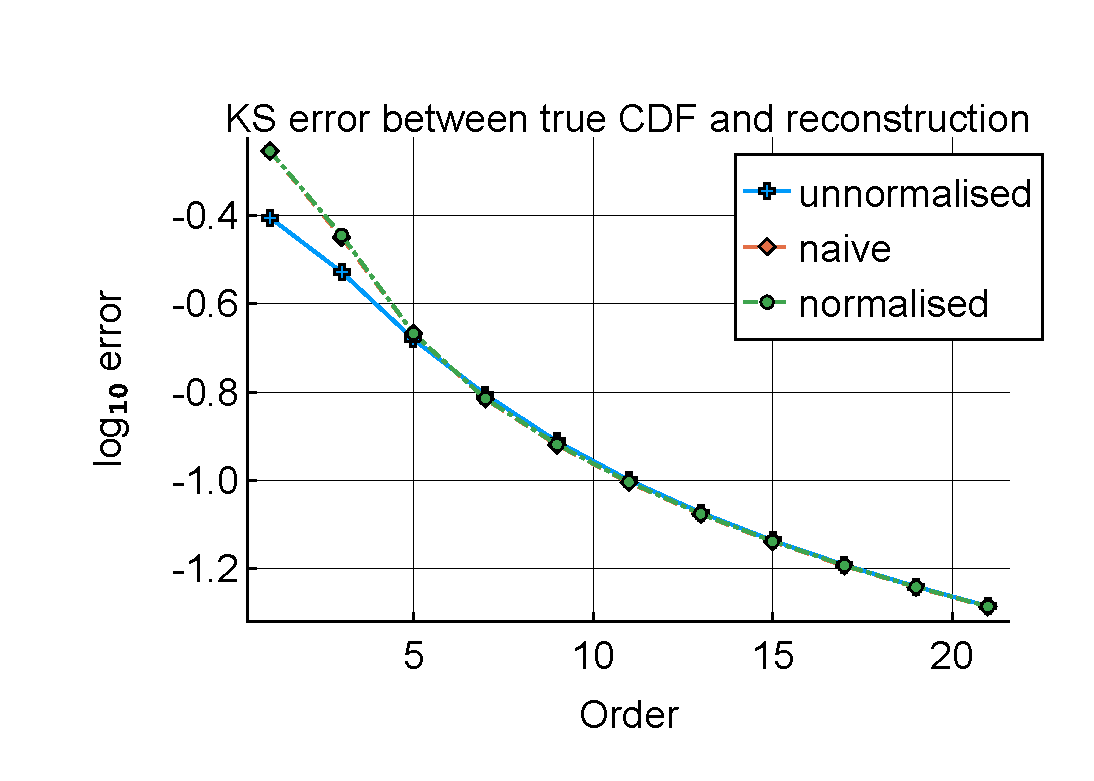
\includegraphics[width=0.5\textwidth,trim={1.25cm 0.8cm 0.25cm 1.25cm},clip]{chapter5/figs/qbdrap_closing_vec/fun2/ks_error_formatted.pdf}%
	\includegraphics[width=0.5\textwidth,trim={1.25cm 0.8cm 0.25cm 1.25cm},clip]{chapter5/figs/qbdrap_closing_vec/fun2/l2_pdf_error_formatted.pdf}
	\caption{KS error between the true CDF, \(2x1(x<0.5)+1(x\geq 0.5)\), and the approximations (left) and \(L^2\) error between the true PDF, \(2\times 1(x<0.5)\), and the approximations (right) for the three closing vectors considered; unnormalised (blue solid line with crosses), naive normalised (orange dashed line with diamonds) and normalised (green dash-dotted line with circles). The naive normalised (orange) an normalised closing vectors are coincident.}
	\label{fig: fun 2 ks error qbdrap closing vecs}
\end{figure}

Now consider approximating the initial density \(f(x)=1\). Observing Figure~\ref{fig: fun 4 ks error qbdrap closing vecs} of the KS error, and \(L^2\) error between the true initial distribution and the reconstructions, we now see that the normalised reconstructions outperform the unnormalised reconstruction. This suggests that, in this case, the `folding' of closing operator about \(\Delta\) has greatly increased the ability of the reconstruction to approximate this initial distribution. 
\begin{figure}
	\centering
	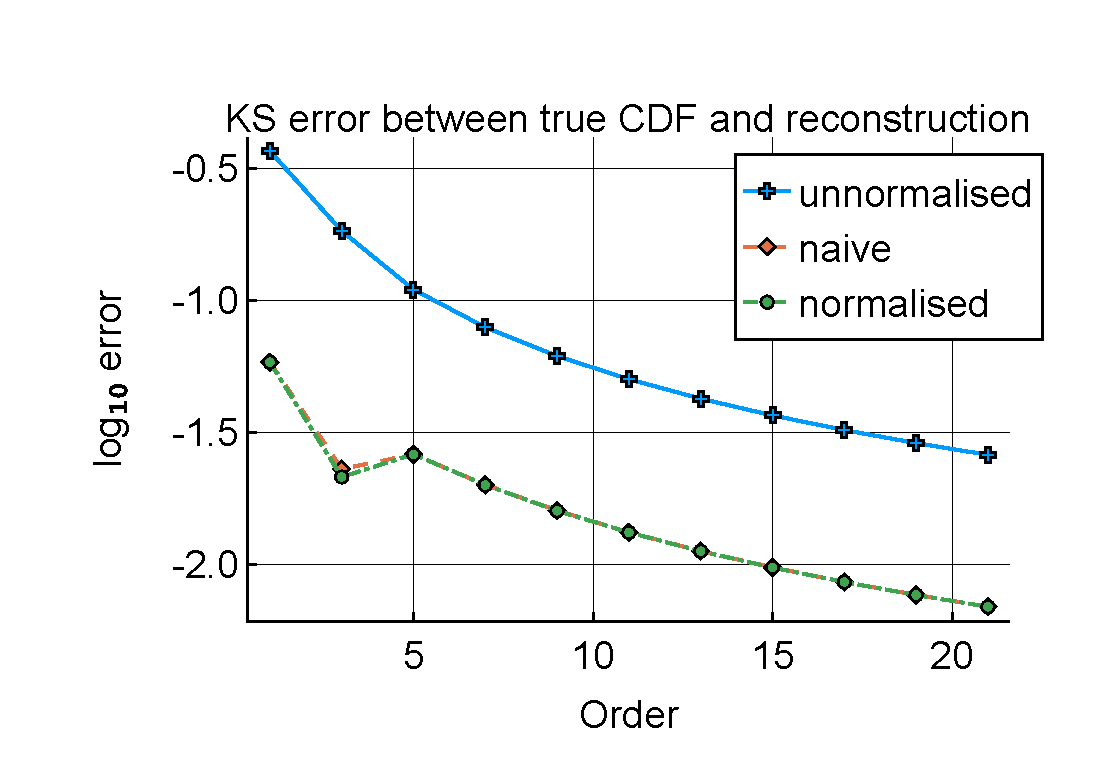
\includegraphics[width=0.5\textwidth,trim={1.25cm 0.8cm 0.25cm 1.25cm},clip]{chapter5/figs/qbdrap_closing_vec/fun4/ks_error_formatted.pdf}%
	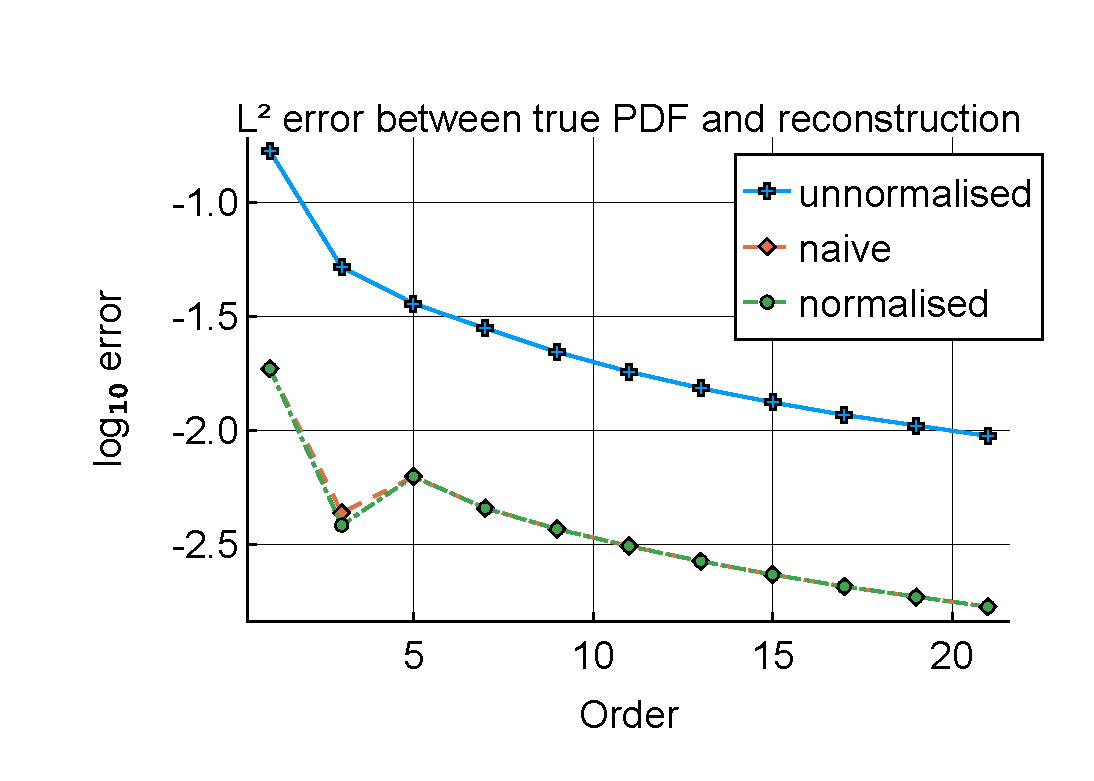
\includegraphics[width=0.5\textwidth,trim={1.25cm 0.8cm 0.25cm 1.25cm},clip]{chapter5/figs/qbdrap_closing_vec/fun4/l2_pdf_error_formatted.pdf}
	\caption{KS error between the true CDF, \(x\), and the approximation (left) and \(L^2\) error between the true PDF and the approximation (right) for the three closing vectors considered; unnormalised (blue solid line with crosses), naive normalised (orange dashed line with diamonds) and normalised (green dash-dotted line with circles). The naive normalised (orange) an normalised closing vectors are coincident.}
	\label{fig: fun 4 ks error qbdrap closing vecs}
\end{figure}

Some insight is gained by looking at Figure~\ref{fig: pdf reconstructed} where we plot the reconstructed PDFs for the unnormalised and normalised closing operators for order 1, 3, 5 and 7, as well as the true PDF. Observing Figure~\ref{fig: pdf reconstructed} notice that the unnormalised reconstruction fails to capture the density at the left of each of the plots and for all orders. This feature is due to a significant amount of mass being lost due to the truncation. In comparison the reconstruction with the normalised closing operator is much better in this region due to the `folding' around \(\Delta\) in the construction of the closing operator. In the reconstruction we also need to allocate the initial condition to a phase with positive rate, or negative rate, so that we can use the appropriate approximation and reconstruction method as discussed in Section~\ref{sec: closing}. Here we suppose that the phase is positive, so the `folding' around \(\Delta\) in the normalised closing operators appears appears at the left of the plots. In general, reconstructions via the unnormalised closing operator typically underestimate the value of the function in this region. 

Figure~\ref{fig: pdf reconstructed} also show that both closing operators do not approximate the initial condition well at the right-hand side of the interval. This is a common feature, and drawback, of the QBD-RAP method. Perhaps there is a different reconstruction method or yet another closing operator which could alleviate this issue. 
\begin{figure}
	\centering
	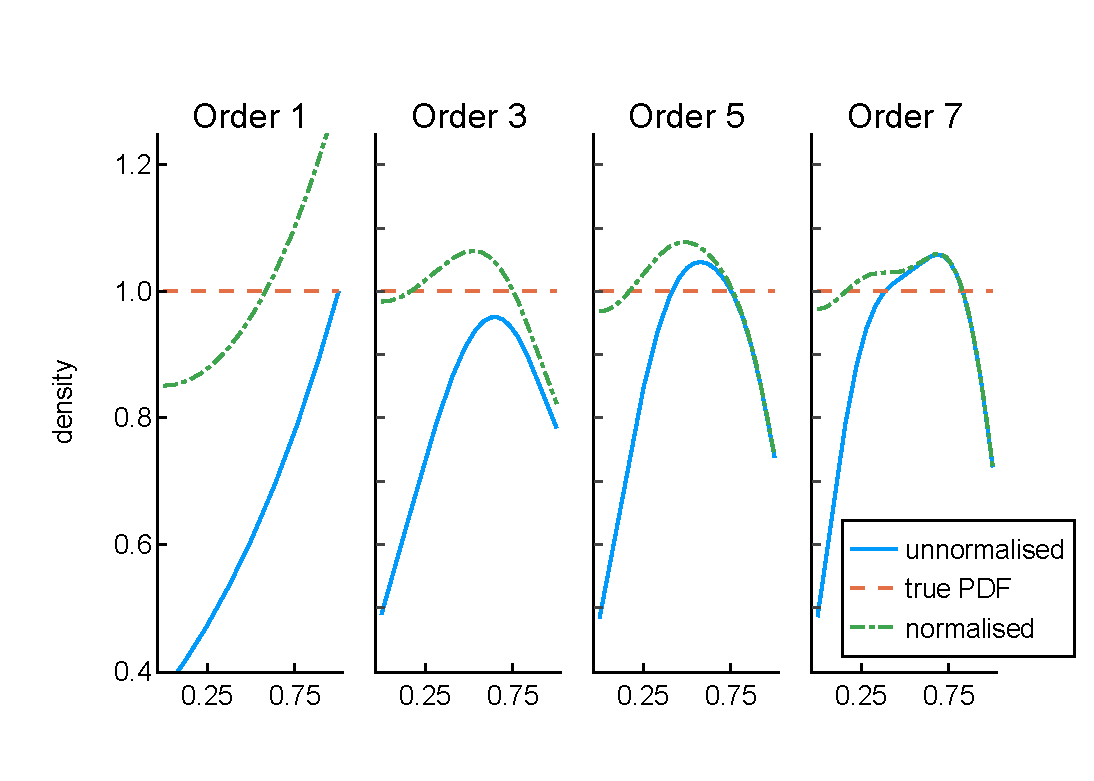
\includegraphics[width=\textwidth]{chapter5/figs/qbdrap_closing_vec/fun4/pdfs_formatted.pdf}
	\caption{Reconstructed PDFs using the unnormalised closing operator (blue solid line), normalised closing operator (green dash-dotted line), for various orders, and the true PDF which is \(f(x)=1\) (orange dashed line).}
	\label{fig: pdf reconstructed}
\end{figure} 

Next we consider approximating the initial distribution with density \(-6x^2+6x\). Observing the left-hand panel of Figure~\ref{fig: fun 6 ks error qbdrap closing vecs}, which plots the KS error against the order of the reconstruction for the three closing operators, we once again see that the reconstruction using the unnormalised closing operator performs the worst, while the performance of the two normalised reconstructions is indistinguishable. However, if we instead look at the right-hand panel of Figure~\ref{fig: fun 6 ks error qbdrap closing vecs}, which plots the \(L^2\) error between the reconstructed PDF and the true PDF, we see that with this metric, then unnormalised closing operator performs better than the two normalised ones for orders 5 and above. 
\begin{figure}
	\centering
	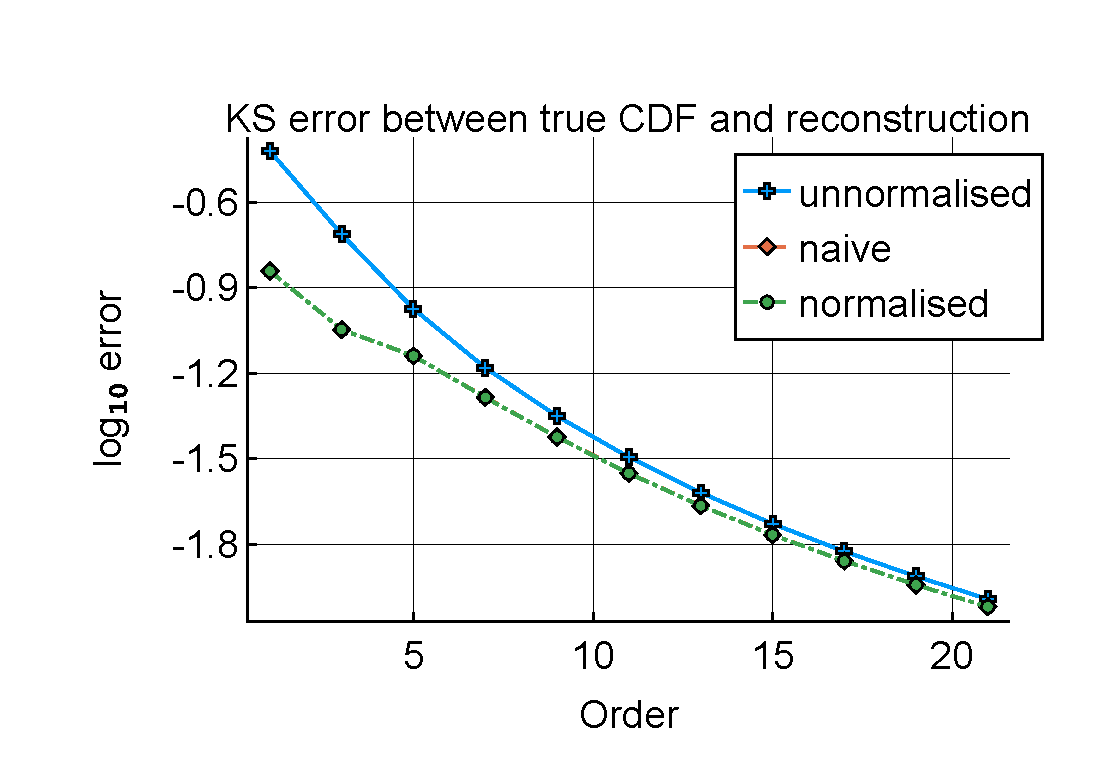
\includegraphics[width=0.5\textwidth,trim={1.25cm 0.8cm 0.25cm 1.25cm},clip]{chapter5/figs/qbdrap_closing_vec/fun6/ks_error_formatted.pdf}%
	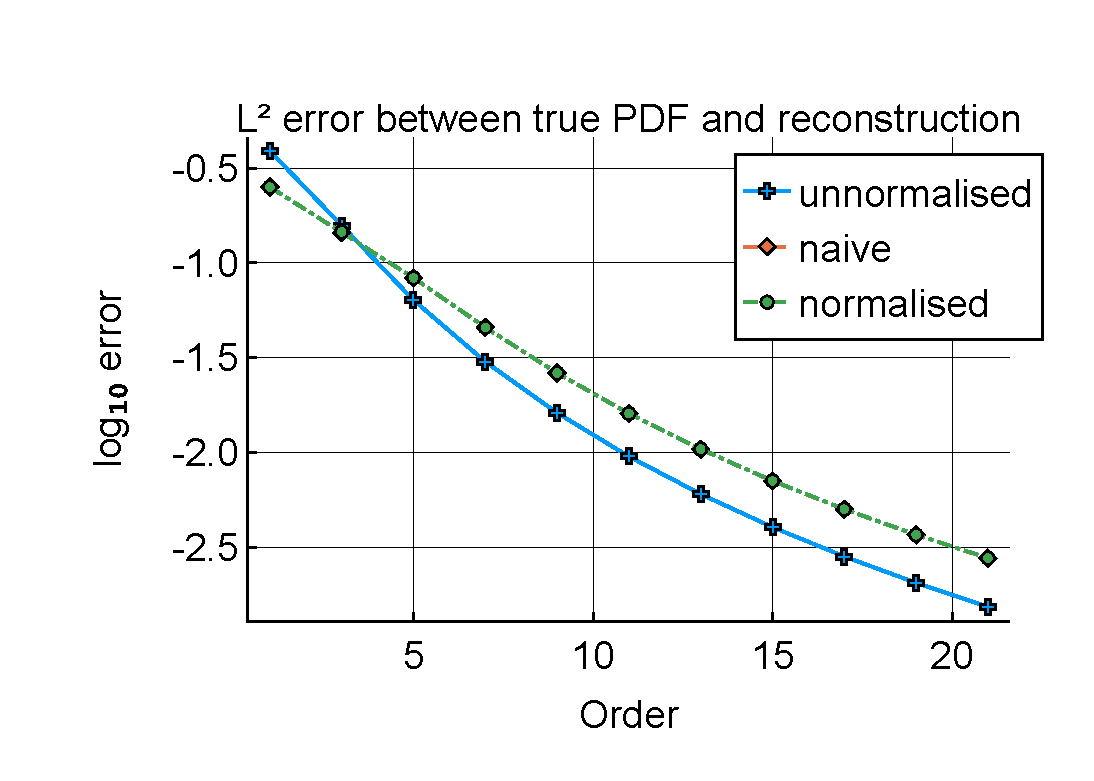
\includegraphics[width=0.5\textwidth,trim={1.25cm 0.8cm 0.25cm 1.25cm},clip]{chapter5/figs/qbdrap_closing_vec/fun6/l2_pdf_error_formatted.pdf}
	\caption{KS error between the true CDF, \(-2x^3+3x^2\), and the approximation (left) and \(L^2\) error between the true PDF \(-6x^2+6x\) and the approximation (right), for the three closing vectors considered; unnormalised (blue solid line with crosses), naive normalised (orange dashed line with diamonds) and normalised (green dash-dotted line with circles). The naive normalised (orange) an normalised closing vectors are coincident.}
	\label{fig: fun 6 ks error qbdrap closing vecs}
\end{figure}

The fact that the unnormalised closing operator outperforms the two normalised ones can be explain, once again, by the fact that, for the normalised operators we have `folded' the ME density function back on itself. In Figure~\ref{fig: pdf reconstructed quadratic} we plot the unnormalised and normalised reconstructions along with the true PDF, \(-6x^2+6x\). In Figure~\ref{fig: pdf reconstructed quadratic} we observe that, at the left of the plot, the normalised reconstructions over estimate the density function in this region, where as the unnormalised reconstruction looks to be doing better. Recall that the `folding' in the normalised closing operator manifest itself as extra mass at the left of these plots compared to the unnormalised reconstructions. 
\begin{figure}
	\centering
	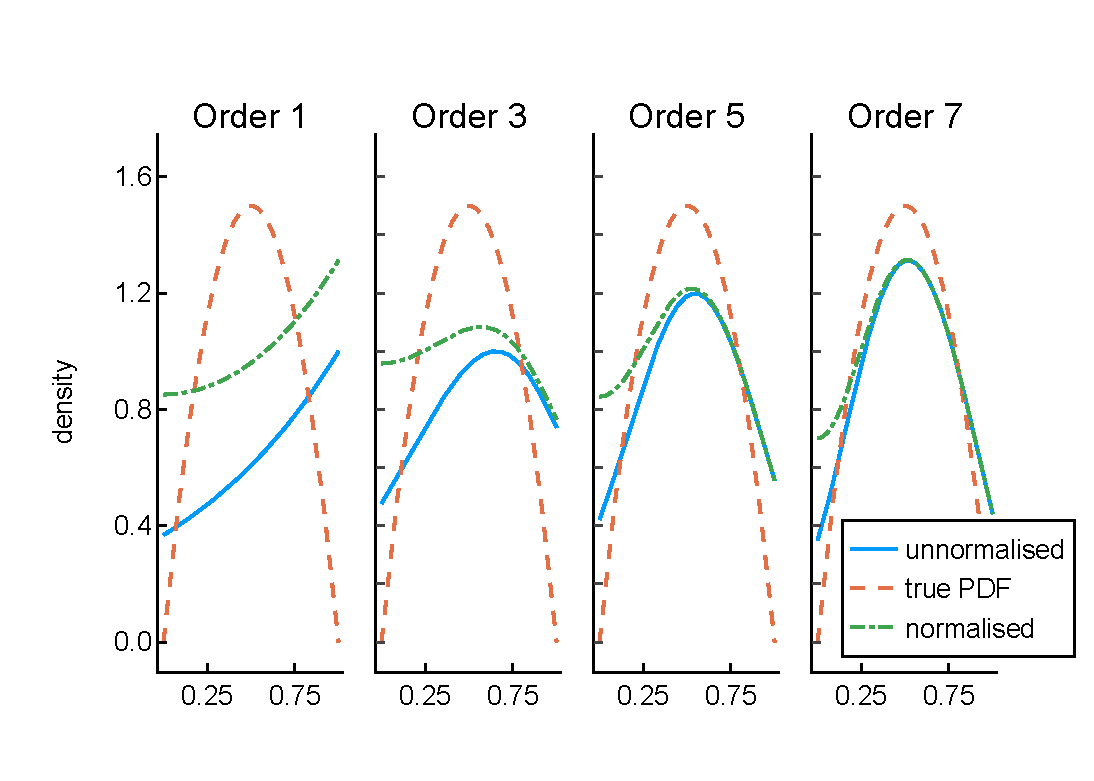
\includegraphics[width=\textwidth]{chapter5/figs/qbdrap_closing_vec/fun6/pdfs_formatted.pdf}
	\caption{Reconstructed PDFs using the unnormalised closing operator (blue solid line), normalised closing operator (green dash-dotted line), for various orders, and the true PDF which is \(f(x)=-6x^2+6x\) (orange dashed line).}
	\label{fig: pdf reconstructed quadratic}
\end{figure} 

Lastly, we consider approximating the initial distribution with PDF \(3e^{-3x}/(1-e^{-3})\). This density function is at a maximum at the left of the region. Considering what we have learnt so far about the unnormalised operator underestimating in this region, we expect that the unnormalised closing operator will perform relatively poorly in this case. Indeed, observing Figures~\ref{fig: fun 7 ks error qbdrap closing vecs} we see that the normalised reconstructions perform relatively well compared to the unnormalised reconstruction as measured by both error metrics (KS statistic and \(L^2\) norm on the PDF). If we observed plots of the PDFs (omitted), we would once again see that this is due to the loss of mass at the left-hand side of the region due to the truncation. 
\begin{figure}
	\centering
	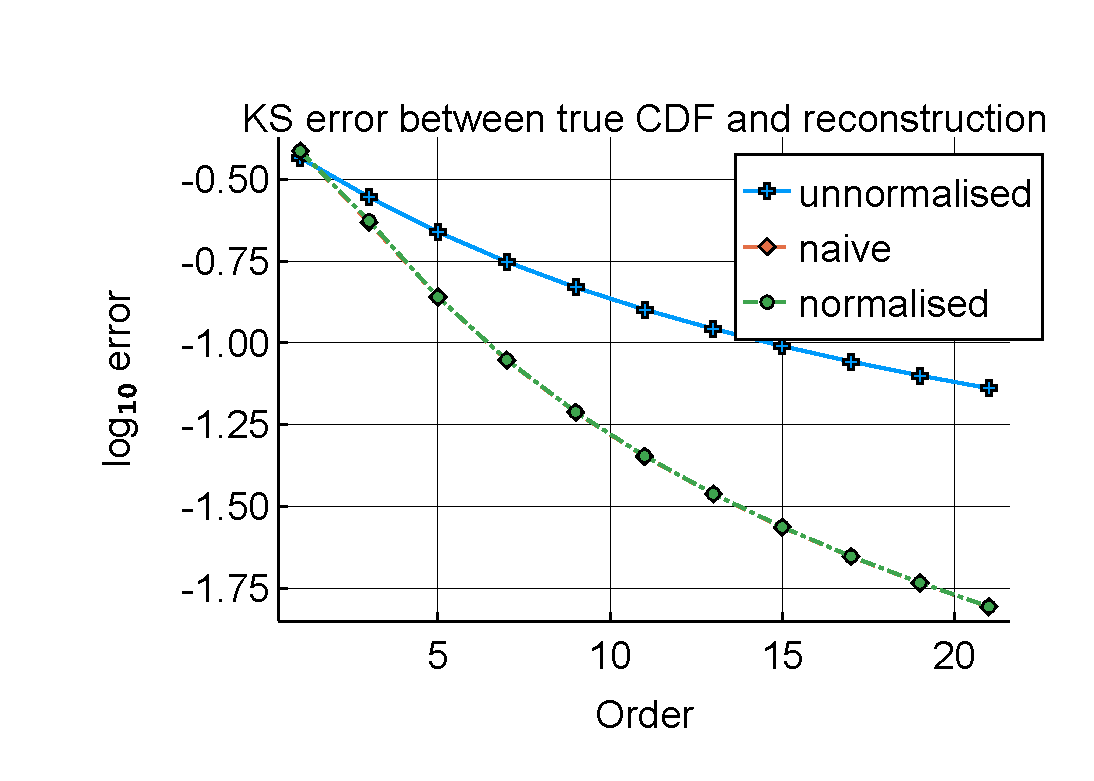
\includegraphics[width=0.5\textwidth,trim={1.25cm 0.8cm 0.25cm 1.25cm},clip]{chapter5/figs/qbdrap_closing_vec/fun7/ks_error_formatted.pdf}%
	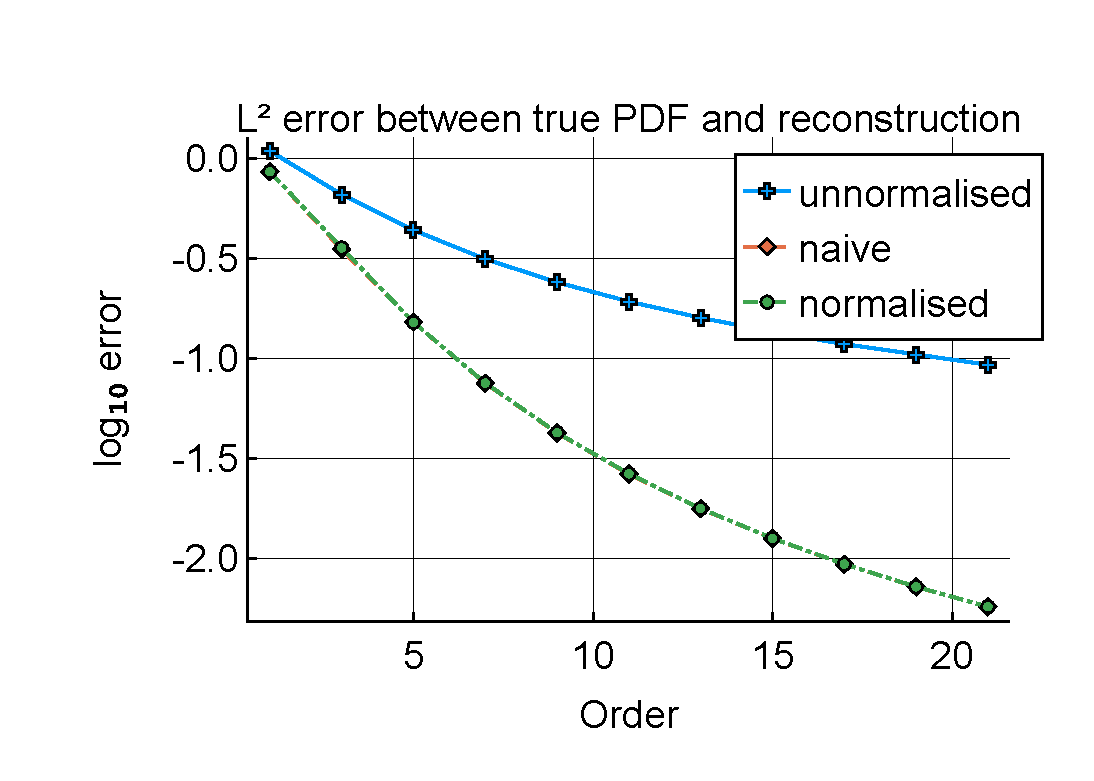
\includegraphics[width=0.5\textwidth,trim={1.25cm 0.8cm 0.25cm 1.25cm},clip]{chapter5/figs/qbdrap_closing_vec/fun7/l2_pdf_error_formatted.pdf}
	\caption{KS error between the true CDF, \((1-e^{-3x})/(1-e^{-3})\), and the approximation (left) and \(L^2\) error between the true PDF and the approximation for the three closing vectors considered; unnormalised (blue solid line with crosses), naive normalised (orange dashed line with diamonds) and normalised (green dash-dotted line with circles). The naive normalised (orange) an normalised closing vectors are coincident.}
	\label{fig: fun 7 ks error qbdrap closing vecs}
\end{figure}

Given the evidence above we choose to use the normalised closing operator to reconstruct solutions. Further, unlike the naive normalised operator, the normalised operator is theoretically justified in that we proved the closing operator leads to a convergent scheme and is linear. 

\subsection{Comparison of methods}
Here we compare the ability of the QBD-RAP, uniformisation, and DG methods to reconstruct initial conditions. 

First we consider the initial condition with CDF \(1(x\geq 0.5)\), that is, a point mass at 0.5. This distribution does not have a PDF so we can compare the CDFs only. In Figure~\ref{fig: fun 1 comp} we plot the KS metric (left) and \(L^1\) metric (right) between the true CDF and the reconstructed approximations. Observing the KS metric, it appears that none of the methods converge and the KS error sits around 0.5. This reflects the fact that convergence in distribution implies point-wise convergence of the CDFs except at points of discontinuity. None of the methods appear to converge at this point. Observing the \(L^1\) error between the true CDF and reconstructed approximation (which is the area between the two CDFs) we now see that the methods appear to show the convergent behaviour we expect. Here, the uniformisation method appears to perform the best, while the QBD-RAP method performs the worst. The rate of convergence of the QBD-RAP method appears to be similar to the rate of convergence of the DG scheme. 

Perhaps it is no surprise that the uniformisation method performs best. In the uniformisation method as we increase the order, we partition the cell \([0,1]\) into smaller sub-cells, and use constant functions on each sub-cell to approximate the function. As such, the uniformisation method can produce a piecewise continuous, linear approximation to the CDF. In contrast, both the DG and QBD-RAP methods result in a smooth approximation to the CDF. 
\begin{figure}
	\centering
	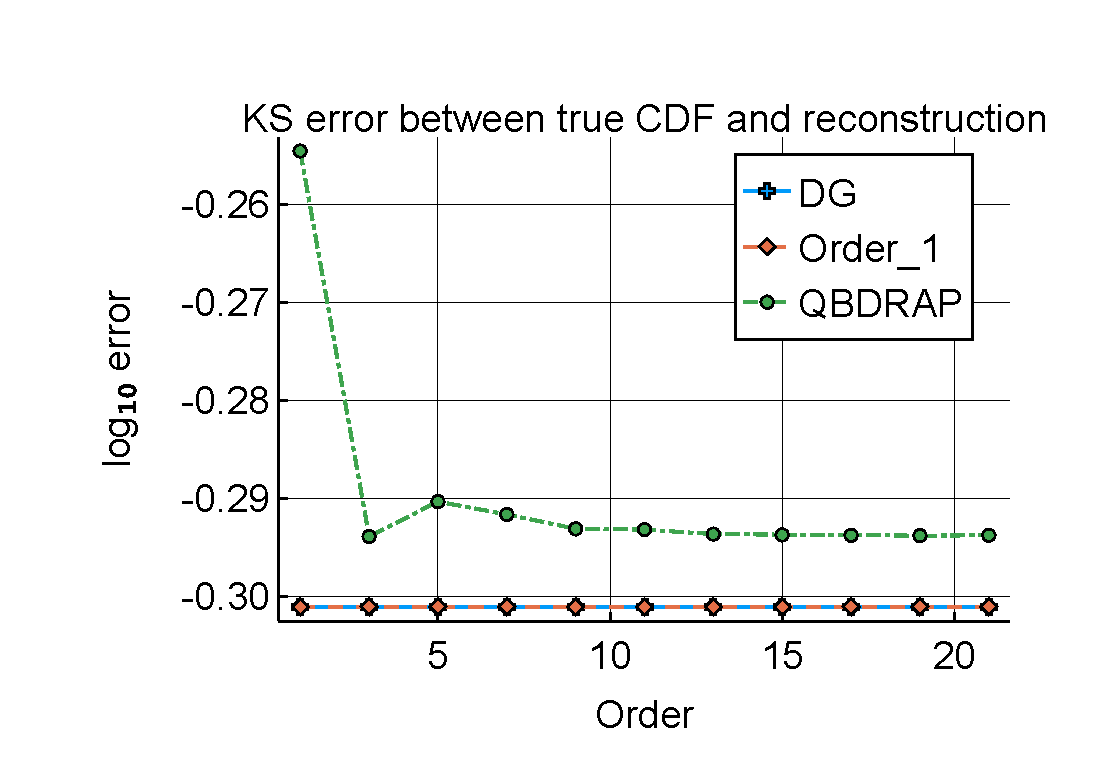
\includegraphics[width=0.5\textwidth,trim={1.25cm 0.8cm 0.25cm 1.25cm},clip]{chapter5/figs/comp/fun1/meshs_ks_error_formatted.pdf}%
	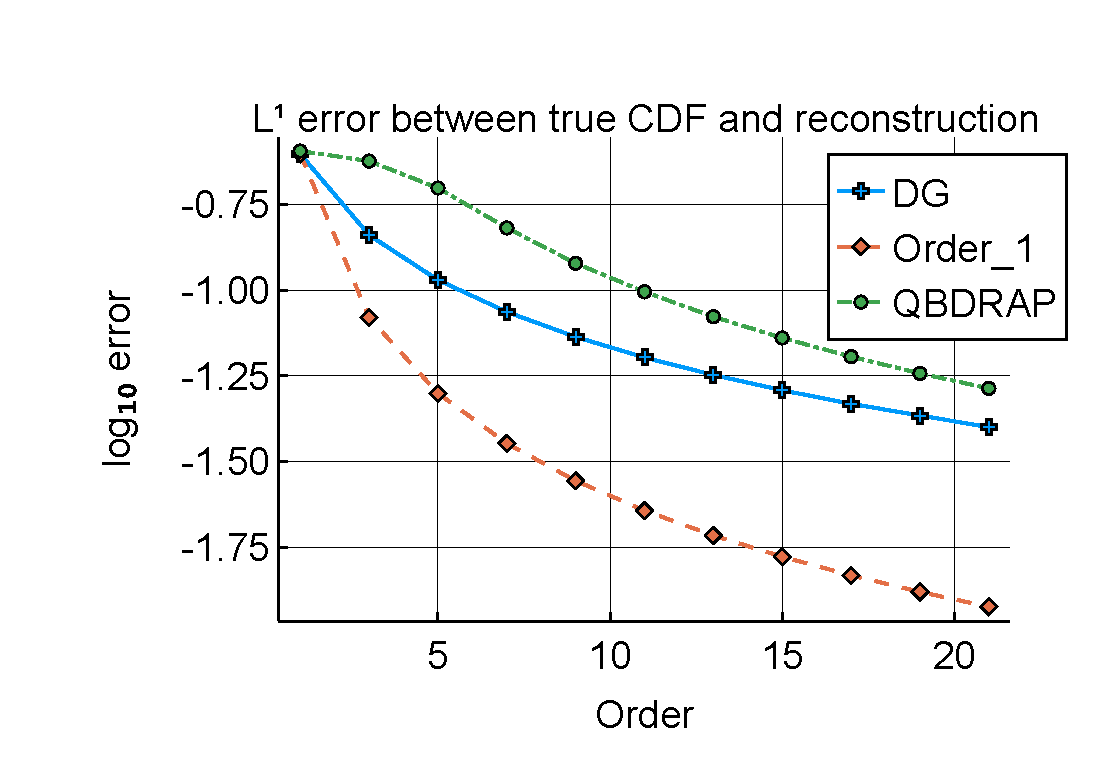
\includegraphics[width=0.5\textwidth,trim={1.25cm 0.8cm 0.25cm 1.25cm},clip]{chapter5/figs/comp/fun1/meshs_l1_cdf_error_formatted.pdf}
	\caption{KS error between the true CDF, \(1(x\geq 0.5)\), and the approximations (left) and \(L^1\) error between the true CDF and the approximations for the DG method (blue solid line with crosses), uniformisation method (orange dashed line with diamonds) and QBD-RAP method (green dash-dotted line with circles).}
	\label{fig: fun 1 comp} 
\end{figure}

In Figure~\ref{fig: pdf comp fun 1} we plot the approximated CDFs for the DG, uniformisation and QBD-RAP methods alongside the true CDF. The DG method displays undesirable features for an approximation to a CDF -- it is not monotonically increasing, at some points it is negative and at some points it is above 1. On the other hand, although the QBD-RAP method converges slowest, it displays good properties in that it results in a monotonically increasing CDF, starting at 0 and ending at 1. 
\begin{figure}
	\centering
	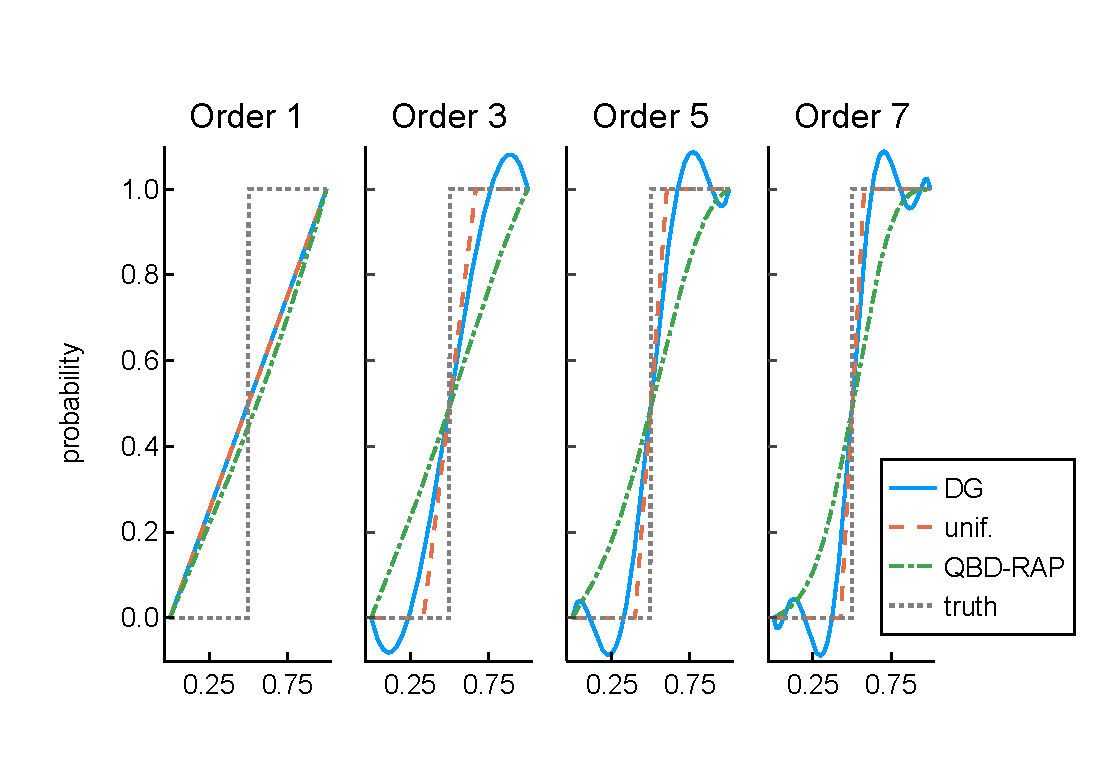
\includegraphics[width=\textwidth]{chapter5/figs/comp/fun1/cdfs_formatted.pdf}
	\caption{Reconstructed CDFs using the DG (blue solid line), uniformisation (orange dashed line) and QBD-RAP (green dot-dashed line) methods. The true distribution function is \(1(x\geq 0.5)\) (grey dotted line).}
	\label{fig: pdf comp fun 1}
\end{figure} 

Now consider approximating the initial distribution with PDF \(1(x\leq 0.5)\). Figure~\ref{fig: fun 2 comp} plots the KS error (left) and \(L^2\) error between the true and approximate PDFs (right). Figure~\ref{fig: fun 2 comp} suggests that all methods converge at a similar rate for this problem. Once again, the QBD-RAP method performs worst, the uniformisation method second, and the DG method the best. However, once again the DG method exhibits undesirable properties -- the approximation to the CDF is, at some points above 1, is not monotonic, though these violations are not as severe in this case as they were for the case above. 
\begin{figure}
	\centering
	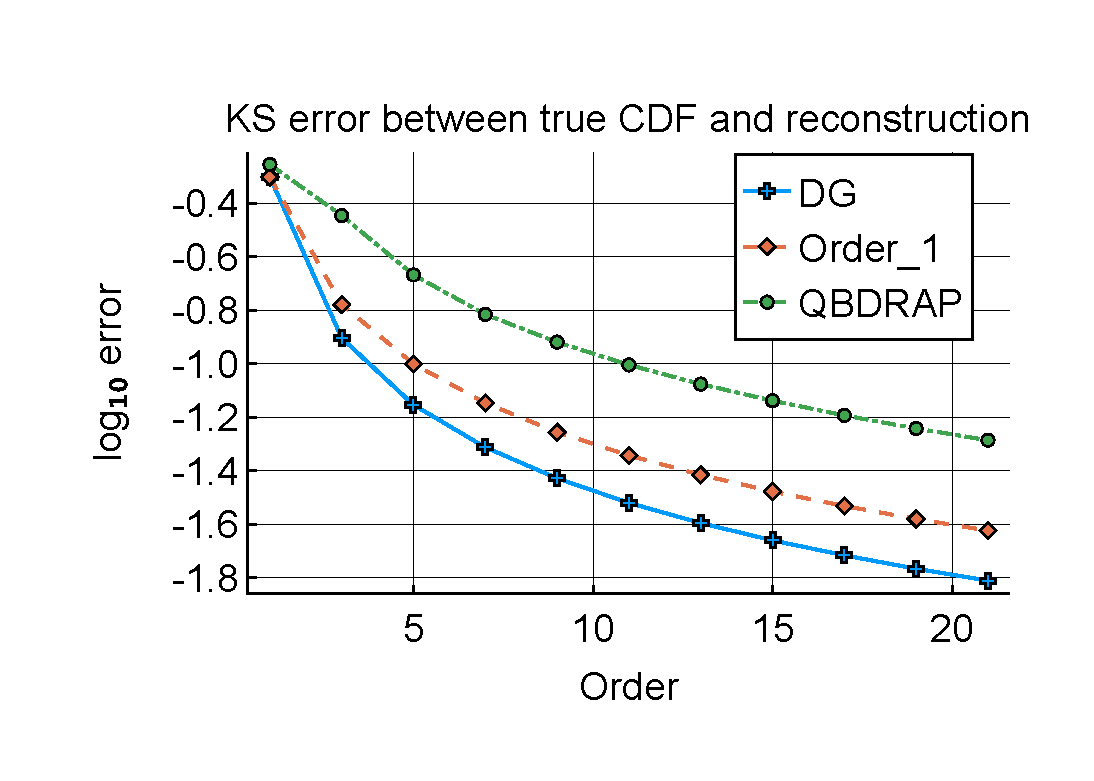
\includegraphics[width=0.5\textwidth,trim={1.25cm 0.8cm 0.25cm 1.25cm},clip]{chapter5/figs/comp/fun2/meshs_ks_error_formatted.pdf}%
	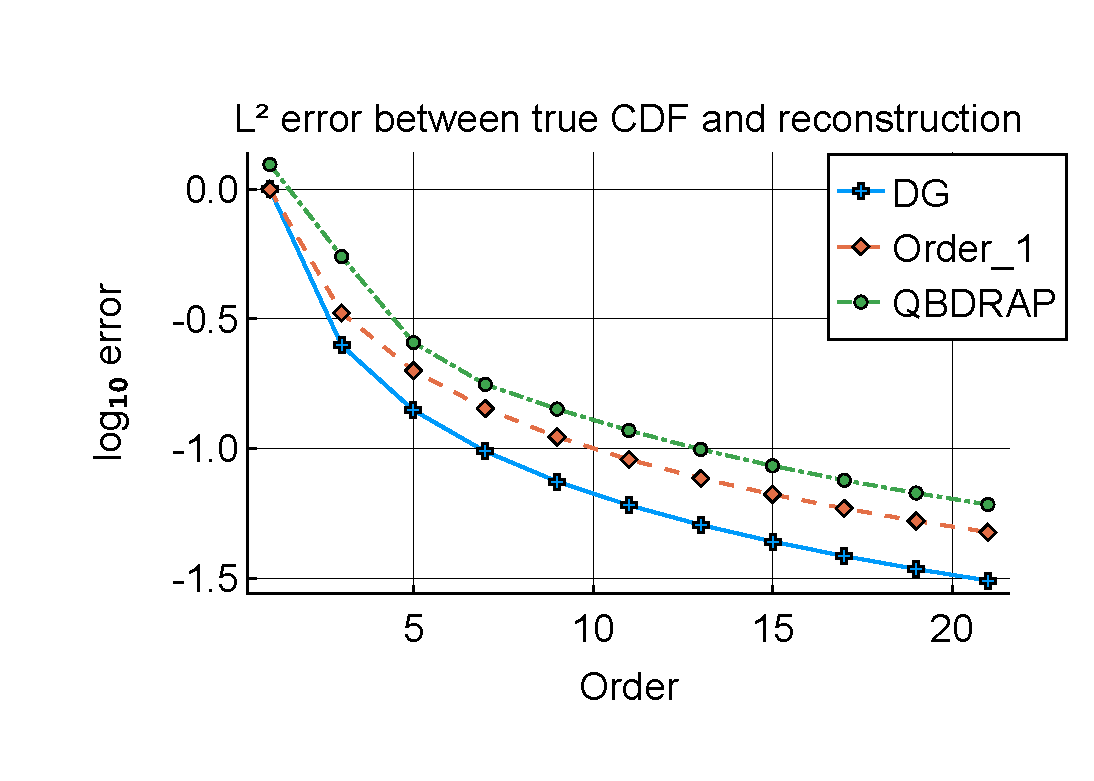
\includegraphics[width=0.5\textwidth,trim={1.25cm 0.8cm 0.25cm 1.25cm},clip]{chapter5/figs/comp/fun2/meshs_l2_pdf_error_formatted.pdf}
	\caption{KS error between the true CDF and the approximations (left) and \(L^2\) error between the true PDF, \(1(x\geq 0.5)\), and the approximations for the DG method (blue solid line with crosses), uniformisation method (orange dashed line with diamonds) and QBD-RAP method (green dash-dotted line with circles).}
	\label{fig: fun 2 comp} 
\end{figure}

So far we have considered two problems which exhibit discontinuities. At the other extreme we now consider an initial distribution with density \(-6z^2+6x\). In Figure~\ref{fig: fun 6 comp} we plot the KS error and the \(L^2\) error between the true and approximated PDF. Since the DG method projects the initial condition onto a polynomial basis, then, for an order 3 approximation and above, the DG method can theoretically approximate the initial condition exactly. This is reflected in Figure~\ref{fig: fun 6 comp}, where the blue curve drops sharply from 1-3, then plateaus. Due to numerical integration errors, for example in the evaluation of the integral in the \(L^2\) norm, and due to machine arithmetic, the errors for the DG scheme are not 0. Regarding the other two methods, they too appear to be convergent at approximately the same rate, with the uniformisation method perform better for the KS error, but very similarly in terms of the \(L^2\) error. 
\begin{figure}
	\centering
	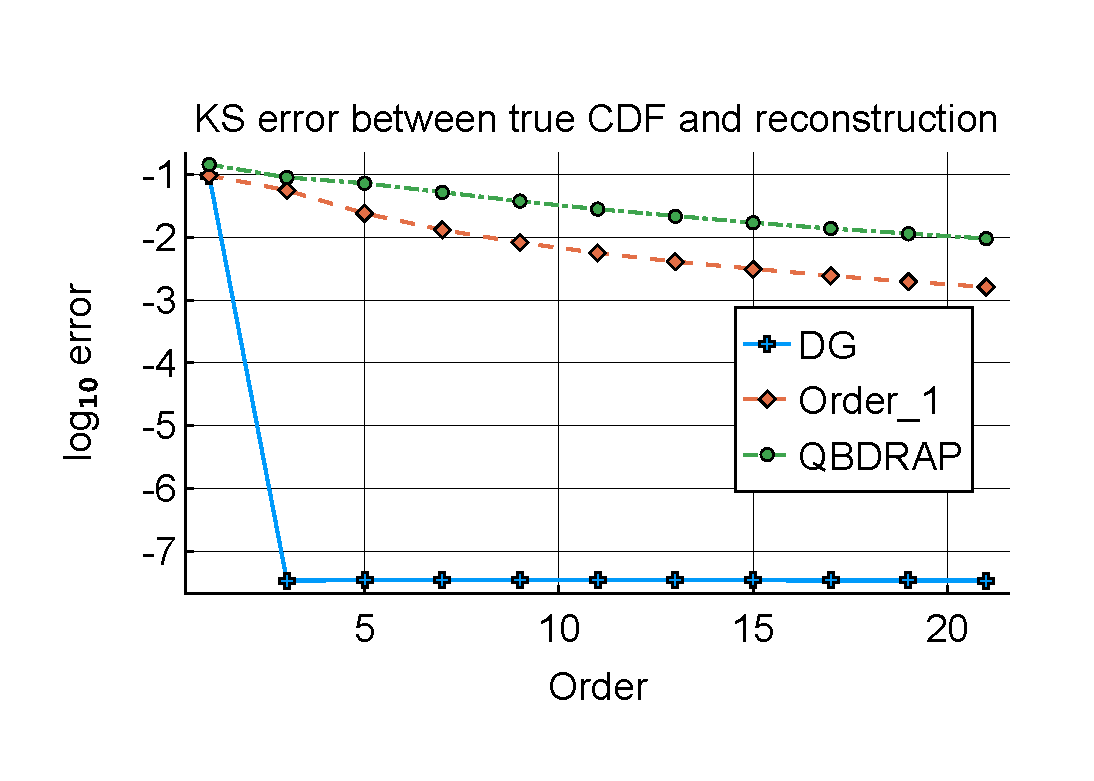
\includegraphics[width=0.5\textwidth,trim={1.25cm 0.8cm 0.25cm 1.25cm},clip]{chapter5/figs/comp/fun6/meshs_ks_error_formatted.pdf}%
	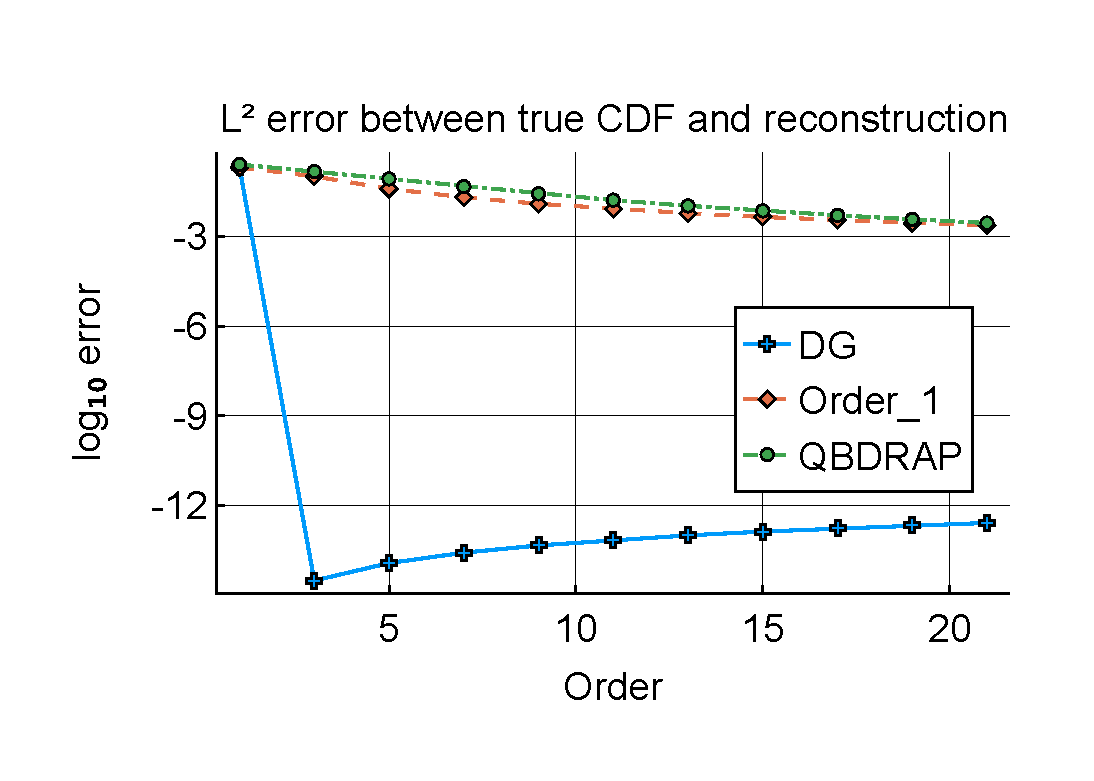
\includegraphics[width=0.5\textwidth,trim={1.25cm 0.8cm 0.25cm 1.25cm},clip]{chapter5/figs/comp/fun6/meshs_l2_pdf_error_formatted.pdf}
	\caption{KS error between the true CDF and the approximations (left) and \(L^2\) error between the true PDF, \(-6z^2+6x\), and the approximations for the DG method (blue solid line with crosses), uniformisation method (orange dashed line with diamonds) and QBD-RAP method (green dash-dotted line with circles).}
	\label{fig: fun 6 comp} 
\end{figure}

Consider now the initial distribution with PDF \(cos(4\pi(x+0.5))+1\). Figure~\ref{fig: fun 9 comp} shows the errors. Both the KS error (left) and \(L^2\) norm between the true and approximated PDFs tell a similar story. For sufficiently high order, the DG method approximates the inital condition very well. The uniformisation method performs second best, while the QBD-RAP method is slowest to converge. 
\begin{figure}
	\centering
	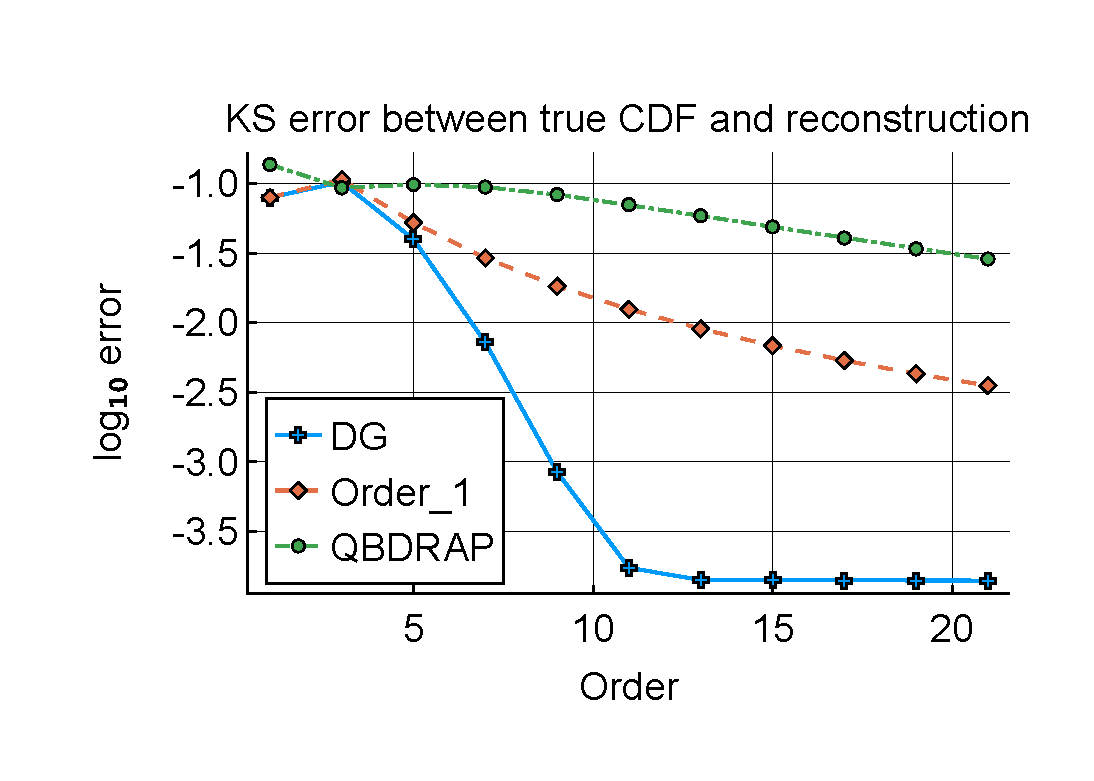
\includegraphics[width=0.5\textwidth,trim={1.25cm 0.8cm 0.25cm 1.25cm},clip]{chapter5/figs/comp/fun9/meshs_ks_error_formatted.pdf}%
	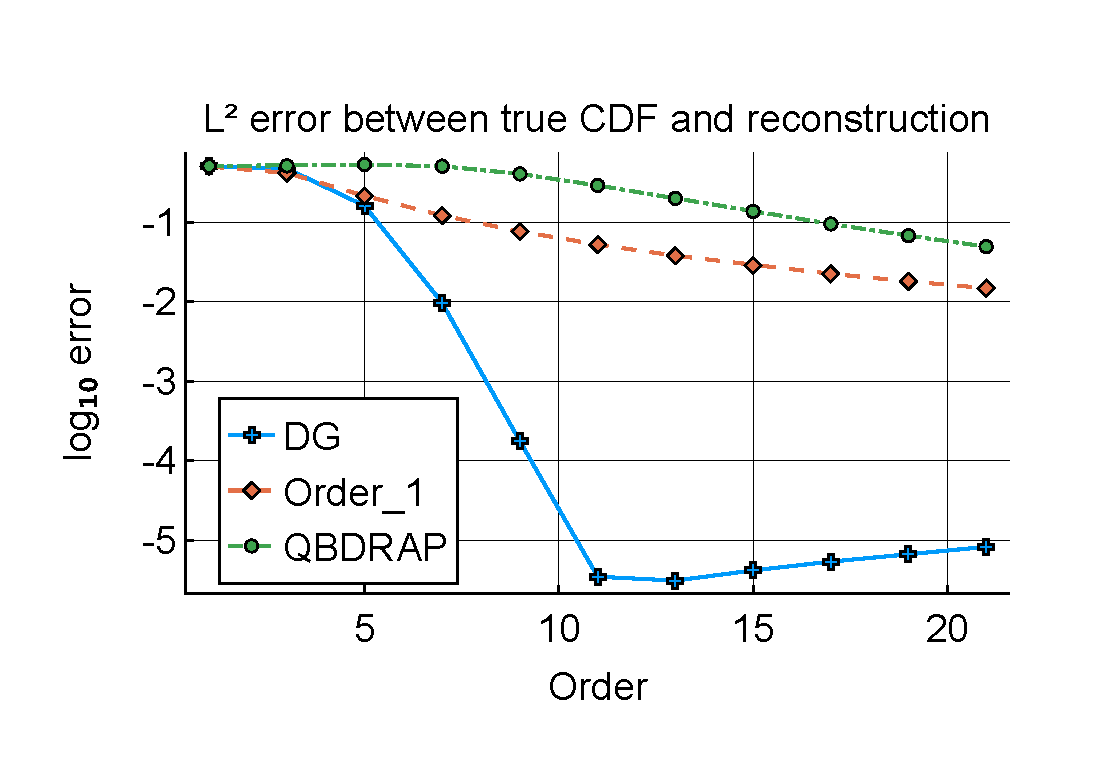
\includegraphics[width=0.5\textwidth,trim={1.25cm 0.8cm 0.25cm 1.25cm},clip]{chapter5/figs/comp/fun9/meshs_l2_pdf_error_formatted.pdf}
	\caption{KS error between the true CDF and the approximations (left) and \(L^2\) error between the true PDF, \(cos(4\pi(x+0.5))+1\), and the approximations for the DG method (blue solid line with crosses), uniformisation method (orange dashed line with diamonds) and QBD-RAP method (green dash-dotted line with circles).}
	\label{fig: fun 9 comp} 
\end{figure}
 
\FloatBarrier

\section{Travelling wave}
Here we investigate the performance the different schemes for approximating transient distributions of one-dimensional travelling wave problems with varying initial conditions. Consider a (trivial) fluid queue with one phase, generator \(\bs T=[0]\) and rate \(c=1\). The PDE (if/when it exists) which describes this system is 
\[\cfrac{\partial}{\partial t} f(x,t) = -\cfrac{\partial}{\partial x} f(x,t),\]
where \(f(x,t)\) is the density at time \(t\). Given an initial condition, \(f(x,0)\), solutions to this problem are given by 
\[f(x,t) = f(x-t,0)\]
so the solution at time \(t\) is just a shift in the initial condition \(t\) units to the right. We suppose that the fluid queue is bounded, with a lower boundary \(x=0\) and upper boundary \(x=10\). 

We use the QBD-RAP, uniformisation and DG schemes to discretise the solution in space. We discretise the interval \([0,10]\) into \(10\) cell, each of width 1. We use \(10,001\) points to approximate the integrals which appear in the construction of the initial conditions, to approximate the integrals appearing in the error metrics, and also as a set of discrete points on which evaluate the CDFs to approximate the KS metric. We use the SSPRK4 method to integrate over time using a step size of \(0.005\), and we evolve the system until time \(t=4\). For the DG method we also implement the Generalise MUSCL (REF, appendix?) slope limiter to stabilise the integration. 

First consider the initial condition with PDF \(1(x<1)\) so the level of the fluid queue is uniformly distributed over the first cell. For the DG and uniformisation methods, the initial condition can be represented exactly, whereas, for the QBD-RAP method, it cannot. Thus, in this case, there is no discretisation error in constructing the initial condition for the DG and uniformisation methods. 




































%!TEX root = ../thesis.tex
\chapter{Numerical investigations\label{sec: numerics}}
We have now established multiple methods for approximating fluid queues which suitable for approximating the performance measures for fluid-fluid queues derived in \cite{bo2014}. In this chapter we numerically investigate various aspects of the approximation schemes. Throughout, we compare the QBD-RAP scheme (from Chapters~\ref{sec: conv} and \ref{sec: construction and modelling}), the discontinuous Galerkin method (without limiters or filtering of the solution) (as decribed in Chapter~\ref{ch:galerkin}), and the spatially-coherent uniformisation as described in \cite{bo2013} (which we will refer to a just the \emph{uniformisation scheme}). Recall that the uniformisation scheme is equivalent to a discontinuous Galerkin scheme with a constant basis function in each cell, which is also equivalent to the finite-volume method with an upwind flux. Like the QBD-RAP scheme, due to its stochastic interpretation, the uniformisation scheme is positivity preserving. 


Where appropriate, we also compare the above methods with the discontinuous Galerkin method with a slope-limiter implemented, which avoids oscillations and negative solutions. However, recall that, in the context of approximating operators of fluid-fluid queues with these schemes, slope-limiting is not possible, and even when slope limiting is possible, the resultant approximation is at best linear around discontinuities. 

The main focus of our numerical experiments is on the convergence properties as the number of basis functions is increased. For discontinuous Galerkin method, this means increasing the number of basis functions used to approximate the solution within each cell. For the QBD-RAP scheme, this means increasing the order of the CME distribution used to construct the scheme. For the uniformisation scheme, this means dividing each cell into smaller sub-cells over which we approximate the solution. As such, each approximation scheme leads to approximations which are matrices of the same size (although not necessarily the same number of non-zero components). For example, if we use 3 basis functions in the discontinuous Galerkin method, we approximate the solution by a quadratic on each cell; the comparable QBD-RAP scheme is to use a CME of order 3; and the comparable uniformisation scheme is to divide each cell into 3 sub-cells of width \(\Delta/3\). 

To keep the content of this chapter contained, we do not investigate the performance of the schemes as the cell sizes are decreased, other than for the uniformisation scheme. As such, for each numerical experiment, we keep the cell size fixed. As part of deriving a discontinuous Galerkin scheme, one needs to choose the \emph{numerical flux} which is used to approximate the transition of density from one cell to the next and link all the cells together. We investigate schemes with an upwind flux only.
We do not investigate the stability of the schemes with respect to the step-size of the time-integration or time-integration scheme (where required). Instead, we fix the time-integration step size for each numerical experiment at a suitably small value so as to obey a certain stability criterion (a CFL-like condition, REFs, appendix?). For schemes which require us to integrate over time we always implement the strong stability preserving Runge-Kutta method of order 4 with 5 stages (see appendix and REF). This scheme claims to introduce no more oscillations into the solution as we integrate over time (REFs). Where a slope limiter is implemented, we always implement the \emph{Generalised MUSCL} limiter (REF and Appendix). We do not investigate filtering for the DG scheme (REFs).

The performance of the discontinuous Galerkin method has been well-studied (REFs), and it is well-known that the discontinuous Galerkin method performs remarkably well on problems with smooth solutions (REF). Here, we mostly focus on investigating the numerical performance of the methods on problems with non-smooth solutions, the purpose of this is to emphasise the positivity-preserving properties of the QBD-RAP method. In the stochastic modelling community it is very common to have problems with discontinuous solutions, such as a non-smooth initial conditions (REFs). Even if a fluid-queue is initialised with a smooth initial density, the boundary dynamics may induce transient discontinuities into the problem. There is a very specific set of conditions on the initial density and point masses which must hold for the distribution of the fluid queue to remain smooth as it evolves over time (REFs).Limiting distributions of fluid queues are smooth, however. Further, it is possible that discontinuities are present in the performance measures of fluid-fluid queues. 

As we shall see, if the solution is smooth, then the Galerkin method is highly-effective and displays rapid convergence to the solution as the number polynomial basis functions is increased. However, when the solution is non-smooth oscillations and negative approximations may occur when using the discontinuous Galerkin method, leading to non-sensical solutions. In these cases, the QBD-RAP approximation performs relatively well compared to the other positivity preserving schemes investigated.

% THE STRUCTURE OF THE CHAPTER IS AS FOLLOWS. 

% 1. FUNCTION APPROX./RECONSTRUCTION

% 2. 1d wave eqn

% 3. STATIONARY DISTRIBUTIONS
	% i. SIMPLER
	% ii. MORE COMPLEX
	
% 4. TRANSIENT DISTRIBUTIONS 
	% i. SIMPLER
	% ii. MORE COMPLEX

% 5. HITTING TIMES 
	% i. SIMPLER
	% ii. MORE COMPLEX

% 6. FLUID-FLUID QUEUES

% 7. CONCLUDING REMARKS 

\section{Function approximation/reconstruction}
We start our investigation by looking at how well the methods perform at approximating an initial condition. For the discontinuous Galerkin method, this means projecting the solution on to the set of polynomial functions which define the scheme, then reconstructing the solution. For the spatially-coherent uniformisation scheme, this means looking at the sub-cell averages. For the QBD-RAP scheme, this means computing the initial vector for the approximation, then reconstructing the solutions as described in Section~\ref{sec: closing}. First we investigate three closing vectors we can use for the reconstruction for the QBD-RAP, from which we find that the closing operator in (\ref{eqn:5462}) performs reasonably compared to the others, and we are able to theoretically prove that it converges. Therefore we use this reconstruction method throughout the rest of the chapter.

For this section we consider approximating the initial condition over a single cell of width \(\Delta = 1\). To numerically evaluate integrals arising in the approximation step (inner products and cell averages) we use a simple trapezoidal rule with 10,001 function evaluations. Similarly, we use 10,001 function evaluations to approximate \(L^2\) norms, and also as a finite set of points over which to compute the KS statistics. 

First we briefly investigate the possible choices of closing operators as introduced in Section~\ref{sec: closing}. 

\subsection{QBD-RAP closing operators}
The three closing operators we investigate are the following. The unnormalised closing vector in Equation~(\ref{eqn: alal}). A normalised version of the closing operator in Equation~(\ref{eqn:546}), with the normalised version given by (\ref{eqn: nonlin}). We refer to the closing vector in (\ref{eqn: nonlin}) as the \emph{naive normalised} closing vector. Technically we have not yet proved that the \emph{naive normalised} closing vector leads to a convergent approximation scheme, though it clearly appears to converge. The third closing vector we investigate is that in Equation~(\ref{eqn:5462}). 

\begin{example}First consider approximating the initial condition with density function \(1(x<0.5)\). In the left-hand side of Figure~\ref{fig: fun 2 ks error qbdrap closing vecs} we plot the Kolmogorov-Smirnov error between the true CDF and the CDF constructed via the QBD-RAP approximation. Interestingly, in this case, the unnormalised error outperforms the other two reconstructions at low orders. It just so happens that, in this case, the error due to truncation of the unnormalised reconstruction destructively interferes with other errors in the reconstruction to cause the error to be lower at low orders for the unnormalised scheme. Figure~\ref{fig: fun 2 ks error qbdrap closing vecs} also shows that the naive normalised and normalised reconstructions perform very similarly -- this is the case throughout much of this subsection. The difference between the naive normalised and normalised reconstructions is how they treat mass in the tail of a matrix exponential distribution (from \(2\Delta\) onward). Intuitively, there should be very little mass in the tail of the distribution as we are using concentrated matrix exponential distributions in the reconstruction. 

If we instead look at the \(L^2\) error between the true PDF and the reconstructions in Figure~\ref{fig: fun 2 ks error qbdrap closing vecs}, then we see that the unnormalised reconstruction performs the poorest. Figure~\ref{fig: fun 2 ks error qbdrap closing vecs} also suggests naive normalised and normalised reconstruction are very similar. 
\begin{figure}
	\centering
	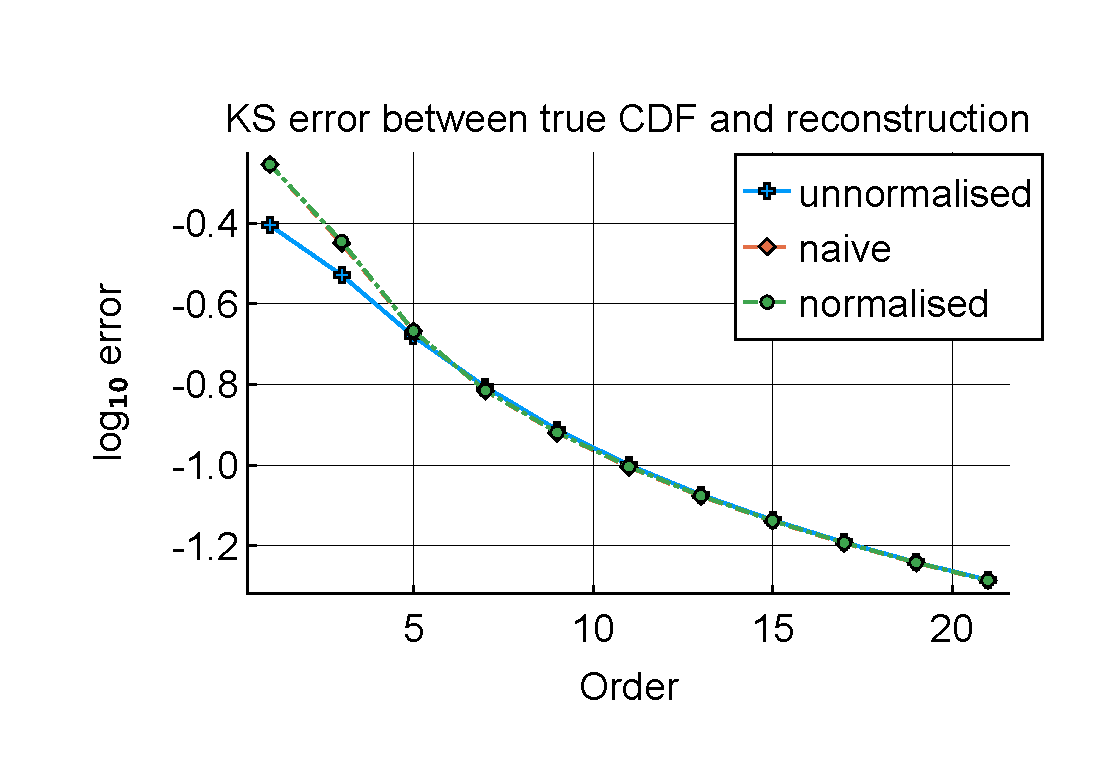
\includegraphics[width=0.5\textwidth,trim={1.25cm 0.8cm 0.25cm 1.25cm},clip]{chapter6/figs/qbdrap_closing_vec/fun2/ks_error_formatted.pdf}%
	\includegraphics[width=0.5\textwidth,trim={1.25cm 0.8cm 0.25cm 1.25cm},clip]{chapter6/figs/qbdrap_closing_vec/fun2/l2_pdf_error_formatted.pdf}
	\caption{KS error between the true CDF, \(2x1(x<0.5)+1(x\geq 0.5)\), and the approximations (left) and \(L^2\) error between the true PDF, \(2\times 1(x<0.5)\), and the approximations (right) for the three closing vectors considered; unnormalised (blue solid line with crosses), naive normalised (orange dashed line with diamonds) and normalised (green dash-dotted line with circles). The naive normalised (orange) an normalised closing vectors are coincident.}
	\label{fig: fun 2 ks error qbdrap closing vecs}
\end{figure}
\end{example}

\begin{example}Now consider approximating the initial density \(f(x)=1\). Observing Figure~\ref{fig: fun 4 ks error qbdrap closing vecs} of the KS error, and \(L^2\) error between the true initial distribution and the reconstructions, we now see that the normalised reconstructions outperform the unnormalised reconstruction. This suggests that, in this case, the `folding' of closing operator about \(\Delta\) has greatly increased the ability of the reconstruction to approximate this initial distribution. 
\begin{figure}
	\centering
	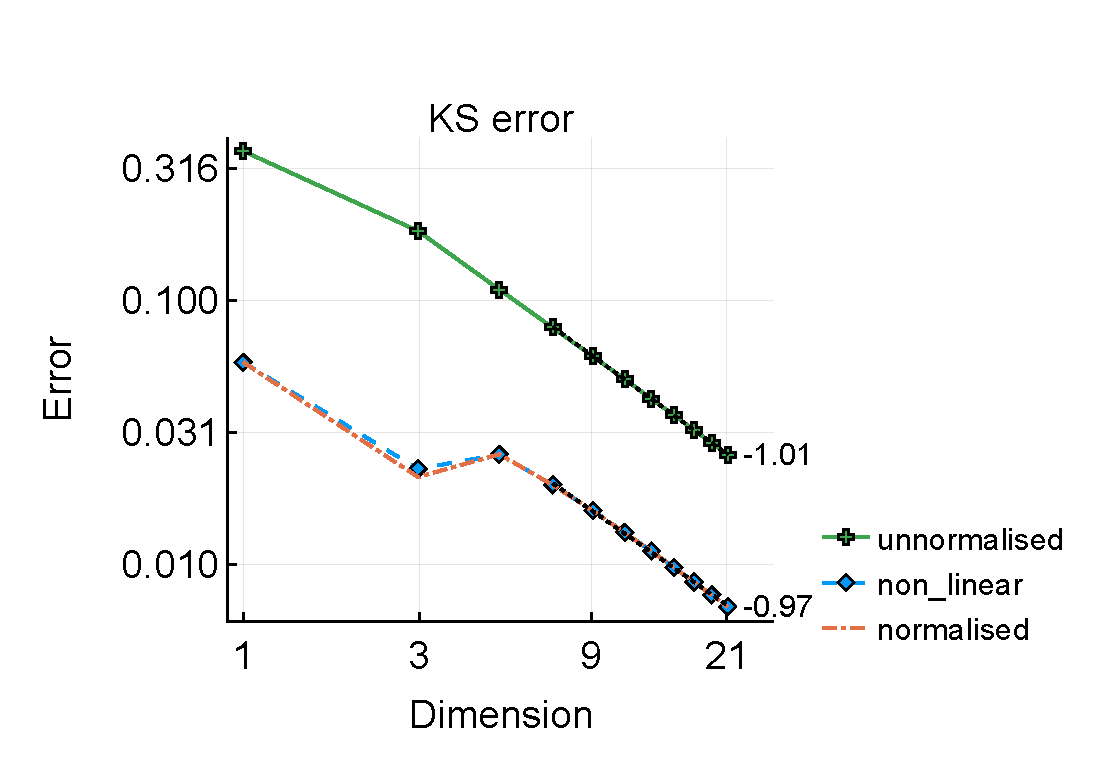
\includegraphics[width=0.5\textwidth,trim={1.25cm 0.8cm 0.25cm 1.25cm},clip]{chapter6/figs/qbdrap_closing_vec/fun4/ks_error_formatted.pdf}%
	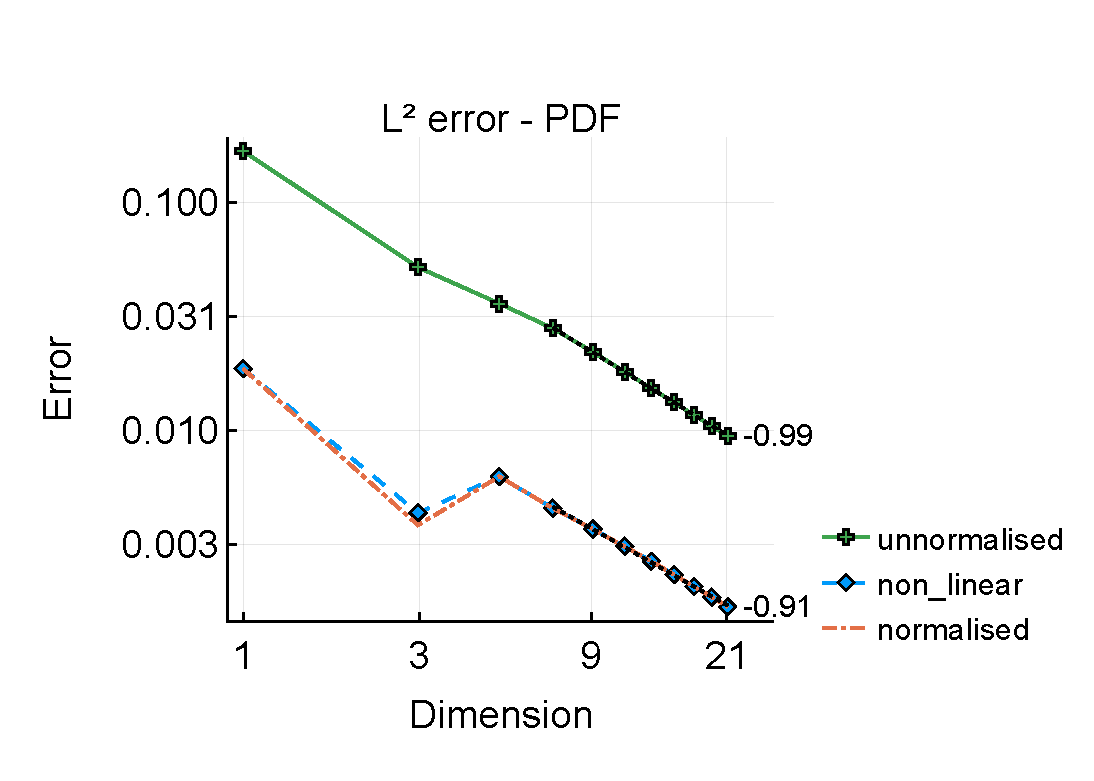
\includegraphics[width=0.5\textwidth,trim={1.25cm 0.8cm 0.25cm 1.25cm},clip]{chapter6/figs/qbdrap_closing_vec/fun4/l2_pdf_error_formatted.pdf}
	\caption{KS error between the true CDF, \(x\), and the approximation (left) and \(L^2\) error between the true PDF and the approximation (right) for the three closing vectors considered; unnormalised (blue solid line with crosses), naive normalised (orange dashed line with diamonds) and normalised (green dash-dotted line with circles). The naive normalised (orange) an normalised closing vectors are coincident.}
	\label{fig: fun 4 ks error qbdrap closing vecs}
\end{figure}

Some insight is gained by looking at Figure~\ref{fig: pdf reconstructed} where we plot the reconstructed PDFs for the unnormalised and normalised closing operators for order 1, 3, 5 and 7, as well as the true PDF. Observing Figure~\ref{fig: pdf reconstructed} notice that the unnormalised reconstruction fails to capture the density at the left of each of the plots and for all orders. This feature is due to a significant amount of mass being lost due to the truncation. In comparison the reconstruction with the normalised closing operator is much better in this region due to the `folding' around \(\Delta\) in the construction of the closing operator. In the reconstruction we also need to allocate the initial condition to a phase with positive rate, or negative rate, so that we can use the appropriate approximation and reconstruction method as discussed in Section~\ref{sec: closing}. Here we suppose that the phase is positive, so the `folding' around \(\Delta\) in the normalised closing operators appears appears at the left of the plots. In general, reconstructions via the unnormalised closing operator typically underestimate the value of the function in this region. 

Figure~\ref{fig: pdf reconstructed} also show that both closing operators do not approximate the initial condition well at the right-hand side of the interval. This is a common feature, and drawback, of the QBD-RAP method. Perhaps there is a different reconstruction method or yet another closing operator which could alleviate this issue. 
\begin{figure}
	\centering
	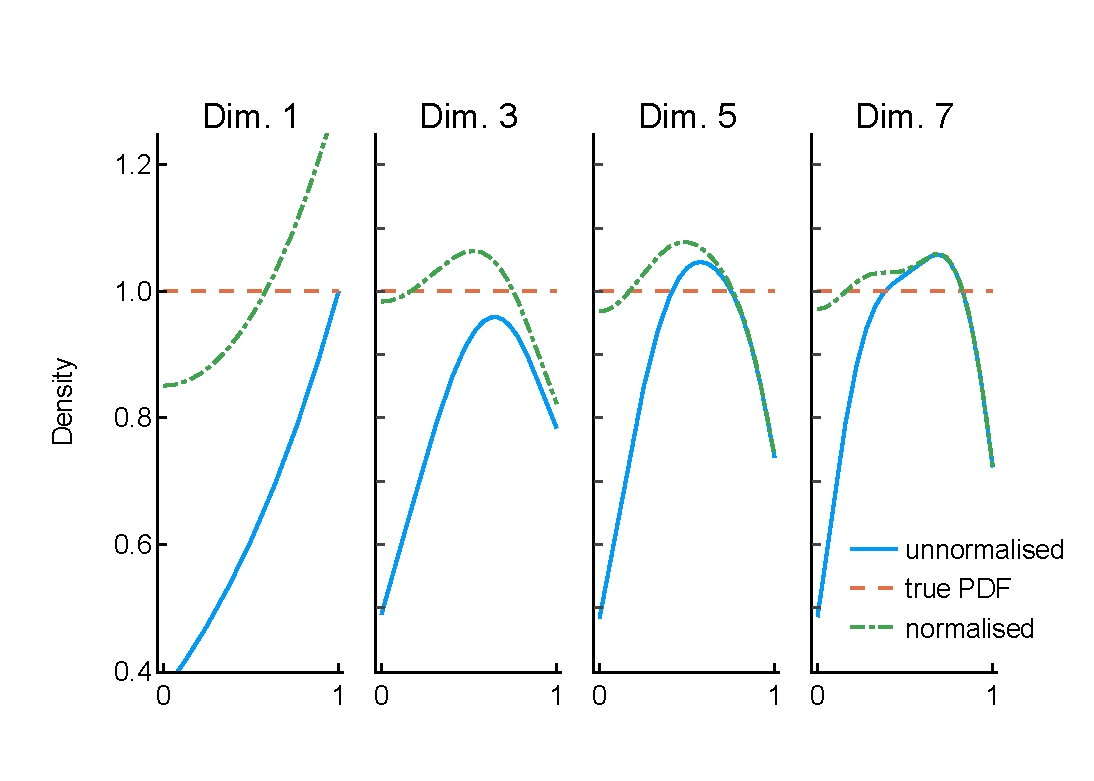
\includegraphics[width=\textwidth]{chapter6/figs/qbdrap_closing_vec/fun4/pdfs_formatted.pdf}
	\caption{Reconstructed PDFs using the unnormalised closing operator (blue solid line), normalised closing operator (green dash-dotted line), for various orders, and the true PDF which is \(f(x)=1\) (orange dashed line).}
	\label{fig: pdf reconstructed}
\end{figure} 
\end{example}

\begin{example}Next we consider approximating the initial distribution with density \(-6x^2+6x\). Observing the left-hand panel of Figure~\ref{fig: fun 6 ks error qbdrap closing vecs}, which plots the KS error against the order of the reconstruction for the three closing operators, we once again see that the reconstruction using the unnormalised closing operator performs the worst, while the performance of the two normalised reconstructions is indistinguishable. However, if we instead look at the right-hand panel of Figure~\ref{fig: fun 6 ks error qbdrap closing vecs}, which plots the \(L^2\) error between the reconstructed PDF and the true PDF, we see that with this metric, then unnormalised closing operator performs better than the two normalised ones for orders 5 and above. 
\begin{figure}
	\centering
	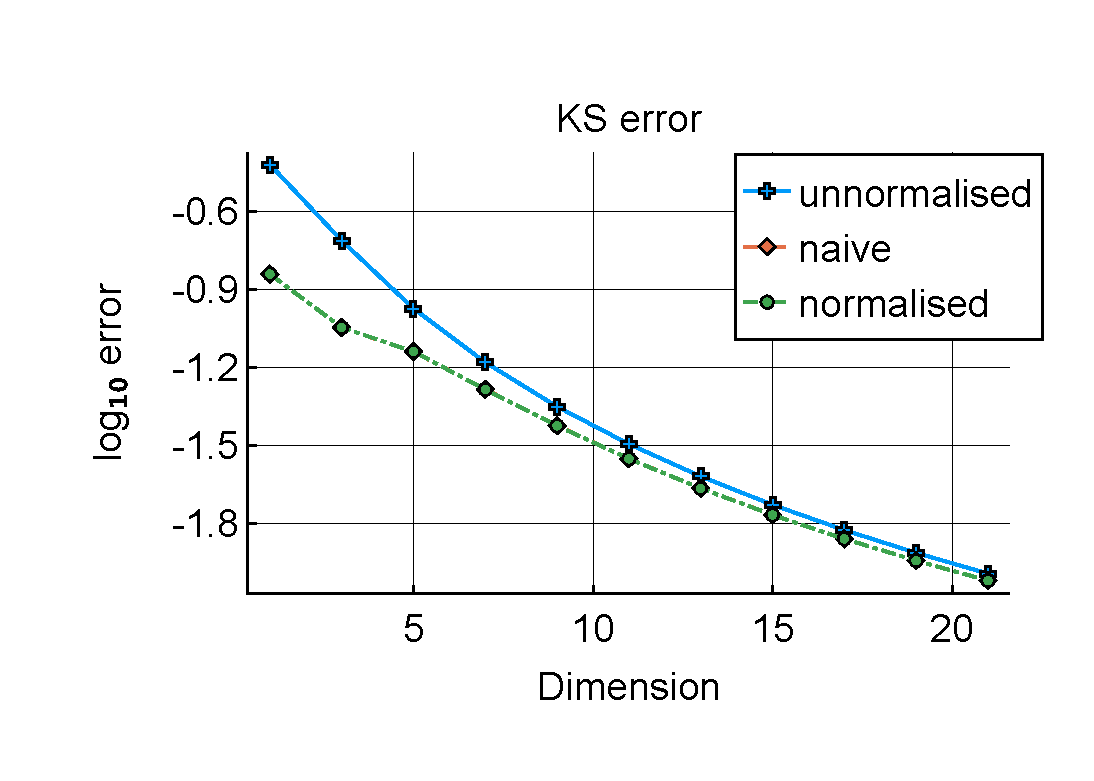
\includegraphics[width=0.5\textwidth,trim={1.25cm 0.8cm 0.25cm 1.25cm},clip]{chapter6/figs/qbdrap_closing_vec/fun6/ks_error_formatted.pdf}%
	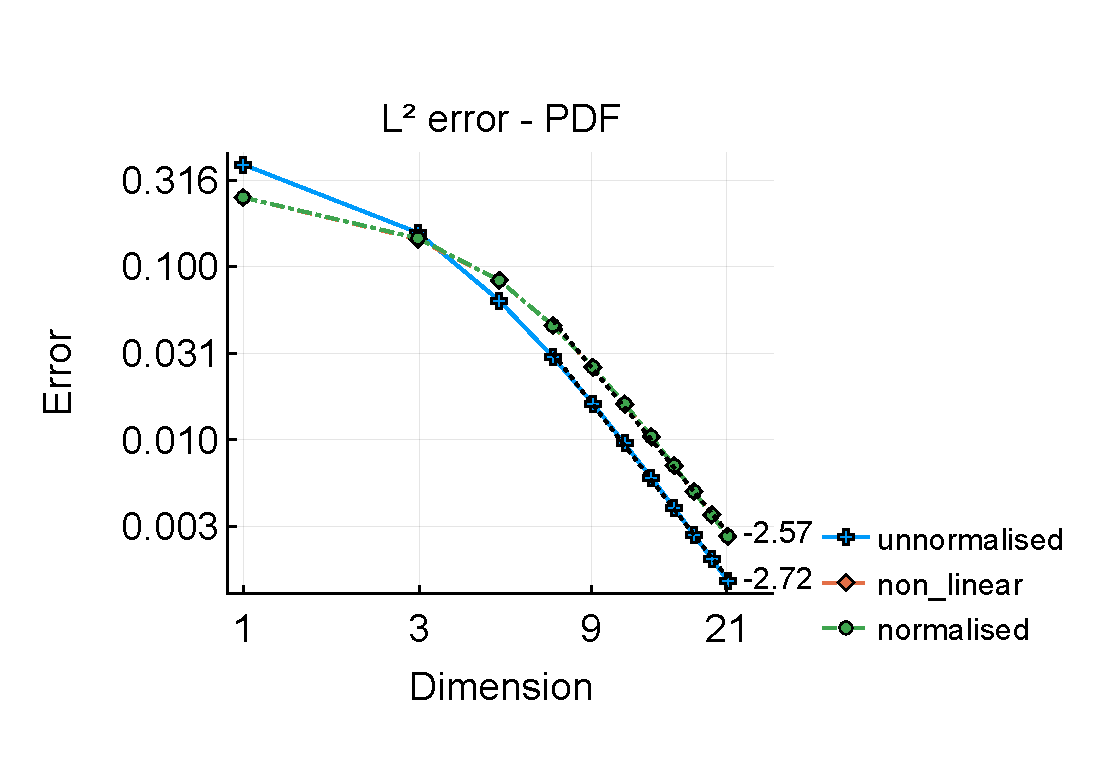
\includegraphics[width=0.5\textwidth,trim={1.25cm 0.8cm 0.25cm 1.25cm},clip]{chapter6/figs/qbdrap_closing_vec/fun6/l2_pdf_error_formatted.pdf}
	\caption{KS error between the true CDF, \(-2x^3+3x^2\), and the approximation (left) and \(L^2\) error between the true PDF \(-6x^2+6x\) and the approximation (right), for the three closing vectors considered; unnormalised (blue solid line with crosses), naive normalised (orange dashed line with diamonds) and normalised (green dash-dotted line with circles). The naive normalised (orange) an normalised closing vectors are coincident.}
	\label{fig: fun 6 ks error qbdrap closing vecs}
\end{figure}

The fact that the unnormalised closing operator outperforms the two normalised ones can be explain, once again, by the fact that, for the normalised operators we have `folded' the ME density function back on itself. In Figure~\ref{fig: pdf reconstructed quadratic} we plot the unnormalised and normalised reconstructions along with the true PDF, \(-6x^2+6x\). In Figure~\ref{fig: pdf reconstructed quadratic} we observe that, at the left of the plot, the normalised reconstructions over estimate the density function in this region, where as the unnormalised reconstruction looks to be doing better. Recall that the `folding' in the normalised closing operator manifest itself as extra mass at the left of these plots compared to the unnormalised reconstructions. 
\begin{figure}
	\centering
	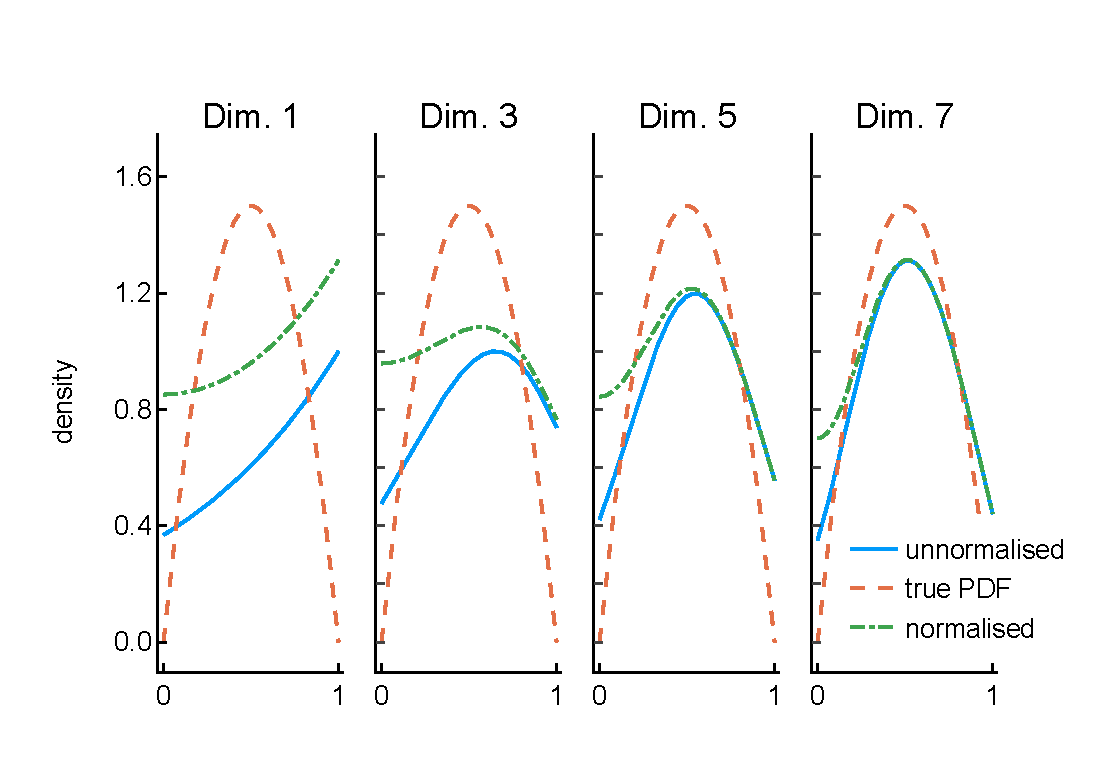
\includegraphics[width=\textwidth]{chapter6/figs/qbdrap_closing_vec/fun6/pdfs_formatted.pdf}
	\caption{Reconstructed PDFs using the unnormalised closing operator (blue solid line), normalised closing operator (green dash-dotted line), for various orders, and the true PDF which is \(f(x)=-6x^2+6x\) (orange dashed line).}
	\label{fig: pdf reconstructed quadratic}
\end{figure} 
\end{example}

\begin{example}Lastly, we consider approximating the initial distribution with PDF \(3e^{-3x}/(1-e^{-3})\). This density function is at a maximum at the left of the region. Considering what we have learnt so far about the unnormalised operator underestimating in this region, we expect that the unnormalised closing operator will perform relatively poorly in this case. Indeed, observing Figures~\ref{fig: fun 7 ks error qbdrap closing vecs} we see that the normalised reconstructions perform relatively well compared to the unnormalised reconstruction as measured by both error metrics (KS statistic and \(L^2\) norm on the PDF). If we observed plots of the PDFs (omitted), we would once again see that this is due to the loss of mass at the left-hand side of the region due to the truncation. 
\begin{figure}
	\centering
	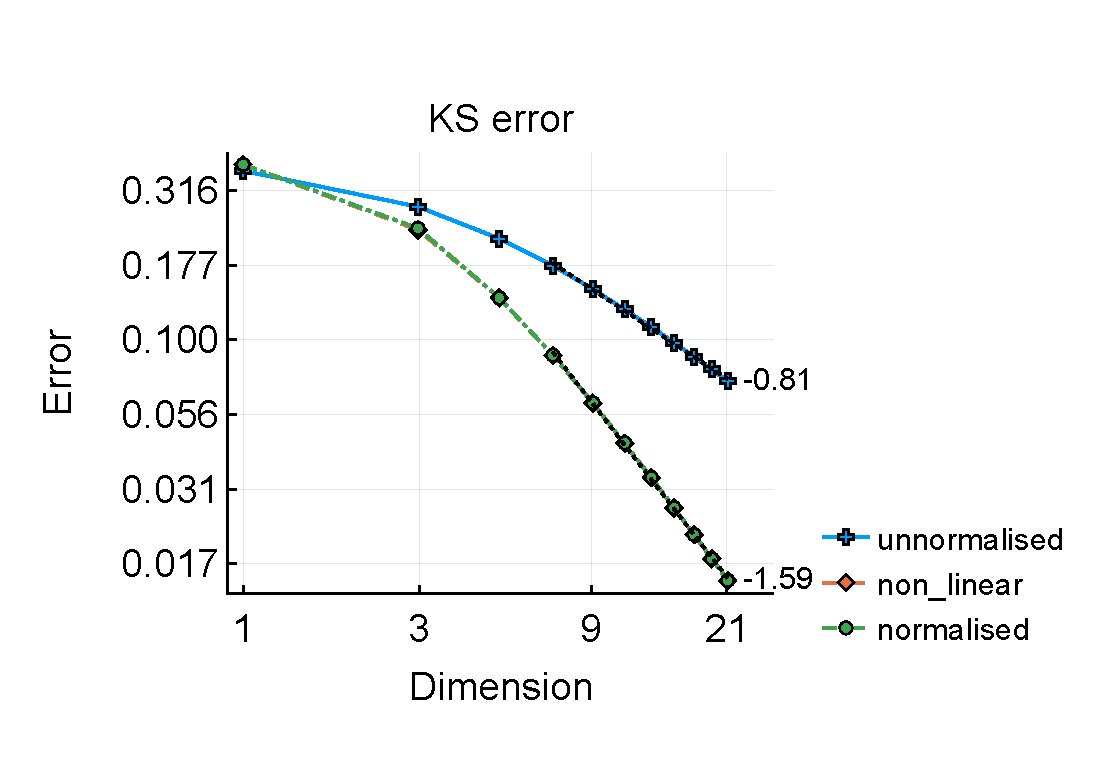
\includegraphics[width=0.5\textwidth,trim={1.25cm 0.8cm 0.25cm 1.25cm},clip]{chapter6/figs/qbdrap_closing_vec/fun7/ks_error_formatted.pdf}%
	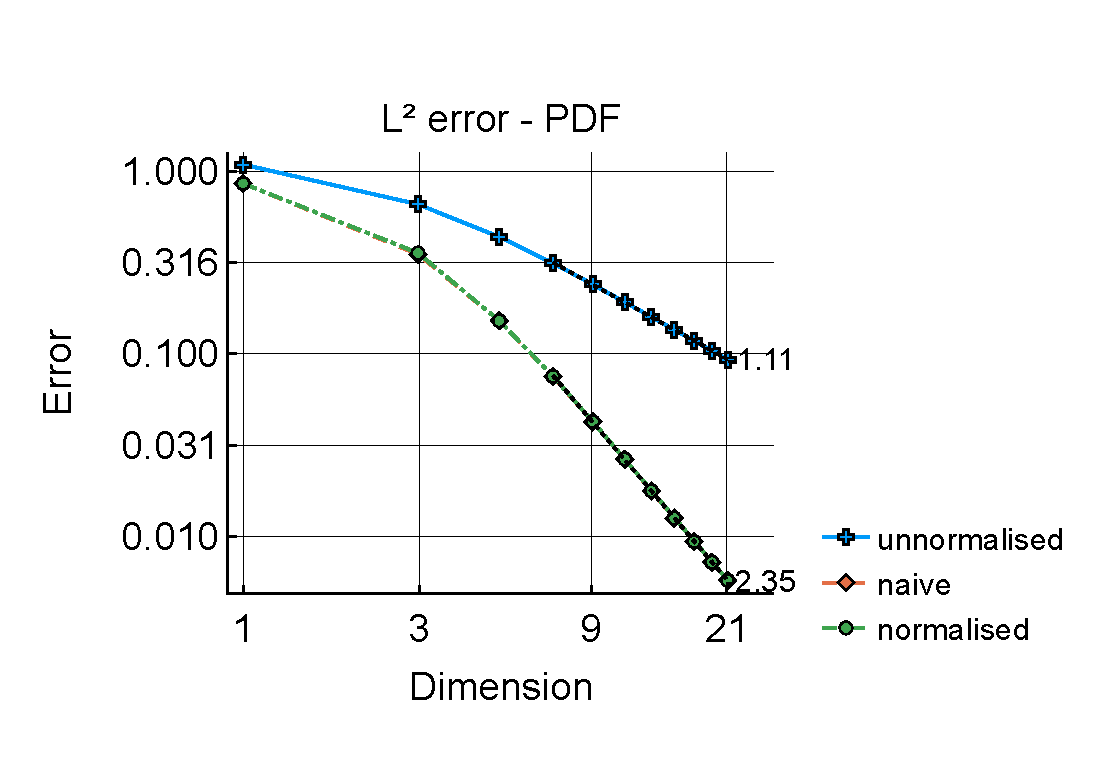
\includegraphics[width=0.5\textwidth,trim={1.25cm 0.8cm 0.25cm 1.25cm},clip]{chapter6/figs/qbdrap_closing_vec/fun7/l2_pdf_error_formatted.pdf}
	\caption{KS error between the true CDF, \((1-e^{-3x})/(1-e^{-3})\), and the approximation (left) and \(L^2\) error between the true PDF and the approximation for the three closing vectors considered; unnormalised (blue solid line with crosses), naive normalised (orange dashed line with diamonds) and normalised (green dash-dotted line with circles). The naive normalised (orange) an normalised closing vectors are coincident.}
	\label{fig: fun 7 ks error qbdrap closing vecs}
\end{figure}
\end{example}

Given the evidence above we choose to use the normalised closing operator to reconstruct solutions. Further, unlike the naive normalised operator, the normalised operator is theoretically justified in that we proved the closing operator leads to a convergent scheme and is linear. 

\subsection{Comparison of methods}\label{sec: comp}
Here we compare the ability of the QBD-RAP, uniformisation, and DG methods to reconstruct initial conditions. 

\begin{example}First we consider the initial condition with CDF \(1(x\geq 0.5)\), that is, a point mass at 0.5. This distribution does not have a PDF so we can compare the CDFs only. In Figure~\ref{fig: fun 1 comp} we plot the KS metric (left) and \(L^1\) metric (right) between the true CDF and the reconstructed approximations. Observing the KS metric, it appears that none of the methods converge and the KS error sits around 0.5. This reflects the fact that convergence in distribution implies point-wise convergence of the CDFs except at points of discontinuity. None of the methods appear to converge at this point. Observing the \(L^1\) error between the true CDF and reconstructed approximation (which is the area between the two CDFs) we now see that the methods appear to show the convergent behaviour we expect. Here, the uniformisation method appears to perform the best, while the QBD-RAP method performs the worst. The rate of convergence of the QBD-RAP method appears to be similar to the rate of convergence of the DG scheme. 

Perhaps it is no surprise that the uniformisation method performs best. In the uniformisation method as we increase the order, we partition the cell \([0,1]\) into smaller sub-cells, and use constant functions on each sub-cell to approximate the function. As such, the uniformisation method can produce a piecewise continuous, linear approximation to the CDF. In contrast, both the DG and QBD-RAP methods result in a smooth approximation to the CDF. 
\begin{figure}
	\centering
	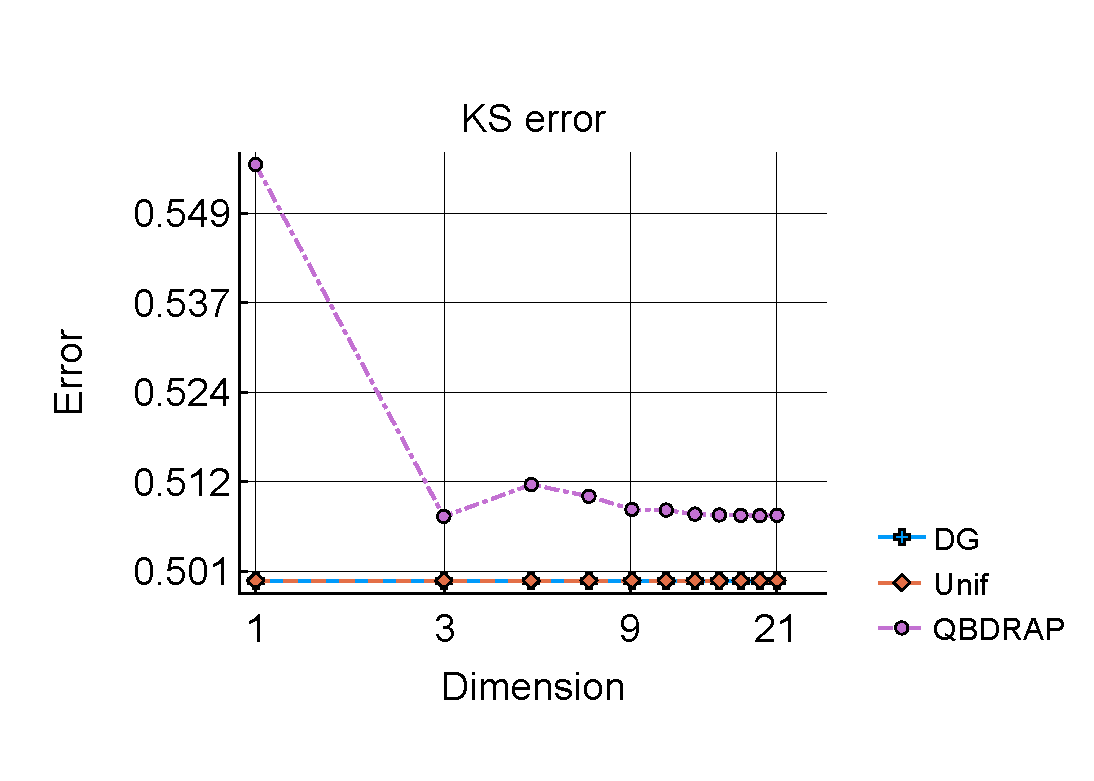
\includegraphics[width=0.5\textwidth,trim={1.25cm 0.8cm 0.25cm 1.25cm},clip]{chapter6/figs/comp/fun1/meshs_ks_error_formatted.pdf}%
	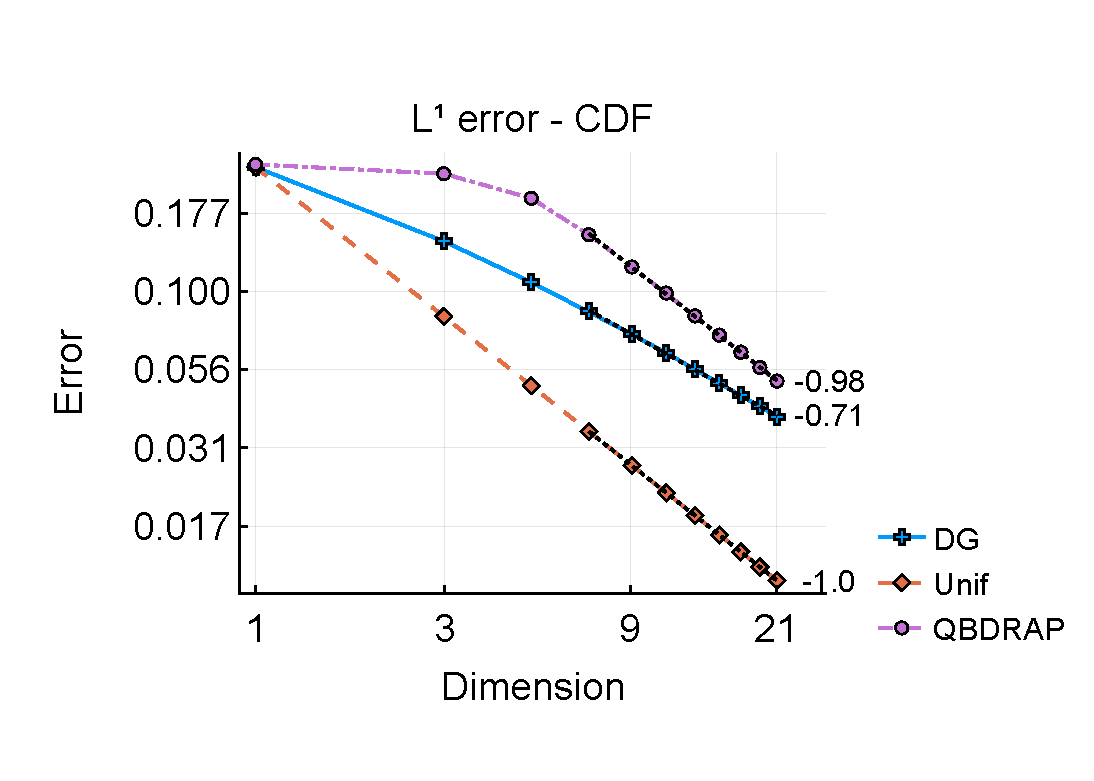
\includegraphics[width=0.5\textwidth,trim={1.25cm 0.8cm 0.25cm 1.25cm},clip]{chapter6/figs/comp/fun1/meshs_l1_cdf_error_formatted.pdf}
	\caption{KS error between the true CDF, \(1(x\geq 0.5)\), and the approximations (left) and \(L^1\) error between the true CDF and the approximations for the DG method (blue solid line with crosses), uniformisation method (orange dashed line with diamonds) and QBD-RAP method (green dash-dotted line with circles).}
	\label{fig: fun 1 comp} 
\end{figure}

In Figure~\ref{fig: pdf comp fun 1} we plot the approximated CDFs for the DG, uniformisation and QBD-RAP methods alongside the true CDF. The DG method displays undesirable features for an approximation to a CDF -- it is not monotonically increasing, at some points it is negative and at some points it is above 1. On the other hand, although the QBD-RAP method converges slowest, it displays good properties in that it results in a monotonically increasing CDF, starting at 0 and ending at 1. 
\begin{figure}
	\centering
	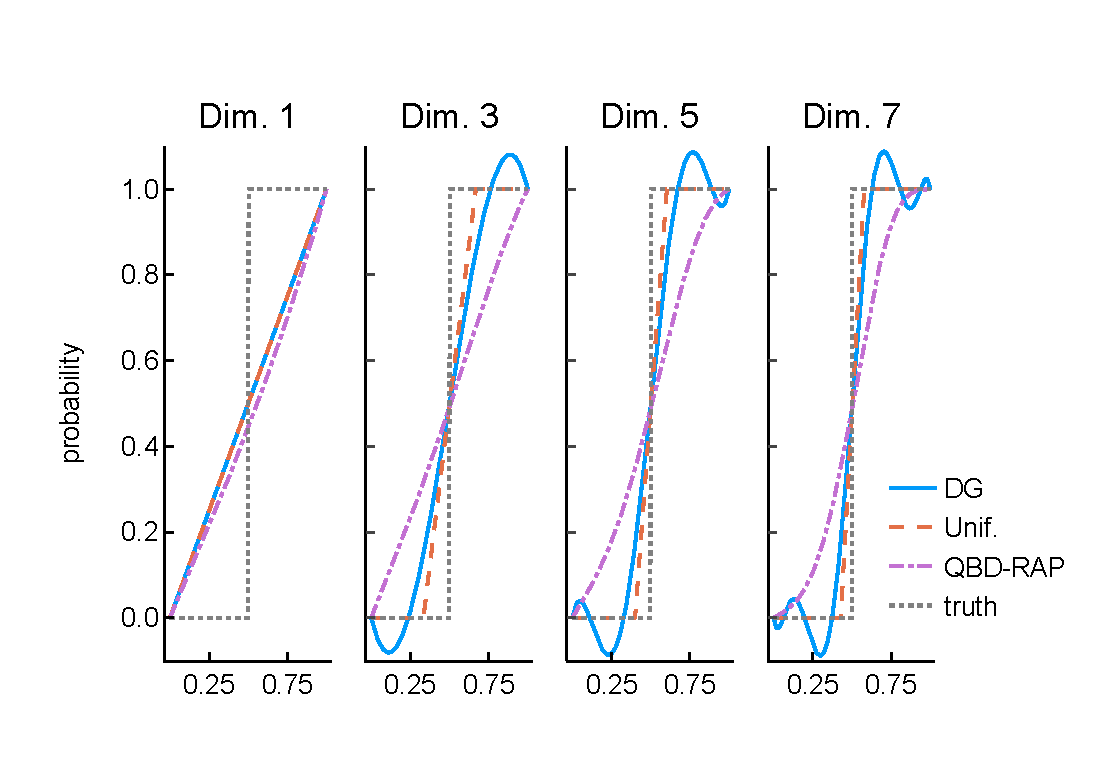
\includegraphics[width=\textwidth]{chapter6/figs/comp/fun1/cdfs_formatted.pdf}
	\caption{Reconstructed CDFs using the DG (blue solid line), uniformisation (orange dashed line) and QBD-RAP (green dot-dashed line) methods. The true distribution function is \(1(x\geq 0.5)\) (grey dotted line).}
	\label{fig: pdf comp fun 1}
\end{figure} 
\end{example}

\begin{example}Now consider approximating the initial distribution with PDF \(1(x\leq 0.5)\). Figure~\ref{fig: fun 2 comp} plots the KS error (left) and \(L^2\) error between the true and approximate PDFs (right). Figure~\ref{fig: fun 2 comp} suggests that all methods converge at a similar rate for this problem. Once again, the QBD-RAP method performs worst, the uniformisation method second, and the DG method the best. However, once again the DG method exhibits undesirable properties -- the approximation to the CDF is, at some points above 1, is not monotonic, though these violations are not as severe in this case as they were for the case above. 
\begin{figure}
	\centering
	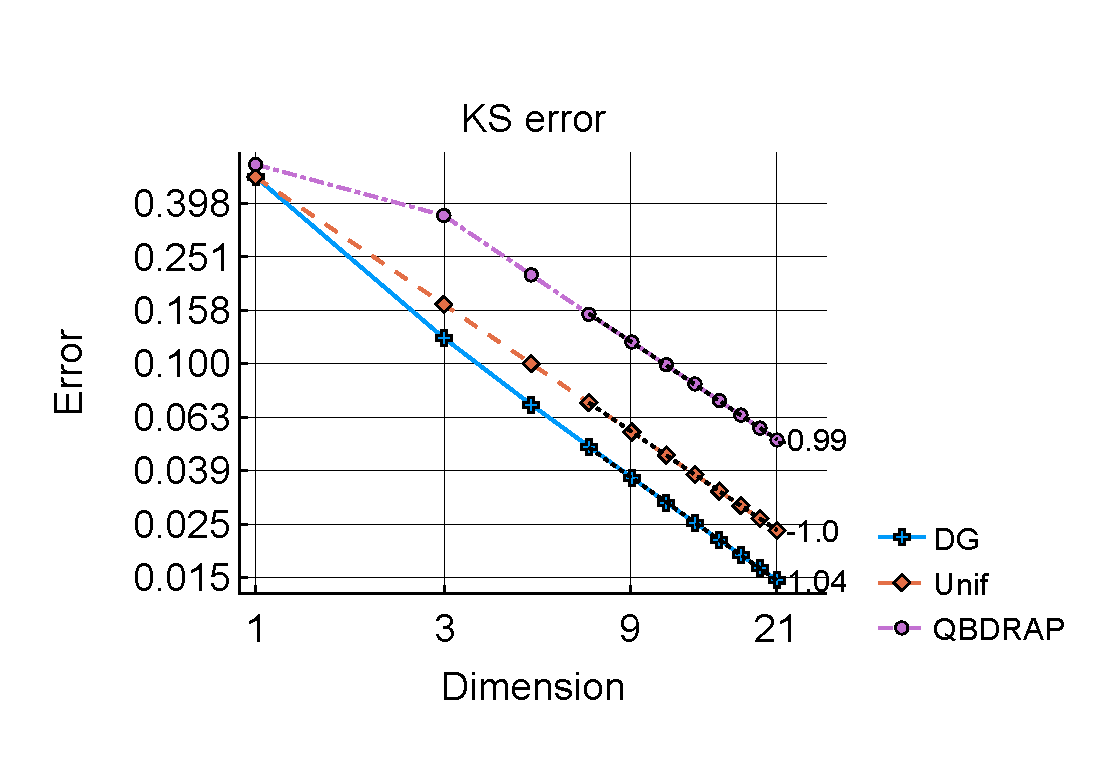
\includegraphics[width=0.5\textwidth,trim={1.25cm 0.8cm 0.25cm 1.25cm},clip]{chapter6/figs/comp/fun2/meshs_ks_error_formatted.pdf}%
	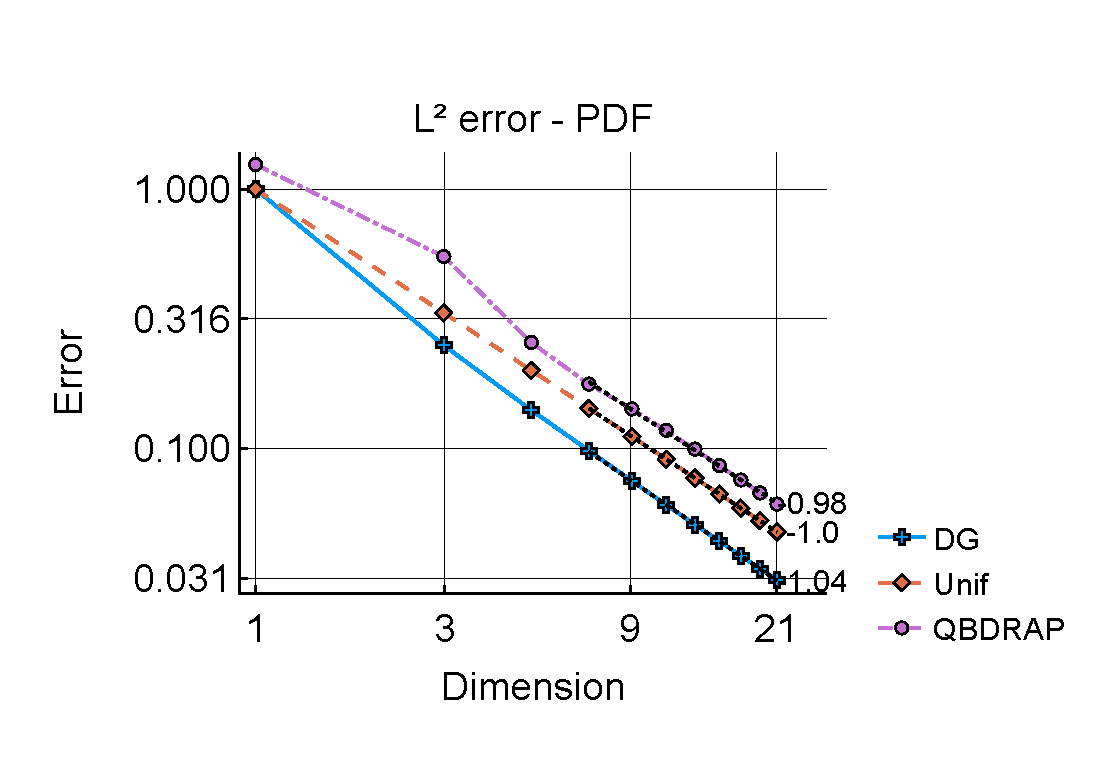
\includegraphics[width=0.5\textwidth,trim={1.25cm 0.8cm 0.25cm 1.25cm},clip]{chapter6/figs/comp/fun2/meshs_l2_pdf_error_formatted.pdf}
	\caption{KS error between the true CDF and the approximations (left) and \(L^2\) error between the true PDF, \(1(x\geq 0.5)\), and the approximations for the DG method (blue solid line with crosses), uniformisation method (orange dashed line with diamonds) and QBD-RAP method (green dash-dotted line with circles).}
	\label{fig: fun 2 comp} 
\end{figure}
\end{example}

\begin{example}So far we have considered two problems which exhibit discontinuities. At the other extreme we now consider an initial distribution with density \(-6z^2+6x\). In Figure~\ref{fig: fun 6 comp} we plot the KS error and the \(L^2\) error between the true and approximated PDF. Since the DG method projects the initial condition onto a polynomial basis, then, for an order 3 approximation and above, the DG method can theoretically approximate the initial condition exactly. This is reflected in Figure~\ref{fig: fun 6 comp}, where the blue curve drops sharply from 1-3, then plateaus. Due to numerical integration errors, for example in the evaluation of the integral in the \(L^2\) norm, and due to machine arithmetic, the errors for the DG scheme are not 0. Regarding the other two methods, they too appear to be convergent at approximately the same rate, with the uniformisation method perform better for the KS error, but very similarly in terms of the \(L^2\) error. 
\begin{figure}
	\centering
	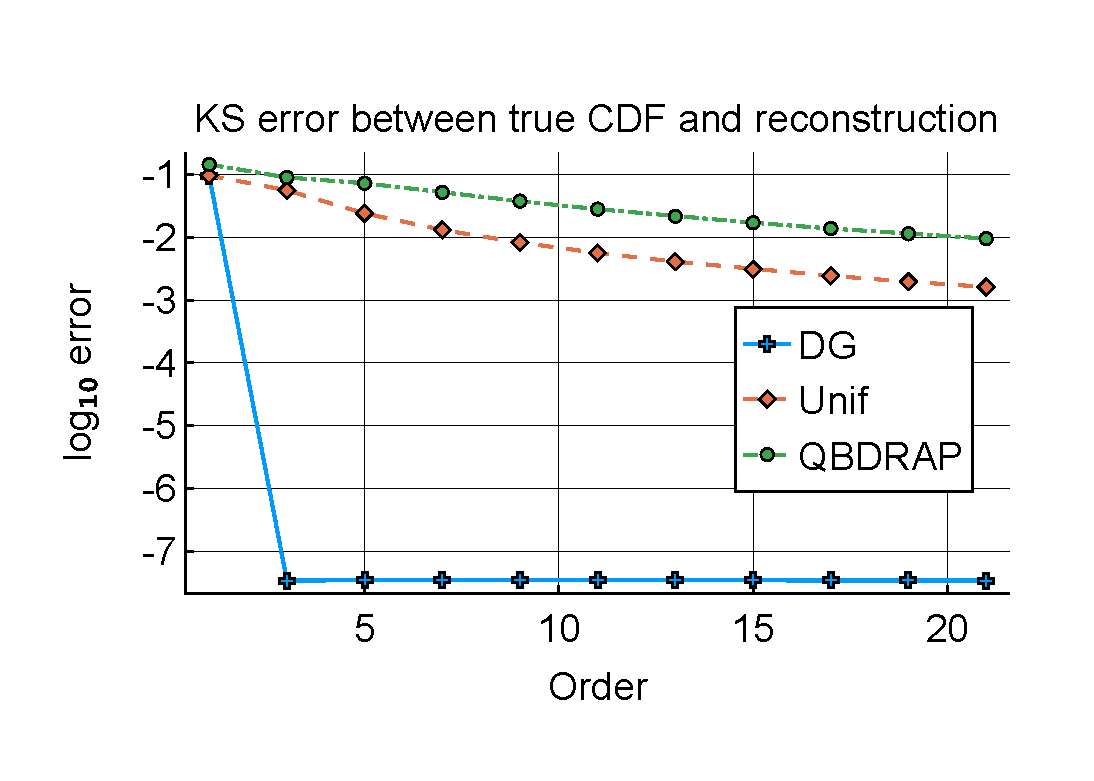
\includegraphics[width=0.5\textwidth,trim={1.25cm 0.8cm 0.25cm 1.25cm},clip]{chapter6/figs/comp/fun6/meshs_ks_error_formatted.pdf}%
	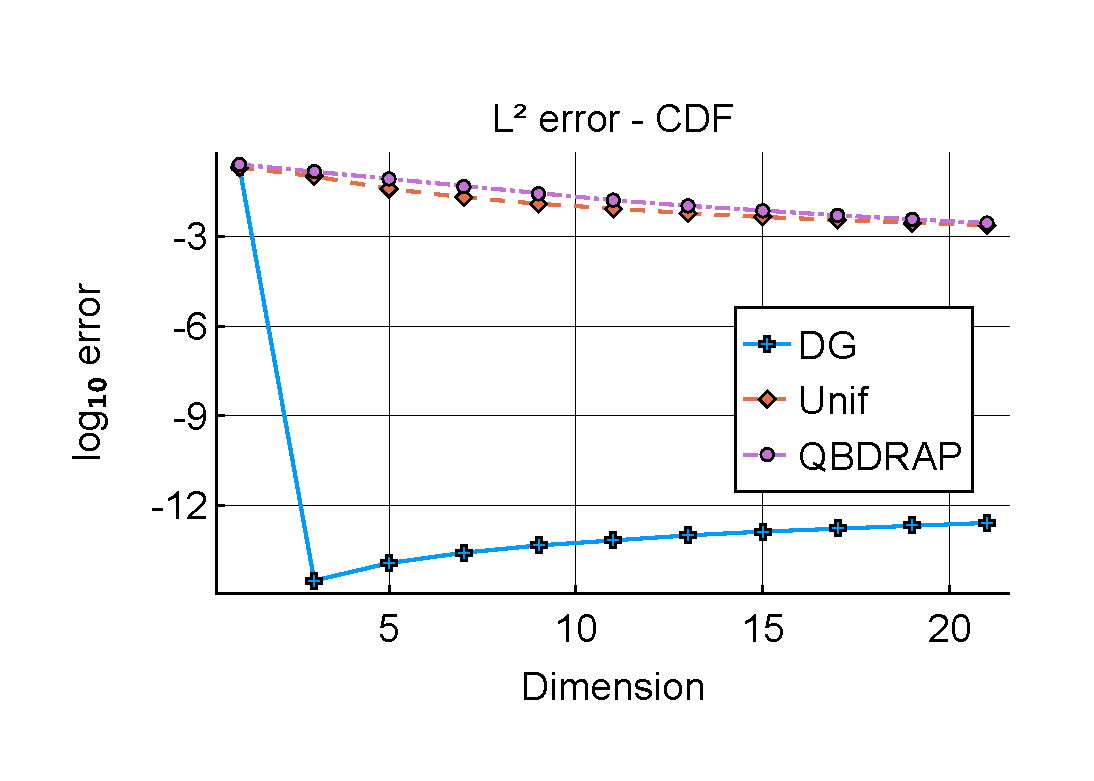
\includegraphics[width=0.5\textwidth,trim={1.25cm 0.8cm 0.25cm 1.25cm},clip]{chapter6/figs/comp/fun6/meshs_l2_pdf_error_formatted.pdf}
	\caption{KS error between the true CDF and the approximations (left) and \(L^2\) error between the true PDF, \(-6z^2+6x\), and the approximations for the DG method (blue solid line with crosses), uniformisation method (orange dashed line with diamonds) and QBD-RAP method (green dash-dotted line with circles).}
	\label{fig: fun 6 comp} 
\end{figure}
\end{example}

\begin{example}Consider now the initial distribution with PDF \(cos(4\pi(x+0.5))+1\). Figure~\ref{fig: fun 9 comp} shows the errors. Both the KS error (left) and \(L^2\) norm between the true and approximated PDFs tell a similar story. For sufficiently high order, the DG method approximates the inital condition very well. The uniformisation method performs second best, while the QBD-RAP method is slowest to converge. 
\begin{figure}
	\centering
	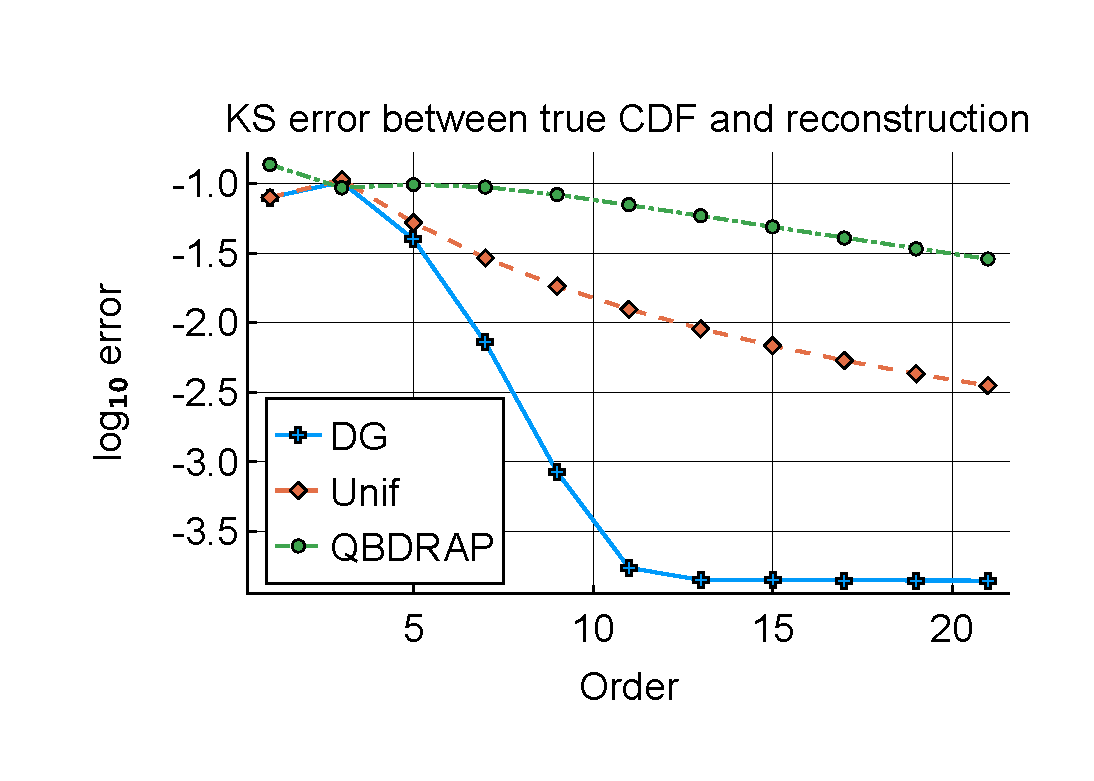
\includegraphics[width=0.5\textwidth,trim={1.25cm 0.8cm 0.25cm 1.25cm},clip]{chapter6/figs/comp/fun9/meshs_ks_error_formatted.pdf}%
	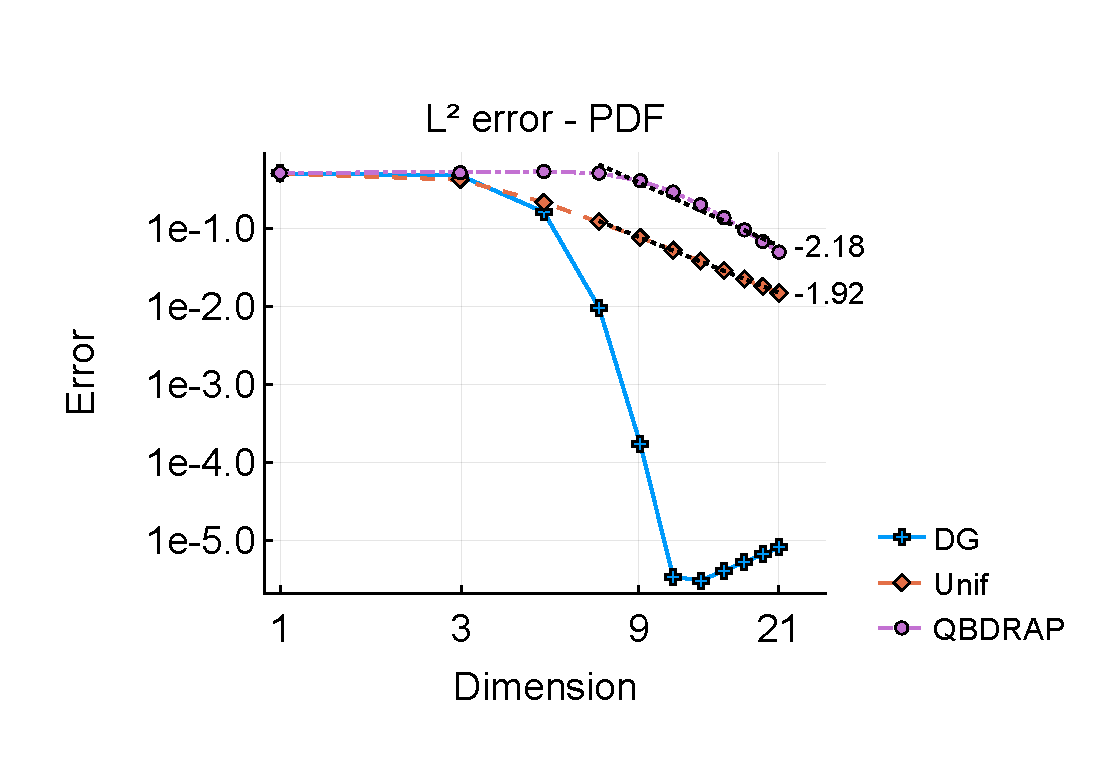
\includegraphics[width=0.5\textwidth,trim={1.25cm 0.8cm 0.25cm 1.25cm},clip]{chapter6/figs/comp/fun9/meshs_l2_pdf_error_formatted.pdf}
	\caption{KS error between the true CDF and the approximations (left) and \(L^2\) error between the true PDF, \(cos(4\pi(x+0.5))+1\), and the approximations for the DG method (blue solid line with crosses), uniformisation method (orange dashed line with diamonds) and QBD-RAP method (green dash-dotted line with circles).}
	\label{fig: fun 9 comp} 
\end{figure}
\end{example}
\FloatBarrier

\section{Travelling wave}
Here we investigate the performance the different schemes for approximating transient distributions of one-dimensional travelling wave problems with varying initial conditions. Consider a (trivial) fluid queue with one phase, generator \(\bs T=[0]\) and rate \(c=1\). The PDE (if/when it exists) which describes this system is 
\[\cfrac{\partial}{\partial t} f(x,t) = -\cfrac{\partial}{\partial x} f(x,t),\]
where \(f(x,t)\) is the density at time \(t\). Given an initial condition, \(f(x,0)\), solutions to this problem are given by 
\[f(x,t) = f(x-t,0)\]
so the solution at time \(t\) is just a shift in the initial condition \(t\) units to the right. We suppose that the fluid queue is bounded, with a lower boundary \(x=0\) and upper boundary \(x=10\). 

We use the QBD-RAP, uniformisation and DG schemes to discretise the solution in space. We discretise the interval \([0,10]\) into \(10\) cell, each of width 1. We use \(10,001\) points to approximate the integrals which appear in the construction of the initial conditions, to approximate the integrals appearing in the error metrics, and also as a set of discrete points on which evaluate the CDFs to approximate the KS metric. We use the SSPRK4 method to integrate over time using a step size of \(0.005\), and we evolve the system until time \(t=4\). For the DG method we also implement the Generalise MUSCL (REF, appendix?) slope limiter to stabilise the integration. 

\begin{example}First consider the initial condition with PDF \(1(x<1)\). The level of the fluid queue is uniformly distributed over the first cell. For the DG and uniformisation methods, the initial condition can be represented exactly, whereas, for the QBD-RAP method, it cannot. Thus, in this case, there is no discretisation error in constructing the initial condition for the DG and uniformisation methods. Furthermore, at time \(t=4\), the solution in \(1(x\in[4,5)\), and the projections related to the DG and uniformisation methods can represent this solution exactly too.

Figure~\ref{fig: fun 4 wave} plots the KS error between the approximated and true CDFs and \(L^2\) error between the approximated and true PDFs. The DG method with the MUSCL limiter does not appear to converge for this problem. This is caused by the limiter reducing the method to linear in when oscilations are deteced, so increasing the order does not increase the accuracy of the method. The other two positivity preserving methods, the uniformisation method and QBD-RAP methods, both appear to be converging, with the QBD-RAP method converging faster. With these error metrics, the DG method also appears to converge. However, if we observe the solutions resulting from the DG method (Figure~\ref{fig: pdf wave fun 4} top-row), we find them to be unsatisfactory due to oscilations and negative values. 

Figure~\ref{fig: pdf wave fun 4} plots the density functions reconstructed using the DG, uniformisation, DG with MUSCL limiter and QBD-RAP methods. In the first row we observe that the DG method (sans limiter) produces an approximation to the PDF with negative values for orders greater than 1. In the third row of Figure~\ref{fig: pdf wave fun 4} we observe that, with the limiter the approximation does not change significantly after order 3. This is due the the fact that the DG method is at best linear. In the second row of Figure~\ref{fig: pdf wave fun 4} is the solution approximated using the uniformisation method, and in the last row is the solution approximated using the QBD-RAP method. 
\begin{figure}
	\centering
	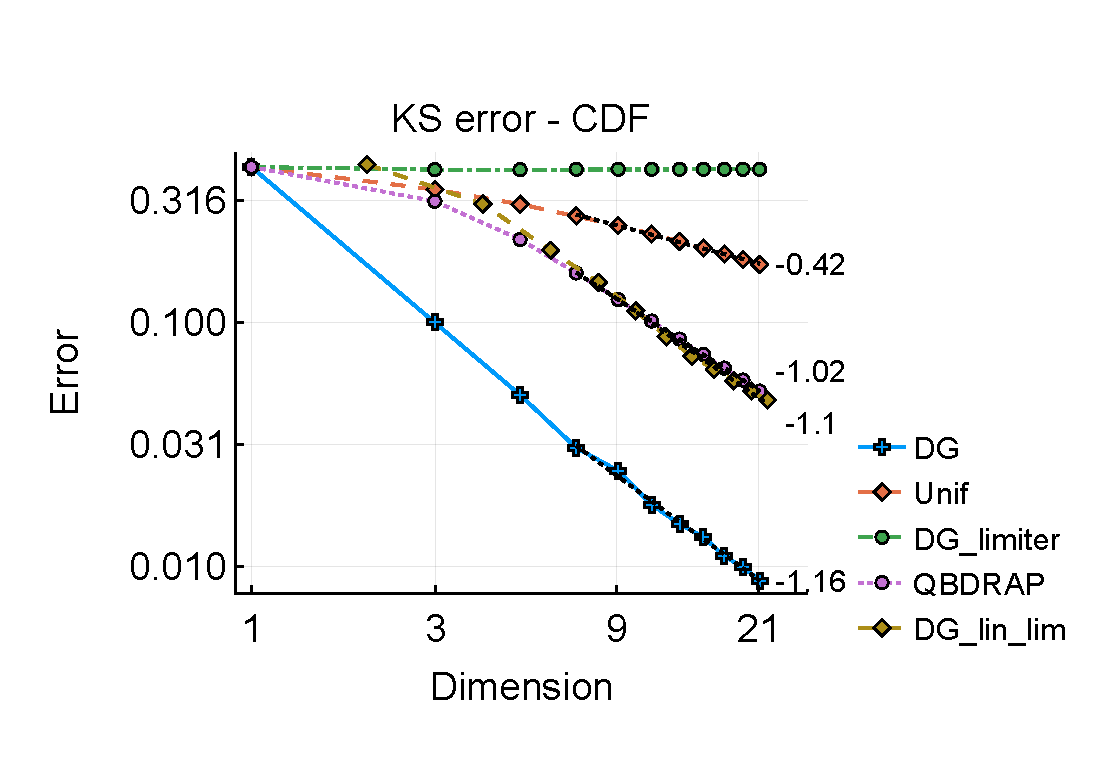
\includegraphics[width=0.5\textwidth,trim={0.75cm 0.8cm 0.25cm 1.25cm},clip]{chapter6/figs/wave/fun4/meshs_ks_error_formatted.pdf}%
	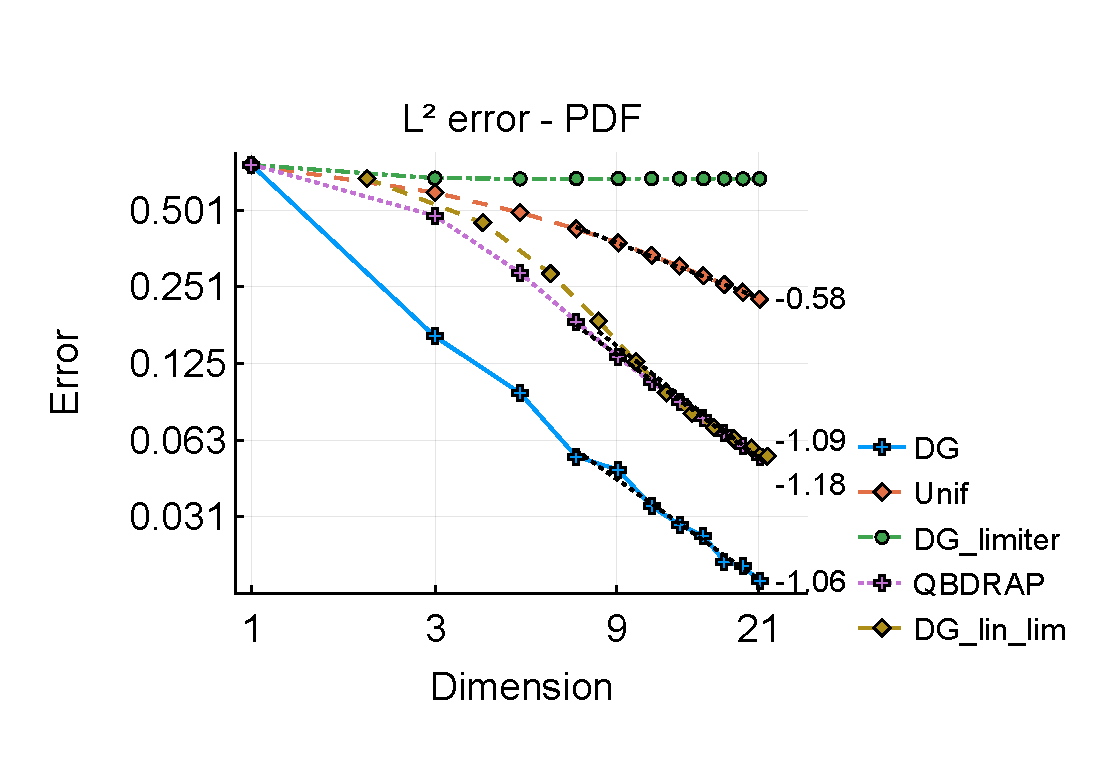
\includegraphics[width=0.5\textwidth,trim={0.75cm 0.8cm 0.25cm 1.25cm},clip]{chapter6/figs/wave/fun4/meshs_l2_pdf_error_formatted.pdf}
	\caption{KS error between the true CDF and the approximations (left) and \(L^2\) error between the true PDF, \(1(4\leq x < 5)\), and the approximations for the DG method (blue solid line with crosses), DG method with the MUSCL limiter (green dash-dotted line with crosses), uniformisation method (orange dashed line with diamonds) and QBD-RAP method (green dash-dotted line with circles).} 
	\label{fig: fun 4 wave} 
\end{figure}
\begin{figure}
	\centering
	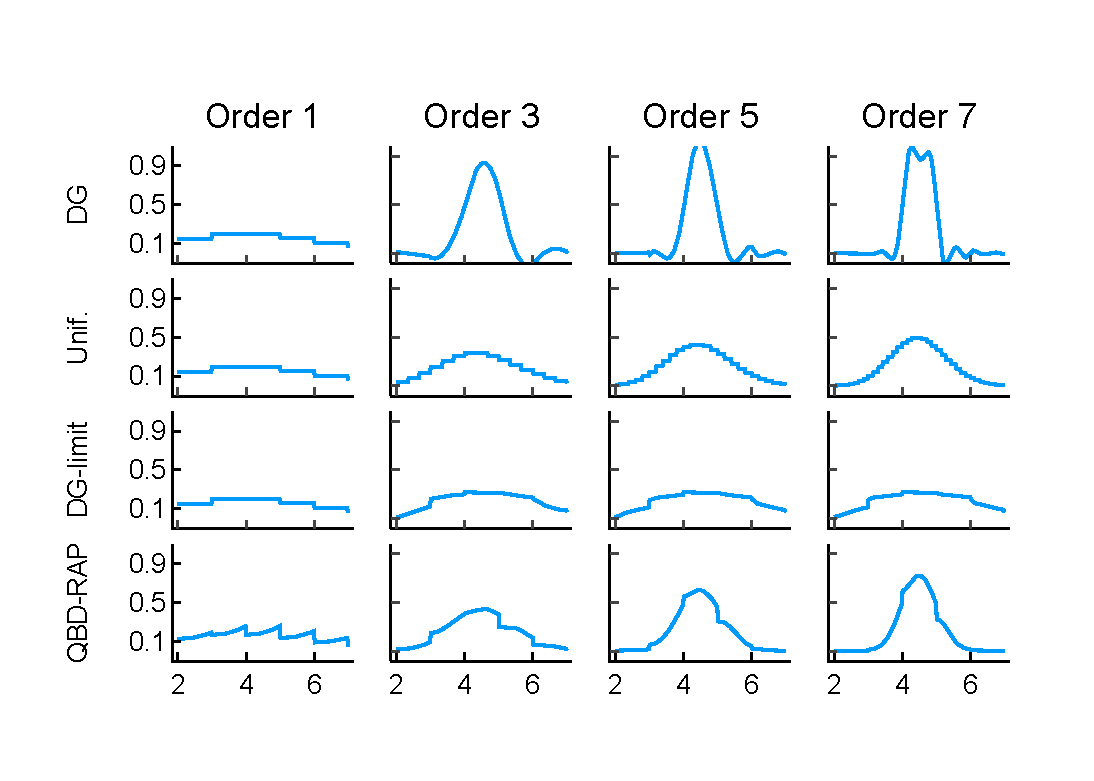
\includegraphics[width=\textwidth]{chapter6/figs/wave/fun4/pdfs_formatted.pdf}
	\caption{Reconstructed PDFs using the DG (top row), uniformisation (second row), DG with MUSCL limiter (third row) and QBD-RAP (bottom row) methods, for order 1, 3, 5, and 7 (columns). The true density function is \(1(4\leq x<5)\).}
	\label{fig: pdf wave fun 4}
\end{figure} 

This is a particularly interesting example. It shows that, for the DG method, even though there is no discretisation error for the initial condition, we have use a strong stability preserving time-intergration method, and the projection off which the DG method is based can represent the transient distribution at time \(t=4\) exactly, there is still the possibility of badly behaved solutions as in the top row of Figure~\ref{fig: pdf wave fun 4}. 
\end{example}

\begin{example}Another interesting example occurs with the initial condition with CDF \(1(z\geq 0.5)\), i.e.~a point mass at 0.5. The exact solution at time \(t=4\) is therefore a point mass at \(4.5\). No PDF exists for the true distribution, so instead we compare the CDFs. Moreover, when we analysed reconstruction of this initial condition we saw that using the KS metric may be uninformative. Instead, for this example, we measure errors by looking at the \(L^1\) error between the CDFs (the area between the CDFs). We also compare the probabilities
\begin{align}
	\mathbb P(X(4)\in\calD_{\ell,1}, \varphi(4)=1\mid X(0)=0.5,\varphi(0)=1) \label{eqn: cell probs}
\end{align}
for \(\ell=1,\dots,K\), and also the boundary mass
\begin{align}
	\mathbb P(X(4)\in\{10\}, \varphi(4)=1\mid X(0)=0.5,\varphi(0)=1) \label{eqn: cell probs boundary}
\end{align}
by computing 
\begin{align}
	&\sum_{\ell=1}^{10} \left|\mathbb P(X(4)\in\calD_{\ell,1}, \varphi(4)=1\mid X(0)=0.5,\varphi(0)=1)-p(4,\ell,1)\right|\nonumber 
	\\&+\left|\mathbb P(X(4)\in\{10\}, \varphi(4)=1\mid X(0)=0.5,\varphi(0)=1)-p(4,11,1)\right| \label{eqn: cell errors}
\end{align}
where \(p(4,\ell,1)\) is an approximation to \(\mathbb P(X(4)\in\calD_{\ell,1}, \varphi(4)=1\mid X(0)=0.5,\varphi(0)=1)\), and \(p(4,11,1)\) is an approximation to \(\mathbb P(X(4)\in\{10\}, \varphi(4)=1\mid X(0)=0.5,\varphi(0)=1)\).

Figure~\ref{fig: fun 2 wave} (left) plots the \(L^1\) error between the true and approximated CDFs (left). The \(L^1\) metric tells a similar story to the previous analysis: the DG method with the limiter does not converge as order increases, the other two positivity preserving methods, the uniformisation and QBD-RAP methods, appear to converge, with the QBD-RAP method converging faster, while the DG method appears to converge the fastest. However, if we plot the approximations to the CDFs from the DG method (not shown) we would once again see an oscilating non-monotonic approximation. Another interesting observation is to compare the performance of the uniformisation and QBD-RAP methods with respect to the \(L^1\) metric on the CDFs in Figure~\ref{fig: fun 2 wave} (left) to that in Figure~\ref{fig: fun 1 comp} (right). Recall that with Figure~\ref{fig: fun 1 comp} we investigate the ability of the different approximation methods to represent the initial distribution with CDF \(1(x\geq 1)\), which is the initial condition of the problem we are consdiering here. In Figure~\ref{fig: fun 1 comp} (right) the uniformisation method out-performed the QBD-RAP method at reconstructing the inital condition. However, in Figure~\ref{fig: fun 2 wave} (left) we see that the QBD-RAP method out-performs the uniformisation method. This suggest that the QBD-RAP method is better able to resolve movement of mass across the domain when integrating over time, compared to the uniformisation method.  

Figure~\ref{fig: fun 2 wave} (right) plots the cell-based error metric in (\ref{eqn: cell errors}). Once again, the DG method with MUSCL limiter does not appear to converge as we expect. The uniformisation and QBD-RAP method both appear to converge, with the QBD-RAP method converging faster. Most interestingly though is the DG method. It is unclear as to whether this method will converge in this case as the errors in the plot are not obviously decreasing. Moreover, with this metric, the QBD-RAP method out-performs the DG method. Furthermore, the DG method can result in negative estimates of the cell probabilities in (\ref{eqn: cell probs}) and (\ref{eqn: cell probs boundary})
\begin{figure}
	\centering
	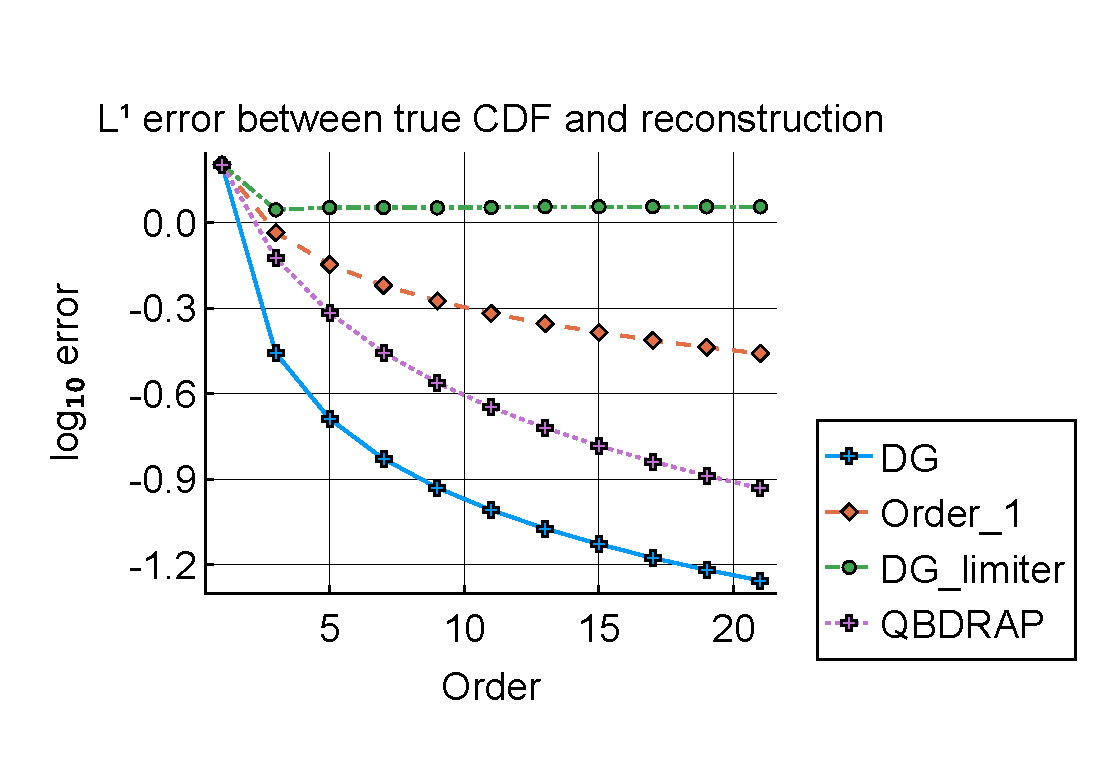
\includegraphics[width=0.5\textwidth,trim={0.75cm 0.8cm 0.25cm 1.25cm},clip]{chapter6/figs/wave/fun2/meshs_l1_cdf_error_formatted.pdf}%
	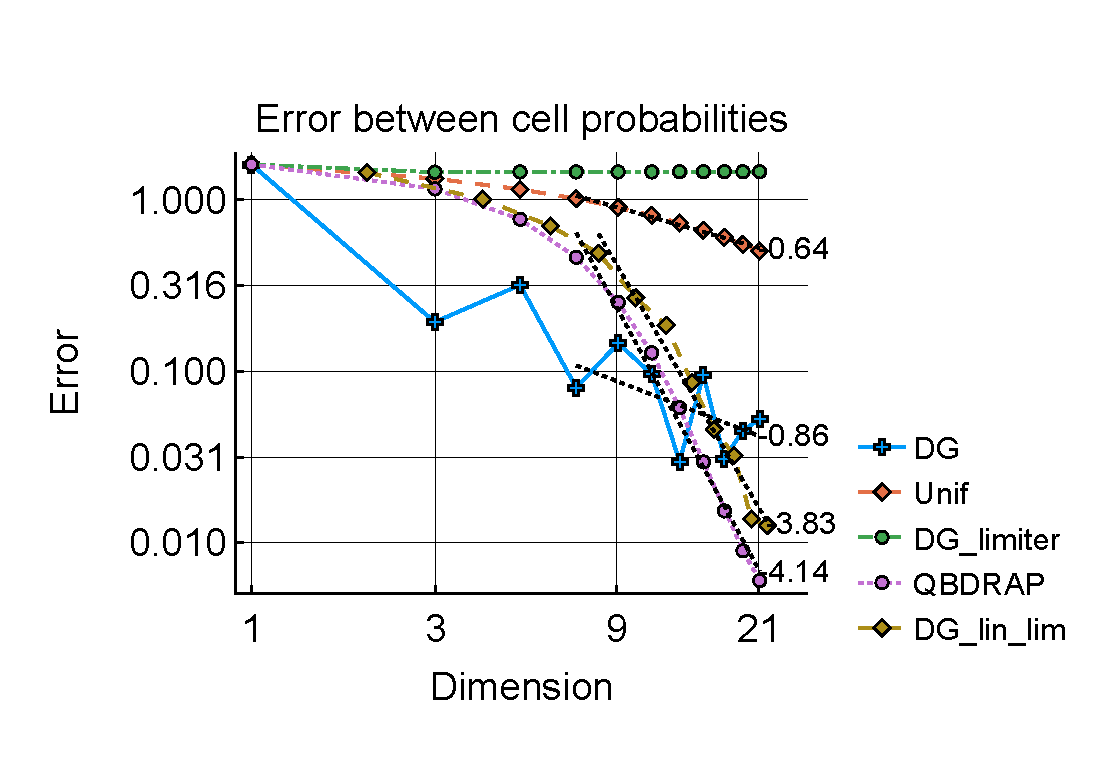
\includegraphics[width=0.5\textwidth,trim={0.75cm 0.8cm 0.25cm 1.25cm},clip]{chapter6/figs/wave/fun2/L1_cell_probs.pdf}
	\caption{\(L^1\) error between the true CDF, \(1(4.5\leq x)\), and the approximations (left) and the error metric based on the cell masses as described in (\ref{eqn: cell errors}) for the DG method (blue solid line with crosses), DG method with the MUSCL limiter (green dash-dotted line with crosses), uniformisation method (orange dashed line with diamonds) and QBD-RAP method (green dash-dotted line with circles).} 
	\label{fig: fun 2 wave} 
\end{figure}
\end{example}

\begin{example}
	Now consider an initial distribution which is truncated Gaussian with mean parameter 2.5 and standard deviation parameter 0.5, and trucated at the boundaries, 0 and 10;
	\begin{align}
		\mu([0,x)) := \mathbb P(X(0)\leq x, \varphi(0)=1)=\cfrac{\Phi((x-2.5)/0.5)1(0 \leq x < 10.0)}{\Phi(7.5/0.5)-\Phi(-2.5/0.5)} + 1(10\leq x), \label{eqn: kdjfksdf}
	\end{align}
	where \(\Phi(x)\) is the CDF of the standard normal distribution.

	Hence, at time \(t=4\) the distribution is truncated Gaussian with mean parameter 6.5, standard deviation parameter 0.5, and is truncated below at 4.0 and above at 10, and there is also a small mass at the upper boundary; 
	\begin{align}
		&\mathbb P(X(4)\leq x, \varphi(4)=1\mid X(0)\sim\mu, \varphi(0)=1) \nonumber 
		\\&=\cfrac{\Phi((x-6.5)/0.5)1(4.0\leq x)}{\Phi(7.5/0.5)-\Phi(-2.5/0.5)} + 1(10 \leq x)\label{eqn: bbbbbaabbaa}%\cfrac{\Phi(7.5/0.5)-\Phi(3.5/0.5)}{\Phi(7.5/0.5)-\Phi(-2.5/0.5)}.
	\end{align}
	The mass at the boundary is approximately \(1.28\times 10^{-12}\). There is a small discontinuity at \(x=4\) where the CDF jumps from \(0\) to \(\approx 2.87\times 10^{-7}\), due to the truncation of the initial distribution at \(0\). 

	Since the discontinuity at \(x=4\) is small (much smaller than numerical integration errors in the evaluation of the error metrics), and the distribution is otherwise smooth, we expect that the DG method will perform well for this example. Figure~\ref{fig: fun 6 wave} confirms that this is indeed the case. For both metrics the error obtained by the DG method rapidly decreases to a point where it is swamped by other numerical errors. This is charaterisitc of the DG method for smooth problems. For low order DG schemes there are regions where the approximated PDF is negative, however, as the order of the DG scheme increases, these regions dissipate. Interestingly, even though this is a relatively smooth problem, the DG method with MUSCL limiter does not perform well. It must be that the initial and transient distributions are sufficiently `pointy' that small oscillations in the numerical solutions occur, and the limiter reduces the order of the scheme to linear. Both the uniformisation and QBD-RAP schemes perform similarly to previous examples. 
	\begin{figure}
		\centering
		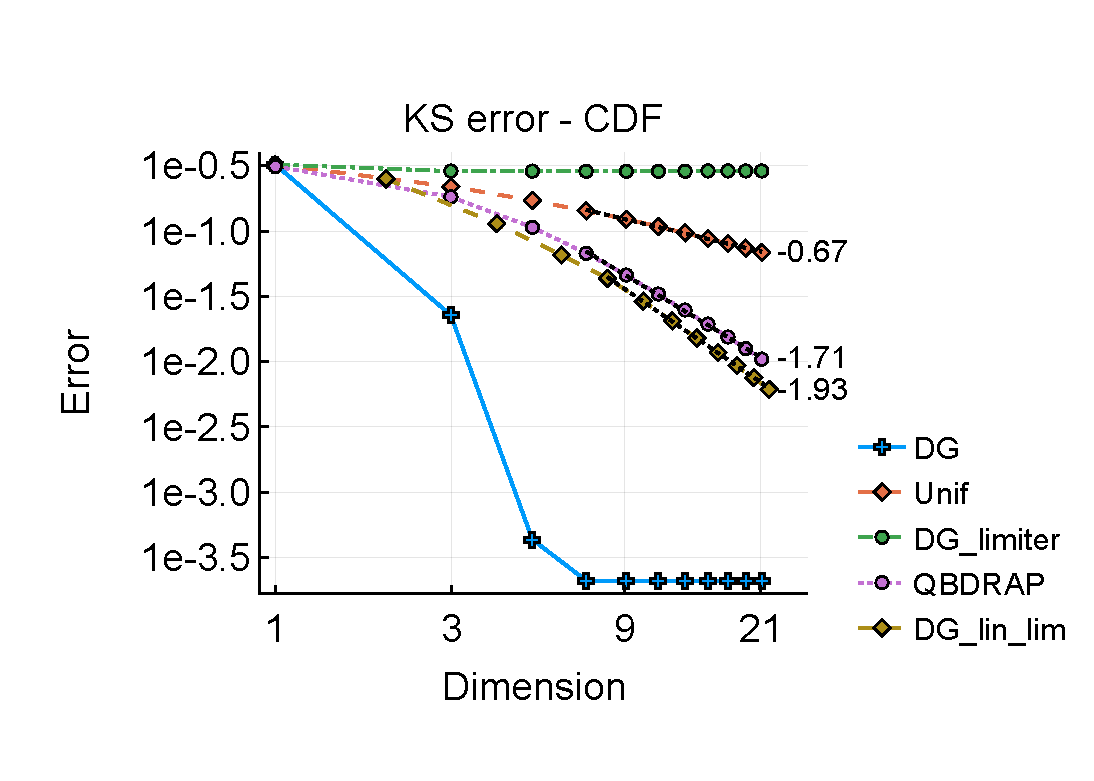
\includegraphics[width=0.5\textwidth,trim={0.75cm 0.8cm 0.25cm 1.25cm},clip]{chapter6/figs/wave/fun6/meshs_ks_error_formatted.pdf}%
		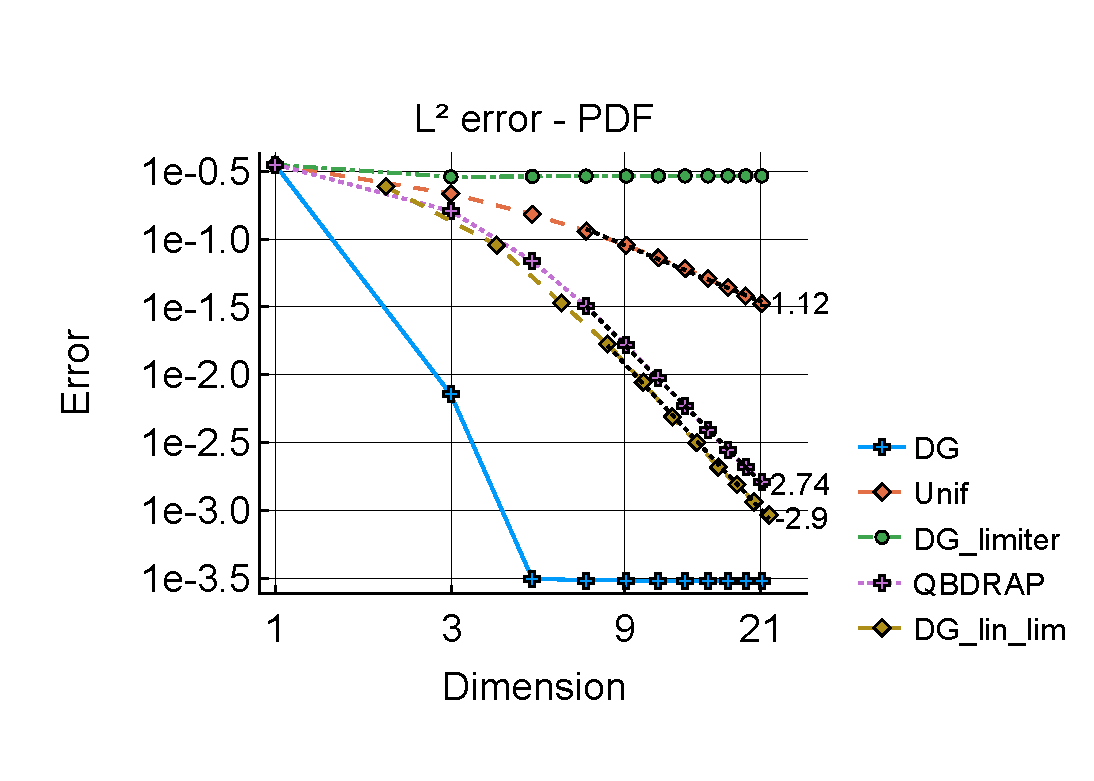
\includegraphics[width=0.5\textwidth,trim={0.75cm 0.8cm 0.25cm 1.25cm},clip]{chapter6/figs/wave/fun6/meshs_l2_pdf_error_formatted.pdf}
		\caption{KS error between the true CDF (Equation (\ref{eqn: bbbbbaabbaa})) and the approximations (left) and \(L^2\) error between the true PDF and the approximations for the DG method (blue solid line with crosses), DG method with the MUSCL limiter (green dash-dotted line with crosses), uniformisation method (orange dashed line with diamonds) and QBD-RAP method (green dash-dotted line with circles).} 
		\label{fig: fun 6 wave} 
	\end{figure}
\end{example}

\begin{example}
	We now want to look at how the methods might handle a point mass. We introduce an ephemeral second phase into the model with phase transition rate \(T_{22}=-1\), and fluid rate \(c_2=0\). The generator is therefore 
	\[T=\left[\begin{array}{cc} 0 & 0 \\ 1 & -1 \end{array}\right].\]

	We suppose that the initial condition is a point mass at the boundary in phase \(2\), i.e.~
	\[\mathbb P(X(0)\leq x, \varphi(0)=2)=1(0\leq x).\] 
	With this inital condition, the transient distribution at time \(t=4\) is 
	\begin{align}
		&\mathbb P(X(4)\leq x,\varphi(4)=1 \mid X(0)=0,\varphi(0)=2) \nonumber 
		\\&= e^{T_{22}4}\left(e^{-T_{22}x}-1\right)1(4< x) + (1-e^{T_{22}4})1(4\leq x) \nonumber
		\\&= e^{-4}\left(e^{4x}-1\right)1(4< x) + (1-e^{-4})1(4\leq x) \label{eqn: asjda}
	\end{align}
	and 
	\begin{align}
		\mathbb P(X(4)\leq x,\varphi(4)=2 \mid X(0)=0,\varphi(0)=2) = e^{-4}1(0\leq x).
	\end{align}
	The PDF at \(t=4\) is discontinuous at \(x=4\). For this problem, all methods can represent the initial condition exactly. 

	Figure~\ref{fig: fun 1 wave} plots the KS error metric between the true and approximated CDFs (right) and the \(L^2\) error metrics between the true and approximated PDFs. Observing Figure~\ref{fig: fun 1 wave}, as expected, since the solution is discontinuous, the DG method with MUSCL limiter does perform well. The uniformisation and QBD-RAP methods appear to converge, with the QBD-RAP method converging faster. DG method converges fastest, however, produces approximations with negative and oscillatory solutions as we might expect given the discontinuity. A selection of approximations to the transient PDF are shown in Figure~\ref{fig: pdf wave fun 1}
	\begin{figure}
		\centering
		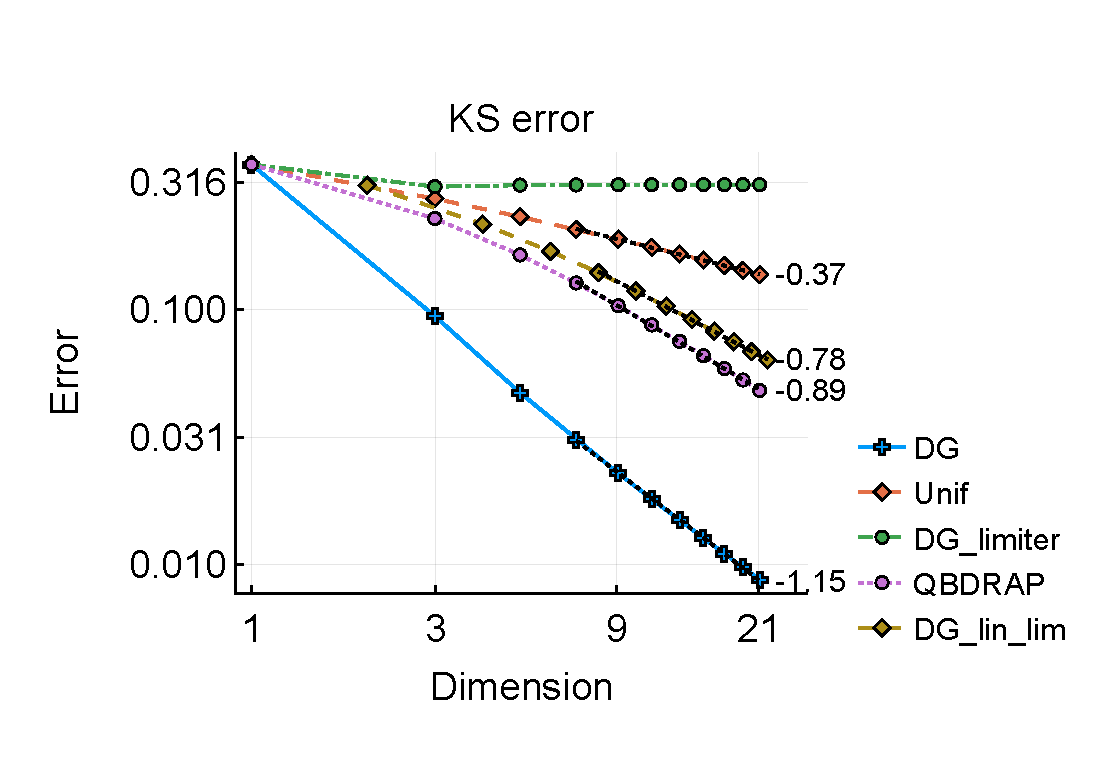
\includegraphics[width=0.5\textwidth,trim={0.75cm 0.8cm 0.25cm 1.25cm},clip]{chapter6/figs/wave/fun1/meshs_ks_error_formatted.pdf}%
		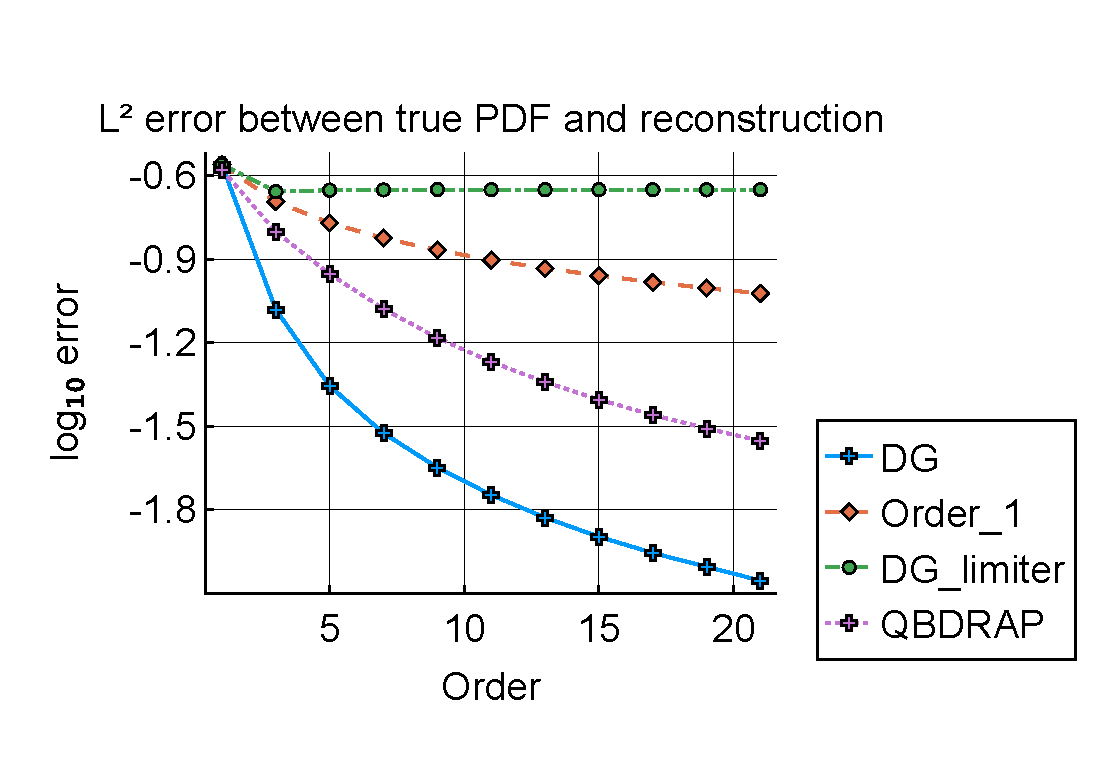
\includegraphics[width=0.5\textwidth,trim={0.75cm 0.8cm 0.25cm 1.25cm},clip]{chapter6/figs/wave/fun1/meshs_l2_pdf_error_formatted.pdf}
		\caption{KS error between the true CDF (Equation (\ref{eqn: asjda})) and the approximations (left) and \(L^2\) error between the true PDF and the approximations for the DG method (blue solid line with crosses), DG method with the MUSCL limiter (green dash-dotted line with crosses), uniformisation method (orange dashed line with diamonds) and QBD-RAP method (green dash-dotted line with circles).} 
		\label{fig: fun 1 wave} 
	\end{figure}
	\begin{figure}
		\centering
		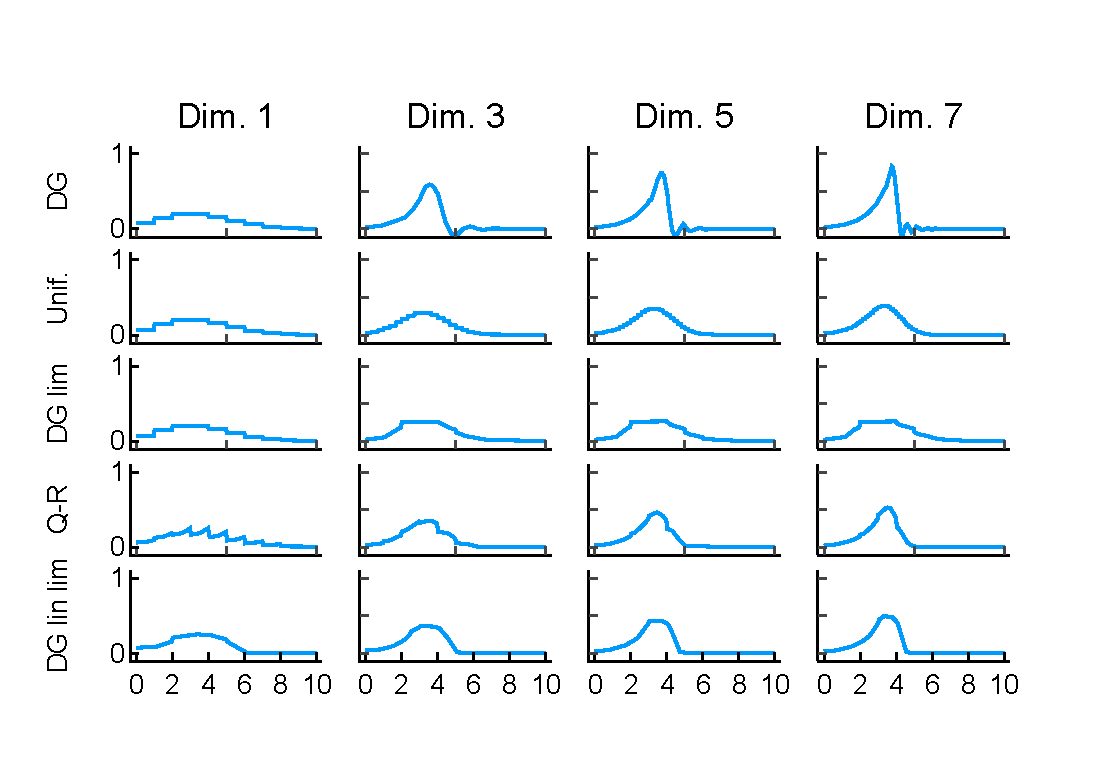
\includegraphics[width=\textwidth]{chapter6/figs/wave/fun1/pdf_formatted.pdf}
		\caption{Reconstructed PDFs using the DG (top row), uniformisation (second row), DG with MUSCL limiter (third row) and QBD-RAP (bottom row) methods, for order 1, 3, 5, and 7 (columns). The true density function is \(e^{-4}e^{x}1(x<4)\).} 
		\label{fig: pdf wave fun 1}
	\end{figure} 
\end{example} 

\FloatBarrier

\section{Stationary distributions} \label{sec:stat}
We briefly turn our attention to stationary distributions of fluid queue. Since the stationary distribution is smooth, apart from at the boundaries, we expect that the DG method will work well here. The stationary distributions are conveninent as they can be evaluated analytically (CITE) and do not require us to approximate initial conditions or integrate over time.

Here we analyse two simple models which are based on Example~2 in \citep{bean2009}, except here we introduce add a lower boundary to the model (no lower boundary is specified in Example~2 of \citep{bean2009} as it is inconsequential to their analysis). 

\begin{model}\label{model: simple}
	Consider a fluid queue where the driving process is a CTMC with state space \(\calS=\{1,2,3,4\}\), generator 
	\[\bs T = \left[\begin{array}{cccc}
		-1.1 & 1.1 & 0 & 0 \\
		1 & -1 & 0 & 0 \\ 
		0.01 & 0 & -0.01 & 0 \\
		0 & 0.01 & 0 & -0.01 
	\end{array}\right],\]
	and there are associated rates \(c_1=1, c_2 = -1, c_3=0, c_4=0\) and boundaries at \(x=0\) and \(x=10\). We specify two types of behaviour at the boundary.
	\begin{enumerate}[a)]
		\item (Absorbing model) Upon hitting the lower boundary, the process transitions from phase \(2\) to phase \(j\) with probability \(p_{2j}\) where 
		\[\vligne{p_{21} & p_{22} & p_{23} & p_{24}} = \vligne{0 & 0 & 1 & 0}.\]
		Upon hitting the upper boundary, the process transitions from phase \(1\) to phase \(j\) with probability \(p_{1j}\) where 
		\[\vligne{p_{11} & p_{12} & p_{13} & p_{14}} = \vligne{0 & 0 & 0 & 1}.\]
		\item (Reflecting model) Upon hitting the lower boundary, the process transitions from phase \(2\) to phase \(j\) with probability \(p_{2j}\) where 
		\[\vligne{p_{21} & p_{22} & p_{23} & p_{24}} = \vligne{1 & 0 & 0 & 0}.\]
		Upon hitting the upper boundary, the process transitions from phase \(1\) to phase \(j\) with probability \(p_{1j}\) where 
		\[\vligne{p_{11} & p_{12} & p_{13} & p_{14}} = \vligne{0 & 1 & 0 & 0}.\]
	\end{enumerate}
\end{model}
Phases~3 and 4 are included only to capture behaviour at the boundary.

For Model~\ref{model: simple}~a), upon hitting the boundary, the process stays at the boundary for an exponentially distributed amount of time with mean 100. For Model~\ref{model: simple}~b), upon hitting the boundary, the process is immediately reflected. In Model~\ref{model: simple}~b) phases 3 and 4 are ephemeral and are included only for notational convenience. 

The models were discretised using the DG, uniformisation and QBD-RAP methods using ten cells of width \(1\). We compute the coefficients for the stationary distribution in the following way. Suppose that a given discretisation method results in an approximation to the generator of the fluid queue as a matrix \(\bs B\). Then the stationary coefficients are found by solving 
\begin{align}
	\bs b \bs B = 0,\\
	\mbox{such that } \bs b\bs 1=1,
\end{align}
for the coefficients \(\bs b\). 

\paragraph{Model~\ref{model: simple}~a) Absorbing model}
Figure~\ref{fig: absorbing stationary} plots KS errors between the true stationary CDF and the approximations (left) and the \(L^2\) error between the true stationary PDF and the approximations. Clearly the DG method is superior here as its error rapidly decrease to a point where is become insignificant compared to other numerical errors. The QBD-RAP method and uniformisation method both appear to be converging, with the errors for the QBD-RAP method decreasing faster.
\begin{figure}
	\centering
	\includegraphics[width=0.5\textwidth,trim={0.75cm 0.8cm 0.25cm 1.25cm},clip]{chapter6/figs/hitting_times_model/absorbing_model/stationary_distribution/ks_error_formatted.pdf}%
	\includegraphics[width=0.5\textwidth,trim={0.75cm 0.8cm 0.25cm 1.25cm},clip]{chapter6/figs/hitting_times_model/absorbing_model/stationary_distribution/l2_pdf_error_formatted.pdf}
	\caption{KS error between the true stationary CDF  and the approximations (left) and \(L^2\) error between the true stationary PDF and the approximations for Model~\ref{model: simple}~a) using the DG method (blue solid line with crosses), uniformisation method (orange dashed line with diamonds) and QBD-RAP method (green dash-dotted line with circles).} 
	\label{fig: absorbing stationary} 
\end{figure}

\paragraph{Model~\ref{model: simple}~b) Reflecting model}
Figure~\ref{fig: reflecting stationary} plots KS errors between the true stationary CDF and the approximations (left) and the \(L^2\) error between the true stationary PDF and the approximations. Once again, the DG method is superior, the QBD-RAP method and uniformisation method both appear to be converging, with the errors for the QBD-RAP method decreasing faster.
\begin{figure}
	\centering
	\includegraphics[width=0.5\textwidth,trim={0.75cm 0.8cm 0.25cm 1.25cm},clip]{chapter6/figs/hitting_times_model/reflecting_model/stationary_distribution/ks_error_formatted.pdf}%
	\includegraphics[width=0.5\textwidth,trim={0.75cm 0.8cm 0.25cm 1.25cm},clip]{chapter6/figs/hitting_times_model/reflecting_model/stationary_distribution/l2_pdf_error_formatted.pdf}
	\caption{KS error between the true stationary CDF and the approximations (left) and \(L^2\) error between the true stationary PDF and the approximations for Model~\ref{model: simple}~b) using the DG method (blue solid line with crosses), uniformisation method (orange dashed line with diamonds) and QBD-RAP method (green dash-dotted line with circles).} 
	\label{fig: reflecting stationary} 
\end{figure}

\section{Transient distributions}
Once again we consider Model~\ref{model: simple}~b)\footnote{We do not include the results for Model~\ref{model: simple}~a) as, for the purposes of the comparisons here, they are much the same as those reported for Model~\ref{model: simple}~b)} and use the same spatial discretisation as described in Section~\ref{sec:stat} (ten cells with width \(\Delta=1\)). Two initial conditions are considered, a point mass at 0.0 in phase 1, and the initial distribution with PDF 
\begin{align}
	\cfrac{1}{2}e^{-x}/(1-e^{-10})\label{eqn: exp init cond}
\end{align}
in phases 1 and 2, with no mass at the boundaries. We numerically integrate over time until time \(t=2.0\) using the SSPRK4 method with t-step size 0.005. We apply the DG method with, and without, the Generalised MUSCL slope limiter. 

To obtain a \emph{ground truth} 5,000,000 realisations of the fluid queue were simulated until \(t=2\), then the empirical CDF and the mass within each cell and at the boundaries were computed from the simulations. We do not attempt to numerically approximate the true PDF via simulation. We then compute the KS and \(L^1\) error metrics between the approximated CDF and simulated CDF, as well as the cell-wise error metric, given as follows. 
\begin{align}
	&\sum_{j\in\{1,2\}}\sum_{\ell=1}^{10} \left|\mathbb P(X(2)\in\calD_{\ell,j}, \varphi(2)=j\mid X(0)=0.5,\varphi(0)=1)-p(2,\ell,j)\right|\nonumber 
	\\&+\left|\mathbb P(X(2)\in\{10\}, \varphi(2)=4\mid X(0),\varphi(0))-p(2,11,4)\right|\nonumber 
	\\&+\left|\mathbb P(X(2)\in\{0\}, \varphi(2)=3\mid X(0),\varphi(0))-p(2,0,3)\right| \label{eqn: cell errors 2}
\end{align}
where \(p(2,\ell,j)\) is an approximation to \(\mathbb P(X(2)\in\calD_{\ell,j}, \varphi(2)=j\mid X(0),\varphi(0))\), \(p(2,11,4)\) is an approximation to \(\mathbb P(X(2)\in\{10\}, \varphi(2)=4\mid X(0),\varphi(0))\), and \(p(2,0,3)\) is an approximation to \(\mathbb P(X(2)\in\{10\}, \varphi(2)=3\mid X(0),\varphi(0))\). 

To account for possible Monte-Carlo error, we used a bootstrap with 1,000 bootstrap samples. That is, we sample, with replacement, 5,000,000 realisations of the fluid queue from the original 5,000,000 samples, then compute error metrics with the resampled data. We resample 1,000 times. Via the bootstrap, we report the \(5\)th and \(95\)th percentile of the sampling distribution of the errors. 

To evaluate error metrics, we use a grid of 10,001 evenly spaced points for each phase. 

To approximate the point mass initial condition we compute the initial coefficients for each scheme exactly. For the exponential initial condition (\ref{eqn: exp init cond}) we compute the initial coefficients via Gauss-Lobatto quadrature for the DG method, by using the mid-point rule for the uniformisation method, and by using a trapezoidal rule with 2,001 points on each cell for the QBD-RAP method. 

\paragraph{Model~\ref{model: simple}~b) Reflecting model with exponential initial condition}
Figure~\ref{fig: reflecting transient exp} shows the error metrics for the four different spatial discretisation schemes (DG, DG with MUSCL limiter, uniformisation and QBD-RAP). For both error metrics the DG scheme converges rapidly until computational errors become significant. The uniformisation and QBD-RAP schemes converge at a slower rate, with the QBD-RAP scheme converging at a faster rate. The DG scheme with MUSCL limiter does not appear to be converging, which suggests there is at least one iteration during the numerical integration over time at which the numerical solution displays oscillations. However, when the DG approximations for the distribution at time \(t=2\) are plotted, they do not display oscillations. This suggests that the oscillations which might occur with the DG scheme must be transient, and have dissipated by time \(t=2\).%
\begin{figure}
	\centering
	\includegraphics[width=0.5\textwidth,trim={0.75cm 0.8cm 0.25cm 1.25cm},clip]{chapter6/figs/hitting_times_model/reflecting_model/transient_distribution/exp/ks_error_formatted.pdf}%
	\includegraphics[width=0.5\textwidth,trim={0.75cm 0.8cm 0.25cm 1.25cm},clip]{chapter6/figs/hitting_times_model/reflecting_model/transient_distribution/exp/l1_cdf_error_formatted.pdf}
	\caption{KS (left) and \(L^1\) (right) errors between the true transient CDF at time \(t=2\) for Model~\ref{model: simple}~b) with the exponential initial condition, and the corresponding approximations obtained via the DG method (blue solid line), DG method with Generalised MUSCL limiter (green dashed line), uniformisation method (orange dashed line) and QBD-RAP method (purple dotted line).} 
	\label{fig: reflecting transient exp} 
\end{figure}

\paragraph{Model~\ref{model: simple}~b) Reflecting model with a point-mass initial condition}
Figure~\ref{fig: reflecting transient pm} shows the error metrics for the four different spatial discretisation schemes (DG, DG with MUSCL limiter, uniformisation and QBD-RAP). Comparing the error metrics in Figure~\ref{fig: reflecting transient pm} for the point mass initial condition, with the ones in Figure~\ref{fig: reflecting transient exp} for the exponential initial condition, all schemes perform worse for the point mass initial condition. Regarding comparative rates of convergence, we come to similar conclusions as we did for the exponential initial condition. The DG scheme converges fastest, followed by the QBD-RAP scheme, then the uniformisation scheme, while the DG scheme with MUSCL limiter does not appear to converge due to the limiter reducing the scheme to a linear approximation in the spatial variable. %
\begin{figure}
	\centering
	\includegraphics[width=0.5\textwidth,trim={0.75cm 0.8cm 0.25cm 1.25cm},clip]{chapter6/figs/hitting_times_model/reflecting_model/transient_distribution/point_mass/ks_error_formatted.pdf}%
	\includegraphics[width=0.5\textwidth,trim={0.75cm 0.8cm 0.25cm 1.25cm},clip]{chapter6/figs/hitting_times_model/reflecting_model/transient_distribution/point_mass/l1_cdf_error_formatted.pdf}
	\caption{KS (left) and \(L^1\) (right) errors between the true transient CDF at time \(t=2\) for Model~\ref{model: simple}~b) with the point-mass initial condition, and the corresponding approximations obtained via the DG method (blue solid line), DG method with Generalised MUSCL limiter (green dashed line), uniformisation method (orange dashed line) and QBD-RAP method (purple dotted line).} 
	\label{fig: reflecting transient pm} 
\end{figure}
\FloatBarrier

\section{Hitting/Exit times}
\begin{model}\label{model: simple2}
Consider an unbounded fluid queue with two phases, generator 
\[\bs T = \left[\begin{array}{cc}
	-1.1 & 1.1 \\
	1 & -1
\end{array}\right],\]
and associated rates \(c_1=1, c_2=-1\). We approximate the first exit time of the interval \([0,1]\). 
\end{model}
Let \(\theta = \{\inf t>0 \mid X(t)=0, \mbox{ or }X(t)=1\},\) then the distribution of the exit time in phase \(i\in\{1,2\}\) is 
\begin{equation}\label{eqn: hit cdf}\mathbb P(\theta < t, \varphi(t)=i\mid \bs X(0)\sim \mu),\end{equation}
for some initial distribution \(\mu\). We look at two initial conditions; an exponential with equal mass in each phase, 
\[\mathbb P(X(0)\in\wrt x,\varphi(0)=i) = exp(-x)/(1-exp(-1))/2,\]
and a point mass at \(X(0)=0\) in phase \(\varphi(0)=1\). 

To do so, we partition \([0,1]\) into three intervals of width \(1/3\), and use the DG, uniformisation and QBD-RAP methods to discretise the fluid queue. To capture the mass which has left the interval \([0,1]\), we suppose that when the process hits the boundary it is absorbed forever at the boundary and remains in the phase which it hit the boundary. 

We integrate the discretisations until time \(t=10\) using the SSPRK4 method with t-step size 0.005. We use the DG scheme with and without a slope limiter during the time-integration. At each time-step of the numerical integration, we record the amount of mass at the absorbing boundaries in each phase, which gives us an approximation of the cumulative distribution function of the exit time in each phase up to time \(t=10\). 

For comparison, we simulated 5,000,000 realisations and recorded the exit time from the interval \([0,1]\) and the phase at the time of exit. We then compute the empirical CDF of the hitting probabilities 
\[\mathbb P(\theta < t, \varphi(t)=i\mid \bs X(0)\sim \mu),\] 
for \(t=0.005\times k\), \(k=0,...,2000\). 

To account for Monte-Carlo errors, we took 1,000 bootstrap resamples of the original 5,000,000 samples and computed the empirical CDF of the hitting probabilities for each bootstrap sample. For each bootstrap sample, we resampled 5,000,000 points. For each bootstrap sample we compute error metrics between the empirical and approximated CDFs and recorded the 5th and 95th percentile of the distribution of the errors. 

\paragraph{Exponential initial condition}
Figure~\ref{fig: hitting time exp} shows the error metrics recorded for the four different numerical approximation schemes. The uniformisation and QBD-RAP method both appear to converge, with the QBD-RAP converging at a faster rate. For both error metrics, the DG scheme converges rapidly to order 5, after which there is no further improvement. The DG scheme with MUSCL limiter does not appear to converge, suggesting oscillations in the DG approximation. However, there are no obvious signs of this oscillation in the exit-time CDF. For the KS-metric, the QBD-RAP scheme outperforms the DG scheme at orders 15, 17 and 21, which, to me, is unexpected. Perhaps the oscillations in the DG scheme are preventing more accurate solutions, or it could be that certain numerical errors in the QBD-RAP scheme have had a favourable cancellation and caused a lower error.
\begin{figure}
	\centering
	\includegraphics[width=0.5\textwidth,trim={0.75cm 0.8cm 0.25cm 1.25cm},clip]{chapter6/figs/hitting_times_model/hitting_times/exp/ks_error_formatted.pdf}%
	\includegraphics[width=0.5\textwidth,trim={0.75cm 0.8cm 0.25cm 1.25cm},clip]{chapter6/figs/hitting_times_model/hitting_times/exp/l1_cdf_error_formatted.pdf}
	\caption{KS (left) and \(L^1\) (right) errors between the simulated and approximated first exit time CDFs (Equation~\ref{eqn: hit cdf}) for Model~\ref{model: simple2} with the exponential initial condition. The approximations were obtained via the DG method (blue solid line), DG method with Generalised MUSCL limiter (orange dashed line), uniformisation method (green dashed line) and QBD-RAP method (purple dotted line). Bootstrapped 90\% confidence intervals are shown by the lighter coloured bars surrounding the lines.} 
	\label{fig: hitting time exp} 
\end{figure}

\paragraph{Point mass initial condition}
Figure~\ref{fig: hitting time pm} shows the error metrics recorded for the four different numerical approximation schemes. The uniformisation and QBD-RAP method both appear to converge, with the QBD-RAP converging at a faster rate. The DG scheme with MUSCL limiter does not appear to converge, suggesting oscillations in the DG approximation. The DG scheme appears to converge fastest up to the order-19 scheme, at which point the error increases. This is caused by oscillations in the numerical solution. In this case we can observe the oscillation in the exit time CDF. 

In Figure~\ref{fig: hitting time oscillation} we plot the CDFs of the exit time for phase 1, obtained via the DG scheme and QBD-RAP scheme, each using an order-21 basis, and also via simulation. Observing Figure~\ref{fig: hitting time oscillation} the DG approximation clearly displays oscillations around \(t=0\) and \(t=1\). The largest oscillations are around \(t=0\). 
\begin{figure}
	\centering
	\includegraphics[width=0.5\textwidth,trim={0.75cm 0.8cm 0.25cm 1.25cm},clip]{chapter6/figs/hitting_times_model/hitting_times/point_mass/ks_error_formatted.pdf}%
	\includegraphics[width=0.5\textwidth,trim={0.75cm 0.8cm 0.25cm 1.25cm},clip]{chapter6/figs/hitting_times_model/hitting_times/point_mass/l1_cdf_error_formatted.pdf}
	\caption{KS (left) and \(L^1\) (right) errors between the simulated and approximated first exit time CDFs (Equation~\ref{eqn: hit cdf}) for Model~\ref{model: simple2} with the point mass initial condition. The approximations were obtained via the DG method (blue solid line), DG method with Generalised MUSCL limiter (orange dashed line), uniformisation method (green dashed line) and QBD-RAP method (purple dotted line). Bootstrapped 90\% confidence intervals are shown by the lighter coloured bars surrounding the lines.} 
	\label{fig: hitting time pm} 
\end{figure}
\begin{figure}
	\centering
	\includegraphics[width=\textwidth]{chapter6/figs/hitting_times_model/hitting_times/point_mass/cdf_order21DG_and_sims.pdf}%
	\caption{Approximations of the CDF of the first exit time in phase 1 for Model~\ref{model: simple2} with the point mass initial condition. The blue line was obtained from the order-21 DG scheme, the purple dotted line from the order-21 QBD-RAP scheme, and the gold dashed line is the empirical CDF obtained via simulation. The DG scheme displays oscillations. } 
	\label{fig: hitting time oscillation} 
\end{figure}

\section{First-return times of fluid-fluid queues}
Here we approximate a model considered in \cite{blnos2022} which is a modified version of a model first presented in \cite{lnp13}. 
\begin{model}\label{model: ffq}
	Consider a stochastic fluid-fluid queue $\{(X(t),Y(t),\varphi(t))\}_{t\geq0},$ where $\{X(t)\}$ and $\{Y(t)\}$ represent the workloads in Buffers~1 and~2 at time $t \geq 0$, respectively, both driven by the phase $\{\varphi(t)\},$ which is a Markov chain on the state space $\mathcal{S} = \{11,10,01,00\}$. Both $\{X(t)\}$ and $\{Y(t)\}$ have a regulated boundary at 0. Here, the state $11$ indicates inputs to both buffers being \textsc{on}, the state $00$ indicates both being \textsc{off}, the state $10$ is when only the first input is \textsc{on}, and the state $01$ is when only the second is \textsc{on}. The input of Buffer~$k$ is switched from \textsc{on} to \textsc{off} with rate $\gamma_k$, and from \textsc{off} to \textsc{on} with rate $\beta_k$, for $k = 1, 2$. Thus, the infinitesimal generator $T$ for $\varphi(t)$ is given by 
	\begin{align*} 
		T = \left[ \begin{array}{cccc} -(\gamma_1 + \gamma_2) & \gamma_2 & \gamma_1 & 0 \\
							\beta_2 & -(\gamma_1 + \beta_2) & 0 & \gamma_1 \\
							\beta_1 & 0 & -(\gamma_2 + \beta_1) & \gamma_2 \\
							0 & \beta_1 &\beta_2 &-(\beta_1 + \beta_2)
	\end{array}\right].
	\end{align*} 

	The net rates of change for $X(t)$, denoted $c_i$, are given by 
	% 
	\begin{align*} 
	& (c_{11},c_{10},c_{01},c_{00})   =  \begin{array}{rrrr} 
	(\lambda_1-\theta_1,  & \lambda_1 -\theta_1, &  -\theta_1, & -\theta_1),
	\end{array}  
	\end{align*} 
	% 
	and the net rates of change for $Y(t)$, denoted $r_i$, are as follows  
	%  
	\begin{align*} 
	(r_{11},r_{10},r_{01},r_{00})  & = \left\{ \begin{array}{lrrrll}  
	% (\lambda_2 -\kappa, & \;\;\;\;0, & \lambda_2 - \kappa, &  \;\;\;\;0) & \text{if } X_t = 0,  Y_t = 0,\\
	%  \vspace*{-0.3cm} \\
												(\lambda_2 - \kappa, & \;\;\;-\kappa,  & \lambda_2 - \kappa, & -\kappa) &\text{if } X_t = 0, \\
												\vspace*{-0.3cm} \\
	%	(\lambda_2 -\theta_2,  &  0,  & \lambda_2 - \theta_2,  & \;\;\;\; 0) & \text{if } X_t \in (0,x^*), Y_t = 0,\\
	%											  \vspace*{-0.3cm} \\
		(\lambda_2 - \theta_2, & -\theta_2, & \lambda_2 - \theta_2, & -\theta_2) & \text{if } X_t \in (0,x^*),\\
												\vspace*{-0.3cm} \\
		(\;\;\;\;\;\;\; \lambda_2, & \;\;\;\;0, & \lambda_2, &  \;\;\;\;0) & \text{if } X_t \geq x^*. \end{array}
												\right.
	\end{align*} 

	For our numerical experiments, we use the parameter choices given in~\citep{lnp13}: 
	% 
		\begin{align} 
			\label{eqn:parameters}
		\gamma_1 & =11, \quad  \beta_1 = 1, \quad \lambda_1 = 12.48, \quad  \theta_1 = 1.6, \quad  \kappa = 2.6, \\
			\label{eqn:parameters-2}
		\gamma_2 & = 22, \quad \beta_2  = 1, \quad  \lambda_2 = 16.25, \quad \theta_2 = 1.0, \quad x^* = 1.6.
		\end{align} 
\end{model}
	
While the true problem has an unbounded domain $[0,\infty)$, the approximations require the domain of approximation to be a finite interval. Here we choose an upper bound of \(48\) and place a regulated boundary at the upper boundary. The effect of this truncation can be partly quantified by evaluating \(\lim\limits_{t\to\infty}\mathbb P\left(X(t) > 48\right)\approx 5.83 \times 10^{-9}\), \(i\in\calS\). 

We obtained approximations to the infinitesimal generator of the fluid queue \(\{(X(t),\varphi(t))\}_{t\geq 0}\) via the DG method, QBD-RAP method and uniformisation method, all of which used a cell width of \(\Delta=0.4\). The matrix resulting from the approximation is then used to approximate the first-return operator \(\Psi(s)\) as discussed in Section~\ref{SOME INTRO SECTION}. Due to the stochastic interpretation of the uniformisation and QBD-RAP schemes, the approximations to \(\Psi(s)\) have a stochastic interpretation as the first-return probabilities of a fluid queue driven by a CTMC and QBD-RAP, respectively. For the DG method the approximation of \(\Psi(s)\) is not well-understood. However, I believe that the resulting operator is a projection operator which, given an initial distribution, projects the distribution of \(X(\theta_2)\) on to a set of polynomial basis functions, much like the DG method itself. 

Ultimately, we want to approximate the first-return distribution 
\begin{align}\label{eqn: first return Y 1}
	\mathbb P(X(\theta_2)\leq x, \varphi(\theta_2)=i\mid \bs X(0)\sim \mu).
\end{align}
For Model~\ref{model: ffq}, it is only possible for the process \(Y(t)\) to return to \(0\) at time \(t\) when \((X(t),\varphi(t))\in[0,1.6)\times \{10,00\}\). As such, evaluate the approximations over this region only. We use a grid of 10,001 points at which to evaluate the approximations of the CDF in each phase. We consider first the initial distribution which is a point mass at \(Y(0)=0,\, X(0)=5,\, \varphi(0)=01\). 

For comparison, we simulated 5,000,000 realisations of the fluid-fluid queue and recorded the value of \(X\) and \(\varphi\) at the time of first return of the second fluid, \(Y\). The empirical approximation of (\ref{eqn: first return Y 1}) was then constructed, and error metrics for the difference between the empirical CDF and the approximations was computed. To account for Monte-Carlo errors, we used a bootstrap with 1,000 bootstrap samples to construct 1,000 bootstrap samples of the error estimates and recorded the 5th and 95th percentiles of the error distribution. Each of the 1,000 bootstrap samples was constructed by resampling the original 5,000,000 realisations 5,000,000 times, with replacement.

In Figure~\ref{fig: ffq return cts} we plot the error metrics for the approximations to the distribution (\ref{eqn: first return Y 1}). The DG method performs best converging rapidly until the error in the approximation scheme is swamped by other numerical errors. Here, the first return distribution appears to be smooth, hence we might expect the DG method to perform well. Note that there is a significant number other sources of error here; machine precision errors, errors in solving the Ricatti equation to approximate \(\Psi(s)\), errors from approximating error metrics (numerical integration/finding KS statistic), and truncation errors. Furthermore, for the QBD-RAP, since the parameters \(\bs \alpha,\,\bs S,\,\bs s\,\) and \(\bs D\) are found numerically, then there is another source of error from this. 

Figure~\ref{fig: ffq return cts} also shows that the uniformisation and QBD-RAP methods also appear to be converging, albeit, at a slower rate. 
\begin{figure}
	\centering
	\includegraphics[width=0.5\textwidth,trim={0.75cm 0.8cm 0.25cm 1.25cm},clip]{chapter6/figs/ffq/cts/ks_error_formatted.pdf}%
	\includegraphics[width=0.5\textwidth,trim={0.75cm 0.8cm 0.25cm 1.25cm},clip]{chapter6/figs/ffq/cts/l1_cdf_error_formatted.pdf}
	\caption{KS (left) and \(L^1\) (right) errors between the simulated and approximated CDFs of \(X(\theta_2)\) (Equation~\ref{eqn: first return Y 1}) for Model~\ref{model: ffq}. The approximations were obtained via the DG method (blue solid line), uniformisation method (green dashed line) and QBD-RAP method (purple dotted line). Bootstrapped 90\% confidence intervals are shown by the lighter coloured bars surrounding the lines.} 
	\label{fig: ffq return cts} 
\end{figure}

By modifying slightly Model~\ref{model: ffq}, we can construct a first return distribution which is discontinuous. 
\begin{model}\label{model: ffq2}
	Consider a fluid-fluid queue which is the same as Model~\ref{model: ffq} except 
	\begin{align}
		r_{00}(X(t)) = \begin{cases}
			-\kappa, & \mbox{ if }X(t)=0,\\
			-\theta_2, & \mbox{ if }X(t)=\in(0,x^*),\\
			\theta_2, & \mbox{ if }X(t)\geq x^*.
		\end{cases}
	\end{align}
	Further, consider the initial distribution which is a point-mass at \(Y(0)=0,\, X(0)=2, \varphi(0)=00\).
\end{model}
As before, we use the DG, uniformisation and QBD-RAP methods to approximate the model, and compare to simulations. 

For Model~\ref{model: ffq2} there is a point mass at \(X(\theta_2)=1.2\) of magnitude \(e^{-(\beta_1+\beta_2)}\times 0.5\), which occurs when the phase remains \(\varphi(t)=00\) until this \(\theta_2\).

Figure~\ref{fig: ffq return discts} plots the error metrics for the first return distribution. Observing Figure~\ref{fig: ffq return discts} we see that the DG method performs well, followed by the QBD-RAP method, then the uniformisation method performs worst. However, the DG method results in an oscillatory solution with the CDF taking impossible values (decreasing at points) as shown in Figure~\ref{fig: ffq2 oscillation}
\begin{figure}
	\centering
	\includegraphics[width=0.5\textwidth,trim={0.75cm 0.8cm 0.25cm 1.25cm},clip]{chapter6/figs/ffq/discts/ks_error_formatted.pdf}%
	\includegraphics[width=0.5\textwidth,trim={0.75cm 0.8cm 0.25cm 1.25cm},clip]{chapter6/figs/ffq/discts/l1_cdf_error_formatted.pdf}
	\caption{KS (left) and \(L^1\) (right) errors between the simulated and approximated CDFs of \(X(\theta_2)\) (Equation~\ref{eqn: first return Y 1}) for Model~\ref{model: ffq2}. The approximations were obtained via the DG method (blue solid line), uniformisation method (green dashed line) and QBD-RAP method (purple dotted line). Bootstrapped 90\% confidence intervals are shown by the lighter coloured bars surrounding the lines.} 
	\label{fig: ffq return discts} 
\end{figure}
\begin{figure}
	\centering
	\includegraphics[width=\textwidth]{chapter6/figs/ffq/discts/phase_4_cdf.pdf}%
	\caption{Approximations of the CDF of the first exit time in phase 1 for Model~\ref{model: simple2} with the point mass initial condition. The blue line was obtained from the order-21 DG scheme, the purple dotted line from the order-21 QBD-RAP scheme, and the gold dashed line is the empirical CDF obtained via simulation. The DG scheme displays oscillations. } 
	\label{fig: ffq2 oscillation} 
\end{figure}

\FloatBarrier
\section{Discussion}
In this chapter we have numerically investigated some properties of the QBD-RAP approximation scheme and compared it to existing methods; the uniformisation scheme of \cite{bo2013} and the discontinuous Galerkin scheme. In general, the numerical experiments show that, for problems with discontinuities, the DG approximation can exhibit oscillations and negativity, while the QBD-RAP and uniformisation approximations avoid this and, of the latter two, the QBD-RAP scheme often converges faster. To avoid the problems of oscillations and negativity, we can sometimes employ a \emph{slope limiter} with the DG scheme, which effectively reduces the scheme to linear in the regions where oscillations are detected. The numerical experiments demonstrate the loss of accuracy in the approximation when a slope limiter is used for a discontinuous problem. Moreover, for the application of the methods to fluid-fluid queues, there is no useful way to apply the concept of a slope limiter. %When the slope limiter detects oscillations in the approximate solution, it reduces the DG scheme to linear in the region surrounding the oscillations, otherwise, the slope limiter leaves the solution unchanged. Thus, the slope limiter permits high-order approximations away from oscillations, while also removing oscillations. 
In general, we observe that the smoother the problem the better the performance of the DG method, and it rapidly surpasses the performance of the other two methods. For smooth problems the DG method is almost unbeatable. 

As a first step in the numerical experiments, we examined the ability for each method to approximate different initial conditions. For the DG method, this is equivalent to a projection of the initial condition on to a set of basis polynomials. For the uniformisation method this is equivalent to projecting the initial condition on to a basis of constant functions. Section~\ref{sec: comp} demonstrates that the DG (projection) scheme can result in oscillations and negative regions in the approximation when the initial condition is discontinuous. The uniformisation and QBD-RAP methods avoid this problem, but appear to have higher errors and the QBD-RAP method appears to have the largest errors. For discontinuous initial conditions the rates of convergence are comparable for all three methods. However, when the initial condition to be approximated is sufficiently smooth, then the DG approximation is \emph{far} superior. 

Next, we instrumented the performance of approximations for a simple travelling wave problem with various initial conditions. For this problem the solution is given in terms of the initial condition by \(f(x,t) = f(x-t,0)\). Once again, for discontinuous problems, the DG method can display oscillations and negativity, while the other methods (DG with slope limiter, uniformisation and QBD-RAP methods) avoid this. Further, for discontinuous problems the rates of convergence of the QBD-RAP and DG methods can be similar. For smooth problems the DG method is superior. 

We then instrument the performance of the approximations on a simple fluid queue. We first look at the stationary distribution, which is known to be smooth. Since the problem is smooth, then the DG method is superior as expected. Of the uniformisation and QBD-RAP methods, the QBD-RAP method gives more accurate solutions. We then turn our attention to approximating transient distributions for the same models and consider two different initial conditions, a point-mass and an exponential initial condition. The discontinuous initial condition results in a discontinuous transient distribution. As for the exponential initial condition, this example demonstrates that, even if the initial condition appears `nice', it can still result in discontinuous, or non-differetiable solutions. The numerical evidence suggests that the DG method can display oscillations, while the other methods do not. The DG method with slope limiter detects the oscillations and reduces the method to linear. Of the uniformisation and QBD-RAP methods, the latter performs better. 

Next we look at exit times for the same fluid queue with two initial conditions, an exponential initial condition and a point-mass. We look at the exit time of the fluid level from the interval \((0,1)\). For this problem there is never any in-flow of mass at the boundaries of the interval and so, for a solution to be continuous, the initial condition needs to be chosen carefully, otherwise discontinuities in the \textit{transient distribution} may result, as is the case for both initial conditions here. The numerical results suggest that, due to the discontinuities in the problems, the DG method can perform not as well as we might expect. Since the uniformisation and QBD-RAP methods can handle discontinuities, they perform as expected, with the QBD-RAP method performing better than the uniformisation. 

Lastly, we apply the DG, uniformisation and QBD-RAP methods to some simple fluid-fluid queues. In the first example, which appears to have a smooth solution, the DG method performs very well. Of the other two methods the QBD-RAP method performs better than the uniformisation. In the second example, which has a discontinuity, the DG method produces the lowest errors, but exhibits oscillations in the solution. The other two methods do not produce oscillations, and of the two the QBD-RAP method performs best. 

In conclusion, when the problem is known to be smooth, the DG method is very likely to produce excellent results. However, for discontinuous problems, the method can show oscillations and infeasible or negative regions of the solution. The slope limiter overcomes this, but reduces the accuracy of the DG method to linear near discontinuities, sometimes severely affecting the quality of the approximation. The uniformisation and QBD-RAP methods are alternative approximation schemes which exhibit larger errors, but avoid oscillatory solutions and ensure positivity. Of uniformisation and QBD-RAP methods, the latter seems to produce lower errors. 

%!TEX root = ../thesis.tex
\chapter{Conclusions \label{ch: conclusion}} 
% add as many as you like

\appendix
% Import the appendices 
% %!TEX root = ../thesis.tex
\chapter{Mathematical background}\label{app: math background}
\section{Laplace Transforms}
The Laplace transform is an important tool in many areas of mathematics, and is particularly useful in the analysis of fluid queues and fluid-fluid queues. Furthermore, in Chapters~\ref{sec: conv} and~\ref{ch: global results} we work with {Laplace transforms} to prove convergence of the QBD-RAP scheme. 

For a measure \( \mu\), defined on the Borel sets of \([0,\infty)\), we define the Laplace transform of \(\mu\) to be
\[\widehat \mu(\lambda) = \mathcal L(\mu)(\lambda) = \int_{t=0}^\infty e^{-\lambda t}\wrt \mu,\]
where the \emph{region of convergence} is the set of values of \(\lambda\in\mathbb R\) such that the integral is finite. When \(\mu\) has a density, \(v\), then the Laplace transform is 
\[\widehat \mu(\lambda) = \widehat v(\lambda) = \mathcal L(v)(\lambda) = \int_{t=0}^\infty e^{-\lambda t}v(x)\wrt x.\]
When \(\mu\) is the probability measure associated with a random variable, \(Z\), say, then we may write 
\[\widehat \mu(\lambda)=\mathbb E[e^{-\lambda Z}],\]
and the region of convergence is at least \([0,\infty)\). 
Further, letting \(E^\lambda\) be an exponentially distributed random variable with rate \(\lambda\) and noting that \(\mathbb P(E^\lambda >t ) = e^{-\lambda t}\), then 
\[\widehat \mu(\lambda)=\mathbb P(Z<E^\lambda),\]
which gives a probabilistic interpretation of the Laplace transform. That is, the Laplace transform with parameter \(\lambda >0\) is the probability that \(Z\) occurs before \(E^\lambda\), an independent random exponential time with rate \(\lambda\), occurs. 

A convenient property of the Laplace transform which we utilise is the Convolution Theorem. 
\begin{thm}[Convolution Theorem]
	Let \(f,g: [0,\infty) \to \mathbb R\) be integrable functions, then 
	\[\mathcal L\left(\int_{u=0}^tf(u)g(t-u)\wrt u\right)(\lambda) = \mathcal L\left(f\right)\cdot \mathcal L\left(g\right).\]
\end{thm}
The Convolution Theorem states that the Laplace transform of the convolution, given by \(\displaystyle \int_{u=0}^tf(u)g(t-u)\wrt u\), is equal to the product of the Laplace transform of \(f\) and \(g\). 

The Laplace transform is unique in the sense that, if \(\mu\) and \(\nu\) are two measures on the Borel sets of \([0,\infty)\) and 
\[\widehat \mu(\lambda) = \widehat \nu(\lambda)\] 
for all \(\lambda > a\) with \(a<\infty\), then \(\mu\) and \(\nu\) are the same. In terms of functions, \(f,g: [0,\infty) \to \mathbb R\), if 
\[\mathcal L(f)(\lambda) = \mathcal L(g)(\lambda),\]
for all \(\lambda > a\) with \(a<\infty\), and \(f\) and \(g\) are continuous, then \(f(t)=g(t)\) for all \(t\geq 0\). Without knowing \(f\) and \(g\) are continuous, then we can only claim that 
\(f(t)=g(t)\) for all \(t\geq 0, t\notin \mathcal N,\) where \(\mathcal N\) is a \emph{null set} with respect to Lebesgue measure. 


\section{Kronecker products and related results}\label{sec:ksdfkkakaaaaaa}
Here we describe Kronecker products and sums and some of their properties (see \cite{MEinAP}, and also Appendix A.4, for further details). We use the results in this section to manipulate certain matrix expressions in Chapter~\ref{sec: conv}.

Let 
\[\bs A = \left[\begin{array}{ccc}a_{11} & \dots & a_{1m}\\\hdots & & \hdots \\ a_{n1}&\dots & a_{nm}\end{array}\right]
\qquad
\bs{B} = \left[\begin{array}{ccc}b_{11} & \dots & b_{1m'}\\\hdots & & \hdots \\ b_{n'1}&\dots & b_{n'm'}\end{array}\right]\]
be matrices with dimensions \(n\times m\) and \(n'\times m'\), respectively. The operator \(\otimes\) is the Kronecker product of two matrices; 
\[\bs A\otimes \bs{B} = \left[\begin{array}{ccc}a_{11}\bs{B} & \dots & a_{1m}\bs{B}\\\hdots & & \hdots \\ a_{n1}\bs{B}&\dots & a_{nm}\bs{B}\end{array}\right],\]
which is an \(nn'\times mm'\) matrix. 

Let \(\bs{C},\bs{D}\)  be matrices with dimensions \(m\times k\) and \(m'\times k'\). A property of the Kronecker Product is 
\begin{align}
	\left(\bs A\otimes \bs{B}\right)\left(\bs{C}\otimes \bs{D}\right) &= \bs A\bs{C}\otimes \bs{B}\bs{D}.\label{eqn:mpr}\tag{Mixed Product Rule}
\end{align}

% \begin{proof}
% 	The proof follows from 
% 	\begin{align*}
% 		\left[\begin{array}{cccc}a_{i1}\bs{B} & a_{i2}\bs{B}&\dots&a_{in}\bs{B}\end{array}\right]\left[\begin{array}{c}c_{1j}\bs{D}\\c_{2j} \bs D \\\vdots\\c_{nj}\bs{D} \end{array}\right] 
% 		%
% 		&= \left(\sum_\ell a_{i\ell}c_{\ell j}\right) \bs{B}\bs{D}
% 		\\&= \left(\bs A\bs{C}\right)_{ij}\bs{B}\bs{D}.
% 	\end{align*}
% \end{proof}

If \(\bs A\) and \(\bs{B}\) are invertible matrices, then 
\begin{align}\label{eqn:kron inverse}
	\left(\bs A\otimes \bs{B}\right)^{-1} = \bs A^{-1}\otimes \bs{B}^{-1}.
\end{align}

Let \(\bs A\) and \(\bs{B}\) be \(n\times n\) and \(m\times m\) matrices, respectively. The Kronecker sum of \(\bs A\) and \(\bs{B}\) is denoted by \(\oplus\) and defined as 
\[\bs A\oplus \bs{B} = \bs A\otimes \bs{I}_{m} + \bs{I}_{n}\otimes \bs{B}.\]

The exponential of a square matrix \(\bs B\) is \[e^{\bs B} = \sum_{n=0}^\infty \cfrac{1}{n!}\bs B^n.\]

A property of the Kronecker sum is 
\begin{align}\label{eqn:kron exp}
	e^{\bs A\oplus \bs{B}}= e^{\bs A}\otimes e^{\bs{B}}.
\end{align}
% \begin{proof}
% 	First, the matrices \(\bs A\otimes \bs{I}_m\) and \(\bs{I}_n\otimes \bs{B}\) commute; from the mixed product rule their product is \(\bs A\otimes \bs{B}\). Hence, 
% 	\[e^{\bs A\oplus \bs{B}} = e^{\bs A\otimes \bs{I}_m}e^{\bs{I}_n\otimes \bs{B}}.\]
% 	We now show that \(e^{\bs A\otimes \bs{I}_m} = e^{\bs A}\otimes \bs{I}_m\) and \(e^{\bs{I}_n\otimes \bs{B}}=\bs{I}_n\otimes e^{\bs{B}}\). The latter follows from the fact that \(\bs{I}_n\otimes \bs{B}\) is a block diagonal matrix with blocks \(\bs{B}\), hence its exponential is also block diagonal with blocks equal to the exponential of \(\bs{B}\). The former follows from 
% 	\begin{align}
% 	e^{\bs A\otimes \bs{I}_m} &= \sum_{n=0}^\infty \cfrac{1}{n!}\left(\bs A\otimes \bs{I}_m\right)^n \nonumber
% 	\\&= \sum_{n=0}^\infty \cfrac{1}{n!}\left(\bs A^n\otimes \bs{I}_m\right) \nonumber
% 	\\&=\left(\sum_{n=0}^\infty \cfrac{1}{n!}\bs A^n\otimes \bs{I}_m\right) \nonumber
% 	\\&=e^{\bs A}\otimes \bs{I}_m.\label{eqn:09ksdjgah}
% 	\end{align}
	
% 	Therefore 
% 	\[e^{\bs A\oplus \bs{B}} = \left(e^{\bs A}\otimes \bs{I}_m\right)\left(\bs{I}_n\otimes e^{\bs{B}}\right),\]
% 	and the result follows by the mixed product rule. 
% \end{proof}

\begin{lem}\label{lem: lst mpr}
	Let \(\bs{T}\) and \(\bs{C}\) be \(n\times n\), square matrices with \(\bs{C}\) diagonal and invertible; let \(\bs{S}\) be a \(p\times p\) matrix. Further, suppose \(\left[\bs{T}\otimes \bs{I} + \bs{C}\otimes \bs{S} - \lambda \bs{I}\right]\) is invertible for \(\lambda>0\). Then
\begin{align}
	&\int_{t=0}^\infty e^{-\lambda t}  e^{{\left(\bs{T}\otimes \bs{I} + \bs{C}\otimes \bs{S}\right)t}} \wrt t 
	%
	=   \int_{x=0}^\infty e^{{\bs{C}^{-1}\left(\bs{T}-\lambda \bs{I}\right)x}}\otimes e^{\bs{S}x} \wrt x \left(\bs{C}\otimes \bs{I}\right)^{-1}.  \label{eqn:lstsimplify}\end{align}
\end{lem}
\begin{proof}
	Computing the integral on the left-hand side and then factorising the result and using the~\ref{eqn:mpr} multiple times gives
	\begin{align}
            	\int_{t=0}^\infty e^{-\lambda t} e^{\left(\bs{T}\otimes \bs{I} + \bs{C}\otimes \bs{S}\right)t} \wrt t\nonumber 
            	%
            	&= - \left[\bs{T}\otimes \bs{I} + \bs{C}\otimes \bs{S} - \lambda \bs{I}\right]^{-1}
		%
		\\&= -  \left[\bs{T}\otimes \bs{I} + \left(\bs{C}\otimes \bs{I}\right)\left(\bs{I}\otimes \bs{S}\right) - \lambda \bs{I}\right]^{-1}\nonumber
		%
		\\&= -  \left[\left(\bs{C}\otimes \bs{I}\right)\left(\left(\bs{C}\otimes \bs{I}\right)^{-1}\left(\bs{T}\otimes \bs{I} \right)+ \bs{I}\otimes \bs{S} - \left(\bs{C}\otimes \bs{I}\right)^{-1}\lambda \bs{I}\right)\right]^{-1}. \label{eqn: ref this one 12}
		%
	\end{align}
	By Equation~(\ref{eqn:kron inverse}) and since \(\bs{C}\) is invertible, (\ref{eqn: ref this one 12}) is equal to
	\begin{align}
		& - \left[\left(\bs{C}\otimes \bs{I}\right)\left(\left(\bs{C}^{-1}\otimes \bs{I}\right)\left(\bs{T}\otimes \bs{I} \right)+ \bs{I}\otimes \bs{S} - \left(\bs{C}^{-1}\otimes \bs{I}\right)\lambda \bs{I}\right)\right]^{-1}. \label{eqn: ref this one 13}
		%
	\end{align}
	{Using the~\ref{eqn:mpr} and algebraic manipulation, (\ref{eqn: ref this one 13}) is equal to }
	\begin{align}
		&- \left[\left(\bs{C}\otimes \bs{I}\right)\left(\left(\bs{C}^{-1}\bs{T}\right)\otimes \bs{I} + \bs{I}\otimes \bs{S} - \left(\bs{C}^{-1}\lambda \bs{I}\right)\otimes \bs{I}\right)\right]^{-1} \nonumber
		%
		\\&= - \left[\left(\bs{C}\otimes \bs{I}\right)\left(\left(\bs{C}^{-1}\left(\bs{T}-\lambda \bs{I}\right)\right)\otimes \bs{I} + \bs{I}\otimes \bs{S}\right)\right]^{-1} \nonumber
		%
		\\&= - \left[\left(\bs{C}^{-1}\left(\bs{T}-\lambda \bs{I}\right)\right)\otimes \bs{I} + \bs{I}\otimes \bs{S}\right]^{-1}\left(\bs{C}\otimes \bs{I}\right)^{-1} \nonumber
		\\&= - \left[\left(\bs{C}^{-1}\left(\bs{T}-\lambda \bs{I}\right)\right)\oplus \bs{S}\right]^{-1}\left(\bs{C}\otimes \bs{I}\right)^{-1},\label{eqn: is an integral}
	\end{align}
	by definition of the Kronecker sum.
	
	Now, for an invertible matrix \(\bs A\) we can write \(-\bs A^{-1} = \displaystyle\int_{x=0}^\infty e^{\bs Ax}\wrt x\). Therefore, (\ref{eqn: is an integral}) is 
	\begin{align*}
		-\left[\left(\bs{C}^{-1}\left(\bs{T}-\lambda \bs{I}\right)\right)\oplus \bs{S}\right]^{-1}\left(\bs{C}\otimes \bs{I}\right)^{-1}
		&= \int_{x=0}^\infty e^{\left(\bs{C}^{-1}\left(\bs{T}-\lambda \bs{I}\right)x\right)\oplus \bs{S}x}\wrt x\left(\bs{C}\otimes \bs{I}\right)^{-1}.
	\end{align*}
	{Using the rule in Equation~(\ref{eqn:kron exp}) gives }
	\begin{align*}
		&\int_{x=0}^\infty e^{\left(\bs{C}^{-1}\left(\bs{T}-\lambda \bs{I}\right)\right)x}\otimes e^{ \bs{S}x}\wrt x\left(\bs{C}\otimes \bs{I}\right)^{-1},
	\end{align*}
	which is the result.
\end{proof}

% vector space? Polynomial basis?
% me basis? semigroup? generator? 

%Laplace transforms of probability measures with non-negative support and where the Laplace transform variable, \(\lambda\), is real and non-negative can be given a stochastic interpretation. Let \(W\) be a random variable with distribution function \(F_W(w)= \mathbb P(W<w)\), then \(\displaystyle\int_{w=0}^\infty e^{-\lambda w} \wrt F_W(w) = \mathbb P(W < E^{\lambda})\). That is, the Laplace transform with parameter \(\lambda >0\) is the probability that \(W\) occurs before \(E^\lambda\), an independent random exponential time with rate \(\lambda\), occurs. 

\section{Convergence theorems}
We use the following convergence theorems to help us prove that the QBD-RAP scheme converges weakly to the distribution of the fluid queue. The first result we state, the Portmanteau Theorem, is a sweeping statement about convergence of measures. First, let's define the notion of weak convergence. We follow \cite{billingsleyconvergence}.

Let \(S\) be a metric space and let \(\mathcal S\) be the Borel \(\sigma\)-algebra generated by the open sub-sets of \(S\). A probability measure, \(P\), is a function which maps elements of \(\mathcal S\) (elements of \(\mathcal S\) are sets) to real numbers in the interval \([0,1]\), with \(P(S)=1\). Further, \(P\) is \emph{countably-additive}, which means that for any countable collection of \emph{disjoint} sets \(A_1, A_2,...\in\mathcal S\), then 
\[P\left(\bigcup\limits_{n=1}^\infty A_n\right) = \sum\limits_{n=1}^\infty P\left(A_n\right).\]
Define the notation \(Pf = \int_S f \wrt P\) where \(f:S\to \mathbb R\) is a function. Let \(P_1,P_2,...\), be a sequence of probability measures. For a given function \(f\), the sequence \(P_1f,P_2f,...\), is simply a sequence of real numbers. The sequence of probability measures \(P_1,P_2,....\), is said to \emph{converge weakly} to \(P\) if \(P_nf\to Pf\) for every bounded continuous real function \(f\). \cite{billingsleyconvergence} uses the notation \(P_n\Rightarrow P\) to denote this weak convergence. 

We need a few more definitions before stating The Portmanteau Theorem. A set \(A\in\mathcal S\) is said to be a \(P\)-\emph{continuity set} if \(\partial A\) (the boundary of the set \(A\)) satisfies \(P(\partial A)=0\). Define the \emph{limit inferior} and \emph{limit superior} of a sequence of real numbers \(x_1,x_2,...,\) as
\begin{align*}
	\liminf_{n\to\infty} x_n &= \lim_{n\to \infty}	\left(\inf_{m\geq n}x_m\right)
	\intertext{and}
	\\\limsup_{n\to\infty} x_n &= \lim_{n\to \infty}	\left(\sup_{m\geq n}x_m\right),
\end{align*}
respectively. 

\begin{thm}[Portmanteau Theorem I, Theorem~2.1 of \cite{billingsleyconvergence}]
	These five conditions are equivalent.
	\begin{enumerate}
		\item[(i)] \(P_n\Rightarrow P\). 
		\item[(ii)] \(P_nf\to Pf\) for all bounded, uniformly continuous \(f\).
		\item[(iii)] \(\limsup_n P_n F \leq P F\) for all closed [sets] \(F\).
		\item[(iv)] \(\liminf_n P_n G \leq P G\) for all open [sets] \(G\).
		\item[(v)] \(P_n A \to P A\) for all \(P\)-continuity sets \(F\).
	\end{enumerate}
\end{thm}
Some authors, such as \cite{portmanteaubook}, also include the following equivalent condition in the Portmanteau Theorem. 
\begin{thm}[Portmanteau Theorem II, Theorem~13.16 of \cite{portmanteaubook}]\label{thm: Portmanteau}
	\(\,\)
	\begin{enumerate}
		\item[(vi)] \(P_nf \to P f\) for all bounded, Lipschitz continuous \(f\).
	\end{enumerate}
\end{thm}

Recall that a stochastic process is a sequence of random variables \(\{X(t)\}_{t\in\mathcal T}\). The \emph{finite-dimensional distributions} of \(\{X(t)\}_{t\in\mathcal T}\) are the joint distributions of the random vector \((X(t_1),X(t_2),...,X(t_n))\), where \(t_1,t_2,...,t_n\in \mathcal T\) is a finite collection of times. 

Key concepts in establishing weak convergence of stochastic processes are the notions \emph{tight} and \emph{relatively compact}. Again, we follow \cite{billingsleyconvergence}. A probability measure \(P\) is said to be \emph{tight} if for each \(\varepsilon\) there exists a compact set \(K\) such that \(P(K)>1-\varepsilon\). A family of probability measures, \(\Pi\), is said to be tight if for every \(\varepsilon\) there exists a compact set \(K\) such that \(P(K)>1-\varepsilon\) for every probability measure \(P\) in \(\Pi\). The family \(\Pi\) is \emph{relatively compact} if every sequence of elements of \(\Pi\) contains a subsequence which converges weakly. 

Let \(P_1,P_2,...,\) and \(P\) be probability measures of stochastic processes. \cite{billingsleyconvergence} provides the following result.
\begin{thm}\label{thm: aofaa}
	If \(\{P_n\}\) is relatively compact and the finite-dimensional distributions of \(P_n\) converge weakly to those of \(P\), then \(P_n\Rightarrow_n P\). 
\end{thm}
Further, the condition that \(\{P_n\}\) is relatively compact can be replaced by tightness due Prohorov's Theorem \citep{billingsleyconvergence}. 
\begin{thm}
	If \(\Pi\) is tight, then it is relatively compact.
\end{thm}


% Denote by \(\mathcal M_f(E)\) the set of all finite measures on \((E,\mathcal E)\), where \(E\) is a non-empty set and \(\mathcal E\) is a \(\sigma\)-algebra. Further, denote by \(C_b(E)\) the set of continuous bounded functions on \(E\). Let \(\mu,\,\mu_1,\,\mu_2,...\in \mathcal M_f(E)\). We say that \(\{\mu_n\}_{n\in\mathbb N}\) converges weakly to \(\mu\), formally \(\mu_n\to \mu\) weakly as \(n\to\infty\), if 
% \[\int f \wrt \mu_n \to \int f\wrt \mu,\mbox{ for all }f \in C_b(E).\]
% We use part of The Portmanteau Theorem in Chapter~\ref{ch: global results}. Let \(\mathcal M_{\leq 1}(E)=\{\mu \in \mathcal M_f(E)\mid \mu(E)\leq 1\},\) the set of all sub-probability measures on \((E,\mathcal E)\). 
% \begin{thm}[(Part of) The Portmanteau Theorem, Theorem~13.16 of \cite{portmanteaubook}]
% 	Let \(E\) be a metric space and let \(\mu,\, \mu_1,\,\mu_2,... \in \mathcal M_{\leq 1}(E)\). The following are equivalent.
% 	\begin{enumerate}
% 		\item[(i)] \(\mu_n\to \mu\) weakly as \(n\to \infty\). 
% 		\item[(ii)] \(\int f\wrt \mu_n \to \int f\wrt \mu\) for all bounded, Lipschitz continuous \(f\).
% 		\\ \(\vdots\) 
% 	\end{enumerate}
% \end{thm}
% There are 8 parts to The Portmanteau Theorem in \cite{portmanteaubook}, Theorem~13.16. Here we only quote to relevant parts; the other 6 parts require us to define other concepts which are not relevant to this thesis, so they are omitted. See \cite{portmanteaubook}, Theorem~13.16 for details. 

Another tool we can use to show convergence of measures is to show that the Laplace transforms converge, as stated in the following theorem.
\begin{thm}[Extended Continuity Theorem, \cite{feller1957}, Theorem 2a]\label{thm: ext cont thm}
	For \(p=1,2,...,\) let \(U_p\) be a measure with Laplace transform \(\zeta_p\). If \(\zeta_p(\lambda)\to\zeta(\lambda)\) for \(\lambda > a\geq 0\), then \(\zeta\) is the Laplace transform of a measure \(U\) and \(U_p\to U\) [weakly].
	
	Conversely, if \(U_p\to U\)[weakly] and the sequence \(\{\zeta_p(a)\}\) is bounded, then \(\zeta_p(\lambda)\to\zeta(\lambda)\) for \(\lambda >a\). 
\end{thm}

In Chapters~\ref{sec: conv} and~\ref{ch: global results} we use the Dominated Convergence Theorem to aid our convergence arguments. In applied probability we often want to prove convergence of certain expressions. An approach which can simplify matters is to partition the expression on certain events where we have a simpler characterisation, thereby enabling us to prove convergence on each element in the partition. The original expression can be written as an integral over the partition. To establish the convergence result we initially desired, we can use the convergence of each element of the partition and the Dominated Convergence Theorem. I have taken the following from Theorem~1.13~\cite{steinreal}. \cite{steinreal} use the notation 
\[\int f = \int f \wrt x = \int f \wrt m(x),\]
where \(m\) denotes Lebesgue measure, to denote the Lebesgue integral. 
\begin{thm}[Dominated Convergence Theorem]
	Suppose \(\{f_n\}\) is a sequence of measurable functions such that \(f_n(x)\to f(x)\) almost everywhere with respect to \(x\), as \(n\) tends to infinity. If \(|f_n(x)|\leq g(x)\), where \(g\) is integrable, then 
	\[\int|f_n-f|\to 0 \mbox{ as } n \to \infty,\]
	and consequently 
	\[\int f_n\to\int f \mbox{ as } n\to \infty.\]
\end{thm}

Also in Chapters~\ref{sec: conv} and~\ref{ch: global results} we want to manipulate infinite sums or integrals and rearrange the order of summation or integration. However, things can go awry when we swap the order of integration/summation if we are not careful. The next few results give some conditions under which we have equality under before and after swapping the order of summation/integration. Once again, we follow \cite{steinreal} quoting their Theorem~2.13. If \(f\) is a function in \(\mathbb R^{d}=\mathbb R^{d_1}\times \mathbb R^{d_2}\), the \emph{slice} of \(f\) corresponding to \(y\in\mathbb R^{d_2}\) is the function \(f^y\) of the \(x\in\mathbb R^{d_1}\) variable, given by 
\[f^y(x)=f(x,y).\]
Similarly, the slice of \(f\) for a fixed \(x\in\mathbb R^{d_1}\) is \(f_x(y)=f(x,y)\). 
\begin{thm}[Fubini's Theorem]\label{Fubini}
	Suppose \(f(x,y)\) is integrable on \(\mathbb R^{d_1}\times \mathbb R^{d_2}\). Then for almost every \(y\in\mathbb R^{d_2}\):
	\begin{itemize}
		\item The slice \(f^y\) is integrable on \(\mathbb R^{d_1}\).
		\item The function defined by \(\int_{R^{d_1}} f^y(x)\wrt x\) is integrable on \(\mathbb R^{d_2}\). 
	\end{itemize}
	Moreover:
	\begin{itemize}
		\item[(iii)] \(\displaystyle\int_{R^{d_2}}\left(\int_{R^{d_1}}f(x,y)\wrt x\right)\wrt y = \int_{\mathbb R^d}f.\)
	\end{itemize}
\end{thm}
\cite{steinreal} then state \begin{quotation}``Clearly, the [Fubini] theorem is symmetric in \(x\) and \(y\) so that we also may conclude that the slice \(f_x\) is integrable on \(\mathbb R^{d_2}\) for almost every \(x\). Moreover, \(\int_{\mathbb R^{d_2}}f_x(y)\wrt y\) is integrable and 
\[\displaystyle\int_{R^{d_1}}\left(\int_{R^{d_2}}f(x,y)\wrt y\right)\wrt x = \int_{\mathbb R^d}f.\]
In particular, Fubini's theorem states that the integral of \(f\) on \(\mathbb R^d\) can be computed by iterating lower-dimensional integrals, and that the iterations can be taken in any order
\[\int_{R^{d_2}}\left(\int_{R^{d_1}}f(x,y)\wrt x\right)\wrt y=\displaystyle\int_{R^{d_1}}\left(\int_{R^{d_2}}f(x,y)\wrt y\right)\wrt x = \int_{\mathbb R^d}f.\mbox{''}\]
\end{quotation}
It is this last statement which is most powerful. Effectively, if either
\[\int_{R^{d_2}}\left(\int_{R^{d_1}}|f(x,y)|\wrt x\right)\wrt y<\infty,\]
or
\[\int_{R^{d_1}}\left(\int_{R^{d_2}}|f(x,y)|\wrt y\right)\wrt x<\infty,\]
then we can swap the order of integration. 

A closely related theorem which is often used alongside Fubini's Theorem is Tonelli's Theorem. Define the \emph{extended Lebesgue integral} of an extended valued (it can take the value \(+\infty\)) non-negative function \(f\) by 
\[\int f(x)\wrt x = \sup_{g}\int g(x)\wrt x.\]
\begin{thm}[Tonelli's Theorem]\label{Tonelli}
	Suppose \(f(x,y)\) is a non-negative measurable function on \(\mathbb R^{d_1}\times \mathbb R^{d_2}\). Then for almost every \(y\in\mathbb R^{d_2}\):
	\begin{itemize}
		\item The slice \(f^y\) is integrable on \(\mathbb R^{d_1}\).
		\item The function defined by \(\int_{R^{d_1}} f^y(x)\wrt x\) is integrable on \(\mathbb R^{d_2}\). 
	\end{itemize}
	Moreover:
	\begin{itemize}
		\item[(iii)] \(\displaystyle\int_{R^{d_2}}\left(\int_{R^{d_1}}f(x,y)\wrt x\right)\wrt y = \int_{\mathbb R^d}f(x,y)\wrt x\wrt y \mbox{ in the extended sense}.\)
	\end{itemize}
\end{thm}

Once again, we note that the theorem is symmetric in \(x\) and \(y\), so we can establish that we may swap the order of integration provided that \(f\) is non-negative. Tonelli's Theorem allows us to exchange the order of integration for any non-negative extended real-valued function, and includes the case where the value of the integral is infinite. In contrast, Fubini's Theorem allows us to exchange the order of integration for any real-valued function, provided that the integral is finite. 

Collectively, we refer to Theorems~\ref{Fubini} and~\ref{Tonelli} together as the Fubini-Tonelli Theorem, but they are otherwise known collectively as just Fubini's Theorem. Often, they are used in conjunction. Since \(|f|\) is a non-negative function, then we may use Tonelli's Theorem and compute (or bound) the integral \(\int |f|\) via computing an iterated integral. If this is found to be finite, then Fubini's Theorem applies so \(f\) is integrable, and we may evaluate \(\int f\) via an iterated integral. 

In the context of probability, the function \(f\) which we are integrating is often positive, so Tonelli's Theorem is all that is required to justify a swap of iterated integrals. 

\section{Sundry mathematical concepts}\label{eqn: la}
\subsection*{Polynomials}
The discontinuous Galerkin method involves projecting the operator equation onto a basis of functions, typically polynomials. A convenient basis with which to work is the interpolating Lagrange polynomials. The order \(p-1\) Lagrange polynomials are defined by a set of points, \(\xi_i, i=1,...,p\), (the \(\xi_i\)'s must be distinct), and are given by 
\[\ell_i(r)=\prod_{\substack{j=1\\j\neq i}}^p \cfrac{r-\xi_j}{\xi_i-\xi_j},\, i=1,...,p.\]
A convenient property of the Lagrange polynomials is 
\[l_i(\xi_j)=\begin{cases}1 & \mbox{ if } i=j, \\ 0 & \mbox{ otherwise.} \end{cases}\]

Sometimes it is more convenient to work with \emph{orthogonal} polynomials. Two functions \(f\) and \(g\) are orthogonal on a set \(\calD\) if \(\int_{x\in\calS}f(x)g(x)\wrt x = 0\). Let \(U\) be a vector space of functions (for example, the space of polynomials of order \(p-1\)). The orthogonal complement of \(U\), denoted \(U^\perp\), is the set of functions \(f\) such that \(f\) is orthogonal to every \(g\in U\), \(\int_{x\in\calD} f(x)g(x)\wrt x\). Any function \(h(x)\) can be decomposed into \(h(x) = h^{U}(x)+h^\perp(x)\) where \(h^{U}\in U\) and \(h^\perp \in U^\perp\), the orthogonal complement of \(U\). 

The Legendre polynomials are a set of orthogonal polynomial which are defined recursively by 
\begin{align*}
	P_0(x)&=1,
	\\P_1(x)&=x, 
	\\(n+1)P_{n+1}(x)&=(2n+1)xP_n(x)-nP_{n-1}(x),
\end{align*}
and are orthogonal on \([-1,1]\). 

The zeros of \((1-x^2)P_n'(x)\) define the \emph{Legendre-Gauss-Lobatto} points, which are used, among other things, for numerically approximating integrals via quadrature.

\subsection*{Numerical integration}
To numerically approximate integrals in the discontinuous Galerkin schemes in this thesis we can use Gauss-Lobatto quadrature. Consider the integral of some function \(f\) over the interval \([-1,1]\). Quadrature approximates the integral by evaluating the function on a set of points, \(x_i,\, i=1,...,p\), and computing the weighted sum
\[\int_{-1}^1f(x)\wrt x \approx \sum_{i=1}^p f(x_i)w_i,\]
where \(w_i\) are weights. There are various quadrature schemes which one can use. 

For the discontinuous Galerkin method, Gauss-Lobatto quadrature is convenient as in both we evaluate the function at the end points of the interval. For Gauss-Lobatto quadrature, the nodes, \(x_i, i=1,...,p\) is the zero of \((1-x^2)P_n'(x)\) where \(P_n\) is the \(n\)th Legendre polynomial, the weights are given by 
\begin{align*}
	w_1&=1,
	\\w_i&=\cfrac{2}{n(n-1)[P_{n-1}(x_i)]^2}, \, i\neq 1, p,
	\\w_p&=1.
\end{align*}
Gauss-Lobatto quadrature is accurate for polynomials up to degree \(2p-3\). An integral over the interval \([a,b]\) can be approximated by 
\[\int_{a}^bf(x)\wrt x \approx \cfrac{b-a}{2}\sum_{i=1}^p f\left(\cfrac{b-a}{2}x_i+\cfrac{a+b}{2}\right)w_i.\]

We also use a trapezoidal integration rule at times. Consider the integral \(\int_{a}^bf(x)\wrt x\). A trapezoidal rule with \(p\) evenly spaced grid-points approximates the integral via 
\[\int_{a}^bf(x)\wrt x \approx \sum_{i=2}^p \cfrac{f(x_{i-1}+f(x_i))}{2}\Delta,\]
where \(x_i=a+(i-1)\Delta\), \(i=1,...,p\), and \(\Delta = \cfrac{b-a}{p-1}.\) 

\subsection*{Measuring the difference between distributions}
In the numerical investigations in this thesis we evaluate approximation schemes by comparing the resulting approximations they produce with a ground truth. For comparing distributions we use \(L^p\) \emph{norms} and the Kolmogorov-Smirnov distance. The \(L^p\) norm of a function \(f\) is given by 
\[\left(\int |f(x)|^p\wrt x\right)^{1/p}.\]
The Kolmogorov-Smirnov distance between two distribution functions, \(F_1\), \(F_2\) is 
\[\sup_{x}|F_1(x)-F_2(x)|.\]
  
%!TEX root = ../thesis.tex
\chapter{DG applied to a toy example}\label{appendix:example}
\begin{center}
    \begin{minipage}{0.8\textwidth}
        \textit{This appendix has been taken from Appendix~2 of \cite{blnos2022} with only minor changes, such as notations, so that this chapter is consistent with the rest of the thesis. I am a co-author of the paper \cite{blnos2022}. The conceptualisation of \cite{blnos2022} was originally by Vikram Sunkara, Nigel Bean and Giang Nguyen, and the original coding was done by Vikram Sunkara. I made significant contributions to Section~3 of the paper, expressing the operator-theoretic expressions to use the same partition as the approximation scheme. I contributed Sections~4.4 and 5.1. I extended the numerical experiments in Section~6 to higher orders and made all the plots in Section~6. Appendix~A is also my original work. I did a significant proportion of the writing of the manuscript and addressed the reviewers comments and also developed code for the numerical experiments.
        }
    \end{minipage}
    \end{center}
\renewcommand\thefigure{\arabic{figure}}
Here we include a small toy example to show how we construct a DG approximation and to help clarify the notation. 

Consider a process \(\{(\overline X_t,Y_t,\varphi_t)\}_{t\geq 0}\) with two phases, \(\varphi_t\in\calS=\{1,2\}\) and generator matrix \(\bs T\). Let \(\mathcal I = 1.8\), and partition into two intervals \(\calD_1=[0,1]\) and \(\calD_2=[1,1.8]\), hence \(x_1=0,\,x_2=1,\,x_3=1.8\). We choose a basis of Lagrange polynomials of order 1 to define our approximation space. That is, 
\begin{align*}
	\phi_{1}^1(x) &= 1-x,& \phi_2^1(x) &= x, & &x \in\calD_1,\\
	\phi_{1}^2(x) &= \cfrac{1.8-x}{0.8},& \phi_2^2(x) &= \cfrac{x-1}{0.8}, & & x \in\calD_2.
\end{align*}
The mesh and basis functions are shown in Figure~\ref{fig: mesh}. 
\begin{figure}
\centering
\begin{tikzpicture}[scale=4]
    % Draw axes
    \draw [<->,thick] (0,1.1) node (yaxis) [above] {}
        |- (2,0) node (xaxis) [right] {$x$};
    % Draw two intersecting lines
    \draw[red] (0,0) coordinate (a_1) -- (1,1) coordinate (a_2);
    \draw[blue] (0,1) coordinate (b_1) -- (1,0) coordinate (b_2);
    \draw[red] (1,0) coordinate (a_3) -- (1.8,1) coordinate (a_4);
    \draw[blue] (1,1) coordinate (b_3) -- (1.8,0) coordinate (b_4);
    \draw[dashed] (1,0) coordinate (c_1) -- (1,1.1) coordinate (c_2);
    \draw[dashed] (1.8,0) coordinate (d_1) -- (1.8,1.1) coordinate (d_2);
    \filldraw (0.5,0) circle (0pt) node[align=center, below] {\(\calD_1\)};
    \filldraw (1.4,0) circle (0pt) node[align=center, below] {\(\calD_2\)};
    \filldraw (0,0) circle (0pt) node[align=center, below] {\(x_1=0\)};
    \filldraw (1,0) circle (0pt) node[align=center, below] {\(x_2=1\)};
    \filldraw (1.8,0) circle (0pt) node[align=center, below] {\(x_3=1.8\)};  
    \filldraw (0,1) circle (0pt) node[align=center, left] {\(1\)};    
    \filldraw (0,1) circle (0pt) node[align=center, right] {\color{blue}\(\phi_1^1(x)\)};    
    \filldraw (1,1) circle (0pt) node[align=center, left] {\color{red}\(\phi_2^1(x)\)};    
    \filldraw (1,1) circle (0pt) node[align=center, right] {\color{blue}\(\phi_1^2(x)\)};    
    \filldraw (1.8,1) circle (0pt) node[align=center, left] {\color{red}\(\phi_2^2(x)\)};    
\end{tikzpicture}
\caption{A mesh with nodes \(x_1=0\), \(x_2=1\) and \(x_3=1.8\) and cells \(\calD_1=[0,1]\), \(\calD_2=[1,1.8]\). There are two basis functions on each cell. Point masses are located at \(x_1=0\) and \(x_3=1.8\).\label{fig: mesh}}
\end{figure}
We can verify that the matrices \(\bs M\) and \(\bs G\) are given by 
\[\bs M = \left[\begin{array}{cc|cc} 1/3 & 1/6 & 0 & 0 \\ 1/6 & 1/3 & 0 & 0 \\\hline 0 & 0 & 4/15 & 4/30 \\ 0 & 0 & 4/30 & 4/15 \end{array}\right],\, \bs G = \left[\begin{array}{cc|cc} -1/2 & 1/2 & 0 & 0 \\ -1/2 & 1/2 & 0 & 0 \\\hline 0 & 0 & -1/2 & 1/2 \\ 0 & 0 & -1/2 & 1/2 \end{array}\right].\] 
The matrix \(\bs P\) is given by 
\[\bs P = \left[\begin{array}{cc|cc} 1/2 & 0 & 0 & 0 \\ 0 & 1/2 & 0 & 0 \\\hline 0 & 0 & 2/5 & 0 \\ 0 & 0 & 0 & 2/5 \end{array}\right].\]

Let \(c_1=1\) and \(c_2=-2\). Then the flux matrices are given by 
\[\bs F_1 = \left[\begin{array}{cc|cc} 0 & 0 & 0 & 0 \\ 0 & -1 & 1 & 0 \\\hline 0 & 0 & 0 & 0 \\ 0 & 0 & 0 & -1 \end{array}\right],\quad \bs F_2 = \left[\begin{array}{cc|cc} -1 & 0 & 0 & 0 \\ 0 & 0 & 0 & 0 \\\hline 0 & 1 & -1 & 0 \\ 0 & 0 & 0 & 0 \end{array}\right].\]

Suppose that \(r_1(x)>0\) on \(\calD_1=\mathcal F_1^+\) and \(r_1(x)<0\) on \(\calD_2\cup\{1\}=\mathcal F_1^-\), and further, that \(r_2(x)<0\) on \(\{0\}\cup\calD_1=\mathcal F_2^-\) and \(r_2(x)>0\) on \(\calD_2=\mathcal F_2^+\). Specifically, let 
\[r_1(x) = \begin{cases} 1 & x \in [0,1], \\ -1 & x \in [1,1.8],\end{cases}\quad r_2(x) = \begin{cases} -1 & x = 0, \\ -2 & x \in (0,1], \\ 1 & x \in [1,1.8]. \end{cases}\]

%Therefore, on the interior of the space we have 
%\begin{align*}
%  B &= \left[\begin{array}{cc|cc|cc|cc} 
%T_{11}/3 & T_{11}/6 & 0 & 0 & T_{12}/3 & T_{12}/6 & 0 & 0 \\
%T_{11}/6 & T_{11}/3 & 0 & 0 & T_{12}/6 & T_{12}/3 & 0 & 0 \\\hline 
%0 & 0 & T_{11}/15 & T_{11}/30 & 0 & 0 & T_{12}/15 & T_{12}/30 \\ 
%0 & 0 & T_{11}/30 & T_{11}/15 & 0 & 0 & T_{12}/30 & T_{12}/15 \\\hline
%T_{21}/3 & T_{21}/6 & 0 & 0 & T_{22}/3 & T_{22}/6 & 0 & 0 \\
%T_{21}/6 & T_{21}/3 & 0 & 0 & T_{22}/6 & T_{22}/3 & 0 & 0 \\\hline
%0 & 0 & T_{21}/15 & T_{21}/30 & 0 & 0 & T_{22}/15 & T_{22}/30 \\
%0 & 0 & T_{21}/30 & T_{21}/15 & 0 & 0 & T_{22}/30 & T_{22}/15 
%\end{array}\right] 
%\\&{}+\left[\begin{array}{cc|cc|cc|cc} 
%-1/2 & 1/2 & 0 & 0 & 0 & 0 & 0 & 0 \\
%-1/2 & -1/2 & 1 & 0 & 0 & 0 & 0 & 0 \\\hline 
%0 & 0 & -1/2 & 1/2 & 0 & 0 & 0 & 0 \\ 
%0 & 0 & -1/2 & -1/2 & 0 & 0 & 0 & 0 \\\hline
%0 & 0 & 0 & 0 & -1 & -1 & 0 & 0 \\
%0 & 0 & 0 & 0 & 1 & -1 & 0 & 0 \\\hline
%0 & 0 & 0 & 0 & 0 & 2 & -1 & -1 \\
%0 & 0 & 0 & 0 & 0 & 0 & 1 & -1 
%\end{array}\right].
%\end{align*}
%Reordering and adding the boundary conditions gives 
%\begin{align*}
%\widehat{\mathfrak B} &= \left[\begin{array}{c|cc|cc|cc|cc|c} 
%T_{22} & T_{21} & 0 & 0 & 0 & 0 & 0 & 0 & 0 & 0\\\hline 
%0 & T_{11}/3 & T_{11}/6 & T_{12}/3 & T_{12}/6 & 0 & 0 & 0 & 0 & 0 \\
%0 & T_{11}/6 & T_{11}/3 & T_{12}/6 & T_{12}/3 & 0 & 0 & 0 & 0 & 0 \\\hline 
%0 & T_{21}/3 & T_{21}/6 & T_{22}/3 & T_{22}/6 & 0 & 0 & 0 & 0 & 0 \\ 
%0 & T_{21}/6 & T_{21}/3 & T_{22}/6 & T_{22}/3 & 0 & 0 & 0 & 0 & 0\\\hline
%0 & 0 & 0 & 0 & 0 & T_{11}/15 & T_{11}/30 & T_{12}/15 & T_{12}/30 & 0 \\ 
%0 & 0 & 0 & 0 & 0 & T_{11}/30 & T_{11}/15 & T_{12}/30 & T_{12}/15 & 0\\\hline
%0 & 0 & 0 & 0 & 0 & T_{21}/15 & T_{21}/30 & T_{22}/15 & T_{22}/30 & 0 \\
%0 & 0 & 0 & 0 & 0 & T_{21}/30 & T_{21}/15 & T_{22}/30 & T_{22}/15 & 0 \\\hline
%0 & 0 & 0 & 0 & 0 & 0 & 0 & 0 & T_{12} & T_{11}
%\end{array}\right] 
%\\&{}+\left[\begin{array}{c|cc|cc|cc|cc|c} 
%0 & 0 & 0 & 0 & 0 & 0 & 0 & 0 & 0 & 0\\\hline 
%0 & -1/2 & 1/2 & 0 & 0 & 0 & 0 & 0 & 0 & 0 \\
%0 & -1/2 & -1/2 & 0 & 0 & 1 & 0 & 0 & 0 & 0 \\\hline 
%2 & 0 & 0 & -1 & -1 & 0 & 0 & 0 & 0 & 0 \\ 
%0 & 0 & 0 & 1 & -1 & 0 & 0 & 0 & 0 & 0 \\\hline
%0 & 0 & 0 & 0 & 0 & -1/2 & 1/2 & 0 & 0 & 0 \\
%0 & 0 & 0 & 0 & 0 & -1/2 & -1/2 & 0 & 0 & 1 \\\hline
%0 & 0 & 0 & 0 & 2 & 0 & 0 & -1 & -1 & 0 \\
%0 & 0 & 0 & 0 & 0 & 0 & 0 & 1 & -1 & 0 \\
%0 & 0 & 0 & 0 & 0 & 0 & 0 & 0 & 0 & 0 
%\end{array}\right].
%\end{align*}

Then, constructing \({  \bs B}\) we get 
\[
\begin{blockarray}{c|cc|cc|cc|cc|c}
\nabla & \BAmulticolumn{4}{c|}{\calD_1} & \BAmulticolumn{4}{c|}{\calD_2} & \Delta\\
\calF_2^- & \BAmulticolumn{2}{c|}{\calF_1^+} & \BAmulticolumn{2}{c|}{\calF_2^-} & \BAmulticolumn{2}{c|}{\calF_1^-} & \BAmulticolumn{2}{c|}{\calF_2^+} & \calF_1^-\\
q_{\nabla,1} & a_{1,1}^1 & a_{1,2}^1 & a_{2,1}^1 & a_{2,2}^1 & a_{1,1}^2 & a_{1,2}^2 & a_{2,1}^2 & a_{2,2}^2 & q_{\Delta,1}\\\BAhline
\begin{block}{[c|cc|cc|cc|cc|c]} 
T_{22} & 4T_{21} & -2T_{21} & 0 & 0 & 0 & 0 & 0 & 0 & 0\\\BAhline
0 & T_{11}-3 & 3 & T_{12} & 0 & 0 & 0 & 0 & 0 & 0 \\
0 & -1 & T_{11}-1 & 0 & T_{12} & 5 & -2.5 & 0 & 0 & 0 \\\BAhline 
2 & T_{21} & 0 & T_{22}-2 & -2 & 0 & 0 & 0 & 0 & 0 \\ 
0 & 0 & T_{21} & 6 & T_{22}-6 & 0 & 0 & 0 & 0 & 0\\\BAhline
0 & 0 & 0 & 0 & 0 & T_{11}-\frac{15}{4} & \frac{15}{4} & T_{12} & 0 & 0 \\ 
0 & 0 & 0 & 0 & 0 & -\frac{5}{4} & T_{11}-\frac{5}{4} & 0 & T_{12} &1\\\BAhline
0 & 0 & 0 & -4 & 8 & T_{21} & 0 & T_{22}-\frac{5}{2} & -\frac{5}{2} & 0 \\
0 & 0 & 0 & 0 & 0 & 0 & T_{21} & \frac{15}{2} & T_{22}-\frac{15}{2} & 0 \\\BAhline
0 & 0 & 0 & 0 & 0 & 0 & 0 & -2T_{12} & 4T_{12} & T_{11} \\
\end{block}
\end{blockarray}.
%\\&{}+\left[\begin{array}{c|cc|cc|cc|cc|c} 
%0 & 0 & 0 & 0 & 0 & 0 & 0 & 0 & 0 & 0\\\hline 
%0 & -3 & 3 & 0 & 0 & 0 & 0 & 0 & 0 & 0 \\
%0 & -1 & -1 & 0 & 0 & 4 & -2 & 0 & 0 & 0 \\\hline 
%4 & 0 & 0 & -2 & -2 & 0 & 0 & 0 & 0 & 0 \\ 
%0 & 0 & 0 & 6 & -6 & 0 & 0 & 0 & 0 & 0 \\\hline
%0 & 0 & 0 & 0 & 0 & -3.75 & 3.75 & 0 & 0 & 0 \\
%0 & 0 & 0 & 0 & 0 & -1.25 & -1.25 & 0 & 0 & 2.5 \\\hline
%0 & 0 & 0 & -5 & 10 & 0 & 0 & -2.5 & -2.5 & 0 \\
%0 & 0 & 0 & 0 & 0 & 0 & 0 & 7.5 & -7.5 & 0 \\\hline
%0 & 0 & 0 & 0 & 0 & 0 & 0 & 0 & 0 & 0 
%\end{array}\right].
\]

We also have sub-matrices
\begin{align*}
	&{  \bs B}_{11}^{++} = \left[\begin{array}{cc}
		T_{11}-3 & 3 \\
		-1 & T_{11}-1
	\end{array}\right],
	\,
	{  \bs B}_{11}^{+-} = \left[\begin{array}{cc|c}
		0 & 0 & 0\\
		5 & -2.5 & 0
	\end{array}\right], 
	%
%	\\&{  B}_{11}^{-+} = \left[\begin{array}{cc}
%		0 & 0 \\
%		0 & 0 \\ \hline
%		0 & 0 
%	\end{array}\right], 
	\,
	{  \bs B}_{11}^{--} = \left[\begin{array}{cc|c}
		T_{11}-\frac{15}{2} & \frac{15}{2} & 0\\
		-\frac{5}{2} & T_{11}-\frac{5}{2} & 1\\\hline
		0 & 0 & T_{11}
	\end{array}\right],
	%%%%%%%%%%%%%%%%%%%
	%%%%%%%%%%%%%%%%%%%
%	\\&{  B}_{12}^{++} = \left[\begin{array}{cc}
%		0 & 0 \\
%		0 & 0 
%	\end{array}\right],
%	\,
	\\&{  \bs B}_{12}^{+-} = \left[\begin{array}{c|cc}
		0 & T_{12} & 0 \\
		0 & 0 & T_{12}
	\end{array}\right], \,
	%
	{  \bs B}_{12}^{-+} = \left[\begin{array}{cc}
		T_{12} & 0 \\
		0 & T_{12} \\\hline
		-2T_{12} & 4T_{12}
	\end{array}\right],
	\, 
%	{  B}_{12}^{--} = \left[\begin{array}{c|cc}
%		0 & 0 & 0 \\
%		0 & 0 & 0
%	\end{array}\right],
	%%%%%%%%%%%%%%%%%%%
	%%%%%%%%%%%%%%%%%%%
	%%%%%%%%%%%%%%%%%%%
%	\\&{  B}_{21}^{++} = \left[\begin{array}{cc}
%		0 & 0 \\
%		0 & 0
%	\end{array}\right],
%	\,
	\\&{  \bs B}_{21}^{+-} = \left[\begin{array}{cc|c}
		T_{21} & 0 & 0 \\
		0 & T_{21} & 0 
	\end{array}\right], \,
	%
	{  \bs B}_{21}^{-+} = \left[\begin{array}{cc}
		4T_{21} & -2T_{21} \\ \hline
		T_{21} & 0 \\
		0 & T_{21} 
	\end{array}\right],
	\, 
%	{  B}_{21}^{--} = \left[\begin{array}{cc|c}
%		0 & 0 & 0 \\\hline
%		0 & 0 & 0 \\ 
%		0 & 0 & 0 
%	\end{array}\right],
	%%%%%%%%%%%%%%%%%%%%
	%%%%%%%%%%%%%%%%%%%%
	\\&{  \bs B}_{22}^{++} = \left[\begin{array}{cc}
		T_{22}-\frac{5}{2} & -\frac{5}{2} \\
		\frac{15}{2} & T_{22} -\frac{15}{2}
	\end{array}\right],
	\,
	{  \bs B}_{22}^{+-} = \left[\begin{array}{c|cc}
		0 & -4 & 8 \\
		0 & 0 & 0 
	\end{array}\right], \,
	%
%	\\&{  B}_{22}^{-+} = \left[\begin{array}{cc}
%		0 & 0 \\\hline
%		0 & 0 \\
%		0 & 0 
%	\end{array}\right], 
%	\,
	{  \bs B}_{22}^{--} = \left[\begin{array}{c|cc}
		T_{22} & 0 & 0\\\hline
		2 & T_{22}-2 & -2\\
		0 & 6 & T_{22}-6
	\end{array}\right],
	%%%%%%%%%%%%%%%%%%%
	%%%%%%%%%%%%%%%%%%%
\end{align*}
and \({  \bs B}_{11}^{-+} = \bs 0_{3\times2},\, {  \bs B}_{12}^{++} = \bs 0_{2\times2},\, {  \bs B}_{12}^{--} = \bs 0_{2\times3},\, {  \bs B}_{21}^{++} = \bs 0_{2\times 2},\, {  \bs B}_{21}^{--} = \bs 0_{3\times3},\, {  \bs B}_{22}^{-+} = \bs 0_{3\times2},\) where \(\bs 0_{n\times m}\) denotes an \(n\times m\) matrix of zeros. Furthermore, 
\begin{align*}
	{  \bs B}^{++} &= \left[\begin{array}{cc|cc}
		T_{11}-3 & 3 & 0 & 0 \\
		-1 & T_{11}-1 & 0 & 0 \\\hline
		0 & 0 & T_{22}-\frac{5}{2} & -\frac{5}{2}\\
		0 & 0 & \frac{15}{2} & -\frac{15}{2}
	\end{array}\right],
	\\
	{  \bs B}^{+-} &= \left[\begin{array}{c|cc|cc|c}
		0 & T_{12} & 0 & 0 & 0 & 0\\
		0 & 0 & T_{12} & 5 & -2.5 & 0\\\hline 
		0 & -4 & 8 & T_{21} & 0 & 0 \\
		0 & 0 & 0 & 0 & T_{21} & 0 
	\end{array}\right], 
	\\
	{  \bs B}^{-+} &= \left[\begin{array}{cc|cc}
		4T_{21} & -2T_{21} & 0 & 0 \\\hline
		T_{21} & 0 & 0 & 0\\
		0 & T_{21} & 0 & 0 \\\hline
		0 & 0 & T_{12} & 0 \\ 
		0 & 0 & 0 & T_{12} \\\hline
		0 & 0 & -2T_{12} & 4T_{12}
	\end{array}\right],
	\intertext{}
	{  \bs B}^{--} &= \left[\begin{array}{c|cc|cc|c}
		T_{22} & 0 & 0 & 0 & 0 & 0 \\\hline 
		2 & T_{22}-2 & -2 & 0 & 0 & 0 \\
		0 & 6 & T_{22}-6 & 0 & 0 & 0 \\\hline 
		0 & 0 & 0 & T_{11}-\frac{15}{4} & -\frac{15}{4} & 0 \\
		0 & 0 & 0 & -\frac{5}{4} & T_{11}-\frac{5}{4} & 1 \\\hline 
		0 & 0 & 0 & 0 & 0 & T_{11}
	\end{array}\right].
\end{align*}

Since \(r_1(x)\) and \(r_2(x)\) are constant on each cell then \(  \bs R^+\) and \(  \bs R^-\) take a particularly simple form. We have 
\[  \bs R^+ = \left[\begin{array}{cc|cc}1&0&0&0\\0&1&0&0\\\hline0&0&1&0\\0&0&0&1\end{array}\right], \quad   \bs R^- = \left[\begin{array}{c|cc|cc|c}1&0&0&0&0&0\\\hline0&1/2&0&0&0&0\\0&0&1/2&0&0&0\\\hline0&0&0&1&0&0\\0&0&0&0&1&0\\\hline0&0&0&0&0&1\end{array}\right].\]

The DG approximations \(  \bs D^{m n}(s),\, m,n\in\{+,-\}\) can now be constructed as 
\[  \bs D^{m n}(s) = \begin{cases}   \bs R^m\left({  \bs B}^{mm} - s \bs I\right) & n=m,
	\\   \bs R^m {  \bs B}^{mn} & n \neq m. \end{cases}\]

For a given value of \(s\), we construct and solve the matrix Riccati equation,
\begin{align*}
	\bs D^{+-}(s)
+ \bs \Psi(s)   \bs D^{-+}(s)\Psi(s)
+   \bs D^{++}(s)\bs \Psi(s)
+ \bs \Psi(s)  \bs D^{--}(s)
= \bs 0,
\end{align*}
for the matrix \(\bs \Psi(s)\) using, for example, Newtons method \citep{bot08}. To obtain the stationary distribution we require \(\bs \Psi(0)\). 

Now, to find \( {\bs\xi}\), we solve the linear system in Equations \eqref{eqn:xi1}-\eqref{eqn:xi2}. The result is a vector which we denote, 
\[ {\bs\xi} = \left[\begin{array}{c|cc|cc|c} {\xi}^\nabla_{2} &  {\xi}_{2,1}^1 &  {\xi}_{2,2}^1 &  {\xi}_{1,1}^2 &  {\xi}_{1,2}^2 &  {\xi}_{1}^\Delta \end{array}\right],\]
where \( {\xi}^\nabla_{2}\) is an approximation to \( \lim\limits_{n\to\infty}\mathbb{P}\left(\overline X_{\theta_n} =0, \varphi_{\theta_n} = 2\right)\) and \( {\xi}^\Delta_{1}\) is an approximation to the artificial point mass \( \lim\limits_{n\to\infty}\mathbb{P}\left(\overline X_{\theta_n} =1.8, \varphi_{\theta_n} = 1\right)\). For \(x\in\calD_1\) an approximation to the density of \( \lim\limits_{n\to\infty}\mathbb{P}\left(\overline X_{\theta_n} \in \wrt x, \varphi_{\theta_n} = 2\right)\), is constructed as \( {\xi}_{2,1}^1\phi_1^1(x) +  {\xi}_{2,2}^1\phi_2^1(x)\). For \(x\in\calD_2\) an approximation to the density of \( \lim\limits_{n\to\infty}\mathbb{P}\left(\overline X_{\theta_n} \in \wrt x, \varphi_{\theta_n} = 1\right)\), is constructed as \( {\xi}_{1,1}^2\phi_1^2(x) +  {\xi}_{1,2}^2\phi_2^2(x).\)

Next, given a value of \(y\), we solve the system \eqref{eqn:pisystem1}-\eqref{eqn:pisystem2} to find \( {\bs p}= {\bs p}^-\) and \( {\bs \pi}(y)\). 

For the point masses we have 
\[ {\bs p}^- = \left[\begin{array}{c|cc|cc|c} {p}_{2}^\nabla &  {p}_{2,1}^1 &  {p}_{2,2}^1 &  {p}_{1,1}^2 &  {p}_{1,2}^2 &  {p}_{1}^\Delta \end{array}\right],\]
where \( {p}_{2}^\nabla\) is an approximation to \( \lim\limits_{t\to\infty}\mathbb{P}\left(\overline X_{t} =0, Y_t=0, \varphi_{t} = 2\right)\) and \( {p}_{1}^\Delta\) is an approximation to the artificial point mass \( \lim\limits_{t\to\infty}\mathbb{P}\left(\overline X_t =1.8, Y_t=0, \varphi_{t} = 1\right)\). For \(x\in\calD_1\), an approximation to the density of \( \lim\limits_{t\to\infty}\mathbb{P}\left(\overline X_t \in \wrt x, Y_t = 0, \varphi_{t} = 2\right)\), is constructed as \( {p}_{2,1}^1\phi_1^1(x) +  {p}_{2,2}^1\phi_2^1(x)\). For \(x\in\calD_2\), an approximation to the density of \( \lim\limits_{t\to\infty}\mathbb{P}\left(\overline X_t \in \wrt x, Y_t = 0, \varphi_{t} = 1\right)\), is constructed as \( {p}_{1,1}^2\phi_1^2(x) +  {p}_{1,2}^2\phi_2^2(x).\)

Similarly, for \( {\bs\pi}^-(y)\), we have 
\[ {\bs \pi}^-(y) = \left[\begin{array}{c|cc|cc|c} {\pi}_{2}^\nabla(y) &  {\pi}_{2,1}^1(y) &  {\pi}_{2,2}^1(y) &  {\pi}_{1,1}^2(y) &  {\pi}_{1,2}^2(y) &  {\pi}_{1}^\Delta(y) \end{array}\right],\]
where \( {\pi}_{2}^\nabla(y)\) is an approximation to \( \lim\limits_{t\to\infty}\mathbb{P}\left(\overline X_t =0, Y_t\in\wrt y, \varphi_{t} = 2\right)\) and \( {\pi}_{1}^\Delta(y)\) is an approximation to the artificial point mass \( \lim\limits_{t\to\infty}\mathbb{P}\left(\overline X_t =1.8, Y_t\in \wrt y, \varphi_{t} = 1\right)\). For \(x\in\calD_1\) an approximation to the density of \( \lim\limits_{t\to\infty}\mathbb{P}\left(\overline X_t \in \wrt x, Y_t \in \wrt y, \varphi_{t} = 2\right)\), is constructed as \( {\pi}_{2,1}^1(y)\phi_1^1(x) +  {\pi}_{2,2}^1(y)\phi_2^1(x)\). For \(x\in\calD_2\) an approximation to the density of \( \lim\limits_{t\to\infty}\mathbb{P}\left(\overline X_t \in \wrt x, Y_t \in \wrt y, \varphi_{t} = 1\right)\), is constructed as \( {\pi}_{1,1}^2(y)\phi_1^2(x) +  {\pi}_{1,2}^2(y)\phi_2^2(x).\)

For \( {\bs\pi}^+(y)\), we have 
\[ {\bs \pi}^+(y) = \left[\begin{array}{cc|cc}  {\pi}_{1,1}^1(y) &  {\pi}_{1,2}^1(y) &  {\pi}_{2,1}^2(y) &  {\pi}_{2,2}^2(y) \end{array}\right].\]
For \(x\in\calD_1\) an approximation to the joint density of \( \lim\limits_{t\to\infty}\mathbb{P}\left(\overline X_t \in \wrt x, Y_t \in \wrt y, \varphi_{t} = 1\right)\) is constructed as \( {\pi}_{1,1}^1(y)\phi_1^1(x) +  {\pi}_{1,2}^1(y)\phi_2^1(x)\). For \(x\in\calD_2\) an approximation to the density of \( \lim\limits_{t\to\infty}\mathbb{P}\left(\overline X_t \in \wrt x, Y_t \in \wrt y, \varphi_{t} = 2\right)\) is constructed as \( {\pi}_{2,1}^2(y)\phi_1^2(x) +  {\pi}_{2,2}^2(y)\phi_2^2(x).\)

In summary, for \(i\in\calS\), a global approximation of the joint stationary distribution is
\begin{align*}
	\lim\limits_{t\to\infty}\mathbb{P}\left(\overline X_t \in \wrt x, Y_t \in \wrt y, \varphi_{t} = i\right) &\approx \displaystyle \sum_{r\in\{1,2\},k\in\{1,2\}}  {\pi}_{i,r}^k(y)\phi_r^k(x)\wrt x \wrt y ,\quad x\in(0,1.8),\, y>0, \\
	\lim\limits_{t\to\infty}\mathbb{P}\left(\overline X_t \in \wrt x, Y_t=0, \varphi_{t} = i\right) & \approx \displaystyle \sum_{r\in\{1,2\},k\in\{1,2\}}  {p}_{i,r}^k\phi_r^k(x)\wrt x ,\quad x\in(0,1.8),\\
	 \lim\limits_{t\to\infty}\mathbb{P}\left(\overline X_t =0, Y_t \in \wrt y, \varphi_{t} = i\right) & \approx{\pi}_{i}^\nabla(y)\wrt y,\quad y>0, \\
	 \lim\limits_{t\to\infty}\mathbb{P}\left(\overline X_t = 0, Y_t =0, \varphi_{t} = i\right) & \approx {p}_{i}^\nabla,\quad \\ 
	 \lim\limits_{t\to\infty}\mathbb{P}\left(\overline X_t = 1.8, Y_t \in \wrt y, \varphi_{t} = i\right) & \approx {\pi}_{i}^\Delta(y)\wrt y,\quad y>0, \\
	 \lim\limits_{t\to\infty}\mathbb{P}\left(\overline X_t = 1.8, Y_t = 0, \varphi_{t} = i\right) & \approx {p}_{i}^\Delta.\quad
\end{align*}
%\[\left[\begin{array}{c|cc|cc|cc|cc|c} {\pi}_{2,\nabla}(y) &  {\pi}_{1,1}^1(y) &  {\pi}_{1,2}^1(y) &  {\pi}_{2,1}^1(y) &  {\pi}_{2,2}^1(y) &  {\pi}_{1,1}^2(y) &  {\pi}_{1,2}^2(y) &  {\pi}_{2,1}^2(y) &  {\pi}_{2,2}^2(y) &  {\pi}_{1,\Delta}(y) \end{array}\right]\] 
\chapter{Properties of the DG operator \(\bs B\)\label{sec:properties}}
In this section we prove that the DG approximation \(\bs B\) conserves probability. 

Recall that the coefficients \({\boldsymbol a}_{k,i}(t)\) can be used to construct an approximate solution to a differential equation at time \(t\) as \(u_{k,i}(x,t)={\boldsymbol a}_{k,i}(t)\boldsymbol \phi_k(x)\tr{}.\) For \(i\in\calS,\,k\in\mathcal K,\,r\in\{1,...,p_k\}\), define \(\alpha_{k,i}^r(t) := a_{k,i}^r(t)\displaystyle\int_{x=y_k}^{y_{k+1}}\phi^r_k(x)\wrt x,\) and row-vectors \(\boldsymbol \alpha_{k,i}(t)=(\alpha_{k,i}^r(t))_{r\in\{1,...,p_k\}}\). Motivated by the fact that we may be interested in approximations of the probabilities \(\mathbb P(X(t)\in\calD_{k,i},\varphi(t)=i)\) rather than the function \(u_{k,i}\) itself, we can pose the problem equivalently in terms of the integrals 
\[\mathbb P\left(X(t)\in\calD_{k,i},\varphi(t)=i\right)\approx{\boldsymbol a}_{k,i}(t)\int_{x\in\calD_{k,i}}\boldsymbol \phi_k(x)\tr{}\wrt x={\boldsymbol \alpha}_{k,i}(t)\boldsymbol 1.\] 
Define
\[\boldsymbol \alpha_k(t) = (\boldsymbol \alpha_{k,i}(t))_{i\in\calS},\mbox{ and } \boldsymbol \alpha(t)=(\boldsymbol \alpha_k(t)))_{k\in\mathcal K},\]
and matrices 
\begin{align*}
\bs P_k &= \mathrm{diag}\left(\int_{x=y_k}^{y_{k+1}}\phi^r_k(x)\wrt x\right)_{ r\in\{1,...,p_k\}},\, k\in\mathcal K^\circ,
\\\bs P &=\left[\begin{array}{ccc}
		\bs I_{N}\otimes \bs P_0 & &\\
		& \ddots &\\
		& & \bs I_{N}\otimes \bs P_K
	\end{array}\right].
\end{align*}
By choosing the basis \(\{\phi_{k}^r\}_{r\in\{1,...,p_k\},k\in\mathcal K^\circ}\) such that \(\int_{x=y_k}^{y_{k+1}}\phi^r_k(x)\wrt x\neq 0\) for all \(r,k\), then \(\bs P\) is invertible. This is the case for the Lagrange polynomials, but not, for example, for the Legendre polynomials. We can (loosely) interpret the new coefficients \(\alpha_{k,i}^r(t)\) as representing the amount of probability captured by the basis function \(\phi^r_k(x)\) in phase \(i\).

The differential equation~(\ref{eqn: DG ODE w BCs}) can be equivalently expressed as 
\(\label{eqn: DG alpha ODE w BCs}
	\cfrac{\wrt}{\wrt t} \boldsymbol \alpha(t)
	% 
	= \boldsymbol \alpha(t)  { \mathfrak{\bs B}},
\)
where 
\[ {\mathfrak{\bs B}} = \left[\begin{array}{ccc}
		\bs I_{|\calS_{-1}|} & & \\
		& \bs P^{-1} &  \\
		& & \bs I_{|\calS_{K+1}|}
	\end{array}\right]
	\bs B
	\left[\begin{array}{ccc}
		\bs I_{|\calS_{-1}|} & & \\
		& \bs P&  \\
		& & \bs I_{|\calS_{K+1}|}
	\end{array}\right].\] 
Let
\begin{align*}
 {  {\mathfrak{\bs B}}}^{{-1}0} &:= \bs T_{{-1}+}\otimes\left( \boldsymbol\phi_0(0)\bs M_0^{-1}\bs P_0\right),
 %
 \\ {  {\mathfrak{\bs B}}}^{0{-1}} &:=-\left[c_ip_{ij}^{-1} 1{(c_i<0)}\right]_{i\in\calS,j\in\calS_{{-1}}}\otimes \bs P_0^{-1}\boldsymbol \phi_0(0)\tr{},
 %
 \\ {  {\mathfrak{\bs B}}}^{{K+1} K} &:= \bs T_{{K+1}-}\otimes \left(\boldsymbol\phi_K(b)\bs M_K^{-1}\bs P_K\right)
 %
 \\ {  {\mathfrak{\bs B}}}^{K {K+1}} &:= \left[c_ip_{ij}^{K+1} 1{(c_i>0)}\right]_{i\in\calS,j\in\calS_{K+1}} \otimes  \bs P_K^{-1} \boldsymbol\phi_K(b)\tr{},
 %
 \\\mathfrak{\bs B}^{kk}_{ij} &:= \begin{cases}
    	T_{ii}\bs I_{p_k} + c_i\bs P_k^{-1}(\bs F_i^{kk}+\bs G_k)\bs M_k^{-1}\bs P_k & i = j, \\
	T_{ij}\bs I_{p_k} & i \neq j,
    \end{cases}\quad \mbox{ for \(k=1,2,\dots K-1\),}
 %
 \\\mathfrak{\bs B}^{00}_{ij} &:= \begin{cases}
	T_{ii}\bs I_{p_0} + c_i\bs P_0^{-1}(\bs F_i^{00}+\bs G_0)\bs M_0^{-1}\bs P_0 & i = j, \\
T_{ij}\bs I_{p_0} - c_ip_{ij}^{-1} 1(c_i<0)\bs F_i^{00}\bs M_0^{-1}\bs P_0 & i \neq j,
\end{cases}
%
\\\mathfrak{\bs B}^{KK}_{ij} &:= \begin{cases}
	T_{ii}\bs I_{p_K} + c_i\bs P_K^{-1}(\bs F_i^{KK}+\bs G_K)\bs M_K^{-1}\bs P_K & i = j, \\
T_{ij}\bs I_{p_K} + c_ip_{ij}^{K+1} 1(c_i>0)\bs P_K^{-1}\bs F_i^{KK}\bs M_K^{-1}\bs P_K & i \neq j,
\end{cases}
%
 \\\mathfrak{\bs B}^{k,k+1}_{ij} &:= \begin{cases}
	c_i\bs P_k^{-1}\bs F_i^{k,k+1}\bs M_{k+1}^{-1}\bs P_{k+1} & i = j, \\
	\bs 0_{p_k} & i \neq j,
    \end{cases}\quad \mbox{ for \(k=0,1,\dots K-1\),}
 %
 \\\mathfrak{\bs B}^{k-1,k}_{ij} &:= \begin{cases}
    	c_i\bs P_k^{-1}\bs F_i^{k,k-1}\bs M_{k-1}^{-1}\bs P_{k-1} & i = j, \\
	\bs 0_{p_k} & i \neq j,
    \end{cases},\quad \mbox{ for \(k=2,\dots K\),}
\\
     {  {\mathfrak{\bs B}}}^{kk}%&=\left[\begin{array}{ccc}T_{11}I_{p_k} + c_1P_k^{-1}(F_1^{kk}+G_k)M_k^{-1}P_k & T_{12}I_{p_k} & T_{1N}I_{p_k}  \\ T_{21}I_{p_k} & & \\ \vdots &\ddots & \vdots \\ & &   T_{N-1,N}I_{p_k} \\  T_{N1}I_{p_k} &  T_{N,N-1}I_{p_k} & T_{N,N}I_{p_k} +c_{N}P_k^{-1}(F_{N}^{kk}+G_k)M_k^{-1}P_k\end{array}\right]
%    %
%    &=:\left[\begin{array}{ccc} {  {\mathfrak B}}_{11}^{kk} &  {  {\mathfrak B}}^{kk}_{12} &  {  {\mathfrak B}}^{kk}_{1N}  \\  {  {\mathfrak B}}^{kk}_{21} & & \\ \vdots &\ddots & \vdots \\ & &    {  {\mathfrak B}}^{kk}_{N-1,N} \\   {  {\mathfrak B}}^{kk}_{N1} &   {  {\mathfrak B}}^{kk}_{N,N-1} &  {  {\mathfrak B}}^{kk}_{N,N} \end{array}\right], 
    %
    &=:\left[\begin{array}{ccc} {  {\mathfrak{\bs B}}}_{11}^{kk} &  \hdots &  {  {\mathfrak{\bs B}}}^{kk}_{1N}  \\ \vdots &\ddots & \vdots \\   {  {\mathfrak{\bs B}}}^{kk}_{N1} &  \hdots &  {  {\mathfrak{\bs B}}}^{kk}_{N,N} \end{array}\right], \mbox{ for \(k\in\mathcal K^\circ\),}
    %
\\ {  {\mathfrak{\bs B}}}^{k,k+1}%&=\left[\begin{array}{ccc}c_1P_k^{-1}F_1^{k,k+1}M_{k+1}^{-1}P_{k+1}&  & \\  &\ddots &  \\ & &   \\  &  &c_{N}P_k^{-1}F_{N}^{k,k+1}M_{k+1}^{-1}P_{k+1} \end{array}\right] 
%
&=:\left[\begin{array}{ccc} {  {\mathfrak{\bs B}}}^{k,k+1}_{1,1}& \hdots &  {  {\mathfrak{\bs B}}}^{k,k+1}_{1,N}\\  \vdots &\ddots & \vdots \\  {  {\mathfrak{\bs B}}}^{k,k+1}_{N,1} & \hdots & {  {\mathfrak{\bs B}}}^{k,k+1}_{N,N} \end{array}\right],\mbox{ for \(k=0,1,\dots K-1\),}
%
\\ {  {\mathfrak{\bs B}}}^{k,k-1}%&=\left[\begin{array}{ccc}c_1P_k^{-1}F_1^{k,k-1}M_{k-1}^{-1}P_{k-1}&  & \\  &\ddots &  \\  &  &c_{N}P_k^{-1}F_{N}^{k,k-1}M_{k-1}^{-1}P_{k-1} \end{array}\right]
%
&=:\left[\begin{array}{ccc} {  {\mathfrak{\bs B}}}^{k,k-1}_{1,1}& \hdots &  {  {\mathfrak{\bs B}}}^{k,k-1}_{1,N}\\  \vdots &\ddots & \vdots \\  {  {\mathfrak{\bs B}}}^{k,k-1}_{N,1} & \hdots & {  {\mathfrak{\bs B}}}^{k,k-1}_{N,N} \end{array}\right], \mbox{ for \(k=1,2,\dots K\).}
\end{align*} 
Then
\begin{align*}
{  {\mathfrak{\bs B}}} &= \left[\begin{array}{llllll}
	\bs T_{{-1},{-1}}&  {  {\mathfrak{\bs B}}}^{{-1}0} & & & & \\
	 {  {\mathfrak{\bs B}}}^{0{-1}} &  {  {\mathfrak{\bs B}}}^{00} &  {  {\mathfrak{\bs B}}}^{01} & & & \\
	&  {  {\mathfrak{\bs B}}}^{10} &  {  {\mathfrak{\bs B}}}^{11} &  {  {\mathfrak{\bs B}}}^{12} & & \\
	& & \ddots & \ddots & \ddots & \\
	& &  {   {\mathfrak{\bs B}}}^{K-1,K-2} & {   {\mathfrak{\bs B}}}^{K-1,K-1} &  {  {\mathfrak{\bs B}}}^{K-1,K} & \\
	& & & {   {\mathfrak{\bs B}}}^{K,K-1} &  {  {\mathfrak{\bs B}}}^{K,K} &  {  {\mathfrak{\bs B}}}^{K,{K+1}} \\
	& & & &  {  {\mathfrak{\bs B}}}^{{K+1}, K} & \bs T_{{K+1},{K+1}}
\end{array}\right].\end{align*}

	\begin{rem}
	One may recognise the structure of \( {  {\mathfrak{\bs B}}}\) as the structure of a quasi-birth-and-death process (QBD), with levels \(k\in\mathcal K^\circ\). This raises whether \( {  {\mathfrak{\bs B}}}\) is indeed a representation of the generator matrix of a QBD, or QBD-like process. In the case of a constant basis function on each cell, i.e.~\(p_k=1\) and \(\phi_k^1(x)\propto1\), \(k\in\mathcal K^\circ\), then \( {  {\mathfrak{\bs B}}}\) is the generator of a QBD: it has zero row-sums, negative diagonal entries, and non-negative off-diagonal entries, the QBD-phase variable is \(\{\varphi(t)\}\) and the level is \(k\in\mathcal K\). In fact, if \(\Delta_k\) is the same for every \(k\in\mathcal K^\circ\), then this is the same QBD discretisation of a stochastic fluid process analysed by \cite{bo2013}. However, for higher-degree polynomials \(\mathfrak{\bs B}\) is not necessarily the generator of a QBD process. We conjecture that, using polynomial basis functions, then \(p_k=1\) and \(\phi_k^1(x)\propto1\), \(k\in\mathcal K^\circ\) is the only DG approximation which has an interpretation as a QBD-like process -- not even as a QBD-RAP \citep{bn2010}.
	\end{rem}
	
	For simplicity, define \(\calD_k=[y_k,y_{k+1}]\). In the following lemma, we use the following properties of the Lagrange interpolating polynomials defined by the Gauss-Lobatto quadrature nodes. 
	\paragraph{Property 1} \(\displaystyle\sum_{s=1}^{p_k} \phi_k^s(x) = \begin{cases} 1&x\in\calD_k,\\ 0 & x\notin \calD_k.\end{cases}\)

	For \(k\in\mathcal K^\circ\), let \(\boldsymbol e_n^k\) be a row-vector of length \(p_k\) with a 1 in the \(n\)th position and zeros elsewhere.
	\paragraph{Property 2} At the cell edges, \(\bs \phi_k(y_k) = \bs e_1^k\) and \(\bs\phi_k(y_{k+1})=\bs e_{p_k}^k\), \(k\in\mathcal K^\circ\). 

\begin{lem}
	If \(\{\phi^r_k(x)\}_{r\in\{1,...,p_k\}}\), are chosen as the Lagrange interpolating polynomials on \(\mathcal D_k\), \(k\in\mathcal K^\circ\), then the matrix \( {  {\mathfrak{\bs B}}}\) has zero row-sums. 
\end{lem}
\begin{proof}
	First we make numerous algebraic observations. Let \(\boldsymbol 1\) and \(\boldsymbol 0\) be column vectors of ones and zeros, respectively, with an appropriate length depending on the context. Using Property 1, observe that 
	\begin{align*}
        \bs M_k\boldsymbol 1 &= \left(\sum_{s=1}^{p_k} \int_{x\in\calD_k}\phi^r_k(x)\phi_s^k(x)\wrt x\right)_{r\in\{1,...,p_k\}}\tr{}
	%
        \\&= \left(\int_{x\in\calD_k}\phi^r_k(x)\sum_{s=1}^{p_k} \phi_s^k(x)\wrt x \right)_{r\in\{1,...,p_k\}} \tr{}
        %
        \\&= \left(\int_{x\in\calD_k}\phi^r_k(x)\wrt x\right)_{r\in\{1,...,p_k\}} \tr{}
        %
        \\&= \bs P_k\boldsymbol 1,
	\end{align*}
	hence \(\bs M_k^{-1}\bs P_k\boldsymbol 1=\boldsymbol 1\). Also, 
	\begin{align*}
        \bs G_k\bs M_k^{-1}\bs P_k\boldsymbol 1 = \bs G_k\boldsymbol 1 &= \left(\sum_{s=1}^{p_k} \int_{x\in\calD_k}\phi^r_k(x)\cfrac{\wrt }{\wrt x}\phi_k^s(x)\wrt x\right)_{r\in\{1,...,p_k\}} \tr{}
	%
        \\&= \left(\int_{x\in\calD_k}\phi^r_k(x)\cfrac{\wrt }{\wrt x}\sum_{s=1}^{p_k} \phi_k^s(x)\wrt x \right)_{r\in\{1,...,p_k\}} \tr{}
	%
        \\&= \left(\int_{x\in\calD_k}\phi^r_k(x)\cfrac{\wrt }{\wrt x}1\wrt x\right)_{r\in\{1,...,p_k\}} \tr{}
	%
        \\&= \boldsymbol 0,
	\end{align*}
	where we have again used Property 1. Consider \(c_i>0\) and let \(\boldsymbol b\) and \(\boldsymbol d\) be arbitrary row-vectors of length \(p_k\) and \(p_{k+1}\), respectively. By Property 2, for \(k\in\mathcal K^\circ,\)
	\begin{align*}
        \bs F_i^{kk}\boldsymbol b &= -\boldsymbol \phi_k(y_{k+1})\tr{} \boldsymbol \phi_k(y_{k+1})\boldsymbol b \\&= -(\bs e^k_{p_k})\tr{} \bs e_{p_k}^k\bs b \\&= -b_{p_k}(\boldsymbol e_{p_k}^k)\tr{},
        %
        \\\bs F_i^{k,k+1}\boldsymbol d &= \boldsymbol \phi_{k}(y_{k+1})\tr{} \boldsymbol \phi_{k+1}(y_{k+1})\boldsymbol d \\&= (\bs e^{k}_{p_k})\tr{} \bs e_{1}^{k+1}\bs d \\&= d_{1}(\boldsymbol e_{p_{k}}^{k})\tr{}.
	\end{align*}
	Hence, observe that 
	\begin{align*}
		&\bs P_k^{-1}\bs F_i^{kk} \bs M_k^{-1} \bs P_k \bs 1 = \bs P_k^{-1} \bs \phi_k(y_k)'\bs 1 = -\bs P_k^{-1}\bs F_i^{k,k+1} \bs M_k^{-1} \bs P_k \bs 1 = - \bs P_k^{-1}(\bs e_{p_k}^k)',
	\end{align*}
	for \(k=0,1,\dots,K-1\). 
	Similarly, for \(c_i<0\), 
	\begin{align*}
		&\bs P_k^{-1}\bs F_i^{kk} \bs M_k^{-1} \bs P_k \bs 1 = \bs P_k^{-1} \bs \phi_k(y_{k+1})'\bs 1 = -\bs P_k^{-1}\bs F_i^{k,k-1} \bs M_k^{-1} \bs P_k \bs 1 = - \bs P_k^{-1}(\bs e_{1}^k)',
	\end{align*}
	for \(k=1,\dots,K\). 

	Now, with the above observations made, we first claim that, for \(c_i>0\), and \(k=0,1,...,K-1\), 
	\begin{align*}
		\sum_{j\in\calS}\mathfrak{\bs B}^{kk}_{ij}\bs 1 + \mathfrak{\bs B}^{kk+1}_{ij}\bs 1
		&=\sum_{j\in\calS}T_{ij}\bs I_{p_k}\bs 1 + c_i \bs P_k^{-1}(\bs F_i^{kk}+\bs G_k)\bs M_k^{-1}\bs P_k\boldsymbol 1 + c_i \bs P_k^{-1}\bs F_i^{k,k+1}\bs M_k^{-1}\bs P_k\boldsymbol 1 
		\\&=\bs 0.
	\end{align*}
	The first sum is zero since \(\bs T\) is a generator of a continuous-time Markov chain. This leaves the other two terms, which, using our observations, we get 
	\begin{align*}
		& c_i \bs P_k^{-1}(\bs F_i^{kk}+\bs G_k)\bs M_k^{-1}\bs P_k\boldsymbol 1 + c_i \bs P_k^{-1}\bs F_i^{k,k+1}\bs M_{k+1}^{-1}\bs P_{k+1}\boldsymbol 1
		\\&= c_i \bs P_k^{-1}\bs F_i^{kk} \bs M_k^{-1}\bs P_k\boldsymbol 1 + c_i \bs P_k^{-1}\bs G_k\bs M_k^{-1}\bs P_k\boldsymbol 1 + c_i \bs P_k^{-1}\bs F_i^{k,k+1}\bs M_{k+1}^{-1}\bs P_{k+1}\boldsymbol 1 
		\\&= \boldsymbol 0.
	\end{align*}
	For \(c_i>0\) and \(k=K\), 
	\begin{align*}
		&\sum_{j\in\calS}\mathfrak{\bs B}^{KK}_{ij}\bs 1 + \mathfrak{\bs B}^{K{K+1}}_{ij}\bs 1
		\\&= \sum_{j\in\calS}T_{ij}\bs I_{p_K}\bs 1-\sum_{j\in\calS_-} c_ip_{ij}^{K+1} \bs P_K^{-1}\bs F_i^{KK}\bs M_K^{-1}\bs P_K \bs 1 -\sum_{j\in\calS_{{K+1} }}c_ip_{ij}^{K+1} \bs P_K^{-1}\boldsymbol \phi_K(0)\tr{}\bs 1 
		\\&\quad{} + c_i \bs P_K^{-1}(\bs F_i^{KK}+\bs G_K)\bs M_K^{-1}\bs P_K\boldsymbol 1 
		\\&= -\sum_{j\in\calS_-} c_ip_{ij}^{K+1} \bs P_K^{-1}\bs F_i^{KK}\bs M_K^{-1}\bs P_K \bs 1 
		\\&{}\quad-\sum_{j\in\calS_{{K+1}}}c_ip_{ij}^{K+1} \bs P_K^{-1}\bs F_i^{KK}\bs M_K^{-1}\bs P_K\bs 1+ c_i \bs P_K^{-1}\bs F_i^{KK}\bs M_K^{-1}\bs P_K\boldsymbol 1
		\\&\quad{}+ c_i \bs P_K^{-1}\bs G_K\bs M_K^{-1}\bs P_K\boldsymbol 1
		%
		\\&= - c_i \bs P_K^{-1}\bs F_i^{KK}\bs M_K^{-1}\bs P_K \bs 1 + c_i \bs P_K^{-1}\bs F_i^{KK}\bs M_K^{-1}\bs P_K\boldsymbol 1 + c_i \bs P_K^{-1}\bs G_K\boldsymbol 1
		\\&= \bs 0.
	\end{align*}
	% Similarly, for \(c_i<0\), and row-vectors \(\boldsymbol b\) and \(\boldsymbol d\) of length \(p_k\) and \(p_{k-1}\), respectively, 
	% \begin{align*}
	% 	\bs F_i^{kk}\boldsymbol b &= \boldsymbol \phi^k(y_{k})\tr{} \boldsymbol \phi^k(y_{k})\boldsymbol b \\&= (\bs e^{k}_{1})\tr{} \bs e_{1}^{k}\bs b  \\&= b_{1}(\boldsymbol e_{1}^k)\tr{} 
	% 	%
	% 	\\\bs F_i^{k,k-1}\boldsymbol d &= -\boldsymbol \phi^{k}(y_{k})\tr{} \boldsymbol \phi^{k-1}(y_{k})\boldsymbol d \\&= -(\bs e^{k}_{1})\tr{} \bs e_{p_{k-1}}^{k-1}\bs d \\&= -d_{p_{k-1}}(\boldsymbol e_{1}^k)\tr{}.
	% 	\end{align*} 

		Similarly, for \(c_i<0\) and \(k=1,...,K\), using the same arguments as before we have
	\begin{align*}
		\sum_{j\in\calS}\mathfrak{\bs B}^{kk}_{ij}\bs 1 + \mathfrak{\bs B}^{kk-1}_{ij}\bs 1
		&=\sum_{j\in\calS}T_{ij}\bs I_{p_k}\bs 1 + c_i \bs P_k^{-1}(\bs F_i^{kk}+\bs G_k)\bs M_k^{-1}\bs P_k\boldsymbol 1 + c_i \bs P_k^{-1}\bs F_i^{k,k-1}\bs M_k^{-1}\bs P_k\boldsymbol 1
		% \\&= \boldsymbol 0 + c_i \bs P_k^{-1}(\bs F_i^{kk}+\bs G_k)\bs M_k^{-1}\bs P_k\boldsymbol 1 + c_i \bs P_k^{-1}\bs F_i^{k,k+1}\bs M_{k-1}^{-1}\bs P_{k-1}\boldsymbol 1
		% \\&= c_i \bs P_k^{-1}(\bs F_i^{kk}+\bs G_k)\boldsymbol 1 + c_i \bs P_k^{-1}\bs F_i^{k,k-1}\boldsymbol 1
		% \\&= c_i \bs P_k^{-1}\bs F_i^{kk}\boldsymbol 1 + c_i \bs P_k^{-1}\bs G_k\boldsymbol 1 + c_i \bs P_k^{-1}\bs F_i^{k,k-1}\boldsymbol 1
		% \\&= c_i \bs P_k^{-1}(\boldsymbol e_{1}^k)\tr{} + \boldsymbol 0 + c_i \bs P_k^{-1}(-\boldsymbol e_{1}^k)\tr{}
		\\&= \boldsymbol 0.
	\end{align*}
	For \(c_i<0\) and \(k=K\), 
	\begin{align*}
		\sum_{j\in\calS}\mathfrak{\bs B}^{00}_{ij}\bs 1 + \mathfrak{\bs B}^{0{-1}}_{ij}\bs 1
		&= \sum_{j\in\calS}T_{ij}\bs I_{p_0}\bs 1-\sum_{j\in\calS_+} c_ip_{ij}^{-1} \bs P_0^{-1}\bs F_i^{00}\bs M_0^{-1}\bs P_0 \bs 1 -\sum_{j\in\calS_{{-1} }}c_ip_{ij}^{-1} \bs P_0^{-1}\boldsymbol \phi_0(0)\tr{}\bs 1 
		\\&\quad{} + c_i \bs P_0^{-1}(\bs F_i^{0,0}+\bs G_0)\bs M_0^{-1}\bs P_0\boldsymbol 1 
		% \\&= -\sum_{j\in\calS_+} c_ip_{ij}^{-1} \bs P_1^{-1}\bs F_i^{11}\bs M_1^{-1}\bs P_1 \bs 1 -\sum_{j\in\calS_{{-1} }}c_ip_{ij}^{-1} \bs P_1^{-1}\bs F_i^{11}\bs M_1^{-1}\bs P_1\bs 1+ c_i \bs P_1^{-1}\bs F_i^{1,1}\bs M_1^{-1}\bs P_1\boldsymbol 1
		% \\&\quad{}+ c_i \bs P_1^{-1}\bs G_1\bs M_1^{-1}\bs P_1\boldsymbol 1
		% %
		% \\&= - c_i \bs P_1^{-1}\bs F_i^{11}\bs M_1^{-1}\bs P_1 \bs 1 + c_i \bs P_1^{-1}\bs F_i^{1,1}\bs M_1^{-1}\bs P_1\boldsymbol 1 + c_i \bs P_1^{-1}\bs G_1\boldsymbol 1
		\\&= \bs 0.
	\end{align*}

	This just leaves the boundaries. For the lower boundary,
	\begin{align*}
		\mathfrak{\bs B}^{{-1},{-1}}\boldsymbol 1 +  {  {\mathfrak{\bs B}}}^{{-1}0}\boldsymbol 1 
		&= \bs T_{{-1},{-1}}\boldsymbol 1 + \left[\bs T_{{-1}+}\otimes\left( \boldsymbol\phi_0(0)\bs M_0^{-1}\bs P_0\right)\right]\boldsymbol 1. 
		\intertext{ Swapping the order of summation and recalling \(\bs M_k^{-1}\bs P_k\boldsymbol 1=\boldsymbol 1\) then this is equal to}
		\bs T_{{-1},{-1}}\boldsymbol 1 + \left[\bs T_{{-1}+}\otimes\left( \boldsymbol\phi_0(0)\bs M_0^{-1}\bs P_0\right)\boldsymbol 1\right]\boldsymbol 1 
		%
		&= \bs T_{{-1},{-1}}\boldsymbol 1 + \left[\bs T_{{-1}+}\otimes \boldsymbol e_1^0\bs 1\right]\bs 1
		\\&= \bs T_{{-1},{-1}}\boldsymbol 1 + \left[\bs T_{{-1}+}\otimes \boldsymbol 1\right]\bs 1
		\\&= \bs T_{{-1},{-1}}\boldsymbol 1 + \bs T_{{-1}+}\bs 1
		%
		\\&= \boldsymbol 0.
	\end{align*}	
	For the upper boundary,
	\begin{align*}
		\mathfrak{\bs B}^{{K+1},{K+1}}\boldsymbol 1 +  {  {\mathfrak{\bs B}}}^{{K+1} K}\boldsymbol 1 
		&= \bs T_{{K+1},{K+1}}\boldsymbol 1 + [\bs T_{{K+1}-}\otimes( \boldsymbol\phi_K(b)\bs M_K^{-1}\bs P_K)]\boldsymbol 1. 
		\intertext{Swapping the order of summation and recalling \(\bs M_k^{-1}\bs P_k\boldsymbol 1=\boldsymbol 1\) then this is equal to}
        \bs T_{{K+1},{K+1}}\boldsymbol 1 + [\bs T_{{K+1}-}\otimes( \boldsymbol\phi_K(b)\bs M_K^{-1}\bs P_K)\bs 1]\boldsymbol 1 
		%
		%\\&%= T_{{K+1},{K+1}}\boldsymbol 1 + [T_{{K+1}-}\otimes \boldsymbol\phi^K(b)\bs 1]\boldsymbol 1
		&= \bs T_{{K+1},{K+1}}\boldsymbol 1 + [\bs T_{{K+1}-}\otimes\bs e^K_{p_K}\bs 1]\boldsymbol 1
		\\&= \bs T_{{K+1},{K+1}}\boldsymbol 1 + [\bs T_{{K+1}-}\otimes \bs e^K_{p_K}]\bs 1
		\\&= \bs T_{{K+1},{K+1}}\boldsymbol 1 + \bs T_{{K+1}-}\bs 1
		%
		\\&= \boldsymbol 0.
	\end{align*}
	
	Combining all the above we have shown that the row sums of \( {  {\mathfrak B}}\) are zero. 
\end{proof}

\begin{cor}
	The DG approximation to the generator \(  \bs B\) conserves probability. That is, for all \(t\geq 0\), 
	\begin{align*}
	&\sum_{i\in\calS_{-1}}q_{{-1},i}(t)+\sum_{i\in\calS_{K+1}}q_{{K+1},i}(t)+\sum_{i\in\calS} \int_{x\in(0,b)}u_i(x,t)\wrt x 
	%
	\\&= \sum_{i\in\calS_{-1}}q_{{-1},i}(0)+\sum_{i\in\calS_{K+1}}q_{{K+1},i}(0)+\sum_{i\in\calS} \int_{x\in(0,b)}u_i(x,0)\wrt x.
	\end{align*}
\end{cor}
\begin{proof}
%For a basis of Lagrange polynomials the DG operator \( {  {\mathfrak B}}\) has zero row-sums, therefore 
%\begin{align*}
%	\boldsymbol \alpha(t)\boldsymbol 1 
%	%
%	=  \boldsymbol \alpha(0)\exp( {  {\mathfrak B}}t)\boldsymbol 1 
%	%
%	= \boldsymbol \alpha(0)\boldsymbol 1. 
%\end{align*}
Let \(\{\psi^r_k(x)\}_{r\in\{1,...,p_k\},k\in\mathcal K^\circ},\) be a basis for \(span(\phi^r_k(x),r\in\{1,...,p_k\},k\in\mathcal K^\circ)\), where \(\{\phi^r_k(x)\}_{r\in\{1,...,p_k\},k\in\mathcal K^\circ}\) are the Lagrange polynomials. Also define \(\psi_1^{-1}(x)=\delta(x)\) and \(\psi_1^{K+1}(x)=\delta(x-b)\) to capture the point masses at the boundaries. Let us use the same vector notation for the basis \(\psi^r_k(x)\) as we do for \(\phi^r_k(x)\). For \(k\in\mathcal K^\circ\), since \(\{\psi^r_k(x)\}_{r\in\{1,...,p_k\}}\) and \(\{\phi^r_k(x)\}_{r\in\{1,...,p_k\}}\) have the same span, then there is a matrix \(\bs V^k\) such that  \(\bs \psi_k(x)\tr{} = \bs V^k\bs \phi_k(x)\tr{}\). Trivially, this also holds for \(k={-1},{K+1}\). 

Let 
\begin{align*}
	\bs W &= \left[\begin{array}{ccc}
		\bs I_{|\calS_{-1}|} & & \\
		& \bs P &  \\
		& & \bs I_{|\calS_{K+1}|}
	\end{array}\right]
\end{align*}{ and }
\begin{align*}
  \bs V &= \left[\begin{array}{ccccc}
		\bs I_{|\calS_{-1}|} & & & &  \\
		& \bs V^0 & & &  \\
		& & \ddots & & \\
		& & & \bs V^K \\
		& & & & \bs I_{|\calS_{K+1}|}
	\end{array}\right]. 
\end{align*}
For a DG approximation, \(\bs B\), constructed from the basis \(\{\psi^r_k\}_{r\in\{1,...,p_k\},k\in\mathcal K}\), it can be shown that \(\bs B\) is similar to \( {  {\mathfrak{\bs B}}}\) with similarity matrix, \(\bs V\bs W\), such that 
\[  \bs B_{ij} =  \bs V\bs W{ \mathfrak{\bs B}}_{ij}\bs W^{-1}\bs V^{-1},\,i,j\in\calS.\]
Therefore, 
\begin{align*} 
	\int_{x\in(0,b)}  \bs B_{ij}\bs\psi(x)\tr{} \wrt x &= \bs V\bs W { \mathfrak{\bs B}}_{ij}\bs W^{-1}\bs V^{-1}\int_{x\in(0,b)} \bs V\bs \phi(x)\tr{}\wrt x 
	%
	\\&=\bs V\bs W { \mathfrak{\bs B}}_{ij}\bs W^{-1} \bs W\bs 1 \\&= \bs V \bs W { \mathfrak{\bs B}}_{ij}\bs 1,
\end{align*}
since \(\displaystyle\int_{x\in(0,b)} \bs \phi(x)\tr{}\wrt x =\bs W\bs 1\).
The row sums of \(\mathfrak{\bs B}\) are 0, hence 
\begin{align}\label{eqn:Bsums0} 
	\int_{x\in(0,b)}  \sum_{j\in\calS}\bs B_{ij}\bs\psi(x)\tr{} \wrt x  &=  \bs V\bs W \sum_{j\in\calS}{ \mathfrak{\bs B}}_{ij}\bs 1 \\&=  \bs V\bs W \bs 0 \\&= \bs 0.
\end{align}

Let \( {}^\psi \bs a_i(t)\), \(i\in\calS\) denote the coefficients related to the DG approximation constructed with the basis \(\{\psi^r_k\}_{r\in\{1,...,p_k\},k\in\mathcal K}\) (to distinguish them from \(\bs a\) and \(\bs \alpha\) used above). The DE constructed by the DG method is
\begin{align*}
	\cfrac{\wrt}{\wrt t}\left({}^\psi \boldsymbol a_j (t)\right)\boldsymbol \psi(x)\tr{} = \sum_{i\in\calS}\left({}^\psi \boldsymbol a_i (t)\right)\bs B_{ij}\bs\psi(x)\tr{}.
\end{align*}
Integrating over \(x\in (0,b)\) and summing over \(j\in\calS\) we get
\begin{align*}
	\int_{x\in(0,b)}\sum_{j\in\calS}\cfrac{\wrt}{\wrt t}\left({}^\psi \boldsymbol a_j (t)\right)\boldsymbol \psi(x)\tr{}\wrt x = \int_{x\in(0,b)}\sum_{j\in\calS}\sum_{i\in\calS}\left({}^\psi \boldsymbol a_i (t)\right)\bs B_{ij}\bs\psi(x)\tr{}.
\end{align*}
Exchanging the order of operations gives 
\begin{align}\label{eqn:totalprobDE}
	\cfrac{\wrt}{\wrt t}\sum_{j\in\calS} \left({}^\psi \boldsymbol a_j (t)\right)\int_{x\in(0,b)} \boldsymbol \psi(x)\tr{}\wrt x =  \sum_{i\in\calS}\left({}^\psi \boldsymbol a_i (t)\right)\int_{x\in(0,b)}\sum_{j\in\calS}\bs B_{ij}\bs\psi(x)\tr{}\wrt x = 0,
\end{align}
where the right-hand side is \(0\) due to Equation~(\ref{eqn:Bsums0}). This holds for all \(t\geq 0\). The left-hand side of (\ref{eqn:totalprobDE}) is the rate of change (with respect to time) of the total mass of the system. Since this is \( 0\) for all \(t\geq 0\), there is no change in the total mass of the system and thus probability is conserved. 
%\begin{align*}
%	&\sum_{i\in\calS_{-1}}q_{{-1},i}(t)+\sum_{i\in\calS_{K+1}}q_{{K+1},i}(t)+\sum_{i\in\calS}\int_{x\in(0,b)} u_i(x,t)\wrt x 
%	%
%	\\&=\sum_{i\in\calS_{-1}}q_{{-1},i}(t)+\sum_{i\in\calS_{K+1}}q_{{K+1},i}(t)+\sum_{i\in\calS}\int_{x\in(0,b)}\boldsymbol a_i(t) \boldsymbol \psi(x)\wrt x 
%	%
%	\\&=\sum_{j\in\calS}\int_{x\in(0,b)}\left[\vligne{\bs q_{{-1}}(0) & \boldsymbol a(0) & \bs q_{{K+1}}(0)} \exp(  Bt)\right]_{j}\boldsymbol \psi(x)\wrt x 
%	%
%	\\&=\sum_{j\in\calS}\int_{x\in(0,b)}\left[\vligne{\bs q_{{-1}}(0) & \boldsymbol a(0) & \bs q_{{K+1}}(0)} \left(I+  Bt + \cfrac{  B^2t^2}{2!}+...\right)\right]_{j}\boldsymbol \psi(x)\wrt x
%	%
%	\\&=\sum_{i\in\calS_{-1}}q_{{-1},i}(0)+\sum_{i\in\calS_{K+1}}q_{{K+1},i}(0)+\sum_{i,j\in\calS}\int_{x\in(0,b)}\boldsymbol a_i(0)\boldsymbol \psi(x)\wrt x
%	%
%	\\&=\sum_{i\in\calS_{-1}}q_{{-1},i}(0)+\sum_{i\in\calS_{K+1}}q_{{K+1},i}(0)+\sum_{i\in\calS}\int_{x\in(0,b)} u_i(x,0)\wrt x.
%\end{align*}
\end{proof}
%\begin{remark}
%	For any choice of basis \(\{\phi^r_k(x)\}_{r\in\{1,...,p_k\},k\in\{1,...,K\}}\) which spans the set of polynomials of degree \(p_k-1\), the DG approximation constructed with this basis will conserve probability. 
%\end{remark}

% \section{Putting it all together}
% Recall that the ultimate goal for our DG approximation is to approximate the operator \(\mathbb B\). We have that \({  \bs B}^{k\ell}\) is an approximation to \(\mathbb B^{k\ell}\), \(k,\ell \in \{{-1},1,...,K,{K+1}\}\). 
% %\[\mu_{k,i}\mathbb B_{ii}^{kk}(\wrt x)\approx\bs a_{k,i}   B_{ii}^{kk} \bs \phi^k(x)\tr{} = \bs a_{k,i} \left[T_{ii}M_k + c_i(F_i^{kk}+G_k)\right] \bs \phi^k(x)\tr{}\wrt x. \]
% %
% %Substituting in the approximations to the flux into Equation \eqref{eqn:DG matrix} and post multiplying by \(M_k^{-1}\) and \(\bs \phi^k(x)\tr{}\) we get 
% %\begin{align*}
% %	&\cfrac{\wrt}{\wrt t} \boldsymbol a_{k,i}(t)\bs \phi^k(x)\tr{}  
% %	%
% %	\\&= \begin{cases}\displaystyle\sum_{i\in\calS} \boldsymbol a_{k,i}(t)\left[T_{ij}  
% %	+  c_i G_kM_k^{-1} + c_i F_i^{k,k}M_k^{-1}\right] \bs \phi^k(x)\tr{} + c_i\bs a_i^{k-1}(t)F_i^{k-1,k}M_k^{-1}\bs \phi^k(x)\tr{} & c_i>0 \\
% %	%
% %	%
% %	\displaystyle\sum_{i\in\calS} \boldsymbol a_{k,i}(t)\left[T_{ij}  
% %	+  c_i G_kM_k^{-1} + c_i F_i^{k,k}M_k^{-1}\right] \bs \phi^k(x)\tr{} + c_i\bs a_i^{k+1}(t)F_i^{k+1,k}M_k^{-1}\bs \phi^k(x)\tr{} & c_i<0\\
% %	%
% %	%
% %	\displaystyle\sum_{i\in\calS} \boldsymbol a_{k,i}(t)T_{ij}\bs \phi^k(x)\tr{} &c_i=0.
% %	\end{cases}
% %\end{align*}
% %Intuitively, \(\boldsymbol a_{k,i}(t)T_{ii}\bs \phi^k(x)\tr{} +  c_i\boldsymbol a_{k,i}(t) G_kM_k^{-1}\bs \phi^k(x)\tr{} + c_i\bs a_{k,i}(t)F_i^{k,k}M_k^{-1}\bs \phi^k(x)\tr{} \) can be seen to approximate the density of \(\mu_{k,i}\mathbb B_{ii}^{kk}(\wrt x)\) -- the first term \(\boldsymbol a_{k,i}(t)T_{ii}\bs \phi^k(x)\tr{}\) represents stochastic jumps out of phase \(i\), the second term \(c_i\boldsymbol a_{k,i}(t) G_kM_k^{-1}\bs \phi^k(x)\tr{}\) represents the movement of density within cell \(\calD_k\) by moving the density between basis functions, and the last term \(c_i\bs a_{k,i}(t)F_i^{k,k}M_k^{-1}\bs \phi^k(x)\tr{}\) represents the flow of density out of the cell \(\calD_k\). Similarly \(\boldsymbol a_{k,i}(t)T_{ij}\bs \phi^k(x)\tr{}\) can be seen to approximate the density of \(\mu_{k,i}\mathbb B_{ij}^{kk}(\wrt x)\), \(i\neq j\), stochastic jumps from phase \(i\) to phase \(j\) within cell \(\calD_k\). Also \(c_i\bs a_i^{k-1}(t)F_i^{k-1,k}M_k^{-1} \bs \phi^k(x)\tr{}\) and \(c_i\bs a_i^{k+1}(t)F_i^{k+1,k}M_k^{-1}\bs \phi^k(x)\tr{} \) approximate the densities of \(\mu_i^{k-1}\mathbb B_{ij}^{k-1,k}(\wrt x)\) and \(\mu_i^{k+1}\mathbb B_{ij}^{k+1,k}(\wrt x)\), respectively. 

% Given we have now truncated the space and added boundaries, let us define \(\mathcal M_{0,b}\) as the set of measures, \(\mu_i\), which admit an absolutely continuous density on \((0,b)\), may have a point mass at \(x=0\) if \(i\in\mathcal S_{-1}\), and another at \(x=b\) if \(i\in\calS_{{K+1}}\). The set \(\mathcal M_{0,b}\) is the domain of the operator \(\mathbb B\) truncated to the interval \((0,b)\) with regulated boundaries at \(x=0\) and \(x=b\). Also, redefine \(\mathcal K^m_i = \{k\in\{{-1},1,...,K,{K+1}\}\mid   l  (\calD_k\cap\calF_i^m) =    l (\calD_k) \}\) for \(i\in\calS,m\in\{+,-,0\}\) for all \(   l\in\mathcal M_{0,b} \). 
 
%!TEX root = ../thesis.tex
\chapter{Properties of closing operators}\label{appendix: sec: 2}
This appendix is dedicated to proving that the closing operators in (\ref{eqn: density approx aug}), (\ref{eqn: density approx 3+}), and (\ref{eqn: density approx 4+}) have the Properties~\ref{properties: some props}, which we recall below, for convenience.

\renewcommand{\thedefn}{\arabic{chapter}.\arabic{defn}}
\addtocounter{defn}{1}
\setcounter{chapter}{4}
\begin{property}\label{properties: some props2}
	Let \(\{\bs v^{(p)}(x)\}_{p\geq 1}\) be a sequence of closing operators such that they may be decomposed into \(\bs v^{(p)}(x)=\bs w^{(p)}(x) + \widetilde{\bs w}^{(p)}(x)\), where; \\
	\subproperty \label{properties: -12} for \(x\in[0,\Delta),u,v\geq 0\),  
        \begin{align*}
        		\bs \alpha^{(p)} e^{\bs S^{(p)}(u+v)}(-\bs S^{(p)})^{-1} \widetilde{\bs w}^{(p)}(x) &\leq \bs \alpha^{(p)} e^{\bs S^{(p)}u}(-\bs S^{(p)})^{-1} \widetilde{\bs w}^{(p)}(x).
		\end{align*}
	\subproperty \label{properties: 02} for \(x\in[0,\Delta),u\geq 0\),
		\begin{align*}
			\bs \alpha^{(p)} e^{\bs S^{(p)}u}(-\bs S^{(p)})^{-1} \widetilde{\bs w}^{(p)}(x) &=\widetilde G_{\bs v}^{(p)} \to 0,\, \mbox{ as }p \to \infty.  
		\end{align*}
	\subproperty \label{properties: 12} for \(x\in[0,\Delta),u\geq 0\),  
        \begin{align*}
        		\bs \alpha^{(p)} e^{\bs S^{(p)}u}(-\bs S^{(p)})^{-1} \bs w^{(p)}(x) &\leq \bs \alpha^{(p)} e^{\bs S^{(p)}u} \bs e G_{\bs v},
	\end{align*}
	for some \(0\leq G_{\bs v}<\infty\) independent of \(p\) for \(p>p_0\) where \(p_0<\infty\). \\
	\subproperty \label{properties: -22} for \(\bs a \in\mathcal A,\,u\geq 0\),  
	\begin{align*}
			\int_{x\in[0,\Delta)}\bs a^{(p)} e^{\bs S^{(p)}u} {\bs v}^{(p)}(x) \wrt x&\leq \bs a^{(p)} e^{\bs S^{(p)}u} \bs e.
	\end{align*}
	\subproperty \label{properties: 22} Let \(g\) be a function satisfying the Assumptions~\ref{asu: g}. For \(u\leq \Delta-\varepsilon^{(p)}\), \(v\in[0,\Delta)\), then
	\[\left|\int_{x=0}^\infty \cfrac{\bs \alpha^{(p)} e^{\bs{S}^{(p)}(u+x)} }{\bs \alpha^{(p)} e^{\bs{S}^{(p)}u} \bs e} {\bs v}^{(p)}(v)g(x)\wrt x -g(\Delta-u-v) 1(u+v\leq\Delta-\varepsilon^{(p)})\right| =  |r_{\bs v}^{(p)}(u,v)|,\]
	where 
	\[ \int_{u=0}^{\Delta}\left| r_{\bs v}^{(p)}(u,v)\right| \wrt u  \leq R_{{\bs v},1}^{(p)} \to 0\]
	and 
	\[ \int_{v=0}^{\Delta}\left| r_{\bs v}^{(p)}(u,v)\right| \wrt v  \leq R_{{\bs v},2}^{(p)} \to 0\]
	as \(\var(Z^{(p)})\to 0\). 
\end{property} 
\addtocounter{defn}{-2}
\setcounter{chapter}{2}
\renewcommand{\thedefn}{\Alph{chapter}.\arabic{defn}}
% yuck 

\section{The closing operator \(\bs v(x) = e^{\bs S x}\bs s\)}
For the closing operator \(\bs v(x) = e^{\bs Sx}\bs s\) we may set \(\widetilde{\bs w}(x) = \bs 0\), so Properties~\ref{properties: -1} and \ref{properties: 0} hold trivially.

\begin{lem}\label{lem: akc}
	The closing operator \(\bs v(x) = e^{\bs Sx}\bs s\) has Property~\ref{properties: 1}.
	
	For any valid orbit, \(\bs a\in\mathcal A\), \(x,u\geq 0\), 
		\begin{align*}
			\int_{x_n=0}^\infty \bs a e^{\bs{S}(x_n+u)}\bs s = \bs a e^{\bs{S}(u)}\bs e. 
		\end{align*}
	\end{lem}
	\begin{proof}
		For any valid orbit, \(\bs a\in\mathcal A\), 
			\begin{align*}
					\bs a e^{\bs{S}(x+u)}\bs e &= \mathbb P(Z>x+u) \leq\mathbb P(Z>u) = \bs a e^{\bs Su} \bs e. 
		\end{align*}
	\end{proof}

\begin{cor}
	The closing operator \(\bs v(x) = e^{\bs S x}\bs s\) has Property~\ref{properties: -2}.
	
	For \(\bs a\in\mathcal A,\, u\geq 0, \)
	\[\int_{x=0}^\Delta \bs a e^{\bs Su}e^{\bs Sx}\bs v(x)\wrt x = \int_{x=0}^\Delta \bs a e^{\bs Su}e^{\bs Sx}\bs s\wrt x \leq \bs a e^{\bs Su}\bs e.\]	
\end{cor}
\begin{proof}
	\[\int_{x=0}^\Delta \bs a e^{\bs Su}e^{\bs Sx}\bs s\wrt x = \bs a e^{\bs Su}\bs e-\bs a e^{\bs S(u+\Delta)}\bs e \leq \bs a e^{\bs Su}\bs e,\]
	since \(0\leq \bs a e^{\bs S(u+\Delta)}\bs e\) as it is a probability. 
\end{proof}

\begin{cor}\label{cor: cond bnd 2 V}
	The closing operator \(\bs v(x)=e^{\bs S x}\bs s\) has Property~\ref{properties: 2}.

	Let \(g\) be a function satisfying the Assumptions \ref{asu: g} and consider the closing operator \({\bs v}(x)=e^{\bs Sx}\bs s\). For \(u\leq \Delta-\varepsilon \), \(v\geq 0\), 
	\[\int_{x=0}^\infty \cfrac{\bs \alpha  e^{\bs{S} (u+x)} }{\bs \alpha  e^{\bs{S} u} \bs e} {\bs v}(v)g(x)\wrt x = g(\Delta-u-v) 1(u+v\leq\Delta-\varepsilon) + r_{\bs v} (u,v),\]
	where \[\displaystyle R_{\bs v,1} = \int_{u=0}^{\Delta-\varepsilon}|r_{\bs v}(u,v)|\wrt u \leq r_2\Delta + 2\varepsilon G + \Delta G \cfrac{\var(Z)/\varepsilon^2}{1-\var(Z)/\varepsilon^2}\]
	and \[R_{\bs v,2} = \int_{u=0}^\Delta |r_{\bs v}(u,v)| \wrt u\leq R_{{\bs v},1}\leq r_2\Delta + 2\varepsilon G + \Delta G \cfrac{\var(Z)/\varepsilon^2}{1-\var(Z)/\varepsilon^2}.\] 
\end{cor}
\begin{proof}
	By Corollary~\ref{cor: cond bnd 2}, 
	\[\int_{x=0}^\infty \cfrac{\bs \alpha  e^{\bs{S} (u+x)} }{\bs \alpha  e^{\bs{S} u} \bs e} {\bs v}(v)g(x)\wrt x = g(\Delta-u-v) 1(u+v\leq\Delta-\varepsilon) + r_3 (u+v),\]
	so \(r_{\bs v}(u,v)=r_3(u+v)\). All that remains to be shown are the bounds. To this end, observe 
	\begin{align*}
		R_{{\bs v},1} \leq \displaystyle\int_{u=0}^{\Delta}|r_{\bs v}(u,v)|\wrt u 
		 &= \displaystyle\int_{u=0}^{\Delta} r_3(u+v)\wrt u 
		 %
%		 \\&\leq \displaystyle\int_{u=0}^{2\Delta} r_3(u+v)\wrt u
		 %
		 \leq r_2\Delta + 2\varepsilon G + \Delta G \cfrac{\var(Z)/\varepsilon^2}{1-\var(Z)/\varepsilon^2},
	\end{align*}
	since \(r_{3}(u,v)\geq 0\) for all \(u,v\geq 0\). Similarly,
	\begin{align*}
		 R_{{\bs v},2} \leq \displaystyle\int_{v=0}^{\Delta}r_{\bs v}(u,v)\wrt v 
		 &= \displaystyle\int_{v=0}^{\Delta} r_3(u+v)\wrt v 
		 %
%		 \\&\leq \displaystyle\int_{u=0}^{2\Delta} r_3(u+v)\wrt u
		 %
		 \leq r_2\Delta + 2\varepsilon G + \Delta G \cfrac{\var(Z)/\varepsilon^2}{1-\var(Z)/\varepsilon^2}.
	\end{align*}
\end{proof}

% \begin{lem}\label{lem:macmnm}
% 	For any valid orbit, \(\bs a\in\mathcal A\), \(x\geq 0\), 
%         \begin{align*}
%         		\bs a\bs D e^{\bs{S}x}\bs e &\leq 1. 
% 	\end{align*}
% \end{lem}
% \begin{proof}
% By the definition of \(\bs D\) and Lemma~\ref{lem: akc},
% 	\begin{align*}
%         		\bs a\bs D e^{\bs{S}x}\bs e &= \bs a \int_{u=0}^\infty e^{\bs Su}\bs s\cfrac{\bs \alpha e^{\bs Su}}{\bs \alpha e^{\bs Su}\bs e}\wrt ue^{\bs{S}x}\bs e
% 		%
% 		\\& \leq \bs a \int_{u=0}^\infty e^{\bs Su}\bs s\cfrac{\bs \alpha e^{\bs Su}\bs e}{\bs \alpha e^{\bs Su}\bs e}\wrt u
% 		%
% 		\\& = \bs a \int_{u=0}^\infty e^{\bs Su}\bs s\wrt u
% 		%
% 		\\& = \bs a \bs e = 1.
% 	\end{align*}
% \end{proof}

\section{The closing operator \(\widehat{\bs v}(x) =  \left(e^{\bs{S} x}  + e^{\bs{S} (2\Delta-x)}  \right)\bs s\)}

Let \(\widehat{\bs v}(x)\) be the closing operator, 
\[  \widehat{\bs v}(x) =   \left(e^{\bs{S} x}\bs s  + e^{\bs{S} (2\Delta-x)}\bs s\right),\]
for \(x\in[0,\Delta)\).

For the closing operator \(\widehat{\bs v}(x)\) we may set \(\widetilde{\bs w}(x) = \bs 0\), so Properties~\ref{properties: -1} and \ref{properties: 0} hold trivially.

\begin{lem}\label{lem: akxnj}
	The closing operator \(\widehat{\bs v}(x)\) has the Property~\ref{properties: 1}.

	For \(x\in[0,\Delta),u\geq 0\),  
        \begin{align*}
        		\bs a   e^{\bs Su}(-\bs S)^{-1} {\bs u}(x) &\leq 2 \bs a e^{\bs Su} \bs e.
	\end{align*}
\end{lem}
\begin{proof}
Let \(\bs a   \in \mathcal A\) be arbitrary. By definition 
	\begin{align*}
        		\bs a  e^{\bs Su}(-\bs S)^{-1} {\bs u}(x) & = \bs a  e^{\bs Su}(-\bs S)^{-1}  \left(e^{\bs{S}x}\bs s + e^{\bs{S}(2\Delta-x)}\bs s\right)
				\\& = \bs a  e^{\bs Su}  \left(e^{\bs{S}x}\bs e + e^{\bs{S}(2\Delta-x)}\bs e\right)
	\end{align*}
	since \((-\bs S)^{-1}\) and \(e^{\bs Sx}\) commute and \(\bs s = -\bs S e\). 
	By Lemma~\ref{lem: akc} this is less than or equal to, 
	\begin{align}
        		& \bs a   e^{\bs Su} \left(\bs e + \bs e\right) = 2 \bs a   e^{\bs Su} \bs e. \label{eqn:mzm}
	\end{align}
\end{proof}

\begin{lem}
	The closing operator \(\widehat{\bs v}(x)\) has the property \ref{properties: -2}. 
	
	For \(\bs a\in\mathcal A\), \(u\geq 0\), 
	\[\int_{x=0}^\Delta \bs a e^{\bs Su}\widehat{\bs v}(x)\wrt x\leq\bs ae^{\bs Su}\bs e\]
\end{lem}
\begin{proof}
	\[\int_{x=0}^\Delta \bs a e^{\bs Su}\widehat{\bs v}(x)\wrt x=\bs ae^{\bs Su}\bs e-\bs ae^{\bs S(u+2\Delta)}\bs e\leq \bs ae^{\bs Su}\bs e.\]
\end{proof}

\begin{cor}\label{cor: cond bnd 2 U}
	The closing operator \(\widehat{\bs v}(x)\) has the Property~\ref{properties: 2}.

	Let \(g\) be a function satisfying the Assumptions \ref{asu: g}. For \(u\leq \Delta-\varepsilon \), \(v\in[ 0,\Delta)\), 
	\[\int_{x=0}^\infty \cfrac{\bs \alpha  e^{\bs{S} (u+x)} }{\bs \alpha  e^{\bs{S} u} \bs e} {\widehat{\bs v}}(v)g(x)\wrt x = g(\Delta-u-v) 1(u+v\leq\Delta-\varepsilon) + r_{\widehat{\bs v}} (u,v),\]
	where 
	\[\left|r_{\widehat{\bs v}} (u,v)\right|\leq r_3 (u+v) + r_3 (u+2\Delta - v).\]
	Furthermore,  
	\begin{align*}
		&\int_{u=0}^{\Delta}| r_{\widehat{\bs v}}(u,v)|\wrt u
		\leq R_{{\widehat{\bs v}},1},
	\end{align*}
	and
	\begin{align*}
		&\int_{v=0}^{\Delta}| r_{\widehat{\bs v}}(u,v)|\wrt u
		\leq R_{{\widehat{\bs v}},2},
	\end{align*}
	where 
	\[R_{{\widehat{\bs v}},1},\, R_{{\widehat{\bs v}},2} \leq 2\left(\Delta r_2 + 2\varepsilon G + \Delta\cfrac{\var(Z)/\varepsilon^2}{1-\var(Z)/\varepsilon^2}\right).\]
\end{cor}
\begin{proof}
	By the definition of the operator \(\widehat{\bs v}(x)\), 
	\begin{align}
		\int_{x=0}^\infty \cfrac{\bs \alpha  e^{\bs{S} (u+x)} }{\bs \alpha  e^{\bs{S} u} \bs e} \widehat{\bs v}(v)g(x)\wrt x 		
		%
		&=
			\displaystyle\int_{x=0}^\infty 
				\cfrac{
					\bs \alpha e^{\bs S(u+x)}
					}{
					\bs \alpha e^{Su}\bs e
					} 
				e^{\bs{S}v}\bs s g(x)
				+
				\cfrac{
					\bs \alpha e^{\bs S(u+x)}
					}{
					\bs \alpha e^{Su}\bs e
					} 
				e^{\bs{S}(2\Delta-v)}\bs sg(x) \wrt x. \label{eqn: ghi is this a}
	\end{align}
	By Corollary~\ref{cor: cond bnd 2} 
	\begin{align}
		\int_{x=0}^\infty 
				\cfrac{
					\bs \alpha e^{\bs S(u+x)}
					}{
					\bs \alpha e^{Su}\bs e
					} 
				e^{\bs{S}v}\bs s g(x)\wrt x 
				&= g(\Delta-u-v) 1(u+v\leq\Delta-\varepsilon) + r_3 (u+v), \label{eqn: dkskkk2}
		\\
		\int_{x=0}^\infty\cfrac{
					\bs \alpha e^{\bs S(u+x)}
					}{
					\bs \alpha e^{Su}\bs e
					} 
				e^{\bs{S}(2\Delta-v)}\bs sg(x) \wrt x 
				&= r_3 (u+2\Delta - v).
	\end{align}
	Therefore, (\ref{eqn: ghi is this a}) is, 
	\begin{align}
		&g(\Delta-u-v) 1(u+v\leq\Delta-\varepsilon) + r_3 (u+v) + r_3 (u+2\Delta - v).
	\end{align}	
	
	Now,
	\begin{align*}
		R_{{{\bs u}},1}&\leq \int_{u=0}^{\Delta}| r_{{\bs u}}(u,v)|\wrt u
		\\& \leq \int_{u=0}^{\Delta} r_3 (u+v) + r_3 (u+2\Delta - v) \wrt u
		\\& \leq \int_{u=0}^{2\Delta} 2r_3 (u+v)\wrt u
		\\&\leq 2\left(\Delta r_2 + 2\varepsilon G + \Delta\cfrac{\var(Z)/\varepsilon^2}{1-\var(Z)/\varepsilon^2}\right).
	\end{align*}
	Similarly, 
	\begin{align*}
		R_{{{\bs u}},2}&\leq \int_{v=0}^{\Delta}| r_{{\bs u}}(u,v)|\wrt v
		\\&= \int_{v=0}^{\Delta} r_3(u+v) + r_3(u+2\Delta-v) 
		\\& \leq 2\left(\Delta r_2 + 2\varepsilon G + \Delta\cfrac{\var(Z)/\varepsilon^2}{1-\var(Z)/\varepsilon^2}\right).
	\end{align*}
\end{proof}

% The error term \(r_{{\bs u}}(u,v)\) depends on \(p\) so we should write \(r_{{\bs u}}^{(p)}(u,v)\). The error term \(r_{{\bs u}}^{(p)}(u,v)\) has similar properties to \(r_3^{(p)}(u+v)\); we can prove that it converges point-wise to \(0\) only on some areas of its domain, however when we integrate the error against bounded functions on bounded domains, then the resulting integral tends to \(0\). 

\section{The closing operator \(\left(e^{\bs{S} x} + e^{\bs{S} (2\Delta-x)}\right)\left[I-e^{\bs S  2\Delta}\right]^{-1}\bs s \)}

Let \(\overline{\bs v} (x)\) be the closing operator 
\[\overline{\bs v}(x) = \left(e^{\bs{S}x} + e^{\bs{S}(2\Delta-x)}\right)\left[I-e^{\bs S 2\Delta}\right]^{-1}\bs s,\]
for \(x\in[0,\Delta)\).
Notice that 
\[\bs a \overline{\bs v}(x) = \bs a \left(e^{\bs{S}x} + e^{\bs{S}(2\Delta-x)}\right)\sum_{n=0}^\infty e^{\bs S2n\Delta}\bs s.\]
We decompose the closing operator \(\displaystyle \overline{\bs v}(x)=\bs w(x)+\widetilde{\bs w}(x),\) where \(\bs w(x) = \widehat{\bs v}(x)\) and 
\[\widetilde{\bs w}(x) = \left(e^{\bs{S}x} + e^{\bs{S}(2\Delta-x)}\right)\sum_{n=1}^\infty e^{\bs S2n\Delta}\bs s.\]

\begin{lem}
	The closing operator \(\overline{\bs v}(x)\) has Property~\ref{properties: -1}.
	
	For \(\bs a \in\mathcal A\), \(u\geq 0\), 
	\[\bs a e^{\bs S(u+v)}(-\bs S)^{-1}\overline{\bs v}(x) \leq \bs a e^{\bs Su}(-\bs S)^{-1}\overline{\bs v}(x) . \]
\end{lem}
\begin{proof}
	\begin{align*}
		 \bs a e^{\bs S(u+v)}(-\bs S)^{-1}\overline{\bs v}(x)\wrt x &= \sum_{n=0}^\infty\bs a e^{\bs S(x+u+v+2n\Delta)}\bs e + \bs a  e^{\bs S(2\Delta-x + u + v + 2n\Delta)} \bs e
		\\ &\leq \sum_{n=0}^\infty \bs a e^{\bs S(x+u+2n\Delta)}\bs e + \bs a  e^{\bs S(2\Delta-x + u + 2n\Delta)} \bs e
		\\ &= \bs a e^{\bs Su}(-\bs S)^{-1}\overline{\bs v}(x)\wrt x.
	\end{align*}
\end{proof}

\begin{lem}\label{lem: akxnj2}
	The closing operator \(\overline{\bs v}(x)\) has Property~\ref{properties: 0}.

	For \(x\in[0,\Delta),u\geq 0\),  
        \begin{align}
        		\bs \alpha   e^{\bs Su}(-\bs S)^{-1} \widetilde{\bs w}(x) &\leq \cfrac{\var(Z)}{\Delta^2}\cfrac{\pi^2}{4}.\label{eqn: weha cjcweyugeiow}
	\end{align}
\end{lem}
\begin{proof}
	The expression on the left-hand side of (\ref{eqn: weha cjcweyugeiow}) is 
	\begin{align*}
		&\bs \alpha e^{\bs Su}(-\bs S)^{-1} \left(e^{\bs{S} x} + e^{\bs{S} (2\Delta-x)}\right)\sum_{n=1}^\infty e^{\bs S  2n\Delta} \bs s
		\\&= \bs \alpha e^{\bs Su} \left(e^{\bs{S} x} + e^{\bs{S} (2\Delta-x)}\right)\sum_{n=1}^\infty e^{\bs S  2n\Delta} \bs e
		\\&=\sum_{n=1}^\infty \mathbb P(Z>u+x+2n\Delta) + \mathbb P(Z>u+2\Delta-x+2n\Delta)
		\\&\leq 2 \sum_{n=1}^\infty \mathbb P(Z>2n\Delta).
	\end{align*}
	By Chebyshev's inequality, \(\mathbb P(Z>2n\Delta)\leq \cfrac{\var(Z)}{\Delta^2(1+2(n-1))^2}\). Therefore
	\begin{align}
		2 \sum_{n=1}^\infty \mathbb P(Z>2n\Delta)
		& \leq 2 \cfrac{\var(Z)}{\Delta^2} \sum_{n=0}^\infty \cfrac{1}{(1+2n)^2}.
	\end{align}
	Now, consider the sum 
	\begin{align}
		\sum_{n=1}^\infty \cfrac{1}{n^2} = \sum_{n=1}^\infty \cfrac{1}{(2n)^2} + \sum_{n=0}^\infty \cfrac{1}{(1+2n)^2} = \cfrac{1}{4}\sum_{n=1}^\infty \cfrac{1}{n^2} + \sum_{n=0}^\infty \cfrac{1}{(1+2n)^2}.
	\end{align}
	The solution to the \emph{Basel problem} states that \(\displaystyle\sum_{n=1}^\infty 1/n^2=\pi^2/6.\) Hence 
	\[\cfrac{\pi^2}{6} = \cfrac{1}{4}\cfrac{\pi^2}{6} + \sum_{n=0}^\infty \cfrac{1}{(1+2n)^2}\]
	and therefore 
	\[\sum_{n=0}^\infty \cfrac{1}{(1+2n)^2} = \cfrac{\pi^2}{8}.\]
	Thus, (\ref{eqn: weha cjcweyugeiow}) is less than or equal to 
	\[\cfrac{\var(Z)}{\Delta^2}\cfrac{\pi^2}{4}.\]
\end{proof}

Since \(\bs w(x)=\widehat{\bs v}(x)\) then, from the results of the previous section, \(\overline{\bs v}(x)\) has Property~\ref{properties: 1}.

\begin{lem}
	The closing operator \(\overline{\bs v}(x)\) has Property~\ref{properties: -2}.
	
	For \(\bs a \in\mathcal A\), \(u\geq 0\), 
	\[\int_{x=0}^\Delta \bs a e^{\bs Su}\overline{\bs v}(x)\wrt x =\bs a e^{\bs Su}\bs e. \]
\end{lem}
\begin{proof}
	\begin{align*}
		\int_{x=0}^\Delta \bs a e^{\bs Su}\overline{\bs v}(x)\wrt x &= \bs a  e^{\bs Su} (\bs S)^{-1} \left( e^{\bs S\Delta} - I + e^{\bs S2\Delta} - e^{\bs S\Delta}\right)\left[I-e^{\bs S  2\Delta}\right]^{-1}\bs s
		\\ &= \bs a  e^{\bs Su}(-\bs S)^{-1}\bs s
		\\ &= \bs a  e^{\bs Su}\bs e.
	\end{align*}
\end{proof}

\begin{cor}\label{cor: cond bnd 2 U2}
	The closing operator \(\overline{\bs v}(x)\) has Property~\ref{properties: 2}.

	Let \(g\) be a function satisfying the Assumptions \ref{asu: g}. For \(u\leq \Delta-\varepsilon \), \(v\in[ 0,\Delta)\), 
	\[\int_{x=0}^\infty \cfrac{\bs \alpha  e^{\bs{S} (u+x)} }{\bs \alpha  e^{\bs{S} u} \bs e} \overline{\bs v}(v)g(x)\wrt x = g(\Delta-u-v) 1(u+v\leq\Delta-\varepsilon) + r_{\overline{\bs v}} (u,v),\]
	where 
	\[\left|r_{\overline{\bs v}} (u,v)\right|\leq r_{\bs u} (u,v) + \cfrac{G \varepsilon^2 \pi^2}{4\Delta^2}.\]
	Furthermore,  
	\begin{align*}
		R_{{\overline{\bs v}},1}&=\int_{u=0}^{\Delta}| r_{\overline{\bs v}}(u,v)|\wrt u\leq R_{{\widehat{\bs v}},1} + \cfrac{G \varepsilon^2 \pi^2}{4\Delta},
	\end{align*}
	and
	\begin{align*}
		R_{{\overline{\bs v}},2}&=\int_{v=0}^{\Delta}| r_{\overline{\bs v}}(u,v)|\wrt u\leq R_{{\widehat{\bs v}},2} + \cfrac{G \varepsilon^2 \pi^2}{4\Delta}.
	\end{align*}
\end{cor}
\begin{proof}
	By the definition of the operator \(\overline{\bs v}(v)\), 
	\begin{align}
		&\int_{x=0}^\infty \cfrac{\bs \alpha  e^{\bs{S} (u+x)} }{\bs \alpha  e^{\bs{S} u} \bs e} \overline{\bs v}(v)g(x)\wrt x \nonumber		
		%
		\\&= \int_{x=0}^\infty \cfrac{\bs \alpha  e^{\bs{S} (u+x)} }{\bs \alpha  e^{\bs{S} u} \bs e} {\widehat{\bs v}}(v)g(x)\wrt x + \int_{x=0}^\infty \cfrac{\bs \alpha  e^{\bs{S} (u+x)} }{\bs \alpha  e^{\bs{S} u} \bs e} \left(e^{\bs{S} v} + e^{\bs{S} (2\Delta-v)}\right)\sum_{n=1}^\infty e^{\bs S2n\Delta}\bs s g(x)\wrt x. \label{eqn: ghi is this a2}
	\end{align}
	By Lemma \ref{cor: cond bnd 2 U} the first term is 
	\(g(\Delta-u-v) 1(u+v\leq\Delta-\varepsilon) + r_{{\widehat{\bs v}}} (u,v),\)
	where 
	\(\left|r_{\widehat{\bs v}} (u,v)\right|\leq r_3 (u+v) + r_3 (u+2\Delta - v).\)

	Since \(g\leq G\), the second term is less than or equal to 
	\begin{align*}
		G\int_{x=0}^\infty \cfrac{\bs \alpha  e^{\bs{S} (u+x)} }{\bs \alpha  e^{\bs{S} u} \bs e} \left(e^{\bs{S} v} + e^{\bs{S} (2\Delta-v)}\right)\sum_{n=1}^\infty e^{\bs S2n\Delta}\bs s \wrt x
		%
		&= G \cfrac{\bs \alpha  e^{\bs{S} u} }{\bs \alpha  e^{\bs{S} u} \bs e} \left(e^{\bs{S} v} + e^{\bs{S} (2\Delta-v)}\right)\sum_{n=1}^\infty e^{\bs S2n\Delta}\bs e.
	\end{align*}
	By similar arguments to those used in the proof of Lemma \ref{lem: akxnj2} we can show that this is less than or equal to 
	\begin{align*}
		\cfrac{G}{\bs \alpha  e^{\bs{S} u} \bs e} \cfrac{\var(Z)}{\Delta^2}\cfrac{\pi^2}{4}.
	\end{align*}
	Now, as \(u\leq \Delta-\varepsilon\), then \(\bs\alpha e^{\bs Su}\bs e\geq \var(Z)/\varepsilon^2\) by Chebyshev's inequality, hence 
	\begin{align*}
		\cfrac{G}{\bs \alpha  e^{\bs{S} u} \bs e} \cfrac{\var(Z)}{\Delta^2}\cfrac{\pi^2}{4} \leq \cfrac{G}{\var(Z)/\varepsilon^2} \cfrac{\var(Z)}{\Delta^2}\cfrac{\pi^2}{4} = \cfrac{G \varepsilon^2 \pi^2}{4\Delta^2}.
	\end{align*}

	Putting it all together, we have shown 
	\begin{align}
		\int_{x=0}^\infty \cfrac{\bs \alpha  e^{\bs{S} (u+x)} }{\bs \alpha  e^{\bs{S} u} \bs e} \overline{\bs v}(v)g(x)\wrt x = g(\Delta-u-v) 1(u+v\leq\Delta-\varepsilon) + r_{\overline{\bs v}} (u,v)
	\end{align}
	where 
	\[|r_{\overline{\bs v}} (u,v)| \leq \left|r_{\widehat{\bs v}} (u,v) + \cfrac{G \varepsilon^2 \pi^2}{4\Delta^2}\right|.\]
	
	Lastly, observe 
	\begin{align*}
		R_{\overline{\bs v},1} = \int_{u=0}^\Delta |r_{\overline{\bs v}} (u,v) |\wrt u 
		&\leq \int_{u=0}^\Delta \left|r_{{\widehat{\bs v}}} (u,v) \right| + \left|\cfrac{G \varepsilon^2 \pi^2}{4\Delta^2}\right| \wrt u
		\\& = R_{{{\widehat{\bs v}}},1} + \cfrac{G \varepsilon^2 \pi^2}{4\Delta}
	\end{align*}
	and similarly, 
	\[R_{\overline{\bs v},2} = \int_{v=0}^\Delta |r_{\overline{\bs v}} (u,v) |\wrt v \leq R_{{{\widehat{\bs v}}},2} + \cfrac{G \varepsilon^2 \pi^2}{4\Delta}\]
	where we have used Lemma \ref{cor: cond bnd 2 U}. 
\end{proof}
 
%!TEX root = ../thesis.tex
\chapter{Convergence without ephemeral phases\label{app:extend conv}}
For completeness, we include here results needed to prove a convergence of the QBD-RAP scheme to the fluid queue without the need for the ephemeral initial states. Note that we only need to prove convergence up to, and at, the time of the first change of level of the QBD-RAP, then we can use the results from Chapter~\ref{ch: global results} to obtain global convergence results. 

For \(\varphi(0)=k\in\mathcal S_{-0}\) (or \(\varphi(0)=k\in\mathcal S_{+0}\)) the added complexity comes from the fact, upon the phase process first leaving \(\mathcal S_{-0}\) (\(\mathcal S_{+0}\)), that it is possible the phase transitions to a state in \(\mathcal S_+\) (\(\mathcal S_-\)). Since the orbit of the QBD-RAP is constant on \(\varphi(t)\in\mathcal S_{-0}\) (\(\varphi(t)\in\mathcal S_{+0}\)), then upon a first transition out of \(\mathcal S_{-0}\) (\(\mathcal S_{+0}\)) and into \(\mathcal S_+\) (\(\mathcal S_-\)) the orbit jumps to \(\bs   a_{\ell_0,i}^{(p)}(x_0)\bs D^{(p)}\). For \(k\in\mathcal S_{-0}\), \(m\geq 0\), the corresponding Laplace transform of the QBD-RAP is
\begin{align}
	&\widehat{f}_{m,-0,+}^{\ell_0,(p)}(\lambda)(x,j;x_0,k)\nonumber 
	\\&:=\int_{x_1=0}^\infty \dots \int_{x_{2m+1}=0}^\infty  \bs e_k [\bs I - \bs T_{00}]^{-1}\bs T_{0+}\bs M^m_{++}(\lambda,x_1,\dots,x_{2m+1})\bs e_j \nonumber
	\\& \bs a_{\ell_0,k}^{(p)}(x_0) \bs D^{(p)} \bs N^{2m+1,(p)}(\lambda,x_1,\dots,x_{2m+1}) {\bs v}_{\ell_0,j}^{(p)}(x)\wrt x_{2m+1}\dots\wrt x_2 \wrt x_1  \nonumber
	\\& + \int_{x_1=0}^\infty \dots \int_{x_{2m+2}=0}^\infty  \bs e_k [\bs I - \bs T_{00}]^{-1}\bs T_{0-}\bs M^{m+1}_{-+}(\lambda,x_1,\dots,x_{2m+2})\bs e_j \nonumber
	\\& \bs a_{\ell_0,k}^{(p)}(x_0)\bs N^{2m+2,(p)}(\lambda,x_1,\dots,x_{2m+2}) {\bs v}_{\ell_0,j}^{(p)}(x)\wrt x_{2m+2}\dots\wrt x_2 \wrt x_1.
	\label{eqn: k0jJ0}
\end{align}
% The second term in expression (\ref{eqn: k0jJ0}) is a linear combination of \(\widehat{f}_{m+1,-,+}^{\ell_0,(p)}(\lambda)(x,j;x_0,k)\). The first term is a linear combination of terms similar to \(\widehat{f}_{m,+,+}^{\ell_0,(p)}(\lambda)(x,j;x_0,k)\), except there is a different initial vector, \(\bs a_{\ell_0,i}^{(p)}(x_0)\bs D^{(p)}\).  
The Laplace transform of the fluid queue corresponding to (\ref{eqn: k0jJ0}) is 
\begin{align}  
	\widehat \mu_{m,-0,+}^{\ell_0}(\lambda)(x,j;x_0,k) \nonumber 
	&:= \sum_{i\in\calS_+}\bs e_k\vligne{\lambda \bs I - \bs T_{00}}^{-1}\bs T_{0i}\widehat \mu_{m,+,+}^{\ell_0}(\lambda)(x,j;x_0,i) 
	\\&{}+ \sum_{i\in\calS_-}\bs e_k\vligne{\lambda \bs I - \bs T_{00}}^{-1}\bs T_{0i}\widehat \mu_{m+1,-,+}^{\ell_0}(\lambda)(x,j;x_0,i), \label{eqn: s0- actual}
\end{align}
\(m\geq 0\).

The second term of (\ref{eqn: k0jJ0}) is a linear combination of \(\widehat{f}_{m+1,-,+}^{\ell_0,(p)}(\lambda)(x,j;x_0,k)\) which converges to \(\widehat \mu_{m,-,+}^{\ell_0}(\lambda)(x,j;x_0,i)\), so there are no issues here. The first term of (\ref{eqn: k0jJ0}) creates significantly more work. Essentially, we need to derive more bounds, analogous to the results from Chapter~\ref{sec: conv}, but with the initial vector \(\bs a_{\ell_0,i}(x_0)\bs D\). 

Analogously, for \(k\in\calS_{-0}\), \(m\geq 0\), we also have 
\begin{align*}
	\widehat{f}_{m,-0,-}^{\ell_0,(p)}(\lambda)(x,j;x_0,k)\nonumber 
	&:=\int_{x_1=0}^\infty \dots \int_{x_{2m+2}=0}^\infty  \bs e_k [\bs I - \bs T_{00}]^{-1}\bs T_{0+} \bs M^{m+1}_{+-}(\lambda,x_1,\dots,x_{2m+2})\bs e_j \nonumber
	\\& \bs a_{\ell_0,k}^{(p)}(x_0) \bs D^{(p)} \bs N^{2m+2,(p)}(\lambda,x_1,\dots,x_{2m+2}) {\bs v}_{\ell_0,j}^{(p)}(x)\wrt x_{2m+2}\dots  \wrt x_1  \nonumber
	\\& + \int_{x_1=0}^\infty \dots \int_{x_{2m+1}=0}^\infty  \bs e_k [\bs I - \bs T_{00}]^{-1}\bs T_{0-} \bs M^{m}_{--}(\lambda,x_1,\dots,x_{2m+1})\bs e_j \nonumber
	\\& \bs a_{\ell_0,k}^{(p)}(x_0)\bs N^{2m+1,(p)}(\lambda,x_1,\dots,x_{2m+1}) {\bs v}_{\ell_0,j}^{(p)}(x)\wrt x_{2m+1}\dots\wrt x_1.
\end{align*}
For \(k\in\calS_{+0}\), \(m\geq 0\), we have 
\begin{align*}
	\widehat{f}_{m,+0,+}^{\ell_0,(p)}(\lambda)(x,j;x_0,k)\nonumber 
	&:=\int_{x_1=0}^\infty \dots \int_{x_{2m+2}=0}^\infty \bs e_k [\bs I - \bs T_{00}]^{-1}\bs T_{0-} \bs M^{m+1}_{-+}(\lambda,x_1,\dots,x_{2m+2})\bs e_j \nonumber
	\\& \bs a_{\ell_0,k}^{(p)}(x_0) \bs D^{(p)} \bs N^{2m+2,(p)}(\lambda,x_1,\dots,x_{2m+2}) {\bs v}_{\ell_0,j}^{(p)}(x)\wrt x_{2m+2}\dots  \wrt x_1  \nonumber
	\\& + \int_{x_1=0}^\infty \dots \int_{x_{2m+1}=0}^\infty  \bs e_k [\bs I - \bs T_{00}]^{-1}\bs T_{0+} \bs M^m_{++}(\lambda,x_1,\dots,x_{2m+1})\bs e_j \nonumber
	\\& \bs a_{\ell_0,k}^{(p)}(x_0)\bs N^{2m+1,(p)}(\lambda,x_1,\dots,x_{2m+1}) {\bs v}_{\ell_0,j}^{(p)}(x)\wrt x_{2m+1}\dots  \wrt x_1,
\end{align*}
and 
\begin{align*}
	\widehat{f}_{m,+0,-}^{\ell_0,(p)}(\lambda)(x,j;x_0,k)\nonumber 
	&:=\int_{x_1=0}^\infty \dots \int_{x_{2m+1}=0}^\infty  \bs e_k [\bs I - \bs T_{00}]^{-1}\bs T_{0-} \bs M^m_{--}(\lambda,x_1,\dots,x_{2m+1})\bs e_j \nonumber
	\\& \bs a_{\ell_0,k}^{(p)}(x_0) \bs D^{(p)} \bs N^{2m+1,(p)}(\lambda,x_1,\dots,x_{2m+1}) {\bs v}_{\ell_0,j}^{(p)}(x)\wrt x_{2m+1}\dots  \wrt x_1  \nonumber
	\\& + \int_{x_1=0}^\infty \dots \int_{x_{2m+2}=0}^\infty  \bs e_k [\bs I - \bs T_{00}]^{-1}\bs T_{0+} \bs M^{m+1}_{+-}(\lambda,x_1,\dots,x_{2m+2})\bs e_j \nonumber
	\\& \bs a_{\ell_0,k}^{(p)}(x_0)\bs N^{2m+2,(p)}(\lambda,x_1,\dots,x_{2m+2}) {\bs v}_{\ell_0,j}^{(p)}(x)\wrt x_{2m+2}\dots  \wrt x_1.
\end{align*}
In general, for \(q\in \{+,-\}, \, q'\in\{+,-\}\), \(m\geq 0\),
\begin{align*}
	\widehat \mu_{m,q0,q'}^{\ell_0}(\lambda)(x,j;x_0,k) \nonumber 
	&:= \sum_{r\in\{+,-\}}\sum_{i\in\calS_r}\bs e_k\vligne{\lambda \bs I - \bs T_{00}}^{-1}\bs T_{0i}\widehat \mu_{m+1(r\neq q'),r,q'}^{\ell_0}(\lambda)(x,j;x_0,i).
\end{align*}

\begin{rem}
For technical reasons we should not have point masses at \(x_0\in{y_{\ell_0},y_{\ell_0+1}}\) when \(\varphi(0)\in\calS_{+0}\cup\calS_{-0}\). Intuitively, if \(\varphi(0)=k\in\calS_{+0}\) and \(x_0 = y_{\ell_0}\) then, if upon exiting \(\calS_{+0}\) the phase process transitions to \(\calS_-\) then the fluid queue will instantaneously leave the interval \(\calD_{\ell_0}\) upon this transition. On the same event, the orbit of the QBD-RAP will be \(\bs \alpha^{(p)} \bs D^{(p)}\) at the instant of the transition to \(\calS_-\). Roughly speaking \(\bs D^{(p)}\) maps \(\bs \alpha^{(p)}\) to approximately \(\cfrac{\bs \alpha^{(p)} e^{\bs S^{(p)}\Delta}}{\bs \alpha^{(p)} e^{\bs S^{(p)}\Delta}\bs e}\) (asymptotically). Our asymptotic arguments rely on Chebyshev's inequality, in the form of a bound in terms of the distance of the random variable \(Z^{(p)}\sim ME(\bs\alpha^{(p)},\bs S^{(p)})\) from its mean \(\Delta\). However, we cannot use such a technique to bound terms such as \(\cfrac{\bs \alpha^{(p)} e^{\bs S^{(p)}\Delta}}{\bs \alpha^{(p)} e^{\bs S^{(p)}\Delta}\bs e}e^{\bs S^{(p)}z}\bs s^{(p)}\). %Furthermore, for the QBD-RAP to capture the fact that the fluid queue instantaneously leaves \(\calD_{\ell_0}\) at the instant it the phase process transitions to \(\calS_-\), we need the intensity of a change of level of the QBD-RAP to become arbitrarily large in our limiting arguments. That is, we need \(\bs \alpha \bs D\bs s\) to become arbitrarily large. It is unknown, in general, whether that this is the case. %In these cases the initial condition \(\bs   a_{\ell_0,i}(x_0)\) has a non-negligible contribution from \(\bs \alpha e^{\bs S\Delta}/\bs \alpha e^{\bs S\Delta}\bs e\) and, to our knowledge, there is no way to ensure the denominator is bounded away from \(0\) when we construct limiting arguments. This issue is present when we try to do analysis on 
%\[\cfrac{\bs \alpha e^{\bs S\Delta}}{\bs \alpha e^{\bs S\Delta}\bs e}\bs D = \cfrac{\bs \alpha e^{\bs S\Delta}}{\bs \alpha e^{\bs S\Delta}\bs e} \int_{u=0}^\infty e^{\bs Su}\bs s \cfrac{\bs \alpha e^{\bs Su}}{\bs \alpha e^{\bs Su}\bs e}\wrt u.\]

In practice, it may be possible to avoid this issue by choosing the intervals \(\{\mathcal D_\ell\}\) so that the boundaries do not align with any point masses. Another option is to append an ephemeral class of phases to the fluid queue as previously stated. 

% Suppose we wish to have a point mass at \(x_0=y_{\ell}\), \(i\in\calS_{+0}\), and without loss of generality, assume the point mass has total mass 1. Let \(\mathcal S_{+0}^*\) with rates \(c_j=0\), \(j\in\mathcal S_{+0}^*\). These states represent a duplicated copy of \(\mathcal S_{+0}\). The initial orbit representing the point mass is \(\bs \alpha^{(p)}\), \(i\in\mathcal S_{+0}^*\). The dynamics of the QBD-RAP process regarding the ephemeral class \(\calS_{0+}^*\) is as follows. The phase process evolves according to the sub-generator matrix \(\bs T_{00}\) whilst it remains in \(\calS_{0+}^*\). Meanwhile, the orbit and level remain constant. When in phase \(k\in\calS_{0+}^*\), at rate \([\bs T_{0+}]_{kj}\) the process transitions out of \(\calS_{0+}^*\) and into phase \(j\in\mathcal S_+\). Similarly, when in phase \(k\in\calS_{0+}^*\), at rate \([\bs T_{0-}]_{kj}\) the process transitions out of \(\calS_{0+}^*\) and into phase \(j\in\mathcal S_-\). Upon a transition from \(\mathcal S_{0+}^*\) to \(j\in\mathcal S_{+}\) the orbit and level remain unchanged, and the process evolves as usual. Upon a transition from \(\mathcal S_{0+}^*\) to \(j\in\mathcal S_{-}\) the orbit remains unchanged, but the level jumps to \(\ell - 1\). Thus, the process evolves as if it has just entered level \(\ell-1\) in phase \(j\in\mathcal S_-\). 
\end{rem}

Theorem~\ref{thm: a thm2!} below is analogous to Theorem~\ref{thm: a thm!} and proves a certain convergence of the QBD-RAP scheme to the fluid queue in the case that \(\phi(0)\in\mathcal S_{+0}\cup\calS_{-0}\). Like the proof of Theorem~\ref{thm: a thm!}, the proof of Theorem~\ref{thm: a thm2!} relies on technical bounds which we establish with the remainder of this Appendix. 

\begin{thm}\label{thm: a thm2!}
	As \(p\to \infty\), for \(q\in\{+0,-0\},\, r\in\{+,-\}\) and \(m=0\),  
	\begin{align}\int_{x\in\calD_{\ell_0}}\widehat f_{0,q,r}^{\ell_0,(p)}(\lambda)(x,j;x_0,k)\psi(x)\wrt x \to \int_{x\in\calD_{\ell_0}}\widehat \mu_{0,q,r}^{\ell_0}(\lambda)(x,j;x_0,k)\psi(x)\wrt x.\end{align}
	For \(q\in\{+0,-0\}, r\in\{+,-\}\) and \(m\geq 1\), 
	\begin{align}\int_{x\in\calD_{\ell_0}}\widehat f_{m,q,r}^{\ell_0,(p)}(\lambda)(x,j;x_0,k)\psi(x)\wrt x \to \int_{x\in\calD_{\ell_0}}\widehat \mu_{m,q,r}^{\ell_0}(\lambda)(x,j;x_0,k)\psi(x)\wrt x.\label{eqn: thm 22}\end{align}
\end{thm}
\begin{proof}
	\textit{Cases \((q,r) \in \{(+0,-),(-0,+)\}\), and \(m=0\).} First, take \(q=-0\) and \(r=+\), then 
	\begin{align}
		&\int_{x\in\calD_k}\widehat{f}_{0,-0,+}^{\ell_0,(p)}(\lambda)(x,j;x_0,k)\psi(x)\wrt x \nonumber 
		\\&:=\int_{x_1=0}^\infty \int_{x\in\calD_k} \bs e_k [\bs I - \bs T_{00}]^{-1}\bs T_{0+} \bs M^0_{++}(\lambda,x_1)\bs e_j \nonumber
		\bs a_{\ell_0,k}^{(p)}(x_0) \bs D^{(p)} \bs N^{1,(p)}(\lambda,x_1) 
		\\& {\bs v}_{\ell_0,j}^{(p)}(x)\psi(x)\wrt x\wrt x_{1}  \nonumber
		\\& + \int_{x_1=0}^\infty\int_{x_2=0}^\infty \int_{x\in\calD_k}  \bs e_k [\bs I - \bs T_{00}]^{-1}\bs T_{0-} \bs M^1_{-+}(\lambda,x_1,x_{2})\bs e_j \nonumber
		\bs a_{\ell_0,k}^{(p)}(x_0)\bs N^{2,(p)}(\lambda,x_1,x_{2}) 
		\\& {\bs v}_{\ell_0,j}^{(p)}(x)\psi(x)\wrt x\wrt x_{2} \wrt x_1. \label{eqn: thm 1223}
	\end{align}
	The second term is a linear combination of \(\int_{x\in\calD_k}\widehat{f}_{1,-,+}^{\ell_0,(p)}(\lambda)(x,j;x_0,i) \psi(x)\wrt x\) terms, each of which converge to \(\int_{x\in\calD_k}\widehat{\mu}_{1,-,+}^{\ell_0,(p)}(\lambda)(x,j;x_0,i) \psi(x)\wrt x\), by the case we proved in Theorem~\ref{thm: a thm!}. As for the first term, it is a linear combination of terms
	\[\int_{x_1=0}^\infty \int_{x\in\calD_k} \bs e_i \bs H^{++}(\lambda,x_1)\bs e_j \nonumber
	\bs a_{\ell_0,k}^{(p)}(x_0) \bs D^{(p)} e^{\bs S^{(p)}x_1} 
	{\bs v}_{\ell_0,j}^{(p)}(x)\psi(x)\wrt x\wrt x_{1}.\]
	Lemma~\ref{lem: ppp} proves that such terms converge to \(\int_{x\in\calD_k}\widehat{\mu}_{0,+,+}^{\ell_0}(\lambda)(x,j;x_0,i) \psi(x)\wrt x\). Therefore (\ref{eqn: thm 1223}) is a finite linear combination of terms, each of which converge, hence (\ref{eqn: thm 1223}) converges and converges to 
	\begin{align}
		&\int_{x_1=0}^\infty \int_{x\in\calD_k} \bs e_k \sum_{i\in\calS_+} [\bs I - \bs T_{00}]^{-1}\bs T_{0i}\int_{x\in\calD_k}\widehat{\mu}_{0,+,+}^{\ell_0}(\lambda)(x,j;x_0,i) \psi(x)\wrt x \nonumber
		\\& + \int_{x_1=0}^\infty\int_{x_2=0}^\infty \int_{x\in\calD_k} \sum_{i\in\calS_-}\bs e_k [\bs I - \bs T_{00}]^{-1}\bs T_{0i}\int_{x\in\calD_k}\widehat{\mu}_{1,-,+}^{\ell_0}(\lambda)(x,j;x_0,i) \psi(x)\wrt x, \label{eqn: thm 1223B}
	\end{align}
	which is \(\widehat{\mu}_{0,-0,+}^{\ell_0}(\lambda)(x,j;x_0,k)\). This proves the result for \(r=+\) and \(q=-0\). Analogous arguments prove the result for \(r=-\) and \(q=+0\).

	\textit{Cases \(q\in\{+0,-0\},\,r \in \{+,-\}\) and \(m\geq 1\).} First, take \(q=+0\) and \(r=+\), then 
	\begin{align}
		&\int_{x\in\calD_k}\widehat{f}_{m,-0,+}^{\ell_0,(p)}(\lambda)(x,j;x_0,k)\psi(x)\wrt x \nonumber 
		\\&:=\int_{x\in\calD_k}\int_{x_1=0}^\infty \dots \int_{x_{2m+1}=0}^\infty   \bs e_k [\bs I - \bs T_{00}]^{-1}\bs T_{0+}\bs M^m_{++}(\lambda,x_1,\dots,x_{2m+1})\bs e_j \nonumber
		\\& \bs a_{\ell_0,k}^{(p)}(x_0) \bs D^{(p)} \bs N^{2m+1,(p)}(\lambda,x_1,\dots,x_{2m+1}) {\bs v}_{\ell_0,j}^{(p)}(x)\psi(x)\wrt x_{2m+1}\dots\wrt x_2 \wrt x_1  \wrt x\nonumber
		\\& + \int_{x\in\calD_k}\int_{x_1=0}^\infty \dots \int_{x_{2m+2}=0}^\infty   \bs e_k [\bs I - \bs T_{00}]^{-1}\bs T_{0-}\bs M^{m+1}_{-+}(\lambda,x_1,\dots,x_{2m+2})\bs e_j \nonumber
		\\& \bs a_{\ell_0,k}^{(p)}(x_0)\bs N^{2m+2,(p)}(\lambda,x_1,\dots,x_{2m+2}) {\bs v}_{\ell_0,j}^{(p)}(x)\psi(x)\wrt x_{2m+2}\dots\wrt x_2 \wrt x_1 \wrt x.
	\end{align}
	The second term is a linear combination of \(\int_{x\in\calD_k}\widehat{f}_{m+1,-,+}^{\ell_0,(p)}(\lambda)(x,j;x_0,i) \psi(x)\wrt x\) terms, each of which converge to \(\int_{x\in\calD_k}\widehat{\mu}_{m+1,-,+}^{\ell_0,(p)}(\lambda)(x,j;x_0,i) \psi(x)\wrt x\).
	As for the first term, it is a linear combination of terms 
	\begin{align*}
		&\int_{x\in\calD_k}\int_{x_1=0}^\infty \dots \int_{x_{2m+1}=0}^\infty \bs e_i \bs M^m_{++}(\lambda,x_1,\dots,x_{2m+1})\bs e_j \nonumber
		\\& \bs a_{\ell_0,k}^{(p)}(x_0)\bs D^{(p)}\bs N^{2m+1,(p)}(\lambda,x_1,\dots,x_{2m+1}) {\bs v}_{\ell_0,j}^{(p)}(x)\psi(x)\wrt x_{2m+1}\dots\wrt x_2 \wrt x_1 \wrt x
		%
		\\&=\int_{x\in\calD_k}\int_{x_1=0}^\infty \dots \int_{x_{2m+1}=0}^\infty \bs e_i \bs H^{+-}(\lambda,x_1)\prod_{r=1}^{m-1}\bs H^{-+}(\lambda,x_{2r}) \bs H^{+-}(\lambda,x_{2r+1}) \\&\bs H^{-+}(\lambda,x_{2m}) 
		\bs H^{++}(\lambda,x_{2m+1})\bs e_j \nonumber
		\bs a_{\ell_0,k}^{(p)}(x_0)\prod_{r=1}^{2m} e^{\bs{S}^{(p)}x_{r}}\bs{D}^{(p)} e^{\bs{S}^{(p)}x_{2m+1}}
		\\& {\bs v}_{\ell_0,j}^{(p)}(x)\psi(x)\wrt x_{2m+1}\dots\wrt x_2 \wrt x_1 \wrt x,
	\end{align*}
	which satisfies the assumptions of Lemma~\ref{lem: boobies2}. To see this take \(n=2m+1\), \(\bs G_1(x_1) = \bs e_i\bs H^{+-}(\lambda, x_1)\), \(\bs G_{2k}(x_{2k}) = \bs H^{-+}(\lambda, x_{2k})\), \(\bs G_{2k+1}(x_{2k}) = \bs H^{+-}(\lambda, x_{2k+1})\), \(k=1,\dots,m-1\), \(\bs G_{2m}(x_{2m}) = \bs H^{-+}(x_{2m})\) and \(\bs G_{2m+1} = \bs H^{++}(\lambda,x_{2m+1})\bs e_j\) in Equation (\ref{eqn: KAFnnmna22G}). By the remarks following Lemma~\ref{lem: boobies2}, this gives the required convergence for this case. Analogous arguments prove the result for the remaining combinations of \((q,r)\). 
\end{proof}

\section{Technical results}
As we did in Chapter~\ref{sec: conv}, we treat the cases of no changes, and \(m\geq 1\) changes, of phase from \(\calS_+\) to \(\calS_-\) and \(\calS_-\) to \(\calS_+\) separately. We start with the \emph{no changes} case. The following result is analogous to Lemma~\ref{lem: Dcoajc}, though the proof is somewhat more tedious. 

\begin{lem}\label{lem: ppp}
	Let \(\psi:\calD_{\ell_0}\to \mathbb R\) be bounded \(|\psi(x)|\leq F\) and let \(\lambda >0\). For \(i\in\mathcal S_-,j\in\mathcal S_-\cup\calS_{-0}\), \(x_0\in(0,\Delta)\), 
	\begin{align}
		&\int_{x_1=0}^\infty \int_{x=0}^{\Delta}\bs k^{(p)}(x_0) \bs D^{(p)} e^{\bs S x_1} {\bs v}_{\ell_0,j}^{(p)}(x) h_{ij}^{--}(\lambda, x_1) \psi(x) \wrt x \wrt x_1  
		\to \int_{x=0}^{x_0} h_{ij}^{--}(\lambda,x_0-x)\psi(x)\wrt x, \label{eqn: LLLlllL}
	\end{align}
	as \(p\to\infty\). Similarly, for \(i\in\mathcal S_+,j\in\mathcal S_+\cup\calS_{+0}\)
	\begin{align}
		&\int_{x_1=0}^\infty \int_{x=0}^{\Delta}\bs k^{(p)}(x_0) \bs D^{(p)} e^{\bs S^{(p)} x_1} {\bs v}_{\ell_0,j}^{(p)}(x) h_{ij}^{++}(\lambda, x_1) \psi(\Delta-x) \wrt x \wrt x_1  \nonumber 
		\\&\to\int_{x=\Delta-x_0}^{\Delta} h_{ij}^{++}(\lambda,x-x_0)\psi(x)\wrt x, \label{eqn: LLLlllL2222}
	\end{align}
\end{lem}
\begin{proof}
	Assume, for simplicity and without loss of generality, that \(\ell_0=0\) so \(\calD_{\ell_0}=[0,\Delta]\). In the following we choose \(\varepsilon^{(p)}=\var(Z^{(p)})^{1/3}\) which tends to 0 as \(p\to\infty\). Therefore, assume \(p\) is sufficiently large so that \(x_0\in(2\varepsilon,\Delta-\varepsilon)\). Such a \(p<\infty\) always exists since \(x_0\in(0,\Delta)\). 
	
	Now, upon substituting the definition of \(\bs D\) and exchanging the order of integration (justified by the Fubini-Tonelli Theorem), the difference between the left and right-hand sides of (\ref{eqn: LLLlllL}) is 
	\begin{align}
		&\Bigg|\int_{u=0}^\infty \bs k(x_0)e^{\bs Su}\bs s \int_{x=0}^{\Delta}  \int_{x_1=0}^\infty \bs k(u)  e^{\bs S x_1} {\bs v}_{\ell_0,j}(x) h_{ij}^{--}(\lambda, x_1) \psi(x) \wrt x_1 \wrt x \wrt u\nonumber
		\\&{}\qquad {} - \int_{x=0}^{x_0} h_{ij}^{--}(\lambda, x_0 - x)\psi(x)\wrt x\Bigg|.\label{eqn: aksfKJJJJJ}
	\end{align}
	We wish to apply Property~\ref{properties: 2} to the integral over \(x_1\), however, to do so requires that \(u\leq \Delta-\varepsilon\). Breaking up the integral with respect to \(u\), then (\ref{eqn: aksfKJJJJJ}) is equal to 
	\begin{align}
		&\Bigg|\int_{u=0}^{\Delta-\varepsilon} \bs k(x_0)e^{\bs Su}\bs s \int_{x=0}^{\Delta}  \int_{x_1=0}^\infty \bs k(u)  e^{\bs S x_1} {\bs v}_{\ell_0,j}(x) h_{ij}^{--}(\lambda, x_1) \psi(x) \wrt x_1 \wrt x \wrt u + d_1 \nonumber
		\\&{}  - \int_{x=0}^{x_0} h_{ij}^{--}(\lambda, x_0 - x)\psi(x)\wrt x\Bigg|
		\\&\leq \Bigg|\int_{u=0}^{\Delta-\varepsilon} \bs k(x_0)e^{\bs Su}\bs s \int_{x=0}^{\Delta}  \int_{x_1=0}^\infty \bs k(u)  e^{\bs S x_1} {\bs v}_{\ell_0,j}(x) h_{ij}^{--}(\lambda, x_1) \psi(x) \wrt x_1 \wrt x \wrt u\nonumber
		\\&{} - \int_{x=0}^{x_0} h_{ij}^{--}(\lambda, x_0 - x)\psi(x)\wrt x\Bigg| +|d_1| \label{eqnL MMMM}
	\end{align}
	where 
	\[|d_1|=\left|\int_{u=\Delta-\varepsilon}^\infty \bs k(x_0)e^{\bs Su}\bs s \int_{x=0}^{\Delta}  \int_{x_1=0}^\infty \bs k(u)  e^{\bs S x_1} {\bs v}_{\ell_0,j}(x) h_{ij}^{--}(\lambda, x_1) \psi(x) \wrt x_1 \wrt x \wrt u\right|.\]
	We show later that \(|d_1|\) can be made arbitrarily small by choosing \(Z\) with sufficiently small variance.  For now, let us focus on the first absolute value in (\ref{eqnL MMMM}). By Property~\ref{properties: 2} and swapping the order of integration (justified by the Fubini-Tonelli Theorem) the first absolute value in (\ref{eqnL MMMM}) is 
	\begin{align}
		&\Bigg|\int_{x=0}^{\Delta}\int_{u=0}^{\Delta-\varepsilon} \bs k(x_0)e^{\bs Su}\bs s \left[ h_{ij}^{--}(\lambda, \Delta - u - x)1(u+x\leq \Delta-\varepsilon) + r_{\bs v}(u,x) \right] \psi(x) \wrt u \wrt x \nonumber
		\\&{}\qquad {} - \int_{x=0}^{x_0} h_{ij}^{--}(\lambda, x_0 - x)\psi(x)\wrt x \Bigg|\nonumber
		\\&\leq \Bigg|\int_{x=0}^{\Delta}\int_{u=0}^{\Delta-\varepsilon} \bs k(x_0)e^{\bs Su}\bs s h_{ij}^{--}(\lambda, \Delta - u - x)1(u+x\leq \Delta-\varepsilon) \psi(x) \wrt u \wrt x \nonumber 
		\\&\qquad{} - \int_{x=0}^{x_0} h_{ij}^{--}(\lambda, x_0 - x)\psi(x)\wrt x \Bigg| + |d_2|,
		\label{eqn: aKK}
	\end{align}
	where 
	\[|d_2| = \left| \int_{x=0}^{\Delta}\int_{u=0}^{\Delta-\varepsilon} \bs k(x_0)e^{\bs Su}\bs s r_{\bs v}(u,x) \psi(x) \wrt u \wrt x \right|.\]
	We show later that \(|d_2|\) can be made arbitrarily small by choosing \(Z\) with sufficiently small variance. The remaining term in (\ref{eqn: aKK}) can be written as 
	\begin{align}
		&\Bigg|\int_{x=0}^{\Delta-\varepsilon}\int_{u=0}^{\Delta-x-\varepsilon} \bs k(x_0)e^{\bs Su}\bs s h_{ij}^{--}(\lambda, \Delta - u - x) \psi(x) \wrt u \wrt x 
		- \int_{x=0}^{x_0} h_{ij}^{--}(\lambda, x_0 - x)\psi(x)\wrt x \Bigg|.\label{eqn: FGHJKL}
	\end{align}
	

	Intuitively, when the variance of \(Z\) is low, we expect a significant contribution to the integral with respect to \(u\) in (\ref{eqn: FGHJKL}) to come from the portion of the integral over the interval \((\Delta-x_0-\varepsilon,\Delta-x_0+\varepsilon)\). Although, the integral with respect to \(u\) only contains this interval when \(x\) is sufficiently small. Breaking up the integral with respect to \(u\) in (\ref{eqn: FGHJKL}) into an integral over the interval \((\Delta-x_0-\varepsilon,\Delta-x_0+\varepsilon)\) and integrals over the rest, then applying the triangle inequality, (\ref{eqn: FGHJKL}) is less than or equal to 
	\begin{align}
		&\Bigg| \int_{x=0}^{\Delta-\varepsilon}\int_{u=\Delta-x_0-\varepsilon}^{\Delta-x_0+\varepsilon} \bs k(x_0)e^{\bs Su}\bs s h_{ij}^{--}(\lambda, \Delta - u - x) \psi(x) \wrt u 1(x\leq x_0-2\varepsilon) \wrt x\nonumber
		\\&\qquad{} - \int_{x=0}^{x_0} h_{ij}^{--}(\lambda, x_0 - x)\psi(x)\wrt x \Bigg| + |d_3|+|d_4|+|d_5|,\label{eqn: LLkkK} 
	\intertext{where}
		&|d_3|=\Bigg|\int_{x=0}^{\Delta-\varepsilon}\int_{u=0}^{\Delta-x-\varepsilon} \bs k(x_0)e^{\bs Su}\bs s h_{ij}^{--}(\lambda, \Delta - u - x) \psi(x) \wrt u 1(x\geq x_0)\wrt x\Bigg|,\nonumber
		\\&|d_4|=\Bigg|\int_{x=0}^{\Delta-\varepsilon}\int_{u=\Delta-x_0+\varepsilon}^{\Delta-x-\varepsilon} \bs k(x_0)e^{\bs Su}\bs s h_{ij}^{--}(\lambda, \Delta - u - x) \psi(x) \wrt u \nonumber 
		 1(x\leq x_0-2\varepsilon)\wrt x\Bigg|,\nonumber
		\\&|d_5|=\Bigg|\int_{x=0}^{\Delta-\varepsilon}\int_{u=\Delta-x_0-\varepsilon}^{\Delta-x-\varepsilon} \bs k(x_0)e^{\bs Su}\bs s h_{ij}^{--}(\lambda, \Delta - u - x) \psi(x) \wrt u \times 1(x\in[x_0-2\varepsilon,x_0))\wrt x\Bigg|.  \nonumber 
	\end{align}
	We show later that \(|d_3|,\, |d_4|\) and \(|d_5|\) can be made arbitrarily small by choosing \(Z\) with sufficiently small variance.

	In the first integral with respect to \(x\) in (\ref{eqn: LLkkK}), since \(x_0\in(2\varepsilon,\Delta-\varepsilon)\), then we can absorb the indicator function into the limits of the integral which results in
	\begin{align}
		\int_{x=0}^{x_0-2\varepsilon}\int_{u=\Delta-x_0-\varepsilon}^{\Delta-x_0+\varepsilon} \bs k(x_0)e^{\bs Su}\bs s h_{ij}^{--}(\lambda, \Delta - u - x) \psi(x) \wrt u \wrt x.
	\end{align}
	With this, and breaking up the integral over \(h_{ij}^{--}\), we can write the first absolute value in (\ref{eqn: LLkkK}) as 
	\begin{align}
		\nonumber &\Bigg| \int_{x=0}^{x_0-2\varepsilon}\int_{u=\Delta-x_0-\varepsilon}^{\Delta-x_0+\varepsilon} \bs k(x_0)e^{\bs Su}\bs s h_{ij}^{--}(\lambda, \Delta - u - x) \psi(x) \wrt u  \wrt x 
		\\\nonumber &\qquad{} - \int_{x=0}^{x_0-2\varepsilon} h_{ij}^{--}(\lambda, x_0 - x)\psi(x)\wrt x  - \int_{x=x_0-2\varepsilon}^{x_0} h_{ij}^{--}(\lambda, x_0 - x)\psi(x)\wrt x \Bigg| 
		\\\nonumber &\leq \Bigg| \int_{x=0}^{x_0-2\varepsilon}\int_{u=\Delta-x_0-\varepsilon}^{\Delta-x_0+\varepsilon} \bs k(x_0)e^{\bs Su}\bs s h_{ij}^{--}(\lambda, \Delta - u - x) \psi(x) \wrt u   \wrt x 
		\\&\qquad{} - \int_{x=0}^{x_0-2\varepsilon} h_{ij}^{--}(\lambda, x_0 - x)\psi(x)\wrt x \Bigg| + |d_6|,\label{eqn:PPPPPP}
	\end{align}
		where
	\begin{align}
		&|d_6|=\left|\int_{x=x_0-2\varepsilon}^{x_0} h_{ij}^{--}(\lambda, x_0 - x)\psi(x)\wrt x \right|.\nonumber 
	\end{align}
	We show later that \(|d_6|\) can be made arbitrarily small by choosing \(Z\) with sufficiently small variance.

	Now, since probability densities integrate to 1, then we can write 
	\begin{align*}
		\int_{x=0}^{x_0-2\varepsilon} h_{ij}^{--}(\lambda, x_0 - x)\psi(x)\wrt x
		&=\int_{x=0}^{x_0-2\varepsilon} h_{ij}^{--}(\lambda, x_0 - x)\psi(x)\wrt x\mathbb P(|Z-\Delta|\leq \varepsilon\mid Z>x_0) 
		\\&{}+ \int_{x=0}^{x_0-2\varepsilon} h_{ij}^{--}(\lambda, x_0 - x)\psi(x)\wrt x\mathbb P(|Z-\Delta|> \varepsilon\mid Z>x_0)
		\\&=\int_{x=0}^{x_0-2\varepsilon} \int_{u=\Delta-x_0-\varepsilon}^{\Delta-x_0+\varepsilon} \bs k(x_0)e^{\bs Su}\bs s h_{ij}^{--}(\lambda, x_0 - x)\psi(x)\wrt u\wrt x
		\\&{}+ \int_{x=0}^{x_0-2\varepsilon} h_{ij}^{--}(\lambda, x_0 - x)\psi(x)\wrt x\mathbb P(|Z-\Delta|> \varepsilon\mid Z>x_0).
	\end{align*}
	Therefore, the first absolute value in (\ref{eqn:PPPPPP}) can be written as 
	\begin{align}
		\nonumber &\Bigg| \int_{x=0}^{x_0-2\varepsilon}\int_{u=\Delta-x_0-\varepsilon}^{\Delta-x_0+\varepsilon} \bs k(x_0)e^{\bs Su}\bs s h_{ij}^{--}(\lambda, \Delta - u - x) \psi(x) \wrt u   \wrt x 
		\\\nonumber &\qquad{} - \int_{x=0}^{x_0-2\varepsilon} \int_{u=\Delta-x_0-\varepsilon}^{\Delta-x_0+\varepsilon} \bs k(x_0)e^{\bs Su}\bs s h_{ij}^{--}(\lambda, x_0 - x)\psi(x)\wrt u\wrt x
		\\\nonumber &\qquad{}- \int_{x=0}^{x_0-2\varepsilon} h_{ij}^{--}(\lambda, x_0 - x)\psi(x)\wrt x\mathbb P(|Z-\Delta|> \varepsilon\mid Z>x_0)\Bigg|
		\\\nonumber &=\Bigg| \int_{x=0}^{x_0-2\varepsilon}\int_{u=\Delta-x_0-\varepsilon}^{\Delta-x_0+\varepsilon} \bs k(x_0)e^{\bs Su}\bs s \left[h_{ij}^{--}(\lambda, \Delta - u - x) -  h_{ij}^{--}(\lambda, x_0 - x)\psi(x)\right]\wrt u\wrt x
		\\\nonumber &\qquad{}- \int_{x=0}^{x_0-2\varepsilon} h_{ij}^{--}(\lambda, x_0 - x)\psi(x)\wrt x\mathbb P(|Z-\Delta|> \varepsilon\mid Z>x_0)\Bigg|
		\\&\leq \Bigg| \int_{x=0}^{x_0-2\varepsilon}\int_{u=\Delta-x_0-\varepsilon}^{\Delta-x_0+\varepsilon} \bs k(x_0)e^{\bs Su}\bs s \left[h_{ij}^{--}(\lambda, \Delta - u - x) -  h_{ij}^{--}(\lambda, x_0 - x)\psi(x)\right]\wrt u\wrt x\Bigg| + |d_7| \nonumber 
		\\&\leq  \int_{x=0}^{x_0-2\varepsilon}\int_{u=\Delta-x_0-\varepsilon}^{\Delta-x_0+\varepsilon} \bs k(x_0)e^{\bs Su}\bs s \left|h_{ij}^{--}(\lambda, \Delta - u - x) -  h_{ij}^{--}(\lambda, x_0 - x)\left|\right|\psi(x)\right|\wrt u\wrt x + |d_7|, \label{eqn: ajkhvakjhdannvnnvnvn}
	\end{align}
	where 
	\[|d_7|=\left| \int_{x=0}^{x_0-2\varepsilon} h_{ij}^{--}(\lambda, x_0 - x)\psi(x)\wrt x\mathbb P(|Z-\Delta|> \varepsilon\mid Z>x_0)\right|.\]
	We show later that \(|d_7|\) can be made arbitrarily small by choosing \(Z\) with sufficiently small variance.

	Since \(h_{ij}^{--}\) is Lipschitz and \(|(\Delta-u-x)-(x_0-x)|\leq 2\varepsilon\) for all \(u\in(\Delta-x_0-\varepsilon,\Delta-x_0+\varepsilon)\), then the first absolute value of (\ref{eqn: ajkhvakjhdannvnnvnvn}) is less than or equal to 
	\begin{align}
		&\int_{u=\Delta-x_0-\varepsilon}^{\Delta-x_0+\varepsilon} \bs k(x_0)e^{\bs Su}\bs s \wrt u 2L\varepsilon \int_{x=0}^{x_0-2\varepsilon} \left|\psi(x)\right|\wrt x. \label{eqn: the last one?}
	\end{align}
	Now, \(\displaystyle \int_{u=\Delta-x_0-\varepsilon}^{\Delta-x_0+\varepsilon} \bs k(x_0)e^{\bs Su}\bs s \wrt u\leq 1\) as it is a probability, and \(\displaystyle \int_{x=0}^{x_0-2\varepsilon} \left|\psi(x)\right|\wrt x \leq F\Delta\) as \(|\psi|\leq F\) and \(x_0\in(2\varepsilon,\Delta-\varepsilon)\). Therefore, (\ref{eqn: the last one?}) is less than or equal to \(2\varepsilon LF\Delta.\)

	What remains is to bound the terms \(|d_\ell|,\, \ell=1,\dots,7\). 
	
	%% d1 %%
	Since \(|\psi|\leq F\) then 
	\begin{align}
		|d_1|&\leq \left|\int_{u=\Delta-\varepsilon}^\infty \bs k(x_0)e^{\bs Su}\bs s \int_{x=0}^{\Delta}  \int_{x_1=0}^\infty \bs k(u)  e^{\bs S x_1} {\bs v}(x) h_{ij}^{--}(\lambda, x_1)  \wrt x_1 \wrt x \wrt u\right|F.\label{eqn:  CVBNM}
	\end{align}
	From Property~\ref{properties: -2}, (\ref{eqn:  CVBNM}) is less than or equal to 
	\begin{align}
		\nonumber &\left|\int_{u=\Delta-\varepsilon}^\infty \bs k(x_0)e^{\bs Su}\bs s  \int_{x_1=0}^\infty \bs k(u)  e^{\bs S x_1} {\bs e} h_{ij}^{--}(\lambda, x_1) \wrt x_1 \wrt u\right|F
		\\\nonumber &\leq\left|\int_{u=\Delta-\varepsilon}^\infty \bs k(x_0)e^{\bs Su}\bs s  \int_{x_1=0}^\infty \bs k(u) {\bs e} h_{ij}^{--}(\lambda, x_1) \wrt x_1 \wrt u\right|F
		\\&=\left|\int_{u=\Delta-\varepsilon}^\infty \bs k(x_0)e^{\bs Su}\bs s  \int_{x_1=0}^\infty h_{ij}^{--}(\lambda, x_1) \wrt x_1 \wrt u\right|F, \label{eqb:afsgh}
	\end{align}
	since \(\bs k(u)e^{\bs Sx_1}\bs e\) is decreasing in \(x_1\) and \(\bs k(u)\bs e=1\). Now, as \(h_{ij}^{--}(\lambda,x_1)\) is integrable with \(\int_{x_1=0}^\infty h_{ij}^{--}(\lambda, x_1)\wrt x_1\leq \widehat{ G}\), then (\ref{eqb:afsgh}) is less than or equal to
	\begin{align}
		\nonumber \left|\int_{u=\Delta-\varepsilon}^\infty \bs k(x_0)e^{\bs Su}\bs s \wrt u\right|\widehat GF
		&=\mathbb P(Z>x_0+\Delta-\varepsilon\mid Z>x_0)\widehat G F
		\\&\leq\cfrac{\var{(Z)}/\varepsilon^2}{1-\var{(Z)}/\varepsilon^2} \widehat G F,\nonumber 
	\end{align}
	by Chebyshev's inequality, since \(x_0\in(2\varepsilon,\Delta-\varepsilon)\). 

	%% d2 %% 
	Since \(|\psi(x)|\leq F\), then
	\begin{align}
		|d_2| &\leq \left| \int_{x=0}^{\Delta}\int_{u=0}^{\Delta-\varepsilon} \bs k(x_0)e^{\bs Su}\bs s r_{\bs v}(u,x) \wrt u \wrt x \right|F
		%
		\\&\leq \left| \int_{u=0}^{\Delta-\varepsilon} \bs k(x_0)e^{\bs Su}\bs s  \wrt u \right|R_{\bs v,2}F
		%
		\\&\leq R_{\bs v,2}F,
	\end{align}
	where the first inequality holds from Property~\ref{properties: 2}, and the last inequality holds since \(\int_{u=0}^{\Delta-\varepsilon} \bs k(x_0)e^{\bs Su}\bs s  \wrt u=\mathbb P(Z\in (x_0,x_0+\Delta-\varepsilon)\mid Z>x_0)\leq 1\). 
	
	%% d3 %%
	Since \(|\psi(x)|\leq F\) and \(h_{ij}^{--}(\lambda,\Delta-u-x)\leq G\), then
	\begin{align}
		|d_3|&\leq \int_{u=0}^{\min(\Delta-x_0-\varepsilon,\Delta-x-\varepsilon)} \bs k(x_0)e^{\bs Su}\bs s \wrt u \Delta GF
		\\ &\leq \mathbb P(Z\leq\Delta-\varepsilon \mid Z>x_0) \wrt u \Delta GF\nonumber
		\\ &\leq \cfrac{\var(Z)/\varepsilon^2}{1-\var(Z)/\varepsilon^2} \Delta GF,\nonumber
	\end{align}
	where the last inequality holds from Chebyshev's inequality. 
	
	%% d4 %%
	Similarly, since \(|\psi(x)|\leq F\) and \(h_{ij}^{--}(\lambda,\Delta-u-x)\leq G\), then
	\begin{align} 
		|d_4|&\leq \int_{x=0}^{x_0-2\varepsilon}\int_{u=\Delta-x_0+\varepsilon}^{\Delta-x-\varepsilon} \bs k(x_0)e^{\bs Su}\bs s \wrt u \wrt x GF \nonumber
			\\& = \int_{x=0}^{x_0-2\varepsilon}\mathbb P(Z\in[\Delta+\varepsilon, \Delta-x-\varepsilon + x_0]\mid Z>x_0) \wrt x GF \nonumber
			\\& \leq \int_{x=0}^{x_0-2\varepsilon}\mathbb P(Z\in[\Delta+\varepsilon, \Delta-\varepsilon + x_0]\mid Z>x_0) \wrt x GF \nonumber
			\\& \leq \mathbb P(Z\in[\Delta+\varepsilon, \Delta-\varepsilon + x_0]\mid Z>x_0)  \Delta GF \nonumber
			\\& \leq \cfrac{\var(Z)/\varepsilon^2}{1-\var(Z)/\varepsilon^2} \Delta GF. \nonumber
	\end{align}

	%% d5 %%
	Since \(|\psi(x)|\leq F\) and \(h_{ij}^{--}(\lambda,\Delta-u-x)\leq G\), then
	\begin{align} 
		|d_5|&\leq \int_{x=0}^{\Delta-\varepsilon}\int_{u=\Delta-x_0-\varepsilon}^{\Delta-x-\varepsilon} \bs k(x_0)e^{\bs Su}\bs s \wrt u 1(x\in[x_0-2\varepsilon,x_0))\wrt xGF
		\\&\leq \int_{x=0}^{\Delta-\varepsilon} 1(x\in[x_0-2\varepsilon,x_0))\wrt xGF  \nonumber 
		\\&= 2\varepsilon GF,  \nonumber 
	\end{align}
	where the second inequality holds since \(\int_{u=\Delta-x_0-\varepsilon}^{\Delta-x-\varepsilon} \bs k(x_0)e^{\bs Su}\bs s \wrt u\leq 1\).
	
	%% d6 %% 
	Since \(|\psi(x)|\leq F\) and \(h_{ij}^{--}(\lambda,\Delta-u-x)\leq G\), then
	\begin{align}
		&|d_6| \leq \int_{x=x_0-2\varepsilon}^{x_0} \wrt x GF\nonumber 
		\\&= 2\varepsilon GF.
	\end{align}
	
	%% d7 %% 
	Since \(|\psi(x)|\leq F\) and \(h_{ij}^{--}(\lambda,\Delta-u-x)\leq G\) then
	\begin{align}
		|d_7|&\leq \mathbb P(|Z-\Delta|> \varepsilon\mid Z>x_0)\Delta GF
		\\&\leq \cfrac{\var(Z)/\varepsilon^2}{1-\var(Z)/\varepsilon^2}\Delta GF
	\end{align}
	
	Convergence follows after setting \(\varepsilon^{(p)}=\var(Z^{(p)})^{1/3}\) and observing that all the bounds \(|d_1|,\dots,|d_7|\) tend to 0, as does the bound on (\ref{eqn: the last one?}), given by \(2\varepsilon^{(p)}LF\Delta\), as \(p\to\infty\). 
\end{proof}  

	Now we show bounds for certain Laplace transform expressions which arise when the QBD-RAP starts in phases in \(\calS_{+0}\cup\calS_{-0}\) and there is more than one change from \(\calS_+\) to \(\calS_-\) or \(\calS_-\) to \(\calS_+\) before the first change of level. These expressions have the form
	\begin{align}
		\int_{x_1=0}^\infty g_1(x_1) \bs k(x_0) \bs D e^{\bs{S}x_1}\wrt x_1\bs D 
            	\left[\prod_{n=2}^{k-1}\int_{x_n=0}^\infty g_n(x_n) e^{\bs{S}x_n} \wrt x_n
		\bs D\right]
            	\int_{x_n=0}^\infty g_{n}(x_n) e^{\bs{S}x_n} \wrt x_n {\bs v}(x). \label{eqn: c30}
	\end{align}
	Here, we ultimately wish to show that (\ref{eqn: c30}) converges to \(g_{1,n}^*(\Delta-x_0,x)\). We do not do this directly, instead, we show that (\ref{eqn: c30}) is `close' to \(w_n(\Delta-x_0,x)\), then rely on the results from Chapter~\ref{sec: conv} to get the desired convergence. 
	
	Observe that by substituting the first matrix \(\bs D\) in the expression above for its integral expression, then (\ref{eqn: c30}) is equal to 
	\begin{align}
		&\int_{x_1=0}^\infty g_1(x_1) \bs k(x_0) \int_{z_0=0}^\infty e^{\bs Sz_0}\bs s\cfrac{\bs\alpha e^{\bs Sz_0}}{\bs\alpha e^{\bs Sz_0}\bs e} \wrt z_0 e^{\bs{S}x_1}\wrt x_1\bs D 
            	\left[\prod_{n=2}^{k-1}\int_{x_n=0}^\infty g_n(x_n) e^{\bs{S}x_n} \wrt x_n
		\bs D\right]
            	\\\nonumber&\quad\times\int_{x_n=0}^\infty g_{n}(x_n) e^{\bs{S}x_n} \wrt x_n {\bs v}(x) 
	%
		\\&=\bs k(x_0) \int_{z_0=0}^\infty e^{\bs Sz_0}\bs sw_n(z_0,x)\wrt z_0.\label{eqn: kd djv}
	\end{align}
	Intuitively, when the variance of \(Z\) is low, we expect that the integral in (\ref{eqn: kd djv}) above will be approximately equal to \(w_n(\Delta-x_0,x)\). Indeed, we proved in Lemma~\ref{lemma:bound} that this is the case for functions \(g\) satisfying the Assumptions~\ref{asu: g}. However, here we do not immediately have that \(w_n(x_0,x)\) is Lipschitz in \(x_0\), which we would need for it to satisfy Assumptions~\ref{asu: g}. Instead, we can show a Lipschitz-like condition in \(x_0\) for \(w_n(x_0,x)\), which suffices. 
	
For later use, observe that 
\begin{align}
	g^*_{2,n}(u_1,x) &= \int_{u_2=0}^{\Delta-u_1}g_2(\Delta - u_2 - u_1)\wrt u_1 \dots \nonumber 
         	\int_{u_{n-1}=0}^{\Delta-u_{n-2}} g_{n-1}(\Delta - u_{n-1} - u_{n-2}) \wrt u_{n-2}
       	\\&\qquad{}g_{n}(\Delta - x-u_{n-1})1(\Delta-x-u_{n-1}\geq0)\wrt u_{n-1} \nonumber
 %
 	\\&\leq G^{n-1}\int_{u_2=0}^{\Delta-u_1}\wrt u_1 \dots\nonumber
            	\int_{u_{n-1}=0}^{\Delta-u_{n-2}}  \wrt u_{n-1}
		\\&\leq G^{n-1}\Delta^{n-2}:=G^*_n.
\end{align}
% Also, 
% \begin{align}
% 	g^*_{2,n}(u_1,x) &= \int_{u_2=0}^{\Delta-u_1}g_2(\Delta - u_2 - u_1)\wrt u_1 \dots \nonumber 
%          	\int_{u_{n-1}=0}^{\Delta-u_{n-2}} g_{n-1}(\Delta - u_{n-1} - u_{n-2}) \wrt u_{n-2}
%        	\\&\qquad{}g_{n}(\Delta - x-u_{n-1})1(\Delta-x-u_{n-1}\geq0)\wrt u_{n-1} \nonumber
%  %
%  	\\&\leq G^{n-1}\int_{u_2=0}^{\Delta-u_1}\wrt u_1 \dots\nonumber
%             	\int_{u_{n-1}=0}^{\Delta-u_{n-2}}  \wrt u_{n-1}
% 		\\&\leq G^{n-1}\Delta^{n-2}:=G^*_n.
% \end{align}

\begin{cor}\label{cor: awrg}
	For \(x_0,x\in[0,\Delta)\), \(n\geq 2\), 
	\begin{align}
		&\left| w_n(x_0,x)-w_n(z_0,x)\right| 
		\leq 2|r_5(n)| + 2|r_6(n)| + 2(n-1)|r_4(n)| + |x_0-z_0|G_n^*(G+L\Delta). \label{eqn: ssdmm}
	\end{align}
\end{cor}
\begin{proof}
	By adding and subtracting both \(\displaystyle \int_{u_1=0}^{\Delta-x_0}g_1(\Delta - u_1 - x_0)g^*_{2,n}(u_1,x)\wrt u_1\) and \(\displaystyle \int_{u_1=0}^{\Delta-z_0}g_1(\Delta - u_1 - z_0)g^*_{2,n}(u_1,x)\wrt u_1\), we can write the left-hand side of (\ref{eqn: ssdmm}) as 
	\begin{align}
\nonumber		&\Bigg| w_n(x_0,x)
		- \int_{u_1=0}^{\Delta-x_0}g_1(\Delta - u_1 - x_0)g^*_{2,n}(u_1,x)\wrt u_1
	%
		\\\nonumber&\qquad{}- w_n(z_0,x)
		{}+ \int_{u_1=0}^{\Delta-z_0}g_1(\Delta - u_1 - z_0)g^*_{2,n}(u_1,x)\wrt u_1
		%
		\\\nonumber&\qquad {} +\int_{u_1=0}^{\Delta-x_0}g_1(\Delta - u_1 - x_0)g^*_{2,n}(u_1,x)\wrt u_1
		%
		{} - \int_{u_1=0}^{\Delta-z_0}g_1(\Delta - u_1 - z_0)g^*_{2,n}(u_1,x)\wrt u_1\Bigg| \nonumber
		%
		%
		\intertext{which, by the triangle inequality, is less than or equal to}
		\nonumber& \Bigg| w_n(x_0,x)- \int_{u_1=0}^{\Delta-x_0}g_1(\Delta - u_1 - x_0)g^*_{2,n}(u_1,x)\wrt u_1\Bigg|
		%
		\\\nonumber&\qquad{}+ \Bigg|w_n(z_0,x)- \int_{u_1=0}^{\Delta-z_0}g_1(\Delta - u_1 - z_0)g^*_{2,n}(u_1,x)\wrt u_1\Bigg|
		%
		\\&\qquad{} +\Bigg|\int_{u_1=0}^{\Delta-x_0}g_1(\Delta - u_1 - x_0)g^*_{2,n}(u_1,x)\wrt u_1 - \int_{u_1=0}^{\Delta-z_0}g_1(\Delta - u_1 - z_0)g^*_{2,n}(u_1,x)\wrt u_1\Bigg|.\label{eqn: kdfsdf}
		%
%		\\&{} \leq 2|r_5(n)| + 2|r_6(n)| + 2(n-1)|r_4(n)| 
%		\\&{}+\Bigg|\int_{u_1=0}^{\Delta-x_0}g_1(\Delta - u_1 - x_0)w(\Delta-u_1)\wrt u_1 - \int_{u_1=0}^{\Delta-z_0}g_1(\Delta - u_1 - z_0)w(\Delta-u_1)\wrt u_1\Bigg|.
	\end{align}
	By Corollary~\ref{cor: a cor}, the first two terms of (\ref{eqn: kdfsdf}) are less than or equal to \(|r_5(n)| + |r_6(n)| + (n-1)|r_4(n)|\). 
	As for the last term, adding and subtracting \( \int_{u_1=0}^{\Delta-z_0}g_1(\Delta - u_1 - x_0)g^*_{2,n}(u_1,x)\wrt u_1\) gives 
	\begin{align}
%		\nonumber &\Bigg|\int_{u_1=0}^{\Delta-x_0}g_1(\Delta - u_1 - x_0)g^*_{2,n}(u_1,x)\wrt u_1 - \int_{u_1=0}^{\Delta-z_0}g_1(\Delta - u_1 - z_0)g^*_{2,n}(u_1,x)\wrt u_1\Bigg|
%		%
		\nonumber &{} = \Bigg|\int_{u_1=0}^{\Delta-x_0}g_1(\Delta - u_1 - x_0)g^*_{2,n}(u_1,x)\wrt u_1 - \int_{u_1=0}^{\Delta-z_0}g_1(\Delta - u_1 - x_0)g^*_{2,n}(u_1,x)\wrt u_1
		\\\nonumber &\qquad{} - \int_{u_1=0}^{\Delta-z_0}(g_1(\Delta - u_1 - z_0)-g_1(\Delta - u_1 - x_0))g^*_{2,n}(u_1,x)\wrt u_1\Bigg|
		%
		\\\nonumber& \leq  \Bigg|\int_{u_1=\Delta-z_0}^{\Delta-x_0}g_1(\Delta - u_1 - x_0)g^*_{2,n}(u_1,x)\wrt u_1\Bigg|
		\\\nonumber &\qquad{} + \int_{u_1=0}^{\Delta-z_0}|g_1(\Delta - u_1 - z_0)-g_1(\Delta - u_1 - x_0)|g^*_{2,n}(u_1,x)\wrt u_1
		%
		\\\label{eqn: shhhhhh}& \leq  GG^*_n|x_0-z_0|
		 + \int_{u_1=0}^{\Delta-z_0}L|x_0-z_0|G^*_n\wrt u_1,
	\end{align}
	{since \(g_1\) is Lipschitz by Assumption \ref{asu: lipschitz} and \(g_{2,n}^*\leq G_n^*\). Bounding the integral over \(u_1\) by \(\Delta\), then (\ref{eqn: shhhhhh}) is less than or equal to}
	\begin{align}
		&GG^*_n|x_0-z_0| + \Delta L|x_0-z_0|G^*_n.
	\end{align}
\end{proof}

% \begin{cor}\label{cor: ksjkd}
% 	Let \(g_1, g_2, \dots,\) be functions satisfying the Assumptions \ref{asu: g} and let \(\bs v(x)\) be a closing operator with the Properties \ref{properties: some props}, then,
% 	\begin{align}
% 		&\int_{x_1=0}^\infty g_1(x_1) \bs k(x_0) e^{\bs{S}x_1}\wrt x_1\bs D 
%             	\left[\prod_{k=2}^{n-1}\int_{x_k=0}^\infty g_k(x_k) e^{\bs{S}x_k} \wrt x_k \bs D\right] \int_{x_n=0}^\infty g_{n}(x_n) e^{\bs{S}x_n} \wrt x_n \bs v(x) \nonumber 
% 		\\&\leq \cfrac{1}{\bs \alpha e^{\bs{S}x_0}\bs e} \widehat{G}^{n-1}G(G_{\bs v}+\widehat G O(\var(Z)) \label{eqn :mmmm}
% 	\end{align}
% \end{cor}
% \begin{proof}
% 	By Corollary \ref{cor: amammme} 
% 	\begin{align}
% 		&\int_{x_1=0}^\infty g_1(x_1) \bs k(x_0) e^{\bs{S}x_1}\wrt x_1\bs D 
%             	\left[\prod_{k=2}^{n-1}\int_{x_k=0}^\infty g_k(x_k) e^{\bs{S}x_k} \wrt x_k \bs D\right] \int_{x_n=0}^\infty g_{n}(x_n) e^{\bs{S}x_n} \wrt x_n \bs v(x)\nonumber
% 		\\&\leq \int_{x_1=0}^\infty g_1(x_1) \bs k(x_0) e^{\bs{S}x_1}\wrt x_1\bs D 
% 		\left[\prod_{k=2}^{n-1}\int_{x_k=0}^\infty g_k(x_k) e^{\bs{S}x_k} \wrt x_k \bs D\right] \int_{x_n=0}^\infty g_{n}(x_n) e^{\bs{S}x_n} \wrt x_n\bs w(x) \nonumber
% 		\\&\quad{} + O(\var(Z)). \label{eqn: LLaaNNab}
% 	\end{align}
% 	The first term of (\ref{eqn: LLaaNNab}) can be seen to be equivalent to \(\mathcal J_{1,n+1}(x_0,x_1),\) with \(g_1(x_1)=1\), and the integrability condition on \(g_1\) is not required to prove the bound. 
% \end{proof}


% \begin{cor}\label{cor: amammme}
% 	Let \(g_1, g_2, \dots,\) be functions satisfying the Assumptions \ref{asu: g} and let \({\bs v}(x)\) be a closing operator with the Properties \ref{properties: some props}, then,
% 	\begin{align}
% 		&\int_{x_1=0}^\infty g_1(x_1) \bs k(x_0) e^{\bs{S}x_1}\wrt x_1\bs D 
%             	\left[\prod_{k=2}^{n-1}\int_{x_k=0}^\infty g_k(x_k) e^{\bs{S}x_k} \wrt x_k \bs D\right] \int_{x_n=0}^\infty g_{n}(x_n) e^{\bs{S}x_n} \wrt x_n \widetilde{\bs w}(x) \nonumber 
% 		% \\&= \int_{x_1=0}^\infty g_1(x_1) \bs k(x_0) e^{\bs{S}x_1}\wrt x_1\bs D 
% 		% \left[\prod_{k=2}^{n-1}\int_{x_k=0}^\infty g_k(x_k) e^{\bs{S}x_k} \wrt x_k \bs D\right] \int_{x_n=0}^\infty g_{n}(x_n) e^{\bs{S}x_n} \wrt x_n {\bs w}(x) \nonumber
% 		\\&= O(\var(Z)) \label{eqn :mmmm2}
% 	\end{align}
% \end{cor}
% \begin{proof}
% 	% First observe that 
% 	% \begin{align*} 
% 	% 	\int_{x_n=0}^\infty \bs\alpha e^{\bs S(u+x_n)}{\bs v}(x)\wrt x_n 
% 	% 	&=\int_{x_n=0}^\infty \bs\alpha e^{\bs S(u+x_n)} (\bs w(x)+\widetilde{\bs w}(x))\wrt x_n
% 	% 	\\&=\int_{x_n=0}^\infty \bs\alpha e^{\bs S(u+x_n)} \bs w(x)\wrt x_n + \bs\alpha e^{\bs S(u+x_n)} \widetilde{\bs w}(x))\wrt x_n
% 	% \end{align*}
% 	% and recall that Property \ref{properties: 0} states 
% 	% \begin{align}
% 	% 	\int_{x_n=0}^\infty \bs\alpha e^{\bs S(u+x_n)} \widetilde{\bs w}(x)\wrt x_n = \bs\alpha e^{\bs Su}(-\bs S)^{-1} \widetilde{\bs w}(x) = O(\var(Z)).
% 	% \end{align}

% 	Consider the left-hand side of (\ref{eqn :mmmm2}). Replacing the last \(\bs D\) matrix in (\ref{eqn :mmmm2}) by its integral definition, gives 
% 	\begin{align*}
% 		&\int_{x_1=0}^\infty g_1(x_1) \bs k(x_0) e^{\bs{S}x_1}\wrt x_1
%             \left[\prod_{k=2}^{n-1}\bs D \int_{x_k=0}^\infty g_k(x_k) e^{\bs{S}x_k} \wrt x_k \right] \int_{u=0}^\infty e^{\bs S u}\bs s \cfrac{\bs \alpha e^{\bs S u}}{\bs \alpha e^{\bs S u} \bs e}\wrt u 
% 			\\&\qquad{}\int_{x_n=0}^\infty g_{n}(x_n) e^{\bs{S}x_n} \wrt x_n \widetilde{\bs w}(x) 
% 		\\&=\bs k(x_0) \int_{u=0}^\infty \mathcal I_{1,n}(u) \cfrac{\bs \alpha e^{\bs S u}}{\bs \alpha e^{\bs S u} \bs e}\wrt u \int_{x_n=0}^\infty g_{n}(x_n) e^{\bs{S}x_n} \wrt x_n \widetilde{\bs w}(x) 
% 		\\&\leq \cfrac{1}{\bs \alpha e^{\bs{S}x_0}\bs e}G\widehat G^{n-1} \int_{u=0}^\infty \bs \alpha e^{\bs{S}u}\bs e \cfrac{\bs \alpha e^{\bs S u}}{\bs \alpha e^{\bs S u} \bs e}\wrt u \int_{x_n=0}^\infty g_{n}(x_n) e^{\bs{S}x_n} \wrt x_n \widetilde{\bs w}(x) 
% 	\end{align*}
% 	by Lemma \ref{lem: lh bnd}. Integrating over \(u\) gives 
% 	\begin{align*}
% 		&\cfrac{1}{\bs \alpha e^{\bs{S}x_0}\bs e}G\widehat G^{n-1} \bs \alpha (-\bs S)^{-1} \int_{x_n=0}^\infty g_{n}(x_n) e^{\bs{S}x_n} \wrt x_n \widetilde{\bs w}(x) 
% 		\\&\leq \cfrac{1}{\bs \alpha e^{\bs{S}x_0}\bs e}G\widehat G^{n-1} \bs \alpha (-\bs S)^{-1} \int_{x_n=0}^\infty g_{n}(x_n) \wrt x_n \widetilde{\bs w}(x),
% 	\end{align*}
% 	by Property \ref{properties: -1}. Integrating over \(x_n\), gives
% 	\begin{align*}
% 		\cfrac{1}{\bs \alpha e^{\bs{S}x_0}\bs e}G\widehat G^{n} \bs \alpha (-\bs S)^{-1} \widetilde{\bs w}(x) 
% 		&=\cfrac{1}{\bs \alpha e^{\bs{S}x_0}\bs e}G\widehat G^{n}O(\var(Z)),
% 	\end{align*}
% 	by Property \ref{properties: 0}.
% \end{proof}


\begin{cor}\label{cor: ahjg}
	Let \(g_1,g_2,\dots,\) be functions satisfying Assumptions \ref{asu: g} and let \({\bs v}(x)\), \(x\in[0,\Delta)\), be a closing operator with Properties \ref{properties: some props}. For \(x_0,x\in\mathcal [0,\Delta)\), \(n\geq 2\), 
	\begin{align}
		&\left|\bs k(x_0) \int_{z_0=0}^\infty e^{\bs Sz_0}\bs sw_n(z_0,x)\wrt z_0 - w_n(\Delta - x_0,x) \right| \nonumber
		= r_8(n),
	\end{align}
	where 
	\begin{align*}
		|r_8(n)|&\leq  \left( 2|r_5(n)| + 2|r_6(n)| + 2(n-1)|r_4(n)| + \varepsilon G_n^{*}(G+L\Delta) \right) \\&\qquad{}+ 2\widehat G^{n-2}GG_{\bs v}\cfrac{\var(Z)/\varepsilon^2}{1-\var(Z)/(\Delta-x_0)^2}.
	\end{align*}
\end{cor}
\begin{proof}
	Now
	\begin{align}
		\nonumber&\left|\bs k(x_0) \int_{z_0=0}^\infty e^{\bs Sz_0}\bs sw_n(z_0,x)\wrt z_0 - w_n(\Delta - x_0,x) \right|
		\\\nonumber&= \left|\bs k(x_0) \int_{z_0=0}^\infty e^{\bs Sz_0}\bs s(w_n(z_0,x) - w_n(\Delta - x_0,x)) \wrt z_0\right|
		%
		\\\nonumber&\leq \bs k(x_0) \int_{z_0=0}^\infty e^{\bs Sz_0}\bs s  \left|w_n(z_0,x) - w_n(\Delta - x_0,x)\right| \wrt z_0
		%
		\\\nonumber&= \bs k(x_0) \int_{z_0=0}^{\Delta-\varepsilon-x_0} e^{\bs Sz_0}\bs s  \left|w_n(z_0,x) - w_n(\Delta - x_0,x)\right| \wrt z_0
		\\\nonumber&\qquad{}+\bs k(x_0) \int_{z_0=\Delta+\varepsilon-x_0}^\infty e^{\bs Sz_0}\bs s  \left|w_n(z_0,x) - w_n(\Delta - x_0,x)\right| \wrt z_0
		\\\label{eqn: KASJF}&\qquad{}+\bs k(x_0) \int_{z_0=\Delta-\varepsilon-x_0}^{\Delta+\varepsilon-x_0} e^{\bs Sz_0}\bs s  \left|w_n(z_0,x) - w_n(\Delta - x_0,x)\right| \wrt z_0.
		%
	\end{align}
		
		Using Equations~(\ref{eqn: in here}), (\ref{eqn: J bound}) and (\ref{eqn:FGHJSjjs sj}) we can claim
		\begin{align}
			|w_n(x_0,x)| &\leq \cfrac{1}{\bs \alpha e^{\bs{S} x_0}\bs e}G^2 \widehat G^{n-2}  
			\int_{u_k=0}^\infty \bs \alpha e^{\bs{S}u_k}\bs e \wrt u_k G_{\bs v} + \cfrac{1}{\bs \alpha e^{\bs{S}x_0}\bs e}G\widehat G^{n}\widetilde G_{\bs v} \nonumber 
			\\& = \cfrac{1}{\bs \alpha e^{\bs{S} x_0}\bs e}G^2
			 \widehat G^{n-2} G_{\bs v} + \cfrac{1}{\bs \alpha e^{\bs{S}x_0}\bs e}G\widehat G^{n}\widetilde G_{\bs v} \nonumber 
			 \\&=:W_n.
		\end{align}
		
		Therefore, the sum of the first two terms in (\ref{eqn: KASJF}) is less than or equal to 
		\begin{align}
		&2W_n\left(\int_{z_0=0}^{\Delta-\varepsilon-x_0}\bs k(x_0)e^{\bs S z_0} \bs s \wrt z_0+\int_{z_0=\Delta+\varepsilon-x_0}^\infty \bs k(x_0)e^{\bs S z_0} \bs s \wrt z_0\right)\nonumber 
		\\\nonumber &= 2W \cfrac{\mathbb P(|Z-\Delta|> \varepsilon)}{\mathbb P(Z> x_0)}
		\\&\leq 2W_n\cfrac{\var(Z)/\varepsilon^2}{1-\var(Z)/(\Delta-x_0)^2}
		\end{align}
		by Chebyshev's inequality. As for the last term in (\ref{eqn: KASJF}), we can use Corollary~\ref{cor: awrg} to bound the integrand so that the last term is less than or equal to 
		\begin{align}
		\nonumber&\bs k(x_0) \int_{z_0=\Delta-\varepsilon-x_0}^{\Delta+\varepsilon-x_0} e^{\bs Sz_0}\bs s \left( 2|r_5(n)| + 2|r_6(n)| + 2(n-1)|r_4(n)| + \varepsilon G^{n-1}\Delta^{n-2}(G+L\Delta) \right) \wrt z_0
		%
		\\\nonumber&\leq  \left( 2|r_5(n)| + 2|r_6(n)| + 2(n-1)|r_4(n)| + \varepsilon G^{n-1}\Delta^{n-2}(G+L\Delta) \right)
		\\&\quad{}+2W_n\cfrac{\var(Z)/\varepsilon^2}{1-\var(Z)/(\Delta-x_0)^2} ,
	\end{align}
	since \(\displaystyle \bs k(x_0) \int_{z_0=\Delta-\varepsilon-x_0}^{\Delta+\varepsilon-x_0} e^{\bs Sz_0}\bs s\wrt z_0\leq 1\). 
\end{proof}

\begin{cor} \label{cor: aaaaa}
	Let \(g_1,g_2,\dots,\) be functions satisfying Assumptions \ref{asu: g} and let \({\bs v}(x)\), \(x\in(0,\Delta)\), be a closing operator with Properties \ref{properties: some props}. For \(x_0,x\in(0,\Delta)\), \(n\geq 2\)
	\begin{align}
		&\left|\bs k(x_0) \int_{z_0=0}^\infty e^{\bs Sz_0}\bs sw_n(z_0,x)\wrt z_0- g_{1,n}^*(\Delta-x_0,x) \right| \nonumber
		\\&\leq |r_8(n)|+|r_5(n)|+|r_6(n)| + (n-1)|r_4(n)|.\label{eqn: KAFnn}
	\end{align}
	% where 
	% \begin{align}
	% 	|r_8(n)|&\leq \left( 2|r_5(n)| + 2|r_6(n)| + 2(n-1)|r_4(n)| + \varepsilon G^{n-1}\Delta^{n-2}(G+L\Delta) \right) \\&\quad{} 
	% +2\widehat G^{n-2}GG_{\bs v}\cfrac{\var(Z)/\varepsilon^2}{1-\var(Z)/(\Delta-x_0)^2}.
	% \end{align}
\end{cor}
\begin{proof}
	Adding and subtracting \(w_n(\Delta-x_0,x)\) within the absolute value on the left-hand side of (\ref{eqn: KAFnn}) 
	\begin{align*}
		%&\Bigg| \int_{x_1=0}^\infty g_1(x_1) \bs k(x_0) \bs D e^{\bs{S}x_1}\wrt x_1\bs D 
%            	\left[\prod_{n=2}^{k-1}\int_{x_n=0}^\infty g_n(x_n) e^{\bs{S}x_n} \wrt x_n
%		\bs D\right]
%            	\int_{x_n=0}^\infty g_{n}(x_n) e^{\bs{S}x_n} \wrt x_n {\bs v}(x) \nonumber 
	%
%		\\&{}- g_{1,n}^*(\Delta - x_0,x) \Bigg| 
		&\left| \bs k(x_0) \int_{z_0=0}^\infty e^{\bs Sz_0}\bs sw_n(z_0,x)\wrt z_0 \nonumber 
	%
		 - w_n(\Delta - x_0,x) + w_n(\Delta - x_0,x) - g_{1,n}^*(\Delta - x_0,x) \right| 
		\\&\leq \left| \bs k(x_0) \int_{z_0=0}^\infty e^{\bs Sz_0}\bs sw_n(z_0,x)\wrt z_0 - w_n(\Delta - x_0,x)\right| + \left| w_n(\Delta - x_0,x) - g_{1,n}^*(\Delta - x_0,x) \right| 
	\end{align*}
	where the first absolute value is less than or equal to \(|r_8(n)|\) by Corollary~\ref{cor: ahjg} and the second absolute value is less than or equal to \(|r_5(n)|+|r_6(n)| + (n-1)|r_4(n)|\) by Corollary~\ref{cor: a cor}.
\end{proof}

\begin{cor}
	Let \(\psi\) be bounded and Lipschitz, let \(g_1,g_2,\dots,\) be functions satisfying Assumptions \ref{asu: g} and let \({\bs v}(x)\), \(x\in(0,\Delta)\), be a closing operator with Properties \ref{properties: some props}. For \(x_0,x\in(0,\Delta)\), \(n\geq 2\)
	\begin{align}
		&\left| \int_{x\in[0,\Delta)}\bs k(x_0) \int_{z_0=0}^\infty e^{\bs Sz_0}\bs sw_n(z_0,x)\wrt z_0 \psi(x)\wrt x  
	% 
		- \int_{x\in[0,\Delta)} g_{1,n}^*(\Delta-x_0,x)\psi(x)\wrt x \right|\nonumber 
		\\&\leq \left(|r_8(n)|+|r_5(n)|+|r_6(n)| + (n-1)|r_4(n)|\right)F\Delta.\label{eqn: KAFnnmna2}
	\end{align}
\end{cor}
\begin{proof}
	The left-hand side of (\ref{eqn: KAFnnmna2}) is less than or equal to 
	\begin{align}
		& \int_{x\in[0,\Delta)} \left| \bs k(x_0) \int_{z_0=0}^\infty e^{\bs Sz_0}\bs sw_n(z_0,x)\wrt z_0 
	%
		- g_{1,n}^*(\Delta-x_0,x)\right| \left|\psi(x)\right|\wrt x . \label{eqn: lfj}
	\end{align}
	Now, using \(|\psi(x)|\leq F\) and Corollary~\ref{cor: aaaaa} then (\ref{eqn: lfj}) is less than or equal to 
		\[\left(|r_8(n)|+|r_5(n)|+|r_6(n)| + (n-1)|r_4(n)|\right) \Delta F.\]
\end{proof}
%
%To summarise, the main results we need are 
%\begin{align}
%	&\Bigg| \int_{x=0}^\Delta w_n(x_0,x) \psi(x) \wrt x \nonumber 
%
%	\\&{}- \int_{x=0}^\Delta \int_{u_1=0}^{\Delta-x_0}g_1(\Delta - u_1 - x_0)
%		\int_{u_2=0}^{\Delta-u_1}g_2(\Delta - u_2 - u_1)\wrt u_1  \nonumber 
%	\left[\prod_{k=2}^{n-1} \int_{u_k=0}^{\Delta-u_{k-1}} g_k(\Delta-u_k-u_{k-1})\wrt u_{k-1}\right] \nonumber 
%	%\\&{}\nonumber
%			%\int_{u_{n-1}=0}^{\Delta-u_{n-2}} g_{n-1}(\Delta - u_{n-1} - u_{n-2}) \wrt u_{n-2}
%			g_{n}(\Delta - x-u_{n-1})
%\\&\qquad{} 1(\Delta-x-u_{n-1}\geq0) \wrt u_{n-1}\psi(x) \wrt x \Bigg| \nonumber
%	\\&\leq (|r_5(n)| + |r_6(n)| + (n-1)|r_4(n)|)\Delta F. \label{eqn: rhs g 4dvfklsmv2}
%\end{align}
%and 
%\begin{align}
%	&\Bigg| \int_{x\in[0,\Delta)} \int_{x_1=0}^\infty g_1(x_1) \bs k(x_0) \bs D e^{\bs{S}x_1}\wrt x_1\bs D 
%			\left[\prod_{n=2}^{k-1}\int_{x_n=0}^\infty g_n(x_n) e^{\bs{S}x_n} \wrt x_n
%	\bs D\right] \nonumber 
%			\\&\qquad{}\times\int_{x_n=0}^\infty g_{n}(x_n) e^{\bs{S}x_n} \wrt x_n {\bs v}(x) \psi(x)\wrt x \nonumber 
%
%	\\&\qquad {}- \int_{x\in[0,\Delta)} \int_{u_1=0}^{x_0}g_1(x_0 - u_1)
%		\int_{u_2=0}^{\Delta-u_1}g_2(\Delta - u_2 - u_1)\wrt u_1  \nonumber 
%	\left[\prod_{k=2}^{n-1} \int_{u_k=0}^{\Delta-u_{k-1}} g_k(\Delta-u_k-u_{k-1})\wrt u_{k-1}\right] \nonumber 
%	%\\&{}\nonumber
%			%\int_{u_{n-1}=0}^{\Delta-u_{n-2}} g_{n-1}(\Delta - u_{n-1} - u_{n-2}) \wrt u_{n-2}
%			g_{n}(\Delta - x-u_{n-1})
%\\&\qquad{} \times1(\Delta-x-u_{n-1}\geq0)\wrt u_{n-1}\psi(x)\wrt x \Bigg| \nonumber
%	\\&\leq \left(|r_8(n)|+|r_5(n)|+|r_6(n)| + (n-1)|r_4(n)|\right)F\Delta.\label{eqn: KAFnnmna22}
%\end{align}
%
We now extend the previous results to the matrix case.
\begin{lem}\label{lem: boobies2}
	Let \(\bs G_k(x)\), \(k\in\{1,2,...\}\), be matrix functions with dimensions \(N_k \times N_{k+1}\). Further, suppose \([\bs G_k(x)]_{ij}\), \(k\in\{1,2,...\}\) satisfy Assumptions \ref{asu: g}. Then, 
	\begin{align}
		&\Bigg| \int_{x\in[0,\Delta)} \int_{x_1=0}^\infty \bs G_1(x_1) \otimes \bs k(x_0) \bs D e^{\bs{S}x_1}\wrt x_1\bs D 
				\left[\prod_{k=2}^{n-1}\int_{x_k=0}^\infty \bs G_{k}(x_k) \otimes e^{\bs{S}x_k} \wrt x_k
		\bs D\right] \nonumber 
				\\&\qquad{}\times\int_{x_n=0}^\infty \bs G_{n}(x_n) \otimes e^{\bs{S}x_n} \wrt x_n {\bs v}(x) \psi(x)\wrt x \nonumber 
	%
		\\&\qquad {}- \int_{x\in[0,\Delta)} \int_{u_1=0}^{x_0}\bs G_1(x_0 - u_1)
	%		\int_{u_2=0}^{\Delta-u_1}g_2(\Delta - u_2 - u_1)\wrt u_1  \nonumber 
		\left[\prod_{k=2}^{n-1} \int_{u_k=0}^{\Delta-u_{k-1}} \bs {G}_{k}(\Delta-u_k-u_{k-1})\wrt u_{k-1}\right] \nonumber 
		%\\&{}\nonumber
				%\int_{u_{n-1}=0}^{\Delta-u_{n-2}} g_{n-1}(\Delta - u_{n-1} - u_{n-2}) \wrt u_{n-2}
				\\&\qquad{} \bs G_{n}(\Delta - x-u_{n-1})
	 		\times1(\Delta-x-u_{n-1}\geq0)\wrt u_{n-1}\psi(x)\wrt x \Bigg| \nonumber
		\\&\leq \left(|r_8(n)|+|r_5(n)|+|r_6(n)| + (n-1)|r_4(n)|\right)F\Delta \prod_{k=2}^{n}N_{k}.\label{eqn: KAFnnmna22G}
	\end{align}
	Moreover, choosing \(\varepsilon=\var(Z)\), then, for fixed \(n\), the bound is \(\mathcal O(\var(Z)^{1/3})\). 
\end{lem}
\begin{proof}
	The proof is the same as the proof of Lemma~\ref{lem: boobies}.
\end{proof}
Lemma \ref{lem: boobies} effectively shows that, as \(p \to \infty\), then 
\begin{align}
	&\int_{x\in[0,\Delta)} \int_{x_1=0}^\infty \bs G_1(x_1) \otimes \bs k^{(p)} (x_0) \bs D^{(p)} e^{\bs{S}^{(p)}x_1}\wrt x_1\bs D^{(p)} 
			\left[\prod_{k=2}^{n-1}\int_{x_k=0}^\infty \bs G_{k}(x_k) \otimes e^{\bs{S}^{(p)}x_k} \wrt x_k
	\bs D^{(p)} \right] \nonumber 
			\\&\qquad{}\times\int_{x_n=0}^\infty \bs G_{n}(x_n) \otimes e^{\bs{S}^{(p)}x_n} \wrt x_n {\bs v}^{(p)}(x) \psi(x)\wrt x \nonumber 
%
	\\&\qquad {}\to \int_{x\in[0,\Delta)} \int_{u_1=0}^{x_0}\bs G_1(x_0 - u_1)
%		\int_{u_2=0}^{\Delta-u_1}g_2(\Delta - u_2 - u_1)\wrt u_1  \nonumber 
	\left[\prod_{k=2}^{n-1} \int_{u_k=0}^{\Delta-u_{k-1}} \bs {G}_{k}(\Delta-u_k-u_{k-1})\wrt u_{k-1}\right] \nonumber 
	%\\&{}\nonumber
			%\int_{u_{n-1}=0}^{\Delta-u_{n-2}} g_{n-1}(\Delta - u_{n-1} - u_{n-2}) \wrt u_{n-2}
			\\&\qquad{} \bs G_{n}(\Delta - x-u_{n-1})
		 \times1(\Delta-x-u_{n-1}\geq0)\wrt u_{n-1}\psi(x)\wrt x.  \nonumber
\end{align}

Thus, we have established a type of convergence of the QBD-RAP scheme to the fluid queue on the event that the phase is initially in \(\calS_{+0}\cup\calS_{-0}\), and before the first change of level. However, we are not quite done yet. The last thing we need to prove is convergence at the first change of level. Since the result in Corollary~\ref{cor: aaaaa} is pointwise in \(x\), choosing the closing operator as \(e^{\bs Sx}\bs s\) and setting \(x=0\), then we get convergence at the first change of level, on the event that there is one or more phase transition from \(\calS_+\) to \(\calS_-\) or \(\calS_-\) to \(\calS_+\). The only thing that remains is to show convergence at the first change of level on the event that there is no phase transition from \(\calS_+\) to \(\calS_-\) or \(\calS_-\) to \(\calS_+\). 

 \begin{lem} \label{lem:tttttt}
 	Let \(g\) satisfy the Assumptions \ref{asu: g} and \(x_0\in(2\varepsilon,\Delta-\varepsilon)\). Then
 	\begin{align}
 		\left|\int_{x=0}^\infty \bs k(x_0)\bs De^{\bs Sx}g(x)\bs s\wrt x - g(x_0)\right| \leq \cfrac{\var(Z)/\varepsilon^2}{1-\var(Z)/(\Delta-x_0)^2}4G + 3L\varepsilon+6G\cfrac{\var(Z)}{\varepsilon^2}.
 	\end{align}
 \end{lem}
 \begin{proof}
 	First rewrite the left-hand side as 
 	\begin{align}
 %		\left|\int_{x=0}^\infty \bs k(x_0)\bs De^{\bs Sx}g(x)\bs s\wrt x - g(x_0)\right| 
 		\left|\int_{x=0}^\infty \bs k(x_0)\bs De^{\bs Sx}(g(x)-g(x_0))\bs s\wrt x \right|
 		%
 		&\leq \int_{x=0}^\infty \bs k(x_0)\bs De^{\bs Sx}|g(x)-g(x_0)|\bs s\wrt x.
 	\end{align}
 	Substituting in the expression for \(\bs D\) gives,
 	\begin{align}
 		&\int_{x=0}^\infty \bs k(x_0)\int_{u=0}^\infty e^{\bs Su}\bs s \cfrac{\bs \alpha e^{\bs Su}}{\bs \alpha e^{\bs Su}\bs e} \wrt u e^{\bs Sx}|g(x)-g(x_0)|\bs s\wrt x  \nonumber 
 %		\\&= \int_{x=0}^\infty \bs k(x_0)\int_{u=0}^\infty e^{\bs Su}\bs s \cfrac{\bs \alpha e^{\bs Su}}{\bs \alpha e^{\bs Su}\bs e} \wrt u e^{\bs Sx}|g(x)-g(x_0)|\bs s\wrt x 
 		%
 		\\&= \int_{x=0}^\infty \bs k(x_0)\int_{u=0}^{\Delta-\varepsilon} e^{\bs Su}\bs s \cfrac{\bs \alpha e^{\bs Su}}{\bs \alpha e^{\bs Su}\bs e} \wrt u e^{\bs Sx}|g(x)-g(x_0)|\bs s\wrt x \nonumber
 		\\&\quad {} + \int_{x=0}^\infty \bs k(x_0)\int_{u=\Delta-\varepsilon}^\infty e^{\bs Su}\bs s \cfrac{\bs \alpha e^{\bs Su}}{\bs \alpha e^{\bs Su}\bs e} \wrt u e^{\bs Sx}|g(x)-g(x_0)|\bs s\wrt x. \label{eqn: 2nd here}
 	\end{align}
 	Since \(g\) is bounded, the second term is less than or equal to 
 	\begin{align}
 		\int_{x=0}^\infty \bs k(x_0)\int_{u=\Delta-\varepsilon}^\infty e^{\bs Su}\bs s \cfrac{\bs \alpha e^{\bs Su}}{\bs \alpha e^{\bs Su}\bs e} \wrt u e^{\bs Sx}\bs s\wrt x 2G \nonumber
 		&= \bs k(x_0)\int_{u=\Delta-\varepsilon}^\infty e^{\bs Su}\bs s \cfrac{\bs \alpha e^{\bs Su}}{\bs \alpha e^{\bs Su}\bs e} \wrt u \bs e 2G \nonumber
 		\\&= \bs k(x_0)\int_{u=\Delta-\varepsilon}^\infty e^{\bs Su}\bs s \wrt u2G \nonumber
 		\\&= \cfrac{\mathbb P(Z\geq x_0+\Delta-\varepsilon)}{\mathbb P(Z>x_0)}2G. \label{eqn" dgkjlwerhv}
 	\end{align}
 	For \(x_0\in(2\varepsilon,\Delta-\varepsilon),\) then (\ref{eqn" dgkjlwerhv}) is less than or equal to 
 	\[\cfrac{\var(Z)/\varepsilon^2}{1-\var(Z)/(\Delta-x_0)^2}2G.\]
	
 	As for the first term in (\ref{eqn: 2nd here}), it can be written as 
 	\begin{align}
 		&\int_{x=0}^\infty \bs k(x_0)\int_{u=\Delta-x_0-\varepsilon}^{u=\Delta-x_0+\varepsilon} e^{\bs Su}\bs s \cfrac{\bs \alpha e^{\bs Su}}{\bs \alpha e^{\bs Su}\bs e} \wrt u e^{\bs Sx}|g(x) - g(x_0)|\bs s\wrt x \nonumber
 		%
 		\\&\qquad{}+\int_{x=0}^\infty \bs k(x_0)\int_{u=0}^{\Delta-x_0-\varepsilon} e^{\bs Su}\bs s \cfrac{\bs \alpha e^{\bs Su}}{\bs \alpha e^{\bs Su}\bs e} \wrt u e^{\bs Sx}|g(x) - g(x_0)|\bs s\wrt x \nonumber
 		%
 		\\&\qquad{}+\int_{x=0}^\infty \bs k(x_0)\int_{u=\Delta-x_0+\varepsilon}^{\Delta-\varepsilon} e^{\bs Su}\bs s \cfrac{\bs \alpha e^{\bs Su}}{\bs \alpha e^{\bs Su}\bs e} \wrt u e^{\bs Sx}|g(x) - g(x_0)|\bs s\wrt x. \label{eqn: 201}
 	\end{align}
 	Since \(g\) is bounded, then the last two terms in (\ref{eqn: 201}) are 
 	\begin{align}
 		&2G\Bigg(\int_{x=0}^\infty \bs k(x_0)\int_{u=0}^{\Delta-x_0-\varepsilon} e^{\bs Su}\bs s \cfrac{\bs \alpha e^{\bs Su}}{\bs \alpha e^{\bs Su}\bs e} \wrt u e^{\bs Sx}\bs s\wrt x \nonumber
 		%
 		\\&\qquad{}+\int_{x=0}^\infty \bs k(x_0)\int_{u=\Delta-x_0+\varepsilon}^{\Delta-\varepsilon} e^{\bs Su}\bs s \cfrac{\bs \alpha e^{\bs Su}}{\bs \alpha e^{\bs Su}\bs e} \wrt u e^{\bs Sx}\bs s\wrt x\Bigg) \nonumber 
 		%
 		\\&=2G\Bigg(\bs k(x_0)\int_{u=0}^{\Delta-x_0-\varepsilon} e^{\bs Su}\bs s \cfrac{\bs \alpha e^{\bs Su}}{\bs \alpha e^{\bs Su}\bs e}  \bs e  \wrt u\nonumber
 		%
 		+ \bs k(x_0)\int_{u=\Delta-x_0+\varepsilon}^{\Delta-\varepsilon} e^{\bs Su}\bs s \cfrac{\bs \alpha e^{\bs Su}}{\bs \alpha e^{\bs Su}\bs e} \bs e\wrt u \Bigg) \nonumber
 		%
 		\\&=2G \cfrac{\mathbb P(Z>x_0, Z\notin(\Delta-\varepsilon, \Delta+\varepsilon))}{\mathbb P(Z>x_0)}  \nonumber 
 		%
 		\\&\leq 2G\cfrac{\var(Z)/\varepsilon^2}{1-\var(Z)/(\Delta-x_0)^2}.
 	\end{align}
 	Exchanging the order of integration for the first term in (\ref{eqn: 201}) (justified by the Fubini-Tonelli Theorem)
 	\begin{align}
 		\int_{u=\Delta-x_0-\varepsilon}^{u=\Delta-x_0+\varepsilon} \bs k(x_0) e^{\bs Su}\bs s\int_{x=0}^\infty \cfrac{\bs \alpha e^{\bs Su}}{\bs \alpha e^{\bs Su}\bs e} e^{\bs Sx}|g(x)-g(x_0)|\bs s\wrt x \wrt u, \label{eqn: fdk13897}
 	\end{align}
 	from which we see that we can apply Corollary~\ref{cor: cond bnd 2} with \(v=0\) to the integral over \(x\), implying that (\ref{eqn: fdk13897}) is less than or equal to
 	\begin{align}
 		\int_{u=\Delta-x_0-\varepsilon}^{u=\Delta-x_0+\varepsilon} \bs k(x_0) e^{\bs Su}\bs s\left(|g(\Delta-u)-g(x_0)|+r_3(u)\right)\wrt u. \label{eqn: sdkagh lkhvasfv}
 	\end{align}
 	Noting that \(\sup |r_3(u)|\leq|r_2|\) for \(u\leq \Delta-\varepsilon\), and since \(g\) is Lipschitz, then (\ref{eqn: sdkagh lkhvasfv}) is less than or equal to 
 	\begin{align}
 		\int_{u=\Delta-x_0-\varepsilon}^{u=\Delta-x_0+\varepsilon} \bs k(x_0) e^{\bs Su}\bs s\left(L\varepsilon+|r_2|\right)\wrt u \leq L\varepsilon+|r_2|. \label{eqn: sdkagh lsfv}
 	\end{align}
 	Putting all the bounds together proves the result. 
 \end{proof}

 Lastly, the geometric domination results in Lemma~\ref{lem: gkjljklgagjklagsjlk} follow by the same arguments as in the proof of Lemma~\ref{lem: gkjljklgagjklagsjlk}, except with the initial vector \(\bs a_{\ell_0,i}(x_0)\) replaced by \(\bs a_{\ell_0,i}(x_0)\bs D\). Similarly, an anologue of the domination condition required in the proof of Lemma~\ref{cor: aln222} can be established by the same arguments except with the initial vector \(\bs a_{\ell_0,i}(x_0)\) replaced by \(\bs a_{\ell_0,i}(x_0)\bs D\).
%
%\begin{lem}
%	Let \(f:[0,\Delta)\to \mathbb R\) be any bounded, Lipschitz continuous function with \(|\psi(x)|\leq F\). Then for \(u\leq \Delta-\varepsilon\), \(v\in[0,\Delta)\)
%	\begin{align}
%		&\int_{t=0}^\infty e^{-\lambda t}\mathbb E[f(\bar X(t))1(\varphi(t)=j, L(t)=\ell_0, L(s)=\ell_0, \varphi(s)\in\calS_+\cup\calS_{+0},s\in[0,t])\mid L(0)=\ell_0, \nonumber
%		\\&\qquad{} \bs A(0)=\bs a_{\ell_0,i}(x_0), \varphi(0)=i]\wrt t \nonumber
%		\\&= \int_{t=0}^\infty e^{-\lambda t}\mathbb E[\psi(X(t))1(\varphi(t)=j,X(s)\in\calD_{\ell_0}, \varphi(s)\in\calS_+\cup\calS_{+0},s\in[0,t])\mid X(0)=x_0, \varphi(0)=i]\wrt t \nonumber
%		\\&\qquad {} + r_{11}^{(p)}
%	\end{align}
%	where 
%	\[|r_{11}^{(p)}| \leq F R_{{\bs v},2}+ GF\varepsilon.\]
%\end{lem}
%\begin{proof}
%	Assume, without loss of generality \(\ell_0=0\) so \(\calD_{\ell_0}=[0,\Delta]\). First observe that 
%	\begin{align}
%		&\int_{t=0}^\infty e^{-\lambda t}\mathbb E[f(\bar X(t))1(\varphi(t)=j, L(t)=\ell_0, L(s)=\ell_0, \varphi(s)\in\calS_+\cup\calS_{+0},s\in[0,t])\mid L(0)=\ell_0, \nonumber
%		\\&\qquad{} \bs A(0)=\bs a_{\ell_0,i}(x_0), \varphi(0)=i]\wrt t \nonumber 
%		\\&= \int_{x_1=0}^\infty \int_{x=[0,\Delta)} \cfrac{\bs \alpha e^{\bs S(x_1+x_0+x)}\bs s}{\bs \alpha e^{\bs S x_0} \bs e}h_{ij}^{++}(\lambda, x_1)f(\Delta-x)\wrt x\wrt x_1
%	\end{align}
%	and 
%	\begin{align}
%		&\int_{t=0}^\infty e^{-\lambda t}\mathbb E[\psi(X(t))1(\varphi(t)=j,X(s)\in\calD_{\ell_0}, \varphi(s)\in\calS_+\cup\calS_{+0},s\in[0,t])\mid X(0)=x_0, \varphi(0)=i]\wrt t \nonumber
%		\\&=  \int_{x=0}^{\Delta-x_0} h_{ij}^{++}(\lambda, x)\psi(X_0 + x)\wrt x
%	\end{align}
%	In Property \ref{properties: 2} take \(g(x) = h_{ij}^{--}(\lambda, x)\), which states 
%	\begin{align}
%		&\int_{x_1=0}^\infty \int_{x=0}^\Delta\cfrac{\bs \alpha e^{\bs S(x_1+x_0+x)}\bs s}{\bs \alpha e^{\bs S x_0} \bs e}h_{ij}^{++}(\lambda, x_1)f(\Delta-x)\wrt x\wrt x_1 \nonumber
%		\\& = \int_{x=0}^{\Delta}h_{ij}^{++}(\lambda,\Delta - x_0 - x)1(x+x_0\leq \Delta-\varepsilon)f(\Delta - x)\wrt x + \int_{x=0}^\Delta r_{\bs v}(x_0,x)\psi(x)\wrt x. 
%	\end{align}
%	The second term is less than or equal to 
%	\[F\int_{x=0}^\Delta r_{\bs v}(x_0,x)\wrt x = FR_{{\bs v},1}.\]
%	The first term is 
%	\[\int_{x=0}^{\Delta-x_0}h_{ij}^{++}(\lambda,\Delta - x_0 - x)f(\Delta - x)\wrt x - \int_{x=\Delta-x_0-\varepsilon}^{\Delta-x_0}h_{ij}^{++}(\lambda,\Delta - x_0 - x)f(\Delta - x)\wrt x.\]
%	Now 
%	\[\int_{x=\Delta-x_0-\varepsilon}^{\Delta-x_0}h_{ij}^{++}(\lambda,\Delta - x_0 - x)f(\Delta - x)\wrt x\leq GF\varepsilon\]
%	and 
%	\[\int_{x=0}^{\Delta-x_0}h_{ij}^{++}(\lambda,\Delta - x_0 - x)f(\Delta - x)\wrt x=\int_{x=0}^{\Delta-x_0}h_{ij}^{++}(\lambda,x)\psi(x_0+x)\wrt x.\]
%\end{proof}
%
%
%\begin{cor}\label{cor: Dcoajc2222}
%	Let \(\psi:\calD_{\ell_0}\to \mathbb R\) be bounded, \(|\psi(x)|\leq F\), and Lipschitz continuous. Then, for \(x_0\in(y_{\ell_0}, y_{\ell+1}),\) \(k\in\calS_{0+}\), \(i\in\calS_-\), \(j\in\calS_-\cup\calS_{-0}\), there exists \(r_{10}^{(p)}\to 0\) as \(p \to \infty\), 
%	\begin{align}
%		\left|\int_{x\in\calD_{\ell_0}} \widehat f_{0,-0,-}^{\ell_0}(x,i,j;j,x_0)\psi(x)\wrt x  \to \int_{x\in\calD_{\ell_0}} \widehat \mu_{0,-0,-}^{\ell_0}(x,i,j;k,x_0)\psi(x)\wrt x\right|\leq r_{10}^{(p)}.\label{eqn:xvasfv}
%	\end{align}
%	Similarly, for \(k\in\calS_{0-}\), \(i\in\calS_+\), \(j\in\calS_+\cup\calS_{+0}\)
%	\begin{align}
%		\left|\int_{x\in\calD_{\ell_0}} \widehat f_{0,+0,+}^{\ell_0}(x,i,j;j,x_0)\psi(x)\wrt x  - \int_{x\in\calD_{\ell_0}} \widehat \mu_{0,+0,+}^{\ell_0}(x,i,j;k,x_0)\psi(x)\wrt x\right|\leq r_{10}^{(p)}.\label{eqn:!124msfvcds}
%	\end{align}
%\end{cor}
%\begin{proof}[Proof of Corollary \ref{cor: Dcoajc}]
%	We show the result for (\ref{eqn:xs}) only, with the result for (\ref{eqn:!124mcds}) following analogously. 
%	
%	Observe that, for \(k\in\calS_{0+}\), \(i\in\calS_-\), \(j\in\calS_-\cup\calS_{-0}\), 
%	\begin{align}
%		&\int_{x\in\calD_{\ell_0}} \widehat f_{0,-0,-}^{\ell_0,(p)}(x,i,j;j,x_0)\psi(x)\wrt x \nonumber 
%		%
%		\\&{}= \vligne{\lambda \bs I - \bs T_{00}}^{-1}_{ki}\int_{x\in\calD_{\ell_0}}\int_{x_1=0}^\infty \bs k(x_0) \bs D e^{\bs S x_1} {\bs v}(x)h_{ij}^{--}(\lambda,x_1)\wrt x_1\psi(x)\wrt x,
%	\end{align}
%	and 
%	\begin{align}
%		\int_{x\in\calD_{\ell_0}} \widehat \mu_{0,-0,-}^{\ell_0}(x,i,j;k,x_0)\psi(x)\wrt x \nonumber  = \vligne{\lambda \bs I - \bs T_{00}}^{-1}_{ki}\int_{x=0}^{x_0} h_{ij}^{--}(\lambda,x_0-x)\psi(x)\wrt x 
%	\end{align}
%	These terms appear in the proof of Corollary~\ref{lem: ppp} and using arguments applied there we can show
%	\begin{align}
%		\int_{x\in\calD_{\ell_0}} \widehat f_{0,-0,-}^{\ell_0,(p)}(x,i,j;j,x_0)\psi(x)\wrt x  \to \int_{x\in\calD_{\ell_0}} \widehat \mu_{0,-0,-}^{\ell_0}(x,i,j;k,x_0)\psi(x)\wrt x ,\label{eqn:xssgwg}
%	\end{align}
%	and therefore there exists a bound \(r_{10}^{(p)}\) such that 
%	\[\left|\int_{x\in\calD_{\ell_0}} \widehat f_{0,-0,-}^{\ell_0,(p)}(x,i,j;j,x_0)\psi(x)\wrt x  \to \int_{x\in\calD_{\ell_0}} \widehat \mu_{0,-0,-}^{\ell_0}(x,i,j;k,x_0)\psi(x)\wrt x\right|\leq r_{10}^{(p)} ,\]
%	and \(r_{10}^{(p)}\to 0\) as \(p\to\infty\). 
%\end{proof}
%
%\begin{cor}\label{corL Tta} For \(i\in\mathcal S_-,j\in\mathcal S_-\cup\calS_{-0}\), \(x_0\in[0,\Delta)\), 
%	\begin{align}
%		&\int_{t=0}^\infty e^{-\lambda t}\mathbb P(\bar X^{(p)}(t) \in \cdot, \varphi(s)\in\mathcal S_-\cup\mathcal S_{-0}, s\in[0,t], \varphi(t)=j\mid \bs A^{(p)}(0)=\bs k^{(p)}(x_0)\bs D^{(p)}, \varphi(0)=i) \wrt t \nonumber 
%		%
%		\\& \to \int_{t=0}^\infty e^{-\lambda t}\mathbb P( X(t) \in \cdot, \varphi(s)\in\mathcal S_-\cup\mathcal S_{-0}, s\in[0,t], \varphi(t)=j\mid X(0)= x_0, \varphi(0)=i) \wrt t \label{eqn: ffaA}
%	\end{align}
%	as \(p\to\infty\).
%\end{cor}
%\begin{proof}
%	From the convergence of Laplace transforms in Lemma~\ref{lem: ppp} and the Continuity Theorem \ref{thm: ext cont thm} then 
%	\begin{align}
%		&  \mathbb E[f(\bar X^{(p)}(t))1(\varphi(s)\in\mathcal S_-\cup\mathcal S_{-0}, s\in[0,t], \varphi(t)=j) \mid \bs A^{(p)}(0)=\bs k^{(p)}(x_0)\bs D^{(p)}, \varphi(0)=i]  \nonumber 
%		\\& \to \mathbb E[\psi(X(t)) 1(\varphi(s)\in\mathcal S_-\cup\mathcal S_{-0}, s\in[0,t], \varphi(t)=j) \mid X(0)=x_0, \varphi(0)=i],
%	\end{align}
%	as \(p\to\infty\), for every bounded, Lipschitz function \(f\). By the Portmanteau Theorem, then 
%	\begin{align}
%		& \mathbb P(\bar X^{(p)}(t) \in \cdot, \varphi(s)\in\mathcal S_-\cup\mathcal S_{-0}, s\in[0,t], \varphi(t)=j\mid \bs A^{(p)}(0)=\bs k^{(p)}(x_0)\bs D^{(p)}, \varphi(0)=i)   \nonumber 
%		%
%		\\& \to \mathbb P( X(t) \in \cdot, \varphi(s)\in\mathcal S_-\cup\mathcal S_{-0}, s\in[0,t], \varphi(t)=j\mid X(0)= x_0, \varphi(0)=i) 
%	\end{align}
%	weakly as \(p\to\infty\). In addition 
%	\begin{align}
%		&\int_{t=0}^\infty e^{-\lambda t}\mathbb P(\bar X^{(p)}(t) \in \cdot, \varphi(s)\in\mathcal S_-\cup\mathcal S_{-0}, s\in[0,t], \varphi(t)=j\mid \bs A^{(p)}(0)=\bs k^{(p)}(x_0)\bs D^{(p)}, \varphi(0)=i) \wrt t\nonumber 
%		\\& \leq \int_{x=0}^\infty  h_{ij}^{--}(\lambda, x)\wrt x ,
%	\end{align}
%	which is bounded as a function of \(p\). Hence we can apply the Continuity Theorem \ref{thm: ext cont thm} again and claim that 
%	\begin{align}
%		&\int_{t=0}^\infty e^{-\lambda t}\mathbb P(\bar X^{(p)}(t) \in \cdot, \varphi(s)\in\mathcal S_-\cup\mathcal S_{-0}, s\in[0,t], \varphi(t)=j\mid \bs A^{(p)}(0)=\bs k^{(p)}(x_0)\bs D^{(p)}, \varphi(0)=i) \wrt t \nonumber 
%		%
%		\\& \to \int_{t=0}^\infty e^{-\lambda t}\mathbb P( X(t) \in \cdot, \varphi(s)\in\mathcal S_-\cup\mathcal S_{-0}, s\in[0,t], \varphi(t)=j\mid X(0)= x_0, \varphi(0)=i) \wrt t
%	\end{align}
%	as \(p\to\infty,\) as required. 
%\end{proof}
%
%
%
%
%
%
%
 
%!TEX root = ../thesis.tex
\chapter{Algebraic manipulations of certain Kronecker products}\label{appendix: kronecker}
%\section{Matrix exponentials}\label{appendix: matrix exponentials}
%This appendix contains some technical results regarding the matrix exponential.

\begin{lem}[\cite{ln2015}]\label{lem: sfkjgn}
	Let \(\bs B\) be the block-partitioned matrix
	\[\bs B = \left[\begin{array}{cc} \bs B_{11} & \bs B_{12} \\ \bs B_{21} & \bs B_{22} \end{array}\right]\]
	where \(\bs B_{11}\) and \(\bs B_{22}\) are matrices of order \(m_1\) and \(m_2\), respectively. Denote by \(\bs H_{11}(t)\) the top-left quadrant of order \(m_1\) of \(e^{\bs Bt}\):
	\[\bs H_{11}(t) = \vligne{\bs I_{m_1\times m_1} & \bs 0} e^{\bs Bt}\left[\begin{array}{c}\bs I_{m_1\times m_1} \\ \bs 0\end{array}\right].\]
	
	The matrix \(\bs H_{11}(t)\) is the solution of 
	\begin{align}\label{eqn: akg987LKJ}
		\bs H_{11}(t) = e^{\bs B_{11}t} + \int_{v=0}^t\int_{u=v}^t e^{\bs B_{11}(t-u)}\bs B_{12}e^{\bs B_{22}(u-v)}\bs B_{21}\bs H_{11}(v)\wrt u\wrt v.
	\end{align}
\end{lem}
\begin{proof}
	See \cite{ln2015}.
\end{proof}

Let \(\bs H_{12}(t)\) be the top-right quadrant of \(e^{\bs Bt}\) of size \(m_1\times m_2\), i.e.
\begin{align}
	\bs H_{12}(t) &= \vligne{  \bs I_{m_1\times m_1} & \bs 0}e^{\bs Bt} \left[\begin{array}{c} \bs 0 \\ \bs I_{m_2\times m_2}\end{array}\right]. \label{eqn: p03j}
\end{align}
Denote by \(\widehat{\bs H}_{11}(\lambda)=\displaystyle \int_{t=0}^\infty e^{-\lambda t}\bs H_{11}(t)\wrt t\) and by \(\widehat{\bs H}_{12}(\lambda)=\displaystyle \int_{t=0}^\infty e^{-\lambda t}\bs H_{12}(t)\wrt t\), the Laplace transforms of \(\bs H_{11}(t)\) and \(\bs H_{12}(t)\), respectively. Using Lemma~\ref{lem: sfkjgn} we can show the following result. 
\begin{lem} Assuming \(\lambda >0\) and \(\lambda\bs I-\bs B_{22}\) is invertible, then 
	\begin{align}
		\widehat{\bs H}_{11}(\lambda) &= \int_{x=0}^\infty e^{\left(\bs B_{11} -\lambda \bs I_{m_1\times m_1} + \bs B_{12}(\lambda \bs I_{m_2\times m_2}- \bs B_{22})^{-1}\bs B_{21}\right)x} \wrt x,\label{eqn: 202}
		%
		\\\widehat{\bs H}_{12}(\lambda) &= \int_{x=0}^\infty e^{\left(\bs B_{11} -\lambda \bs I_{m_1\times m_1} + \bs B_{12}(\lambda \bs I_{m_2\times m_2}- \bs B_{22})^{-1}\bs B_{21}\right)x} \bs B_{12}(\lambda \bs I_{m_2\times m_2}-\bs B_{22})^{-1}\wrt x.\label{eqn: 203}
	\end{align}
\end{lem}
\begin{proof}
	First we show the result for \(\widehat{\bs H}_{11}(\lambda)\). Taking the Laplace transform of (\ref{eqn: akg987LKJ}) shows that \(\widehat{\bs H}_{11}(\lambda)\) is equal to 
	\begin{align}
		&\int_{t=0}^\infty \int_{v=0}^t\int_{u=v}^t e^{-\lambda (t-u)}e^{\bs B_{11}(t-u)}\bs B_{12}e^{-\lambda (u-v)}e^{\bs B_{22}(u-v)}\bs B_{21}e^{-\lambda v}\bs H_{11}(v)\wrt u\wrt v \nonumber 
		\\&\qquad{}+ (\lambda \bs I_{m_1\times m_1} - \bs B_{11})^{-1}\nonumber 
		%
		\\& = (\lambda \bs I_{m_1\times m_1} - \bs B_{11})^{-1} + (\lambda \bs I_{m_1\times m_1} - \bs B_{11})^{-1}\bs B_{12}(\lambda \bs I_{m_2\times m_2}-\bs B_{22})^{-1}\bs B_{21}\widehat{\bs H}_{11}(\lambda),
	\end{align}
	by the convolution theorem for Laplace transforms. This implies
	\begin{align*}
		&\left[\bs I_{m_1\times m_1} -  (\lambda \bs I_{m_1\times m_1} - \bs B_{11})^{-1}\bs B_{12}(\lambda \bs I_{m_2\times m_2}-\bs B_{22})^{-1}\bs B_{21}\right]\widehat{\bs H}_{11}(\lambda) 
		\\&= (\lambda \bs I_{m_1\times m_1} - \bs B_{11})^{-1},
	\end{align*}
	and therefore 
	\begin{align*}
		&\widehat{\bs H}_{11}(\lambda) 
		\\&= \left[\bs I_{m_1\times m_1} -  (\lambda \bs I_{m_1\times m_1} - \bs B_{11})^{-1}\bs B_{12}(\lambda \bs I_{m_2\times m_2}-\bs B_{22})^{-1}\bs B_{21}\right]^{-1} (\lambda \bs I_{m_1\times m_1} - \bs B_{11})^{-1}
		%
		\\&= \left[(\lambda \bs I_{m_1\times m_1} - \bs B_{11})\left(\bs I_{m_1\times m_1} -  (\lambda \bs I_{m_1\times m_1} - \bs B_{11})^{-1}\bs B_{12}(\lambda \bs I_{m_2\times m_2}-\bs B_{22})^{-1}\bs B_{21}\right)\right]^{-1} 
		%
		\\&= \left[\lambda \bs I_{m_1\times m_1} - \bs B_{11} - \bs B_{12}(\lambda \bs I_{m_2\times m_2}-\bs B_{22})^{-1}\bs B_{21}\right]^{-1}
		%
		\\&= \int_{t=0}^\infty e^{\left(\bs B_{11} - \lambda \bs I_{m_1\times m_1} + \bs B_{12}(\lambda \bs I_{m_2\times m_2}-\bs B_{22})^{-1}\bs B_{21}\right)t}\wrt t,
	\end{align*}
	which is (\ref{eqn: 202}). 
	
	Now, to show (\ref{eqn: 203}), differentiate (\ref{eqn: p03j})
	\begin{align}
		\cfrac{\wrt}{\wrt t}\bs H_{12}(t) &= \vligne{  \bs I_{m_1\times m_1} & \bs 0}e^{\bs Bt} \left[\begin{array}{cc} \bs B_{11} & \bs B_{12} \\ \bs B_{21} & \bs B_{22} \end{array}\right] \left[\begin{array}{c} \bs 0 \\ \bs I_{m_2\times m_2}\end{array}\right] \nonumber
		%
		\\&= \vligne{  \bs I_{m_1\times m_1} & \bs 0}e^{\bs Bt} \left[\begin{array}{c} \bs B_{12} \\ \bs B_{22} \end{array}\right] \nonumber
		%
		\\&= \bs H_{11}(t) \bs B_{12} + \bs H_{12}(t)\bs B_{22}.
	\end{align}
	Now take the Laplace transform 
	\begin{align}
		\lambda \widehat{\bs H}_{12}(\lambda) - \bs H_{12}(0) = \widehat{\bs H}_{11}(\lambda) \bs B_{12} + \widehat{\bs H}_{12}(\lambda)\bs B_{22}.
	\end{align}
	Since \(\bs H_{12}(0)=\bs 0\) and after rearranging we get 
	\begin{align}
		\widehat{\bs H}_{12}(\lambda) = \widehat{\bs H}_{11}(\lambda) \bs B_{12} (\lambda \bs I_{m_2\times m_2} -\bs B_{22})^{-1},
	\end{align}
	which gives (\ref{eqn: 203}) upon substituting (\ref{eqn: 202}).
\end{proof}

Now, recall the matrix-functions
\begin{align*}
	% \bs Q_{+0}(\lambda) &= \bs C_+^{-1}\bs T_{+0}\left[\lambda \bs I - \bs T_{00}\right]^{-1},
	% %
	% \\\bs Q_{-0}(\lambda) &= \bs C_-^{-1}\bs T_{-0}\left[\lambda \bs I - \bs T_{00}\right]^{-1},
	%
	\bs Q_{++}(\lambda) &= \bs C_+^{-1} \left(\bs T_{++} - \lambda \bs I + \bs T_{+0}\left[\lambda \bs I - \bs T_{00}\right]^{-1}\bs T_{0+}\right),
	%
	\\\bs Q_{+-}(\lambda) &= \bs C_+^{-1} \left(\bs T_{+-} + \bs T_{+0}\left[\lambda \bs I - \bs T_{00}\right]^{-1}\bs T_{0-} \right) ,
	%
	\\\bs Q_{--}(\lambda) &= \bs C_-^{-1} \left(\bs T_{--}  - \lambda \bs I + \bs T_{-0}\left[\lambda \bs I - \bs T_{00}\right]^{-1}\bs T_{0-}\right),
	%
	\\\bs Q_{-+}(\lambda) &=\bs C_-^{-1} \left(\bs T_{-+}+ \bs T_{-0}\left[\lambda \bs I - \bs T_{00}\right]^{-1}\bs T_{0+}\right) ,
\end{align*}
from Chapter~\ref{sec: conv}.
\begin{cor}\label{cor: mpr B}
	For \(m\in\{+,-\}\) the top-left quadrant of size \(m_1\times m_1=|\calS_m|  p \times |\calS_m|  p\) of \(e^{\bs B_{mm}t}\), 
	\begin{align}
		&\vligne{\bs I_{|\calS_m|  p\times |\calS_m|  p} & \bs 0_{|\calS_m|  p\times |\calS_0|  p}}\int_{t=0}^\infty e^{-\lambda t} \exp\left\{\left[\begin{array}{cc} \bs T_{mm}\otimes \bs I + \bs C_m\otimes \bs S & \bs T_{m0}\otimes \bs I \\ \bs T_{0m} \otimes \bs I & \bs T_{00}\otimes \bs I \end{array}\right]t\right\} \wrt t
		\\&\quad{}\times \left[\begin{array}{c} \bs I_{|\calS_m|  p\times |\calS_m|  p} \\ \bs 0_{|\calS_0|  p\times |\calS_m|  p} \end{array}\right], \nonumber
	\end{align}
	is given by 
	\begin{align}
		\int_{x=0}^\infty e^{\bs Q_{mm} (\lambda)x}\otimes  e^{\bs S x}\wrt x(\bs C_m^{-1}\otimes \bs I).\label{eqn: skagh87} 
	\end{align}
	For \(m\in\{+,-\}\) the top-right quadrant of size \(m_1\times m_2=|\calS_m|  p\times |\calS_0|  p\) of  \(e^{\bs B_{mm}t}\), 
	\begin{align}
		&\vligne{\bs I_{|\calS_m|  p\times |\calS_m|  p} & \bs 0_{|\calS_m|  p\times |\calS_0|  p}}\int_{t=0}^\infty e^{-\lambda t} \exp\left\{\left[\begin{array}{cc} \bs T_{mm}\otimes \bs I + \bs C_m\otimes \bs S & \bs T_{m0}\otimes \bs I \\ \bs T_{0m} \otimes \bs I & \bs T_{00}\otimes \bs I \end{array}\right]t\right\} \wrt t 
		\\&\quad{}\times \left[\begin{array}{c}\bs 0_{|\calS_m|  p\times |\calS_m|  p} \\ \bs I_{|\calS_0|  p\times |\calS_0|  p}\end{array}\right] ,\nonumber
	\end{align}
	is given by
	\begin{align}
		\int_{x=0}^\infty e^{\bs Q_{mm}(\lambda)x}\otimes  e^{\bs S x}\wrt x((\bs C_m^{-1}\bs T_{m0}(\lambda \bs I - \bs T_{00})^{-1})\otimes \bs I).\label{eqn: skagh873} 
	\end{align}
	Also, 
	\begin{align}
		&\vligne{\bs I_{|\calS_m|  p\times |\calS_m|  p} & \bs 0_{|\calS_m|  p\times |\calS_0|  p} }\int_{t=0}^\infty e^{-\lambda t} e^{\bs{B}_{mm}t} \wrt t \bs{B}_{m{n}} %= \vligne{\bs I & \bs 0 }\int_{t=0}^\infty e^{-\lambda t} e^{\bs{B}_{mm}t} \wrt t  \left[\begin{array}{cc} \bs{T}_{mn}\otimes \bs{D} & \bs 0 \\ \bs T_{0n}\otimes \bs D & \bs 0 \end{array}\right]
		\\&= \int_{x=0}^\infty \bs H^{mn}(\lambda,x)  \otimes  e^{\bs S x}\bs D\wrt x\left(\vligne{\bs I_{|\calS_n|p} & \bs 0_{|\calS_n|p\times |\calS_0|p}}\right), \label{eqn: akgj987adKLDJ}
\end{align}
for \(m,n\in\{+,-\}\), \(m\neq n\).
\end{cor}
\begin{proof}
	From Lemma~\ref{lem: sfkjgn} the top-left quadrant of size \(m_1\times m_1=|\calS_m|  p \times |\calS_m|  p\) of the integral with respect to \(t\) on the left-hand side of (\ref{eqn: skagh87}) is 
	\begin{align}
		\int_{t=0}^\infty e^{\left(\bs T_{mm}\otimes \bs I + \bs C_m\otimes \bs S - \lambda \bs I+ (\bs T_{m0}\otimes \bs I)(\lambda \bs I-\bs T_{00}\otimes \bs I)^{-1}(\bs T_{0m}\otimes \bs I)\right)t}\wrt t. \label{eqn: akjf768}
	\end{align}
	By Lemma~\ref{lem: lst mpr}, (\ref{eqn: akjf768}) is equal to 
	\begin{align}
		&\int_{x=0}^\infty e^{\bs C_m^{-1}\left(\bs T_{mm} - \lambda \bs I+ \bs T_{m0} (\lambda \bs I-\bs T_{00})^{-1}\bs T_{0m} \right)x}\otimes e^{\bs Sx}\wrt x(\bs C_m\otimes \bs I)^{-1}\nonumber
		%
		\\&=\int_{x=0}^\infty e^{\bs Q_{mm} ( \lambda )x}\otimes e^{\bs Sx}\wrt x(\bs C_m\otimes \bs I)^{-1} , \label{eqn: akjf7623988}
	\end{align}
	from the definition of \(\bs Q_{mm}(\lambda)\). This proves (\ref{eqn: skagh87}). 
	
	Now, from Lemma~\ref{lem: sfkjgn} the top-right quadrant of size \(m_1\times m_2=|\calS_m|  p\times |\calS_0|  p\) of the integral with respect to \(t\) on the left-hand side of (\ref{eqn: skagh873}) is 
	\begin{align}
		&\int_{t=0}^\infty e^{\left(\bs T_{mm}\otimes \bs I + \bs C_m\otimes \bs S - \lambda \bs I+ (\bs T_{m0}\otimes \bs I)(\lambda \bs I-\bs T_{00}\otimes \bs I)^{-1}(\bs T_{0m}\otimes \bs I)\right)t}(\bs T_{m0}\otimes \bs I)(\lambda \bs I - \bs T_{00}\otimes \bs I)^{-1} \nonumber 
		\\&\qquad\times (\bs T_{0m}\otimes \bs I)\wrt t. \label{eqn: akjf768f}
	\end{align}
	By Lemma~\ref{lem: lst mpr}, (\ref{eqn: akjf768f}) is equal to 
	\begin{align}
		\int_{x=0}^\infty e^{\bs Q_{mm}(\lambda)x}\otimes e^{\bs Sx}\wrt x(\bs C_m\otimes \bs I)^{-1}(\bs T_{m0}\otimes \bs I)(\lambda \bs I - \bs T_{00}\otimes \bs I)^{-1}(\bs T_{0m}\otimes \bs I) . \label{eqn: akjf7623988g}
	\end{align}
	Now, 
	\begin{align*}
		\displaystyle (\lambda \bs I - \bs T_{00}\otimes \bs I)^{-1} &= \int_{u=0}^\infty e^{-(\lambda \bs I - \bs T_{00}\otimes \bs I)u}\wrt u \\&= \int_{u=0}^\infty e^{-\lambda u} e^{(\bs T_{00}\otimes \bs I)u}\wrt u \\&= \int_{u=0}^\infty e^{-\lambda u} e^{\bs T_{00}u}\otimes \bs I \wrt u,
	\end{align*} by (\ref{eqn:09ksdjgah}). Using this and the~\ref{eqn:mpr} we can write  
	\begin{align}
		&(\bs C_m\otimes \bs I)^{-1}(\bs T_{m0}\otimes \bs I)(\lambda \bs I - \bs T_{00}\otimes \bs I)^{-1}(\bs T_{0m}\otimes \bs I) \nonumber
		\\&= (\bs C_m^{-1}\otimes \bs I)(\bs T_{m0}\otimes \bs I)\int_{u=0}^\infty e^{-\lambda u} e^{\bs T_{00}u}\otimes \bs I \wrt u(\bs T_{0m}\otimes \bs I) \nonumber
		\\&= \left(\bs C_m^{-1}\bs T_{m0}(\lambda \bs I-\bs T_{00}u)^{-1}\bs T_{0m}\right)\otimes \bs I).\label{eqn: q092}
	\end{align}
	Substituting (\ref{eqn: q092}) into (\ref{eqn: akjf7623988g}) completes the proof of (\ref{eqn: skagh873}). 

Now, using (\ref{eqn: skagh87}) and (\ref{eqn: skagh873}) we can write 
\begin{align}
	\nonumber&\vligne{\bs I_{|\calS_m|p\times |\calS_m|p} & \bs 0_{|\calS_m|p\times |\calS_0|p} }\int_{t=0}^\infty e^{-\lambda t} e^{\bs{B}_{mm}t} \wrt t \bs{B}_{m{n}} 
	\\\nonumber &= \vligne{\bs I_{|\calS_m|p\times |\calS_m|p} & \bs 0_{|\calS_m|p\times |\calS_0|p} }\int_{t=0}^\infty e^{-\lambda t} e^{\bs{B}_{mm}t} \wrt t  \left[\begin{array}{cc} \bs{T}_{mn}\otimes \bs{D} & \bs 0 \\ \bs T_{0n}\otimes \bs D & \bs 0 \end{array}\right]
	%
%	\\\nonumber& =\left[ \begin{array}{cc} \displaystyle \int_{x=0}^\infty e^{\bs Q_{mm}(\lambda)x}\otimes  e^{\bs S x}\wrt x(\bs C_m^{-1} \otimes \bs I) & \displaystyle \int_{x=0}^\infty e^{\bs Q_{mm}(\lambda)x}\otimes  e^{\bs S x}\wrt x((\bs C_m^{-1}\bs T_{m0}(\lambda \bs I - \bs T_{00})^{-1})\otimes \bs I)  \end{array}\right]
%	\\\nonumber&\quad\times\left[\begin{array}{cc} \bs{T}_{mn}\otimes \bs{D} & \bs 0 \\ \bs T_{0n}\otimes \bs D & \bs 0 \end{array}\right]
	%
	\\&= \int_{x=0}^\infty e^{\bs Q_{mm}(\lambda)x}\otimes  e^{\bs S x}\wrt x (\bs C_m^{-1}(\bs{T}_{mn} + \bs T_{m0}(\lambda \bs I - \bs T_{00})^{-1}\bs T_{0n}) \vligne{\bs I_{|\calS_n|\times |\calS_n|} & \bs 0_{|\calS_n|\times |\calS_0|}} \otimes \bs D) \nonumber
	%
	\\&= \int_{x=0}^\infty e^{\bs Q_{mm}(\lambda)x}\otimes  e^{\bs S x}\wrt x \left( \left( \bs{Q}_{mn} (\lambda) \vligne{\bs I_{|\calS_n|} & \bs 0_{|\calS_n|\times |\calS_0|}} \right) \otimes \bs D\right)  \nonumber
	%
	\\&= \int_{x=0}^\infty \left(\bs H^{mn}(\lambda,x) \vligne{\bs I_{|\calS_n|} & \bs 0_{|\calS_n|\times |\calS_0|}}\right) \otimes  e^{\bs S x}\bs D\wrt x,\nonumber
	%
	\\&= \int_{x=0}^\infty \bs H^{mn}(\lambda,x)  \otimes  e^{\bs S x}\bs D\wrt x,\vligne{\bs I_{|\calS_m|p\times |\calS_n|p} & \bs 0_{|\calS_n|p\times |\calS_0|p}}, \label{eqn: akgj987ad}
\end{align}
for \(m,n\in\{+,-\}\), \(m\neq n\) which is (\ref{eqn: akgj987adKLDJ}), where the last line holds from the~\ref{eqn:mpr}. 
\end{proof} 

\backmatter
% Add the bibliography to the table of contents
\addcontentsline{toc}{chapter}{Bibliography}

% What style to use and what file to use for the bibliography
\bibliographystyle{agsm}
\bibliography{bibliography/thesis}

\end{document}

